%-*-latex-*-
\mychapter{101}{4000}{Asymptotics and algorithmic runtime analysis}

\newpageThis is a continuation on branching, i.e. on if and if-else statements. 
The programs are now longer and the logic has a lot more
intricate layers.
This is to increase your ability to read, analyze, and write longer programs.
In some of the questions, you will see repetition of logic, hinting
at the need to have some kind of repetition structure for 
efficient programming.

Note that Q2-Q5 are actually related and solves one problem.
This is deliberate: it shows you that usually problem--solving
usually involves breaking down a problem into smaller subproblems
and solving the subproblems, growing the collection of sub-solutions
until you have solved the whole problem.
In Q2-Q5, you will see that  
a problem that is considered
very simple to human beings requires 
a lot of thought and 
programming logic. 
Q4 and Q5 will be very \lq\lq dense''.
I suggest you try Q1, Q2, Q3 and then jump to Q6 if you find
that you need time to think about Q4 and Q5.
 
\newpage%-*-latex-*-
\sectionthree{Timing}
\begin{python0}
from solutions import *; clear()
\end{python0}


Although we want to be mathematical and scientific and
compute algorithmic
performance abstractly, sometimes it's still a good idea to
get our hands dirty and measure performance based on real time.
Also, the runtime of some algorithms are actually very difficult to compute
mathematically.
For such cases, measuring runtime experimentally is helpful.

Let me show you two ways of measuring times.
The second method is more accurate.


\subsection{First method}

Here's a program that prints the time, sleep for 1 second, prints the time
again:
\begin{Verbatim}[frame=single,fontsize=\footnotesize]
#include <ctime>
#include <iostream> 
#include <unistd.h>
  
int main()
{
    std::cout << time(NULL) << std::endl;
    sleep(1);
    std::cout << time(NULL) << std::endl;

    return 0;
}
\end{Verbatim}
If you want to store the return value of \verb!time!, you can use
the time type \verb!time_t!:
\begin{Verbatim}[frame=single,fontsize=\footnotesize]
#include <ctime>
#include <iostream>
#include <unistd.h>
  
int main()
{
    time_t start = time(NULL);
    sleep(1);
    time_t end = time(NULL);
    double diff = difftime(end, start);
    std::cout << start << ' ' << end << ' ' 
              << diff
              << std::endl;

    return 0;
}
\end{Verbatim}

If the time to execute a section of code is too short, you can 
of course execute the code 1000 times.
You can then divide by 1000 to get the time.
In fact such an averaging will probably give you a more accurate
approximation.

It's also a good idea to make your test environment as similar as possible.
So if you test program A while watching a DVD and then test 
program B overnight while
you're asleep ... it wouldn't be fair to say that program A is a terribly
inefficient program, right???

Note that the \verb!time! function returns the real time.
Even if you try real hard not to watch a movie on your laptop
(and a million other things), 
it would still be difficult to measure the time
taken for your program to run because
there are many other processes running in your machine.
Unless if you're using a really really really old machine!
This means that the time difference reported might include time spent doing
something else.
If you like, you can google for Unix/Linux support for querying 
user time, system CPU time, etc. for a process.

\subsection{Second method}

The second method is lot more accurate and does not depend on
what else your computer is doing.
In other words, it actually measures CPU usage.
(Unfortunately this method is platform dependent and works only on
unix/linux systems.)
Try this program ...
\VerbatimInput[frame=single,fontsize=\small]{timing-2.cpp}


\begin{ex} 
  \label{ex:some-decision1}
  \tinysidebar{\debug{exercises/{empty0/question.tex}}}
  \solutionlink{sol:some-decision1}
  \qed
\end{ex} 
\begin{python0}
from solutions import *
add(label="ex:some-decision1",
    srcfilename='exercises/some-decision1/answer.tex') 
\end{python0}


\newpage%-*-latex-*-
\sectionthree{What is asymptotic analysis?}
\begin{python0}
from solutions import *; clear()
\end{python0}

What is asymptotic analysis? 
It is the study of growth behavior of
 functions as the independent variable gets larger and larger.

(More generally, there can be more than one independent variable
and the limit(s) can be other than infinity).

It's a kind of math tool that allows you to say
\begin{longtable}{|c|c|}
\hline
\text{informally} & \text{notation} \\
\hline
\text{$f(n)$ \lq\lq is roughly $\leq$" $g(n)$ for large $n$} & \text{$f(n) = O(g(n))$} \\
\text{$f(n)$ \lq\lq is roughly $\geq$" $g(n)$ for large $n$} & \text{$f(n) = \Omega(g(n))$} \\
\text{$f(n)$ \lq\lq is roughly $=$" $g(n)$ for large $n$}    & \text{$f(n) = \Theta(g(n))$} \\
\hline
\end{longtable}
%Here's a cheat sheet:
%\begin{align*}
%\lq\lq \leq " &\,\,\, ... \,\,\, \text{big-O} \\
%\lq\lq \geq " &\,\,\, ... \,\,\, \text{big-$\Omega$} \\
%\lq\lq  = "   &\,\,\, ... \,\,\, \text{big-$\Theta$}
%\end{align*}
I'll get more specific later.
The big picture to keep in mind is that
the asymptotic notation is a notation for comparing functions.

I'm going to use this tool to measure various things about algorithms, 
including their runtime and resource usage such as memory usage.
I'll start with big-O.
Once you get the hang of big-O, the big-$\Omega$ and big-$\Theta$ is easy.
 
\newpage%-*-latex-*-
\sectionthree{Roots of Asymptotics (DIY)}
\begin{python0}
from solutions import *; clear()
\end{python0}

Historically, the use of asymptotics to analyze the
growth of functions started around 1800s and was used extensively
by mathematicians studying analysis (think Calculus) and
especially in the study of analytic number theory. In fact it was
introduced by
\href{https://en.wikipedia.org/wiki/Paul_Gustav_Heinrich_Bachmann}{Paul Bachmann}
who was an analytic number theorist.

Number theory is the study of integers.
One big goal of number
theorists is to know everything about prime numbers 2, 3, 5, 7,
11,13, $\ldots$.
An example of a question a number theorist might be interested in
is this:
What is the $n$--th prime $p_n$ for positive $n$?
So $p_1 = 2$, $p_5 = 11$.
They want to know if there is a formula for $p_n$ so that for
instance they can work out very quickly what is $p_{1000000}$.

Although number theory involved the study of whole
numbers, later on techniques involving numbers
which are not integers are used to analyze integers.
Analytic number theory uses methods from analysis.
Here \lq\lq analysis" means more or less calculus,
which means analytic number theory uses real numbers.

Number theorist, especially analytic number theorists,
are interested also in the number of primes less then a fixed
number say $x$.
This is called $\pi(x)$, the prime counting function.
For instance
$\pi(1) = 0$,
$\pi(2) = 1$,
$\pi(3) = 2$,
$\pi(4) = 2$, and
$\pi(6.2) = 3$.
Here's $\pi(x)$ for $0 \leq x \leq 20$:

\begin{center}
\begin{tikzpicture}
\begin{axis}[width=5in, height=3in,
             xlabel={\mbox{}},
             xlabel style={name=xlabel}, 
             legend style={
                at={(xlabel.south)},
                yshift=-1ex,
                anchor=north,
                legend cell align=left,
                }
]
\addplot [black] coordinates {(0,0) (1,0) (2,0) (2,1) (3,1) (3,2) (4,2) (5,2) (5,3) (6,3) (7,3) (7,4) (8,4) (9,4) (10,4) (11,4) (11,5) (12,5) (13,5) (13,6) (14,6) (15,6) (16,6) (17,6) (17,7) (18,7) (19,7) (19,8)};

\legend{$\pi(x)$,
        $x/\ln x$}
\end{axis}
\end{tikzpicture}
\end{center}



By the way I hope you see that the two
concepts $p_n$ and $\pi(x)$ are related.
Do you see that $n = \pi(p_n)$? So if for
instance I have a formula for $\pi(x)$:
\[
 \pi(x) = \ldots \text{ formula in $x$ } \ldots
\]
I just replace the $x$ in the formula by $p_n$ to get:
\[
 n = \pi(p_n) = \ldots \text{ formula in $p_n$ } \ldots
\]
This is an equation involving $n$ and $p_n$. I then try to solve
for $p_n$ to get a formula for $p_n$ in terms of $n$.

From the above graph of $\pi(x)$, you see that the graph is
not smooth.
Here's $\pi(x)$ for $0 \leq x \leq 100$:

\begin{center}
\begin{tikzpicture}
\begin{axis}[width=5in, height=3in,
             xlabel={\mbox{}},
             xlabel style={name=xlabel}, 
             legend style={
                at={(xlabel.south)},
                yshift=-1ex,
                anchor=north,
                legend cell align=left,
                }
]
\addplot [black] coordinates {(0,0) (1,0) (2,0) (2,1) (3,1) (3,2) (4,2) (5,2) (5,3) (6,3) (7,3) (7,4) (8,4) (9,4) (10,4) (11,4) (11,5) (12,5) (13,5) (13,6) (14,6) (15,6) (16,6) (17,6) (17,7) (18,7) (19,7) (19,8) (20,8) (21,8) (22,8) (23,8) (23,9) (24,9) (25,9) (26,9) (27,9) (28,9) (29,9) (29,10) (30,10) (31,10) (31,11) (32,11) (33,11) (34,11) (35,11) (36,11) (37,11) (37,12) (38,12) (39,12) (40,12) (41,12) (41,13) (42,13) (43,13) (43,14) (44,14) (45,14) (46,14) (47,14) (47,15) (48,15) (49,15) (50,15) (51,15) (52,15) (53,15) (53,16) (54,16) (55,16) (56,16) (57,16) (58,16) (59,16) (59,17) (60,17) (61,17) (61,18) (62,18) (63,18) (64,18) (65,18) (66,18) (67,18) (67,19) (68,19) (69,19) (70,19) (71,19) (71,20) (72,20) (73,20) (73,21) (74,21) (75,21) (76,21) (77,21) (78,21) (79,21) (79,22) (80,22) (81,22) (82,22) (83,22) (83,23) (84,23) (85,23) (86,23) (87,23) (88,23) (89,23) (89,24) (90,24) (91,24) (92,24) (93,24) (94,24) (95,24) (96,24) (97,24) (97,25) (98,25) (99,25)};

\legend{$\pi(x)$,
        $x/\ln x$}
\end{axis}
\end{tikzpicture}
\end{center}


Here's $\pi(x)$ for $0 \leq x \leq 100000$ compared against the function $x/\ln x$:

\begin{center}
\begin{tikzpicture}
\begin{axis}[width=5in, height=3in,
             xlabel={\mbox{}},
             xlabel style={name=xlabel}, 
             legend style={
                at={(xlabel.south)},
                yshift=-1ex,
                anchor=north,
                legend cell align=left,
                }
]
\addplot [black] coordinates {(0,0) (7,3) (14,6) (22,8) (30,10) (38,12) (46,14) (54,16) (62,18) (71,19) (79,21) (87,23) (96,24) (103,27) (111,29) (120,30) (129,31) (137,33) (146,34) (154,36) (163,37) (171,39) (179,41) (188,42) (196,44) (204,46) (213,47) (223,47) (230,50) (239,51) (247,53) (256,54) (264,56) (272,58) (281,59) (289,61) (298,62) (307,63) (315,65) (324,66) (333,67) (342,68) (350,70) (359,71) (367,73) (376,74) (384,76) (393,77) (401,79) (410,80) (419,81) (428,82) (436,84) (444,86) (453,87) (461,89) (469,91) (479,91) (487,93) (496,94) (504,96) (513,97) (522,98) (531,99) (541,99) (549,101) (558,102) (567,103) (575,105) (584,106) (593,107) (601,109) (609,111) (617,113) (626,114) (635,115) (643,117) (652,118) (660,120) (669,121) (677,123) (686,124) (695,125) (704,126) (713,127) (722,128) (731,129) (739,131) (748,132) (757,133) (765,135) (773,137) (783,137) (792,138) (801,139) (810,140) (819,141) (827,143) (835,145) (844,146) (853,147) (861,149) (870,150) (879,151) (887,153) (896,154) (906,154) (914,156) (923,157) (932,158) (941,159) (949,161) (958,162) (967,163) (976,164) (984,166) (993,167) (1002,168) (1011,169) (1019,171) (1028,172) (1036,174) (1045,175) (1053,177) (1062,178) (1070,180) (1080,180) (1089,181) (1097,183) (1105,185) (1114,186) (1123,187) (1131,189) (1141,189) (1151,189) (1159,191) (1168,192) (1177,193) (1186,194) (1194,196) (1203,197) (1213,197) (1221,199) (1229,201) (1237,203) (1247,203) (1256,204) (1265,205) (1275,205) (1283,207) (1291,209) (1299,211) (1307,213) (1316,214) (1324,216) (1333,217) (1343,217) (1353,217) (1362,218) (1371,219) (1380,220) (1389,221) (1399,221) (1408,222) (1417,223) (1426,224) (1433,227) (1442,228) (1451,229) (1459,231) (1468,232) (1477,233) (1485,235) (1493,237) (1501,239) (1511,239) (1520,240) (1529,241) (1538,242) (1547,243) (1555,245) (1564,246) (1572,248) (1581,249) (1590,250) (1599,251) (1607,253) (1615,255) (1623,257) (1632,258) (1641,259) (1651,259) (1660,260) (1668,262) (1677,263) (1687,263) (1696,264) (1704,266) (1713,267) (1722,268) (1731,269) (1740,270) (1748,272) (1757,273) (1766,274) (1776,274) (1784,276) (1792,278) (1801,279) (1811,279) (1820,280) (1829,281) (1838,282) (1847,283) (1857,283) (1866,284) (1873,287) (1881,289) (1890,290) (1900,290) (1908,292) (1917,293) (1927,293) (1935,295) (1945,295) (1953,297) (1963,297) (1973,297) (1981,299) (1990,300) (1998,302) (2006,304) (2015,305) (2024,306) (2032,308) (2041,309) (2051,309) (2060,310) (2069,311) (2078,312) (2086,314) (2094,316) (2103,317) (2112,318) (2121,319) (2130,320) (2138,322) (2146,324) (2155,325) (2164,326) (2174,326) (2183,327) (2193,327) (2203,327) (2211,329) (2220,330) (2229,331) (2238,332) (2246,334) (2255,335) (2265,335) (2273,337) (2281,339) (2290,340) (2298,342) (2308,342) (2316,344) (2326,344) (2335,345) (2343,347) (2351,349) (2360,350) (2370,350) (2378,352) (2386,354) (2394,356) (2403,357) (2412,358) (2421,359) (2430,360) (2439,361) (2447,363) (2457,363) (2466,364) (2474,366) (2483,367) (2493,367) (2503,367) (2512,368) (2521,369) (2531,369) (2539,371) (2548,372) (2556,374) (2565,375) (2575,375) (2584,376) (2593,377) (2602,378) (2611,379) (2620,380) (2629,381) (2638,382) (2647,383) (2657,383) (2664,386) (2673,387) (2682,388) (2689,391) (2698,392) (2707,393) (2714,396) (2723,397) (2731,399) (2741,399) (2749,401) (2758,402) (2767,403) (2777,403) (2786,404) (2794,406) (2802,408) (2811,409) (2820,410) (2830,410) (2838,412) (2847,413) (2856,414) (2864,416) (2874,416) (2883,417) (2892,418) (2901,419) (2909,421) (2918,422) (2927,423) (2937,423) (2946,424) (2955,425) (2963,427) (2971,429) (2981,429) (2991,429) (3000,430) (3009,431) (3018,432) (3026,434) (3036,434) (3044,436) (3053,437) (3062,438) (3071,439) (3080,440) (3089,441) (3098,442) (3108,442) (3117,443) (3125,445) (3135,445) (3144,446) (3154,446) (3163,447) (3171,449) (3181,449) (3189,451) (3198,452) (3207,453) (3216,454) (3224,456) (3233,457) (3243,457) (3252,458) (3259,461) (3269,461) (3278,462) (3288,462) (3298,462) (3306,464) (3314,466) (3323,467) (3331,469) (3340,470) (3348,472) (3358,472) (3366,474) (3374,476) (3384,476) (3392,478) (3402,478) (3411,479) (3420,480) (3430,480) (3439,481) (3449,481) (3457,483) (3465,485) (3473,487) (3483,487) (3492,488) (3501,489) (3511,489) (3519,491) (3528,492) (3536,494) (3544,496) (3553,497) (3561,499) (3571,499) (3580,500) (3588,502) (3597,503) (3607,503) (3615,505) (3623,507) (3632,508) (3641,509) (3650,510) (3659,511) (3669,511) (3677,513) (3686,514) (3695,515) (3703,517) (3712,518) (3721,519) (3730,520) (3739,521) (3748,522) (3758,522) (3767,523) (3775,525) (3784,526) (3793,527) (3802,528) (3811,529) (3821,529) (3829,531) (3838,532) (3847,533) (3855,535) (3864,536) (3874,536) (3882,538) (3891,539) (3901,539) (3910,540) (3918,542) (3926,544) (3934,546) (3943,547) (3952,548) (3962,548) (3971,549) (3981,549) (3990,550) (4000,550) (4007,553) (4016,554) (4024,556) (4033,557) (4043,557) (4051,559) (4060,560) (4070,560) (4079,561) (4088,562) (4096,564) (4105,565) (4114,566) (4124,566) (4132,568) (4140,570) (4150,570) (4158,572) (4167,573) (4177,573) (4186,574) (4196,574) (4205,575) (4214,576) (4222,578) (4231,579) (4240,580) (4248,582) (4257,583) (4265,585) (4273,587) (4283,587) (4291,589) (4300,590) (4310,590) (4320,590) (4329,591) (4338,592) (4347,593) (4356,594) (4364,596) (4373,597) (4383,597) (4392,598) (4401,599) (4410,600) (4420,600) (4428,602) (4438,602) (4447,603) (4455,605) (4463,607) (4473,607) (4482,608) (4491,609) (4500,610) (4509,611) (4517,613) (4525,615) (4535,615) (4545,615) (4553,617) (4562,618) (4571,619) (4581,619) (4590,620) (4598,622) (4607,623) (4617,623) (4626,624) (4636,624) (4643,627) (4651,629) (4660,630) (4669,631) (4678,632) (4687,633) (4696,634) (4705,635) (4715,635) (4723,637) (4732,638) (4741,639) (4751,639) (4759,641) (4769,641) (4779,641) (4787,643) (4795,645) (4803,647) (4813,647) (4821,649) (4831,649) (4840,650) (4850,650) (4860,650) (4869,651) (4877,653) (4887,653) (4896,654) (4905,655) (4914,656) (4923,657) (4932,658) (4940,660) (4949,661) (4957,663) (4967,663) (4974,666) (4984,666) (4993,667) (5001,669) (5009,671) (5018,672) (5026,674) (5036,674) (5045,675) (5054,676) (5063,677) (5073,677) (5081,679) (5090,680) (5099,681) (5107,683) (5116,684) (5125,685) (5135,685) (5145,685) (5153,687) (5163,687) (5171,689) (5180,690) (5189,691) (5198,692) (5208,692) (5217,693) (5227,693) (5234,696) (5243,697) (5253,697) (5262,698) (5272,698) (5280,700) (5289,701) (5298,702) (5307,703) (5316,704) (5325,705) (5334,706) (5344,706) (5352,708) (5362,708) (5372,708) (5381,709) (5390,710) (5399,711) (5407,713) (5416,714) (5424,716) (5433,717) (5441,719) (5449,721) (5459,721) (5469,721) (5477,723) (5485,725) (5495,725) (5503,727) (5512,728) (5521,729) (5529,731) (5538,732) (5548,732) (5557,733) (5566,734) (5574,736) (5583,737) (5592,738) (5602,738) (5612,738) (5622,738) (5631,739) (5640,740) (5648,742) (5656,744) (5664,746) (5673,747) (5683,747) (5691,749) (5700,750) (5709,751) (5717,753) (5727,753) (5737,753) (5744,756) (5753,757) (5763,757) (5773,757) (5782,758) (5791,759) (5800,760) (5808,762) (5817,763) (5826,764) (5835,765) (5843,767) (5851,769) (5860,770) (5868,772) (5877,773) (5885,775) (5895,775) (5903,777) (5913,777) (5923,777) (5931,779) (5940,780) (5950,780) (5959,781) (5969,781) (5979,781) (5987,783) (5997,783) (6007,783) (6015,785) (6025,785) (6034,786) (6043,787) (6051,789) (6060,790) (6069,791) (6078,792) (6087,793) (6095,795) (6104,796) (6113,797) (6122,798) (6131,799) (6140,800) (6149,801) (6158,802) (6167,803) (6176,804) (6186,804) (6196,804) (6203,807) (6212,808) (6221,809) (6229,811) (6239,811) (6248,812) (6257,813) (6266,814) (6274,816) (6283,817) (6292,818) (6301,819) (6310,820) (6318,822) (6327,823) (6336,824) (6344,826) (6353,827) (6361,829) (6370,830) (6379,831) (6388,832) (6397,833) (6406,834) (6416,834) (6425,835) (6434,836) (6444,836) (6452,838) (6462,838) (6471,839) (6480,840) (6489,841) (6498,842) (6508,842) (6518,842) (6527,843) (6536,844) (6546,844) (6553,847) (6563,847) (6571,849) (6579,851) (6588,852) (6598,852) (6607,853) (6616,854) (6625,855) (6635,855) (6644,856) (6653,857) (6661,859) (6671,859) (6679,861) (6689,861) (6697,863) (6705,865) (6714,866) (6723,867) (6733,867) (6741,869) (6751,869) (6761,869) (6769,871) (6779,871) (6787,873) (6795,875) (6804,876) (6814,876) (6823,877) (6831,879) (6840,880) (6849,881) (6858,882) (6867,883) (6875,885) (6884,886) (6894,886) (6903,887) (6911,889) (6920,890) (6930,890) (6940,890) (6949,891) (6958,892) (6966,894) (6974,896) (6983,897) (6991,899) (7000,900) (7009,901) (7018,902) (7027,903) (7036,904) (7044,906) (7054,906) (7063,907) (7072,908) (7081,909) (7091,909) (7101,909) (7109,911) (7119,911) (7127,913) (7136,914) (7146,914) (7155,915) (7164,916) (7174,916) (7183,917) (7192,918) (7201,919) (7210,920) (7218,922) (7227,923) (7236,924) (7244,926) (7253,927) (7262,928) (7272,928) (7282,928) (7291,929) (7300,930) (7309,931) (7318,932) (7327,933) (7335,935) (7345,935) (7353,937) (7363,937) (7372,938) (7382,938) (7392,938) (7401,939) (7411,939) (7419,941) (7429,941) (7438,942) (7448,942) (7457,943) (7465,945) (7475,945) (7483,947) (7491,949) (7500,950) (7509,951) (7518,952) (7527,953) (7536,954) (7544,956) (7552,958) (7561,959) (7570,960) (7578,962) (7587,963) (7595,965) (7604,966) (7613,967) (7622,968) (7632,968) (7641,969) (7649,971) (7659,971) (7669,971) (7677,973) (7686,974) (7694,976) (7703,977) (7712,978) (7721,979) (7729,981) (7739,981) (7748,982) (7757,983) (7765,985) (7775,985) (7785,985) (7793,987) (7803,987) (7813,987) (7822,988) (7830,990) (7840,990) (7849,991) (7858,992) (7867,993) (7876,994) (7883,997) (7893,997) (7902,998) (7911,999) (7920,1000) (7929,1001) (7937,1003) (7947,1003) (7955,1005) (7964,1006) (7974,1006) (7984,1006) (7993,1007) (8003,1007) (8011,1009) (8020,1010) (8030,1010) (8039,1011) (8049,1011) (8058,1012) (8067,1013) (8076,1014) (8085,1015) (8093,1017) (8101,1019) (8111,1019) (8119,1021) (8128,1022) (8138,1022) (8147,1023) (8157,1023) (8166,1024) (8174,1026) (8183,1027) (8192,1028) (8202,1028) (8211,1029) (8220,1030) (8229,1031) (8237,1033) (8245,1035) (8255,1035) (8264,1036) (8273,1037) (8282,1038) (8291,1039) (8298,1042) (8308,1042) (8317,1043) (8326,1044) (8335,1045) (8345,1045) (8354,1046) (8363,1047) (8372,1048) (8381,1049) (8389,1051) (8399,1051) (8409,1051) (8419,1051) (8427,1053) (8435,1055) (8444,1056) (8453,1057) (8462,1058) (8471,1059) (8481,1059) (8491,1059) (8501,1059) (8510,1060) (8519,1061) (8527,1063) (8537,1063) (8544,1066) (8554,1066) (8563,1067) (8573,1067) (8581,1069) (8591,1069) (8599,1071) (8609,1071) (8618,1072) (8627,1073) (8635,1075) (8644,1076) (8653,1077) (8663,1077) (8671,1079) (8680,1080) (8689,1081) (8697,1083) (8706,1084) (8714,1086) (8723,1087) (8732,1088) (8741,1089) (8749,1091) (8758,1092) (8767,1093) (8777,1093) (8785,1095) (8795,1095) (8804,1096) (8813,1097) (8821,1099) (8831,1099) (8839,1101) (8848,1102) (8857,1103) (8865,1105) (8874,1106) (8884,1106) (8893,1107) (8902,1108) (8912,1108) (8922,1108) (8930,1110) (8939,1111) (8948,1112) (8957,1113) (8966,1114) (8974,1116) (8984,1116) (8994,1116) (9002,1118) (9011,1119) (9019,1121) (9029,1121) (9038,1122) (9046,1124) (9055,1125) (9064,1126) (9073,1127) (9083,1127) (9092,1128) (9102,1128) (9110,1130) (9120,1130) (9129,1131) (9137,1133) (9147,1133) (9156,1134) (9164,1136) (9173,1137) (9182,1138) (9191,1139) (9200,1140) (9209,1141) (9218,1142) (9227,1143) (9236,1144) (9244,1146) (9254,1146) (9263,1147) (9273,1147) (9281,1149) (9290,1150) (9299,1151) (9309,1151) (9318,1152) (9326,1154) (9336,1154) (9343,1157) (9352,1158) (9362,1158) (9371,1159) (9380,1160) (9390,1160) (9398,1162) (9407,1163) (9416,1164) (9424,1166) (9433,1167) (9440,1170) (9450,1170) (9460,1170) (9467,1173) (9476,1174) (9485,1175) (9494,1176) (9503,1177) (9512,1178) (9521,1179) (9531,1179) (9539,1181) (9548,1182) (9557,1183) (9567,1183) (9577,1183) (9587,1183) (9596,1184) (9605,1185) (9614,1186) (9623,1187) (9631,1189) (9640,1190) (9649,1191) (9658,1192) (9667,1193) (9677,1193) (9685,1195) (9694,1196) (9703,1197) (9713,1197) (9721,1199) (9731,1199) (9739,1201) (9748,1202) (9757,1203) (9767,1203) (9775,1205) (9784,1206) (9792,1208) (9802,1208) (9811,1209) (9819,1211) (9829,1211) (9837,1213) (9846,1214) (9855,1215) (9863,1217) (9872,1218) (9882,1218) (9890,1220) (9900,1220) (9908,1222) (9918,1222) (9927,1223) (9935,1225) (9944,1226) (9953,1227) (9963,1227) (9972,1228) (9981,1229) (9991,1229) (10001,1229) (10009,1231) (10019,1231) (10029,1231) (10038,1232) (10047,1233) (10057,1233) (10066,1234) (10074,1236) (10083,1237) (10092,1238) (10100,1240) (10109,1241) (10118,1242) (10128,1242) (10137,1243) (10145,1245) (10154,1246) (10163,1247) (10171,1249) (10180,1250) (10189,1251) (10198,1252) (10208,1252) (10217,1253) (10226,1254) (10236,1254) (10245,1255) (10253,1257) (10262,1258) (10271,1259) (10279,1261) (10289,1261) (10298,1262) (10306,1264) (10315,1265) (10324,1266) (10333,1267) (10341,1269) (10350,1270) (10359,1271) (10369,1271) (10378,1272) (10388,1272) (10397,1273) (10406,1274) (10416,1274) (10426,1274) (10433,1277) (10443,1277) (10453,1277) (10460,1280) (10469,1281) (10478,1282) (10487,1283) (10497,1283) (10505,1285) (10514,1286) (10524,1286) (10532,1288) (10542,1288) (10552,1288) (10561,1289) (10570,1290) (10580,1290) (10589,1291) (10598,1292) (10607,1293) (10615,1295) (10625,1295) (10633,1297) (10642,1298) (10651,1299) (10660,1300) (10668,1302) (10678,1302) (10687,1303) (10696,1304) (10706,1304) (10714,1306) (10723,1307) (10732,1308) (10740,1310) (10750,1310) (10759,1311) (10769,1311) (10778,1312) (10787,1313) (10796,1314) (10805,1315) (10815,1315) (10825,1315) (10834,1316) (10843,1317) (10852,1318) (10860,1320) (10868,1322) (10878,1322) (10887,1323) (10895,1325) (10904,1326) (10913,1327) (10923,1327) (10933,1327) (10941,1329) (10950,1330) (10959,1331) (10969,1331) (10978,1332) (10987,1333) (10995,1335) (11004,1336) (11014,1336) (11024,1336) (11033,1337) (11043,1337) (11052,1338) (11060,1340) (11069,1341) (11078,1342) (11087,1343) (11095,1345) (11105,1345) (11114,1346) (11122,1348) (11131,1349) (11141,1349) (11150,1350) (11159,1351) (11168,1352) (11176,1354) (11185,1355) (11195,1355) (11204,1356) (11213,1357) (11223,1357) (11233,1357) (11242,1358) (11251,1359) (11259,1361) (11268,1362) (11277,1363) (11286,1364) (11295,1365) (11304,1366) (11313,1367) (11321,1369) (11330,1370) (11340,1370) (11350,1370) (11358,1372) (11368,1372) (11377,1373) (11386,1374) (11395,1375) (11404,1376) (11413,1377) (11423,1377) (11432,1378) (11441,1379) (11449,1381) (11459,1381) (11468,1382) (11477,1383) (11486,1384) (11494,1386) (11503,1387) (11512,1388) (11521,1389) (11530,1390) (11540,1390) (11549,1391) (11558,1392) (11568,1392) (11578,1392) (11587,1393) (11595,1395) (11604,1396) (11614,1396) (11622,1398) (11632,1398) (11641,1399) (11651,1399) (11660,1400) (11670,1400) (11679,1401) (11688,1402) (11697,1403) (11705,1405) (11715,1405) (11723,1407) (11732,1408) (11742,1408) (11751,1409) (11761,1409) (11771,1409) (11779,1411) (11788,1412) (11797,1413) (11806,1414) (11814,1416) (11823,1417) (11831,1419) (11839,1421) (11849,1421) (11859,1421) (11867,1423) (11877,1423) (11887,1423) (11896,1424) (11904,1426) (11913,1427) (11923,1427) (11931,1429) (11939,1431) (11948,1432) (11957,1433) (11966,1434) (11974,1436) (11983,1437) (11992,1438) (12002,1438) (12011,1439) (12020,1440) (12030,1440) (12039,1441) (12047,1443) (12056,1444) (12066,1444) (12074,1446) (12084,1446) (12094,1446) (12102,1448) (12110,1450) (12119,1451) (12128,1452) (12138,1452) (12147,1453) (12156,1454) (12163,1457) (12173,1457) (12183,1457) (12193,1457) (12202,1458) (12211,1459) (12220,1460) (12229,1461) (12239,1461) (12247,1463) (12255,1465) (12264,1466) (12273,1467) (12281,1469) (12290,1470) (12300,1470) (12309,1471) (12319,1471) (12328,1472) (12337,1473) (12346,1474) (12355,1475) (12365,1475) (12374,1476) (12382,1478) (12391,1479) (12401,1479) (12409,1481) (12418,1482) (12427,1483) (12436,1484) (12445,1485) (12454,1486) (12463,1487) (12473,1487) (12481,1489) (12490,1490) (12498,1492) (12507,1493) (12516,1494) (12525,1495) (12534,1496) (12542,1498) (12551,1499) (12560,1500) (12569,1501) (12578,1502) (12587,1503) (12596,1504) (12605,1505) (12613,1507) (12622,1508) (12632,1508) (12641,1509) (12649,1511) (12658,1512) (12667,1513) (12676,1514) (12686,1514) (12695,1515) (12703,1517) (12713,1517) (12721,1519) (12731,1519) (12740,1520) (12749,1521) (12758,1522) (12767,1523) (12777,1523) (12786,1524) (12795,1525) (12804,1526) (12813,1527) (12822,1528) (12830,1530) (12840,1530) (12849,1531) (12858,1532) (12868,1532) (12878,1532) (12888,1532) (12896,1534) (12905,1535) (12913,1537) (12921,1539) (12930,1540) (12940,1540) (12949,1541) (12958,1542) (12967,1543) (12975,1545) (12983,1547) (12993,1547) (13002,1548) (13009,1551) (13019,1551) (13029,1551) (13037,1553) (13046,1554) (13055,1555) (13064,1556) (13074,1556) (13084,1556) (13093,1557) (13102,1558) (13110,1560) (13120,1560) (13128,1562) (13138,1562) (13147,1563) (13156,1564) (13164,1566) (13173,1567) (13182,1568) (13190,1570) (13200,1570) (13210,1570) (13219,1571) (13228,1572) (13237,1573) (13246,1574) (13255,1575) (13264,1576) (13273,1577) (13283,1577) (13292,1578) (13301,1579) (13310,1580) (13319,1581) (13328,1582) (13337,1583) (13345,1585) (13355,1585) (13365,1585) (13374,1586) (13383,1587) (13393,1587) (13401,1589) (13411,1589) (13419,1591) (13428,1592) (13438,1592) (13447,1593) (13456,1594) (13464,1596) (13473,1597) (13482,1598) (13491,1599) (13500,1600) (13510,1600) (13519,1601) (13528,1602) (13537,1603) (13547,1603) (13556,1604) (13566,1604) (13575,1605) (13584,1606) (13593,1607) (13602,1608) (13612,1608) (13620,1610) (13629,1611) (13638,1612) (13648,1612) (13657,1613) (13667,1613) (13676,1614) (13684,1616) (13692,1618) (13700,1620) (13709,1621) (13718,1622) (13726,1624) (13735,1625) (13745,1625) (13754,1626) (13762,1628) (13771,1629) (13781,1629) (13789,1631) (13799,1631) (13807,1633) (13817,1633) (13827,1633) (13835,1635) (13844,1636) (13854,1636) (13863,1637) (13873,1637) (13880,1640) (13889,1641) (13899,1641) (13907,1643) (13915,1645) (13924,1646) (13933,1647) (13942,1648) (13952,1648) (13962,1648) (13970,1650) (13980,1650) (13990,1650) (13999,1651) (14008,1652) (14016,1654) (14026,1654) (14034,1656) (14044,1656) (14053,1657) (14062,1658) (14071,1659) (14081,1659) (14088,1662) (14098,1662) (14107,1663) (14117,1663) (14127,1663) (14137,1663) (14146,1664) (14154,1666) (14163,1667) (14173,1667) (14181,1669) (14191,1669) (14200,1670) (14209,1671) (14219,1671) (14228,1672) (14238,1672) (14247,1673) (14255,1675) (14265,1675) (14275,1675) (14284,1676) (14293,1677) (14303,1677) (14312,1678) (14321,1679) (14329,1681) (14339,1681) (14347,1683) (14357,1683) (14367,1683) (14376,1684) (14386,1684) (14394,1686) (14403,1687) (14411,1689) (14420,1690) (14429,1691) (14437,1693) (14447,1693) (14455,1695) (14464,1696) (14474,1696) (14483,1697) (14492,1698) (14502,1698) (14511,1699) (14520,1700) (14530,1700) (14538,1702) (14547,1703) (14555,1705) (14563,1707) (14572,1708) (14582,1708) (14591,1709) (14600,1710) (14610,1710) (14620,1710) (14628,1712) (14636,1714) (14645,1715) (14654,1716) (14663,1717) (14672,1718) (14682,1718) (14691,1719) (14700,1720) (14710,1720) (14718,1722) (14727,1723) (14736,1724) (14744,1726) (14753,1727) (14761,1729) (14770,1730) (14779,1731) (14787,1733) (14797,1733) (14806,1734) (14815,1735) (14824,1736) (14832,1738) (14842,1738) (14851,1739) (14860,1740) (14869,1741) (14878,1742) (14887,1743) (14895,1745) (14904,1746) (14914,1746) (14923,1747) (14932,1748) (14941,1749) (14950,1750) (14958,1752) (14968,1752) (14977,1753) (14986,1754) (14996,1754) (15006,1754) (15015,1755) (15024,1756) (15033,1757) (15043,1757) (15053,1757) (15061,1759) (15071,1759) (15079,1761) (15088,1762) (15097,1763) (15106,1764) (15115,1765) (15124,1766) (15133,1767) (15141,1769) (15150,1770) (15160,1770) (15169,1771) (15178,1772) (15187,1773) (15196,1774) (15205,1775) (15215,1775) (15224,1776) (15233,1777) (15241,1779) (15251,1779) (15260,1780) (15269,1781) (15277,1783) (15286,1784) (15294,1786) (15303,1787) (15312,1788) (15320,1790) (15329,1791) (15338,1792) (15348,1792) (15357,1793) (15365,1795) (15374,1796) (15383,1797) (15391,1799) (15401,1799) (15410,1800) (15419,1801) (15428,1802) (15438,1802) (15446,1804) (15455,1805) (15464,1806) (15473,1807) (15482,1808) (15492,1808) (15500,1810) (15510,1810) (15519,1811) (15528,1812) (15538,1812) (15547,1813) (15556,1814) (15565,1815) (15574,1816) (15583,1817) (15592,1818) (15601,1819) (15610,1820) (15619,1821) (15629,1821) (15638,1822) (15646,1824) (15654,1826) (15663,1827) (15671,1829) (15680,1830) (15689,1831) (15699,1831) (15709,1831) (15719,1831) (15728,1832) (15736,1834) (15744,1836) (15753,1837) (15762,1838) (15771,1839) (15780,1840) (15789,1841) (15797,1843) (15806,1844) (15815,1845) (15823,1847) (15833,1847) (15843,1847) (15853,1847) (15862,1848) (15872,1848) (15881,1849) (15889,1851) (15898,1852) (15907,1853) (15915,1855) (15923,1857) (15933,1857) (15942,1858) (15952,1858) (15961,1859) (15971,1859) (15979,1861) (15989,1861) (15998,1862) (16007,1863) (16016,1864) (16026,1864) (16035,1865) (16045,1865) (16055,1865) (16063,1867) (16070,1870) (16079,1871) (16088,1872) (16097,1873) (16105,1875) (16114,1876) (16124,1876) (16133,1877) (16141,1879) (16151,1879) (16161,1879) (16171,1879) (16181,1879) (16189,1881) (16197,1883) (16207,1883) (16217,1883) (16225,1885) (16233,1887) (16243,1887) (16252,1888) (16261,1889) (16270,1890) (16279,1891) (16289,1891) (16299,1891) (16308,1892) (16318,1892) (16327,1893) (16336,1894) (16345,1895) (16354,1896) (16363,1897) (16371,1899) (16381,1899) (16390,1900) (16400,1900) (16410,1900) (16418,1902) (16427,1903) (16435,1905) (16445,1905) (16453,1907) (16462,1908) (16472,1908) (16481,1909) (16489,1911) (16498,1912) (16508,1912) (16518,1912) (16527,1913) (16536,1914) (16546,1914) (16554,1916) (16563,1917) (16572,1918) (16581,1919) (16591,1919) (16601,1919) (16609,1921) (16619,1921) (16628,1922) (16636,1924) (16646,1924) (16654,1926) (16662,1928) (16672,1928) (16681,1929) (16691,1929) (16699,1931) (16707,1933) (16717,1933) (16727,1933) (16736,1934) (16745,1935) (16754,1936) (16763,1937) (16772,1938) (16782,1938) (16791,1939) (16801,1939) (16811,1939) (16820,1940) (16829,1941) (16837,1943) (16846,1944) (16856,1944) (16866,1944) (16875,1945) (16883,1947) (16892,1948) (16901,1949) (16910,1950) (16920,1950) (16928,1952) (16937,1953) (16945,1955) (16955,1955) (16964,1956) (16974,1956) (16982,1958) (16991,1959) (17000,1960) (17010,1960) (17019,1961) (17027,1963) (17035,1965) (17044,1966) (17053,1967) (17062,1968) (17072,1968) (17081,1969) (17091,1969) (17099,1971) (17108,1972) (17117,1973) (17126,1974) (17136,1974) (17145,1975) (17155,1975) (17164,1976) (17173,1977) (17183,1977) (17191,1979) (17200,1980) (17208,1982) (17217,1983) (17227,1983) (17236,1984) (17245,1985) (17255,1985) (17264,1986) (17274,1986) (17284,1986) (17293,1987) (17301,1989) (17311,1989) (17320,1990) (17328,1992) (17337,1993) (17346,1994) (17355,1995) (17364,1996) (17374,1996) (17383,1997) (17390,2000) (17399,2001) (17408,2002) (17417,2003) (17426,2004) (17435,2005) (17444,2006) (17453,2007) (17463,2007) (17471,2009) (17480,2010) (17489,2011) (17497,2013) (17506,2014) (17515,2015) (17524,2016) (17534,2016) (17543,2017) (17552,2018) (17562,2018) (17571,2019) (17579,2021) (17588,2022) (17597,2023) (17606,2024) (17615,2025) (17624,2026) (17633,2027) (17643,2027) (17653,2027) (17661,2029) (17670,2030) (17680,2030) (17688,2032) (17698,2032) (17707,2033) (17716,2034) (17726,2034) (17735,2035) (17744,2036) (17752,2038) (17761,2039) (17771,2039) (17781,2039) (17789,2041) (17798,2042) (17807,2043) (17817,2043) (17827,2043) (17836,2044) (17844,2046) (17853,2047) (17863,2047) (17872,2048) (17881,2049) (17891,2049) (17900,2050) (17909,2051) (17917,2053) (17925,2055) (17934,2056) (17943,2057) (17953,2057) (17961,2059) (17971,2059) (17979,2061) (17987,2063) (17996,2064) (18006,2064) (18015,2065) (18025,2065) (18035,2065) (18043,2067) (18051,2069) (18060,2070) (18069,2071) (18078,2072) (18088,2072) (18097,2073) (18106,2074) (18116,2074) (18124,2076) (18132,2078) (18141,2079) (18149,2081) (18159,2081) (18169,2081) (18178,2082) (18187,2083) (18196,2084) (18205,2085) (18214,2086) (18223,2087) (18231,2089) (18240,2090) (18250,2090) (18257,2093) (18267,2093) (18276,2094) (18286,2094) (18294,2096) (18303,2097) (18311,2099) (18320,2100) (18329,2101) (18339,2101) (18348,2102) (18357,2103) (18367,2103) (18375,2105) (18384,2106) (18394,2106) (18402,2108) (18412,2108) (18421,2109) (18430,2110) (18439,2111) (18447,2113) (18456,2114) (18464,2116) (18474,2116) (18483,2117) (18493,2117) (18502,2118) (18511,2119) (18520,2120) (18528,2122) (18538,2122) (18546,2124) (18555,2125) (18565,2125) (18575,2125) (18584,2126) (18593,2127) (18602,2128) (18612,2128) (18621,2129) (18631,2129) (18640,2130) (18650,2130) (18660,2130) (18669,2131) (18678,2132) (18687,2133) (18696,2134) (18705,2135) (18714,2136) (18723,2137) (18732,2138) (18742,2138) (18750,2140) (18759,2141) (18769,2141) (18778,2142) (18787,2143) (18796,2144) (18804,2146) (18814,2146) (18824,2146) (18834,2146) (18843,2147) (18853,2147) (18862,2148) (18871,2149) (18881,2149) (18891,2149) (18900,2150) (18910,2150) (18917,2153) (18926,2154) (18936,2154) (18946,2154) (18955,2155) (18964,2156) (18973,2157) (18982,2158) (18992,2158) (19001,2159) (19010,2160) (19019,2161) (19029,2161) (19037,2163) (19047,2163) (19056,2164) (19066,2164) (19074,2166) (19082,2168) (19091,2169) (19101,2169) (19111,2169) (19121,2169) (19130,2170) (19139,2171) (19148,2172) (19157,2173) (19166,2174) (19176,2174) (19184,2176) (19194,2176) (19204,2176) (19212,2178) (19220,2180) (19230,2180) (19238,2182) (19248,2182) (19257,2183) (19266,2184) (19274,2186) (19284,2186) (19293,2187) (19302,2188) (19311,2189) (19320,2190) (19330,2190) (19339,2191) (19349,2191) (19359,2191) (19369,2191) (19378,2192) (19386,2194) (19394,2196) (19403,2197) (19413,2197) (19421,2199) (19429,2201) (19437,2203) (19446,2204) (19455,2205) (19463,2207) (19471,2209) (19480,2210) (19489,2211) (19498,2212) (19507,2213) (19516,2214) (19526,2214) (19535,2215) (19543,2217) (19553,2217) (19561,2219) (19571,2219) (19579,2221) (19588,2222) (19597,2223) (19606,2224) (19615,2225) (19625,2225) (19635,2225) (19645,2225) (19655,2225) (19664,2226) (19674,2226) (19683,2227) (19692,2228) (19700,2230) (19709,2231) (19718,2232) (19727,2233) (19737,2233) (19746,2234) (19754,2236) (19763,2237) (19772,2238) (19781,2239) (19791,2239) (19800,2240) (19809,2241) (19818,2242) (19827,2243) (19837,2243) (19845,2245) (19854,2246) (19863,2247) (19872,2248) (19882,2248) (19891,2249) (19900,2250) (19910,2250) (19919,2251) (19927,2253) (19937,2253) (19946,2254) (19955,2255) (19963,2257) (19973,2257) (19981,2259) (19991,2259) (19998,2262) (20008,2262) (20017,2263) (20025,2265) (20034,2266) (20044,2266) (20052,2268) (20062,2268) (20071,2269) (20080,2270) (20089,2271) (20099,2271) (20107,2273) (20116,2274) (20124,2276) (20133,2277) (20143,2277) (20150,2280) (20160,2280) (20169,2281) (20177,2283) (20186,2284) (20196,2284) (20205,2285) (20215,2285) (20224,2286) (20233,2287) (20242,2288) (20251,2289) (20261,2289) (20269,2291) (20279,2291) (20288,2292) (20297,2293) (20307,2293) (20317,2293) (20326,2294) (20334,2296) (20343,2297) (20352,2298) (20359,2301) (20369,2301) (20378,2302) (20388,2302) (20396,2304) (20405,2305) (20413,2307) (20423,2307) (20432,2308) (20441,2309) (20450,2310) (20460,2310) (20470,2310) (20479,2311) (20487,2313) (20497,2313) (20507,2313) (20515,2315) (20524,2316) (20533,2317) (20543,2317) (20551,2319) (20560,2320) (20569,2321) (20579,2321) (20589,2321) (20598,2322) (20607,2323) (20616,2324) (20626,2324) (20635,2325) (20643,2327) (20653,2327) (20663,2327) (20672,2328) (20681,2329) (20691,2329) (20700,2330) (20709,2331) (20718,2332) (20727,2333) (20736,2334) (20745,2335) (20753,2337) (20761,2339) (20771,2339) (20779,2341) (20789,2341) (20798,2342) (20807,2343) (20816,2344) (20826,2344) (20836,2344) (20846,2344) (20855,2345) (20864,2346) (20873,2347) (20882,2348) (20891,2349) (20899,2351) (20908,2352) (20918,2352) (20927,2353) (20936,2354) (20945,2355) (20954,2356) (20963,2357) (20972,2358) (20981,2359) (20990,2360) (21000,2360) (21009,2361) (21017,2363) (21024,2366) (21033,2367) (21043,2367) (21053,2367) (21061,2369) (21070,2370) (21080,2370) (21089,2371) (21099,2371) (21107,2373) (21117,2373) (21126,2374) (21136,2374) (21144,2376) (21153,2377) (21162,2378) (21170,2380) (21179,2381) (21188,2382) (21196,2384) (21206,2384) (21215,2385) (21224,2386) (21233,2387) (21243,2387) (21252,2388) (21262,2388) (21271,2389) (21280,2390) (21289,2391) (21299,2391) (21309,2391) (21317,2393) (21325,2395) (21335,2395) (21344,2396) (21353,2397) (21363,2397) (21373,2397) (21381,2399) (21390,2400) (21398,2402) (21407,2403) (21416,2404) (21425,2405) (21434,2406) (21444,2406) (21454,2406) (21464,2406) (21473,2407) (21482,2408) (21491,2409) (21499,2411) (21507,2413) (21517,2413) (21524,2416) (21533,2417) (21543,2417) (21553,2417) (21561,2419) (21569,2421) (21578,2422) (21587,2423) (21596,2424) (21604,2426) (21613,2427) (21621,2429) (21631,2429) (21641,2429) (21649,2431) (21659,2431) (21668,2432) (21677,2433) (21686,2434) (21696,2434) (21705,2435) (21714,2436) (21724,2436) (21733,2437) (21741,2439) (21751,2439) (21759,2441) (21768,2442) (21777,2443) (21787,2443) (21796,2444) (21804,2446) (21814,2446) (21822,2448) (21832,2448) (21841,2449) (21850,2450) (21859,2451) (21867,2453) (21876,2454) (21885,2455) (21894,2456) (21904,2456) (21913,2457) (21923,2457) (21932,2458) (21941,2459) (21950,2460) (21960,2460) (21969,2461) (21978,2462) (21988,2462) (21997,2463) (22005,2465) (22014,2466) (22024,2466) (22032,2468) (22040,2470) (22050,2470) (22059,2471) (22067,2473) (22076,2474) (22085,2475) (22093,2477) (22103,2477) (22111,2479) (22121,2479) (22129,2481) (22138,2482) (22147,2483) (22156,2484) (22164,2486) (22173,2487) (22183,2487) (22192,2488) (22201,2489) (22211,2489) (22221,2489) (22230,2490) (22240,2490) (22249,2491) (22259,2491) (22268,2492) (22276,2494) (22283,2497) (22292,2498) (22302,2498) (22310,2500) (22320,2500) (22330,2500) (22340,2500) (22349,2501) (22358,2502) (22367,2503) (22376,2504) (22385,2505) (22394,2506) (22403,2507) (22412,2508) (22422,2508) (22432,2508) (22441,2509) (22449,2511) (22458,2512) (22468,2512) (22477,2513) (22485,2515) (22495,2515) (22504,2516) (22513,2517) (22523,2517) (22532,2518) (22541,2519) (22549,2521) (22559,2521) (22568,2522) (22576,2524) (22586,2524) (22596,2524) (22606,2524) (22615,2525) (22623,2527) (22633,2527) (22641,2529) (22650,2530) (22659,2531) (22669,2531) (22678,2532) (22687,2533) (22696,2534) (22704,2536) (22713,2537) (22721,2539) (22730,2540) (22739,2541) (22748,2542) (22757,2543) (22767,2543) (22776,2544) (22784,2546) (22793,2547) (22803,2547) (22811,2549) (22820,2550) (22830,2550) (22840,2550) (22850,2550) (22859,2551) (22867,2553) (22876,2554) (22885,2555) (22895,2555) (22904,2556) (22913,2557) (22922,2558) (22932,2558) (22941,2559) (22950,2560) (22960,2560) (22968,2562) (22977,2563) (22987,2563) (22996,2564) (23005,2565) (23014,2566) (23022,2568) (23030,2570) (23039,2571) (23048,2572) (23057,2573) (23064,2576) (23073,2577) (23082,2578) (23091,2579) (23100,2580) (23110,2580) (23119,2581) (23129,2581) (23138,2582) (23147,2583) (23157,2583) (23166,2584) (23174,2586) (23184,2586) (23193,2587) (23201,2589) (23209,2591) (23219,2591) (23228,2592) (23238,2592) (23248,2592) (23257,2593) (23267,2593) (23276,2594) (23285,2595) (23293,2597) (23302,2598) (23311,2599) (23321,2599) (23329,2601) (23338,2602) (23347,2603) (23357,2603) (23366,2604) (23374,2606) (23384,2606) (23394,2606) (23403,2607) (23413,2607) (23422,2608) (23431,2609) (23441,2609) (23450,2610) (23459,2611) (23469,2611) (23478,2612) (23488,2612) (23497,2613) (23507,2613) (23516,2614) (23526,2614) (23535,2615) (23543,2617) (23552,2618) (23561,2619) (23568,2622) (23578,2622) (23587,2623) (23596,2624) (23604,2626) (23613,2627) (23623,2627) (23630,2630) (23639,2631) (23649,2631) (23659,2631) (23668,2632) (23676,2634) (23685,2635) (23693,2637) (23703,2637) (23713,2637) (23722,2638) (23732,2638) (23741,2639) (23749,2641) (23758,2642) (23767,2643) (23775,2645) (23785,2645) (23794,2646) (23803,2647) (23813,2647) (23821,2649) (23830,2650) (23838,2652) (23848,2652) (23857,2653) (23867,2653) (23875,2655) (23884,2656) (23893,2657) (23901,2659) (23910,2660) (23918,2662) (23928,2662) (23937,2663) (23947,2663) (23957,2663) (23966,2664) (23975,2665) (23983,2667) (23993,2667) (24001,2669) (24010,2670) (24019,2671) (24028,2672) (24037,2673) (24046,2674) (24055,2675) (24064,2676) (24073,2677) (24082,2678) (24091,2679) (24099,2681) (24107,2683) (24115,2685) (24124,2686) (24133,2687) (24142,2688) (24151,2689) (24161,2689) (24170,2690) (24179,2691) (24188,2692) (24197,2693) (24206,2694) (24216,2694) (24225,2695) (24234,2696) (24243,2697) (24251,2699) (24261,2699) (24271,2699) (24281,2699) (24290,2700) (24300,2700) (24310,2700) (24319,2701) (24329,2701) (24337,2703) (24347,2703) (24357,2703) (24366,2704) (24374,2706) (24383,2707) (24392,2708) (24402,2708) (24411,2709) (24419,2711) (24428,2712) (24438,2712) (24446,2714) (24456,2714) (24466,2714) (24474,2716) (24483,2717) (24493,2717) (24502,2718) (24511,2719) (24520,2720) (24529,2721) (24538,2722) (24547,2723) (24556,2724) (24566,2724) (24575,2725) (24585,2725) (24594,2726) (24604,2726) (24613,2727) (24623,2727) (24631,2729) (24641,2729) (24651,2729) (24660,2730) (24670,2730) (24678,2732) (24687,2733) (24696,2734) (24705,2735) (24714,2736) (24724,2736) (24733,2737) (24743,2737) (24752,2738) (24762,2738) (24770,2740) (24780,2740) (24789,2741) (24798,2742) (24807,2743) (24816,2744) (24825,2745) (24835,2745) (24844,2746) (24852,2748) (24861,2749) (24871,2749) (24880,2750) (24889,2751) (24899,2751) (24908,2752) (24917,2753) (24925,2755) (24935,2755) (24944,2756) (24953,2757) (24963,2757) (24971,2759) (24979,2761) (24989,2761) (24998,2762) (25008,2762) (25017,2763) (25027,2763) (25035,2765) (25044,2766) (25054,2766) (25063,2767) (25073,2767) (25082,2768) (25091,2769) (25100,2770) (25110,2770) (25118,2772) (25127,2773) (25136,2774) (25146,2774) (25154,2776) (25163,2777) (25171,2779) (25181,2779) (25189,2781) (25199,2781) (25209,2781) (25219,2781) (25228,2782) (25237,2783) (25245,2785) (25253,2787) (25262,2788) (25272,2788) (25282,2788) (25292,2788) (25301,2789) (25309,2791) (25318,2792) (25327,2793) (25337,2793) (25345,2795) (25354,2796) (25363,2797) (25372,2798) (25381,2799) (25391,2799) (25400,2800) (25409,2801) (25418,2802) (25427,2803) (25437,2803) (25446,2804) (25454,2806) (25463,2807) (25471,2809) (25480,2810) (25490,2810) (25500,2810) (25510,2810) (25520,2810) (25529,2811) (25538,2812) (25547,2813) (25557,2813) (25566,2814) (25576,2814) (25583,2817) (25592,2818) (25601,2819) (25609,2821) (25619,2821) (25628,2822) (25637,2823) (25645,2825) (25655,2825) (25664,2826) (25673,2827) (25681,2829) (25691,2829) (25700,2830) (25709,2831) (25718,2832) (25728,2832) (25737,2833) (25746,2834) (25755,2835) (25763,2837) (25772,2838) (25782,2838) (25792,2838) (25800,2840) (25809,2841) (25819,2841) (25828,2842) (25838,2842) (25847,2843) (25855,2845) (25865,2845) (25873,2847) (25883,2847) (25892,2848) (25902,2848) (25911,2849) (25919,2851) (25929,2851) (25937,2853) (25945,2855) (25954,2856) (25964,2856) (25973,2857) (25982,2858) (25992,2858) (26000,2860) (26009,2861) (26018,2862) (26027,2863) (26036,2864) (26045,2865) (26054,2866) (26064,2866) (26074,2866) (26083,2867) (26093,2867) (26102,2868) (26111,2869) (26119,2871) (26128,2872) (26138,2872) (26147,2873) (26156,2874) (26165,2875) (26174,2876) (26183,2877) (26191,2879) (26201,2879) (26209,2881) (26219,2881) (26228,2882) (26237,2883) (26247,2883) (26255,2885) (26263,2887) (26272,2888) (26282,2888) (26292,2888) (26300,2890) (26309,2891) (26318,2892) (26327,2893) (26337,2893) (26346,2894) (26355,2895) (26364,2896) (26373,2897) (26383,2897) (26392,2898) (26400,2900) (26409,2901) (26418,2902) (26427,2903) (26436,2904) (26445,2905) (26454,2906) (26463,2907) (26473,2907) (26482,2908) (26491,2909) (26500,2910) (26509,2911) (26518,2912) (26528,2912) (26538,2912) (26547,2913) (26557,2913) (26565,2915) (26574,2916) (26584,2916) (26593,2917) (26602,2918) (26612,2918) (26622,2918) (26631,2919) (26640,2920) (26648,2922) (26658,2922) (26668,2922) (26677,2923) (26685,2925) (26693,2927) (26701,2929) (26711,2929) (26718,2932) (26727,2933) (26735,2935) (26744,2936) (26754,2936) (26763,2937) (26773,2937) (26782,2938) (26791,2939) (26801,2939) (26810,2940) (26819,2941) (26828,2942) (26837,2943) (26846,2944) (26855,2945) (26863,2947) (26873,2947) (26881,2949) (26891,2949) (26899,2951) (26908,2952) (26918,2952) (26927,2953) (26936,2954) (26946,2954) (26953,2957) (26962,2958) (26972,2958) (26981,2959) (26990,2960) (26999,2961) (27009,2961) (27017,2963) (27027,2963) (27036,2964) (27045,2965) (27055,2965) (27063,2967) (27072,2968) (27080,2970) (27090,2970) (27099,2971) (27107,2973) (27116,2974) (27126,2974) (27135,2975) (27144,2976) (27154,2976) (27164,2976) (27174,2976) (27183,2977) (27192,2978) (27201,2979) (27211,2979) (27220,2980) (27230,2980) (27239,2981) (27248,2982) (27257,2983) (27266,2984) (27275,2985) (27283,2987) (27292,2988) (27301,2989) (27311,2989) (27321,2989) (27330,2990) (27339,2991) (27349,2991) (27359,2991) (27367,2993) (27377,2993) (27387,2993) (27397,2993) (27406,2994) (27414,2996) (27424,2996) (27432,2998) (27441,2999) (27450,3000) (27459,3001) (27469,3001) (27479,3001) (27487,3003) (27496,3004) (27506,3004) (27515,3005) (27525,3005) (27533,3007) (27541,3009) (27551,3009) (27560,3010) (27570,3010) (27580,3010) (27588,3012) (27598,3012) (27608,3012) (27617,3013) (27626,3014) (27635,3015) (27645,3015) (27653,3017) (27663,3017) (27673,3017) (27682,3018) (27691,3019) (27699,3021) (27708,3022) (27718,3022) (27728,3022) (27737,3023) (27744,3026) (27752,3028) (27762,3028) (27770,3030) (27779,3031) (27788,3032) (27796,3034) (27804,3036) (27813,3037) (27822,3038) (27830,3040) (27840,3040) (27849,3041) (27858,3042) (27868,3042) (27878,3042) (27887,3043) (27896,3044) (27905,3045) (27915,3045) (27923,3047) (27933,3047) (27942,3048) (27950,3050) (27959,3051) (27967,3053) (27977,3053) (27986,3054) (27996,3054) (28004,3056) (28014,3056) (28023,3057) (28031,3059) (28041,3059) (28051,3059) (28059,3061) (28069,3061) (28078,3062) (28087,3063) (28096,3064) (28104,3066) (28112,3068) (28122,3068) (28131,3069) (28141,3069) (28151,3069) (28160,3070) (28169,3071) (28179,3071) (28187,3073) (28197,3073) (28206,3074) (28215,3075) (28224,3076) (28233,3077) (28243,3077) (28253,3077) (28263,3077) (28273,3077) (28281,3079) (28289,3081) (28298,3082) (28307,3083) (28316,3084) (28325,3085) (28335,3085) (28345,3085) (28353,3087) (28363,3087) (28373,3087) (28383,3087) (28392,3088) (28401,3089) (28409,3091) (28418,3092) (28428,3092) (28436,3094) (28445,3095) (28454,3096) (28463,3097) (28473,3097) (28482,3098) (28492,3098) (28500,3100) (28510,3100) (28518,3102) (28528,3102) (28537,3103) (28546,3104) (28554,3106) (28563,3107) (28572,3108) (28580,3110) (28590,3110) (28598,3112) (28607,3113) (28616,3114) (28624,3116) (28632,3118) (28642,3118) (28650,3120) (28659,3121) (28667,3123) (28676,3124) (28686,3124) (28695,3125) (28703,3127) (28712,3128) (28722,3128) (28730,3130) (28740,3130) (28750,3130) (28758,3132) (28767,3133) (28776,3134) (28786,3134) (28794,3136) (28804,3136) (28813,3137) (28821,3139) (28831,3139) (28840,3140) (28849,3141) (28859,3141) (28867,3143) (28876,3144) (28885,3145) (28895,3145) (28904,3146) (28913,3147) (28922,3148) (28931,3149) (28940,3150) (28949,3151) (28959,3151) (28968,3152) (28978,3152) (28987,3153) (28997,3153) (29007,3153) (29016,3154) (29023,3157) (29032,3158) (29041,3159) (29051,3159) (29060,3160) (29069,3161) (29078,3162) (29088,3162) (29098,3162) (29107,3163) (29117,3163) (29126,3164) (29134,3166) (29143,3167) (29152,3168) (29161,3169) (29170,3170) (29179,3171) (29188,3172) (29197,3173) (29206,3174) (29214,3176) (29223,3177) (29232,3178) (29242,3178) (29251,3179) (29260,3180) (29269,3181) (29279,3181) (29288,3182) (29297,3183) (29306,3184) (29315,3185) (29325,3185) (29333,3187) (29342,3188) (29351,3189) (29361,3189) (29370,3190) (29380,3190) (29388,3192) (29397,3193) (29405,3195) (29414,3196) (29423,3197) (29432,3198) (29441,3199) (29450,3200) (29459,3201) (29469,3201) (29478,3202) (29487,3203) (29497,3203) (29506,3204) (29516,3204) (29526,3204) (29534,3206) (29543,3207) (29553,3207) (29563,3207) (29571,3209) (29580,3210) (29588,3212) (29598,3212) (29607,3213) (29616,3214) (29626,3214) (29634,3216) (29643,3217) (29653,3217) (29663,3217) (29671,3219) (29680,3220) (29689,3221) (29699,3221) (29709,3221) (29718,3222) (29727,3223) (29737,3223) (29746,3224) (29755,3225) (29763,3227) (29773,3227) (29783,3227) (29792,3228) (29802,3228) (29811,3229) (29820,3230) (29830,3230) (29838,3232) (29848,3232) (29857,3233) (29866,3234) (29874,3236) (29882,3238) (29892,3238) (29902,3238) (29912,3238) (29921,3239) (29929,3241) (29939,3241) (29948,3242) (29958,3242) (29967,3243) (29977,3243) (29986,3244) (29995,3245) (30005,3245) (30013,3247) (30023,3247) (30032,3248) (30042,3248) (30051,3249) (30060,3250) (30070,3250) (30079,3251) (30089,3251) (30097,3253) (30105,3255) (30113,3257) (30122,3258) (30132,3258) (30139,3261) (30149,3261) (30159,3261) (30168,3262) (30177,3263) (30186,3264) (30195,3265) (30203,3267) (30212,3268) (30222,3268) (30231,3269) (30241,3269) (30250,3270) (30259,3271) (30268,3272) (30276,3274) (30286,3274) (30295,3275) (30305,3275) (30313,3277) (30322,3278) (30331,3279) (30341,3279) (30349,3281) (30359,3281) (30368,3282) (30378,3282) (30388,3282) (30396,3284) (30405,3285) (30415,3285) (30425,3285) (30433,3287) (30443,3287) (30452,3288) (30462,3288) (30470,3290) (30480,3290) (30490,3290) (30497,3293) (30507,3293) (30516,3294) (30525,3295) (30534,3296) (30543,3297) (30553,3297) (30560,3300) (30570,3300) (30579,3301) (30589,3301) (30598,3302) (30608,3302) (30618,3302) (30628,3302) (30637,3303) (30645,3305) (30654,3306) (30663,3307) (30672,3308) (30681,3309) (30690,3310) (30699,3311) (30707,3313) (30716,3314) (30726,3314) (30735,3315) (30745,3315) (30755,3315) (30763,3317) (30773,3317) (30781,3319) (30791,3319) (30801,3319) (30809,3321) (30818,3322) (30828,3322) (30837,3323) (30845,3325) (30853,3327) (30862,3328) (30871,3329) (30880,3330) (30889,3331) (30898,3332) (30908,3332) (30917,3333) (30927,3333) (30936,3334) (30944,3336) (30953,3337) (30963,3337) (30972,3338) (30981,3339) (30990,3340) (31000,3340) (31010,3340) (31019,3341) (31028,3342) (31037,3343) (31046,3344) (31055,3345) (31064,3346) (31073,3347) (31081,3349) (31091,3349) (31100,3350) (31110,3350) (31120,3350) (31128,3352) (31138,3352) (31147,3353) (31154,3356) (31163,3357) (31173,3357) (31181,3359) (31189,3361) (31198,3362) (31208,3362) (31218,3362) (31226,3364) (31235,3365) (31244,3366) (31252,3368) (31260,3370) (31269,3371) (31277,3373) (31287,3373) (31297,3373) (31307,3373) (31316,3374) (31324,3376) (31333,3377) (31341,3379) (31351,3379) (31360,3380) (31370,3380) (31379,3381) (31388,3382) (31396,3384) (31405,3385) (31415,3385) (31425,3385) (31435,3385) (31445,3385) (31455,3385) (31465,3385) (31474,3386) (31482,3388) (31491,3389) (31501,3389) (31511,3389) (31518,3392) (31528,3392) (31537,3393) (31545,3395) (31554,3396) (31564,3396) (31573,3397) (31582,3398) (31591,3399) (31601,3399) (31609,3401) (31619,3401) (31628,3402) (31638,3402) (31647,3403) (31656,3404) (31664,3406) (31673,3407) (31683,3407) (31692,3408) (31701,3409) (31711,3409) (31721,3409) (31728,3412) (31737,3413) (31746,3414) (31755,3415) (31765,3415) (31773,3417) (31783,3417) (31793,3417) (31801,3419) (31811,3419) (31820,3420) (31830,3420) (31840,3420) (31849,3421) (31858,3422) (31867,3423) (31876,3424) (31885,3425) (31894,3426) (31904,3426) (31913,3427) (31923,3427) (31933,3427) (31943,3427) (31953,3427) (31962,3428) (31971,3429) (31980,3430) (31989,3431) (31998,3432) (32007,3433) (32016,3434) (32026,3434) (32034,3436) (32044,3436) (32053,3437) (32061,3439) (32069,3441) (32078,3442) (32087,3443) (32096,3444) (32105,3445) (32115,3445) (32123,3447) (32133,3447) (32142,3448) (32151,3449) (32160,3450) (32170,3450) (32179,3451) (32188,3452) (32196,3454) (32205,3455) (32214,3456) (32224,3456) (32233,3457) (32242,3458) (32251,3459) (32260,3460) (32269,3461) (32279,3461) (32289,3461) (32298,3462) (32306,3464) (32315,3465) (32323,3467) (32332,3468) (32341,3469) (32351,3469) (32359,3471) (32368,3472) (32376,3474) (32384,3476) (32394,3476) (32403,3477) (32412,3478) (32421,3479) (32429,3481) (32439,3481) (32447,3483) (32457,3483) (32467,3483) (32476,3484) (32485,3485) (32494,3486) (32503,3487) (32511,3489) (32521,3489) (32531,3489) (32538,3492) (32548,3492) (32558,3492) (32566,3494) (32574,3496) (32583,3497) (32592,3498) (32602,3498) (32610,3500) (32619,3501) (32628,3502) (32637,3503) (32647,3503) (32655,3505) (32665,3505) (32675,3505) (32685,3505) (32693,3507) (32703,3507) (32712,3508) (32719,3511) (32729,3511) (32739,3511) (32749,3511) (32758,3512) (32768,3512) (32777,3513) (32785,3515) (32794,3516) (32802,3518) (32811,3519) (32821,3519) (32831,3519) (32839,3521) (32847,3523) (32857,3523) (32867,3523) (32876,3524) (32886,3524) (32895,3525) (32905,3525) (32913,3527) (32922,3528) (32932,3528) (32940,3530) (32949,3531) (32958,3532) (32968,3532) (32976,3534) (32985,3535) (32993,3537) (33002,3538) (33012,3538) (33021,3539) (33029,3541) (33038,3542) (33048,3542) (33056,3544) (33066,3544) (33074,3546) (33083,3547) (33092,3548) (33102,3548) (33111,3549) (33119,3551) (33129,3551) (33139,3551) (33149,3551) (33157,3553) (33166,3554) (33176,3554) (33184,3556) (33193,3557) (33202,3558) (33211,3559) (33220,3560) (33229,3561) (33239,3561) (33248,3562) (33258,3562) (33268,3562) (33278,3562) (33287,3563) (33296,3564) (33305,3565) (33314,3566) (33323,3567) (33331,3569) (33341,3569) (33349,3571) (33357,3573) (33366,3574) (33376,3574) (33385,3575) (33394,3576) (33403,3577) (33412,3578) (33421,3579) (33430,3580) (33440,3580) (33450,3580) (33459,3581) (33468,3582) (33477,3583) (33486,3584) (33494,3586) (33503,3587) (33513,3587) (33522,3588) (33531,3589) (33540,3590) (33549,3591) (33559,3591) (33568,3592) (33577,3593) (33585,3595) (33593,3597) (33601,3599) (33611,3599) (33619,3601) (33627,3603) (33636,3604) (33644,3606) (33653,3607) (33663,3607) (33673,3607) (33682,3608) (33692,3608) (33702,3608) (33711,3609) (33720,3610) (33729,3611) (33739,3611) (33748,3612) (33756,3614) (33765,3615) (33773,3617) (33782,3618) (33791,3619) (33800,3620) (33809,3621) (33818,3622) (33827,3623) (33836,3624) (33846,3624) (33855,3625) (33863,3627) (33872,3628) (33882,3628) (33891,3629) (33900,3630) (33910,3630) (33919,3631) (33928,3632) (33937,3633) (33945,3635) (33955,3635) (33964,3636) (33973,3637) (33983,3637) (33993,3637) (34002,3638) (34012,3638) (34021,3639) (34031,3639) (34039,3641) (34048,3642) (34057,3643) (34066,3644) (34076,3644) (34086,3644) (34096,3644) (34106,3644) (34116,3644) (34125,3645) (34133,3647) (34142,3648) (34151,3649) (34159,3651) (34169,3651) (34178,3652) (34187,3653) (34197,3653) (34207,3653) (34215,3655) (34224,3656) (34233,3657) (34243,3657) (34253,3657) (34261,3659) (34269,3661) (34278,3662) (34287,3663) (34297,3663) (34304,3666) (34313,3667) (34322,3668) (34331,3669) (34340,3670) (34350,3670) (34359,3671) (34367,3673) (34376,3674) (34385,3675) (34395,3675) (34404,3676) (34414,3676) (34423,3677) (34432,3678) (34441,3679) (34451,3679) (34460,3680) (34469,3681) (34478,3682) (34487,3683) (34496,3684) (34504,3686) (34513,3687) (34521,3689) (34531,3689) (34540,3690) (34549,3691) (34558,3692) (34568,3692) (34578,3692) (34587,3693) (34595,3695) (34604,3696) (34613,3697) (34622,3698) (34631,3699) (34641,3699) (34650,3700) (34659,3701) (34668,3702) (34677,3703) (34686,3704) (34694,3706) (34703,3707) (34713,3707) (34722,3708) (34731,3709) (34740,3710) (34749,3711) (34758,3712) (34766,3714) (34776,3714) (34785,3715) (34795,3715) (34805,3715) (34814,3716) (34823,3717) (34833,3717) (34842,3718) (34849,3721) (34859,3721) (34869,3721) (34877,3723) (34886,3724) (34896,3724) (34905,3725) (34914,3726) (34923,3727) (34933,3727) (34942,3728) (34951,3729) (34961,3729) (34969,3731) (34979,3731) (34988,3732) (34998,3732) (35008,3732) (35018,3732) (35027,3733) (35036,3734) (35046,3734) (35054,3736) (35063,3737) (35072,3738) (35081,3739) (35089,3741) (35099,3741) (35107,3743) (35116,3744) (35125,3745) (35134,3746) (35143,3747) (35152,3748) (35160,3750) (35170,3750) (35179,3751) (35189,3751) (35199,3751) (35208,3752) (35218,3752) (35227,3753) (35236,3754) (35246,3754) (35255,3755) (35264,3756) (35273,3757) (35281,3759) (35291,3759) (35300,3760) (35310,3760) (35318,3762) (35327,3763) (35336,3764) (35345,3765) (35354,3766) (35363,3767) (35373,3767) (35382,3768) (35392,3768) (35401,3769) (35409,3771) (35419,3771) (35427,3773) (35437,3773) (35446,3774) (35454,3776) (35463,3777) (35473,3777) (35483,3777) (35492,3778) (35502,3778) (35510,3780) (35520,3780) (35528,3782) (35536,3784) (35544,3786) (35554,3786) (35564,3786) (35573,3787) (35582,3788) (35591,3789) (35599,3791) (35608,3792) (35617,3793) (35627,3793) (35637,3793) (35647,3793) (35657,3793) (35667,3793) (35676,3794) (35685,3795) (35695,3795) (35705,3795) (35715,3795) (35725,3795) (35733,3797) (35743,3797) (35752,3798) (35760,3800) (35770,3800) (35779,3801) (35789,3801) (35798,3802) (35806,3804) (35815,3805) (35825,3805) (35834,3806) (35842,3808) (35851,3809) (35861,3809) (35869,3811) (35879,3811) (35888,3812) (35897,3813) (35906,3814) (35915,3815) (35924,3816) (35933,3817) (35943,3817) (35952,3818) (35962,3818) (35970,3820) (35979,3821) (35988,3822) (35997,3823) (36006,3824) (36013,3827) (36022,3828) (36032,3828) (36041,3829) (36051,3829) (36061,3829) (36069,3831) (36078,3832) (36087,3833) (36097,3833) (36106,3834) (36114,3836) (36124,3836) (36133,3837) (36142,3838) (36151,3839) (36161,3839) (36170,3840) (36180,3840) (36189,3841) (36198,3842) (36208,3842) (36217,3843) (36226,3844) (36235,3845) (36244,3846) (36253,3847) (36263,3847) (36271,3849) (36280,3850) (36290,3850) (36299,3851) (36307,3853) (36316,3854) (36325,3855) (36335,3855) (36343,3857) (36353,3857) (36362,3858) (36372,3858) (36381,3859) (36389,3861) (36399,3861) (36409,3861) (36419,3861) (36429,3861) (36438,3862) (36448,3862) (36457,3863) (36466,3864) (36473,3867) (36482,3868) (36492,3868) (36500,3870) (36510,3870) (36520,3870) (36528,3872) (36537,3873) (36546,3874) (36555,3875) (36563,3877) (36572,3878) (36582,3878) (36590,3880) (36599,3881) (36608,3882) (36618,3882) (36628,3882) (36637,3883) (36645,3885) (36654,3886) (36664,3886) (36673,3887) (36682,3888) (36691,3889) (36699,3891) (36709,3891) (36717,3893) (36726,3894) (36736,3894) (36745,3895) (36754,3896) (36763,3897) (36772,3898) (36781,3899) (36789,3901) (36797,3903) (36807,3903) (36816,3904) (36825,3905) (36834,3906) (36844,3906) (36853,3907) (36862,3908) (36871,3909) (36880,3910) (36889,3911) (36899,3911) (36907,3913) (36916,3914) (36924,3916) (36932,3918) (36942,3918) (36950,3920) (36960,3920) (36970,3920) (36979,3921) (36988,3922) (36997,3923) (37006,3924) (37015,3925) (37023,3927) (37033,3927) (37042,3928) (37051,3929) (37060,3930) (37069,3931) (37079,3931) (37088,3932) (37097,3933) (37107,3933) (37117,3933) (37125,3935) (37135,3935) (37144,3936) (37154,3936) (37163,3937) (37172,3938) (37181,3939) (37190,3940) (37199,3941) (37208,3942) (37217,3943) (37226,3944) (37236,3944) (37245,3945) (37254,3946) (37264,3946) (37273,3947) (37282,3948) (37292,3948) (37302,3948) (37310,3950) (37319,3951) (37328,3952) (37337,3953) (37346,3954) (37356,3954) (37363,3957) (37372,3958) (37381,3959) (37391,3959) (37400,3960) (37409,3961) (37419,3961) (37428,3962) (37438,3962) (37447,3963) (37456,3964) (37465,3965) (37475,3965) (37484,3966) (37493,3967) (37501,3969) (37510,3970) (37518,3972) (37528,3972) (37537,3973) (37546,3974) (37554,3976) (37563,3977) (37571,3979) (37579,3981) (37589,3981) (37597,3983) (37607,3983) (37616,3984) (37625,3985) (37634,3986) (37643,3987) (37652,3988) (37661,3989) (37670,3990) (37680,3990) (37690,3990) (37698,3992) (37707,3993) (37717,3993) (37726,3994) (37736,3994) (37746,3994) (37755,3995) (37765,3995) (37775,3995) (37783,3997) (37793,3997) (37802,3998) (37811,3999) (37820,4000) (37830,4000) (37839,4001) (37848,4002) (37857,4003) (37866,4004) (37875,4005) (37884,4006) (37893,4007) (37902,4008) (37911,4009) (37921,4009) (37931,4009) (37941,4009) (37951,4009) (37959,4011) (37967,4013) (37977,4013) (37987,4013) (37994,4016) (38003,4017) (38012,4018) (38022,4018) (38032,4018) (38041,4019) (38050,4020) (38059,4021) (38069,4021) (38078,4022) (38087,4023) (38097,4023) (38107,4023) (38116,4024) (38125,4025) (38135,4025) (38145,4025) (38153,4027) (38163,4027) (38172,4028) (38181,4029) (38189,4031) (38198,4032) (38207,4033) (38217,4033) (38226,4034) (38235,4035) (38243,4037) (38253,4037) (38262,4038) (38272,4038) (38281,4039) (38289,4041) (38299,4041) (38307,4043) (38317,4043) (38325,4045) (38333,4047) (38342,4048) (38351,4049) (38361,4049) (38371,4049) (38379,4051) (38389,4051) (38398,4052) (38408,4052) (38418,4052) (38428,4052) (38437,4053) (38447,4053) (38454,4056) (38462,4058) (38472,4058) (38482,4058) (38492,4058) (38501,4059) (38511,4059) (38521,4059) (38531,4059) (38541,4059) (38550,4060) (38559,4061) (38567,4063) (38576,4064) (38586,4064) (38595,4065) (38604,4066) (38612,4068) (38622,4068) (38631,4069) (38640,4070) (38650,4070) (38658,4072) (38668,4072) (38676,4074) (38685,4075) (38694,4076) (38703,4077) (38711,4079) (38720,4080) (38729,4081) (38737,4083) (38747,4083) (38755,4085) (38765,4085) (38774,4086) (38783,4087) (38792,4088) (38802,4088) (38811,4089) (38821,4089) (38830,4090) (38839,4091) (38848,4092) (38857,4093) (38866,4094) (38874,4096) (38884,4096) (38893,4097) (38903,4097) (38912,4098) (38921,4099) (38929,4101) (38938,4102) (38948,4102) (38957,4103) (38966,4104) (38975,4105) (38984,4106) (38993,4107) (39003,4107) (39013,4107) (39022,4108) (39031,4109) (39041,4109) (39048,4112) (39058,4112) (39068,4112) (39078,4112) (39087,4113) (39096,4114) (39104,4116) (39113,4117) (39121,4119) (39131,4119) (39139,4121) (39149,4121) (39158,4122) (39166,4124) (39176,4124) (39185,4125) (39194,4126) (39203,4127) (39212,4128) (39221,4129) (39229,4131) (39238,4132) (39246,4134) (39255,4135) (39265,4135) (39275,4135) (39285,4135) (39294,4136) (39303,4137) (39313,4137) (39321,4139) (39330,4140) (39340,4140) (39348,4142) (39358,4142) (39367,4143) (39374,4146) (39383,4147) (39393,4147) (39402,4148) (39411,4149) (39420,4150) (39430,4150) (39439,4151) (39448,4152) (39457,4153) (39466,4154) (39476,4154) (39486,4154) (39496,4154) (39504,4156) (39512,4158) (39521,4159) (39531,4159) (39541,4159) (39550,4160) (39559,4161) (39568,4162) (39577,4163) (39586,4164) (39596,4164) (39606,4164) (39615,4165) (39623,4167) (39632,4168) (39642,4168) (39652,4168) (39661,4169) (39670,4170) (39679,4171) (39688,4172) (39698,4172) (39707,4173) (39716,4174) (39725,4175) (39733,4177) (39743,4177) (39752,4178) (39761,4179) (39770,4180) (39779,4181) (39789,4181) (39798,4182) (39807,4183) (39817,4183) (39826,4184) (39834,4186) (39842,4188) (39851,4189) (39860,4190) (39869,4191) (39877,4193) (39886,4194) (39895,4195) (39904,4196) (39914,4196) (39924,4196) (39933,4197) (39942,4198) (39952,4198) (39961,4199) (39971,4199) (39979,4201) (39988,4202) (39997,4203) (40007,4203) (40015,4205) (40025,4205) (40034,4206) (40042,4208) (40052,4208) (40062,4208) (40071,4209) (40081,4209) (40090,4210) (40099,4211) (40108,4212) (40117,4213) (40126,4214) (40134,4216) (40144,4216) (40153,4217) (40162,4218) (40170,4220) (40179,4221) (40189,4221) (40197,4223) (40207,4223) (40216,4224) (40226,4224) (40235,4225) (40243,4227) (40253,4227) (40262,4228) (40272,4228) (40281,4229) (40289,4231) (40299,4231) (40309,4231) (40319,4231) (40329,4231) (40339,4231) (40348,4232) (40357,4233) (40365,4235) (40375,4235) (40385,4235) (40394,4236) (40404,4236) (40414,4236) (40423,4237) (40431,4239) (40440,4240) (40450,4240) (40459,4241) (40469,4241) (40478,4242) (40487,4243) (40495,4245) (40504,4246) (40513,4247) (40522,4248) (40531,4249) (40540,4250) (40549,4251) (40559,4251) (40568,4252) (40577,4253) (40586,4254) (40595,4255) (40604,4256) (40613,4257) (40623,4257) (40632,4258) (40640,4260) (40650,4260) (40660,4260) (40670,4260) (40680,4260) (40690,4260) (40698,4262) (40707,4263) (40716,4264) (40726,4264) (40736,4264) (40745,4265) (40754,4266) (40763,4267) (40771,4269) (40781,4269) (40790,4270) (40800,4270) (40809,4271) (40818,4272) (40826,4274) (40835,4275) (40844,4276) (40852,4278) (40861,4279) (40870,4280) (40879,4281) (40888,4282) (40897,4283) (40906,4284) (40916,4284) (40926,4284) (40934,4286) (40943,4287) (40952,4288) (40961,4289) (40971,4289) (40980,4290) (40990,4290) (40999,4291) (41009,4291) (41017,4293) (41026,4294) (41036,4294) (41045,4295) (41053,4297) (41062,4298) (41072,4298) (41081,4299) (41090,4300) (41100,4300) (41110,4300) (41118,4302) (41128,4302) (41137,4303) (41145,4305) (41154,4306) (41163,4307) (41173,4307) (41181,4309) (41189,4311) (41199,4311) (41207,4313) (41216,4314) (41225,4315) (41233,4317) (41242,4318) (41251,4319) (41260,4320) (41269,4321) (41278,4322) (41287,4323) (41297,4323) (41306,4324) (41316,4324) (41326,4324) (41335,4325) (41344,4326) (41353,4327) (41362,4328) (41372,4328) (41381,4329) (41389,4331) (41399,4331) (41408,4332) (41416,4334) (41426,4334) (41436,4334) (41445,4335) (41454,4336) (41464,4336) (41473,4337) (41482,4338) (41491,4339) (41501,4339) (41510,4340) (41519,4341) (41527,4343) (41537,4343) (41545,4345) (41554,4346) (41564,4346) (41574,4346) (41583,4347) (41593,4347) (41601,4349) (41609,4351) (41617,4353) (41626,4354) (41635,4355) (41644,4356) (41652,4358) (41661,4359) (41670,4360) (41680,4360) (41688,4362) (41698,4362) (41708,4362) (41718,4362) (41727,4363) (41736,4364) (41745,4365) (41755,4365) (41763,4367) (41772,4368) (41781,4369) (41791,4369) (41801,4369) (41809,4371) (41818,4372) (41828,4372) (41838,4372) (41847,4373) (41855,4375) (41864,4376) (41874,4376) (41883,4377) (41892,4378) (41900,4380) (41909,4381) (41918,4382) (41927,4383) (41937,4383) (41946,4384) (41954,4386) (41962,4388) (41971,4389) (41981,4389) (41989,4391) (41999,4391) (42008,4392) (42017,4393) (42024,4396) (42034,4396) (42043,4397) (42053,4397) (42062,4398) (42071,4399) (42080,4400) (42089,4401) (42098,4402) (42107,4403) (42117,4403) (42127,4403) (42136,4404) (42145,4405) (42155,4405) (42164,4406) (42173,4407) (42181,4409) (42190,4410) (42198,4412) (42208,4412) (42217,4413) (42225,4415) (42234,4416) (42243,4417) (42253,4417) (42262,4418) (42272,4418) (42281,4419) (42290,4420) (42299,4421) (42307,4423) (42317,4423) (42326,4424) (42335,4425) (42344,4426) (42353,4427) (42362,4428) (42372,4428) (42380,4430) (42390,4430) (42398,4432) (42407,4433) (42415,4435) (42425,4435) (42434,4436) (42443,4437) (42451,4439) (42460,4440) (42467,4443) (42476,4444) (42486,4444) (42494,4446) (42503,4447) (42512,4448) (42522,4448) (42532,4448) (42541,4449) (42551,4449) (42560,4450) (42569,4451) (42577,4453) (42587,4453) (42596,4454) (42606,4454) (42615,4455) (42625,4455) (42635,4455) (42643,4457) (42652,4458) (42662,4458) (42671,4459) (42680,4460) (42689,4461) (42697,4463) (42705,4465) (42714,4466) (42723,4467) (42732,4468) (42741,4469) (42750,4470) (42759,4471) (42768,4472) (42777,4473) (42787,4473) (42795,4475) (42804,4476) (42814,4476) (42823,4477) (42832,4478) (42841,4479) (42850,4480) (42859,4481) (42867,4483) (42877,4483) (42887,4483) (42897,4483) (42905,4485) (42915,4485) (42924,4486) (42933,4487) (42942,4488) (42951,4489) (42960,4490) (42968,4492) (42978,4492) (42987,4493) (42996,4494) (43005,4495) (43014,4496) (43023,4497) (43033,4497) (43042,4498) (43051,4499) (43060,4500) (43068,4502) (43078,4502) (43088,4502) (43097,4503) (43106,4504) (43116,4504) (43125,4505) (43134,4506) (43144,4506) (43153,4507) (43162,4508) (43172,4508) (43181,4509) (43190,4510) (43200,4510) (43208,4512) (43218,4512) (43227,4513) (43237,4513) (43246,4514) (43256,4514) (43265,4515) (43274,4516) (43283,4517) (43292,4518) (43302,4518) (43312,4518) (43320,4520) (43329,4521) (43338,4522) (43348,4522) (43358,4522) (43368,4522) (43378,4522) (43388,4522) (43397,4523) (43404,4526) (43413,4527) (43423,4527) (43432,4528) (43441,4529) (43451,4529) (43459,4531) (43469,4531) (43479,4531) (43487,4533) (43497,4533) (43506,4534) (43516,4534) (43525,4535) (43535,4535) (43543,4537) (43553,4537) (43563,4537) (43573,4537) (43580,4540) (43590,4540) (43598,4542) (43607,4543) (43615,4545) (43625,4545) (43633,4547) (43643,4547) (43651,4549) (43661,4549) (43669,4551) (43679,4551) (43689,4551) (43698,4552) (43708,4552) (43717,4553) (43725,4555) (43735,4555) (43745,4555) (43754,4556) (43763,4557) (43773,4557) (43781,4559) (43789,4561) (43797,4563) (43806,4564) (43816,4564) (43826,4564) (43836,4564) (43846,4564) (43855,4565) (43865,4565) (43874,4566) (43884,4566) (43892,4568) (43902,4568) (43912,4568) (43921,4569) (43931,4569) (43940,4570) (43949,4571) (43958,4572) (43966,4574) (43974,4576) (43984,4576) (43992,4578) (44001,4579) (44011,4579) (44020,4580) (44028,4582) (44037,4583) (44046,4584) (44055,4585) (44064,4586) (44073,4587) (44083,4587) (44091,4589) (44101,4589) (44110,4590) (44119,4591) (44127,4593) (44135,4595) (44145,4595) (44155,4595) (44164,4596) (44173,4597) (44182,4598) (44191,4599) (44201,4599) (44208,4602) (44218,4602) (44227,4603) (44237,4603) (44247,4603) (44256,4604) (44264,4606) (44272,4608) (44280,4610) (44289,4611) (44298,4612) (44308,4612) (44318,4612) (44328,4612) (44338,4612) (44348,4612) (44357,4613) (44366,4614) (44375,4615) (44383,4617) (44392,4618) (44402,4618) (44412,4618) (44421,4619) (44431,4619) (44441,4619) (44450,4620) (44459,4621) (44469,4621) (44479,4621) (44488,4622) (44497,4623) (44505,4625) (44514,4626) (44523,4627) (44532,4628) (44540,4630) (44549,4631) (44558,4632) (44567,4633) (44577,4633) (44586,4634) (44595,4635) (44605,4635) (44615,4635) (44623,4637) (44632,4638) (44641,4639) (44649,4641) (44657,4643) (44667,4643) (44677,4643) (44686,4644) (44695,4645) (44703,4647) (44712,4648) (44722,4648) (44731,4649) (44741,4649) (44750,4650) (44759,4651) (44769,4651) (44777,4653) (44786,4654) (44795,4655) (44804,4656) (44813,4657) (44822,4658) (44832,4658) (44841,4659) (44850,4660) (44859,4661) (44868,4662) (44878,4662) (44887,4663) (44895,4665) (44905,4665) (44914,4666) (44923,4667) (44932,4668) (44941,4669) (44951,4669) (44959,4671) (44968,4672) (44977,4673) (44986,4674) (44995,4675) (45005,4675) (45013,4677) (45023,4677) (45033,4677) (45043,4677) (45053,4677) (45061,4679) (45071,4679) (45080,4680) (45089,4681) (45099,4681) (45109,4681) (45119,4681) (45127,4683) (45135,4685) (45143,4687) (45153,4687) (45162,4688) (45172,4688) (45181,4689) (45190,4690) (45198,4692) (45208,4692) (45218,4692) (45228,4692) (45237,4693) (45247,4693) (45256,4694) (45264,4696) (45274,4696) (45283,4697) (45292,4698) (45301,4699) (45310,4700) (45319,4701) (45328,4702) (45337,4703) (45344,4706) (45354,4706) (45363,4707) (45373,4707) (45382,4708) (45391,4709) (45401,4709) (45410,4710) (45419,4711) (45428,4712) (45437,4713) (45446,4714) (45456,4714) (45466,4714) (45476,4714) (45485,4715) (45494,4716) (45503,4717) (45512,4718) (45522,4718) (45531,4719) (45540,4720) (45549,4721) (45557,4723) (45567,4723) (45576,4724) (45586,4724) (45594,4726) (45603,4727) (45613,4727) (45622,4728) (45631,4729) (45641,4729) (45650,4730) (45659,4731) (45668,4732) (45677,4733) (45686,4734) (45695,4735) (45704,4736) (45713,4737) (45723,4737) (45733,4737) (45742,4738) (45751,4739) (45760,4740) (45768,4742) (45778,4742) (45787,4743) (45797,4743) (45807,4743) (45817,4743) (45824,4746) (45833,4747) (45841,4749) (45851,4749) (45860,4750) (45869,4751) (45878,4752) (45887,4753) (45896,4754) (45906,4754) (45916,4754) (45926,4754) (45936,4754) (45945,4755) (45953,4757) (45962,4758) (45971,4759) (45980,4760) (45989,4761) (45999,4761) (46009,4761) (46019,4761) (46027,4763) (46037,4763) (46047,4763) (46055,4765) (46064,4766) (46073,4767) (46083,4767) (46092,4768) (46100,4770) (46109,4771) (46119,4771) (46129,4771) (46138,4772) (46147,4773) (46155,4775) (46165,4775) (46174,4776) (46183,4777) (46191,4779) (46200,4780) (46210,4780) (46219,4781) (46229,4781) (46237,4783) (46247,4783) (46257,4783) (46266,4784) (46274,4786) (46283,4787) (46293,4787) (46302,4788) (46310,4790) (46320,4790) (46329,4791) (46338,4792) (46348,4792) (46356,4794) (46366,4794) (46376,4794) (46385,4795) (46395,4795) (46404,4796) (46413,4797) (46423,4797) (46433,4797) (46441,4799) (46450,4800) (46458,4802) (46468,4802) (46477,4803) (46486,4804) (46495,4805) (46504,4806) (46512,4808) (46522,4808) (46531,4809) (46541,4809) (46550,4810) (46559,4811) (46568,4812) (46577,4813) (46587,4813) (46595,4815) (46604,4816) (46614,4816) (46623,4817) (46633,4817) (46641,4819) (46649,4821) (46659,4821) (46668,4822) (46678,4822) (46686,4824) (46694,4826) (46703,4827) (46713,4827) (46723,4827) (46731,4829) (46741,4829) (46750,4830) (46758,4832) (46768,4832) (46776,4834) (46786,4834) (46796,4834) (46806,4834) (46814,4836) (46822,4838) (46831,4839) (46840,4840) (46850,4840) (46859,4841) (46867,4843) (46877,4843) (46886,4844) (46895,4845) (46904,4846) (46914,4846) (46923,4847) (46933,4847) (46942,4848) (46952,4848) (46961,4849) (46971,4849) (46981,4849) (46991,4849) (46999,4851) (47009,4851) (47018,4852) (47028,4852) (47038,4852) (47047,4853) (47056,4854) (47064,4856) (47074,4856) (47084,4856) (47093,4857) (47102,4858) (47111,4859) (47120,4860) (47129,4861) (47137,4863) (47146,4864) (47154,4866) (47163,4867) (47173,4867) (47183,4867) (47192,4868) (47202,4868) (47211,4869) (47221,4869) (47230,4870) (47239,4871) (47249,4871) (47258,4872) (47268,4872) (47277,4873) (47286,4874) (47294,4876) (47303,4877) (47311,4879) (47320,4880) (47330,4880) (47339,4881) (47349,4881) (47357,4883) (47366,4884) (47376,4884) (47385,4885) (47393,4887) (47403,4887) (47412,4888) (47420,4890) (47430,4890) (47439,4891) (47448,4892) (47458,4892) (47467,4893) (47477,4893) (47487,4893) (47496,4894) (47504,4896) (47513,4897) (47521,4899) (47530,4900) (47539,4901) (47548,4902) (47558,4902) (47567,4903) (47576,4904) (47585,4905) (47594,4906) (47603,4907) (47612,4908) (47622,4908) (47630,4910) (47639,4911) (47649,4911) (47657,4913) (47666,4914) (47676,4914) (47685,4915) (47695,4915) (47703,4917) (47712,4918) (47720,4920) (47730,4920) (47739,4921) (47747,4923) (47757,4923) (47767,4923) (47777,4923) (47785,4925) (47794,4926) (47803,4927) (47811,4929) (47820,4930) (47830,4930) (47839,4931) (47848,4932) (47857,4933) (47867,4933) (47876,4934) (47885,4935) (47895,4935) (47904,4936) (47913,4937) (47922,4938) (47932,4938) (47940,4940) (47949,4941) (47958,4942) (47967,4943) (47976,4944) (47984,4946) (47994,4946) (48004,4946) (48014,4946) (48023,4947) (48031,4949) (48041,4949) (48050,4950) (48060,4950) (48070,4950) (48079,4951) (48088,4952) (48097,4953) (48107,4953) (48116,4954) (48124,4956) (48133,4957) (48143,4957) (48153,4957) (48162,4958) (48171,4959) (48180,4960) (48189,4961) (48197,4963) (48207,4963) (48217,4963) (48226,4964) (48236,4964) (48245,4965) (48254,4966) (48263,4967) (48272,4968) (48281,4969) (48291,4969) (48300,4970) (48310,4970) (48318,4972) (48328,4972) (48337,4973) (48346,4974) (48355,4975) (48365,4975) (48374,4976) (48383,4977) (48393,4977) (48402,4978) (48410,4980) (48419,4981) (48429,4981) (48438,4982) (48448,4982) (48457,4983) (48466,4984) (48475,4985) (48483,4987) (48491,4989) (48500,4990) (48510,4990) (48520,4990) (48528,4992) (48537,4993) (48545,4995) (48555,4995) (48564,4996) (48573,4997) (48583,4997) (48592,4998) (48601,4999) (48611,4999) (48619,5001) (48628,5002) (48638,5002) (48647,5003) (48656,5004) (48665,5005) (48674,5006) (48682,5008) (48692,5008) (48702,5008) (48712,5008) (48722,5008) (48731,5009) (48740,5010) (48750,5010) (48758,5012) (48767,5013) (48776,5014) (48784,5016) (48793,5017) (48802,5018) (48811,5019) (48820,5020) (48828,5022) (48838,5022) (48847,5023) (48857,5023) (48865,5025) (48873,5027) (48883,5027) (48891,5029) (48901,5029) (48910,5030) (48920,5030) (48930,5030) (48940,5030) (48949,5031) (48958,5032) (48968,5032) (48977,5033) (48987,5033) (48995,5035) (49004,5036) (49013,5037) (49022,5038) (49031,5039) (49039,5041) (49048,5042) (49057,5043) (49067,5043) (49076,5044) (49085,5045) (49095,5045) (49104,5046) (49113,5047) (49121,5049) (49130,5050) (49139,5051) (49149,5051) (49158,5052) (49168,5052) (49176,5054) (49185,5055) (49194,5056) (49202,5058) (49211,5059) (49220,5060) (49229,5061) (49239,5061) (49249,5061) (49258,5062) (49267,5063) (49277,5063) (49285,5065) (49295,5065) (49304,5066) (49313,5067) (49323,5067) (49332,5068) (49340,5070) (49350,5070) (49360,5070) (49368,5072) (49377,5073) (49387,5073) (49395,5075) (49405,5075) (49413,5077) (49422,5078) (49431,5079) (49440,5080) (49450,5080) (49459,5081) (49467,5083) (49477,5083) (49485,5085) (49495,5085) (49504,5086) (49514,5086) (49523,5087) (49531,5089) (49540,5090) (49549,5091) (49558,5092) (49567,5093) (49577,5093) (49587,5093) (49597,5093) (49605,5095) (49614,5096) (49624,5096) (49633,5097) (49641,5099) (49651,5099) (49661,5099) (49669,5101) (49678,5102) (49687,5103) (49697,5103) (49706,5104) (49715,5105) (49725,5105) (49734,5106) (49742,5108) (49751,5109) (49760,5110) (49770,5110) (49780,5110) (49788,5112) (49797,5113) (49806,5114) (49814,5116) (49823,5117) (49832,5118) (49842,5118) (49851,5119) (49860,5120) (49870,5120) (49878,5122) (49888,5122) (49897,5123) (49907,5123) (49917,5123) (49925,5125) (49934,5126) (49942,5128) (49951,5129) (49960,5130) (49970,5130) (49980,5130) (49990,5130) (49998,5132) (50007,5133) (50017,5133) (50025,5135) (50034,5136) (50044,5136) (50052,5138) (50061,5139) (50070,5140) (50079,5141) (50088,5142) (50097,5143) (50106,5144) (50115,5145) (50123,5147) (50131,5149) (50141,5149) (50150,5150) (50159,5151) (50168,5152) (50177,5153) (50187,5153) (50197,5153) (50207,5153) (50216,5154) (50225,5155) (50233,5157) (50243,5157) (50253,5157) (50262,5158) (50271,5159) (50280,5160) (50289,5161) (50298,5162) (50308,5162) (50317,5163) (50326,5164) (50334,5166) (50343,5167) (50353,5167) (50362,5168) (50371,5169) (50380,5170) (50388,5172) (50398,5172) (50408,5172) (50417,5173) (50425,5175) (50435,5175) (50444,5176) (50454,5176) (50462,5178) (50472,5178) (50482,5178) (50492,5178) (50501,5179) (50510,5180) (50519,5181) (50528,5182) (50538,5182) (50546,5184) (50554,5186) (50564,5186) (50574,5186) (50583,5187) (50591,5189) (50599,5191) (50609,5191) (50619,5191) (50628,5192) (50638,5192) (50647,5193) (50656,5194) (50666,5194) (50675,5195) (50684,5196) (50694,5196) (50704,5196) (50713,5197) (50723,5197) (50732,5198) (50741,5199) (50751,5199) (50760,5200) (50769,5201) (50777,5203) (50787,5203) (50796,5204) (50806,5204) (50816,5204) (50825,5205) (50834,5206) (50843,5207) (50852,5208) (50861,5209) (50870,5210) (50879,5211) (50889,5211) (50897,5213) (50907,5213) (50916,5214) (50925,5215) (50934,5216) (50944,5216) (50953,5217) (50962,5218) (50971,5219) (50980,5220) (50989,5221) (50998,5222) (51007,5223) (51017,5223) (51027,5223) (51036,5224) (51045,5225) (51054,5226) (51062,5228) (51071,5229) (51081,5229) (51091,5229) (51101,5229) (51110,5230) (51120,5230) (51130,5230) (51137,5233) (51147,5233) (51156,5234) (51165,5235) (51174,5236) (51184,5236) (51193,5237) (51201,5239) (51210,5240) (51219,5241) (51229,5241) (51238,5242) (51246,5244) (51256,5244) (51264,5246) (51274,5246) (51283,5247) (51292,5248) (51302,5248) (51311,5249) (51321,5249) (51330,5250) (51340,5250) (51347,5253) (51356,5254) (51365,5255) (51375,5255) (51384,5256) (51394,5256) (51404,5256) (51413,5257) (51421,5259) (51429,5261) (51437,5263) (51446,5264) (51455,5265) (51464,5266) (51473,5267) (51481,5269) (51490,5270) (51500,5270) (51509,5271) (51517,5273) (51526,5274) (51536,5274) (51545,5275) (51554,5276) (51563,5277) (51573,5277) (51581,5279) (51591,5279) (51599,5281) (51608,5282) (51617,5283) (51627,5283) (51636,5284) (51645,5285) (51654,5286) (51663,5287) (51673,5287) (51681,5289) (51690,5290) (51699,5291) (51709,5291) (51718,5292) (51726,5294) (51736,5294) (51746,5294) (51755,5295) (51765,5295) (51773,5297) (51783,5297) (51792,5298) (51801,5299) (51810,5300) (51819,5301) (51828,5302) (51837,5303) (51846,5304) (51855,5305) (51864,5306) (51872,5308) (51882,5308) (51892,5308) (51900,5310) (51909,5311) (51918,5312) (51928,5312) (51937,5313) (51946,5314) (51955,5315) (51965,5315) (51973,5317) (51982,5318) (51991,5319) (52001,5319) (52010,5320) (52020,5320) (52028,5322) (52038,5322) (52048,5322) (52057,5323) (52066,5324) (52074,5326) (52083,5327) (52093,5327) (52103,5327) (52112,5328) (52121,5329) (52130,5330) (52140,5330) (52149,5331) (52158,5332) (52167,5333) (52177,5333) (52184,5336) (52193,5337) (52202,5338) (52212,5338) (52222,5338) (52231,5339) (52240,5340) (52249,5341) (52258,5342) (52267,5343) (52276,5344) (52286,5344) (52294,5346) (52303,5347) (52313,5347) (52321,5349) (52331,5349) (52341,5349) (52351,5349) (52361,5349) (52369,5351) (52378,5352) (52387,5353) (52395,5355) (52405,5355) (52415,5355) (52425,5355) (52434,5356) (52444,5356) (52453,5357) (52462,5358) (52472,5358) (52482,5358) (52491,5359) (52501,5359) (52510,5360) (52518,5362) (52528,5362) (52537,5363) (52545,5365) (52554,5366) (52563,5367) (52571,5369) (52580,5370) (52589,5371) (52599,5371) (52609,5371) (52618,5372) (52627,5373) (52636,5374) (52645,5375) (52655,5375) (52665,5375) (52673,5377) (52683,5377) (52692,5378) (52701,5379) (52710,5380) (52719,5381) (52727,5383) (52736,5384) (52746,5384) (52755,5385) (52764,5386) (52773,5387) (52783,5387) (52792,5388) (52802,5388) (52811,5389) (52819,5391) (52829,5391) (52838,5392) (52848,5392) (52858,5392) (52866,5394) (52876,5394) (52884,5396) (52893,5397) (52902,5398) (52911,5399) (52920,5400) (52930,5400) (52939,5401) (52949,5401) (52957,5403) (52966,5404) (52974,5406) (52983,5407) (52993,5407) (53002,5408) (53011,5409) (53020,5410) (53030,5410) (53040,5410) (53049,5411) (53058,5412) (53068,5412) (53077,5413) (53086,5414) (53093,5417) (53102,5418) (53112,5418) (53120,5420) (53129,5421) (53139,5421) (53148,5422) (53157,5423) (53166,5424) (53174,5426) (53184,5426) (53193,5427) (53201,5429) (53211,5429) (53221,5429) (53231,5429) (53239,5431) (53248,5432) (53258,5432) (53267,5433) (53276,5434) (53284,5436) (53294,5436) (53303,5437) (53312,5438) (53322,5438) (53330,5440) (53340,5440) (53350,5440) (53359,5441) (53368,5442) (53377,5443) (53386,5444) (53396,5444) (53405,5445) (53413,5447) (53422,5448) (53432,5448) (53441,5449) (53450,5450) (53459,5451) (53469,5451) (53479,5451) (53488,5452) (53498,5452) (53507,5453) (53516,5454) (53526,5454) (53535,5455) (53545,5455) (53553,5457) (53563,5457) (53572,5458) (53582,5458) (53591,5459) (53599,5461) (53609,5461) (53617,5463) (53625,5465) (53633,5467) (53642,5468) (53652,5468) (53660,5470) (53670,5470) (53680,5470) (53689,5471) (53698,5472) (53707,5473) (53717,5473) (53725,5475) (53734,5476) (53744,5476) (53754,5476) (53763,5477) (53773,5477) (53781,5479) (53790,5480) (53799,5481) (53809,5481) (53818,5482) (53827,5483) (53836,5484) (53846,5484) (53855,5485) (53863,5487) (53873,5487) (53882,5488) (53891,5489) (53899,5491) (53908,5492) (53917,5493) (53926,5494) (53935,5495) (53944,5496) (53953,5497) (53962,5498) (53972,5498) (53982,5498) (53991,5499) (54000,5500) (54009,5501) (54017,5503) (54027,5503) (54037,5503) (54046,5504) (54055,5505) (54064,5506) (54074,5506) (54083,5507) (54092,5508) (54101,5509) (54111,5509) (54121,5509) (54130,5510) (54139,5511) (54148,5512) (54157,5513) (54166,5514) (54175,5515) (54184,5516) (54193,5517) (54203,5517) (54213,5517) (54222,5518) (54232,5518) (54242,5518) (54251,5519) (54261,5519) (54270,5520) (54279,5521) (54288,5522) (54297,5523) (54307,5523) (54316,5524) (54324,5526) (54333,5527) (54343,5527) (54352,5528) (54361,5529) (54370,5530) (54378,5532) (54388,5532) (54398,5532) (54406,5534) (54414,5536) (54422,5538) (54432,5538) (54441,5539) (54449,5541) (54459,5541) (54469,5541) (54478,5542) (54488,5542) (54497,5543) (54504,5546) (54514,5546) (54522,5548) (54532,5548) (54541,5549) (54549,5551) (54559,5551) (54567,5553) (54577,5553) (54584,5556) (54594,5556) (54603,5557) (54613,5557) (54622,5558) (54630,5560) (54639,5561) (54648,5562) (54658,5562) (54667,5563) (54676,5564) (54685,5565) (54695,5565) (54705,5565) (54713,5567) (54722,5568) (54731,5569) (54741,5569) (54751,5569) (54760,5570) (54769,5571) (54778,5572) (54787,5573) (54796,5574) (54805,5575) (54815,5575) (54825,5575) (54833,5577) (54843,5577) (54852,5578) (54862,5578) (54871,5579) (54880,5580) (54889,5581) (54899,5581) (54908,5582) (54917,5583) (54926,5584) (54936,5584) (54945,5585) (54954,5586) (54963,5587) (54973,5587) (54981,5589) (54990,5590) (55000,5590) (55009,5591) (55018,5592) (55027,5593) (55037,5593) (55047,5593) (55055,5595) (55063,5597) (55073,5597) (55081,5599) (55091,5599) (55101,5599) (55109,5601) (55118,5602) (55127,5603) (55137,5603) (55147,5603) (55156,5604) (55165,5605) (55174,5606) (55184,5606) (55194,5606) (55203,5607) (55212,5608) (55219,5611) (55229,5611) (55238,5612) (55247,5613) (55256,5614) (55265,5615) (55275,5615) (55285,5615) (55294,5616) (55304,5616) (55313,5617) (55323,5617) (55332,5618) (55339,5621) (55348,5622) (55357,5623) (55367,5623) (55376,5624) (55385,5625) (55395,5625) (55404,5626) (55413,5627) (55423,5627) (55433,5627) (55441,5629) (55451,5629) (55460,5630) (55469,5631) (55479,5631) (55488,5632) (55498,5632) (55507,5633) (55516,5634) (55526,5634) (55535,5635) (55544,5636) (55553,5637) (55563,5637) (55573,5637) (55582,5638) (55591,5639) (55601,5639) (55609,5641) (55619,5641) (55627,5643) (55635,5645) (55644,5646) (55654,5646) (55663,5647) (55671,5649) (55680,5650) (55689,5651) (55697,5653) (55707,5653) (55716,5654) (55724,5656) (55733,5657) (55743,5657) (55753,5657) (55763,5657) (55772,5658) (55782,5658) (55791,5659) (55799,5661) (55808,5662) (55817,5663) (55824,5666) (55833,5667) (55842,5668) (55850,5670) (55860,5670) (55870,5670) (55879,5671) (55889,5671) (55897,5673) (55905,5675) (55915,5675) (55924,5676) (55932,5678) (55941,5679) (55950,5680) (55960,5680) (55969,5681) (55979,5681) (55988,5682) (55997,5683) (56006,5684) (56015,5685) (56025,5685) (56035,5685) (56043,5687) (56053,5687) (56062,5688) (56072,5688) (56081,5689) (56090,5690) (56099,5691) (56107,5693) (56116,5694) (56125,5695) (56134,5696) (56144,5696) (56153,5697) (56163,5697) (56171,5699) (56180,5700) (56190,5700) (56199,5701) (56208,5702) (56217,5703) (56227,5703) (56237,5703) (56245,5705) (56254,5706) (56263,5707) (56271,5709) (56281,5709) (56291,5709) (56300,5710) (56310,5710) (56319,5711) (56329,5711) (56338,5712) (56348,5712) (56358,5712) (56367,5713) (56376,5714) (56384,5716) (56393,5717) (56402,5718) (56412,5718) (56421,5719) (56431,5719) (56439,5721) (56448,5722) (56457,5723) (56467,5723) (56475,5725) (56483,5727) (56492,5728) (56501,5729) (56509,5731) (56519,5731) (56527,5733) (56535,5735) (56544,5736) (56554,5736) (56564,5736) (56573,5737) (56583,5737) (56592,5738) (56600,5740) (56610,5740) (56619,5741) (56629,5741) (56637,5743) (56647,5743) (56657,5743) (56665,5745) (56674,5746) (56683,5747) (56692,5748) (56701,5749) (56711,5749) (56719,5751) (56729,5751) (56737,5753) (56747,5753) (56756,5754) (56766,5754) (56774,5756) (56783,5757) (56792,5758) (56802,5758) (56810,5760) (56819,5761) (56827,5763) (56837,5763) (56846,5764) (56856,5764) (56865,5765) (56874,5766) (56884,5766) (56893,5767) (56901,5769) (56910,5770) (56919,5771) (56927,5773) (56936,5774) (56945,5775) (56954,5776) (56963,5777) (56972,5778) (56982,5778) (56990,5780) (56999,5781) (57008,5782) (57018,5782) (57028,5782) (57037,5783) (57046,5784) (57055,5785) (57064,5786) (57073,5787) (57082,5788) (57091,5789) (57100,5790) (57109,5791) (57119,5791) (57128,5792) (57137,5793) (57145,5795) (57154,5796) (57163,5797) (57173,5797) (57181,5799) (57191,5799) (57199,5801) (57208,5802) (57218,5802) (57226,5804) (57236,5804) (57245,5805) (57254,5806) (57263,5807) (57271,5809) (57281,5809) (57289,5811) (57299,5811) (57308,5812) (57318,5812) (57328,5812) (57336,5814) (57346,5814) (57354,5816) (57364,5816) (57373,5817) (57382,5818) (57390,5820) (57399,5821) (57409,5821) (57418,5822) (57427,5823) (57437,5823) (57447,5823) (57457,5823) (57466,5824) (57475,5825) (57485,5825) (57493,5827) (57503,5827) (57512,5828) (57522,5828) (57530,5830) (57540,5830) (57550,5830) (57559,5831) (57568,5832) (57577,5833) (57587,5833) (57595,5835) (57604,5836) (57614,5836) (57624,5836) (57634,5836) (57642,5838) (57651,5839) (57660,5840) (57669,5841) (57679,5841) (57688,5842) (57697,5843) (57706,5844) (57714,5846) (57723,5847) (57731,5849) (57740,5850) (57750,5850) (57759,5851) (57769,5851) (57778,5852) (57787,5853) (57794,5856) (57803,5857) (57812,5858) (57822,5858) (57831,5859) (57840,5860) (57849,5861) (57858,5862) (57867,5863) (57877,5863) (57886,5864) (57896,5864) (57904,5866) (57914,5866) (57923,5867) (57932,5868) (57942,5868) (57950,5870) (57960,5870) (57970,5870) (57978,5872) (57988,5872) (57997,5873) (58007,5873) (58016,5874) (58026,5874) (58034,5876) (58043,5877) (58052,5878) (58061,5879) (58069,5881) (58078,5882) (58088,5882) (58098,5882) (58107,5883) (58115,5885) (58125,5885) (58134,5886) (58144,5886) (58152,5888) (58161,5889) (58170,5890) (58179,5891) (58189,5891) (58197,5893) (58206,5894) (58214,5896) (58223,5897) (58231,5899) (58240,5900) (58249,5901) (58259,5901) (58269,5901) (58278,5902) (58288,5902) (58298,5902) (58308,5902) (58316,5904) (58325,5905) (58335,5905) (58344,5906) (58354,5906) (58363,5907) (58371,5909) (58380,5910) (58390,5910) (58398,5912) (58407,5913) (58416,5914) (58425,5915) (58434,5916) (58442,5918) (58451,5919) (58460,5920) (58470,5920) (58479,5921) (58488,5922) (58498,5922) (58508,5922) (58517,5923) (58527,5923) (58537,5923) (58545,5925) (58554,5926) (58564,5926) (58573,5927) (58581,5929) (58591,5929) (58601,5929) (58609,5931) (58618,5932) (58628,5932) (58637,5933) (58647,5933) (58657,5933) (58665,5935) (58675,5935) (58684,5936) (58693,5937) (58701,5939) (58711,5939) (58720,5940) (58729,5941) (58738,5942) (58747,5943) (58757,5943) (58765,5945) (58774,5946) (58784,5946) (58792,5948) (58802,5948) (58812,5948) (58822,5948) (58831,5949) (58841,5949) (58851,5949) (58861,5949) (58871,5949) (58881,5949) (58890,5950) (58899,5951) (58907,5953) (58915,5955) (58924,5956) (58934,5956) (58943,5957) (58952,5958) (58962,5958) (58970,5960) (58979,5961) (58989,5961) (58997,5963) (59007,5963) (59015,5965) (59023,5967) (59032,5968) (59042,5968) (59051,5969) (59060,5970) (59069,5971) (59077,5973) (59086,5974) (59095,5975) (59105,5975) (59113,5977) (59122,5978) (59131,5979) (59141,5979) (59149,5981) (59159,5981) (59167,5983) (59177,5983) (59186,5984) (59196,5984) (59205,5985) (59213,5987) (59221,5989) (59231,5989) (59239,5991) (59248,5992) (59258,5992) (59267,5993) (59276,5994) (59285,5995) (59295,5995) (59305,5995) (59315,5995) (59325,5995) (59334,5996) (59343,5997) (59352,5998) (59360,6000) (59369,6001) (59378,6002) (59387,6003) (59396,6004) (59405,6005) (59414,6006) (59422,6008) (59432,6008) (59441,6009) (59449,6011) (59458,6012) (59467,6013) (59475,6015) (59485,6015) (59495,6015) (59504,6016) (59513,6017) (59522,6018) (59532,6018) (59541,6019) (59551,6019) (59560,6020) (59568,6022) (59578,6022) (59587,6023) (59597,6023) (59607,6023) (59616,6024) (59624,6026) (59632,6028) (59642,6028) (59651,6029) (59660,6030) (59669,6031) (59677,6033) (59687,6033) (59696,6034) (59705,6035) (59714,6036) (59723,6037) (59732,6038) (59742,6038) (59750,6040) (59759,6041) (59769,6041) (59778,6042) (59787,6043) (59796,6044) (59805,6045) (59814,6046) (59824,6046) (59833,6047) (59843,6047) (59853,6047) (59863,6047) (59872,6048) (59881,6049) (59890,6050) (59900,6050) (59910,6050) (59920,6050) (59929,6051) (59938,6052) (59948,6052) (59957,6053) (59966,6054) (59975,6055) (59984,6056) (59994,6056) (60003,6057) (60013,6057) (60021,6059) (60030,6060) (60039,6061) (60048,6062) (60058,6062) (60068,6062) (60077,6063) (60086,6064) (60094,6066) (60103,6067) (60111,6069) (60121,6069) (60130,6070) (60139,6071) (60148,6072) (60157,6073) (60166,6074) (60174,6076) (60184,6076) (60194,6076) (60204,6076) (60213,6077) (60222,6078) (60231,6079) (60241,6079) (60251,6079) (60259,6081) (60268,6082) (60277,6083) (60287,6083) (60295,6085) (60305,6085) (60315,6085) (60324,6086) (60333,6087) (60342,6088) (60351,6089) (60360,6090) (60370,6090) (60379,6091) (60388,6092) (60397,6093) (60407,6093) (60416,6094) (60426,6094) (60435,6095) (60444,6096) (60453,6097) (60462,6098) (60472,6098) (60482,6098) (60492,6098) (60500,6100) (60509,6101) (60519,6101) (60527,6103) (60537,6103) (60546,6104) (60556,6104) (60566,6104) (60576,6104) (60586,6104) (60595,6105) (60604,6106) (60612,6108) (60621,6109) (60630,6110) (60638,6112) (60647,6113) (60656,6114) (60664,6116) (60674,6116) (60683,6117) (60692,6118) (60702,6118) (60711,6119) (60720,6120) (60729,6121) (60737,6123) (60747,6123) (60757,6123) (60764,6126) (60773,6127) (60782,6128) (60792,6128) (60801,6129) (60811,6129) (60820,6130) (60829,6131) (60839,6131) (60849,6131) (60859,6131) (60868,6132) (60877,6133) (60887,6133) (60895,6135) (60903,6137) (60913,6137) (60920,6140) (60929,6141) (60938,6142) (60947,6143) (60956,6144) (60965,6145) (60975,6145) (60985,6145) (60995,6145) (61004,6146) (61013,6147) (61023,6147) (61031,6149) (61041,6149) (61050,6150) (61058,6152) (61068,6152) (61078,6152) (61088,6152) (61097,6153) (61106,6154) (61116,6154) (61125,6155) (61134,6156) (61143,6157) (61152,6158) (61161,6159) (61170,6160) (61180,6160) (61190,6160) (61200,6160) (61210,6160) (61219,6161) (61228,6162) (61237,6163) (61247,6163) (61256,6164) (61265,6165) (61275,6165) (61284,6166) (61293,6167) (61302,6168) (61312,6168) (61322,6168) (61331,6169) (61339,6171) (61348,6172) (61357,6173) (61366,6174) (61376,6174) (61384,6176) (61394,6176) (61403,6177) (61412,6178) (61421,6179) (61431,6179) (61441,6179) (61450,6180) (61460,6180) (61469,6181) (61477,6183) (61486,6184) (61494,6186) (61504,6186) (61512,6188) (61521,6189) (61531,6189) (61541,6189) (61549,6191) (61558,6192) (61566,6194) (61576,6194) (61585,6195) (61595,6195) (61604,6196) (61613,6197) (61622,6198) (61631,6199) (61639,6201) (61648,6202) (61657,6203) (61666,6204) (61674,6206) (61683,6207) (61692,6208) (61702,6208) (61711,6209) (61720,6210) (61729,6211) (61738,6212) (61748,6212) (61757,6213) (61766,6214) (61776,6214) (61785,6215) (61795,6215) (61805,6215) (61814,6216) (61823,6217) (61833,6217) (61842,6218) (61851,6219) (61861,6219) (61870,6220) (61879,6221) (61888,6222) (61898,6222) (61908,6222) (61917,6223) (61927,6223) (61935,6225) (61945,6225) (61954,6226) (61963,6227) (61972,6228) (61981,6229) (61989,6231) (61998,6232) (62007,6233) (62016,6234) (62025,6235) (62035,6235) (62044,6236) (62053,6237) (62061,6239) (62071,6239) (62080,6240) (62089,6241) (62099,6241) (62108,6242) (62118,6242) (62127,6243) (62135,6245) (62143,6247) (62152,6248) (62162,6248) (62171,6249) (62181,6249) (62190,6250) (62199,6251) (62207,6253) (62216,6254) (62225,6255) (62234,6256) (62244,6256) (62254,6256) (62264,6256) (62273,6257) (62283,6257) (62293,6257) (62301,6259) (62310,6260) (62319,6261) (62327,6263) (62337,6263) (62347,6263) (62355,6265) (62365,6265) (62375,6265) (62384,6266) (62394,6266) (62403,6267) (62413,6267) (62422,6268) (62431,6269) (62441,6269) (62451,6269) (62460,6270) (62469,6271) (62477,6273) (62486,6274) (62496,6274) (62504,6276) (62513,6277) (62523,6277) (62533,6277) (62541,6279) (62550,6280) (62560,6280) (62569,6281) (62579,6281) (62588,6282) (62597,6283) (62605,6285) (62615,6285) (62624,6286) (62633,6287) (62641,6289) (62651,6289) (62659,6291) (62669,6291) (62679,6291) (62687,6293) (62697,6293) (62706,6294) (62716,6294) (62725,6295) (62734,6296) (62743,6297) (62753,6297) (62761,6299) (62771,6299) (62780,6300) (62790,6300) (62799,6301) (62808,6302) (62818,6302) (62827,6303) (62836,6304) (62846,6304) (62855,6305) (62864,6306) (62873,6307) (62882,6308) (62892,6308) (62901,6309) (62910,6310) (62920,6310) (62928,6312) (62937,6313) (62946,6314) (62956,6314) (62966,6314) (62974,6316) (62983,6317) (62990,6320) (63000,6320) (63010,6320) (63020,6320) (63029,6321) (63038,6322) (63048,6322) (63058,6322) (63067,6323) (63075,6325) (63084,6326) (63094,6326) (63103,6327) (63112,6328) (63121,6329) (63130,6330) (63139,6331) (63149,6331) (63158,6332) (63168,6332) (63178,6332) (63187,6333) (63197,6333) (63205,6335) (63214,6336) (63224,6336) (63234,6336) (63243,6337) (63252,6338) (63262,6338) (63272,6338) (63281,6339) (63290,6340) (63299,6341) (63309,6341) (63317,6343) (63326,6344) (63335,6345) (63344,6346) (63353,6347) (63361,6349) (63370,6350) (63379,6351) (63389,6351) (63397,6353) (63406,6354) (63415,6355) (63423,6357) (63433,6357) (63442,6358) (63451,6359) (63461,6359) (63469,6361) (63478,6362) (63487,6363) (63496,6364) (63505,6365) (63515,6365) (63524,6366) (63533,6367) (63541,6369) (63551,6369) (63560,6370) (63570,6370) (63579,6371) (63588,6372) (63597,6373) (63605,6375) (63613,6377) (63622,6378) (63631,6379) (63641,6379) (63649,6381) (63659,6381) (63667,6383) (63676,6384) (63686,6384) (63694,6386) (63703,6387) (63711,6389) (63720,6390) (63729,6391) (63738,6392) (63747,6393) (63757,6393) (63766,6394) (63775,6395) (63784,6396) (63793,6397) (63802,6398) (63810,6400) (63820,6400) (63829,6401) (63839,6401) (63847,6403) (63856,6404) (63864,6406) (63874,6406) (63884,6406) (63894,6406) (63903,6407) (63912,6408) (63921,6409) (63930,6410) (63940,6410) (63949,6411) (63959,6411) (63969,6411) (63978,6412) (63988,6412) (63997,6413) (64007,6413) (64015,6415) (64024,6416) (64033,6417) (64042,6418) (64052,6418) (64062,6418) (64070,6420) (64080,6420) (64089,6421) (64098,6422) (64108,6422) (64117,6423) (64126,6424) (64136,6424) (64146,6424) (64154,6426) (64163,6427) (64172,6428) (64182,6428) (64190,6430) (64200,6430) (64210,6430) (64219,6431) (64228,6432) (64237,6433) (64246,6434) (64256,6434) (64266,6434) (64275,6435) (64283,6437) (64293,6437) (64302,6438) (64311,6439) (64320,6440) (64329,6441) (64338,6442) (64348,6442) (64358,6442) (64368,6442) (64377,6443) (64386,6444) (64396,6444) (64404,6446) (64414,6446) (64424,6446) (64433,6447) (64442,6448) (64451,6449) (64460,6450) (64470,6450) (64480,6450) (64489,6451) (64498,6452) (64507,6453) (64516,6454) (64526,6454) (64536,6454) (64546,6454) (64555,6455) (64565,6455) (64574,6456) (64582,6458) (64591,6459) (64601,6459) (64609,6461) (64618,6462) (64627,6463) (64635,6465) (64645,6465) (64655,6465) (64663,6467) (64672,6468) (64681,6469) (64691,6469) (64700,6470) (64709,6471) (64718,6472) (64728,6472) (64738,6472) (64747,6473) (64757,6473) (64766,6474) (64776,6474) (64784,6476) (64793,6477) (64803,6477) (64812,6478) (64821,6479) (64831,6479) (64841,6479) (64850,6480) (64859,6481) (64869,6481) (64877,6483) (64886,6484) (64895,6485) (64904,6486) (64914,6486) (64922,6488) (64931,6489) (64940,6490) (64950,6490) (64959,6491) (64969,6491) (64978,6492) (64988,6492) (64997,6493) (65006,6494) (65015,6495) (65025,6495) (65033,6497) (65042,6498) (65052,6498) (65061,6499) (65070,6500) (65079,6501) (65089,6501) (65098,6502) (65106,6504) (65115,6505) (65123,6507) (65132,6508) (65141,6509) (65150,6510) (65160,6510) (65169,6511) (65177,6513) (65185,6515) (65195,6515) (65204,6516) (65213,6517) (65223,6517) (65233,6517) (65242,6518) (65252,6518) (65261,6519) (65269,6521) (65279,6521) (65288,6522) (65297,6523) (65307,6523) (65316,6524) (65325,6525) (65334,6526) (65344,6526) (65353,6527) (65362,6528) (65371,6529) (65381,6529) (65390,6530) (65399,6531) (65408,6532) (65417,6533) (65425,6535) (65435,6535) (65444,6536) (65452,6538) (65462,6538) (65472,6538) (65481,6539) (65491,6539) (65500,6540) (65510,6540) (65519,6541) (65528,6542) (65537,6543) (65545,6545) (65554,6546) (65563,6547) (65572,6548) (65581,6549) (65589,6551) (65599,6551) (65608,6552) (65617,6553) (65626,6554) (65634,6556) (65644,6556) (65652,6558) (65661,6559) (65671,6559) (65680,6560) (65689,6561) (65699,6561) (65707,6563) (65715,6565) (65723,6567) (65731,6569) (65741,6569) (65751,6569) (65761,6569) (65770,6570) (65779,6571) (65789,6571) (65798,6572) (65808,6572) (65817,6573) (65827,6573) (65835,6575) (65843,6577) (65851,6579) (65861,6579) (65870,6580) (65880,6580) (65889,6581) (65899,6581) (65908,6582) (65918,6582) (65927,6583) (65935,6585) (65945,6585) (65954,6586) (65963,6587) (65972,6588) (65981,6589) (65990,6590) (65999,6591) (66009,6591) (66019,6591) (66029,6591) (66037,6593) (66046,6594) (66055,6595) (66065,6595) (66073,6597) (66083,6597) (66091,6599) (66101,6599) (66109,6601) (66118,6602) (66128,6602) (66137,6603) (66147,6603) (66157,6603) (66166,6604) (66174,6606) (66183,6607) (66192,6608) (66202,6608) (66212,6608) (66221,6609) (66231,6609) (66240,6610) (66250,6610) (66260,6610) (66270,6610) (66279,6611) (66289,6611) (66298,6612) (66307,6613) (66317,6613) (66327,6613) (66337,6613) (66345,6615) (66354,6616) (66362,6618) (66372,6618) (66380,6620) (66389,6621) (66399,6621) (66408,6622) (66417,6623) (66427,6623) (66436,6624) (66446,6624) (66455,6625) (66463,6627) (66472,6628) (66482,6628) (66491,6629) (66500,6630) (66509,6631) (66519,6631) (66528,6632) (66536,6634) (66545,6635) (66554,6636) (66564,6636) (66572,6638) (66582,6638) (66591,6639) (66600,6640) (66609,6641) (66618,6642) (66628,6642) (66637,6643) (66646,6644) (66655,6645) (66665,6645) (66675,6645) (66684,6646) (66694,6646) (66702,6648) (66712,6648) (66721,6649) (66730,6650) (66739,6651) (66748,6652) (66756,6654) (66765,6655) (66775,6655) (66785,6655) (66794,6656) (66803,6657) (66812,6658) (66821,6659) (66831,6659) (66841,6659) (66850,6660) (66858,6662) (66867,6663) (66877,6663) (66885,6665) (66894,6666) (66904,6666) (66914,6666) (66923,6667) (66931,6669) (66941,6669) (66949,6671) (66958,6672) (66967,6673) (66976,6674) (66985,6675) (66995,6675) (67004,6676) (67014,6676) (67023,6677) (67033,6677) (67042,6678) (67050,6680) (67059,6681) (67068,6682) (67077,6683) (67086,6684) (67096,6684) (67105,6685) (67115,6685) (67124,6686) (67133,6687) (67141,6689) (67151,6689) (67159,6691) (67169,6691) (67178,6692) (67187,6693) (67195,6695) (67205,6695) (67213,6697) (67221,6699) (67231,6699) (67240,6700) (67249,6701) (67259,6701) (67268,6702) (67276,6704) (67286,6704) (67295,6705) (67305,6705) (67314,6706) (67324,6706) (67334,6706) (67343,6707) (67351,6709) (67361,6709) (67370,6710) (67380,6710) (67390,6710) (67399,6711) (67408,6712) (67416,6714) (67425,6715) (67433,6717) (67442,6718) (67451,6719) (67460,6720) (67470,6720) (67479,6721) (67488,6722) (67496,6724) (67505,6725) (67514,6726) (67523,6727) (67532,6728) (67541,6729) (67550,6730) (67559,6731) (67568,6732) (67577,6733) (67586,6734) (67595,6735) (67604,6736) (67613,6737) (67622,6738) (67631,6739) (67641,6739) (67651,6739) (67660,6740) (67670,6740) (67679,6741) (67689,6741) (67699,6741) (67708,6742) (67717,6743) (67726,6744) (67735,6745) (67744,6746) (67753,6747) (67761,6749) (67770,6750) (67779,6751) (67788,6752) (67797,6753) (67806,6754) (67815,6755) (67824,6756) (67833,6757) (67843,6757) (67852,6758) (67861,6759) (67870,6760) (67880,6760) (67889,6761) (67898,6762) (67907,6763) (67917,6763) (67927,6763) (67934,6766) (67943,6767) (67952,6768) (67961,6769) (67969,6771) (67979,6771) (67987,6773) (67996,6774) (68006,6774) (68016,6774) (68025,6775) (68035,6775) (68044,6776) (68053,6777) (68062,6778) (68071,6779) (68081,6779) (68090,6780) (68099,6781) (68109,6781) (68117,6783) (68127,6783) (68137,6783) (68146,6784) (68155,6785) (68164,6786) (68173,6787) (68183,6787) (68193,6787) (68203,6787) (68211,6789) (68219,6791) (68228,6792) (68238,6792) (68247,6793) (68257,6793) (68266,6794) (68276,6794) (68284,6796) (68294,6796) (68304,6796) (68313,6797) (68323,6797) (68332,6798) (68342,6798) (68351,6799) (68361,6799) (68371,6799) (68380,6800) (68389,6801) (68399,6801) (68408,6802) (68418,6802) (68428,6802) (68437,6803) (68446,6804) (68454,6806) (68464,6806) (68473,6807) (68482,6808) (68490,6810) (68499,6811) (68507,6813) (68517,6813) (68526,6814) (68535,6815) (68543,6817) (68553,6817) (68563,6817) (68572,6818) (68581,6819) (68591,6819) (68600,6820) (68610,6820) (68619,6821) (68629,6821) (68638,6822) (68647,6823) (68657,6823) (68666,6824) (68675,6825) (68684,6826) (68693,6827) (68702,6828) (68711,6829) (68720,6830) (68729,6831) (68738,6832) (68747,6833) (68756,6834) (68766,6834) (68774,6836) (68783,6837) (68792,6838) (68802,6838) (68812,6838) (68820,6840) (68829,6841) (68839,6841) (68849,6841) (68859,6841) (68868,6842) (68878,6842) (68886,6844) (68895,6845) (68903,6847) (68911,6849) (68920,6850) (68929,6851) (68939,6851) (68948,6852) (68958,6852) (68967,6853) (68977,6853) (68987,6853) (68996,6854) (69005,6855) (69014,6856) (69023,6857) (69031,6859) (69041,6859) (69051,6859) (69061,6859) (69069,6861) (69078,6862) (69088,6862) (69098,6862) (69108,6862) (69117,6863) (69126,6864) (69135,6865) (69144,6866) (69152,6868) (69162,6868) (69171,6869) (69181,6869) (69191,6869) (69198,6872) (69207,6873) (69217,6873) (69226,6874) (69235,6875) (69244,6876) (69253,6877) (69261,6879) (69270,6880) (69280,6880) (69290,6880) (69300,6880) (69310,6880) (69318,6882) (69328,6882) (69337,6883) (69346,6884) (69356,6884) (69366,6884) (69375,6885) (69383,6887) (69392,6888) (69401,6889) (69410,6890) (69420,6890) (69429,6891) (69438,6892) (69447,6893) (69457,6893) (69465,6895) (69473,6897) (69482,6898) (69491,6899) (69499,6901) (69508,6902) (69518,6902) (69528,6902) (69538,6902) (69547,6903) (69557,6903) (69566,6904) (69576,6904) (69586,6904) (69595,6905) (69605,6905) (69615,6905) (69624,6906) (69634,6906) (69644,6906) (69653,6907) (69662,6908) (69672,6908) (69681,6909) (69691,6909) (69699,6911) (69709,6911) (69718,6912) (69728,6912) (69737,6913) (69746,6914) (69756,6914) (69764,6916) (69773,6917) (69782,6918) (69792,6918) (69802,6918) (69811,6919) (69821,6919) (69829,6921) (69837,6923) (69847,6923) (69856,6924) (69864,6926) (69874,6926) (69883,6927) (69893,6927) (69902,6928) (69911,6929) (69921,6929) (69930,6930) (69939,6931) (69948,6932) (69958,6932) (69967,6933) (69977,6933) (69987,6933) (69996,6934) (70003,6937) (70012,6938) (70021,6939) (70031,6939) (70040,6940) (70050,6940) (70059,6941) (70067,6943) (70077,6943) (70086,6944) (70096,6944) (70105,6945) (70114,6946) (70122,6948) (70131,6949) (70140,6950) (70149,6951) (70158,6952) (70167,6953) (70177,6953) (70184,6956) (70194,6956) (70202,6958) (70211,6959) (70221,6959) (70229,6961) (70238,6962) (70247,6963) (70256,6964) (70266,6964) (70275,6965) (70285,6965) (70294,6966) (70303,6967) (70312,6968) (70321,6969) (70329,6971) (70339,6971) (70349,6971) (70358,6972) (70368,6972) (70377,6973) (70385,6975) (70394,6976) (70404,6976) (70414,6976) (70423,6977) (70432,6978) (70441,6979) (70451,6979) (70459,6981) (70468,6982) (70478,6982) (70487,6983) (70495,6985) (70504,6986) (70513,6987) (70523,6987) (70532,6988) (70541,6989) (70550,6990) (70560,6990) (70570,6990) (70578,6992) (70587,6993) (70596,6994) (70606,6994) (70615,6995) (70623,6997) (70632,6998) (70641,6999) (70651,6999) (70660,7000) (70668,7002) (70678,7002) (70687,7003) (70697,7003) (70707,7003) (70716,7004) (70725,7005) (70734,7006) (70744,7006) (70753,7007) (70763,7007) (70772,7008) (70782,7008) (70791,7009) (70800,7010) (70810,7010) (70820,7010) (70829,7011) (70839,7011) (70847,7013) (70855,7015) (70865,7015) (70874,7016) (70882,7018) (70891,7019) (70901,7019) (70910,7020) (70919,7021) (70927,7023) (70937,7023) (70946,7024) (70954,7026) (70963,7027) (70972,7028) (70981,7029) (70990,7030) (70998,7032) (71007,7033) (71016,7034) (71025,7035) (71035,7035) (71044,7036) (71054,7036) (71063,7037) (71072,7038) (71081,7039) (71090,7040) (71100,7040) (71110,7040) (71119,7041) (71129,7041) (71138,7042) (71147,7043) (71155,7045) (71164,7046) (71172,7048) (71182,7048) (71191,7049) (71201,7049) (71210,7050) (71220,7050) (71230,7050) (71238,7052) (71248,7052) (71257,7053) (71264,7056) (71274,7056) (71284,7056) (71293,7057) (71302,7058) (71312,7058) (71321,7059) (71329,7061) (71338,7062) (71346,7064) (71354,7066) (71363,7067) (71372,7068) (71382,7068) (71390,7070) (71399,7071) (71409,7071) (71417,7073) (71426,7074) (71435,7075) (71443,7077) (71453,7077) (71462,7078) (71471,7079) (71479,7081) (71488,7082) (71498,7082) (71507,7083) (71517,7083) (71527,7083) (71536,7084) (71545,7085) (71553,7087) (71563,7087) (71571,7089) (71581,7089) (71591,7089) (71599,7091) (71609,7091) (71619,7091) (71629,7091) (71638,7092) (71647,7093) (71657,7093) (71666,7094) (71675,7095) (71685,7095) (71694,7096) (71703,7097) (71711,7099) (71719,7101) (71729,7101) (71739,7101) (71748,7102) (71758,7102) (71767,7103) (71777,7103) (71786,7104) (71795,7105) (71805,7105) (71813,7107) (71822,7108) (71832,7108) (71841,7109) (71849,7111) (71859,7111) (71867,7113) (71877,7113) (71885,7115) (71894,7116) (71903,7117) (71912,7118) (71921,7119) (71931,7119) (71940,7120) (71948,7122) (71958,7122) (71967,7123) (71976,7124) (71985,7125) (71993,7127) (72002,7128) (72012,7128) (72021,7129) (72031,7129) (72040,7130) (72048,7132) (72057,7133) (72067,7133) (72076,7134) (72085,7135) (72093,7137) (72102,7138) (72110,7140) (72120,7140) (72130,7140) (72139,7141) (72149,7141) (72159,7141) (72167,7143) (72175,7145) (72185,7145) (72195,7145) (72205,7145) (72214,7146) (72223,7147) (72230,7150) (72240,7150) (72250,7150) (72258,7152) (72268,7152) (72276,7154) (72285,7155) (72294,7156) (72304,7156) (72313,7157) (72322,7158) (72332,7158) (72341,7159) (72350,7160) (72359,7161) (72368,7162) (72378,7162) (72386,7164) (72396,7164) (72406,7164) (72416,7164) (72425,7165) (72434,7166) (72444,7166) (72454,7166) (72463,7167) (72471,7169) (72481,7169) (72490,7170) (72498,7172) (72507,7173) (72517,7173) (72527,7173) (72536,7174) (72546,7174) (72554,7176) (72563,7177) (72573,7177) (72582,7178) (72592,7178) (72602,7178) (72612,7178) (72620,7180) (72629,7181) (72639,7181) (72647,7183) (72656,7184) (72665,7185) (72673,7187) (72682,7188) (72691,7189) (72701,7189) (72709,7191) (72719,7191) (72727,7193) (72736,7194) (72745,7195) (72755,7195) (72764,7196) (72773,7197) (72783,7197) (72793,7197) (72802,7198) (72812,7198) (72821,7199) (72830,7200) (72840,7200) (72850,7200) (72859,7201) (72869,7201) (72877,7203) (72886,7204) (72894,7206) (72903,7207) (72911,7209) (72921,7209) (72930,7210) (72938,7212) (72948,7212) (72956,7214) (72965,7215) (72974,7216) (72983,7217) (72993,7217) (73002,7218) (73011,7219) (73019,7221) (73029,7221) (73038,7222) (73046,7224) (73056,7224) (73064,7226) (73074,7226) (73083,7227) (73092,7228) (73102,7228) (73112,7228) (73121,7229) (73130,7230) (73139,7231) (73148,7232) (73158,7232) (73168,7232) (73178,7232) (73187,7233) (73196,7234) (73206,7234) (73216,7234) (73226,7234) (73236,7234) (73244,7236) (73254,7236) (73263,7237) (73273,7237) (73282,7238) (73291,7239) (73301,7239) (73309,7241) (73319,7241) (73328,7242) (73337,7243) (73347,7243) (73356,7244) (73364,7246) (73373,7247) (73382,7248) (73391,7249) (73401,7249) (73411,7249) (73420,7250) (73429,7251) (73438,7252) (73448,7252) (73457,7253) (73466,7254) (73475,7255) (73483,7257) (73493,7257) (73503,7257) (73513,7257) (73522,7258) (73530,7260) (73540,7260) (73549,7261) (73558,7262) (73567,7263) (73576,7264) (73585,7265) (73594,7266) (73603,7267) (73611,7269) (73620,7270) (73630,7270) (73639,7271) (73648,7272) (73657,7273) (73667,7273) (73676,7274) (73684,7276) (73693,7277) (73702,7278) (73711,7279) (73721,7279) (73729,7281) (73739,7281) (73749,7281) (73757,7283) (73767,7283) (73776,7284) (73785,7285) (73795,7285) (73805,7285) (73815,7285) (73823,7287) (73833,7287) (73843,7287) (73851,7289) (73860,7290) (73869,7291) (73878,7292) (73887,7293) (73897,7293) (73906,7294) (73915,7295) (73925,7295) (73935,7295) (73943,7297) (73952,7298) (73961,7299) (73971,7299) (73980,7300) (73990,7300) (73999,7301) (74009,7301) (74018,7302) (74027,7303) (74036,7304) (74046,7304) (74054,7306) (74064,7306) (74073,7307) (74082,7308) (74092,7308) (74100,7310) (74109,7311) (74119,7311) (74129,7311) (74138,7312) (74147,7313) (74156,7314) (74164,7316) (74173,7317) (74182,7318) (74191,7319) (74200,7320) (74208,7322) (74217,7323) (74226,7324) (74235,7325) (74245,7325) (74255,7325) (74264,7326) (74274,7326) (74283,7327) (74292,7328) (74300,7330) (74310,7330) (74318,7332) (74327,7333) (74337,7333) (74347,7333) (74356,7334) (74364,7336) (74374,7336) (74382,7338) (74391,7339) (74401,7339) (74411,7339) (74419,7341) (74428,7342) (74438,7342) (74447,7343) (74455,7345) (74465,7345) (74474,7346) (74484,7346) (74493,7347) (74503,7347) (74511,7349) (74521,7349) (74529,7351) (74538,7352) (74548,7352) (74557,7353) (74566,7354) (74574,7356) (74584,7356) (74593,7357) (74602,7358) (74611,7359) (74620,7360) (74629,7361) (74639,7361) (74649,7361) (74658,7362) (74668,7362) (74678,7362) (74687,7363) (74697,7363) (74706,7364) (74714,7366) (74722,7368) (74731,7369) (74740,7370) (74749,7371) (74759,7371) (74767,7373) (74776,7374) (74785,7375) (74795,7375) (74804,7376) (74814,7376) (74823,7377) (74831,7379) (74841,7379) (74850,7380) (74859,7381) (74868,7382) (74876,7384) (74886,7384) (74894,7386) (74903,7387) (74912,7388) (74922,7388) (74930,7390) (74939,7391) (74948,7392) (74958,7392) (74967,7393) (74977,7393) (74987,7393) (74997,7393) (75007,7393) (75015,7395) (75024,7396) (75033,7397) (75041,7399) (75051,7399) (75061,7399) (75071,7399) (75080,7400) (75089,7401) (75099,7401) (75109,7401) (75118,7402) (75128,7402) (75137,7403) (75147,7403) (75156,7404) (75165,7405) (75173,7407) (75182,7408) (75192,7408) (75201,7409) (75210,7410) (75218,7412) (75227,7413) (75236,7414) (75245,7415) (75254,7416) (75264,7416) (75273,7417) (75282,7418) (75291,7419) (75301,7419) (75310,7420) (75320,7420) (75329,7421) (75337,7423) (75347,7423) (75355,7425) (75365,7425) (75374,7426) (75383,7427) (75391,7429) (75401,7429) (75408,7432) (75418,7432) (75428,7432) (75437,7433) (75446,7434) (75456,7434) (75466,7434) (75476,7434) (75485,7435) (75495,7435) (75504,7436) (75513,7437) (75522,7438) (75531,7439) (75539,7441) (75548,7442) (75557,7443) (75566,7444) (75575,7445) (75583,7447) (75593,7447) (75603,7447) (75612,7448) (75620,7450) (75629,7451) (75639,7451) (75648,7452) (75657,7453) (75666,7454) (75676,7454) (75684,7456) (75693,7457) (75703,7457) (75710,7460) (75720,7460) (75729,7461) (75738,7462) (75747,7463) (75757,7463) (75767,7463) (75775,7465) (75784,7466) (75793,7467) (75801,7469) (75811,7469) (75821,7469) (75830,7470) (75839,7471) (75849,7471) (75858,7472) (75868,7472) (75877,7473) (75886,7474) (75896,7474) (75906,7474) (75915,7475) (75925,7475) (75934,7476) (75942,7478) (75952,7478) (75962,7478) (75971,7479) (75980,7480) (75989,7481) (75997,7483) (76004,7486) (76014,7486) (76024,7486) (76033,7487) (76042,7488) (76052,7488) (76062,7488) (76072,7488) (76081,7489) (76090,7490) (76099,7491) (76107,7493) (76117,7493) (76126,7494) (76135,7495) (76145,7495) (76154,7496) (76162,7498) (76171,7499) (76181,7499) (76191,7499) (76201,7499) (76210,7500) (76219,7501) (76229,7501) (76238,7502) (76247,7503) (76255,7505) (76263,7507) (76273,7507) (76283,7507) (76291,7509) (76301,7509) (76310,7510) (76320,7510) (76330,7510) (76339,7511) (76348,7512) (76358,7512) (76367,7513) (76376,7514) (76385,7515) (76394,7516) (76403,7517) (76413,7517) (76422,7518) (76431,7519) (76441,7519) (76450,7520) (76460,7520) (76469,7521) (76478,7522) (76487,7523) (76495,7525) (76505,7525) (76513,7527) (76522,7528) (76532,7528) (76541,7529) (76549,7531) (76559,7531) (76568,7532) (76578,7532) (76587,7533) (76597,7533) (76605,7535) (76614,7536) (76624,7536) (76633,7537) (76643,7537) (76651,7539) (76661,7539) (76670,7540) (76679,7541) (76688,7542) (76697,7543) (76707,7543) (76717,7543) (76726,7544) (76735,7545) (76745,7545) (76754,7546) (76763,7547) (76772,7548) (76781,7549) (76790,7550) (76800,7550) (76809,7551) (76819,7551) (76828,7552) (76836,7554) (76845,7555) (76854,7556) (76864,7556) (76873,7557) (76882,7558) (76891,7559) (76901,7559) (76910,7560) (76919,7561) (76928,7562) (76938,7562) (76947,7563) (76956,7564) (76964,7566) (76974,7566) (76984,7566) (76993,7567) (77003,7567) (77012,7568) (77021,7569) (77029,7571) (77039,7571) (77047,7573) (77057,7573) (77067,7573) (77076,7574) (77085,7575) (77094,7576) (77103,7577) (77113,7577) (77123,7577) (77133,7577) (77141,7579) (77151,7579) (77160,7580) (77169,7581) (77178,7582) (77188,7582) (77197,7583) (77206,7584) (77215,7585) (77225,7585) (77235,7585) (77243,7587) (77251,7589) (77261,7589) (77268,7592) (77277,7593) (77286,7594) (77295,7595) (77305,7595) (77315,7595) (77323,7597) (77333,7597) (77342,7598) (77351,7599) (77359,7601) (77369,7601) (77377,7603) (77386,7604) (77396,7604) (77406,7604) (77416,7604) (77424,7606) (77433,7607) (77443,7607) (77452,7608) (77462,7608) (77471,7609) (77479,7611) (77489,7611) (77497,7613) (77507,7613) (77515,7615) (77524,7616) (77533,7617) (77543,7617) (77551,7619) (77559,7621) (77568,7622) (77576,7624) (77586,7624) (77594,7626) (77604,7626) (77613,7627) (77621,7629) (77631,7629) (77641,7629) (77649,7631) (77659,7631) (77668,7632) (77678,7632) (77687,7633) (77695,7635) (77704,7636) (77713,7637) (77721,7639) (77730,7640) (77739,7641) (77747,7643) (77757,7643) (77766,7644) (77775,7645) (77784,7646) (77794,7646) (77802,7648) (77812,7648) (77821,7649) (77831,7649) (77840,7650) (77849,7651) (77859,7651) (77867,7653) (77877,7653) (77887,7653) (77896,7654) (77905,7655) (77915,7655) (77925,7655) (77933,7657) (77943,7657) (77952,7658) (77962,7658) (77971,7659) (77980,7660) (77989,7661) (77999,7661) (78007,7663) (78017,7663) (78026,7664) (78035,7665) (78044,7666) (78053,7667) (78062,7668) (78072,7668) (78081,7669) (78091,7669) (78101,7669) (78110,7670) (78120,7670) (78129,7671) (78138,7672) (78147,7673) (78157,7673) (78165,7675) (78173,7677) (78182,7678) (78191,7679) (78200,7680) (78209,7681) (78219,7681) (78229,7681) (78237,7683) (78246,7684) (78256,7684) (78265,7685) (78275,7685) (78283,7687) (78293,7687) (78302,7688) (78311,7689) (78319,7691) (78329,7691) (78339,7691) (78347,7693) (78357,7693) (78367,7693) (78376,7694) (78386,7694) (78396,7694) (78405,7695) (78415,7695) (78425,7695) (78434,7696) (78442,7698) (78452,7698) (78462,7698) (78471,7699) (78480,7700) (78489,7701) (78498,7702) (78508,7702) (78516,7704) (78525,7705) (78535,7705) (78543,7707) (78553,7707) (78562,7708) (78571,7709) (78579,7711) (78588,7712) (78597,7713) (78607,7713) (78616,7714) (78625,7715) (78635,7715) (78644,7716) (78653,7717) (78662,7718) (78672,7718) (78682,7718) (78691,7719) (78700,7720) (78709,7721) (78718,7722) (78727,7723) (78737,7723) (78746,7724) (78756,7724) (78766,7724) (78776,7724) (78784,7726) (78792,7728) (78801,7729) (78809,7731) (78819,7731) (78828,7732) (78838,7732) (78847,7733) (78856,7734) (78865,7735) (78875,7735) (78884,7736) (78892,7738) (78901,7739) (78910,7740) (78919,7741) (78929,7741) (78938,7742) (78947,7743) (78957,7743) (78967,7743) (78977,7743) (78985,7745) (78994,7746) (79004,7746) (79014,7746) (79024,7746) (79033,7747) (79042,7748) (79051,7749) (79061,7749) (79070,7750) (79080,7750) (79089,7751) (79099,7751) (79108,7752) (79117,7753) (79127,7753) (79136,7754) (79145,7755) (79153,7757) (79161,7759) (79171,7759) (79181,7759) (79189,7761) (79198,7762) (79207,7763) (79217,7763) (79227,7763) (79235,7765) (79244,7766) (79254,7766) (79263,7767) (79273,7767) (79281,7769) (79290,7770) (79300,7770) (79309,7771) (79318,7772) (79327,7773) (79336,7774) (79345,7775) (79354,7776) (79363,7777) (79372,7778) (79381,7779) (79391,7779) (79399,7781) (79408,7782) (79417,7783) (79426,7784) (79434,7786) (79444,7786) (79453,7787) (79463,7787) (79473,7787) (79482,7788) (79492,7788) (79501,7789) (79511,7789) (79521,7789) (79531,7789) (79539,7791) (79549,7791) (79558,7792) (79566,7794) (79576,7794) (79585,7795) (79594,7796) (79603,7797) (79612,7798) (79621,7799) (79629,7801) (79637,7803) (79647,7803) (79657,7803) (79666,7804) (79675,7805) (79685,7805) (79693,7807) (79700,7810) (79710,7810) (79720,7810) (79730,7810) (79740,7810) (79750,7810) (79759,7811) (79769,7811) (79777,7813) (79787,7813) (79797,7813) (79806,7814) (79814,7816) (79823,7817) (79831,7819) (79841,7819) (79848,7822) (79858,7822) (79867,7823) (79875,7825) (79885,7825) (79894,7826) (79903,7827) (79911,7829) (79921,7829) (79931,7829) (79940,7830) (79949,7831) (79959,7831) (79968,7832) (79977,7833) (79986,7834) (79995,7835) (80003,7837) (80013,7837) (80022,7838) (80032,7838) (80041,7839) (80051,7839) (80060,7840) (80070,7840) (80078,7842) (80088,7842) (80098,7842) (80107,7843) (80116,7844) (80126,7844) (80136,7844) (80145,7845) (80153,7847) (80162,7848) (80171,7849) (80179,7851) (80189,7851) (80198,7852) (80207,7853) (80216,7854) (80225,7855) (80233,7857) (80242,7858) (80251,7859) (80261,7859) (80270,7860) (80279,7861) (80287,7863) (80297,7863) (80307,7863) (80316,7864) (80325,7865) (80334,7866) (80343,7867) (80352,7868) (80362,7868) (80370,7870) (80380,7870) (80389,7871) (80399,7871) (80408,7872) (80418,7872) (80428,7872) (80437,7873) (80447,7873) (80455,7875) (80465,7875) (80473,7877) (80483,7877) (80491,7879) (80501,7879) (80511,7879) (80520,7880) (80529,7881) (80538,7882) (80548,7882) (80557,7883) (80567,7883) (80576,7884) (80586,7884) (80596,7884) (80604,7886) (80613,7887) (80622,7888) (80630,7890) (80640,7890) (80650,7890) (80658,7892) (80668,7892) (80676,7894) (80683,7897) (80692,7898) (80701,7899) (80711,7899) (80720,7900) (80730,7900) (80739,7901) (80748,7902) (80757,7903) (80766,7904) (80776,7904) (80783,7907) (80792,7908) (80802,7908) (80810,7910) (80819,7911) (80829,7911) (80837,7913) (80847,7913) (80856,7914) (80865,7915) (80875,7915) (80885,7915) (80895,7915) (80904,7916) (80912,7918) (80921,7919) (80929,7921) (80938,7922) (80948,7922) (80957,7923) (80966,7924) (80976,7924) (80986,7924) (80995,7925) (81004,7926) (81013,7927) (81021,7929) (81030,7930) (81039,7931) (81047,7933) (81055,7935) (81065,7935) (81074,7936) (81083,7937) (81092,7938) (81101,7939) (81110,7940) (81119,7941) (81129,7941) (81138,7942) (81148,7942) (81157,7943) (81166,7944) (81175,7945) (81184,7946) (81194,7946) (81202,7948) (81211,7949) (81221,7949) (81230,7950) (81239,7951) (81248,7952) (81258,7952) (81268,7952) (81278,7952) (81286,7954) (81295,7955) (81304,7956) (81313,7957) (81323,7957) (81332,7958) (81342,7958) (81350,7960) (81359,7961) (81368,7962) (81376,7964) (81386,7964) (81396,7964) (81405,7965) (81414,7966) (81423,7967) (81433,7967) (81442,7968) (81452,7968) (81461,7969) (81470,7970) (81480,7970) (81490,7970) (81500,7970) (81509,7971) (81518,7972) (81527,7973) (81536,7974) (81546,7974) (81553,7977) (81562,7978) (81570,7980) (81580,7980) (81590,7980) (81600,7980) (81610,7980) (81619,7981) (81628,7982) (81637,7983) (81646,7984) (81654,7986) (81664,7986) (81672,7988) (81681,7989) (81690,7990) (81700,7990) (81707,7993) (81717,7993) (81727,7993) (81736,7994) (81745,7995) (81754,7996) (81763,7997) (81772,7998) (81781,7999) (81791,7999) (81800,8000) (81810,8000) (81819,8001) (81829,8001) (81839,8001) (81847,8003) (81856,8004) (81866,8004) (81875,8005) (81884,8006) (81894,8006) (81902,8008) (81912,8008) (81921,8009) (81930,8010) (81938,8012) (81947,8013) (81956,8014) (81966,8014) (81973,8017) (81983,8017) (81993,8017) (82003,8017) (82010,8020) (82019,8021) (82028,8022) (82037,8023) (82045,8025) (82054,8026) (82064,8026) (82073,8027) (82082,8028) (82092,8028) (82102,8028) (82112,8028) (82122,8028) (82131,8029) (82140,8030) (82149,8031) (82158,8032) (82167,8033) (82176,8034) (82185,8035) (82193,8037) (82203,8037) (82212,8038) (82220,8040) (82229,8041) (82237,8043) (82246,8044) (82256,8044) (82265,8045) (82274,8046) (82283,8047) (82293,8047) (82302,8048) (82311,8049) (82321,8049) (82331,8049) (82340,8050) (82349,8051) (82358,8052) (82367,8053) (82376,8054) (82386,8054) (82394,8056) (82404,8056) (82414,8056) (82423,8057) (82433,8057) (82443,8057) (82453,8057) (82462,8058) (82470,8060) (82479,8061) (82487,8063) (82496,8064) (82505,8065) (82514,8066) (82524,8066) (82532,8068) (82542,8068) (82551,8069) (82560,8070) (82568,8072) (82577,8073) (82587,8073) (82596,8074) (82605,8075) (82613,8077) (82622,8078) (82632,8078) (82641,8079) (82651,8079) (82659,8081) (82669,8081) (82679,8081) (82689,8081) (82699,8081) (82708,8082) (82718,8082) (82726,8084) (82734,8086) (82744,8086) (82754,8086) (82762,8088) (82771,8089) (82781,8089) (82789,8091) (82798,8092) (82807,8093) (82815,8095) (82825,8095) (82835,8095) (82844,8096) (82853,8097) (82863,8097) (82873,8097) (82883,8097) (82891,8099) (82900,8100) (82909,8101) (82918,8102) (82928,8102) (82938,8102) (82947,8103) (82957,8103) (82966,8104) (82976,8104) (82985,8105) (82995,8105) (83003,8107) (83012,8108) (83022,8108) (83031,8109) (83041,8109) (83050,8110) (83059,8111) (83068,8112) (83077,8113) (83086,8114) (83094,8116) (83103,8117) (83113,8117) (83122,8118) (83132,8118) (83141,8119) (83151,8119) (83161,8119) (83171,8119) (83180,8120) (83190,8120) (83200,8120) (83208,8122) (83218,8122) (83226,8124) (83233,8127) (83243,8127) (83252,8128) (83261,8129) (83269,8131) (83278,8132) (83288,8132) (83298,8132) (83307,8133) (83316,8134) (83326,8134) (83336,8134) (83344,8136) (83354,8136) (83363,8137) (83373,8137) (83383,8137) (83391,8139) (83400,8140) (83408,8142) (83417,8143) (83426,8144) (83435,8145) (83443,8147) (83452,8148) (83461,8149) (83471,8149) (83479,8151) (83489,8151) (83498,8152) (83508,8152) (83518,8152) (83528,8152) (83537,8153) (83547,8153) (83557,8153) (83564,8156) (83574,8156) (83583,8157) (83592,8158) (83601,8159) (83610,8160) (83619,8161) (83628,8162) (83638,8162) (83646,8164) (83655,8165) (83664,8166) (83674,8166) (83684,8166) (83693,8167) (83702,8168) (83712,8168) (83720,8170) (83730,8170) (83739,8171) (83749,8171) (83759,8171) (83768,8172) (83777,8173) (83786,8174) (83795,8175) (83805,8175) (83814,8176) (83824,8176) (83833,8177) (83843,8177) (83852,8178) (83861,8179) (83870,8180) (83879,8181) (83889,8181) (83898,8182) (83907,8183) (83916,8184) (83925,8185) (83934,8186) (83943,8187) (83953,8187) (83963,8187) (83972,8188) (83982,8188) (83990,8190) (84000,8190) (84010,8190) (84018,8192) (84028,8192) (84038,8192) (84047,8193) (84056,8194) (84064,8196) (84073,8197) (84083,8197) (84092,8198) (84102,8198) (84112,8198) (84121,8199) (84130,8200) (84138,8202) (84147,8203) (84157,8203) (84166,8204) (84176,8204) (84184,8206) (84193,8207) (84202,8208) (84211,8209) (84221,8209) (84229,8211) (84238,8212) (84247,8213) (84256,8214) (84265,8215) (84275,8215) (84285,8215) (84295,8215) (84304,8216) (84313,8217) (84320,8220) (84330,8220) (84340,8220) (84349,8221) (84358,8222) (84368,8222) (84377,8223) (84387,8223) (84395,8225) (84404,8226) (84413,8227) (84422,8228) (84431,8229) (84440,8230) (84449,8231) (84457,8233) (84466,8234) (84475,8235) (84484,8236) (84494,8236) (84503,8237) (84511,8239) (84521,8239) (84529,8241) (84538,8242) (84548,8242) (84557,8243) (84566,8244) (84576,8244) (84586,8244) (84595,8245) (84605,8245) (84615,8245) (84625,8245) (84633,8247) (84643,8247) (84652,8248) (84660,8250) (84670,8250) (84679,8251) (84689,8251) (84697,8253) (84706,8254) (84715,8255) (84724,8256) (84733,8257) (84742,8258) (84751,8259) (84761,8259) (84770,8260) (84780,8260) (84789,8261) (84798,8262) (84808,8262) (84816,8264) (84826,8264) (84835,8265) (84845,8265) (84855,8265) (84863,8267) (84871,8269) (84881,8269) (84891,8269) (84901,8269) (84911,8269) (84919,8271) (84929,8271) (84939,8271) (84948,8272) (84958,8272) (84967,8273) (84976,8274) (84984,8276) (84993,8277) (85003,8277) (85012,8278) (85021,8279) (85030,8280) (85039,8281) (85049,8281) (85058,8282) (85067,8283) (85077,8283) (85086,8284) (85093,8287) (85103,8287) (85111,8289) (85121,8289) (85130,8290) (85139,8291) (85148,8292) (85158,8292) (85167,8293) (85177,8293) (85187,8293) (85196,8294) (85204,8296) (85213,8297) (85223,8297) (85231,8299) (85240,8300) (85248,8302) (85258,8302) (85267,8303) (85277,8303) (85287,8303) (85297,8303) (85305,8305) (85314,8306) (85324,8306) (85333,8307) (85342,8308) (85352,8308) (85361,8309) (85369,8311) (85379,8311) (85388,8312) (85398,8312) (85408,8312) (85417,8313) (85427,8313) (85435,8315) (85444,8316) (85452,8318) (85461,8319) (85470,8320) (85480,8320) (85489,8321) (85499,8321) (85509,8321) (85517,8323) (85526,8324) (85535,8325) (85545,8325) (85554,8326) (85564,8326) (85573,8327) (85582,8328) (85592,8328) (85601,8329) (85609,8331) (85619,8331) (85627,8333) (85636,8334) (85644,8336) (85654,8336) (85663,8337) (85671,8339) (85681,8339) (85691,8339) (85700,8340) (85709,8341) (85717,8343) (85727,8343) (85736,8344) (85746,8344) (85755,8345) (85765,8345) (85775,8345) (85784,8346) (85793,8347) (85803,8347) (85813,8347) (85821,8349) (85830,8350) (85838,8352) (85847,8353) (85855,8355) (85865,8355) (85875,8355) (85885,8355) (85894,8356) (85903,8357) (85912,8358) (85922,8358) (85931,8359) (85940,8360) (85950,8360) (85960,8360) (85970,8360) (85980,8360) (85990,8360) (85999,8361) (86008,8362) (86017,8363) (86026,8364) (86034,8366) (86044,8366) (86054,8366) (86064,8366) (86073,8367) (86082,8368) (86091,8369) (86101,8369) (86111,8369) (86118,8372) (86128,8372) (86137,8373) (86145,8375) (86155,8375) (86164,8376) (86173,8377) (86182,8378) (86191,8379) (86200,8380) (86209,8381) (86218,8382) (86228,8382) (86238,8382) (86246,8384) (86255,8385) (86263,8387) (86272,8388) (86282,8388) (86291,8389) (86298,8392) (86308,8392) (86317,8393) (86326,8394) (86336,8394) (86345,8395) (86353,8397) (86362,8398) (86371,8399) (86380,8400) (86389,8401) (86398,8402) (86407,8403) (86416,8404) (86425,8405) (86435,8405) (86444,8406) (86453,8407) (86462,8408) (86471,8409) (86480,8410) (86490,8410) (86499,8411) (86508,8412) (86517,8413) (86527,8413) (86535,8415) (86544,8416) (86554,8416) (86563,8417) (86573,8417) (86581,8419) (86590,8420) (86599,8421) (86609,8421) (86619,8421) (86628,8422) (86637,8423) (86647,8423) (86657,8423) (86667,8423) (86677,8423) (86686,8424) (86694,8426) (86704,8426) (86713,8427) (86722,8428) (86731,8429) (86741,8429) (86750,8430) (86759,8431) (86768,8432) (86777,8433) (86786,8434) (86796,8434) (86806,8434) (86815,8435) (86825,8435) (86835,8435) (86843,8437) (86852,8438) (86861,8439) (86869,8441) (86879,8441) (86889,8441) (86899,8441) (86909,8441) (86919,8441) (86927,8443) (86936,8444) (86945,8445) (86954,8446) (86963,8447) (86972,8448) (86981,8449) (86991,8449) (87000,8450) (87010,8450) (87018,8452) (87028,8452) (87037,8453) (87046,8454) (87055,8455) (87065,8455) (87074,8456) (87083,8457) (87093,8457) (87103,8457) (87111,8459) (87120,8460) (87129,8461) (87138,8462) (87148,8462) (87156,8464) (87166,8464) (87176,8464) (87184,8466) (87193,8467) (87203,8467) (87212,8468) (87221,8469) (87230,8470) (87240,8470) (87250,8470) (87257,8473) (87267,8473) (87277,8473) (87285,8475) (87294,8476) (87303,8477) (87313,8477) (87321,8479) (87330,8480) (87339,8481) (87349,8481) (87359,8481) (87368,8482) (87378,8482) (87387,8483) (87397,8483) (87406,8484) (87415,8485) (87424,8486) (87433,8487) (87442,8488) (87451,8489) (87461,8489) (87471,8489) (87480,8490) (87489,8491) (87498,8492) (87508,8492) (87516,8494) (87524,8496) (87534,8496) (87542,8498) (87551,8499) (87559,8501) (87568,8502) (87578,8502) (87587,8503) (87595,8505) (87605,8505) (87614,8506) (87623,8507) (87631,8509) (87641,8509) (87649,8511) (87658,8512) (87668,8512) (87677,8513) (87685,8515) (87694,8516) (87702,8518) (87712,8518) (87721,8519) (87730,8520) (87739,8521) (87748,8522) (87757,8523) (87767,8523) (87776,8524) (87786,8524) (87795,8525) (87803,8527) (87812,8528) (87822,8528) (87832,8528) (87841,8529) (87851,8529) (87860,8530) (87869,8531) (87878,8532) (87887,8533) (87896,8534) (87906,8534) (87915,8535) (87924,8536) (87933,8537) (87943,8537) (87952,8538) (87961,8539) (87970,8540) (87978,8542) (87988,8542) (87997,8543) (88005,8545) (88014,8546) (88023,8547) (88033,8547) (88042,8548) (88052,8548) (88062,8548) (88071,8549) (88080,8550) (88090,8550) (88099,8551) (88109,8551) (88118,8552) (88128,8552) (88137,8553) (88147,8553) (88157,8553) (88167,8553) (88176,8554) (88185,8555) (88195,8555) (88205,8555) (88214,8556) (88223,8557) (88233,8557) (88241,8559) (88251,8559) (88260,8560) (88269,8561) (88279,8561) (88289,8561) (88298,8562) (88307,8563) (88317,8563) (88326,8564) (88335,8565) (88343,8567) (88353,8567) (88363,8567) (88373,8567) (88382,8568) (88392,8568) (88401,8569) (88411,8569) (88420,8570) (88428,8572) (88438,8572) (88448,8572) (88458,8572) (88467,8573) (88475,8575) (88485,8575) (88494,8576) (88503,8577) (88513,8577) (88522,8578) (88531,8579) (88541,8579) (88550,8580) (88560,8580) (88570,8580) (88580,8580) (88589,8581) (88598,8582) (88607,8583) (88616,8584) (88626,8584) (88636,8584) (88645,8585) (88654,8586) (88662,8588) (88670,8590) (88680,8590) (88689,8591) (88699,8591) (88709,8591) (88719,8591) (88728,8592) (88737,8593) (88746,8594) (88755,8595) (88765,8595) (88774,8596) (88784,8596) (88793,8597) (88801,8599) (88809,8601) (88817,8603) (88825,8605) (88835,8605) (88844,8606) (88853,8607) (88862,8608) (88871,8609) (88880,8610) (88889,8611) (88898,8612) (88907,8613) (88917,8613) (88926,8614) (88936,8614) (88945,8615) (88954,8616) (88964,8616) (88973,8617) (88983,8617) (88993,8617) (89001,8619) (89009,8621) (89018,8622) (89027,8623) (89037,8623) (89046,8624) (89055,8625) (89064,8626) (89072,8628) (89082,8628) (89090,8630) (89100,8630) (89108,8632) (89117,8633) (89125,8635) (89135,8635) (89144,8636) (89153,8637) (89163,8637) (89173,8637) (89183,8637) (89192,8638) (89202,8638) (89210,8640) (89219,8641) (89228,8642) (89237,8643) (89246,8644) (89256,8644) (89265,8645) (89273,8647) (89283,8647) (89293,8647) (89302,8648) (89311,8649) (89320,8650) (89329,8651) (89339,8651) (89349,8651) (89359,8651) (89368,8652) (89377,8653) (89386,8654) (89394,8656) (89403,8657) (89413,8657) (89421,8659) (89431,8659) (89440,8660) (89449,8661) (89458,8662) (89467,8663) (89477,8663) (89486,8664) (89495,8665) (89504,8666) (89513,8667) (89521,8669) (89530,8670) (89539,8671) (89549,8671) (89559,8671) (89567,8673) (89576,8674) (89586,8674) (89595,8675) (89603,8677) (89611,8679) (89621,8679) (89630,8680) (89639,8681) (89649,8681) (89657,8683) (89666,8684) (89674,8686) (89683,8687) (89692,8688) (89702,8688) (89712,8688) (89722,8688) (89732,8688) (89742,8688) (89752,8688) (89760,8690) (89769,8691) (89779,8691) (89787,8693) (89797,8693) (89806,8694) (89815,8695) (89823,8697) (89833,8697) (89841,8699) (89850,8700) (89860,8700) (89869,8701) (89879,8701) (89889,8701) (89897,8703) (89906,8704) (89915,8705) (89923,8707) (89933,8707) (89942,8708) (89952,8708) (89961,8709) (89970,8710) (89979,8711) (89988,8712) (89997,8713) (90006,8714) (90014,8716) (90022,8718) (90031,8719) (90040,8720) (90050,8720) (90059,8721) (90067,8723) (90075,8725) (90085,8725) (90094,8726) (90104,8726) (90113,8727) (90122,8728) (90131,8729) (90141,8729) (90150,8730) (90160,8730) (90169,8731) (90178,8732) (90187,8733) (90196,8734) (90203,8737) (90213,8737) (90222,8738) (90231,8739) (90240,8740) (90249,8741) (90259,8741) (90268,8742) (90277,8743) (90286,8744) (90295,8745) (90305,8745) (90314,8746) (90324,8746) (90334,8746) (90344,8746) (90353,8747) (90362,8748) (90371,8749) (90379,8751) (90389,8751) (90398,8752) (90406,8754) (90415,8755) (90425,8755) (90435,8755) (90443,8757) (90453,8757) (90463,8757) (90472,8758) (90481,8759) (90490,8760) (90499,8761) (90509,8761) (90518,8762) (90527,8763) (90534,8766) (90544,8766) (90553,8767) (90563,8767) (90573,8767) (90583,8767) (90592,8768) (90601,8769) (90611,8769) (90619,8771) (90629,8771) (90638,8772) (90647,8773) (90656,8774) (90665,8775) (90675,8775) (90683,8777) (90693,8777) (90702,8778) (90710,8780) (90720,8780) (90730,8780) (90739,8781) (90749,8781) (90758,8782) (90768,8782) (90778,8782) (90787,8783) (90796,8784) (90805,8785) (90815,8785) (90823,8787) (90833,8787) (90841,8789) (90850,8790) (90860,8790) (90869,8791) (90879,8791) (90888,8792) (90898,8792) (90907,8793) (90915,8795) (90924,8796) (90933,8797) (90943,8797) (90952,8798) (90962,8798) (90971,8799) (90980,8800) (90989,8801) (90998,8802) (91008,8802) (91017,8803) (91026,8804) (91035,8805) (91045,8805) (91055,8805) (91065,8805) (91075,8805) (91083,8807) (91093,8807) (91101,8809) (91111,8809) (91121,8809) (91129,8811) (91138,8812) (91146,8814) (91154,8816) (91163,8817) (91172,8818) (91182,8818) (91191,8819) (91199,8821) (91209,8821) (91219,8821) (91229,8821) (91237,8823) (91246,8824) (91254,8826) (91264,8826) (91274,8826) (91283,8827) (91292,8828) (91301,8829) (91309,8831) (91319,8831) (91329,8831) (91338,8832) (91348,8832) (91358,8832) (91367,8833) (91375,8835) (91384,8836) (91393,8837) (91401,8839) (91411,8839) (91420,8840) (91429,8841) (91438,8842) (91448,8842) (91457,8843) (91464,8846) (91474,8846) (91484,8846) (91493,8847) (91502,8848) (91512,8848) (91521,8849) (91530,8850) (91540,8850) (91549,8851) (91559,8851) (91569,8851) (91577,8853) (91585,8855) (91594,8856) (91604,8856) (91614,8856) (91623,8857) (91632,8858) (91641,8859) (91651,8859) (91661,8859) (91671,8859) (91680,8860) (91690,8860) (91699,8861) (91708,8862) (91717,8863) (91727,8863) (91736,8864) (91746,8864) (91755,8865) (91764,8866) (91773,8867) (91782,8868) (91792,8868) (91801,8869) (91810,8870) (91818,8872) (91827,8873) (91837,8873) (91845,8875) (91855,8875) (91865,8875) (91873,8877) (91883,8877) (91893,8877) (91903,8877) (91912,8878) (91921,8879) (91931,8879) (91940,8880) (91949,8881) (91957,8883) (91966,8884) (91974,8886) (91984,8886) (91994,8886) (92003,8887) (92011,8889) (92021,8889) (92031,8889) (92040,8890) (92049,8891) (92058,8892) (92068,8892) (92077,8893) (92086,8894) (92096,8894) (92106,8894) (92114,8896) (92123,8897) (92133,8897) (92143,8897) (92152,8898) (92161,8899) (92171,8899) (92179,8901) (92188,8902) (92197,8903) (92206,8904) (92216,8904) (92224,8906) (92233,8907) (92241,8909) (92250,8910) (92259,8911) (92269,8911) (92278,8912) (92288,8912) (92297,8913) (92307,8913) (92316,8914) (92325,8915) (92334,8916) (92344,8916) (92353,8917) (92361,8919) (92369,8921) (92378,8922) (92386,8924) (92395,8925) (92403,8927) (92413,8927) (92421,8929) (92431,8929) (92440,8930) (92450,8930) (92459,8931) (92467,8933) (92477,8933) (92486,8934) (92495,8935) (92504,8936) (92513,8937) (92523,8937) (92533,8937) (92543,8937) (92552,8938) (92561,8939) (92569,8941) (92579,8941) (92588,8942) (92597,8943) (92607,8943) (92617,8943) (92626,8944) (92635,8945) (92643,8947) (92652,8948) (92661,8949) (92670,8950) (92679,8951) (92687,8953) (92696,8954) (92705,8955) (92714,8956) (92723,8957) (92732,8958) (92741,8959) (92751,8959) (92760,8960) (92768,8962) (92778,8962) (92787,8963) (92795,8965) (92804,8966) (92813,8967) (92822,8968) (92831,8969) (92841,8969) (92850,8970) (92859,8971) (92867,8973) (92876,8974) (92886,8974) (92895,8975) (92904,8976) (92914,8976) (92923,8977) (92932,8978) (92941,8979) (92951,8979) (92959,8981) (92968,8982) (92978,8982) (92987,8983) (92996,8984) (93005,8985) (93015,8985) (93025,8985) (93035,8985) (93045,8985) (93053,8987) (93062,8988) (93072,8988) (93081,8989) (93089,8991) (93098,8992) (93107,8993) (93116,8994) (93126,8994) (93134,8996) (93143,8997) (93152,8998) (93162,8998) (93171,8999) (93180,9000) (93189,9001) (93199,9001) (93208,9002) (93218,9002) (93228,9002) (93237,9003) (93245,9005) (93253,9007) (93262,9008) (93271,9009) (93281,9009) (93288,9012) (93298,9012) (93307,9013) (93317,9013) (93325,9015) (93334,9016) (93343,9017) (93353,9017) (93363,9017) (93372,9018) (93381,9019) (93390,9020) (93400,9020) (93409,9021) (93419,9021) (93427,9023) (93437,9023) (93447,9023) (93457,9023) (93466,9024) (93476,9024) (93484,9026) (93492,9028) (93500,9030) (93509,9031) (93519,9031) (93528,9032) (93537,9033) (93547,9033) (93556,9034) (93563,9037) (93573,9037) (93582,9038) (93592,9038) (93601,9039) (93610,9040) (93620,9040) (93629,9041) (93638,9042) (93648,9042) (93658,9042) (93668,9042) (93678,9042) (93687,9043) (93697,9043) (93705,9045) (93715,9045) (93724,9046) (93734,9046) (93743,9047) (93753,9047) (93762,9048) (93771,9049) (93781,9049) (93790,9050) (93800,9050) (93809,9051) (93818,9052) (93827,9053) (93837,9053) (93847,9053) (93856,9054) (93866,9054) (93875,9055) (93885,9055) (93893,9057) (93901,9059) (93911,9059) (93919,9061) (93928,9062) (93937,9063) (93946,9064) (93955,9065) (93965,9065) (93973,9067) (93982,9068) (93991,9069) (94000,9070) (94009,9071) (94018,9072) (94028,9072) (94037,9073) (94047,9073) (94056,9074) (94064,9076) (94074,9076) (94083,9077) (94093,9077) (94102,9078) (94111,9079) (94119,9081) (94128,9082) (94138,9082) (94148,9082) (94156,9084) (94166,9084) (94175,9085) (94185,9085) (94195,9085) (94204,9086) (94213,9087) (94222,9088) (94231,9089) (94241,9089) (94251,9089) (94260,9090) (94269,9091) (94278,9092) (94288,9092) (94297,9093) (94307,9093) (94315,9095) (94324,9096) (94332,9098) (94342,9098) (94350,9100) (94359,9101) (94369,9101) (94379,9101) (94388,9102) (94397,9103) (94406,9104) (94416,9104) (94425,9105) (94433,9107) (94441,9109) (94450,9110) (94460,9110) (94469,9111) (94478,9112) (94487,9113) (94497,9113) (94507,9113) (94516,9114) (94526,9114) (94534,9116) (94543,9117) (94551,9119) (94560,9120) (94569,9121) (94578,9122) (94587,9123) (94597,9123) (94605,9125) (94614,9126) (94623,9127) (94633,9127) (94643,9127) (94651,9129) (94661,9129) (94671,9129) (94681,9129) (94690,9130) (94699,9131) (94709,9131) (94718,9132) (94727,9133) (94736,9134) (94746,9134) (94755,9135) (94765,9135) (94774,9136) (94782,9138) (94791,9139) (94800,9140) (94810,9140) (94819,9141) (94827,9143) (94837,9143) (94845,9145) (94853,9147) (94863,9147) (94873,9147) (94882,9148) (94891,9149) (94901,9149) (94909,9151) (94919,9151) (94929,9151) (94938,9152) (94948,9152) (94956,9154) (94965,9155) (94975,9155) (94985,9155) (94994,9156) (95003,9157) (95011,9159) (95021,9159) (95029,9161) (95039,9161) (95049,9161) (95059,9161) (95068,9162) (95077,9163) (95086,9164) (95093,9167) (95102,9168) (95111,9169) (95120,9170) (95130,9170) (95139,9171) (95148,9172) (95157,9173) (95167,9173) (95177,9173) (95186,9174) (95194,9176) (95203,9177) (95213,9177) (95221,9179) (95231,9179) (95239,9181) (95248,9182) (95257,9183) (95266,9184) (95274,9186) (95283,9187) (95292,9188) (95302,9188) (95311,9189) (95320,9190) (95329,9191) (95339,9191) (95348,9192) (95358,9192) (95368,9192) (95377,9193) (95386,9194) (95395,9195) (95404,9196) (95413,9197) (95422,9198) (95431,9199) (95441,9199) (95449,9201) (95459,9201) (95467,9203) (95476,9204) (95484,9206) (95494,9206) (95504,9206) (95513,9207) (95523,9207) (95531,9209) (95540,9210) (95549,9211) (95559,9211) (95568,9212) (95577,9213) (95586,9214) (95596,9214) (95604,9216) (95614,9216) (95622,9218) (95631,9219) (95640,9220) (95650,9220) (95659,9221) (95669,9221) (95679,9221) (95689,9221) (95699,9221) (95707,9223) (95716,9224) (95724,9226) (95733,9227) (95742,9228) (95751,9229) (95761,9229) (95771,9229) (95780,9230) (95789,9231) (95797,9233) (95805,9235) (95814,9236) (95823,9237) (95833,9237) (95843,9237) (95853,9237) (95862,9238) (95871,9239) (95880,9240) (95889,9241) (95898,9242) (95908,9242) (95917,9243) (95925,9245) (95934,9246) (95944,9246) (95953,9247) (95961,9249) (95971,9249) (95980,9250) (95989,9251) (95998,9252) (96007,9253) (96016,9254) (96025,9255) (96035,9255) (96044,9256) (96053,9257) (96062,9258) (96072,9258) (96081,9259) (96091,9259) (96100,9260) (96110,9260) (96120,9260) (96130,9260) (96139,9261) (96149,9261) (96157,9263) (96167,9263) (96176,9264) (96184,9266) (96194,9266) (96203,9267) (96212,9268) (96221,9269) (96230,9270) (96239,9271) (96249,9271) (96259,9271) (96267,9273) (96276,9274) (96285,9275) (96293,9277) (96303,9277) (96313,9277) (96323,9277) (96331,9279) (96339,9281) (96349,9281) (96358,9282) (96368,9282) (96377,9283) (96387,9283) (96397,9283) (96406,9284) (96416,9284) (96425,9285) (96434,9286) (96443,9287) (96452,9288) (96461,9289) (96469,9291) (96479,9291) (96487,9293) (96496,9294) (96505,9295) (96515,9295) (96524,9296) (96533,9297) (96543,9297) (96553,9297) (96561,9299) (96571,9299) (96581,9299) (96589,9301) (96598,9302) (96607,9303) (96617,9303) (96627,9303) (96637,9303) (96646,9304) (96656,9304) (96665,9305) (96673,9307) (96683,9307) (96693,9307) (96702,9308) (96711,9309) (96721,9309) (96731,9309) (96739,9311) (96748,9312) (96757,9313) (96765,9315) (96774,9316) (96783,9317) (96792,9318) (96800,9320) (96810,9320) (96820,9320) (96827,9323) (96837,9323) (96847,9323) (96855,9325) (96864,9326) (96874,9326) (96884,9326) (96893,9327) (96903,9327) (96911,9329) (96921,9329) (96931,9329) (96940,9330) (96950,9330) (96959,9331) (96968,9332) (96977,9333) (96986,9334) (96995,9335) (97003,9337) (97011,9339) (97021,9339) (97030,9340) (97039,9341) (97049,9341) (97059,9341) (97069,9341) (97078,9342) (97087,9343) (97097,9343) (97106,9344) (97116,9344) (97125,9345) (97134,9346) (97144,9346) (97153,9347) (97161,9349) (97170,9350) (97178,9352) (97187,9353) (97197,9353) (97207,9353) (97216,9354) (97226,9354) (97235,9355) (97244,9356) (97254,9356) (97263,9357) (97273,9357) (97283,9357) (97292,9358) (97301,9359) (97310,9360) (97320,9360) (97329,9361) (97339,9361) (97349,9361) (97359,9361) (97368,9362) (97376,9364) (97384,9366) (97393,9367) (97402,9368) (97412,9368) (97422,9368) (97430,9370) (97440,9370) (97449,9371) (97458,9372) (97466,9374) (97476,9374) (97486,9374) (97496,9374) (97504,9376) (97513,9377) (97523,9377) (97532,9378) (97542,9378) (97550,9380) (97559,9381) (97568,9382) (97577,9383) (97584,9386) (97594,9386) (97604,9386) (97612,9388) (97621,9389) (97631,9389) (97641,9389) (97650,9390) (97659,9391) (97669,9391) (97678,9392) (97687,9393) (97697,9393) (97707,9393) (97716,9394) (97726,9394) (97735,9395) (97745,9395) (97755,9395) (97765,9395) (97774,9396) (97783,9397) (97791,9399) (97801,9399) (97811,9399) (97820,9400) (97829,9401) (97839,9401) (97847,9403) (97855,9405) (97863,9407) (97872,9408) (97881,9409) (97890,9410) (97900,9410) (97910,9410) (97919,9411) (97928,9412) (97937,9413) (97946,9414) (97956,9414) (97965,9415) (97973,9417) (97983,9417) (97992,9418) (98002,9418) (98011,9419) (98019,9421) (98029,9421) (98039,9421) (98047,9423) (98057,9423) (98066,9424) (98076,9424) (98085,9425) (98095,9425) (98104,9426) (98114,9426) (98123,9427) (98132,9428) (98142,9428) (98151,9429) (98161,9429) (98171,9429) (98180,9430) (98190,9430) (98200,9430) (98209,9431) (98218,9432) (98227,9433) (98236,9434) (98246,9434) (98255,9435) (98264,9436) (98273,9437) (98283,9437) (98293,9437) (98301,9439) (98311,9439) (98320,9440) (98327,9443) (98337,9443) (98347,9443) (98356,9444) (98366,9444) (98375,9445) (98384,9446) (98392,9448) (98402,9448) (98411,9449) (98419,9451) (98429,9451) (98438,9452) (98447,9453) (98456,9454) (98465,9455) (98473,9457) (98482,9458) (98491,9459) (98501,9459) (98510,9460) (98519,9461) (98529,9461) (98538,9462) (98547,9463) (98557,9463) (98565,9465) (98574,9466) (98584,9466) (98594,9466) (98603,9467) (98613,9467) (98622,9468) (98631,9469) (98640,9470) (98649,9471) (98659,9471) (98668,9472) (98677,9473) (98687,9473) (98696,9474) (98706,9474) (98714,9476) (98723,9477) (98731,9479) (98740,9480) (98750,9480) (98760,9480) (98770,9480) (98779,9481) (98788,9482) (98798,9482) (98807,9483) (98815,9485) (98825,9485) (98835,9485) (98844,9486) (98853,9487) (98863,9487) (98871,9489) (98880,9490) (98889,9491) (98897,9493) (98906,9494) (98914,9496) (98924,9496) (98932,9498) (98941,9499) (98950,9500) (98959,9501) (98968,9502) (98978,9502) (98987,9503) (98996,9504) (99005,9505) (99014,9506) (99023,9507) (99032,9508) (99041,9509) (99051,9509) (99060,9510) (99070,9510) (99079,9511) (99088,9512) (99097,9513) (99106,9514) (99115,9515) (99124,9516) (99133,9517) (99140,9520) (99149,9521) (99159,9521) (99169,9521) (99178,9522) (99187,9523) (99196,9524) (99206,9524) (99216,9524) (99225,9525) (99234,9526) (99243,9527) (99252,9528) (99260,9530) (99270,9530) (99279,9531) (99289,9531) (99298,9532) (99308,9532) (99317,9533) (99327,9533) (99337,9533) (99347,9533) (99355,9535) (99365,9535) (99373,9537) (99382,9538) (99391,9539) (99400,9540) (99409,9541) (99418,9542) (99428,9542) (99437,9543) (99446,9544) (99456,9544) (99466,9544) (99475,9545) (99485,9545) (99494,9546) (99503,9547) (99513,9547) (99523,9547) (99530,9550) (99540,9550) (99550,9550) (99559,9551) (99567,9553) (99576,9554) (99584,9556) (99594,9556) (99604,9556) (99612,9558) (99622,9558) (99631,9559) (99641,9559) (99650,9560) (99660,9560) (99668,9562) (99678,9562) (99687,9563) (99696,9564) (99706,9564) (99713,9567) (99721,9569) (99731,9569) (99740,9570) (99750,9570) (99760,9570) (99768,9572) (99778,9572) (99787,9573) (99796,9574) (99806,9574) (99815,9575) (99823,9577) (99832,9578) (99840,9580) (99850,9580) (99859,9581) (99869,9581) (99877,9583) (99886,9584) (99896,9584) (99905,9585) (99914,9586) (99923,9587) (99932,9588) (99942,9588) (99952,9588) (99961,9589) (99971,9589) (99980,9590) (99989,9591) (99998,9592)};
\addplot[draw=red, domain=1:100000] {x/ln(x)};
\legend{$\pi(x)$,
        $x/\ln x$}
\end{axis}
\end{tikzpicture}
\end{center}



As you can see, $\pi(x)$, which started as a very jagged and unpredictable function
becomes extremely well-behaved and almost smooth when you zoom out.
It seems that $x/\ln x$ is a tad too small.
However if you plot the same graph 
but for larger and larger values of $x$
(i.e. if you zoom out to see more and more of the graph)
you would notice that the gap narrows.

Around 1792, \href{https://en.wikipedia.org/wiki/Carl_Friedrich_Gauss}{Gauss},
when analyzing a table of primes up to 100,000, found that  
the function $f(x) = x/\ln x$ approximates $\pi(x)$ function.
However this was a numerical verification -- 
Gauss was not able to prove mathematically that his \lq\lq nice''
$f(x)$ does approximate $\pi(x)$ for all large $x$.

For a very long time, no one was able to prove that 
Gauss' $f(x)$ is very close to $\pi(x)$.
In 1850, \href{https://en.wikipedia.org/wiki/Pafnuty_Chebyshev}{Chebychev}
was able to proved that there are constants $C_1$ 
and $C_2$ such that for large values of $x$
\[
C_1 f(x) \leq \pi(x) \leq C_2 f(x)
\]
where $f(x)$ is Gauss's conjectured approximation.
By improving on proof techniques, mathematicians were
able to improve on the constants $C_1$ and $C_2$ to get
Gauss' $f(x) = x/\ln x$ closer and closer to $\pi(x)$.

Finally, in 1896,
\href{https://en.wikipedia.org/wiki/Jacques_Hadamard}{Hadamard}
and
\href{https://en.wikipedia.org/wiki/Charles_Jean_de_la_Vall%C3%A9e_Poussin}{de la Vall\'e Poussin}
  independently 
proven that the approximation $f(x) = x/\ln x$
is extremely good and tight. 
In fact:
\[
\lim_{x \rightarrow \infty} \frac{\pi(x)}{x/\ln x} = 1
\]
This is the famous Prime Number Theorem, PNT.
One can conclude from PNT that the $n$--th prime is \lq\lq roughly''
\[
n \ln n
\]

In the above statement: 
\[
\text{\lq\lq}C_1 f(x) \leq \pi(x) \leq C_2 f(x), \,\,\,\,\,
\text{ for large $x$''}
\]
the right half of the inequality:
\[
\text{\lq\lq}\pi(x) \leq C_2 f(x), \,\,\,\,\,
\text{ for large $x$''}
\]
is in fact our big-O:
\[
\pi(x) = O(f(x))
\]
The left half:
\[
\text{\lq\lq}C_1 f(x) \leq \pi(x) \,\,\,\,\,
\text{ for large $x$''}
\]
is the big-$\Omega$: $\pi(x) = \Omega(f(x))$.
And because $\pi(x)$ is big-O and big-$\Omega$ of $f(x)$,
we say $\pi(x) = \Theta(f(x))$.
The statement
\[
\lim_{x \rightarrow \infty} \frac{\pi(x)}{x \ln x} = 1
\]
is also another type of asymptotic statement.
In this case, we say that $\pi(x)$ and $x / \ln x$ are
\defone{asymptotically equivalent}
and the notation is $\pi(x) \sim x/\ln n$.

The key point to take away is that the asymptotic notations and concepts
(O, $\Omega$, $\Theta$, $\sim$) are for the comparison of function
when the $x$ is huge, which informally is the same as looking
the graphs of the functions \textit{when you zoom out}.

\href{https://en.wikipedia.org/wiki/Donald_Knuth}{D.~Knuth}
popularized the use of asymptotic
notation in computer science (around 1960s).
 
\newpage%-*-latex-*-
\sectionthree{Algorithmic analysis: how fast is an algorithm?}
\begin{python0}
from solutions import *; clear()
\end{python0}

Why do we study asymptotics? For the computer scientists,
asymptotics tell us what to focus on and what to ignore.
It creates a useful classification of functions that grow in the
same manner. 

For instance look at the following algorithm that
computes the sum of integers from 1 to $n$ (the value of $n$ is
stored in variable $n$) and the sum is stored in
$s$.
\begin{Verbatim}[frame=single, fontsize=\footnotesize]
s = 0
for i = 1, 2, ..., n:
     s = s + i
\end{Verbatim}
This algorithms solves the following problem:
\[
P(n): \text{\lq\lq Compute the sum of integers from $1$ to $n$''}
\]
This problem is of course made up of many specific problem instances.
For example it includes: 
\[
P(10): \text{\lq\lq Compute the sum of integers from $1$ to $10$''}
\]
and
\[ 
P(1135452): \text{\lq\lq Compute the sum of integers from $1$ to $1135452$''}
\]

Our algorithm:
\begin{Verbatim}[frame=single, fontsize=\footnotesize]
s = 0
for i = 1, 2, ..., n:
     s = s + i
\end{Verbatim}
is an algorithmic solution to our problem $P(n)$.
(It's not the only one.)

In the above, you can think of $n$ as the \textit{size} of each problem
instance.
And of course you would expect, without even analyzing our
algorithm in detail, that the above algorithm will need more time
for a large $n$. Correct?

Different people design different algorithms to solve the same problem.

We are interested in measuring how fast an algorithm runs
so that we can pick the best.
It's clear that the crucial thing to focus on is the performance
of an algorithm when $n$ is large.
After all, the sum from 1 to 3 is easy --
in fact we can do $1+2+3$ in our heads and not bother with
running a program at all, right?
It takes more time just to let your computer boot up or wake up!!!

In the real world, 
after the algorithm is designed (and you've checked that it's 
correct!!!), 
you still have to implement the algorithm with a programming language
and run the program on a specific computer.
In the real world, the performance of the algorithm can be measured by the
time taken by the computer to run the program.
By \lq\lq time taken'' in this case, I meant measuring time with a
watch or the clock.
This is sometimes called \defone{wall-clock time}.

On some OS, you can also measure processor time for a program, i.e.,
the amount of time that the program actually uses the CPU.

However using the wall-clock or processor time
is problematic because
it depends on the hardware used,
the programming language used,
the operating system, etc.
(No, it does not depend on how many planets are lined up.)

What I want to do is to measure the performance independent of 
external factors, i.e., I want to measure the performance of the 
algorithm.
This does not mean that the external factors are not important.
But rather, we want to solve the performance issue at the root first.
In fact this is usually \textit{the} most important factor in the 
performance of any software.

Now let's get back to our 
sum from 1 to $n$ algorithm and see how we can measure the 
runtime performance of an algorithm without even running it on a piece of
hardware.

I'm going to rewrite my algorithm like this (apologies
to those who disapprove of goto statements):
\begin{samepage}
\begin{Verbatim}[frame=single,fontsize=\footnotesize]
         s = 0                     
         i = 1                     
LOOP:    if i > n:                  
             goto ENDLOOP          
         s = s + i                 
         i = i + 1                 
         goto LOOP                 
ENDLOOP:
\end{Verbatim}
\end{samepage}
In this simplified language, we have basic operations
such as assignment operators, arithmetic operators (such as \verb!+!),
and boolean operators (such as \verb!>!).
Besides that we have goto statements and
conditional branching statements
\verb!if [boolean]: goto [label]!.
In the above pseudocode, I've implement a for-loop using
a conditional branching and goto statement.
Control structures such as for-loops, while-loops, do-while loops,
if statements, 
and if-else statements are actually implemented at the machine code level
with goto and conditional branching statements (see CISS360).
Therefore goto and conditional branching statements are actually
more fundamental.

Now I'm going to attach time taken to execute each statements:
\begin{Verbatim}[frame=single,fontsize=\footnotesize]
                             time
         s = 0               t1 
         i = 1               t2 
LOOP:    if i > n:           t3  
             goto ENDLOOP    t4
         s = s + i           t5
         i = i + 1           t6
         goto LOOP           t7
ENDLOOP:
\end{Verbatim}
This is how you read the above time \lq\lq accounting'':
The statement 
\begin{Verbatim}[frame=single,fontsize=\footnotesize]
         s = 0               t1
\end{Verbatim}
takes $t_1$ seconds (or whatever unit of time
you like ... you'll see later that the specific value of 
$t_1$ and the units are not important at all).
For the \verb!if!--statement
(which is made of a header and a body):
\begin{Verbatim}[frame=single,fontsize=\footnotesize]
LOOP:    if i > n:           t3  
             goto ENDLOOP    t4
\end{Verbatim}
it takes time $t_3$ for the \verb!if!--statement
to compute the boolean value of $i > n$ and then to decide
to execute \verb!goto ENDLOOP! or not.
So if the boolean condition is true, then the time taken for the 
whole \verb!if! statement is $t_3 + t_4$;
if the boolean condition is false, then the time taken 
is $t_3$.

Note that the times taken to execute each of the above
statement, $t_1$, $t_2$, ... are
\textit{constants with respect to} $n$.
What this mumbo-jumbo meant was, 
whether I run the above algorithm
with $n = 10$ or $n = 1000000$, 
the time taken this:
\begin{Verbatim}[frame=single,fontsize=\footnotesize]
         s = 0               t1
\end{Verbatim}
is still $t_1$.
Makes sense, right?

Next, we count the number of times each statement is executed:
\begin{Verbatim}[frame=single,fontsize=\footnotesize]
                             time    number of times
         s = 0               t1      1
         i = 1               t2      1
LOOP:    if i > n:           t3      n + 1
             goto ENDLOOP    t4      1
         s = s + i           t5      n     
         i = i + 1           t6      n     
         goto LOOP           t7      n
ENDLOOP:
\end{Verbatim}
For instance
\begin{Verbatim}[frame=single,fontsize=\footnotesize]
         s = 0               t1      1
\end{Verbatim}
is executed once (regardless of the value of $n$).
For the \verb!if!--statement
\begin{Verbatim}[frame=single,fontsize=\footnotesize]
LOOP:    if i > n:           t3      n + 1
             goto ENDLOOP    t4      1
\end{Verbatim}
since $i$ runs through 
$1$, $2$, ..., $n - 1$, $n$, $n + 1$
(the boolean condition evaluates to true for the first $n$
values and false for the last value of $n + 1$),
the header of the \verb!if! is executed $n + 1$ times
and the body is executed only once.

Finally (phew!) we compute the time taken to execute the code.
The total time taken is
\begin{align*}
  \text{Total time}
  &= t_1
  + t_2 
  + (n + 1) t_3 
  + t_4
  + n (t_5 + t_6 + t_7)
  \\
  &= (t_3 + t_5 + t_6 + t_7) n
  + (t_1 + t_2 + t_3 + t_4)  
\end{align*}
Therefore the total time taken is 
\[
An + B
\] 
for some constants
$A$ and $B$. 
Note that
$t_1,t_3,t_3, ...$, and therefore $A$ and $B$,
depends mainly on the machine that is executing the algorithm.

It's common to use $T(n)$ to denote the runtime of an algorithm.
So I might write:
\begin{align*}
  T(n)
  &=
  ( t_3 + t_5 + t_6 + t_7 )n
  + (t_1 + t_3 + t_3 + t_4)
  \\
  &= An + B
\end{align*}

If I'm talking about several algorithmic runtimes together
I would decorate the $T(n)$ notation.
For instance I might write
\[
T^P(n)
\]
or
\[
T^{\operatorname{sum-to}}(n)
\]
or
\[
T^{\operatorname{CONVERT-DIRT-TO-GOLD}}(n)
\]

Now as $n$ grows (and this is the situation we do want 
to worry about), $An$ is of course
going to be larger than $B$. 
So ultimately when $n$ is large the time taken to carry
out the algorithm is mainly and roughly due to $An$.
And since we don't really care to specify the hardware we're using,
we can also fudge away the constant $A$ and conclude the 
time take to run our algorithm or program is roughly 
(or rather proportional to) the function
\[
n
\]


The technical thing to do is this:
We write 
\[
T(n) = An+B = O(n)
\]
and say \lq\lq $T(n)$ is the big-O of $n$''.
The big-O tells the reader that 
we're only expressing what the runtime function looks like
for large $n$ and when we ignore multiples.
In this case I will say that this algorithm has
\defone{linear runtime}.
Instead of say \lq\lq the big-O runtime of the algorithm is $O(n)$",
you can also say the
\defone{time complexity} of the algorithm is $O(n)$.

\textsc{Warning:}
Make sure you see the difference between
\[
T(n) = O(n)
\]
and 
\[
T(n) = n 
\]
(which is wrong).

There are therefore \textit{two} elements to measuring the runtime
performance of an algorithm:
\begin{itemize}
\item[(1)] You need to be able to compute the runtime as a formula
in the size of the problem (which in the above is $n$)
\item[(2)] You need to do some fudging to get an \lq\lq approximation'',
  i.e., the big-O of the function from (1).
  If the formula from (1) is a sum of functions,
  you choose the one that is largest when $n$ is huge
  and you replace constants with $1$.
\end{itemize}

Notice in the above example, the fudging \textit{simplifies} the function from
\[
An + B
\]
to 
\[
n
\]

Now, as I said before,
I'm ignoring multiples so that 
I'm considering $An$ the same as $n = 1 \cdot n$.
Of course I could have chosen $2n$ as well.
But since I consider all multiples the same, I prefer to use $n$
since it's simpler than $2n$.

Let me summarize the above steps carried out in the computation
of the big-O of the runtime of our sum to $n$ algorithm:

STEP 1. First I assign times to each statement and 
compute the time taken to be
\begin{align*}
T(n)
 &= t_1 
    + t_2
    + (n + 1) t_3 
    + t_4
    + n (t_5 + t_6 + t_7)\\
 &= t_1
    + t_2 
    + t_3 
    + t_4 +
    n( t_3 + t_5 + t_6 + t_7 )
\end{align*}

STEP 2. I clean up and say 
that the time taken is a function of the form
\[
T(n) = An + B
\] 
where $A$ and $B$ are constants.

STEP 3.
The first fudging step is where I looked at the functions $An$ and $B$
and conclude that for large $n$, the function is roughly the function
\[
An
\]

STEP 4.
The second fudging step is when I throw away the $A$ (i.e., replace
the $A$ with $1$) because
the constant $A$ is hardware dependent and say that the 
time taken is roughly the function
\[
n
\]
and I conclude with this statement:
\[
T(n) = O(n)
\]

In general, to compute the big-O of any given function $f(n)$,
\begin{itemize}
\li You only keep the term that is the largest in the long run 
(i.e. for large $n$).
The growth of $f(n)$ is determined by this term.
Typically, your runtime function might have more than 2 terms.
\li You replace constant(s) by 1 because different constants
indicates different hardware being used.
\end{itemize}
Later we'll see that there are other simplifications and computational
tools.
The above steps are good enough for now.

OK, let me show you \textit{graphically} what the fudging does to a function.
Here are the plots of $y = 10n, y = 10n + 10, y = 10n + 50$:
%-*-latex-*-

\begin{center}
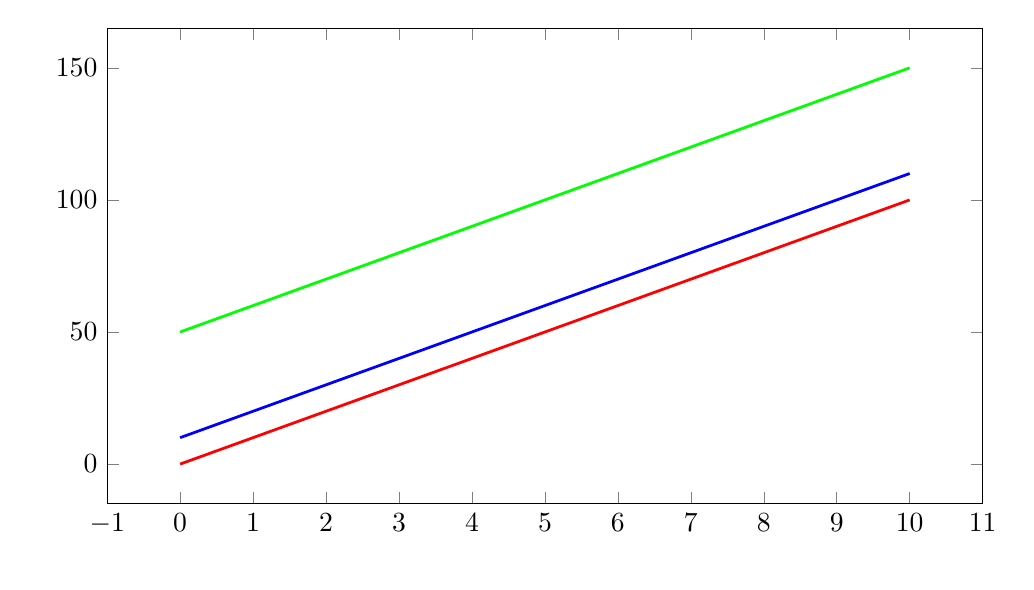
\begin{tikzpicture}[line width=1]
\begin{axis}[width=5in, height=3in,
             scatter/classes={a={mark=*,draw=black}},
             xlabel={\mbox{}},
             xlabel style={name=xlabel}, 
             ylabel={\mbox{}}, 
             legend style={
                at={(xlabel.south)},
                yshift=-1ex,
                anchor=north,
                legend cell align=left,
                },
        ]
]
\addplot[draw=red, line width=1] coordinates {(0.0,0.0)
(5.0,50.0)
(10.0,100.0)
(10.0,100.0)};\addplot[draw=blue, line width=1] coordinates {(0.0,10.0)
(5.0,60.0)
(10.0,110.0)
(10.0,110.0)};\addplot[draw=green, line width=1] coordinates {(0.0,50.0)
(5.0,100.0)
(10.0,150.0)
(10.0,150.0)};
\end{axis}\end{tikzpicture}\end{center}


(I'm not labeling the graphs
because you should be able to tell which is which ... right?)
For small values of $n$, i.e., $0 \leq n \leq 10$, the functions
are different and separated from each other.
But now if I increase the values for $n$, say, $0 \leq n \leq 100$, 
they look like this:
%-*-latex-*-

\begin{center}
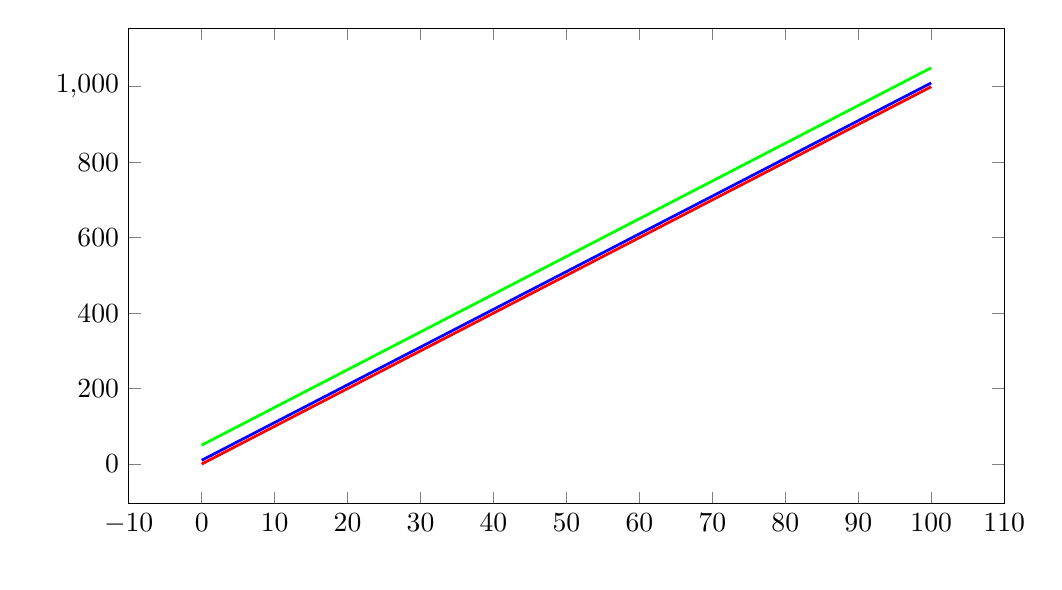
\begin{tikzpicture}[line width=1]
\begin{axis}[width=5in, height=3in,
             scatter/classes={a={mark=*,draw=black}},
             xlabel={\mbox{}},
             xlabel style={name=xlabel}, 
             ylabel={\mbox{}}, 
             legend style={
                at={(xlabel.south)},
                yshift=-1ex,
                anchor=north,
                legend cell align=left,
                },
        ]
]
\addplot[draw=red, line width=1] coordinates {(0.0,0.0)
(50.0,500.0)
(100.0,1000.0)
(100.0,1000.0)};\addplot[draw=blue, line width=1] coordinates {(0.0,10.0)
(50.0,510.0)
(100.0,1010.0)
(100.0,1010.0)};\addplot[draw=green, line width=1] coordinates {(0.0,50.0)
(50.0,550.0)
(100.0,1050.0)
(100.0,1050.0)};
\end{axis}\end{tikzpicture}\end{center}


And here's the plot for the domain of $0 \leq n \leq 1000$:
%-*-latex-*-

\begin{center}
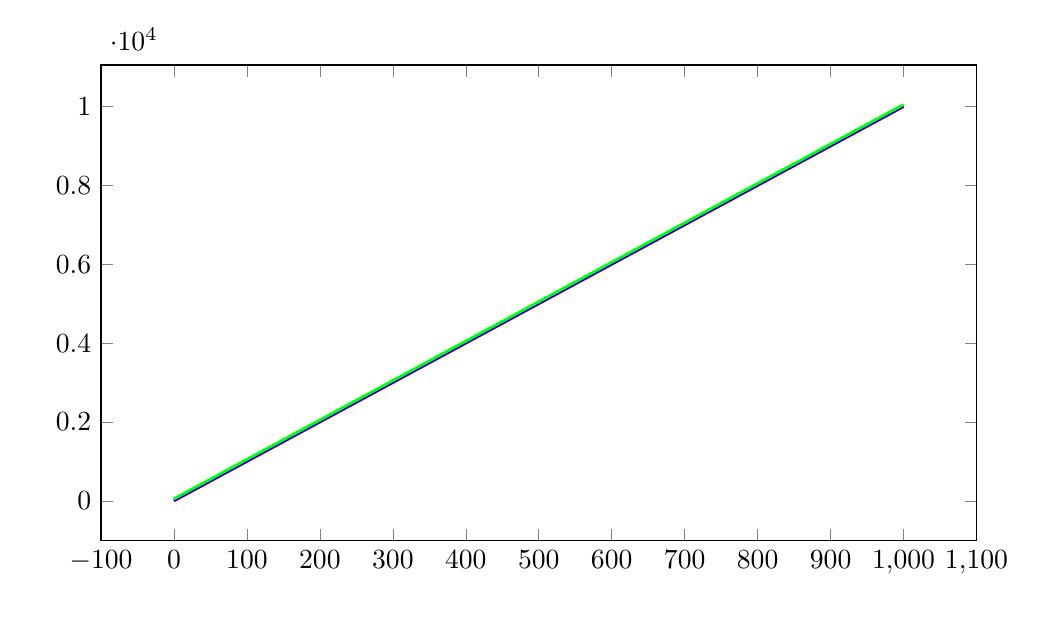
\begin{tikzpicture}[line width=1]
\begin{axis}[width=5in, height=3in,
             scatter/classes={a={mark=*,draw=black}},
             xlabel={\mbox{}},
             xlabel style={name=xlabel}, 
             ylabel={\mbox{}}, 
             legend style={
                at={(xlabel.south)},
                yshift=-1ex,
                anchor=north,
                legend cell align=left,
                },
        ]
]
\addplot[draw=red, line width=1] coordinates {(0.0,0.0)
(500.0,5000.0)
(1000.0,10000.0)
(1000.0,10000.0)};\addplot[draw=blue, line width=1] coordinates {(0.0,10.0)
(500.0,5010.0)
(1000.0,10010.0)
(1000.0,10010.0)};\addplot[draw=green, line width=1] coordinates {(0.0,50.0)
(500.0,5050.0)
(1000.0,10050.0)
(1000.0,10050.0)};
\end{axis}\end{tikzpicture}\end{center}

All three graphs more or less collapse into a single line, right?
You see that for large values of $n$,
the functions:
\[
y = 10n, \,\,\,\,\,
y = 10n + 10, \,\,\,\,\, 
y = 10n + 50
\]
really behave very much like each other: they all grow as fast as $10n$.

The second fudging step is when I throw away the $A$ 
in the function
\[
An
\]
and replace it by $1$ to get the function
\[
n
\]
because
the constant $A$ is hardware dependent
and has nothing to do with the inherent with the algorithm of the
pseudocode.
If you change your machine, your $t_5$ will either larger or smaller.
On the other hand, the $n$ in $An$ is inherent to the pseudocode -- it comes
from the loop.
You cannot remove the loop (or the $n$) just by changing your machine.
%Here's a plot of $y = n$, $y = 10n$, $y = 100n$
%for $0 \leq n \leq 10$:
%%-*-latex-*-

\begin{center}
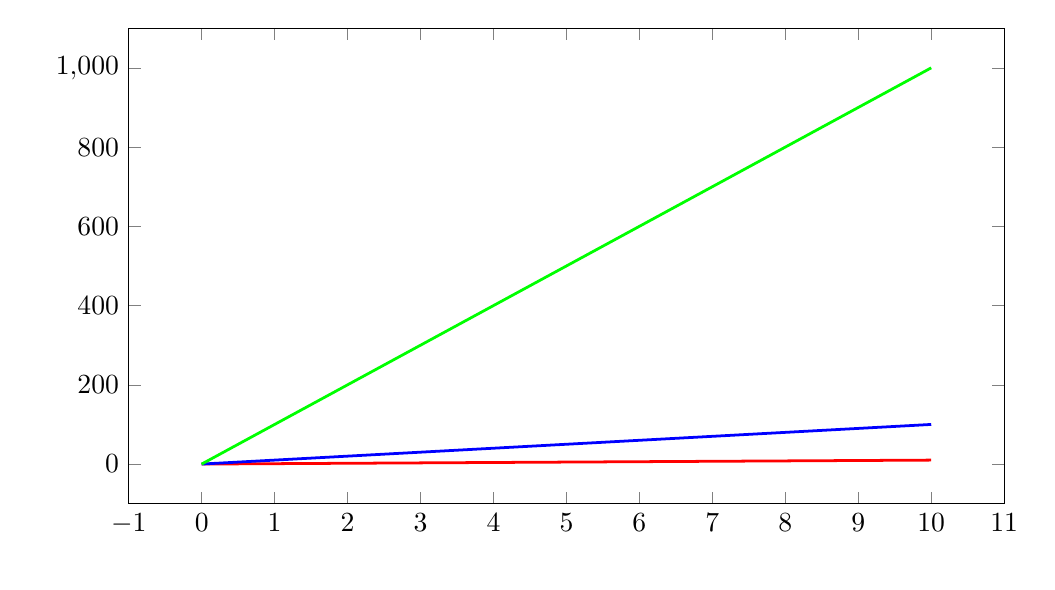
\begin{tikzpicture}[line width=1]
\begin{axis}[width=5in, height=3in,
             scatter/classes={a={mark=*,draw=black}},
             xlabel={\mbox{}},
             xlabel style={name=xlabel}, 
             ylabel={\mbox{}}, 
             legend style={
                at={(xlabel.south)},
                yshift=-1ex,
                anchor=north,
                legend cell align=left,
                },
        ]
]
\addplot[draw=red, line width=1] coordinates {(0.0,0.0)
(5.0,5.0)
(10.0,10.0)
(10.0,10.0)};\addplot[draw=blue, line width=1] coordinates {(0.0,0.0)
(5.0,50.0)
(10.0,100.0)
(10.0,100.0)};\addplot[draw=green, line width=1] coordinates {(0.0,0.0)
(5.0,500.0)
(10.0,1000.0)
(10.0,1000.0)};
\end{axis}\end{tikzpicture}\end{center}

%
%For $1000 \leq n \leq 10000$:
%%-*-latex-*-

\begin{center}
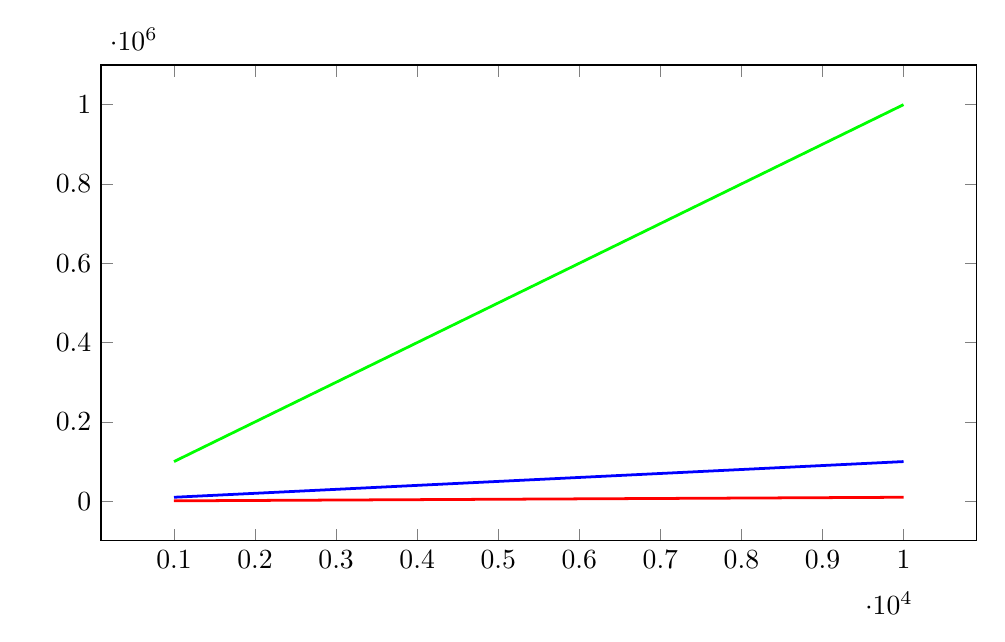
\begin{tikzpicture}[line width=1]
\begin{axis}[width=5in, height=3in,
             scatter/classes={a={mark=*,draw=black}},
             xlabel={\mbox{}},
             xlabel style={name=xlabel}, 
             ylabel={\mbox{}}, 
             legend style={
                at={(xlabel.south)},
                yshift=-1ex,
                anchor=north,
                legend cell align=left,
                },
        ]
]
\addplot[draw=red, line width=1] coordinates {(1000.0,1000.0)
(5500.0,5500.0)
(10000.0,10000.0)
(10000.0,10000.0)};\addplot[draw=blue, line width=1] coordinates {(1000.0,10000.0)
(5500.0,55000.0)
(10000.0,100000.0)
(10000.0,100000.0)};\addplot[draw=green, line width=1] coordinates {(1000.0,100000.0)
(5500.0,550000.0)
(10000.0,1000000.0)
(10000.0,1000000.0)};
\end{axis}\end{tikzpicture}\end{center}

%They are constant multiples of each other.
%And remember this important fact:
%I don't care about multiple differences since 
%in the case of functions measuring resource use (time in our case)
%it just mean that there's a difference in the hardware used.
Also,
you will see later that when we compare multiples of $n$ with
multiples of $n^2$ and multiples of $n^3$, you will see that the
when $n$ is huge,
multiples of $n$ clump together closely and away from the multiples of
$n^2$ and $n^3$.
You will also see that multiples of $n^2$ clump up together away from the 
multiples of $n^3$.
I'll show you some examples in the next section.

By the way, you can measure any resource taken up by an algorithm.
For instance you can also measure the \defone{space complexity} of an
algorithm, i.e., the amount of \textit{extra} memory needed to carry out 
an algorithm.

For the sum from 1 to $n$ algorithm, you are given $n$
and you need to store the result in $s$.
Any memory usage besides $n$ and $s$ (the memory
usage for input and output) is considered extra memory.
For our algorithm
\begin{Verbatim}[frame=single, fontsize=\footnotesize]
s = 0
for i = 1, 2, ..., n:
     s = s + i
\end{Verbatim}
The extra memory usage is due to variable $i$.
The variable \verb!s! is not considered extra -- you have to compute
\verb!s! since that's the goal of the algorithm.
Memory is frequently measured in bytes or bits.
(For serious theoretical CS, bits is used.)
Being an integer, $i$ might use up $4$ bytes.
I would then say the space complexity of our sum from 1 to $n$ algorithm is
\[
\textsc{Space}(n) = 4
\]
Since $4 = 4 \cdot n^0$, I will use the big-O notiation and write
\[
\textsc{Space}(n) = O(n^0) = O(1)
\]
In you prefer to use bits instead of bits, 4 bytes is 32 bits, which is then
\[
\textsc{Space}(n) = 32
\]
But $32 = 32 \cdot n^0$, so
\[
\textsc{Space}(n) = O(n^0) = O(1)
\]
which gives the same space complexity as when I use bytes to measure
memory usage.
It's also clear that you can also count the number of integer variables
(i.e., count 4-bytes) and arrive at the same space complexity.
In this case, I will say that the algorithm has
\defone{constant space complexity}.
Altogether for my sum from 1 to $n$ algorithm:
\begin{align*}
  T(n) &= O(n) \\
  \mathsc{Space}(n) &= O(1)
\end{align*}
  
\newpage
\begin{ex} 
  \label{ex:some-decision1}
  \tinysidebar{\debug{exercises/{empty0/question.tex}}}
  \solutionlink{sol:some-decision1}
  \qed
\end{ex} 
\begin{python0}
from solutions import *
add(label="ex:some-decision1",
    srcfilename='exercises/some-decision1/answer.tex') 
\end{python0}

\newpage
\begin{ex} 
  \label{ex:some-decision1}
  \tinysidebar{\debug{exercises/{empty0/question.tex}}}
  \solutionlink{sol:some-decision1}
  \qed
\end{ex} 
\begin{python0}
from solutions import *
add(label="ex:some-decision1",
    srcfilename='exercises/some-decision1/answer.tex') 
\end{python0}

\newpage
\begin{ex} 
  \label{ex:some-decision1}
  \tinysidebar{\debug{exercises/{empty0/question.tex}}}
  \solutionlink{sol:some-decision1}
  \qed
\end{ex} 
\begin{python0}
from solutions import *
add(label="ex:some-decision1",
    srcfilename='exercises/some-decision1/answer.tex') 
\end{python0}

\newpage
\begin{ex} 
  \label{ex:some-decision1}
  \tinysidebar{\debug{exercises/{empty0/question.tex}}}
  \solutionlink{sol:some-decision1}
  \qed
\end{ex} 
\begin{python0}
from solutions import *
add(label="ex:some-decision1",
    srcfilename='exercises/some-decision1/answer.tex') 
\end{python0}

\newpage
\begin{ex} 
  \label{ex:some-decision1}
  \tinysidebar{\debug{exercises/{empty0/question.tex}}}
  \solutionlink{sol:some-decision1}
  \qed
\end{ex} 
\begin{python0}
from solutions import *
add(label="ex:some-decision1",
    srcfilename='exercises/some-decision1/answer.tex') 
\end{python0}

\newpage
\begin{ex} 
  \label{ex:some-decision1}
  \tinysidebar{\debug{exercises/{empty0/question.tex}}}
  \solutionlink{sol:some-decision1}
  \qed
\end{ex} 
\begin{python0}
from solutions import *
add(label="ex:some-decision1",
    srcfilename='exercises/some-decision1/answer.tex') 
\end{python0}


\newpage%-*-latex-*-
\sectionthree{Best, average, and worst runtime}
\begin{python0}
from solutions import *; clear()
\end{python0}

Now let me consider an algorithm 
when the body of the for-loop 
contains an \verb!if!-statement.

The following computes the index in an (unsorted) 
array \verb!x! of size \verb!n!
where \verb!target! is 
first found, i.e., this is the linear search algorithm:

\begin{Verbatim}[frame=single, fontsize=\footnotesize]
index = -1
for i = 0, 1, 2, ..., n - 1:
    if x[i] is target:
        index = i
        break
\end{Verbatim}
Here's the above written in a way that makes timing calculation easier:
\begin{Verbatim}[frame=single, fontsize=\footnotesize]
                                 time   
         index = -1              t1 
         i = 0                   t2 
LOOP:    if i >= n:              t3  
             goto ENDLOOP        t4 
         if x[i] is not target:  t5
             goto ELSE           t6
         index = i               t7 
         goto ENDLOOP            t8
ELSE:    i = i + 1               t9 
         goto LOOP               t10 
ENDLOOP:
\end{Verbatim}

(For non-programmers:
when I say array \verb!x! is an array of size \verb!n! I mean that
you have \verb!x[0]!, \verb!x[1]!, \ldots, \verb!x[n-1]!
which is similar to the mathematical idea of 
a bunch of variables with scripts $x_0$, $x_1$, $\ldots$, $x_{n-1}$.
\verb!break! means to get out of the current loop.
The time to access the \verb!i!--th element \verb!x[i]! of \verb!x! is
constant.)

The amount of time needed of course depends on how fast we hit \verb!target!:
if \verb!target! happens to be at index 0, of course the algorithm ends
quickly. 
This is the best case scenario.
And if \verb!target! is at index $n-1$ or if it's not even in the array,
the algorithm would run longer since you would have to scan the whole array.
These are the worst case scenarios.

Note that in my first timing example that computes the sum from 1 to $n$,
I converted a for-loop into statements of a simplified
language that uses the goto and the
conditional branching statement.
For the above example, it's easy to see that if you have an algorithm
that has an if-else statement such as
\begin{Verbatim}[frame=single, fontsize=\footnotesize]
if x > 1:
    statement-1
    statement-2
else:
    statement-3    
    statement-4
\end{Verbatim}
you can rewrite that in the simplified language as
\begin{Verbatim}[frame=single, fontsize=\footnotesize]
         if x <= 1:
             goto ELSE
         statement-1
         statement-2
         goto ENDIF
ELSE:    statement-3
         statement-4
ENDIF:         
\end{Verbatim}
Note that the conditional branching leads to the else case, and therefore
the boolean condition is the opposite of the boolean condition of the
if-else statement.
Now let's go back to the timing calculations.

Here's the timing calculation for the best scenario:
\begin{Verbatim}[frame=single, fontsize=\footnotesize]
                                   time    number of times   
         index = -1                t1      1
         i = 0                     t2      1
LOOP:    if i >= n:                t3      1
             goto ENDLOOP          t4      0
         if x[i] is not target:    t5      1
             goto ELSE             t6      0
         index = i                 t7      1
         goto ENDLOOP              t8      1
ELSE:    i = i + 1                 t9      0
         goto LOOP                 t10     0
ENDLOOP:
\end{Verbatim}
The time taken is
\begin{align*}
\text{Time taken } 
&= A
\end{align*}
for some constant $A$.
In this case the constant function $f(n) = A$
is a constant multiple of the simpler function $g(n) = 1$.
Since we ignore multiples, I can say that for this 
\lq\lq optimistic'' case, the runtime is $O(1)$.
Mathemtically, I can write this:
\begin{align*}
\text{Time taken } 
&= A = O(1)
\end{align*}

For the worst case where the \verb!target! is the last element of the array,
i.e., at index \verb!n - 1!,
we have the following:
\begin{Verbatim}[frame=single, fontsize=\footnotesize]
                                   time     number of times   
         index = -1                t1       1
         i = 0                     t2       1
LOOP:    if i >= n:                t3       n
             goto ENDLOOP          t4       0
         if x[i] is not target:    t5       n 
             goto ELSE             t6       n - 1
         index = i                 t7       1
         goto ENDLOOP              t8       1
ELSE:    i = i + 1                 t9       n - 1
         goto LOOP                 t10      n - 1
ENDLOOP:
\end{Verbatim}
The time taken is
\begin{align*}
\text{Time taken } 
&= t_1 + t_2 + t_7 + t_8 + 
   (t_3 + t_5)n + 
   (t_6 + t_9 + t_{10})(n - 1) \\
&= (t_3 + t_5 + t_6 + t_9 + t_{10})n +
   (t_1 + t_2 - t_6 + t_7 
    + t_8 - t_9 - t_{10}) \\ 
&= An + B
\end{align*}
for constants $A$ and $B$.
In this case the runtime function is big-O of $n$, i.e., it is 
$O(n)$.
I write:
The time taken is
\[
\text{Time taken } 
= An + B = O(n)
\]

For the worst case where the \verb!target! is not found
we have the following:
\begin{Verbatim}[frame=single, fontsize=\footnotesize]
                                   time    number of times   
         index = -1                t1      1
         i = 0                     t2      1
LOOP:    if i >= n:                t3      n + 1
             goto ENDLOOP          t4      1
         if x[i] is not target:    t5      n 
             goto ELSE             t6      n
         index = i                 t7      0
         goto ENDLOOP              t8      0
ELSE:    i = i + 1                 t9      n
         goto LOOP                 t10     n
ENDLOOP:
\end{Verbatim}
The time taken is
\begin{align*}
\text{Time taken } 
  &= t_1 + t_2 + 
    t_4 + 
    n(t_3 + t_5 + t_6 + t_9 + t_{10}) +
    (n + 1) t_3 \\
  &= n(t_3 + t_5 + 
    t_6  + 
    t_9 +
    t_{10}
    )
    +
    t_1 + 
    t_2 + 
    t_3 + 
    t_4 \\
&= An + B \\
&= O(n)
\end{align*}
for constants $A$ and $B$.
In the second worst case scenario,
the runtime function is also big-O of $n$, 
i.e., it is $O(n)$.

In summary the best runtime and the two worst runtimes are
\begin{align*}
A_1 &= O(1) \\
A_2n + B_2 &= O(n) \\
A_3n + B_3 &= O(n) 
\end{align*}

Usually performance of algorithms are described in terms of
best, worst, and average times.
If you want to lump up all the runtimes (i.e., you don't really want to
be that specific), we want to say that runtime is $O(n)$, 
referring to the absolute worst scenario.

In other words you should think of the big-O notation $O(n)$
as some kind of \textit{upper} bound approximation, i.e.,
all the above times are bounded above by a large enough multiple of $n$:
\begin{align*}
A_1        &\leq C \cdot n \\
A_2n + B_2 &\leq C \cdot n \\
A_3n + B_3 &\leq C \cdot n
\end{align*}
where $C$ is some humongous fixed number and the above inequalities
are true for large values of $n$.

While talking about a specific algorithm, to distinguish between
the best, worst, and average runtime, I will write
$T_{b}(n)$,
$T_{w}(n)$,
and
$T_{a}(n)$.
(Technically speaking there are two different worst case scenarios
for the linear search above.
But they both yield the same big-O anyway.)

If I don't say which of the three cases, I always mean the 
worst case $T_w(n)$.

I have shown you above that for the linear search
\begin{align*}
T_b(n) &= O(1) \\
T_w(n) &= O(n)
\end{align*}

The average case is a little more complicated.
In the above linear search algorithm, we looked at
three cases (one best and two worst).
But in general, the \verb!target! can be anywhere and you would have to 
account for all of them, measure their times, 
say we call them $T_0(n)$, ..., $T_n(n)$
where the algorithm has $n + 1$ cases
($T_0(n)$ corresponding to the time where the \verb!target! is at index 0, ...
and $T_n(n)$ corresponding to the time where the \verb!target! is not
in the array at all)
and then take the average:
\[
\frac{T_0(n) + \cdots + T_n(n)}{n + 1}
\]
But that assume something: 
That the cases corresponding to times $T_0(n)$, ..., $T_n(n)$ are
equally likely to occur.

Depending on specific scenario, 
there are cases that might occur more frequently.
For instance if in the above, the case where the index 0 occurs twice
as frequently as the rest, then the average would be
\[
\frac{2T_0(n) + \cdots + T_n(n)}{n + 2}
\]
To analyze the average runtime for
complicated cases require a little more probability theory.
For now we will only handle very simplisitic average cases.

In general, to compute \textit{an} (not \textit{the}) 
average runtime, you have to 
\begin{enumerate}[nosep]
\item[(1)] state what cases you're average over and 
\item[(2)] what is the likelihood of each case.
\end{enumerate}
When the cases are not stated, they are usually obvious.
Also, if the likelihood of each case is not stated, then it is assumed
that all cases are equally likely.

For many algorithms and many average scenarios, 
the average runtimes tend to be
the same as the worst runtime when you fudge the functions using big-O. 

Now that I've explained how to compute the average runtime, let's
compute the average runtime of the linear search assuming that we
are only averaging over the cases where
\verb!target! is at index $0, 1, 2, ...,  n - 1$.
Note that I'm not considering the case 
where \verb!target! is not in the array.
If you like you can think of this as the 
\lq\lq average runtime for a successful search''.
(In a later section, I'll include the case where the \verb!target!
is not in the array -- this is just slightly more complicated.)

Let me assume that \verb!target! is at index value $k$
where $0 \leq k \leq n - 1$.
Here's the number of times each statement will execute in this case:
\begin{Verbatim}[frame=single, fontsize=\footnotesize]
                                   time    number of times   
         index = -1                t1      1
         i = 0                     t2      1
LOOP:    if i >= n:                t3      k + 1
             goto ENDLOOP          t4      0
         if x[i] is not target:    t5      k + 1 
             goto ELSE             t6      k 
         index = i                 t7      1
         goto ENDLOOP              t8      1
ELSE:    i = i + 1                 t9      k
         goto LOOP                 t10     k
ENDLOOP:
\end{Verbatim}
Therefore time taken for this case is
\begin{align*}
T_k(n)
  &= (t_1 + t_2 + t_7 + t_8)
    + (t_3 + t_5)(k + 1)
    + (t_6 + t_9 + t_{10})k \\
  &= (t_3 + t_5 + t_6 + t_9 + t_{10}) k
    + (t_1 + t_2 + t_3 + t_5 + t_7 + t_8)
\end{align*}
for $k = 0, 1, 2, ..., n - 1$.
Let $T_n$ be the time corresponding to the case where
\verb!target! is \textit{not} in the array.
Earlier, I have already compute the runtime for the case where 
\verb!target! is not in the array:
\[
  T_n(n) =
  (t_3 + t_5 + 
    t_6  + 
    t_9 +
    t_{10}
    )n
    +
    t_1 + 
    t_2 + 
    t_3 + 
    t_4
\]
To simplify the constants 
(because later, we'll be computing by big-O anyway),
let
\begin{align*}
A &= t_3 + t_5 + t_6 + t_9 + t_{10} \\
B &= t_1 + t_2 + t_3 + t_5 + t_7 + t_8 \\
C &= t_3 + t_5 + 
    t_6  + 
    t_9 +
    t_{10} \\
D &= t_1 + 
    t_2 + 
    t_3 + 
    t_4
\end{align*}
Here's a summary:
\begin{align*}
T_k(n) &= Ak + B, \,\,\,\,\,(k = 0, 1, 2,..., n - 1) \\
T_n(n) &= Cn + D
\end{align*}

OK, now I'm going to compute the average runtime
assuming 
\begin{itemize}
\item the \verb!target! is in the array with equal likelihood
at all index positions.
\end{itemize}

Remember: This average runtime scenario
does \textit{not} include the case where the \verb!target!
is not in array \verb!x!.
So I need to average over $T_0(n), \ldots, T_{n-1}(n-1)$ ... 
do \textit{not} include $T_n(n)$.

This average runtime is
\begin{align*}
T_a(n) 
&= \frac{1}{n} 
   \left(
     T_0(n) + T_1(n) + \cdots + T_{n - 1}(n) 
   \right)
\\
&= \frac{1}{n}
   \left(
     (A\cdot 0 + B) + 
     (A\cdot 1 + B) + 
     \cdots
     (A\cdot (n - 1) + B)
   \right)
\\
&= \frac{1}{n}
   \left(
     A\cdot (0 + 1 + \cdots + (n - 1))
     + Bn 
   \right)
\\
&= \frac{1}{n}
   \left(
     A \cdot \frac{n(n-1)}{2} + Bn
   \right)
\\
&= \frac{1}{n}
   \left( 
     \frac{A}{2} n^2
     + \left( B - \frac{1}{2}A \right) n
   \right)
\\
&= \frac{A}{2} n
   + \left( B - \frac{1}{2}A \right)
\\
&= O(n)
\end{align*}


That's it!

\newpage
\begin{ex} 
  \label{ex:some-decision1}
  \tinysidebar{\debug{exercises/{empty0/question.tex}}}
  \solutionlink{sol:some-decision1}
  \qed
\end{ex} 
\begin{python0}
from solutions import *
add(label="ex:some-decision1",
    srcfilename='exercises/some-decision1/answer.tex') 
\end{python0}

\newpage
\begin{ex} 
  \label{ex:some-decision1}
  \tinysidebar{\debug{exercises/{empty0/question.tex}}}
  \solutionlink{sol:some-decision1}
  \qed
\end{ex} 
\begin{python0}
from solutions import *
add(label="ex:some-decision1",
    srcfilename='exercises/some-decision1/answer.tex') 
\end{python0}

\newpage
\begin{ex} 
  \label{ex:some-decision1}
  \tinysidebar{\debug{exercises/{empty0/question.tex}}}
  \solutionlink{sol:some-decision1}
  \qed
\end{ex} 
\begin{python0}
from solutions import *
add(label="ex:some-decision1",
    srcfilename='exercises/some-decision1/answer.tex') 
\end{python0}

\newpage
\begin{ex} 
  \label{ex:some-decision1}
  \tinysidebar{\debug{exercises/{empty0/question.tex}}}
  \solutionlink{sol:some-decision1}
  \qed
\end{ex} 
\begin{python0}
from solutions import *
add(label="ex:some-decision1",
    srcfilename='exercises/some-decision1/answer.tex') 
\end{python0}

\newpage
\begin{ex} 
  \label{ex:some-decision1}
  \tinysidebar{\debug{exercises/{empty0/question.tex}}}
  \solutionlink{sol:some-decision1}
  \qed
\end{ex} 
\begin{python0}
from solutions import *
add(label="ex:some-decision1",
    srcfilename='exercises/some-decision1/answer.tex') 
\end{python0}

 
\newpage%-*-latex-*-
\sectionthree{Separating polynomial functions}
\begin{python0}
from solutions import *; clear()
\end{python0}

I'll be giving you the formal definition of big-O soon.
But before that, I'm going to motivate the (formal) definition of big-O
by talking about the way the graphs of polynomial climb.
The rate at which they climb essentially tells you the story of big-O among 
polynomials.
This will give you the intuitive idea behind big-O before I hit you
with the formal definition.

In this section, I will show you that when you plot polynomial functions,
they bunch up into groups.
These groups are very well-defined and simple:
they are determined by the \textit{degree} of polynomials.

Look at this mess of 15 polynomial functions 
(I won't give you the polynomials just yet):
%-*-latex-*-

\begin{center}
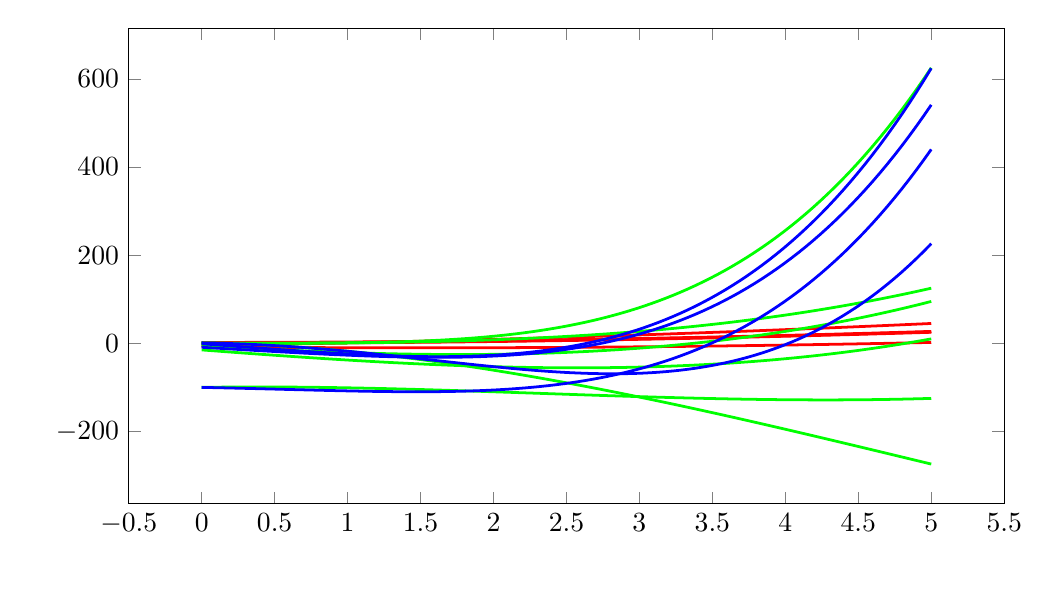
\begin{tikzpicture}[line width=1]
\begin{axis}[width=5in, height=3in,
             scatter/classes={a={mark=*,draw=black}},
             xlabel={\mbox{}},
             xlabel style={name=xlabel}, 
             ylabel={\mbox{}}, 
             legend style={
                at={(xlabel.south)},
                yshift=-1ex,
                anchor=north,
                legend cell align=left,
                },
        ]
]
\addplot[draw=red, line width=1] coordinates {(0.0,0.0)
(0.0505,0.0026)
(0.101,0.0102)
(0.1515,0.023)
(0.202,0.0408)
(0.2525,0.0638)
(0.303,0.0918)
(0.3535,0.125)
(0.404,0.1632)
(0.4545,0.2066)
(0.5051,0.2551)
(0.5556,0.3086)
(0.6061,0.3673)
(0.6566,0.4311)
(0.7071,0.4999)
(0.7576,0.5739)
(0.8081,0.653)
(0.8586,0.7372)
(0.9091,0.8264)
(0.9596,0.9208)
(1.0101,1.0203)
(1.0606,1.1249)
(1.1111,1.2346)
(1.1616,1.3494)
(1.2121,1.4692)
(1.2626,1.5942)
(1.3131,1.7243)
(1.3636,1.8595)
(1.4141,1.9998)
(1.4646,2.1452)
(1.5152,2.2957)
(1.5657,2.4513)
(1.6162,2.612)
(1.6667,2.7778)
(1.7172,2.9487)
(1.7677,3.1247)
(1.8182,3.3058)
(1.8687,3.492)
(1.9192,3.6833)
(1.9697,3.8797)
(2.0202,4.0812)
(2.0707,4.2878)
(2.1212,4.4995)
(2.1717,4.7164)
(2.2222,4.9383)
(2.2727,5.1653)
(2.3232,5.3974)
(2.3737,5.6346)
(2.4242,5.877)
(2.4747,6.1244)
(2.5253,6.3769)
(2.5758,6.6345)
(2.6263,6.8973)
(2.6768,7.1651)
(2.7273,7.438)
(2.7778,7.716)
(2.8283,7.9992)
(2.8788,8.2874)
(2.9293,8.5808)
(2.9798,8.8792)
(3.0303,9.1827)
(3.0808,9.4914)
(3.1313,9.8051)
(3.1818,10.124)
(3.2323,10.4479)
(3.2828,10.777)
(3.3333,11.1111)
(3.3838,11.4504)
(3.4343,11.7947)
(3.4848,12.1442)
(3.5354,12.4987)
(3.5859,12.8584)
(3.6364,13.2231)
(3.6869,13.593)
(3.7374,13.968)
(3.7879,14.348)
(3.8384,14.7332)
(3.8889,15.1235)
(3.9394,15.5188)
(3.9899,15.9193)
(4.0404,16.3249)
(4.0909,16.7355)
(4.1414,17.1513)
(4.1919,17.5722)
(4.2424,17.9982)
(4.2929,18.4292)
(4.3434,18.8654)
(4.3939,19.3067)
(4.4444,19.7531)
(4.4949,20.2046)
(4.5455,20.6612)
(4.596,21.1228)
(4.6465,21.5896)
(4.697,22.0615)
(4.7475,22.5385)
(4.798,23.0206)
(4.8485,23.5078)
(4.899,24.0001)
(4.9495,24.4975)
(5.0,25.0)
(5.0,25.0)};\addplot[draw=red, line width=1] coordinates {(0.0,2.0)
(0.0505,2.0026)
(0.101,2.0102)
(0.1515,2.023)
(0.202,2.0408)
(0.2525,2.0638)
(0.303,2.0918)
(0.3535,2.125)
(0.404,2.1632)
(0.4545,2.2066)
(0.5051,2.2551)
(0.5556,2.3086)
(0.6061,2.3673)
(0.6566,2.4311)
(0.7071,2.4999)
(0.7576,2.5739)
(0.8081,2.653)
(0.8586,2.7372)
(0.9091,2.8264)
(0.9596,2.9208)
(1.0101,3.0203)
(1.0606,3.1249)
(1.1111,3.2346)
(1.1616,3.3494)
(1.2121,3.4692)
(1.2626,3.5942)
(1.3131,3.7243)
(1.3636,3.8595)
(1.4141,3.9998)
(1.4646,4.1452)
(1.5152,4.2957)
(1.5657,4.4513)
(1.6162,4.612)
(1.6667,4.7778)
(1.7172,4.9487)
(1.7677,5.1247)
(1.8182,5.3058)
(1.8687,5.492)
(1.9192,5.6833)
(1.9697,5.8797)
(2.0202,6.0812)
(2.0707,6.2878)
(2.1212,6.4995)
(2.1717,6.7164)
(2.2222,6.9383)
(2.2727,7.1653)
(2.3232,7.3974)
(2.3737,7.6346)
(2.4242,7.877)
(2.4747,8.1244)
(2.5253,8.3769)
(2.5758,8.6345)
(2.6263,8.8973)
(2.6768,9.1651)
(2.7273,9.438)
(2.7778,9.716)
(2.8283,9.9992)
(2.8788,10.2874)
(2.9293,10.5808)
(2.9798,10.8792)
(3.0303,11.1827)
(3.0808,11.4914)
(3.1313,11.8051)
(3.1818,12.124)
(3.2323,12.4479)
(3.2828,12.777)
(3.3333,13.1111)
(3.3838,13.4504)
(3.4343,13.7947)
(3.4848,14.1442)
(3.5354,14.4987)
(3.5859,14.8584)
(3.6364,15.2231)
(3.6869,15.593)
(3.7374,15.968)
(3.7879,16.348)
(3.8384,16.7332)
(3.8889,17.1235)
(3.9394,17.5188)
(3.9899,17.9193)
(4.0404,18.3249)
(4.0909,18.7355)
(4.1414,19.1513)
(4.1919,19.5722)
(4.2424,19.9982)
(4.2929,20.4292)
(4.3434,20.8654)
(4.3939,21.3067)
(4.4444,21.7531)
(4.4949,22.2046)
(4.5455,22.6612)
(4.596,23.1228)
(4.6465,23.5896)
(4.697,24.0615)
(4.7475,24.5385)
(4.798,25.0206)
(4.8485,25.5078)
(4.899,26.0001)
(4.9495,26.4975)
(5.0,27.0)
(5.0,27.0)};\addplot[draw=red, line width=1] coordinates {(0.0,1.0)
(0.0505,1.0026)
(0.101,1.0102)
(0.1515,1.023)
(0.202,1.0408)
(0.2525,1.0638)
(0.303,1.0918)
(0.3535,1.125)
(0.404,1.1632)
(0.4545,1.2066)
(0.5051,1.2551)
(0.5556,1.3086)
(0.6061,1.3673)
(0.6566,1.4311)
(0.7071,1.4999)
(0.7576,1.5739)
(0.8081,1.653)
(0.8586,1.7372)
(0.9091,1.8264)
(0.9596,1.9208)
(1.0101,2.0203)
(1.0606,2.1249)
(1.1111,2.2346)
(1.1616,2.3494)
(1.2121,2.4692)
(1.2626,2.5942)
(1.3131,2.7243)
(1.3636,2.8595)
(1.4141,2.9998)
(1.4646,3.1452)
(1.5152,3.2957)
(1.5657,3.4513)
(1.6162,3.612)
(1.6667,3.7778)
(1.7172,3.9487)
(1.7677,4.1247)
(1.8182,4.3058)
(1.8687,4.492)
(1.9192,4.6833)
(1.9697,4.8797)
(2.0202,5.0812)
(2.0707,5.2878)
(2.1212,5.4995)
(2.1717,5.7164)
(2.2222,5.9383)
(2.2727,6.1653)
(2.3232,6.3974)
(2.3737,6.6346)
(2.4242,6.877)
(2.4747,7.1244)
(2.5253,7.3769)
(2.5758,7.6345)
(2.6263,7.8973)
(2.6768,8.1651)
(2.7273,8.438)
(2.7778,8.716)
(2.8283,8.9992)
(2.8788,9.2874)
(2.9293,9.5808)
(2.9798,9.8792)
(3.0303,10.1827)
(3.0808,10.4914)
(3.1313,10.8051)
(3.1818,11.124)
(3.2323,11.4479)
(3.2828,11.777)
(3.3333,12.1111)
(3.3838,12.4504)
(3.4343,12.7947)
(3.4848,13.1442)
(3.5354,13.4987)
(3.5859,13.8584)
(3.6364,14.2231)
(3.6869,14.593)
(3.7374,14.968)
(3.7879,15.348)
(3.8384,15.7332)
(3.8889,16.1235)
(3.9394,16.5188)
(3.9899,16.9193)
(4.0404,17.3249)
(4.0909,17.7355)
(4.1414,18.1513)
(4.1919,18.5722)
(4.2424,18.9982)
(4.2929,19.4292)
(4.3434,19.8654)
(4.3939,20.3067)
(4.4444,20.7531)
(4.4949,21.2046)
(4.5455,21.6612)
(4.596,22.1228)
(4.6465,22.5896)
(4.697,23.0615)
(4.7475,23.5385)
(4.798,24.0206)
(4.8485,24.5078)
(4.899,25.0001)
(4.9495,25.4975)
(5.0,26.0)
(5.0,26.0)};\addplot[draw=red, line width=1] coordinates {(0.0,-5.0)
(0.0505,-4.7449)
(0.101,-4.4847)
(0.1515,-4.2195)
(0.202,-3.9491)
(0.2525,-3.6736)
(0.303,-3.393)
(0.3535,-3.1073)
(0.404,-2.8165)
(0.4545,-2.5207)
(0.5051,-2.2197)
(0.5556,-1.9136)
(0.6061,-1.6024)
(0.6566,-1.2861)
(0.7071,-0.9647)
(0.7576,-0.6382)
(0.8081,-0.3066)
(0.8586,0.0301)
(0.9091,0.3719)
(0.9596,0.7188)
(1.0101,1.0708)
(1.0606,1.4279)
(1.1111,1.7901)
(1.1616,2.1574)
(1.2121,2.5298)
(1.2626,2.9074)
(1.3131,3.29)
(1.3636,3.6777)
(1.4141,4.0705)
(1.4646,4.4684)
(1.5152,4.8714)
(1.5657,5.2796)
(1.6162,5.6928)
(1.6667,6.1111)
(1.7172,6.5345)
(1.7677,6.9631)
(1.8182,7.3967)
(1.8687,7.8354)
(1.9192,8.2793)
(1.9697,8.7282)
(2.0202,9.1822)
(2.0707,9.6414)
(2.1212,10.1056)
(2.1717,10.5749)
(2.2222,11.0494)
(2.2727,11.5289)
(2.3232,12.0136)
(2.3737,12.5033)
(2.4242,12.9982)
(2.4747,13.4981)
(2.5253,14.0032)
(2.5758,14.5133)
(2.6263,15.0286)
(2.6768,15.5489)
(2.7273,16.0744)
(2.7778,16.6049)
(2.8283,17.1406)
(2.8788,17.6814)
(2.9293,18.2272)
(2.9798,18.7782)
(3.0303,19.3343)
(3.0808,19.8954)
(3.1313,20.4617)
(3.1818,21.0331)
(3.2323,21.6095)
(3.2828,22.1911)
(3.3333,22.7778)
(3.3838,23.3696)
(3.4343,23.9664)
(3.4848,24.5684)
(3.5354,25.1755)
(3.5859,25.7877)
(3.6364,26.405)
(3.6869,27.0273)
(3.7374,27.6548)
(3.7879,28.2874)
(3.8384,28.9251)
(3.8889,29.5679)
(3.9394,30.2158)
(3.9899,30.8688)
(4.0404,31.5269)
(4.0909,32.1901)
(4.1414,32.8584)
(4.1919,33.5318)
(4.2424,34.2103)
(4.2929,34.8939)
(4.3434,35.5826)
(4.3939,36.2764)
(4.4444,36.9753)
(4.4949,37.6793)
(4.5455,38.3884)
(4.596,39.1026)
(4.6465,39.822)
(4.697,40.5464)
(4.7475,41.2759)
(4.798,42.0105)
(4.8485,42.7502)
(4.899,43.4951)
(4.9495,44.245)
(5.0,45.0)
(5.0,45.0)};\addplot[draw=red, line width=1] coordinates {(0.0,-8.0)
(0.0505,-8.149)
(0.101,-8.2928)
(0.1515,-8.4316)
(0.202,-8.5652)
(0.2525,-8.6938)
(0.303,-8.8173)
(0.3535,-8.9356)
(0.404,-9.0489)
(0.4545,-9.157)
(0.5051,-9.2601)
(0.5556,-9.358)
(0.6061,-9.4509)
(0.6566,-9.5386)
(0.7071,-9.6213)
(0.7576,-9.6988)
(0.8081,-9.7712)
(0.8586,-9.8386)
(0.9091,-9.9008)
(0.9596,-9.958)
(1.0101,-10.01)
(1.0606,-10.0569)
(1.1111,-10.0988)
(1.1616,-10.1355)
(1.2121,-10.1671)
(1.2626,-10.1937)
(1.3131,-10.2151)
(1.3636,-10.2314)
(1.4141,-10.2426)
(1.4646,-10.2488)
(1.5152,-10.2498)
(1.5657,-10.2457)
(1.6162,-10.2365)
(1.6667,-10.2222)
(1.7172,-10.2028)
(1.7677,-10.1783)
(1.8182,-10.1488)
(1.8687,-10.1141)
(1.9192,-10.0743)
(1.9697,-10.0294)
(2.0202,-9.9794)
(2.0707,-9.9243)
(2.1212,-9.8641)
(2.1717,-9.7988)
(2.2222,-9.7284)
(2.2727,-9.6529)
(2.3232,-9.5723)
(2.3737,-9.4866)
(2.4242,-9.3958)
(2.4747,-9.2999)
(2.5253,-9.1989)
(2.5758,-9.0927)
(2.6263,-8.9815)
(2.6768,-8.8652)
(2.7273,-8.7438)
(2.7778,-8.6173)
(2.8283,-8.4857)
(2.8788,-8.3489)
(2.9293,-8.2071)
(2.9798,-8.0602)
(3.0303,-7.9082)
(3.0808,-7.751)
(3.1313,-7.5888)
(3.1818,-7.4215)
(3.2323,-7.2491)
(3.2828,-7.0715)
(3.3333,-6.8889)
(3.3838,-6.7012)
(3.4343,-6.5083)
(3.4848,-6.3104)
(3.5354,-6.1073)
(3.5859,-5.8992)
(3.6364,-5.686)
(3.6869,-5.4676)
(3.7374,-5.2442)
(3.7879,-5.0156)
(3.8384,-4.782)
(3.8889,-4.5432)
(3.9394,-4.2994)
(3.9899,-4.0504)
(4.0404,-3.7963)
(4.0909,-3.5372)
(4.1414,-3.2729)
(4.1919,-3.0036)
(4.2424,-2.7291)
(4.2929,-2.4495)
(4.3434,-2.1649)
(4.3939,-1.8751)
(4.4444,-1.5802)
(4.4949,-1.2803)
(4.5455,-0.9752)
(4.596,-0.665)
(4.6465,-0.3498)
(4.697,-0.0294)
(4.7475,0.2961)
(4.798,0.6267)
(4.8485,0.9624)
(4.899,1.3031)
(4.9495,1.649)
(5.0,2.0)
(5.0,2.0)};\addplot[draw=green, line width=1] coordinates {(0.0,0.0)
(0.0505,0.0001)
(0.101,0.001)
(0.1515,0.0035)
(0.202,0.0082)
(0.2525,0.0161)
(0.303,0.0278)
(0.3535,0.0442)
(0.404,0.066)
(0.4545,0.0939)
(0.5051,0.1288)
(0.5556,0.1715)
(0.6061,0.2226)
(0.6566,0.283)
(0.7071,0.3535)
(0.7576,0.4348)
(0.8081,0.5277)
(0.8586,0.6329)
(0.9091,0.7513)
(0.9596,0.8836)
(1.0101,1.0306)
(1.0606,1.1931)
(1.1111,1.3717)
(1.1616,1.5674)
(1.2121,1.7809)
(1.2626,2.0129)
(1.3131,2.2643)
(1.3636,2.5357)
(1.4141,2.828)
(1.4646,3.1419)
(1.5152,3.4783)
(1.5657,3.8379)
(1.6162,4.2214)
(1.6667,4.6296)
(1.7172,5.0634)
(1.7677,5.5234)
(1.8182,6.0105)
(1.8687,6.5254)
(1.9192,7.069)
(1.9697,7.6418)
(2.0202,8.2449)
(2.0707,8.8788)
(2.1212,9.5445)
(2.1717,10.2426)
(2.2222,10.9739)
(2.2727,11.7393)
(2.3232,12.5394)
(2.3737,13.3751)
(2.4242,14.2472)
(2.4747,15.1563)
(2.5253,16.1033)
(2.5758,17.0889)
(2.6263,18.114)
(2.6768,19.1793)
(2.7273,20.2855)
(2.7778,21.4335)
(2.8283,22.624)
(2.8788,23.8577)
(2.9293,25.1356)
(2.9798,26.4582)
(3.0303,27.8265)
(3.0808,29.2411)
(3.1313,30.7029)
(3.1818,32.2126)
(3.2323,33.771)
(3.2828,35.3789)
(3.3333,37.037)
(3.3838,38.7462)
(3.4343,40.5071)
(3.4848,42.3206)
(3.5354,44.1874)
(3.5859,46.1083)
(3.6364,48.0841)
(3.6869,50.1156)
(3.7374,52.2035)
(3.7879,54.3486)
(3.8384,56.5516)
(3.8889,58.8134)
(3.9394,61.1348)
(3.9899,63.5164)
(4.0404,65.959)
(4.0909,68.4636)
(4.1414,71.0307)
(4.1919,73.6612)
(4.2424,76.3558)
(4.2929,79.1154)
(4.3434,81.9407)
(4.3939,84.8325)
(4.4444,87.7915)
(4.4949,90.8185)
(4.5455,93.9144)
(4.596,97.0797)
(4.6465,100.3155)
(4.697,103.6223)
(4.7475,107.001)
(4.798,110.4524)
(4.8485,113.9772)
(4.899,117.5763)
(4.9495,121.2503)
(5.0,125.0)
(5.0,125.0)};\addplot[draw=green, line width=1] coordinates {(0.0,-5.0)
(0.0505,-6.0023)
(0.101,-6.9886)
(0.1515,-7.958)
(0.202,-8.9097)
(0.2525,-9.8431)
(0.303,-10.7573)
(0.3535,-11.6516)
(0.404,-12.5251)
(0.4545,-13.3772)
(0.5051,-14.207)
(0.5556,-15.0137)
(0.6061,-15.7967)
(0.6566,-16.555)
(0.7071,-17.2881)
(0.7576,-17.995)
(0.8081,-18.675)
(0.8586,-19.3273)
(0.9091,-19.9512)
(0.9596,-20.5458)
(1.0101,-21.1105)
(1.0606,-21.6444)
(1.1111,-22.1468)
(1.1616,-22.6168)
(1.2121,-23.0538)
(1.2626,-23.4569)
(1.3131,-23.8254)
(1.3636,-24.1585)
(1.4141,-24.4554)
(1.4646,-24.7154)
(1.5152,-24.9377)
(1.5657,-25.1214)
(1.6162,-25.2659)
(1.6667,-25.3704)
(1.7172,-25.434)
(1.7677,-25.4561)
(1.8182,-25.4358)
(1.8687,-25.3723)
(1.9192,-25.265)
(1.9697,-25.113)
(2.0202,-24.9155)
(2.0707,-24.6718)
(2.1212,-24.3811)
(2.1717,-24.0427)
(2.2222,-23.6557)
(2.2727,-23.2194)
(2.3232,-22.733)
(2.3737,-22.1957)
(2.4242,-21.6068)
(2.4747,-20.9655)
(2.5253,-20.2711)
(2.5758,-19.5226)
(2.6263,-18.7195)
(2.6768,-17.8608)
(2.7273,-16.9459)
(2.7778,-15.9739)
(2.8283,-14.9442)
(2.8788,-13.8558)
(2.9293,-12.708)
(2.9798,-11.5002)
(3.0303,-10.2314)
(3.0808,-8.9009)
(3.1313,-7.508)
(3.1818,-6.0518)
(3.2323,-4.5317)
(3.2828,-2.9468)
(3.3333,-1.2963)
(3.3838,0.4205)
(3.4343,2.2044)
(3.4848,4.0561)
(3.5354,5.9765)
(3.5859,7.9663)
(3.6364,10.0263)
(3.6869,12.1572)
(3.7374,14.3599)
(3.7879,16.6351)
(3.8384,18.9835)
(3.8889,21.406)
(3.9394,23.9034)
(3.9899,26.4763)
(4.0404,29.1256)
(4.0909,31.852)
(4.1414,34.6563)
(4.1919,37.5394)
(4.2424,40.5019)
(4.2929,43.5446)
(4.3434,46.6683)
(4.3939,49.8738)
(4.4444,53.1619)
(4.4949,56.5332)
(4.5455,59.9887)
(4.596,63.5291)
(4.6465,67.1551)
(4.697,70.8675)
(4.7475,74.6671)
(4.798,78.5547)
(4.8485,82.531)
(4.899,86.5968)
(4.9495,90.7529)
(5.0,95.0)
(5.0,95.0)};\addplot[draw=green, line width=1] coordinates {(0.0,-15.0)
(0.0505,-16.2599)
(0.101,-17.514)
(0.1515,-18.7614)
(0.202,-20.0014)
(0.2525,-21.2333)
(0.303,-22.4561)
(0.3535,-23.6692)
(0.404,-24.8718)
(0.4545,-26.0631)
(0.5051,-27.2424)
(0.5556,-28.4088)
(0.6061,-29.5616)
(0.6566,-30.7)
(0.7071,-31.8233)
(0.7576,-32.9307)
(0.8081,-34.0214)
(0.8586,-35.0946)
(0.9091,-36.1495)
(0.9596,-37.1855)
(1.0101,-38.2016)
(1.0606,-39.1972)
(1.1111,-40.1715)
(1.1616,-41.1236)
(1.2121,-42.0529)
(1.2626,-42.9585)
(1.3131,-43.8397)
(1.3636,-44.6957)
(1.4141,-45.5257)
(1.4646,-46.329)
(1.5152,-47.1048)
(1.5657,-47.8523)
(1.6162,-48.5707)
(1.6667,-49.2593)
(1.7172,-49.9172)
(1.7677,-50.5438)
(1.8182,-51.1382)
(1.8687,-51.6997)
(1.9192,-52.2275)
(1.9697,-52.7209)
(2.0202,-53.179)
(2.0707,-53.601)
(2.1212,-53.9863)
(2.1717,-54.334)
(2.2222,-54.6433)
(2.2727,-54.9136)
(2.3232,-55.144)
(2.3737,-55.3337)
(2.4242,-55.482)
(2.4747,-55.588)
(2.5253,-55.6511)
(2.5758,-55.6705)
(2.6263,-55.6453)
(2.6768,-55.5748)
(2.7273,-55.4583)
(2.7778,-55.2949)
(2.8283,-55.0839)
(2.8788,-54.8246)
(2.9293,-54.516)
(2.9798,-54.1575)
(3.0303,-53.7484)
(3.0808,-53.2877)
(3.1313,-52.7748)
(3.1818,-52.2089)
(3.2323,-51.5891)
(3.2828,-50.9148)
(3.3333,-50.1852)
(3.3838,-49.3994)
(3.4343,-48.5568)
(3.4848,-47.6565)
(3.5354,-46.6977)
(3.5859,-45.6797)
(3.6364,-44.6018)
(3.6869,-43.4631)
(3.7374,-42.2629)
(3.7879,-41.0004)
(3.8384,-39.6748)
(3.8889,-38.2853)
(3.9394,-36.8313)
(3.9899,-35.3118)
(4.0404,-33.7262)
(4.0909,-32.0736)
(4.1414,-30.3534)
(4.1919,-28.5646)
(4.2424,-26.7066)
(4.2929,-24.7786)
(4.3434,-22.7797)
(4.3939,-20.7093)
(4.4444,-18.5665)
(4.4949,-16.3506)
(4.5455,-14.0609)
(4.596,-11.6964)
(4.6465,-9.2565)
(4.697,-6.7404)
(4.7475,-4.1473)
(4.798,-1.4765)
(4.8485,1.2729)
(4.899,4.1016)
(4.9495,7.0104)
(5.0,10.0)
(5.0,10.0)};\addplot[draw=green, line width=1] coordinates {(0.0,1.0)
(0.0505,0.7093)
(0.101,0.3429)
(0.1515,-0.0985)
(0.202,-0.614)
(0.2525,-1.2031)
(0.303,-1.8647)
(0.3535,-2.5983)
(0.404,-3.403)
(0.4545,-4.278)
(0.5051,-5.2226)
(0.5556,-6.2359)
(0.6061,-7.3173)
(0.6566,-8.466)
(0.7071,-9.6811)
(0.7576,-10.9619)
(0.8081,-12.3077)
(0.8586,-13.7176)
(0.9091,-15.1908)
(0.9596,-16.7267)
(1.0101,-18.3245)
(1.0606,-19.9832)
(1.1111,-21.7023)
(1.1616,-23.4809)
(1.2121,-25.3183)
(1.2626,-27.2136)
(1.3131,-29.1661)
(1.3636,-31.1751)
(1.4141,-33.2397)
(1.4646,-35.3591)
(1.5152,-37.5327)
(1.5657,-39.7596)
(1.6162,-42.0391)
(1.6667,-44.3704)
(1.7172,-46.7527)
(1.7677,-49.1852)
(1.8182,-51.6672)
(1.8687,-54.1979)
(1.9192,-56.7765)
(1.9697,-59.4022)
(2.0202,-62.0744)
(2.0707,-64.7921)
(2.1212,-67.5547)
(2.1717,-70.3613)
(2.2222,-73.2112)
(2.2727,-76.1037)
(2.3232,-79.0379)
(2.3737,-82.013)
(2.4242,-85.0283)
(2.4747,-88.0831)
(2.5253,-91.1765)
(2.5758,-94.3078)
(2.6263,-97.4761)
(2.6768,-100.6808)
(2.7273,-103.9211)
(2.7778,-107.1962)
(2.8283,-110.5052)
(2.8788,-113.8475)
(2.9293,-117.2223)
(2.9798,-120.6287)
(3.0303,-124.0661)
(3.0808,-127.5336)
(3.1313,-131.0305)
(3.1818,-134.556)
(3.2323,-138.1093)
(3.2828,-141.6897)
(3.3333,-145.2963)
(3.3838,-148.9284)
(3.4343,-152.5853)
(3.4848,-156.2662)
(3.5354,-159.9702)
(3.5859,-163.6967)
(3.6364,-167.4448)
(3.6869,-171.2137)
(3.7374,-175.0028)
(3.7879,-178.8112)
(3.8384,-182.6381)
(3.8889,-186.4829)
(3.9394,-190.3446)
(3.9899,-194.2225)
(4.0404,-198.1159)
(4.0909,-202.024)
(4.1414,-205.9461)
(4.1919,-209.8812)
(4.2424,-213.8287)
(4.2929,-217.7878)
(4.3434,-221.7578)
(4.3939,-225.7378)
(4.4444,-229.727)
(4.4949,-233.7248)
(4.5455,-237.7303)
(4.596,-241.7427)
(4.6465,-245.7614)
(4.697,-249.7854)
(4.7475,-253.8141)
(4.798,-257.8466)
(4.8485,-261.8823)
(4.899,-265.9202)
(4.9495,-269.9597)
(5.0,-274.0)
(5.0,-274.0)};\addplot[draw=green, line width=1] coordinates {(0.0,-100.0)
(0.0505,-99.7652)
(0.101,-99.5653)
(0.1515,-99.3996)
(0.202,-99.2673)
(0.2525,-99.1677)
(0.303,-99.0998)
(0.3535,-99.063)
(0.404,-99.0566)
(0.4545,-99.0796)
(0.5051,-99.1315)
(0.5556,-99.2112)
(0.6061,-99.3183)
(0.6566,-99.4517)
(0.7071,-99.6108)
(0.7576,-99.7948)
(0.8081,-100.0029)
(0.8586,-100.2343)
(0.9091,-100.4884)
(0.9596,-100.7642)
(1.0101,-101.061)
(1.0606,-101.3781)
(1.1111,-101.7147)
(1.1616,-102.07)
(1.2121,-102.4432)
(1.2626,-102.8335)
(1.3131,-103.2403)
(1.3636,-103.6627)
(1.4141,-104.0999)
(1.4646,-104.5511)
(1.5152,-105.0157)
(1.5657,-105.4928)
(1.6162,-105.9817)
(1.6667,-106.4815)
(1.7172,-106.9915)
(1.7677,-107.511)
(1.8182,-108.0391)
(1.8687,-108.5751)
(1.9192,-109.1182)
(1.9697,-109.6676)
(2.0202,-110.2226)
(2.0707,-110.7824)
(2.1212,-111.3462)
(2.1717,-111.9133)
(2.2222,-112.4829)
(2.2727,-113.0541)
(2.3232,-113.6263)
(2.3737,-114.1986)
(2.4242,-114.7703)
(2.4747,-115.3406)
(2.5253,-115.9088)
(2.5758,-116.474)
(2.6263,-117.0355)
(2.6768,-117.5925)
(2.7273,-118.1443)
(2.7778,-118.69)
(2.8283,-119.2289)
(2.8788,-119.7603)
(2.9293,-120.2833)
(2.9798,-120.7972)
(3.0303,-121.3012)
(3.0808,-121.7945)
(3.1313,-122.2764)
(3.1818,-122.7461)
(3.2323,-123.2027)
(3.2828,-123.6457)
(3.3333,-124.0741)
(3.3838,-124.4872)
(3.4343,-124.8842)
(3.4848,-125.2644)
(3.5354,-125.6269)
(3.5859,-125.971)
(3.6364,-126.296)
(3.6869,-126.6011)
(3.7374,-126.8854)
(3.7879,-127.1482)
(3.8384,-127.3888)
(3.8889,-127.6063)
(3.9394,-127.8)
(3.9899,-127.9692)
(4.0404,-128.113)
(4.0909,-128.2307)
(4.1414,-128.3214)
(4.1919,-128.3845)
(4.2424,-128.4192)
(4.2929,-128.4246)
(4.3434,-128.4001)
(4.3939,-128.3447)
(4.4444,-128.2579)
(4.4949,-128.1387)
(4.5455,-127.9865)
(4.596,-127.8004)
(4.6465,-127.5796)
(4.697,-127.3235)
(4.7475,-127.0312)
(4.798,-126.7019)
(4.8485,-126.335)
(4.899,-125.9295)
(4.9495,-125.4848)
(5.0,-125.0)
(5.0,-125.0)};\addplot[draw=green, line width=1] coordinates {(0.0,0.0)
(0.0505,0.0)
(0.101,0.0001)
(0.1515,0.0005)
(0.202,0.0017)
(0.2525,0.0041)
(0.303,0.0084)
(0.3535,0.0156)
(0.404,0.0267)
(0.4545,0.0427)
(0.5051,0.0651)
(0.5556,0.0953)
(0.6061,0.1349)
(0.6566,0.1858)
(0.7071,0.2499)
(0.7576,0.3294)
(0.8081,0.4264)
(0.8586,0.5434)
(0.9091,0.683)
(0.9596,0.8479)
(1.0101,1.041)
(1.0606,1.2654)
(1.1111,1.5242)
(1.1616,1.8208)
(1.2121,2.1587)
(1.2626,2.5416)
(1.3131,2.9733)
(1.3636,3.4578)
(1.4141,3.9992)
(1.4646,4.6018)
(1.5152,5.2702)
(1.5657,6.0088)
(1.6162,6.8224)
(1.6667,7.716)
(1.7172,8.6947)
(1.7677,9.7636)
(1.8182,10.9282)
(1.8687,12.194)
(1.9192,13.5667)
(1.9697,15.0521)
(2.0202,16.6563)
(2.0707,18.3855)
(2.1212,20.2459)
(2.1717,22.244)
(2.2222,24.3865)
(2.2727,26.6802)
(2.3232,29.132)
(2.3737,31.749)
(2.4242,34.5386)
(2.4747,37.508)
(2.5253,40.6649)
(2.5758,44.0169)
(2.6263,47.5721)
(2.6768,51.3384)
(2.7273,55.3241)
(2.7778,59.5374)
(2.8283,63.9869)
(2.8788,68.6813)
(2.9293,73.6294)
(2.9798,78.8401)
(3.0303,84.3226)
(3.0808,90.0863)
(3.1313,96.1404)
(3.1818,102.4947)
(3.2323,109.1589)
(3.2828,116.1429)
(3.3333,123.4568)
(3.3838,131.1108)
(3.4343,139.1153)
(3.4848,147.4808)
(3.5354,156.2181)
(3.5859,165.338)
(3.6364,174.8514)
(3.6869,184.7697)
(3.7374,195.104)
(3.7879,205.8658)
(3.8384,217.0669)
(3.8889,228.7189)
(3.9394,240.8339)
(3.9899,253.4239)
(4.0404,266.5012)
(4.0909,280.0782)
(4.1414,294.1675)
(4.1919,308.7817)
(4.2424,323.9339)
(4.2929,339.637)
(4.3434,355.9041)
(4.3939,372.7488)
(4.4444,390.1844)
(4.4949,408.2247)
(4.5455,426.8834)
(4.596,446.1746)
(4.6465,466.1123)
(4.697,486.7109)
(4.7475,507.9847)
(4.798,529.9485)
(4.8485,552.6169)
(4.899,576.0049)
(4.9495,600.1275)
(5.0,625.0)
(5.0,625.0)};\addplot[draw=blue, line width=1] coordinates {(0.0,-9.0)
(0.0505,-10.0075)
(0.101,-11.0099)
(0.1515,-12.0068)
(0.202,-12.9979)
(0.2525,-13.9827)
(0.303,-14.9603)
(0.3535,-15.9301)
(0.404,-16.8909)
(0.4545,-17.8416)
(0.5051,-18.7809)
(0.5556,-19.7072)
(0.6061,-20.619)
(0.6566,-21.5144)
(0.7071,-22.3915)
(0.7576,-23.2482)
(0.8081,-24.0822)
(0.8586,-24.8911)
(0.9091,-25.6724)
(0.9596,-26.4232)
(1.0101,-27.1407)
(1.0606,-27.8219)
(1.1111,-28.4635)
(1.1616,-29.0622)
(1.2121,-29.6145)
(1.2626,-30.1167)
(1.3131,-30.5651)
(1.3636,-30.9555)
(1.4141,-31.2838)
(1.4646,-31.5459)
(1.5152,-31.7372)
(1.5657,-31.8531)
(1.6162,-31.8888)
(1.6667,-31.8395)
(1.7172,-31.7)
(1.7677,-31.4652)
(1.8182,-31.1296)
(1.8687,-30.6877)
(1.9192,-30.1339)
(1.9697,-29.4621)
(2.0202,-28.6665)
(2.0707,-27.7408)
(2.1212,-26.6788)
(2.1717,-25.474)
(2.2222,-24.1196)
(2.2727,-22.609)
(2.3232,-20.9352)
(2.3737,-19.0911)
(2.4242,-17.0693)
(2.4747,-14.8626)
(2.5253,-12.4633)
(2.5758,-9.8637)
(2.6263,-7.0559)
(2.6768,-4.0318)
(2.7273,-0.7833)
(2.7778,2.6979)
(2.8283,6.4205)
(2.8788,10.393)
(2.9293,14.6243)
(2.9798,19.1234)
(3.0303,23.8993)
(3.0808,28.9615)
(3.1313,34.3193)
(3.1818,39.9823)
(3.2323,45.9603)
(3.2828,52.2633)
(3.3333,58.9012)
(3.3838,65.8844)
(3.4343,73.2231)
(3.4848,80.928)
(3.5354,89.0098)
(3.5859,97.4792)
(3.6364,106.3473)
(3.6869,115.6253)
(3.7374,125.3245)
(3.7879,135.4563)
(3.8384,146.0324)
(3.8889,157.0646)
(3.9394,168.5649)
(3.9899,180.5452)
(4.0404,193.018)
(4.0909,205.9956)
(4.1414,219.4905)
(4.1919,233.5155)
(4.2424,248.0836)
(4.2929,263.2076)
(4.3434,278.9009)
(4.3939,295.1767)
(4.4444,312.0486)
(4.4949,329.5303)
(4.5455,347.6355)
(4.596,366.3782)
(4.6465,385.7726)
(4.697,405.833)
(4.7475,426.5737)
(4.798,448.0095)
(4.8485,470.155)
(4.899,493.0252)
(4.9495,516.6351)
(5.0,541.0)
(5.0,541.0)};\addplot[draw=blue, line width=1] coordinates {(0.0,-1.0)
(0.0505,-2.2625)
(0.101,-3.5241)
(0.1515,-4.7839)
(0.202,-6.0406)
(0.2525,-7.293)
(0.303,-8.5395)
(0.3535,-9.7786)
(0.404,-11.0084)
(0.4545,-12.227)
(0.5051,-13.4324)
(0.5556,-14.6222)
(0.6061,-15.794)
(0.6566,-16.9453)
(0.7071,-18.0733)
(0.7576,-19.1752)
(0.8081,-20.2479)
(0.8586,-21.2883)
(0.9091,-22.2929)
(0.9596,-23.2584)
(1.0101,-24.1809)
(1.0606,-25.0567)
(1.1111,-25.8819)
(1.1616,-26.6522)
(1.2121,-27.3635)
(1.2626,-28.0112)
(1.3131,-28.5908)
(1.3636,-29.0975)
(1.4141,-29.5264)
(1.4646,-29.8724)
(1.5152,-30.1303)
(1.5657,-30.2948)
(1.6162,-30.3602)
(1.6667,-30.321)
(1.7172,-30.1712)
(1.7677,-29.9049)
(1.8182,-29.5158)
(1.8687,-28.9977)
(1.9192,-28.3442)
(1.9697,-27.5485)
(2.0202,-26.6038)
(2.0707,-25.5034)
(2.1212,-24.24)
(2.1717,-22.8063)
(2.2222,-21.1951)
(2.2727,-19.3987)
(2.3232,-17.4094)
(2.3737,-15.2193)
(2.4242,-12.8203)
(2.4747,-10.2044)
(2.5253,-7.3632)
(2.5758,-4.2881)
(2.6263,-0.9704)
(2.6768,2.5985)
(2.7273,6.4278)
(2.7778,10.5264)
(2.8283,14.9038)
(2.8788,19.5694)
(2.9293,24.5326)
(2.9798,29.8034)
(3.0303,35.3915)
(3.0808,41.3072)
(3.1313,47.5605)
(3.1818,54.1619)
(3.2323,61.1218)
(3.2828,68.4511)
(3.3333,76.1605)
(3.3838,84.261)
(3.4343,92.7638)
(3.4848,101.6802)
(3.5354,111.0217)
(3.5859,120.7999)
(3.6364,131.0265)
(3.6869,141.7136)
(3.7374,152.8731)
(3.7879,164.5175)
(3.8384,176.6589)
(3.8889,189.3102)
(3.9394,202.4838)
(3.9899,216.1928)
(4.0404,230.4502)
(4.0909,245.269)
(4.1414,260.6628)
(4.1919,276.6449)
(4.2424,293.2291)
(4.2929,310.4292)
(4.3434,328.259)
(4.3939,346.7328)
(4.4444,365.8648)
(4.4949,385.6695)
(4.5455,406.1614)
(4.596,427.3553)
(4.6465,449.2661)
(4.697,471.9089)
(4.7475,495.2989)
(4.798,519.4514)
(4.8485,544.382)
(4.899,570.1064)
(4.9495,596.6404)
(5.0,624.0)
(5.0,624.0)};\addplot[draw=blue, line width=1] coordinates {(0.0,1.0)
(0.0505,0.7092)
(0.101,0.342)
(0.1515,-0.1014)
(0.202,-0.6206)
(0.2525,-1.2151)
(0.303,-1.8841)
(0.3535,-2.6269)
(0.404,-3.4423)
(0.4545,-4.3292)
(0.5051,-5.2863)
(0.5556,-6.3121)
(0.6061,-7.405)
(0.6566,-8.5632)
(0.7071,-9.7846)
(0.7576,-11.0673)
(0.8081,-12.4089)
(0.8586,-13.8071)
(0.9091,-15.2591)
(0.9596,-16.7624)
(1.0101,-18.314)
(1.0606,-19.9109)
(1.1111,-21.5499)
(1.1616,-23.2276)
(1.2121,-24.9405)
(1.2626,-26.685)
(1.3131,-28.4571)
(1.3636,-30.253)
(1.4141,-32.0685)
(1.4646,-33.8992)
(1.5152,-35.7409)
(1.5657,-37.5887)
(1.6162,-39.4381)
(1.6667,-41.284)
(1.7172,-43.1213)
(1.7677,-44.945)
(1.8182,-46.7495)
(1.8687,-48.5293)
(1.9192,-50.2787)
(1.9697,-51.992)
(2.0202,-53.6629)
(2.0707,-55.2855)
(2.1212,-56.8533)
(2.1717,-58.3599)
(2.2222,-59.7987)
(2.2727,-61.1628)
(2.3232,-62.4453)
(2.3737,-63.6391)
(2.4242,-64.7369)
(2.4747,-65.7314)
(2.5253,-66.6149)
(2.5758,-67.3797)
(2.6263,-68.018)
(2.6768,-68.5217)
(2.7273,-68.8825)
(2.7778,-69.0922)
(2.8283,-69.1422)
(2.8788,-69.0239)
(2.9293,-68.7284)
(2.9798,-68.2468)
(3.0303,-67.5699)
(3.0808,-66.6885)
(3.1313,-65.593)
(3.1818,-64.2739)
(3.2323,-62.7214)
(3.2828,-60.9257)
(3.3333,-58.8765)
(3.3838,-56.5638)
(3.4343,-53.9771)
(3.4848,-51.1059)
(3.5354,-47.9395)
(3.5859,-44.467)
(3.6364,-40.6775)
(3.6869,-36.5597)
(3.7374,-32.1023)
(3.7879,-27.2939)
(3.8384,-22.1229)
(3.8889,-16.5774)
(3.9394,-10.6454)
(3.9899,-4.315)
(4.0404,2.4262)
(4.0909,9.5906)
(4.1414,17.1907)
(4.1919,25.2393)
(4.2424,33.7493)
(4.2929,42.7337)
(4.3434,52.2056)
(4.3939,62.1785)
(4.4444,72.6659)
(4.4949,83.6814)
(4.5455,95.2388)
(4.596,107.3521)
(4.6465,120.0355)
(4.697,133.3031)
(4.7475,147.1696)
(4.798,161.6494)
(4.8485,176.7574)
(4.899,192.5084)
(4.9495,208.9175)
(5.0,226.0)
(5.0,226.0)};\addplot[draw=blue, line width=1] coordinates {(0.0,-100.0)
(0.0505,-100.3586)
(0.101,-100.7274)
(0.1515,-101.106)
(0.202,-101.4941)
(0.2525,-101.8911)
(0.303,-102.2964)
(0.3535,-102.7091)
(0.404,-103.1281)
(0.4545,-103.5524)
(0.5051,-103.9804)
(0.5556,-104.4109)
(0.6061,-104.8421)
(0.6566,-105.2723)
(0.7071,-105.6994)
(0.7576,-106.1215)
(0.8081,-106.5362)
(0.8586,-106.941)
(0.9091,-107.3335)
(0.9596,-107.7109)
(1.0101,-108.0703)
(1.0606,-108.4086)
(1.1111,-108.7228)
(1.1616,-109.0093)
(1.2121,-109.2647)
(1.2626,-109.4853)
(1.3131,-109.6673)
(1.3636,-109.8067)
(1.4141,-109.8994)
(1.4646,-109.9411)
(1.5152,-109.9273)
(1.5657,-109.8534)
(1.6162,-109.7147)
(1.6667,-109.5062)
(1.7172,-109.2229)
(1.7677,-108.8595)
(1.8182,-108.4106)
(1.8687,-107.8708)
(1.9192,-107.2343)
(1.9697,-106.4952)
(2.0202,-105.6475)
(2.0707,-104.6851)
(2.1212,-103.6017)
(2.1717,-102.3907)
(2.2222,-101.0456)
(2.2727,-99.5595)
(2.3232,-97.9254)
(2.3737,-96.1364)
(2.4242,-94.185)
(2.4747,-92.064)
(2.5253,-89.7657)
(2.5758,-87.2824)
(2.6263,-84.6062)
(2.6768,-81.7291)
(2.7273,-78.6429)
(2.7778,-75.3391)
(2.8283,-71.8094)
(2.8788,-68.045)
(2.9293,-64.0372)
(2.9798,-59.7769)
(3.0303,-55.2549)
(3.0808,-50.4621)
(3.1313,-45.389)
(3.1818,-40.026)
(3.2323,-34.3632)
(3.2828,-28.3908)
(3.3333,-22.0988)
(3.3838,-15.4768)
(3.4343,-8.5145)
(3.4848,-1.2014)
(3.5354,6.4732)
(3.5859,14.5202)
(3.6364,22.9506)
(3.6869,31.7756)
(3.7374,41.0064)
(3.7879,50.6546)
(3.8384,60.7318)
(3.8889,71.2498)
(3.9394,82.2205)
(3.9899,93.656)
(4.0404,105.5687)
(4.0909,117.9708)
(4.1414,130.875)
(4.1919,144.2939)
(4.2424,158.2406)
(4.2929,172.728)
(4.3434,187.7693)
(4.3939,203.3778)
(4.4444,219.5671)
(4.4949,236.3509)
(4.5455,253.7429)
(4.596,271.7572)
(4.6465,290.4078)
(4.697,309.709)
(4.7475,329.6754)
(4.798,350.3214)
(4.8485,371.6619)
(4.899,393.7118)
(4.9495,416.4861)
(5.0,440.0)
(5.0,440.0)};
\end{axis}\end{tikzpicture}\end{center}


This looks like wires from a behind a rack of servers.
Now if I increase the domain up to $n = 10$, we see:
%-*-latex-*-

\begin{center}
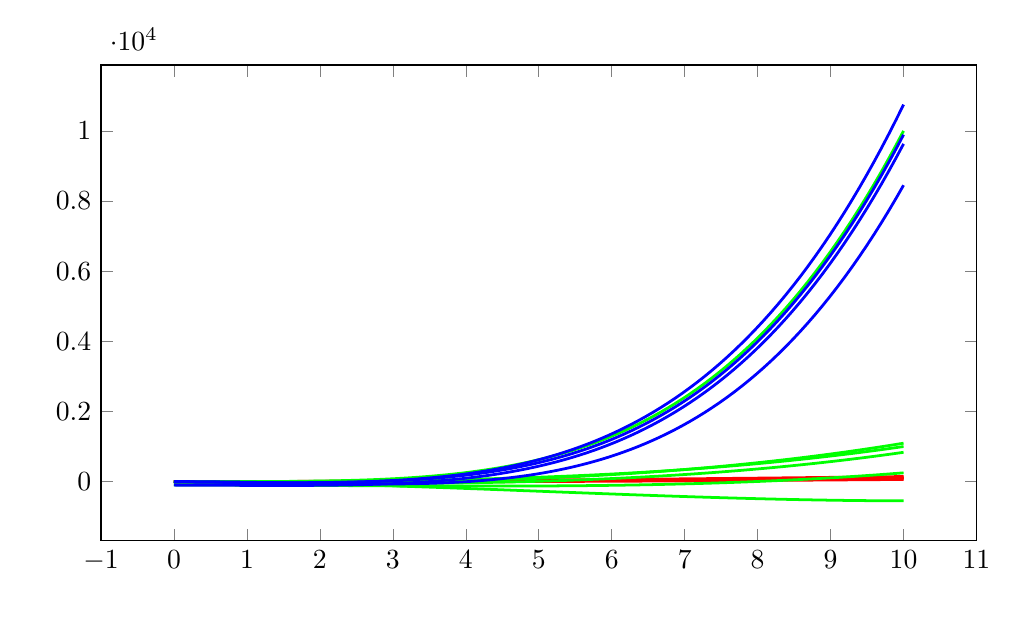
\begin{tikzpicture}[line width=1]
\begin{axis}[width=5in, height=3in,
             scatter/classes={a={mark=*,draw=black}},
             xlabel={\mbox{}},
             xlabel style={name=xlabel}, 
             ylabel={\mbox{}}, 
             legend style={
                at={(xlabel.south)},
                yshift=-1ex,
                anchor=north,
                legend cell align=left,
                },
        ]
]
\addplot[draw=red, line width=1] coordinates {(0.0,0.0)
(0.101,0.0102)
(0.202,0.0408)
(0.303,0.0918)
(0.404,0.1632)
(0.5051,0.2551)
(0.6061,0.3673)
(0.7071,0.4999)
(0.8081,0.653)
(0.9091,0.8264)
(1.0101,1.0203)
(1.1111,1.2346)
(1.2121,1.4692)
(1.3131,1.7243)
(1.4141,1.9998)
(1.5152,2.2957)
(1.6162,2.612)
(1.7172,2.9487)
(1.8182,3.3058)
(1.9192,3.6833)
(2.0202,4.0812)
(2.1212,4.4995)
(2.2222,4.9383)
(2.3232,5.3974)
(2.4242,5.877)
(2.5253,6.3769)
(2.6263,6.8973)
(2.7273,7.438)
(2.8283,7.9992)
(2.9293,8.5808)
(3.0303,9.1827)
(3.1313,9.8051)
(3.2323,10.4479)
(3.3333,11.1111)
(3.4343,11.7947)
(3.5354,12.4987)
(3.6364,13.2231)
(3.7374,13.968)
(3.8384,14.7332)
(3.9394,15.5188)
(4.0404,16.3249)
(4.1414,17.1513)
(4.2424,17.9982)
(4.3434,18.8654)
(4.4444,19.7531)
(4.5455,20.6612)
(4.6465,21.5896)
(4.7475,22.5385)
(4.8485,23.5078)
(4.9495,24.4975)
(5.0505,25.5076)
(5.1515,26.5381)
(5.2525,27.589)
(5.3535,28.6603)
(5.4545,29.7521)
(5.5556,30.8642)
(5.6566,31.9967)
(5.7576,33.1497)
(5.8586,34.323)
(5.9596,35.5168)
(6.0606,36.7309)
(6.1616,37.9655)
(6.2626,39.2205)
(6.3636,40.4959)
(6.4646,41.7917)
(6.5657,43.1078)
(6.6667,44.4444)
(6.7677,45.8014)
(6.8687,47.1789)
(6.9697,48.5767)
(7.0707,49.9949)
(7.1717,51.4335)
(7.2727,52.8926)
(7.3737,54.372)
(7.4747,55.8718)
(7.5758,57.3921)
(7.6768,58.9328)
(7.7778,60.4938)
(7.8788,62.0753)
(7.9798,63.6772)
(8.0808,65.2995)
(8.1818,66.9421)
(8.2828,68.6052)
(8.3838,70.2887)
(8.4848,71.9927)
(8.5859,73.717)
(8.6869,75.4617)
(8.7879,77.2268)
(8.8889,79.0123)
(8.9899,80.8183)
(9.0909,82.6446)
(9.1919,84.4914)
(9.2929,86.3585)
(9.3939,88.2461)
(9.4949,90.1541)
(9.596,92.0824)
(9.697,94.0312)
(9.798,96.0004)
(9.899,97.99)
(10.0,100.0)
(10.0,100.0)};\addplot[draw=red, line width=1] coordinates {(0.0,2.0)
(0.101,2.0102)
(0.202,2.0408)
(0.303,2.0918)
(0.404,2.1632)
(0.5051,2.2551)
(0.6061,2.3673)
(0.7071,2.4999)
(0.8081,2.653)
(0.9091,2.8264)
(1.0101,3.0203)
(1.1111,3.2346)
(1.2121,3.4692)
(1.3131,3.7243)
(1.4141,3.9998)
(1.5152,4.2957)
(1.6162,4.612)
(1.7172,4.9487)
(1.8182,5.3058)
(1.9192,5.6833)
(2.0202,6.0812)
(2.1212,6.4995)
(2.2222,6.9383)
(2.3232,7.3974)
(2.4242,7.877)
(2.5253,8.3769)
(2.6263,8.8973)
(2.7273,9.438)
(2.8283,9.9992)
(2.9293,10.5808)
(3.0303,11.1827)
(3.1313,11.8051)
(3.2323,12.4479)
(3.3333,13.1111)
(3.4343,13.7947)
(3.5354,14.4987)
(3.6364,15.2231)
(3.7374,15.968)
(3.8384,16.7332)
(3.9394,17.5188)
(4.0404,18.3249)
(4.1414,19.1513)
(4.2424,19.9982)
(4.3434,20.8654)
(4.4444,21.7531)
(4.5455,22.6612)
(4.6465,23.5896)
(4.7475,24.5385)
(4.8485,25.5078)
(4.9495,26.4975)
(5.0505,27.5076)
(5.1515,28.5381)
(5.2525,29.589)
(5.3535,30.6603)
(5.4545,31.7521)
(5.5556,32.8642)
(5.6566,33.9967)
(5.7576,35.1497)
(5.8586,36.323)
(5.9596,37.5168)
(6.0606,38.7309)
(6.1616,39.9655)
(6.2626,41.2205)
(6.3636,42.4959)
(6.4646,43.7917)
(6.5657,45.1078)
(6.6667,46.4444)
(6.7677,47.8014)
(6.8687,49.1789)
(6.9697,50.5767)
(7.0707,51.9949)
(7.1717,53.4335)
(7.2727,54.8926)
(7.3737,56.372)
(7.4747,57.8718)
(7.5758,59.3921)
(7.6768,60.9328)
(7.7778,62.4938)
(7.8788,64.0753)
(7.9798,65.6772)
(8.0808,67.2995)
(8.1818,68.9421)
(8.2828,70.6052)
(8.3838,72.2887)
(8.4848,73.9927)
(8.5859,75.717)
(8.6869,77.4617)
(8.7879,79.2268)
(8.8889,81.0123)
(8.9899,82.8183)
(9.0909,84.6446)
(9.1919,86.4914)
(9.2929,88.3585)
(9.3939,90.2461)
(9.4949,92.1541)
(9.596,94.0824)
(9.697,96.0312)
(9.798,98.0004)
(9.899,99.99)
(10.0,102.0)
(10.0,102.0)};\addplot[draw=red, line width=1] coordinates {(0.0,1.0)
(0.101,1.0102)
(0.202,1.0408)
(0.303,1.0918)
(0.404,1.1632)
(0.5051,1.2551)
(0.6061,1.3673)
(0.7071,1.4999)
(0.8081,1.653)
(0.9091,1.8264)
(1.0101,2.0203)
(1.1111,2.2346)
(1.2121,2.4692)
(1.3131,2.7243)
(1.4141,2.9998)
(1.5152,3.2957)
(1.6162,3.612)
(1.7172,3.9487)
(1.8182,4.3058)
(1.9192,4.6833)
(2.0202,5.0812)
(2.1212,5.4995)
(2.2222,5.9383)
(2.3232,6.3974)
(2.4242,6.877)
(2.5253,7.3769)
(2.6263,7.8973)
(2.7273,8.438)
(2.8283,8.9992)
(2.9293,9.5808)
(3.0303,10.1827)
(3.1313,10.8051)
(3.2323,11.4479)
(3.3333,12.1111)
(3.4343,12.7947)
(3.5354,13.4987)
(3.6364,14.2231)
(3.7374,14.968)
(3.8384,15.7332)
(3.9394,16.5188)
(4.0404,17.3249)
(4.1414,18.1513)
(4.2424,18.9982)
(4.3434,19.8654)
(4.4444,20.7531)
(4.5455,21.6612)
(4.6465,22.5896)
(4.7475,23.5385)
(4.8485,24.5078)
(4.9495,25.4975)
(5.0505,26.5076)
(5.1515,27.5381)
(5.2525,28.589)
(5.3535,29.6603)
(5.4545,30.7521)
(5.5556,31.8642)
(5.6566,32.9967)
(5.7576,34.1497)
(5.8586,35.323)
(5.9596,36.5168)
(6.0606,37.7309)
(6.1616,38.9655)
(6.2626,40.2205)
(6.3636,41.4959)
(6.4646,42.7917)
(6.5657,44.1078)
(6.6667,45.4444)
(6.7677,46.8014)
(6.8687,48.1789)
(6.9697,49.5767)
(7.0707,50.9949)
(7.1717,52.4335)
(7.2727,53.8926)
(7.3737,55.372)
(7.4747,56.8718)
(7.5758,58.3921)
(7.6768,59.9328)
(7.7778,61.4938)
(7.8788,63.0753)
(7.9798,64.6772)
(8.0808,66.2995)
(8.1818,67.9421)
(8.2828,69.6052)
(8.3838,71.2887)
(8.4848,72.9927)
(8.5859,74.717)
(8.6869,76.4617)
(8.7879,78.2268)
(8.8889,80.0123)
(8.9899,81.8183)
(9.0909,83.6446)
(9.1919,85.4914)
(9.2929,87.3585)
(9.3939,89.2461)
(9.4949,91.1541)
(9.596,93.0824)
(9.697,95.0312)
(9.798,97.0004)
(9.899,98.99)
(10.0,101.0)
(10.0,101.0)};\addplot[draw=red, line width=1] coordinates {(0.0,-5.0)
(0.101,-4.4847)
(0.202,-3.9491)
(0.303,-3.393)
(0.404,-2.8165)
(0.5051,-2.2197)
(0.6061,-1.6024)
(0.7071,-0.9647)
(0.8081,-0.3066)
(0.9091,0.3719)
(1.0101,1.0708)
(1.1111,1.7901)
(1.2121,2.5298)
(1.3131,3.29)
(1.4141,4.0705)
(1.5152,4.8714)
(1.6162,5.6928)
(1.7172,6.5345)
(1.8182,7.3967)
(1.9192,8.2793)
(2.0202,9.1822)
(2.1212,10.1056)
(2.2222,11.0494)
(2.3232,12.0136)
(2.4242,12.9982)
(2.5253,14.0032)
(2.6263,15.0286)
(2.7273,16.0744)
(2.8283,17.1406)
(2.9293,18.2272)
(3.0303,19.3343)
(3.1313,20.4617)
(3.2323,21.6095)
(3.3333,22.7778)
(3.4343,23.9664)
(3.5354,25.1755)
(3.6364,26.405)
(3.7374,27.6548)
(3.8384,28.9251)
(3.9394,30.2158)
(4.0404,31.5269)
(4.1414,32.8584)
(4.2424,34.2103)
(4.3434,35.5826)
(4.4444,36.9753)
(4.5455,38.3884)
(4.6465,39.822)
(4.7475,41.2759)
(4.8485,42.7502)
(4.9495,44.245)
(5.0505,45.7601)
(5.1515,47.2957)
(5.2525,48.8516)
(5.3535,50.428)
(5.4545,52.0248)
(5.5556,53.642)
(5.6566,55.2796)
(5.7576,56.9376)
(5.8586,58.616)
(5.9596,60.3148)
(6.0606,62.034)
(6.1616,63.7736)
(6.2626,65.5336)
(6.3636,67.314)
(6.4646,69.1149)
(6.5657,70.9361)
(6.6667,72.7778)
(6.7677,74.6398)
(6.8687,76.5223)
(6.9697,78.4252)
(7.0707,80.3484)
(7.1717,82.2921)
(7.2727,84.2562)
(7.3737,86.2407)
(7.4747,88.2456)
(7.5758,90.2709)
(7.6768,92.3166)
(7.7778,94.3827)
(7.8788,96.4692)
(7.9798,98.5762)
(8.0808,100.7035)
(8.1818,102.8512)
(8.2828,105.0194)
(8.3838,107.2079)
(8.4848,109.4169)
(8.5859,111.6463)
(8.6869,113.896)
(8.7879,116.1662)
(8.8889,118.4568)
(8.9899,120.7678)
(9.0909,123.0992)
(9.1919,125.451)
(9.2929,127.8232)
(9.3939,130.2158)
(9.4949,132.6288)
(9.596,135.0622)
(9.697,137.5161)
(9.798,139.9903)
(9.899,142.485)
(10.0,145.0)
(10.0,145.0)};\addplot[draw=red, line width=1] coordinates {(0.0,-8.0)
(0.101,-8.2928)
(0.202,-8.5652)
(0.303,-8.8173)
(0.404,-9.0489)
(0.5051,-9.2601)
(0.6061,-9.4509)
(0.7071,-9.6213)
(0.8081,-9.7712)
(0.9091,-9.9008)
(1.0101,-10.01)
(1.1111,-10.0988)
(1.2121,-10.1671)
(1.3131,-10.2151)
(1.4141,-10.2426)
(1.5152,-10.2498)
(1.6162,-10.2365)
(1.7172,-10.2028)
(1.8182,-10.1488)
(1.9192,-10.0743)
(2.0202,-9.9794)
(2.1212,-9.8641)
(2.2222,-9.7284)
(2.3232,-9.5723)
(2.4242,-9.3958)
(2.5253,-9.1989)
(2.6263,-8.9815)
(2.7273,-8.7438)
(2.8283,-8.4857)
(2.9293,-8.2071)
(3.0303,-7.9082)
(3.1313,-7.5888)
(3.2323,-7.2491)
(3.3333,-6.8889)
(3.4343,-6.5083)
(3.5354,-6.1073)
(3.6364,-5.686)
(3.7374,-5.2442)
(3.8384,-4.782)
(3.9394,-4.2994)
(4.0404,-3.7963)
(4.1414,-3.2729)
(4.2424,-2.7291)
(4.3434,-2.1649)
(4.4444,-1.5802)
(4.5455,-0.9752)
(4.6465,-0.3498)
(4.7475,0.2961)
(4.8485,0.9624)
(4.9495,1.649)
(5.0505,2.3561)
(5.1515,3.0836)
(5.2525,3.8314)
(5.3535,4.5997)
(5.4545,5.3884)
(5.5556,6.1975)
(5.6566,7.027)
(5.7576,7.877)
(5.8586,8.7473)
(5.9596,9.638)
(6.0606,10.5491)
(6.1616,11.4807)
(6.2626,12.4326)
(6.3636,13.405)
(6.4646,14.3977)
(6.5657,15.4109)
(6.6667,16.4444)
(6.7677,17.4984)
(6.8687,18.5728)
(6.9697,19.6676)
(7.0707,20.7828)
(7.1717,21.9184)
(7.2727,23.0744)
(7.3737,24.2508)
(7.4747,25.4476)
(7.5758,26.6648)
(7.6768,27.9025)
(7.7778,29.1605)
(7.8788,30.4389)
(7.9798,31.7378)
(8.0808,33.057)
(8.1818,34.3967)
(8.2828,35.7568)
(8.3838,37.1372)
(8.4848,38.5381)
(8.5859,39.9594)
(8.6869,41.4011)
(8.7879,42.8632)
(8.8889,44.3457)
(8.9899,45.8486)
(9.0909,47.3719)
(9.1919,48.9156)
(9.2929,50.4797)
(9.3939,52.0643)
(9.4949,53.6692)
(9.596,55.2946)
(9.697,56.9403)
(9.798,58.6065)
(9.899,60.293)
(10.0,62.0)
(10.0,62.0)};\addplot[draw=green, line width=1] coordinates {(0.0,0.0)
(0.101,0.001)
(0.202,0.0082)
(0.303,0.0278)
(0.404,0.066)
(0.5051,0.1288)
(0.6061,0.2226)
(0.7071,0.3535)
(0.8081,0.5277)
(0.9091,0.7513)
(1.0101,1.0306)
(1.1111,1.3717)
(1.2121,1.7809)
(1.3131,2.2643)
(1.4141,2.828)
(1.5152,3.4783)
(1.6162,4.2214)
(1.7172,5.0634)
(1.8182,6.0105)
(1.9192,7.069)
(2.0202,8.2449)
(2.1212,9.5445)
(2.2222,10.9739)
(2.3232,12.5394)
(2.4242,14.2472)
(2.5253,16.1033)
(2.6263,18.114)
(2.7273,20.2855)
(2.8283,22.624)
(2.9293,25.1356)
(3.0303,27.8265)
(3.1313,30.7029)
(3.2323,33.771)
(3.3333,37.037)
(3.4343,40.5071)
(3.5354,44.1874)
(3.6364,48.0841)
(3.7374,52.2035)
(3.8384,56.5516)
(3.9394,61.1348)
(4.0404,65.959)
(4.1414,71.0307)
(4.2424,76.3558)
(4.3434,81.9407)
(4.4444,87.7915)
(4.5455,93.9144)
(4.6465,100.3155)
(4.7475,107.001)
(4.8485,113.9772)
(4.9495,121.2503)
(5.0505,128.8263)
(5.1515,136.7115)
(5.2525,144.912)
(5.3535,153.4341)
(5.4545,162.284)
(5.5556,171.4678)
(5.6566,180.9916)
(5.7576,190.8618)
(5.8586,201.0844)
(5.9596,211.6657)
(6.0606,222.6118)
(6.1616,233.9289)
(6.2626,245.6233)
(6.3636,257.701)
(6.4646,270.1683)
(6.5657,283.0313)
(6.6667,296.2963)
(6.7677,309.9694)
(6.8687,324.0568)
(6.9697,338.5647)
(7.0707,353.4993)
(7.1717,368.8667)
(7.2727,384.6732)
(7.3737,400.9249)
(7.4747,417.628)
(7.5758,434.7887)
(7.6768,452.4131)
(7.7778,470.5075)
(7.8788,489.0781)
(7.9798,508.131)
(8.0808,527.6724)
(8.1818,547.7085)
(8.2828,568.2455)
(8.3838,589.2895)
(8.4848,610.8468)
(8.5859,632.9235)
(8.6869,655.5258)
(8.7879,678.6599)
(8.8889,702.332)
(8.9899,726.5482)
(9.0909,751.3148)
(9.1919,776.6379)
(9.2929,802.5238)
(9.3939,828.9785)
(9.4949,856.0083)
(9.596,883.6194)
(9.697,911.8179)
(9.798,940.6101)
(9.899,970.002)
(10.0,1000.0)
(10.0,1000.0)};\addplot[draw=green, line width=1] coordinates {(0.0,-5.0)
(0.101,-6.9886)
(0.202,-8.9097)
(0.303,-10.7573)
(0.404,-12.5251)
(0.5051,-14.207)
(0.6061,-15.7967)
(0.7071,-17.2881)
(0.8081,-18.675)
(0.9091,-19.9512)
(1.0101,-21.1105)
(1.1111,-22.1468)
(1.2121,-23.0538)
(1.3131,-23.8254)
(1.4141,-24.4554)
(1.5152,-24.9377)
(1.6162,-25.2659)
(1.7172,-25.434)
(1.8182,-25.4358)
(1.9192,-25.265)
(2.0202,-24.9155)
(2.1212,-24.3811)
(2.2222,-23.6557)
(2.3232,-22.733)
(2.4242,-21.6068)
(2.5253,-20.2711)
(2.6263,-18.7195)
(2.7273,-16.9459)
(2.8283,-14.9442)
(2.9293,-12.708)
(3.0303,-10.2314)
(3.1313,-7.508)
(3.2323,-4.5317)
(3.3333,-1.2963)
(3.4343,2.2044)
(3.5354,5.9765)
(3.6364,10.0263)
(3.7374,14.3599)
(3.8384,18.9835)
(3.9394,23.9034)
(4.0404,29.1256)
(4.1414,34.6563)
(4.2424,40.5019)
(4.3434,46.6683)
(4.4444,53.1619)
(4.5455,59.9887)
(4.6465,67.1551)
(4.7475,74.6671)
(4.8485,82.531)
(4.9495,90.7529)
(5.0505,99.339)
(5.1515,108.2955)
(5.2525,117.6286)
(5.3535,127.3445)
(5.4545,137.4493)
(5.5556,147.9492)
(5.6566,158.8505)
(5.7576,170.1593)
(5.8586,181.8818)
(5.9596,194.0241)
(6.0606,206.5925)
(6.1616,219.5931)
(6.2626,233.0322)
(6.3636,246.9159)
(6.4646,261.2503)
(6.5657,276.0417)
(6.6667,291.2963)
(6.7677,307.0202)
(6.8687,323.2197)
(6.9697,339.9008)
(7.0707,357.0698)
(7.1717,374.7329)
(7.2727,392.8963)
(7.3737,411.5661)
(7.4747,430.7486)
(7.5758,450.4498)
(7.6768,470.6761)
(7.7778,491.4335)
(7.8788,512.7282)
(7.9798,534.5666)
(8.0808,556.9546)
(8.1818,579.8986)
(8.2828,603.4046)
(8.3838,627.479)
(8.4848,652.1278)
(8.5859,677.3572)
(8.6869,703.1735)
(8.7879,729.5827)
(8.8889,756.5912)
(8.9899,784.2051)
(9.0909,812.4305)
(9.1919,841.2737)
(9.2929,870.7408)
(9.3939,900.838)
(9.4949,931.5715)
(9.596,962.9475)
(9.697,994.9722)
(9.798,1027.6517)
(9.899,1060.9922)
(10.0,1095.0)
(10.0,1095.0)};\addplot[draw=green, line width=1] coordinates {(0.0,-15.0)
(0.101,-17.514)
(0.202,-20.0014)
(0.303,-22.4561)
(0.404,-24.8718)
(0.5051,-27.2424)
(0.6061,-29.5616)
(0.7071,-31.8233)
(0.8081,-34.0214)
(0.9091,-36.1495)
(1.0101,-38.2016)
(1.1111,-40.1715)
(1.2121,-42.0529)
(1.3131,-43.8397)
(1.4141,-45.5257)
(1.5152,-47.1048)
(1.6162,-48.5707)
(1.7172,-49.9172)
(1.8182,-51.1382)
(1.9192,-52.2275)
(2.0202,-53.179)
(2.1212,-53.9863)
(2.2222,-54.6433)
(2.3232,-55.144)
(2.4242,-55.482)
(2.5253,-55.6511)
(2.6263,-55.6453)
(2.7273,-55.4583)
(2.8283,-55.0839)
(2.9293,-54.516)
(3.0303,-53.7484)
(3.1313,-52.7748)
(3.2323,-51.5891)
(3.3333,-50.1852)
(3.4343,-48.5568)
(3.5354,-46.6977)
(3.6364,-44.6018)
(3.7374,-42.2629)
(3.8384,-39.6748)
(3.9394,-36.8313)
(4.0404,-33.7262)
(4.1414,-30.3534)
(4.2424,-26.7066)
(4.3434,-22.7797)
(4.4444,-18.5665)
(4.5455,-14.0609)
(4.6465,-9.2565)
(4.7475,-4.1473)
(4.8485,1.2729)
(4.9495,7.0104)
(5.0505,13.0712)
(5.1515,19.4617)
(5.2525,26.1879)
(5.3535,33.2561)
(5.4545,40.6724)
(5.5556,48.4431)
(5.6566,56.5742)
(5.7576,65.0721)
(5.8586,73.9428)
(5.9596,83.1926)
(6.0606,92.8276)
(6.1616,102.854)
(6.2626,113.2781)
(6.3636,124.1059)
(6.4646,135.3438)
(6.5657,146.9977)
(6.6667,159.0741)
(6.7677,171.5789)
(6.8687,184.5185)
(6.9697,197.899)
(7.0707,211.7265)
(7.1717,226.0073)
(7.2727,240.7476)
(7.3737,255.9534)
(7.4747,271.6311)
(7.5758,287.7868)
(7.6768,304.4267)
(7.7778,321.5569)
(7.8788,339.1837)
(7.9798,357.3132)
(8.0808,375.9517)
(8.1818,395.1052)
(8.2828,414.78)
(8.3838,434.9823)
(8.4848,455.7182)
(8.5859,476.994)
(8.6869,498.8157)
(8.7879,521.1897)
(8.8889,544.1221)
(8.9899,567.619)
(9.0909,591.6867)
(9.1919,616.3313)
(9.2929,641.5591)
(9.3939,667.3761)
(9.4949,693.7886)
(9.596,720.8028)
(9.697,748.4249)
(9.798,776.661)
(9.899,805.5173)
(10.0,835.0)
(10.0,835.0)};\addplot[draw=green, line width=1] coordinates {(0.0,1.0)
(0.101,0.3429)
(0.202,-0.614)
(0.303,-1.8647)
(0.404,-3.403)
(0.5051,-5.2226)
(0.6061,-7.3173)
(0.7071,-9.6811)
(0.8081,-12.3077)
(0.9091,-15.1908)
(1.0101,-18.3245)
(1.1111,-21.7023)
(1.2121,-25.3183)
(1.3131,-29.1661)
(1.4141,-33.2397)
(1.5152,-37.5327)
(1.6162,-42.0391)
(1.7172,-46.7527)
(1.8182,-51.6672)
(1.9192,-56.7765)
(2.0202,-62.0744)
(2.1212,-67.5547)
(2.2222,-73.2112)
(2.3232,-79.0379)
(2.4242,-85.0283)
(2.5253,-91.1765)
(2.6263,-97.4761)
(2.7273,-103.9211)
(2.8283,-110.5052)
(2.9293,-117.2223)
(3.0303,-124.0661)
(3.1313,-131.0305)
(3.2323,-138.1093)
(3.3333,-145.2963)
(3.4343,-152.5853)
(3.5354,-159.9702)
(3.6364,-167.4448)
(3.7374,-175.0028)
(3.8384,-182.6381)
(3.9394,-190.3446)
(4.0404,-198.1159)
(4.1414,-205.9461)
(4.2424,-213.8287)
(4.3434,-221.7578)
(4.4444,-229.727)
(4.5455,-237.7303)
(4.6465,-245.7614)
(4.7475,-253.8141)
(4.8485,-261.8823)
(4.9495,-269.9597)
(5.0505,-278.0403)
(5.1515,-286.1177)
(5.2525,-294.1859)
(5.3535,-302.2386)
(5.4545,-310.2697)
(5.5556,-318.273)
(5.6566,-326.2422)
(5.7576,-334.1713)
(5.8586,-342.0539)
(5.9596,-349.8841)
(6.0606,-357.6554)
(6.1616,-365.3619)
(6.2626,-372.9972)
(6.3636,-380.5552)
(6.4646,-388.0298)
(6.5657,-395.4147)
(6.6667,-402.7037)
(6.7677,-409.8907)
(6.8687,-416.9695)
(6.9697,-423.9339)
(7.0707,-430.7777)
(7.1717,-437.4948)
(7.2727,-444.0789)
(7.3737,-450.5239)
(7.4747,-456.8235)
(7.5758,-462.9717)
(7.6768,-468.9621)
(7.7778,-474.7888)
(7.8788,-480.4453)
(7.9798,-485.9256)
(8.0808,-491.2235)
(8.1818,-496.3328)
(8.2828,-501.2473)
(8.3838,-505.9609)
(8.4848,-510.4673)
(8.5859,-514.7603)
(8.6869,-518.8339)
(8.7879,-522.6817)
(8.8889,-526.2977)
(8.9899,-529.6755)
(9.0909,-532.8092)
(9.1919,-535.6923)
(9.2929,-538.3189)
(9.3939,-540.6827)
(9.4949,-542.7774)
(9.596,-544.597)
(9.697,-546.1353)
(9.798,-547.386)
(9.899,-548.3429)
(10.0,-549.0)
(10.0,-549.0)};\addplot[draw=green, line width=1] coordinates {(0.0,-100.0)
(0.101,-99.5653)
(0.202,-99.2673)
(0.303,-99.0998)
(0.404,-99.0566)
(0.5051,-99.1315)
(0.6061,-99.3183)
(0.7071,-99.6108)
(0.8081,-100.0029)
(0.9091,-100.4884)
(1.0101,-101.061)
(1.1111,-101.7147)
(1.2121,-102.4432)
(1.3131,-103.2403)
(1.4141,-104.0999)
(1.5152,-105.0157)
(1.6162,-105.9817)
(1.7172,-106.9915)
(1.8182,-108.0391)
(1.9192,-109.1182)
(2.0202,-110.2226)
(2.1212,-111.3462)
(2.2222,-112.4829)
(2.3232,-113.6263)
(2.4242,-114.7703)
(2.5253,-115.9088)
(2.6263,-117.0355)
(2.7273,-118.1443)
(2.8283,-119.2289)
(2.9293,-120.2833)
(3.0303,-121.3012)
(3.1313,-122.2764)
(3.2323,-123.2027)
(3.3333,-124.0741)
(3.4343,-124.8842)
(3.5354,-125.6269)
(3.6364,-126.296)
(3.7374,-126.8854)
(3.8384,-127.3888)
(3.9394,-127.8)
(4.0404,-128.113)
(4.1414,-128.3214)
(4.2424,-128.4192)
(4.3434,-128.4001)
(4.4444,-128.2579)
(4.5455,-127.9865)
(4.6465,-127.5796)
(4.7475,-127.0312)
(4.8485,-126.335)
(4.9495,-125.4848)
(5.0505,-124.4744)
(5.1515,-123.2977)
(5.2525,-121.9485)
(5.3535,-120.4206)
(5.4545,-118.7077)
(5.5556,-116.8038)
(5.6566,-114.7027)
(5.7576,-112.3981)
(5.8586,-109.8839)
(5.9596,-107.1538)
(6.0606,-104.2018)
(6.1616,-101.0216)
(6.2626,-97.607)
(6.3636,-93.9519)
(6.4646,-90.0501)
(6.5657,-85.8953)
(6.6667,-81.4815)
(6.7677,-76.8024)
(6.8687,-71.8518)
(6.9697,-66.6235)
(7.0707,-61.1115)
(7.1717,-55.3094)
(7.2727,-49.2111)
(7.3737,-42.8105)
(7.4747,-36.1012)
(7.5758,-29.0773)
(7.6768,-21.7324)
(7.7778,-14.0604)
(7.8788,-6.055)
(7.9798,2.2898)
(8.0808,10.9802)
(8.1818,20.0225)
(8.2828,29.4229)
(8.3838,39.1875)
(8.4848,49.3224)
(8.5859,59.834)
(8.6869,70.7283)
(8.7879,82.0116)
(8.8889,93.69)
(8.9899,105.7697)
(9.0909,118.2569)
(9.1919,131.1579)
(9.2929,144.4787)
(9.3939,158.2255)
(9.4949,172.4046)
(9.596,187.0221)
(9.697,202.0842)
(9.798,217.5971)
(9.899,233.567)
(10.0,250.0)
(10.0,250.0)};\addplot[draw=green, line width=1] coordinates {(0.0,0.0)
(0.101,0.0001)
(0.202,0.0017)
(0.303,0.0084)
(0.404,0.0267)
(0.5051,0.0651)
(0.6061,0.1349)
(0.7071,0.2499)
(0.8081,0.4264)
(0.9091,0.683)
(1.0101,1.041)
(1.1111,1.5242)
(1.2121,2.1587)
(1.3131,2.9733)
(1.4141,3.9992)
(1.5152,5.2702)
(1.6162,6.8224)
(1.7172,8.6947)
(1.8182,10.9282)
(1.9192,13.5667)
(2.0202,16.6563)
(2.1212,20.2459)
(2.2222,24.3865)
(2.3232,29.132)
(2.4242,34.5386)
(2.5253,40.6649)
(2.6263,47.5721)
(2.7273,55.3241)
(2.8283,63.9869)
(2.9293,73.6294)
(3.0303,84.3226)
(3.1313,96.1404)
(3.2323,109.1589)
(3.3333,123.4568)
(3.4343,139.1153)
(3.5354,156.2181)
(3.6364,174.8514)
(3.7374,195.104)
(3.8384,217.0669)
(3.9394,240.8339)
(4.0404,266.5012)
(4.1414,294.1675)
(4.2424,323.9339)
(4.3434,355.9041)
(4.4444,390.1844)
(4.5455,426.8834)
(4.6465,466.1123)
(4.7475,507.9847)
(4.8485,552.6169)
(4.9495,600.1275)
(5.0505,650.6377)
(5.1515,704.2712)
(5.2525,761.1541)
(5.3535,821.4151)
(5.4545,885.1854)
(5.5556,952.5987)
(5.6566,1023.7911)
(5.7576,1098.9012)
(5.8586,1178.0703)
(5.9596,1261.4419)
(6.0606,1349.1624)
(6.1616,1441.3802)
(6.2626,1538.2467)
(6.3636,1639.9153)
(6.4646,1746.5423)
(6.5657,1858.2864)
(6.6667,1975.3086)
(6.7677,2097.7727)
(6.8687,2225.8448)
(6.9697,2359.6934)
(7.0707,2499.4899)
(7.1717,2645.4077)
(7.2727,2797.6231)
(7.3737,2956.3147)
(7.4747,3121.6636)
(7.5758,3293.8535)
(7.6768,3473.0704)
(7.7778,3659.5031)
(7.8788,3853.3427)
(7.9798,4054.7827)
(8.0808,4264.0194)
(8.1818,4481.2513)
(8.2828,4706.6796)
(8.3838,4940.5078)
(8.4848,5182.9422)
(8.5859,5434.1913)
(8.6869,5694.4663)
(8.7879,5963.9807)
(8.8889,6242.9508)
(8.9899,6531.595)
(9.0909,6830.1346)
(9.1919,7138.793)
(9.2929,7457.7965)
(9.3939,7787.3737)
(9.4949,8127.7556)
(9.596,8479.1759)
(9.697,8841.8706)
(9.798,9216.0784)
(9.899,9602.0403)
(10.0,10000.0)
(10.0,10000.0)};\addplot[draw=blue, line width=1] coordinates {(0.0,-9.0)
(0.101,-11.0099)
(0.202,-12.9979)
(0.303,-14.9603)
(0.404,-16.8909)
(0.5051,-18.7809)
(0.6061,-20.619)
(0.7071,-22.3915)
(0.8081,-24.0822)
(0.9091,-25.6724)
(1.0101,-27.1407)
(1.1111,-28.4635)
(1.2121,-29.6145)
(1.3131,-30.5651)
(1.4141,-31.2838)
(1.5152,-31.7372)
(1.6162,-31.8888)
(1.7172,-31.7)
(1.8182,-31.1296)
(1.9192,-30.1339)
(2.0202,-28.6665)
(2.1212,-26.6788)
(2.2222,-24.1196)
(2.3232,-20.9352)
(2.4242,-17.0693)
(2.5253,-12.4633)
(2.6263,-7.0559)
(2.7273,-0.7833)
(2.8283,6.4205)
(2.9293,14.6243)
(3.0303,23.8993)
(3.1313,34.3193)
(3.2323,45.9603)
(3.3333,58.9012)
(3.4343,73.2231)
(3.5354,89.0098)
(3.6364,106.3473)
(3.7374,125.3245)
(3.8384,146.0324)
(3.9394,168.5649)
(4.0404,193.018)
(4.1414,219.4905)
(4.2424,248.0836)
(4.3434,278.9009)
(4.4444,312.0486)
(4.5455,347.6355)
(4.6465,385.7726)
(4.7475,426.5737)
(4.8485,470.155)
(4.9495,516.6351)
(5.0505,566.1352)
(5.1515,618.779)
(5.2525,674.6926)
(5.3535,734.0048)
(5.4545,796.8466)
(5.5556,863.3518)
(5.6566,933.6565)
(5.7576,1007.8994)
(5.8586,1086.2216)
(5.9596,1168.7668)
(6.0606,1255.6812)
(6.1616,1347.1134)
(6.2626,1443.2146)
(6.3636,1544.1384)
(6.4646,1650.0411)
(6.5657,1761.0811)
(6.6667,1877.4198)
(6.7677,1999.2206)
(6.8687,2126.6499)
(6.9697,2259.8762)
(7.0707,2399.0706)
(7.1717,2544.4069)
(7.2727,2696.0611)
(7.3737,2854.212)
(7.4747,3019.0405)
(7.5758,3190.7304)
(7.6768,3369.4678)
(7.7778,3555.4414)
(7.8788,3748.8422)
(7.9798,3949.8639)
(8.0808,4158.7027)
(8.1818,4375.5571)
(8.2828,4600.6282)
(8.3838,4834.1198)
(8.4848,5076.2379)
(8.5859,5327.1911)
(8.6869,5587.1906)
(8.7879,5856.45)
(8.8889,6135.1853)
(8.9899,6423.6153)
(9.0909,6721.961)
(9.1919,7030.446)
(9.2929,7349.2965)
(9.3939,7678.741)
(9.4949,8019.0107)
(9.596,8370.3391)
(9.697,8732.9624)
(9.798,9107.1192)
(9.899,9493.0505)
(10.0,9891.0)
(10.0,9891.0)};\addplot[draw=blue, line width=1] coordinates {(0.0,-1.0)
(0.101,-3.5241)
(0.202,-6.0406)
(0.303,-8.5395)
(0.404,-11.0084)
(0.5051,-13.4324)
(0.6061,-15.794)
(0.7071,-18.0733)
(0.8081,-20.2479)
(0.9091,-22.2929)
(1.0101,-24.1809)
(1.1111,-25.8819)
(1.2121,-27.3635)
(1.3131,-28.5908)
(1.4141,-29.5264)
(1.5152,-30.1303)
(1.6162,-30.3602)
(1.7172,-30.1712)
(1.8182,-29.5158)
(1.9192,-28.3442)
(2.0202,-26.6038)
(2.1212,-24.24)
(2.2222,-21.1951)
(2.3232,-17.4094)
(2.4242,-12.8203)
(2.5253,-7.3632)
(2.6263,-0.9704)
(2.7273,6.4278)
(2.8283,14.9038)
(2.9293,24.5326)
(3.0303,35.3915)
(3.1313,47.5605)
(3.2323,61.1218)
(3.3333,76.1605)
(3.4343,92.7638)
(3.5354,111.0217)
(3.6364,131.0265)
(3.7374,152.8731)
(3.8384,176.6589)
(3.9394,202.4838)
(4.0404,230.4502)
(4.1414,260.6628)
(4.2424,293.2291)
(4.3434,328.259)
(4.4444,365.8648)
(4.5455,406.1614)
(4.6465,449.2661)
(4.7475,495.2989)
(4.8485,544.382)
(4.9495,596.6404)
(5.0505,652.2014)
(5.1515,711.1948)
(5.2525,773.753)
(5.3535,840.0109)
(5.4545,910.1058)
(5.5556,984.1776)
(5.6566,1062.3685)
(5.7576,1144.8236)
(5.8586,1231.69)
(5.9596,1323.1177)
(6.0606,1419.259)
(6.1616,1520.2688)
(6.2626,1626.3043)
(6.3636,1737.5254)
(6.4646,1854.0944)
(6.5657,1976.1763)
(6.6667,2103.9383)
(6.7677,2237.5502)
(6.8687,2377.1844)
(6.9697,2523.0157)
(7.0707,2675.2215)
(7.1717,2833.9815)
(7.2727,2999.4781)
(7.3737,3171.8961)
(7.4747,3351.4229)
(7.5758,3538.2482)
(7.6768,3732.5644)
(7.7778,3934.5662)
(7.8788,4144.4511)
(7.9798,4362.4188)
(8.0808,4588.6716)
(8.1818,4823.4143)
(8.2828,5066.8543)
(8.3838,5319.2013)
(8.4848,5580.6678)
(8.5859,5851.4683)
(8.6869,6131.8203)
(8.7879,6421.9436)
(8.8889,6722.0605)
(8.9899,7032.3957)
(9.0909,7353.1766)
(9.1919,7684.633)
(9.2929,8026.9971)
(9.3939,8380.5037)
(9.4949,8745.3902)
(9.596,9121.8963)
(9.697,9510.2642)
(9.798,9910.7389)
(9.899,10323.5676)
(10.0,10749.0)
(10.0,10749.0)};\addplot[draw=blue, line width=1] coordinates {(0.0,1.0)
(0.101,0.342)
(0.202,-0.6206)
(0.303,-1.8841)
(0.404,-3.4423)
(0.5051,-5.2863)
(0.6061,-7.405)
(0.7071,-9.7846)
(0.8081,-12.4089)
(0.9091,-15.2591)
(1.0101,-18.314)
(1.1111,-21.5499)
(1.2121,-24.9405)
(1.3131,-28.4571)
(1.4141,-32.0685)
(1.5152,-35.7409)
(1.6162,-39.4381)
(1.7172,-43.1213)
(1.8182,-46.7495)
(1.9192,-50.2787)
(2.0202,-53.6629)
(2.1212,-56.8533)
(2.2222,-59.7987)
(2.3232,-62.4453)
(2.4242,-64.7369)
(2.5253,-66.6149)
(2.6263,-68.018)
(2.7273,-68.8825)
(2.8283,-69.1422)
(2.9293,-68.7284)
(3.0303,-67.5699)
(3.1313,-65.593)
(3.2323,-62.7214)
(3.3333,-58.8765)
(3.4343,-53.9771)
(3.5354,-47.9395)
(3.6364,-40.6775)
(3.7374,-32.1023)
(3.8384,-22.1229)
(3.9394,-10.6454)
(4.0404,2.4262)
(4.1414,17.1907)
(4.2424,33.7493)
(4.3434,52.2056)
(4.4444,72.6659)
(4.5455,95.2388)
(4.6465,120.0355)
(4.7475,147.1696)
(4.8485,176.7574)
(4.9495,208.9175)
(5.0505,243.7712)
(5.1515,281.442)
(5.2525,322.0562)
(5.3535,365.7423)
(5.4545,412.6317)
(5.5556,462.8579)
(5.6566,516.5572)
(5.7576,573.8681)
(5.8586,634.9319)
(5.9596,699.8922)
(6.0606,768.8952)
(6.1616,842.0894)
(6.2626,919.6262)
(6.3636,1001.6591)
(6.4646,1088.3443)
(6.5657,1179.8404)
(6.6667,1276.3086)
(6.7677,1377.9126)
(6.8687,1484.8184)
(6.9697,1597.1948)
(7.0707,1715.2129)
(7.1717,1839.0462)
(7.2727,1968.871)
(7.3737,2104.866)
(7.4747,2247.2121)
(7.5758,2396.0931)
(7.6768,2551.6952)
(7.7778,2714.2068)
(7.8788,2883.8193)
(7.9798,3060.7261)
(8.0808,3245.1234)
(8.1818,3437.21)
(8.2828,3637.1867)
(8.3838,3845.2574)
(8.4848,4061.6282)
(8.5859,4286.5075)
(8.6869,4520.1066)
(8.7879,4762.6391)
(8.8889,5014.3211)
(8.9899,5275.3713)
(9.0909,5546.0106)
(9.1919,5826.4628)
(9.2929,6116.9539)
(9.3939,6417.7125)
(9.4949,6728.9699)
(9.596,7050.9595)
(9.697,7383.9174)
(9.798,7728.0823)
(9.899,8083.6953)
(10.0,8451.0)
(10.0,8451.0)};\addplot[draw=blue, line width=1] coordinates {(0.0,-100.0)
(0.101,-100.7274)
(0.202,-101.4941)
(0.303,-102.2964)
(0.404,-103.1281)
(0.5051,-103.9804)
(0.6061,-104.8421)
(0.7071,-105.6994)
(0.8081,-106.5362)
(0.9091,-107.3335)
(1.0101,-108.0703)
(1.1111,-108.7228)
(1.2121,-109.2647)
(1.3131,-109.6673)
(1.4141,-109.8994)
(1.5152,-109.9273)
(1.6162,-109.7147)
(1.7172,-109.2229)
(1.8182,-108.4106)
(1.9192,-107.2343)
(2.0202,-105.6475)
(2.1212,-103.6017)
(2.2222,-101.0456)
(2.3232,-97.9254)
(2.4242,-94.185)
(2.5253,-89.7657)
(2.6263,-84.6062)
(2.7273,-78.6429)
(2.8283,-71.8094)
(2.9293,-64.0372)
(3.0303,-55.2549)
(3.1313,-45.389)
(3.2323,-34.3632)
(3.3333,-22.0988)
(3.4343,-8.5145)
(3.5354,6.4732)
(3.6364,22.9506)
(3.7374,41.0064)
(3.8384,60.7318)
(3.9394,82.2205)
(4.0404,105.5687)
(4.1414,130.875)
(4.2424,158.2406)
(4.3434,187.7693)
(4.4444,219.5671)
(4.5455,253.7429)
(4.6465,290.4078)
(4.7475,329.6754)
(4.8485,371.6619)
(4.9495,416.4861)
(5.0505,464.269)
(5.1515,515.1344)
(5.2525,569.2084)
(5.3535,626.6197)
(5.4545,687.4995)
(5.5556,751.9814)
(5.6566,820.2016)
(5.7576,892.2988)
(5.8586,968.4141)
(5.9596,1048.6912)
(6.0606,1133.2762)
(6.1616,1222.3179)
(6.2626,1315.9673)
(6.3636,1414.3781)
(6.4646,1517.7065)
(6.5657,1626.1111)
(6.6667,1739.7531)
(6.7677,1858.7961)
(6.8687,1983.4062)
(6.9697,2113.7522)
(7.0707,2250.0051)
(7.1717,2392.3386)
(7.2727,2540.9289)
(7.3737,2695.9545)
(7.4747,2857.5967)
(7.5758,3026.039)
(7.6768,3201.4675)
(7.7778,3384.071)
(7.8788,3574.0406)
(7.9798,3771.5698)
(8.0808,3976.8548)
(8.1818,4190.0943)
(8.2828,4411.4893)
(8.3838,4641.2435)
(8.4848,4879.563)
(8.5859,5126.6564)
(8.6869,5382.7348)
(8.7879,5648.012)
(8.8889,5922.7039)
(8.9899,6207.0291)
(9.0909,6501.2089)
(9.1919,6805.4668)
(9.2929,7120.029)
(9.3939,7445.1239)
(9.4949,7780.9828)
(9.596,8127.8393)
(9.697,8485.9293)
(9.798,8855.4917)
(9.899,9236.7674)
(10.0,9630.0)
(10.0,9630.0)};
\end{axis}\end{tikzpicture}\end{center}


Notice that the growth behavior of these functions are now clearer.
Now if I increase the domain to $0 \leq n \leq 100$, we see:
%-*-latex-*-

\begin{center}
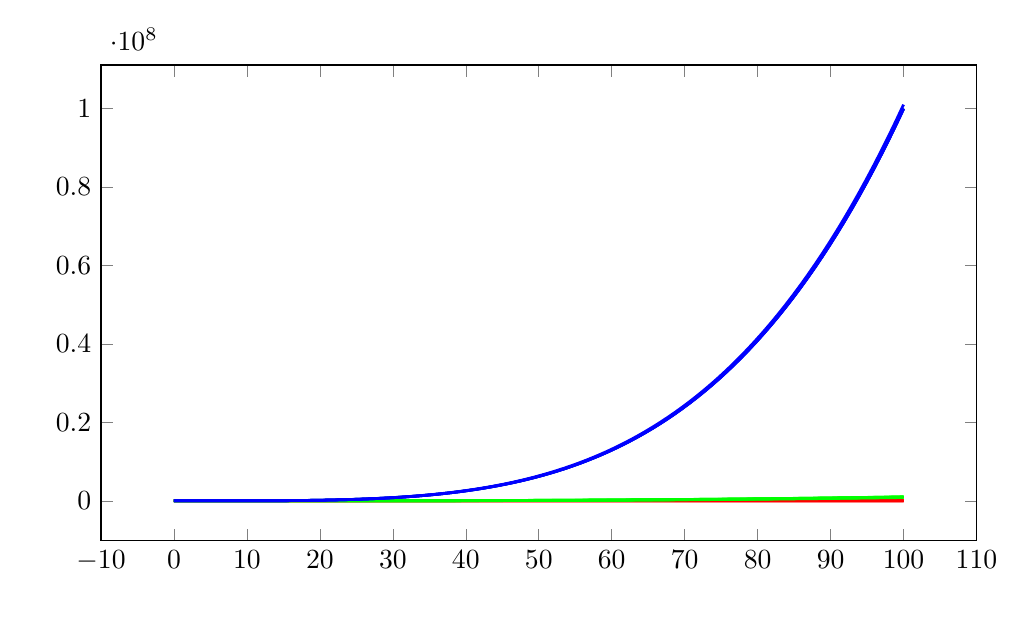
\begin{tikzpicture}[line width=1]
\begin{axis}[width=5in, height=3in,
             scatter/classes={a={mark=*,draw=black}},
             xlabel={\mbox{}},
             xlabel style={name=xlabel}, 
             ylabel={\mbox{}}, 
             legend style={
                at={(xlabel.south)},
                yshift=-1ex,
                anchor=north,
                legend cell align=left,
                },
        ]
]
\addplot[draw=red, line width=1] coordinates {(0.0,0.0)
(1.0101,1.0203)
(2.0202,4.0812)
(3.0303,9.1827)
(4.0404,16.3249)
(5.0505,25.5076)
(6.0606,36.7309)
(7.0707,49.9949)
(8.0808,65.2995)
(9.0909,82.6446)
(10.101,102.0304)
(11.1111,123.4568)
(12.1212,146.9238)
(13.1313,172.4314)
(14.1414,199.9796)
(15.1515,229.5684)
(16.1616,261.1978)
(17.1717,294.8679)
(18.1818,330.5785)
(19.1919,368.3298)
(20.202,408.1216)
(21.2121,449.9541)
(22.2222,493.8272)
(23.2323,539.7408)
(24.2424,587.6951)
(25.2525,637.69)
(26.2626,689.7255)
(27.2727,743.8017)
(28.2828,799.9184)
(29.2929,858.0757)
(30.303,918.2736)
(31.3131,980.5122)
(32.3232,1044.7913)
(33.3333,1111.1111)
(34.3434,1179.4715)
(35.3535,1249.8725)
(36.3636,1322.314)
(37.3737,1396.7962)
(38.3838,1473.319)
(39.3939,1551.8825)
(40.404,1632.4865)
(41.4141,1715.1311)
(42.4242,1799.8163)
(43.4343,1886.5422)
(44.4444,1975.3086)
(45.4545,2066.1157)
(46.4646,2158.9634)
(47.4747,2253.8516)
(48.4848,2350.7805)
(49.4949,2449.75)
(50.5051,2550.7601)
(51.5152,2653.8108)
(52.5253,2758.9022)
(53.5354,2866.0341)
(54.5455,2975.2066)
(55.5556,3086.4198)
(56.5657,3199.6735)
(57.5758,3314.9679)
(58.5859,3432.3028)
(59.596,3551.6784)
(60.6061,3673.0946)
(61.6162,3796.5514)
(62.6263,3922.0488)
(63.6364,4049.5868)
(64.6465,4179.1654)
(65.6566,4310.7846)
(66.6667,4444.4444)
(67.6768,4580.1449)
(68.6869,4717.8859)
(69.697,4857.6676)
(70.7071,4999.4898)
(71.7172,5143.3527)
(72.7273,5289.2562)
(73.7374,5437.2003)
(74.7475,5587.185)
(75.7576,5739.2103)
(76.7677,5893.2762)
(77.7778,6049.3827)
(78.7879,6207.5298)
(79.798,6367.7176)
(80.8081,6529.9459)
(81.8182,6694.2149)
(82.8283,6860.5244)
(83.8384,7028.8746)
(84.8485,7199.2654)
(85.8586,7371.6968)
(86.8687,7546.1688)
(87.8788,7722.6814)
(88.8889,7901.2346)
(89.899,8081.8284)
(90.9091,8264.4628)
(91.9192,8449.1378)
(92.9293,8635.8535)
(93.9394,8824.6097)
(94.9495,9015.4066)
(95.9596,9208.2441)
(96.9697,9403.1221)
(97.9798,9600.0408)
(98.9899,9799.0001)
(100.0,10000.0)};\addplot[draw=red, line width=1] coordinates {(0.0,2.0)
(1.0101,3.0203)
(2.0202,6.0812)
(3.0303,11.1827)
(4.0404,18.3249)
(5.0505,27.5076)
(6.0606,38.7309)
(7.0707,51.9949)
(8.0808,67.2995)
(9.0909,84.6446)
(10.101,104.0304)
(11.1111,125.4568)
(12.1212,148.9238)
(13.1313,174.4314)
(14.1414,201.9796)
(15.1515,231.5684)
(16.1616,263.1978)
(17.1717,296.8679)
(18.1818,332.5785)
(19.1919,370.3298)
(20.202,410.1216)
(21.2121,451.9541)
(22.2222,495.8272)
(23.2323,541.7408)
(24.2424,589.6951)
(25.2525,639.69)
(26.2626,691.7255)
(27.2727,745.8017)
(28.2828,801.9184)
(29.2929,860.0757)
(30.303,920.2736)
(31.3131,982.5122)
(32.3232,1046.7913)
(33.3333,1113.1111)
(34.3434,1181.4715)
(35.3535,1251.8725)
(36.3636,1324.314)
(37.3737,1398.7962)
(38.3838,1475.319)
(39.3939,1553.8825)
(40.404,1634.4865)
(41.4141,1717.1311)
(42.4242,1801.8163)
(43.4343,1888.5422)
(44.4444,1977.3086)
(45.4545,2068.1157)
(46.4646,2160.9634)
(47.4747,2255.8516)
(48.4848,2352.7805)
(49.4949,2451.75)
(50.5051,2552.7601)
(51.5152,2655.8108)
(52.5253,2760.9022)
(53.5354,2868.0341)
(54.5455,2977.2066)
(55.5556,3088.4198)
(56.5657,3201.6735)
(57.5758,3316.9679)
(58.5859,3434.3028)
(59.596,3553.6784)
(60.6061,3675.0946)
(61.6162,3798.5514)
(62.6263,3924.0488)
(63.6364,4051.5868)
(64.6465,4181.1654)
(65.6566,4312.7846)
(66.6667,4446.4444)
(67.6768,4582.1449)
(68.6869,4719.8859)
(69.697,4859.6676)
(70.7071,5001.4898)
(71.7172,5145.3527)
(72.7273,5291.2562)
(73.7374,5439.2003)
(74.7475,5589.185)
(75.7576,5741.2103)
(76.7677,5895.2762)
(77.7778,6051.3827)
(78.7879,6209.5298)
(79.798,6369.7176)
(80.8081,6531.9459)
(81.8182,6696.2149)
(82.8283,6862.5244)
(83.8384,7030.8746)
(84.8485,7201.2654)
(85.8586,7373.6968)
(86.8687,7548.1688)
(87.8788,7724.6814)
(88.8889,7903.2346)
(89.899,8083.8284)
(90.9091,8266.4628)
(91.9192,8451.1378)
(92.9293,8637.8535)
(93.9394,8826.6097)
(94.9495,9017.4066)
(95.9596,9210.2441)
(96.9697,9405.1221)
(97.9798,9602.0408)
(98.9899,9801.0001)
(100.0,10002.0)};\addplot[draw=red, line width=1] coordinates {(0.0,1.0)
(1.0101,2.0203)
(2.0202,5.0812)
(3.0303,10.1827)
(4.0404,17.3249)
(5.0505,26.5076)
(6.0606,37.7309)
(7.0707,50.9949)
(8.0808,66.2995)
(9.0909,83.6446)
(10.101,103.0304)
(11.1111,124.4568)
(12.1212,147.9238)
(13.1313,173.4314)
(14.1414,200.9796)
(15.1515,230.5684)
(16.1616,262.1978)
(17.1717,295.8679)
(18.1818,331.5785)
(19.1919,369.3298)
(20.202,409.1216)
(21.2121,450.9541)
(22.2222,494.8272)
(23.2323,540.7408)
(24.2424,588.6951)
(25.2525,638.69)
(26.2626,690.7255)
(27.2727,744.8017)
(28.2828,800.9184)
(29.2929,859.0757)
(30.303,919.2736)
(31.3131,981.5122)
(32.3232,1045.7913)
(33.3333,1112.1111)
(34.3434,1180.4715)
(35.3535,1250.8725)
(36.3636,1323.314)
(37.3737,1397.7962)
(38.3838,1474.319)
(39.3939,1552.8825)
(40.404,1633.4865)
(41.4141,1716.1311)
(42.4242,1800.8163)
(43.4343,1887.5422)
(44.4444,1976.3086)
(45.4545,2067.1157)
(46.4646,2159.9634)
(47.4747,2254.8516)
(48.4848,2351.7805)
(49.4949,2450.75)
(50.5051,2551.7601)
(51.5152,2654.8108)
(52.5253,2759.9022)
(53.5354,2867.0341)
(54.5455,2976.2066)
(55.5556,3087.4198)
(56.5657,3200.6735)
(57.5758,3315.9679)
(58.5859,3433.3028)
(59.596,3552.6784)
(60.6061,3674.0946)
(61.6162,3797.5514)
(62.6263,3923.0488)
(63.6364,4050.5868)
(64.6465,4180.1654)
(65.6566,4311.7846)
(66.6667,4445.4444)
(67.6768,4581.1449)
(68.6869,4718.8859)
(69.697,4858.6676)
(70.7071,5000.4898)
(71.7172,5144.3527)
(72.7273,5290.2562)
(73.7374,5438.2003)
(74.7475,5588.185)
(75.7576,5740.2103)
(76.7677,5894.2762)
(77.7778,6050.3827)
(78.7879,6208.5298)
(79.798,6368.7176)
(80.8081,6530.9459)
(81.8182,6695.2149)
(82.8283,6861.5244)
(83.8384,7029.8746)
(84.8485,7200.2654)
(85.8586,7372.6968)
(86.8687,7547.1688)
(87.8788,7723.6814)
(88.8889,7902.2346)
(89.899,8082.8284)
(90.9091,8265.4628)
(91.9192,8450.1378)
(92.9293,8636.8535)
(93.9394,8825.6097)
(94.9495,9016.4066)
(95.9596,9209.2441)
(96.9697,9404.1221)
(97.9798,9601.0408)
(98.9899,9800.0001)
(100.0,10001.0)};\addplot[draw=red, line width=1] coordinates {(0.0,-5.0)
(1.0101,1.0708)
(2.0202,9.1822)
(3.0303,19.3343)
(4.0404,31.5269)
(5.0505,45.7601)
(6.0606,62.034)
(7.0707,80.3484)
(8.0808,100.7035)
(9.0909,123.0992)
(10.101,147.5355)
(11.1111,174.0123)
(12.1212,202.5298)
(13.1313,233.088)
(14.1414,265.6867)
(15.1515,300.326)
(16.1616,337.0059)
(17.1717,375.7265)
(18.1818,416.4876)
(19.1919,459.2894)
(20.202,504.1317)
(21.2121,551.0147)
(22.2222,599.9383)
(23.2323,650.9025)
(24.2424,703.9073)
(25.2525,758.9527)
(26.2626,816.0387)
(27.2727,875.1653)
(28.2828,936.3325)
(29.2929,999.5404)
(30.303,1064.7888)
(31.3131,1132.0778)
(32.3232,1201.4075)
(33.3333,1272.7778)
(34.3434,1346.1887)
(35.3535,1421.6401)
(36.3636,1499.1322)
(37.3737,1578.6649)
(38.3838,1660.2382)
(39.3939,1743.8522)
(40.404,1829.5067)
(41.4141,1917.2018)
(42.4242,2006.9376)
(43.4343,2098.7139)
(44.4444,2192.5309)
(45.4545,2288.3884)
(46.4646,2386.2866)
(47.4747,2486.2254)
(48.4848,2588.2048)
(49.4949,2692.2248)
(50.5051,2798.2854)
(51.5152,2906.3866)
(52.5253,3016.5284)
(53.5354,3128.7108)
(54.5455,3242.9339)
(55.5556,3359.1975)
(56.5657,3477.5018)
(57.5758,3597.8466)
(58.5859,3720.2321)
(59.596,3844.6582)
(60.6061,3971.1249)
(61.6162,4099.6322)
(62.6263,4230.1801)
(63.6364,4362.7686)
(64.6465,4497.3977)
(65.6566,4634.0674)
(66.6667,4772.7778)
(67.6768,4913.5287)
(68.6869,5056.3203)
(69.697,5201.1524)
(70.7071,5348.0252)
(71.7172,5496.9386)
(72.7273,5647.8926)
(73.7374,5800.8872)
(74.7475,5955.9224)
(75.7576,6112.9982)
(76.7677,6272.1146)
(77.7778,6433.2716)
(78.7879,6596.4692)
(79.798,6761.7075)
(80.8081,6928.9863)
(81.8182,7098.3058)
(82.8283,7269.6659)
(83.8384,7443.0665)
(84.8485,7618.5078)
(85.8586,7795.9897)
(86.8687,7975.5122)
(87.8788,8157.0753)
(88.8889,8340.679)
(89.899,8526.3233)
(90.9091,8714.0083)
(91.9192,8903.7338)
(92.9293,9095.4999)
(93.9394,9289.3067)
(94.9495,9485.1541)
(95.9596,9683.042)
(96.9697,9882.9706)
(97.9798,10084.9398)
(98.9899,10288.9496)
(100.0,10495.0)};\addplot[draw=red, line width=1] coordinates {(0.0,-8.0)
(1.0101,-10.01)
(2.0202,-9.9794)
(3.0303,-7.9082)
(4.0404,-3.7963)
(5.0505,2.3561)
(6.0606,10.5491)
(7.0707,20.7828)
(8.0808,33.057)
(9.0909,47.3719)
(10.101,63.7274)
(11.1111,82.1235)
(12.1212,102.5601)
(13.1313,125.0374)
(14.1414,149.5554)
(15.1515,176.1139)
(16.1616,204.713)
(17.1717,235.3527)
(18.1818,268.0331)
(19.1919,302.754)
(20.202,339.5156)
(21.2121,378.3177)
(22.2222,419.1605)
(23.2323,462.0439)
(24.2424,506.9679)
(25.2525,553.9325)
(26.2626,602.9377)
(27.2727,653.9835)
(28.2828,707.0699)
(29.2929,762.1969)
(30.303,819.3646)
(31.3131,878.5728)
(32.3232,939.8217)
(33.3333,1003.1111)
(34.3434,1068.4412)
(35.3535,1135.8119)
(36.3636,1205.2231)
(37.3737,1276.675)
(38.3838,1350.1675)
(39.3939,1425.7006)
(40.404,1503.2744)
(41.4141,1582.8887)
(42.4242,1664.5436)
(43.4343,1748.2392)
(44.4444,1833.9753)
(45.4545,1921.7521)
(46.4646,2011.5694)
(47.4747,2103.4274)
(48.4848,2197.326)
(49.4949,2293.2652)
(50.5051,2391.245)
(51.5152,2491.2654)
(52.5253,2593.3264)
(53.5354,2697.428)
(54.5455,2803.5702)
(55.5556,2911.7531)
(56.5657,3021.9765)
(57.5758,3134.2406)
(58.5859,3248.5453)
(59.596,3364.8905)
(60.6061,3483.2764)
(61.6162,3603.7029)
(62.6263,3726.17)
(63.6364,3850.6777)
(64.6465,3977.226)
(65.6566,4105.8149)
(66.6667,4236.4444)
(67.6768,4369.1146)
(68.6869,4503.8253)
(69.697,4640.5767)
(70.7071,4779.3686)
(71.7172,4920.2012)
(72.7273,5063.0744)
(73.7374,5207.9882)
(74.7475,5354.9426)
(75.7576,5503.9376)
(76.7677,5654.9732)
(77.7778,5808.0494)
(78.7879,5963.1662)
(79.798,6120.3236)
(80.8081,6279.5217)
(81.8182,6440.7603)
(82.8283,6604.0396)
(83.8384,6769.3595)
(84.8485,6936.7199)
(85.8586,7106.121)
(86.8687,7277.5627)
(87.8788,7451.045)
(88.8889,7626.5679)
(89.899,7804.1314)
(90.9091,7983.7355)
(91.9192,8165.3803)
(92.9293,8349.0656)
(93.9394,8534.7916)
(94.9495,8722.5581)
(95.9596,8912.3653)
(96.9697,9104.213)
(97.9798,9298.1014)
(98.9899,9494.0304)
(100.0,9692.0)};\addplot[draw=green, line width=1] coordinates {(0.0,0.0)
(1.0101,1.0306)
(2.0202,8.2449)
(3.0303,27.8265)
(4.0404,65.959)
(5.0505,128.8263)
(6.0606,222.6118)
(7.0707,353.4993)
(8.0808,527.6724)
(9.0909,751.3148)
(10.101,1030.6102)
(11.1111,1371.7421)
(12.1212,1780.8943)
(13.1313,2264.2505)
(14.1414,2827.9943)
(15.1515,3478.3093)
(16.1616,4221.3792)
(17.1717,5063.3877)
(18.1818,6010.5184)
(19.1919,7068.955)
(20.202,8244.8812)
(21.2121,9544.4806)
(22.2222,10973.9369)
(23.2323,12539.4337)
(24.2424,14247.1547)
(25.2525,16103.2836)
(26.2626,18114.004)
(27.2727,20285.4996)
(28.2828,22623.9541)
(29.2929,25135.551)
(30.303,27826.4741)
(31.3131,30702.907)
(32.3232,33771.0335)
(33.3333,37037.037)
(34.3434,40507.1014)
(35.3535,44187.4103)
(36.3636,48084.1473)
(37.3737,52203.496)
(38.3838,56551.6403)
(39.3939,61134.7636)
(40.404,65959.0497)
(41.4141,71030.6823)
(42.4242,76355.845)
(43.4343,81940.7214)
(44.4444,87791.4952)
(45.4545,93914.3501)
(46.4646,100315.4698)
(47.4747,107001.0378)
(48.4848,113977.2379)
(49.4949,121250.2538)
(50.5051,128826.269)
(51.5152,136711.4673)
(52.5253,144912.0323)
(53.5354,153434.1476)
(54.5455,162283.997)
(55.5556,171467.7641)
(56.5657,180991.6325)
(57.5758,190861.7859)
(58.5859,201084.408)
(59.596,211665.6824)
(60.6061,222611.7929)
(61.6162,233928.9229)
(62.6263,245623.2563)
(63.6364,257700.9767)
(64.6465,270168.2677)
(65.6566,283031.313)
(66.6667,296296.2963)
(67.6768,309969.4012)
(68.6869,324056.8114)
(69.697,338564.7105)
(70.7071,353499.2822)
(71.7172,368866.7102)
(72.7273,384673.1781)
(73.7374,400924.8696)
(74.7475,417627.9683)
(75.7576,434788.6579)
(76.7677,452413.1221)
(77.7778,470507.5446)
(78.7879,489078.1089)
(79.798,508130.9988)
(80.8081,527672.3979)
(81.8182,547708.4899)
(82.8283,568245.4584)
(83.8384,589289.4871)
(84.8485,610846.7596)
(85.8586,632923.4597)
(86.8687,655525.7709)
(87.8788,678659.877)
(88.8889,702331.9616)
(89.899,726548.2083)
(90.9091,751314.8009)
(91.9192,776637.9229)
(92.9293,802523.7581)
(93.9394,828978.4901)
(94.9495,856008.3026)
(95.9596,883619.3792)
(96.9697,911817.9036)
(97.9798,940610.0594)
(98.9899,970002.0303)
(100.0,1000000.0)};\addplot[draw=green, line width=1] coordinates {(0.0,-5.0)
(1.0101,-21.1105)
(2.0202,-24.9155)
(3.0303,-10.2314)
(4.0404,29.1256)
(5.0505,99.339)
(6.0606,206.5925)
(7.0707,357.0698)
(8.0808,556.9546)
(9.0909,812.4305)
(10.101,1129.6812)
(11.1111,1514.8903)
(12.1212,1974.2415)
(13.1313,2513.9184)
(14.1414,3140.1048)
(15.1515,3858.9842)
(16.1616,4676.7404)
(17.1717,5599.5569)
(18.1818,6633.6176)
(19.1919,7785.1059)
(20.202,9060.2057)
(21.2121,10465.1005)
(22.2222,12005.9739)
(23.2323,13689.0098)
(24.2424,15520.3917)
(25.2525,17506.3032)
(26.2626,19652.9281)
(27.2727,21966.45)
(28.2828,24453.0526)
(29.2929,27118.9195)
(30.303,29970.2344)
(31.3131,33013.181)
(32.3232,36253.9429)
(33.3333,39698.7037)
(34.3434,43353.6472)
(35.3535,47224.957)
(36.3636,51318.8167)
(37.3737,55641.41)
(38.3838,60198.9206)
(39.3939,64997.5322)
(40.404,70043.4284)
(41.4141,75342.7928)
(42.4242,80901.8091)
(43.4343,86726.6611)
(44.4444,92823.5322)
(45.4545,99198.6063)
(46.4646,105858.067)
(47.4747,112808.0978)
(48.4848,120054.8826)
(49.4949,127604.6049)
(50.5051,135463.4484)
(51.5152,143637.5968)
(52.5253,152133.2337)
(53.5354,160956.5428)
(54.5455,170113.7077)
(55.5556,179610.9122)
(56.5657,189454.3399)
(57.5758,199650.1743)
(58.5859,210204.5993)
(59.596,221123.7984)
(60.6061,232413.9554)
(61.6162,244081.2538)
(62.6263,256131.8774)
(63.6364,268572.0098)
(64.6465,281407.8346)
(65.6566,294645.5356)
(66.6667,308291.2963)
(67.6768,322351.3005)
(68.6869,336831.7318)
(69.697,351738.7738)
(70.7071,367078.6103)
(71.7172,382857.4249)
(72.7273,399081.4012)
(73.7374,415756.7229)
(74.7475,432889.5737)
(75.7576,450486.1373)
(76.7677,468552.5972)
(77.7778,487095.1372)
(78.7879,506119.9409)
(79.798,525633.1919)
(80.8081,545641.074)
(81.8182,566149.7708)
(82.8283,587165.466)
(83.8384,608694.3432)
(84.8485,630742.5861)
(85.8586,653316.3783)
(86.8687,676421.9035)
(87.8788,700065.3453)
(88.8889,724252.8875)
(89.899,748990.7137)
(90.9091,774285.0075)
(91.9192,800141.9526)
(92.9293,826567.7327)
(93.9394,853568.5315)
(94.9495,881150.5325)
(95.9596,909319.9194)
(96.9697,938082.876)
(97.9798,967445.5859)
(98.9899,997414.2326)
(100.0,1027995.0)};\addplot[draw=green, line width=1] coordinates {(0.0,-15.0)
(1.0101,-38.2016)
(2.0202,-53.179)
(3.0303,-53.7484)
(4.0404,-33.7262)
(5.0505,13.0712)
(6.0606,92.8276)
(7.0707,211.7265)
(8.0808,375.9517)
(9.0909,591.6867)
(10.101,865.1153)
(11.1111,1202.4211)
(12.1212,1609.7878)
(13.1313,2093.3991)
(14.1414,2659.4385)
(15.1515,3314.0898)
(16.1616,4063.5366)
(17.1717,4913.9626)
(18.1818,5871.5515)
(19.1919,6942.4868)
(20.202,8132.9523)
(21.2121,9449.1317)
(22.2222,10897.2085)
(23.2323,12483.3665)
(24.2424,14213.7893)
(25.2525,16094.6605)
(26.2626,18132.1639)
(27.2727,20332.4831)
(28.2828,22701.8017)
(29.2929,25246.3035)
(30.303,27972.172)
(31.3131,30885.591)
(32.3232,33992.744)
(33.3333,37299.8148)
(34.3434,40812.987)
(35.3535,44538.4444)
(36.3636,48482.3704)
(37.3737,52650.9488)
(38.3838,57050.3634)
(39.3939,61686.7976)
(40.404,66566.4352)
(41.4141,71695.4599)
(42.4242,77080.0552)
(43.4343,82726.405)
(44.4444,88640.6927)
(45.4545,94829.1022)
(46.4646,101297.817)
(47.4747,108053.0208)
(48.4848,115100.8973)
(49.4949,122447.6301)
(50.5051,130099.4029)
(51.5152,138062.3993)
(52.5253,146342.8031)
(53.5354,154946.7979)
(54.5455,163880.5672)
(55.5556,173150.2949)
(56.5657,182762.1646)
(57.5758,192722.3598)
(58.5859,203037.0644)
(59.596,213712.4618)
(60.6061,224754.7359)
(61.6162,236170.0703)
(62.6263,247964.6485)
(63.6364,260144.6544)
(64.6465,272716.2715)
(65.6566,285685.6835)
(66.6667,299059.0741)
(67.6768,312842.6269)
(68.6869,327042.5256)
(69.697,341664.9538)
(70.7071,356716.0953)
(71.7172,372202.1336)
(72.7273,388129.2524)
(73.7374,404503.6355)
(74.7475,421331.4664)
(75.7576,438618.9288)
(76.7677,456372.2064)
(77.7778,474597.4829)
(78.7879,493300.9418)
(79.798,512488.7669)
(80.8081,532167.1418)
(81.8182,552342.2502)
(82.8283,573020.2757)
(83.8384,594207.4021)
(84.8485,615909.8129)
(85.8586,638133.6918)
(86.8687,660885.2225)
(87.8788,684170.5887)
(88.8889,707995.9739)
(89.899,732367.562)
(90.9091,757291.5364)
(91.9192,782774.081)
(92.9293,808821.3793)
(93.9394,835439.615)
(94.9495,862634.9718)
(95.9596,890413.6333)
(96.9697,918781.7833)
(97.9798,947745.6052)
(98.9899,977311.2829)
(100.0,1007485.0)};\addplot[draw=green, line width=1] coordinates {(0.0,1.0)
(1.0101,-18.3245)
(2.0202,-62.0744)
(3.0303,-124.0661)
(4.0404,-198.1159)
(5.0505,-278.0403)
(6.0606,-357.6554)
(7.0707,-430.7777)
(8.0808,-491.2235)
(9.0909,-532.8092)
(10.101,-549.351)
(11.1111,-534.6653)
(12.1212,-482.5685)
(13.1313,-386.8768)
(14.1414,-241.4067)
(15.1515,-39.9745)
(16.1616,223.6035)
(17.1717,555.511)
(18.1818,961.9316)
(19.1919,1449.049)
(20.202,2023.0468)
(21.2121,2690.1087)
(22.2222,3456.4184)
(23.2323,4328.1595)
(24.2424,5311.5156)
(25.2525,6412.6705)
(26.2626,7637.8078)
(27.2727,8993.1112)
(28.2828,10484.7643)
(29.2929,12118.9508)
(30.303,13901.8543)
(31.3131,15839.6585)
(32.3232,17938.5471)
(33.3333,20204.7037)
(34.3434,22644.312)
(35.3535,25263.5557)
(36.3636,28068.6183)
(37.3737,31065.6837)
(38.3838,34260.9353)
(39.3939,37660.557)
(40.404,41270.7323)
(41.4141,45097.645)
(42.4242,49147.4786)
(43.4343,53426.4168)
(44.4444,57940.6433)
(45.4545,62696.3418)
(46.4646,67699.696)
(47.4747,72956.8894)
(48.4848,78474.1057)
(49.4949,84257.5287)
(50.5051,90313.3419)
(51.5152,96647.729)
(52.5253,103266.8737)
(53.5354,110176.9597)
(54.5455,117384.1705)
(55.5556,124894.69)
(56.5657,132714.7017)
(57.5758,140850.3892)
(58.5859,149307.9363)
(59.596,158093.5266)
(60.6061,167213.3438)
(61.6162,176673.5715)
(62.6263,186480.3935)
(63.6364,196639.9932)
(64.6465,207158.5545)
(65.6566,218042.261)
(66.6667,229297.2963)
(67.6768,240929.8441)
(68.6869,252946.0881)
(69.697,265352.2118)
(70.7071,278154.3991)
(71.7172,291358.8335)
(72.7273,304971.6987)
(73.7374,318999.1784)
(74.7475,333447.4562)
(75.7576,348322.7158)
(76.7677,363631.1408)
(77.7778,379378.915)
(78.7879,395572.2219)
(79.798,412217.2452)
(80.8081,429320.1686)
(81.8182,446887.1758)
(82.8283,464924.4504)
(83.8384,483438.1761)
(84.8485,502434.5365)
(85.8586,521919.7153)
(86.8687,541899.8961)
(87.8788,562381.2627)
(88.8889,583369.9986)
(89.899,604872.2876)
(90.9091,626894.3133)
(91.9192,649442.2593)
(92.9293,672522.3094)
(93.9394,696140.6472)
(94.9495,720303.4563)
(95.9596,745016.9204)
(96.9697,770287.2231)
(97.9798,796120.5482)
(98.9899,822523.0793)
(100.0,849501.0)};\addplot[draw=green, line width=1] coordinates {(0.0,-100.0)
(1.0101,-101.061)
(2.0202,-110.2226)
(3.0303,-121.3012)
(4.0404,-128.113)
(5.0505,-124.4744)
(6.0606,-104.2018)
(7.0707,-61.1115)
(8.0808,10.9802)
(9.0909,118.2569)
(10.101,266.9024)
(11.1111,463.1001)
(12.1212,713.0339)
(13.1313,1022.8874)
(14.1414,1398.8442)
(15.1515,1847.088)
(16.1616,2373.8024)
(17.1717,2985.1712)
(18.1818,3687.3779)
(19.1919,4486.6063)
(20.202,5389.04)
(21.2121,6400.8626)
(22.2222,7528.2579)
(23.2323,8777.4094)
(24.2424,10154.5009)
(25.2525,11665.716)
(26.2626,13317.2384)
(27.2727,15115.2517)
(28.2828,17065.9396)
(29.2929,19175.4857)
(30.303,21450.0737)
(31.3131,23895.8874)
(32.3232,26519.1102)
(33.3333,29325.9259)
(34.3434,32322.5182)
(35.3535,35515.0707)
(36.3636,38909.7671)
(37.3737,42512.791)
(38.3838,46330.3261)
(39.3939,50368.5561)
(40.404,54633.6646)
(41.4141,59131.8352)
(42.4242,63869.2517)
(43.4343,68852.0978)
(44.4444,74086.5569)
(45.4545,79578.8129)
(46.4646,85335.0494)
(47.4747,91361.45)
(48.4848,97664.1985)
(49.4949,104249.4784)
(50.5051,111123.4734)
(51.5152,118292.3672)
(52.5253,125762.3435)
(53.5354,133539.5858)
(54.5455,141630.278)
(55.5556,150040.6036)
(56.5657,158776.7462)
(57.5758,167844.8897)
(58.5859,177251.2175)
(59.596,187001.9134)
(60.6061,197103.1611)
(61.6162,207561.1441)
(62.6263,218382.0463)
(63.6364,229572.0511)
(64.6465,241137.3423)
(65.6566,253084.1036)
(66.6667,265418.5185)
(67.6768,278146.7708)
(68.6869,291275.0442)
(69.697,304809.5222)
(70.7071,318756.3886)
(71.7172,333121.827)
(72.7273,347912.021)
(73.7374,363133.1544)
(74.7475,378791.4108)
(75.7576,394892.9738)
(76.7677,411444.0272)
(77.7778,428450.7545)
(78.7879,445919.3394)
(79.798,463855.9656)
(80.8081,482266.8168)
(81.8182,501158.0766)
(82.8283,520535.9287)
(83.8384,540406.5567)
(84.8485,560776.1444)
(85.8586,581650.8752)
(86.8687,603036.933)
(87.8788,624940.5014)
(88.8889,647367.7641)
(89.899,670324.9046)
(90.9091,693818.1067)
(91.9192,717853.554)
(92.9293,742437.4302)
(93.9394,767575.919)
(94.9495,793275.2039)
(95.9596,819541.4688)
(96.9697,846380.8971)
(97.9798,873799.6727)
(98.9899,901803.9791)
(100.0,930400.0)};\addplot[draw=green, line width=1] coordinates {(0.0,0.0)
(1.0101,1.041)
(2.0202,16.6563)
(3.0303,84.3226)
(4.0404,266.5012)
(5.0505,650.6377)
(6.0606,1349.1624)
(7.0707,2499.4899)
(8.0808,4264.0194)
(9.0909,6830.1346)
(10.101,10410.2036)
(11.1111,15241.579)
(12.1212,21586.5981)
(13.1313,29732.5824)
(14.1414,39991.838)
(15.1515,52701.6555)
(16.1616,68224.31)
(17.1717,86947.0611)
(18.1818,109282.1529)
(19.1919,135666.8138)
(20.202,166563.2569)
(21.2121,202458.6798)
(22.2222,243865.2644)
(23.2323,291320.1774)
(24.2424,345385.5695)
(25.2525,406648.5764)
(26.2626,475721.3181)
(27.2727,553240.8988)
(28.2828,639869.4077)
(29.2929,736293.9182)
(30.303,843226.4881)
(31.3131,961404.1599)
(32.3232,1091588.9605)
(33.3333,1234567.9012)
(34.3434,1391152.978)
(35.3535,1562181.1713)
(36.3636,1748514.4457)
(37.3737,1951039.7508)
(38.3838,2170669.0204)
(39.3939,2408339.1727)
(40.404,2665012.1106)
(41.4141,2941674.7213)
(42.4242,3239338.8767)
(43.4343,3559041.433)
(44.4444,3901844.2311)
(45.4545,4268834.096)
(46.4646,4661122.8377)
(47.4747,5079847.2503)
(48.4848,5526169.1124)
(49.4949,6001275.1875)
(50.5051,6506377.223)
(51.5152,7042711.9513)
(52.5253,7611541.089)
(53.5354,8214151.3371)
(54.5455,8851854.3815)
(55.5556,9525986.8922)
(56.5657,10237910.5239)
(57.5758,10989011.9156)
(58.5859,11780702.691)
(59.596,12614419.4582)
(60.6061,13491623.8097)
(61.6162,14413802.3226)
(62.6263,15382466.5584)
(63.6364,16399153.0633)
(64.6465,17465423.3677)
(65.6566,18582863.9867)
(66.6667,19753086.4198)
(67.6768,20977727.1509)
(68.6869,22258447.6486)
(69.697,23596934.3658)
(70.7071,24994898.74)
(71.7172,26454077.1932)
(72.7273,27976231.1318)
(73.7374,29563146.9467)
(74.7475,31216636.0133)
(75.7576,32938534.6916)
(76.7677,34730704.326)
(77.7778,36595031.2452)
(78.7879,38533426.7628)
(79.798,40547827.1766)
(80.8081,42640193.7689)
(81.8182,44812512.8065)
(82.8283,47066795.5408)
(83.8384,49405078.2076)
(84.8485,51829422.0273)
(85.8586,54341913.2045)
(86.8687,56944662.9286)
(87.8788,59639807.3733)
(88.8889,62429507.697)
(89.899,65315950.0423)
(90.9091,68301345.5365)
(91.9192,71387930.2913)
(92.9293,74577965.403)
(93.9394,77873736.9521)
(94.9495,81277556.004)
(95.9596,84791758.6083)
(96.9697,88418705.7991)
(97.9798,92160783.5952)
(98.9899,96020402.9996)
(100.0,100000000.0)};\addplot[draw=blue, line width=1] coordinates {(0.0,-9.0)
(1.0101,-27.1407)
(2.0202,-28.6665)
(3.0303,23.8993)
(4.0404,193.018)
(5.0505,566.1352)
(6.0606,1255.6812)
(7.0707,2399.0706)
(8.0808,4158.7027)
(9.0909,6721.961)
(10.101,10301.2138)
(11.1111,15133.8136)
(12.1212,21482.0976)
(13.1313,29633.3875)
(14.1414,39899.9893)
(15.1515,52619.1936)
(16.1616,68153.2755)
(17.1717,86889.4947)
(18.1818,109240.095)
(19.1919,135642.3052)
(20.202,166558.3381)
(21.2121,202475.3915)
(22.2222,243905.6472)
(23.2323,291386.2717)
(24.2424,345479.4162)
(25.2525,406772.216)
(26.2626,475876.7911)
(27.2727,553430.246)
(28.2828,640094.6696)
(29.2929,736557.1353)
(30.303,843529.7011)
(31.3131,961749.4095)
(32.3232,1091978.2872)
(33.3333,1235003.3457)
(34.3434,1391636.5808)
(35.3535,1562714.973)
(36.3636,1749100.4871)
(37.3737,1951680.0723)
(38.3838,2171365.6627)
(39.3939,2409094.1763)
(40.404,2665827.5162)
(41.4141,2942552.5696)
(42.4242,3240281.2082)
(43.4343,3560050.2884)
(44.4444,3902921.6508)
(45.4545,4269982.1208)
(46.4646,4662343.5081)
(47.4747,5081142.6069)
(48.4848,5527541.196)
(49.4949,6002726.0385)
(50.5051,6507908.8821)
(51.5152,7044326.4591)
(52.5253,7613240.4861)
(53.5354,8215937.6642)
(54.5455,8853729.6791)
(55.5556,9527953.2009)
(56.5657,10239969.8843)
(57.5758,10991166.3683)
(58.5859,11782954.2767)
(59.596,12616770.2174)
(60.6061,13494075.7831)
(61.6162,14416357.5507)
(62.6263,15385127.082)
(63.6364,16401920.9228)
(64.6465,17468300.6038)
(65.6566,18585852.64)
(66.6667,19756188.5309)
(67.6768,20980944.7604)
(68.6869,22261782.7971)
(69.697,23600389.094)
(70.7071,24998475.0884)
(71.7172,26457777.2025)
(72.7273,27980056.8425)
(73.7374,29567100.3995)
(74.7475,31220719.2488)
(75.7576,32942749.7504)
(76.7677,34735053.2486)
(77.7778,36599516.0724)
(78.7879,38538049.5351)
(79.798,40552589.9346)
(80.8081,42645098.5532)
(81.8182,44817561.6577)
(82.8283,47071990.4996)
(83.8384,49410421.3146)
(84.8485,51834915.323)
(85.8586,54347558.7295)
(86.8687,56950462.7236)
(87.8788,59645763.4789)
(88.8889,62435622.1538)
(89.899,65322224.8909)
(90.9091,68307782.8175)
(91.9192,71394532.0453)
(92.9293,74584733.6706)
(93.9394,77880673.774)
(94.9495,81284663.4207)
(95.9596,84799038.6604)
(96.9697,88426160.5273)
(97.9798,92168415.04)
(98.9899,96028213.2017)
(100.0,100007991.0)};\addplot[draw=blue, line width=1] coordinates {(0.0,-1.0)
(1.0101,-24.1809)
(2.0202,-26.6038)
(3.0303,35.3915)
(4.0404,230.4502)
(5.0505,652.2014)
(6.0606,1419.259)
(7.0707,2675.2215)
(8.0808,4588.6716)
(9.0909,7353.1766)
(10.101,11187.2885)
(11.1111,16334.5434)
(12.1212,23063.4621)
(13.1313,31667.5501)
(14.1414,42465.2969)
(15.1515,55800.1769)
(16.1616,72040.6488)
(17.1717,91580.1559)
(18.1818,114837.1258)
(19.1919,142254.9708)
(20.202,174302.0876)
(21.2121,211471.8574)
(22.2222,254282.6458)
(23.2323,303277.803)
(24.2424,359025.6637)
(25.2525,422119.5469)
(26.2626,493177.7564)
(27.2727,572843.5803)
(28.2828,661785.2911)
(29.2929,760696.146)
(30.303,870294.3865)
(31.3131,991323.2387)
(32.3232,1124550.9131)
(33.3333,1270770.6049)
(34.3434,1430800.4936)
(35.3535,1605483.7431)
(36.3636,1795688.5021)
(37.3737,2002307.9034)
(38.3838,2226260.0647)
(39.3939,2468488.0878)
(40.404,2729960.0593)
(41.4141,3011669.0501)
(42.4242,3314633.1156)
(43.4343,3639895.2958)
(44.4444,3988523.6152)
(45.4545,4361611.0825)
(46.4646,4760275.6913)
(47.4747,5185660.4194)
(48.4848,5638933.2292)
(49.4949,6121287.0675)
(50.5051,6633939.8658)
(51.5152,7178134.5398)
(52.5253,7755138.9899)
(53.5354,8366246.1009)
(54.5455,9012773.7422)
(55.5556,9696064.7674)
(56.5657,10417487.015)
(57.5758,11178433.3076)
(58.5859,11980321.4526)
(59.596,12824594.2416)
(60.6061,13712719.451)
(61.6162,14646189.8415)
(62.6263,15626523.1582)
(63.6364,16655262.1309)
(64.6465,17733974.4738)
(65.6566,18864252.8856)
(66.6667,20047715.0494)
(67.6768,21286003.6329)
(68.6869,22580786.2882)
(69.697,23933755.652)
(70.7071,25346629.3454)
(71.7172,26821149.974)
(72.7273,28359085.128)
(73.7374,29962227.3819)
(74.7475,31632394.2947)
(75.7576,33371428.4101)
(76.7677,35181197.2562)
(77.7778,37063593.3454)
(78.7879,39020534.1748)
(79.798,41053962.2259)
(80.8081,43165844.9647)
(81.8182,45358174.8418)
(82.8283,47632969.2921)
(83.8384,49992270.7351)
(84.8485,52438146.5748)
(85.8586,54972689.1995)
(86.8687,57598015.9823)
(87.8788,60316269.2807)
(88.8889,63129616.4364)
(89.899,66040249.7759)
(90.9091,69050386.6101)
(91.9192,72162269.2345)
(92.9293,75378164.9288)
(93.9394,78700365.9574)
(94.9495,82131189.5692)
(95.9596,85672977.9976)
(96.9697,89328098.4603)
(97.9798,93098943.1596)
(98.9899,96987929.2824)
(100.0,100997499.0)};\addplot[draw=blue, line width=1] coordinates {(0.0,1.0)
(1.0101,-18.314)
(2.0202,-53.6629)
(3.0303,-67.5699)
(4.0404,2.4262)
(5.0505,243.7712)
(6.0606,768.8952)
(7.0707,1715.2129)
(8.0808,3245.1234)
(9.0909,5546.0106)
(10.101,8830.2424)
(11.1111,13335.1716)
(12.1212,19323.1353)
(13.1313,27081.455)
(14.1414,36922.437)
(15.1515,49183.3718)
(16.1616,64226.5344)
(17.1717,82439.1845)
(18.1818,104233.5661)
(19.1919,130046.9077)
(20.202,160341.4225)
(21.2121,195604.3079)
(22.2222,236347.7459)
(23.2323,283108.9031)
(24.2424,336449.9304)
(25.2525,396957.9633)
(26.2626,465245.1219)
(27.2727,541948.5104)
(28.2828,627730.218)
(29.2929,723277.3179)
(30.303,829301.8683)
(31.3131,946540.9114)
(32.3232,1075756.4741)
(33.3333,1217735.5679)
(34.3434,1373290.1886)
(35.3535,1543257.3166)
(36.3636,1728498.9168)
(37.3737,1929901.9385)
(38.3838,2148378.3154)
(39.3939,2384864.9661)
(40.404,2640323.7931)
(41.4141,2915741.684)
(42.4242,3212130.5103)
(43.4343,3530527.1285)
(44.4444,3871993.3792)
(45.4545,4237616.0878)
(46.4646,4628507.0639)
(47.4747,5045803.1018)
(48.4848,5490665.9802)
(49.4949,5964282.4623)
(50.5051,6467864.2959)
(51.5152,7002648.213)
(52.5253,7569895.9304)
(53.5354,8170894.1492)
(54.5455,8806954.5551)
(55.5556,9479413.8182)
(56.5657,10189633.5931)
(57.5758,10939000.5189)
(58.5859,11728926.2193)
(59.596,12560847.3024)
(60.6061,13436225.3606)
(61.6162,14356546.9712)
(62.6263,15323323.6956)
(63.6364,16338092.0798)
(64.6465,17402413.6545)
(65.6566,18517874.9347)
(66.6667,19686087.4198)
(67.6768,20908687.5938)
(68.6869,22187336.9253)
(69.697,23523721.8672)
(70.7071,24919553.8569)
(71.7172,26376569.3165)
(72.7273,27896529.6524)
(73.7374,29481221.2555)
(74.7475,31132455.5012)
(75.7576,32852068.7495)
(76.7677,34641922.3446)
(77.7778,36503902.6156)
(78.7879,38439920.8758)
(79.798,40451913.423)
(80.8081,42541841.5396)
(81.8182,44711691.4925)
(82.8283,46963474.5329)
(83.8384,49299226.8967)
(84.8485,51721009.8041)
(85.8586,54230909.4601)
(86.8687,56831037.0538)
(87.8788,59523528.759)
(88.8889,62310545.734)
(89.899,65194274.1216)
(90.9091,68176925.0489)
(91.9192,71260734.6277)
(92.9293,74447963.9542)
(93.9394,77740899.1091)
(94.9495,81141851.1577)
(95.9596,84653156.1495)
(96.9697,88277175.1187)
(97.9798,92016294.084)
(98.9899,95872924.0486)
(100.0,99849501.0)};\addplot[draw=blue, line width=1] coordinates {(0.0,-100.0)
(1.0101,-108.0703)
(2.0202,-105.6475)
(3.0303,-55.2549)
(4.0404,105.5687)
(5.0505,464.269)
(6.0606,1133.2762)
(7.0707,2250.0051)
(8.0808,3976.8548)
(9.0909,6501.2089)
(10.101,10035.4357)
(11.1111,14816.8877)
(12.1212,21107.902)
(13.1313,29195.8004)
(14.1414,39392.8889)
(15.1515,52036.4581)
(16.1616,67488.783)
(17.1717,86137.1234)
(18.1818,108393.7231)
(19.1919,134695.8108)
(20.202,165505.5995)
(21.2121,201310.2868)
(22.2222,242622.0546)
(23.2323,289978.0694)
(24.2424,343940.4823)
(25.2525,405096.4287)
(26.2626,474058.0286)
(27.2727,551462.3864)
(28.2828,637971.5912)
(29.2929,734272.7163)
(30.303,841077.8196)
(31.3131,959123.9436)
(32.3232,1089173.1152)
(33.3333,1232012.3457)
(34.3434,1388453.631)
(35.3535,1559333.9516)
(36.3636,1745515.2722)
(37.3737,1947884.5422)
(38.3838,2167353.6954)
(39.3939,2404859.6502)
(40.404,2661364.3093)
(41.4141,2937854.5601)
(42.4242,3235342.2743)
(43.4343,3554864.3083)
(44.4444,3897482.5027)
(45.4545,4264283.6828)
(46.4646,4656379.6584)
(47.4747,5074907.2237)
(48.4848,5521028.1574)
(49.4949,5995929.2228)
(50.5051,6500822.1674)
(51.5152,7036943.7236)
(52.5253,7605555.6079)
(53.5354,8207944.5215)
(54.5455,8845422.1501)
(55.5556,9519325.1638)
(56.5657,10231015.2173)
(57.5758,10981878.9496)
(58.5859,11773327.9844)
(59.596,12606798.9297)
(60.6061,13483753.3781)
(61.6162,14405677.9067)
(62.6263,15374084.0771)
(63.6364,16390508.4352)
(64.6465,17456512.5117)
(65.6566,18573682.8215)
(66.6667,19743630.8642)
(67.6768,20967993.1237)
(68.6869,22248431.0686)
(69.697,23586631.1518)
(70.7071,24984304.8108)
(71.7172,26443188.4675)
(72.7273,27965043.5284)
(73.7374,29551656.3845)
(74.7475,31204838.411)
(75.7576,32926425.968)
(76.7677,34718280.3998)
(77.7778,36582288.0354)
(78.7879,38520360.188)
(79.798,40534433.1556)
(80.8081,42626468.2205)
(81.8182,44798451.6495)
(82.8283,47052394.694)
(83.8384,49390333.5897)
(84.8485,51814329.5571)
(85.8586,54326468.8009)
(86.8687,56928862.5103)
(87.8788,59623646.8591)
(88.8889,62412983.0056)
(89.899,65299057.0926)
(90.9091,68284080.2473)
(91.9192,71370288.5813)
(92.9293,74559943.1909)
(93.9394,77855330.1569)
(94.9495,81258760.5444)
(95.9596,84772570.403)
(96.9697,88399120.767)
(97.9798,92140797.655)
(98.9899,96000012.0701)
(100.0,99979200.0)};
\end{axis}\end{tikzpicture}\end{center}


Five functions have separated away from the others.
Now I reveal to you that these five functions are:
\begin{align*}
&n^4 \\
&n^4 + n^2 - 20n - 9 \\
&n^4 +  n^3 - 25n - 1 \\
&n^4 - 15n^2 - 5n + 1 \\
&n^4 - 2n^2 - 7n - 100
\end{align*}

Now I'm going to remove these 5 functions and plot the remaining 10:
\input{asymptotics/separating_polynomial_functions_4.tex}

The five functions which are higher up are:
\begin{align*}
&n^3 \\
&n^3 + 3n^2 - 20n - 5 \\
&n^3 +   n^2 - 25n - 15 \\
&n^3 - 15n^2 - 5n + 1 \\
&n^3 - 7n^2 + 5n - 100
\end{align*}
and the last group of five functions are:
\begin{align*}
&n^2 \\
&n^2 + 2 \\
&n^2 + 1 \\
&n^2 + 5n - 5 \\
&n^2 - 3n - 8
\end{align*}

As you can see, in terms of growth, for large values of $n$, the 15 functions
\begin{align*}
&n^4 \\
&n^4 + n^2 - 20n - 9 \\
&n^4 +  n^3 - 25n - 1 \\
&n^4 - 15x^2 - 5n + 1 \\
&n^4 - 2x^2 - 7m - 100 \\
&n^3 \\
&n^3 + 3n^2 - 20n - 5 \\
&n^3 +   n^2 - 25n - 15 \\
&n^3 - 15n^2 - 5n + 1 \\
&n^3 - 7n^2 + 5n - 100 \\
&n^2 \\
&n^2 + 2 \\
&n^2 + 1 \\
&n^2 + 5n - 5 \\
&n^2 - 3n - 8
\end{align*}
bunches themselves up into 3 groups determined by their degrees.
You can think of the following as leaders in the three groups:
\begin{align*}
&n^4 \\
&n^3 \\
&n^2
\end{align*}
(because they are the simplest.)

In general \textit{all} polynomial functions with 1 for the leading coefficient -- such polynomials
are said to be \defterm{monic} polynomials -- 
group themselves up into
bunches led by the following leaders:
\[
1, \,\,\,\,\,
n, \,\,\,\,\,
n^2, \,\,\,\,\,
n^3, \,\,\,\,\,
n^4, \,\,\,\,\,
n^5, \,\,\,\,\,
n^6, \,\,\,\,\,
\ldots
\]
The bunching up for large $n$ is due to the fact that they grow (or climb) at the same rate for large $n$.
This means that the function
\[
n^2 - 42n + 691
\]
has the same growth rate as $n^2$ for large $n$.
Graphically, this means that when you zoom out (i.e., when you draw their graph for a
large domain), the graphs collapse into one.
Intuitively, you can think of it this way:
\[
\text{$n^2 - 42n + 691$ \lq\lq roughly $=$" $n^2$ \,\,\,\,\ for large $n$}
\]

Now let's get back to big-O.
Whereas the above examples talked about 
\[
\text{... \lq\lq roughly $=$'' ... \,\,\,\,\, for large $n$}
\]
big-O is more like
\[
\text{... \lq\lq roughly $\leq$'' ... \,\,\,\,\, for large $n$}
\]
Graphically, if the graph of $f(n)$ is \textit{below} the graph to $g(n)$
\textit{for large $n$}, then we can say
\[
f(n) = O(g(n))
\]
Now, one of the above 15 functions is this:
\[
n^3 + 3n^2 - 20n - 5
\]
We have already seen that the graph of 
$n^3 + 3n^2 - 20n - 5$
is the same as the graph of $n^3$ for large $n$. 
I can say
\[
n^3 + 3n^2 - 20n - 5 = O(n^3)
\]
\textit{But, there's more.}
The graph of $n^3 + 3n^2 - 20n - 5$ is roughly the graph of $n^3$
(for large $n$) and 
is of course the graph of $n^3$ is below the graph of $n^4$.
Therefore the graph of 
$n^3 + 3n^2 - 20n - 5$
is roughly below the graph of $n^4$ (for large $n$).
Therefore I can also say
\[
n^3 + 3n^2 - 20n - 5 = O(n^4)
\]
Altogether I have
\begin{align*}
n^3 + 3n^2 - 20n - 5 &= O(n^3) \\
n^3 + 3n^2 - 20n - 5 &= O(n^4)
\end{align*}
It is also true that
\begin{align*}
n^3 + 3n^2 - 20n - 5 &= O(n^3 + 1) \\
n^3 + 3n^2 - 20n - 5 &= O(n^4 + 1)
\end{align*}

OK, let's try another function.
Here's another function from the 15:
\[
n^2 + 5n - 5
\]
Using the same reasoning we have all the following:
\begin{align*}
n^2 + 5n - 5 &= O(n^2) \\
n^2 + 5n - 5 &= O(n^3) \\
n^2 + 5n - 5 &= O(n^4)
\end{align*}


But there's a little bit more to big-O.
What about multiples of the above functions?
Recall that in the previous section,
I said that you should ignore multiples by replacing constants with 1.
It seems to mean that constants don't determine function growth rate.
Is that true?

Here are the original 15 functions again:
\begin{align*}
&n^4 \\
&n^4 + n^2 - 20n - 9 \\
&n^4 +  n^3 - 25n - 1 \\
&n^4 - 15x^2 - 5n + 1 \\
&n^4 - 2x^2 - 7m - 100 \\
&n^3 \\
&n^3 + 3n^2 - 20n - 5 \\
&n^3 +   n^2 - 25n - 15 \\
&n^3 - 15n^2 - 5n + 1 \\
&n^3 - 7n^2 + 5n - 100 \\
&n^2 \\
&n^2 + 2 \\
&n^2 + 1 \\
&n^2 + 5n - 5 \\
&n^2 - 3n - 8
\end{align*}
and now I'm going change the leading coefficients
\begin{align*}
&n^4 \\
&2n^4 + n^2 - 20n - 9 \\
&3n^4 +  n^3 - 25n - 1 \\
&4n^4 - 15x^2 - 5n + 1 \\
&5n^4 - 2x^2 - 7m - 100 \\
&6n^3 \\
&7n^3 + 3n^2 - 20n - 5 \\
&8n^3 +   n^2 - 25n - 15 \\
&9n^3 - 15n^2 - 5n + 1 \\
&10n^3 - 7n^2 + 5n - 100 \\
&11n^2 \\
&12n^2 + 2 \\
&13n^2 + 1 \\
&14n^2 + 5n - 5 \\
&15n^2 - 3n - 8
\end{align*}
and then plot the new functions on the domain $0 \leq n \leq 100$:
\input{asymptotics/separating_polynomial_functions_4.tex}

The graphs have shifted vertically but the grouping is still somewhat visible.
(Of course since the polynomials in each group differ by 
multiples you would expect their graphs to separate a little.)
Regardless of the shifts, you would notice one crucial thing:
If you plot a large enough domain, regardless of the multiple,
a degree 3 polynomial will not beat a degree 4 polynomial.

Graphically, if you plot monic polynomials for a large enough domain,
the polynomials bunches up and each bunch ultimately becomes a thin line.
If you plot polynomials in general (not necessarily monic), then
each group of polynomials occupy sort of a band.
This means that a degree 3 polynomial cannot enter the band for the degree 4 
polynomials for large $n$.

So here's the definition of big-O if I use graphs.
In order to say
\[
f(n) = O(g(n))
\]
I have to show that the graph of $f(n)$ is below a multiple of $g(n)$
for large $n$.
I'll give you more examples in the next section together with
the formal definition of big-O that does not depends on graphs.

The following summarizes what I have just said.
I will prove the statement later.

\begin{thm}
Let $f(n)$ be a polynomial of degree $d$ and $g(n)$ be a polynomial
of degree $e$.
If $d \leq e$, then
\[
f(n) = O(g(n))
\]
In particular
\[
f(n) = O(n^d)
\]
If $d > e$, then
\[
f(n) \neq O(g(n))
\]
\qed
\end{thm}

\begin{eg}
  Here are some examples that uses the above theorem.
  \begin{enumerate}[nosep,label=(\alph*)]
  \item $3n^3 + n + 1 = O(n^3)$
  \item $3n^3 + n + 1 = O(n^4)$  
  \item $3n^3 + n + 1 = O(n^{100})$
  \item $3n^3 + n + 1 = O(2n^3 + n^2 + n - 1)$
  \item $3n^3 + 1 \neq O(n^2)$
  \item $3n^3 + 1 \neq O(n + 10000)$
  \end{enumerate}
\end{eg}

Usually we will pick the simplest and \lq\lq smallest" $g(n)$
for our big-O statement in
\[
f(n) = O(g(n))
\]
For instance if it is true that
\[
f(n) = O(n^3), \,\,\,
f(n) = O(3n^3 - 10n + 1), \,\,\,
f(n) = O(n^{1000})
\]
then we prefer
\[
f(n) = O(n^3)
\]

\newpage
\begin{ex} 
  \label{ex:some-decision1}
  \tinysidebar{\debug{exercises/{empty0/question.tex}}}
  \solutionlink{sol:some-decision1}
  \qed
\end{ex} 
\begin{python0}
from solutions import *
add(label="ex:some-decision1",
    srcfilename='exercises/some-decision1/answer.tex') 
\end{python0}

 
\newpage%-*-latex-*-
\sectionthree{Definition of big-O}
\begin{python0}
from solutions import *; clear()
\end{python0}

You are now ready for the definition of big-O, at least graphically.
A more mathematical methods will come later.

Suppose $f(n)$ and $g(n)$ are functions (of $n$ of course).
We say that $f(n)$ is the big-O of $g(n)$ and we
write 
\[
f(n) = O(g(n))
\]
if a \textit{multiple} of $|g(n)|$ beats (i.e., is $\geq$) $|f(n)|$,
not necessarily for all $n$
but for \textit{all large values} of $n$.
Of course,
the absolutely value $| \cdot |$ is not necessary if the functions are
positive. 
For this section, our $g(n)$ will be $n^0, n^1, n^2, ...$.

This means that given $f(n)$ and $g(n)$ 
in order to say $f(n) = O(g(n))$, I need to find a $C$ and an $N$ such that
$C|g(n)|$ beats $|f(n)|$ for $n$ beyond $N$.

Let me give you some examples.

Suppose we're looking at this function
\[
f(n) = 2n + 3
\]
%-*-latex-*-

\begin{center}
\begin{tikzpicture}[line width=1]
\begin{axis}[width=5in, height=3in,
             scatter/classes={a={mark=*,draw=black}},
             xlabel={\mbox{}},
             xlabel style={name=xlabel}, 
             ylabel={\mbox{}}, 
             legend style={
                at={(xlabel.south)},
                yshift=-1ex,
                anchor=north,
                legend cell align=left,
                },
        ]
]
\addplot[draw=red, line width=1] coordinates {(0.0,3.0)
(5.0,13.0)
(10.0,23.0)
(10.0,23.0)};\node[pin=below:{$y=2 n + 3$}] at (axis cs:8.0,19.0) {};
\end{axis}\end{tikzpicture}\end{center}

Let's compare that to
\[
g(n) = n^2
\]
Here they are in a plot:
%-*-latex-*-

\begin{center}
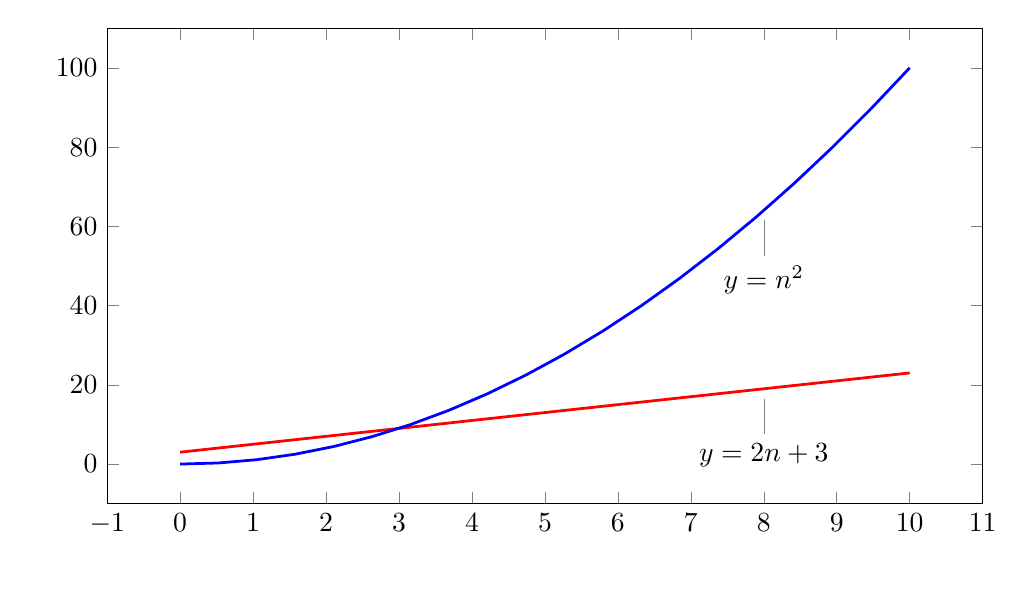
\begin{tikzpicture}[line width=1]
\begin{axis}[width=5in, height=3in,
             scatter/classes={a={mark=*,draw=black}},
             xlabel={\mbox{}},
             xlabel style={name=xlabel}, 
             ylabel={\mbox{}}, 
             legend style={
                at={(xlabel.south)},
                yshift=-1ex,
                anchor=north,
                legend cell align=left,
                },
        ]
]
\addplot[draw=red, line width=1] coordinates {(0.0,3.0)
(0.101,3.202)
(0.202,3.404)
(0.303,3.6061)
(0.404,3.8081)
(0.5051,4.0101)
(0.6061,4.2121)
(0.7071,4.4141)
(0.8081,4.6162)
(0.9091,4.8182)
(1.0101,5.0202)
(1.1111,5.2222)
(1.2121,5.4242)
(1.3131,5.6263)
(1.4141,5.8283)
(1.5152,6.0303)
(1.6162,6.2323)
(1.7172,6.4343)
(1.8182,6.6364)
(1.9192,6.8384)
(2.0202,7.0404)
(2.1212,7.2424)
(2.2222,7.4444)
(2.3232,7.6465)
(2.4242,7.8485)
(2.5253,8.0505)
(2.6263,8.2525)
(2.7273,8.4545)
(2.8283,8.6566)
(2.9293,8.8586)
(3.0303,9.0606)
(3.1313,9.2626)
(3.2323,9.4646)
(3.3333,9.6667)
(3.4343,9.8687)
(3.5354,10.0707)
(3.6364,10.2727)
(3.7374,10.4747)
(3.8384,10.6768)
(3.9394,10.8788)
(4.0404,11.0808)
(4.1414,11.2828)
(4.2424,11.4848)
(4.3434,11.6869)
(4.4444,11.8889)
(4.5455,12.0909)
(4.6465,12.2929)
(4.7475,12.4949)
(4.8485,12.697)
(4.9495,12.899)
(5.0505,13.101)
(5.1515,13.303)
(5.2525,13.5051)
(5.3535,13.7071)
(5.4545,13.9091)
(5.5556,14.1111)
(5.6566,14.3131)
(5.7576,14.5152)
(5.8586,14.7172)
(5.9596,14.9192)
(6.0606,15.1212)
(6.1616,15.3232)
(6.2626,15.5253)
(6.3636,15.7273)
(6.4646,15.9293)
(6.5657,16.1313)
(6.6667,16.3333)
(6.7677,16.5354)
(6.8687,16.7374)
(6.9697,16.9394)
(7.0707,17.1414)
(7.1717,17.3434)
(7.2727,17.5455)
(7.3737,17.7475)
(7.4747,17.9495)
(7.5758,18.1515)
(7.6768,18.3535)
(7.7778,18.5556)
(7.8788,18.7576)
(7.9798,18.9596)
(8.0808,19.1616)
(8.1818,19.3636)
(8.2828,19.5657)
(8.3838,19.7677)
(8.4848,19.9697)
(8.5859,20.1717)
(8.6869,20.3737)
(8.7879,20.5758)
(8.8889,20.7778)
(8.9899,20.9798)
(9.0909,21.1818)
(9.1919,21.3838)
(9.2929,21.5859)
(9.3939,21.7879)
(9.4949,21.9899)
(9.596,22.1919)
(9.697,22.3939)
(9.798,22.596)
(9.899,22.798)
(10.0,23.0)
(10.0,23.0)};\node[pin=below:{$y=2 n+3$}] at (axis cs:8.0,19.0) {};\addplot[draw=blue, line width=1] coordinates {(0.0,0.0)
(0.5263,0.277)
(1.0526,1.108)
(1.5789,2.4931)
(2.1053,4.4321)
(2.6316,6.9252)
(3.1579,9.9723)
(3.6842,13.5734)
(4.2105,17.7285)
(4.7368,22.4377)
(5.2632,27.7008)
(5.7895,33.518)
(6.3158,39.8892)
(6.8421,46.8144)
(7.3684,54.2936)
(7.8947,62.3269)
(8.4211,70.9141)
(8.9474,80.0554)
(9.4737,89.7507)
(10.0,100.0)};\node[pin=below:{$y=n^2$}] at (axis cs:8.0,64.0) {};
\end{axis}\end{tikzpicture}\end{center}

You see that 
\[
f(n) \leq g(n) \text{ for $n \geq 3$}
\]
If I choose $C = 1$ and $N = 3$, then for $n \geq N = 3$, 
we have (from the graph):
\[
f(n) \leq Cg(n)
\]
So we say that 
\[
f(n) = O(g(n))
\]
Note that the choice of $C$ and $N$ is not unique.
You can also choose $C = 2, N = 10$.

Here's another example.

Suppose
\[
f(n) = 3n^2 + 5 + 10 n \sin (n)
\]
Here's the plot:
\input{definition_of_big_O_3.tex}
For this example $f(n)$ is positive so $|f(n)| = f(n)$.
Let's see if we can \textit{cap} it with 
\[
g(n) = n
\]
%-*-latex-*-

\begin{center}
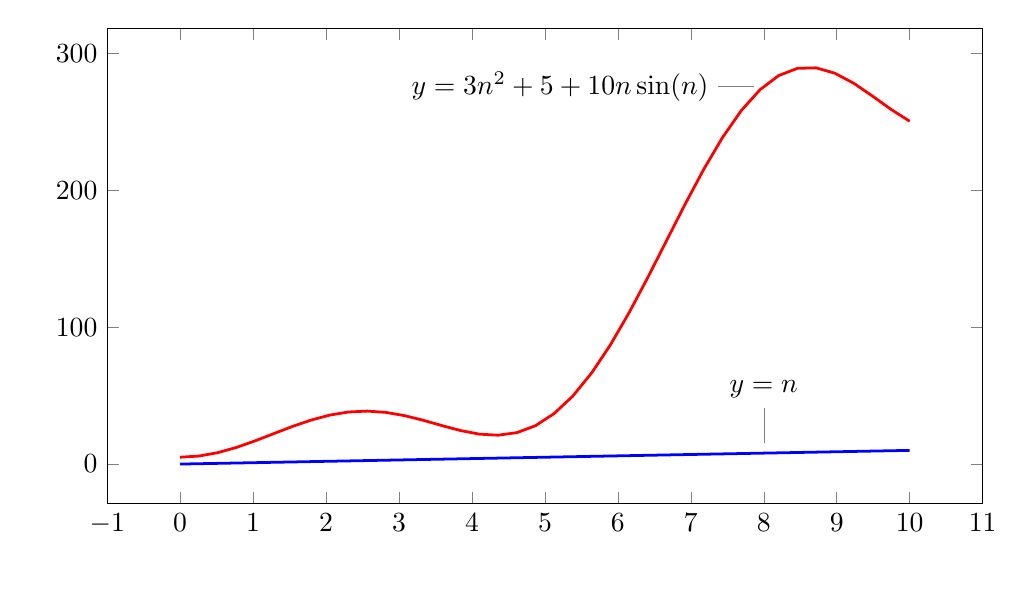
\begin{tikzpicture}[line width=1]
\begin{axis}[width=5in, height=3in,
             scatter/classes={a={mark=*,draw=black}},
             xlabel={\mbox{}},
             xlabel style={name=xlabel}, 
             ylabel={\mbox{}}, 
             legend style={
                at={(xlabel.south)},
                yshift=-1ex,
                anchor=north,
                legend cell align=left,
                },
        ]
]
\addplot[draw=red, line width=1] coordinates {(0.0,5.0)
(0.2564,5.8475)
(0.5128,8.305)
(0.7692,12.1258)
(1.0256,16.9255)
(1.2821,22.2207)
(1.5385,27.4772)
(1.7949,32.1647)
(2.0513,35.8134)
(2.3077,38.0661)
(2.5641,38.7219)
(2.8205,37.7672)
(3.0769,35.3908)
(3.3333,31.9811)
(3.5897,28.1044)
(3.8462,24.4672)
(4.1026,21.8624)
(4.359,21.1062)
(4.6154,22.9685)
(4.8718,28.1029)
(5.1282,36.9833)
(5.3846,49.851)
(5.641,66.6779)
(5.8974,87.1499)
(6.1538,110.6723)
(6.4103,136.3978)
(6.6667,163.2767)
(6.9231,190.1253)
(7.1795,215.7085)
(7.4359,238.832)
(7.6923,258.4347)
(7.9487,273.6771)
(8.2051,284.0168)
(8.4615,289.266)
(8.7179,289.6245)
(8.9744,285.6866)
(9.2308,278.4177)
(9.4872,269.1034)
(9.7436,259.2725)
(10.0,250.5979)
(10.0,250.5979)};\node[pin=left:{$y=3 n^2 + 5 + 10 n   \sin(n)$}] at (axis cs:8.0,276.14865972987053) {};\addplot[draw=blue, line width=1] coordinates {(0.0,0.0)
(5.0,5.0)
(10.0,10.0)
(10.0,10.0)};\node[pin=above:{$y=n$}] at (axis cs:8.0,8.0) {};
\end{axis}\end{tikzpicture}\end{center}

Not good.
But don't forget that if we do want to say $f(n) = O(g(n))$,
then we are allowed to use multiples of $g(n)$.
So let's try
\[
10g(n) = 10 n
\]
%-*-latex-*-

\begin{center}
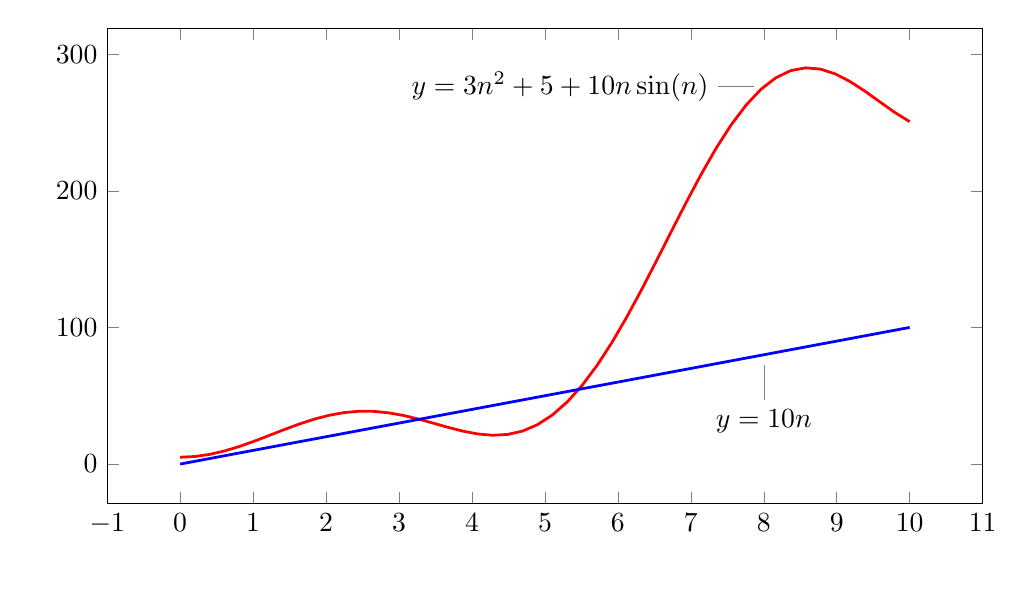
\begin{tikzpicture}[line width=1]
\begin{axis}[width=5in, height=3in,
             scatter/classes={a={mark=*,draw=black}},
             xlabel={\mbox{}},
             xlabel style={name=xlabel}, 
             ylabel={\mbox{}}, 
             legend style={
                at={(xlabel.south)},
                yshift=-1ex,
                anchor=north,
                legend cell align=left,
                },
        ]
]
\addplot[draw=red, line width=1] coordinates {(0.0,5.0)
(0.2041,5.5386)
(0.4082,7.1199)
(0.6122,9.6431)
(0.8163,12.9472)
(1.0204,16.8209)
(1.2245,21.0161)
(1.4286,25.2639)
(1.6327,29.292)
(1.8367,32.8424)
(2.0408,35.6899)
(2.2449,37.6574)
(2.449,38.6305)
(2.6531,38.5678)
(2.8571,37.5078)
(3.0612,35.5709)
(3.2653,32.9573)
(3.4694,29.94)
(3.6735,26.8531)
(3.8776,24.0763)
(4.0816,22.0167)
(4.2857,21.0872)
(4.4898,21.6846)
(4.6939,24.1667)
(4.898,28.8313)
(5.102,35.8965)
(5.3061,45.4846)
(5.5102,57.6108)
(5.7143,72.176)
(5.9184,88.9657)
(6.1224,107.6545)
(6.3265,127.8164)
(6.5306,148.9408)
(6.7347,170.4534)
(6.9388,191.7405)
(7.1429,212.1775)
(7.3469,231.1583)
(7.551,248.125)
(7.7551,262.597)
(7.9592,274.1976)
(8.1633,282.676)
(8.3673,287.9252)
(8.5714,289.9927)
(8.7755,289.0858)
(8.9796,285.5677)
(9.1837,279.9479)
(9.3878,272.8647)
(9.5918,265.0604)
(9.7959,257.3524)
(10.0,250.5979)
(10.0,250.5979)};\node[pin=left:{$y=3 n^2 + 5 + 10 n   \sin(n)$}] at (axis cs:8.0,276.14865972987053) {};\addplot[draw=blue, line width=1] coordinates {(0.0,0.0)
(5.0,50.0)
(10.0,100.0)
(10.0,100.0)};\node[pin=below:{$y=10 n$}] at (axis cs:8.0,80.0) {};
\end{axis}\end{tikzpicture}\end{center}


Better!!!
But just by looking at the graph,
my multiple of $g(n)$ must at least 
overcome the bump of $f(n)$ at around $n=8.5$.
Let's try 
\[
30g(n) = 30 n
\]
\input{definition_of_big_O_37.tex}

Finally let's try
\[
50g(n) = 50n
\]
\input{definition_of_big_O_6.tex}

The picture is not that clear for small $n$ values.
So let's zoom in near $n = 0$ and see how $50n$ performs
against $f(n)$:
%-*-latex-*-

\begin{center}
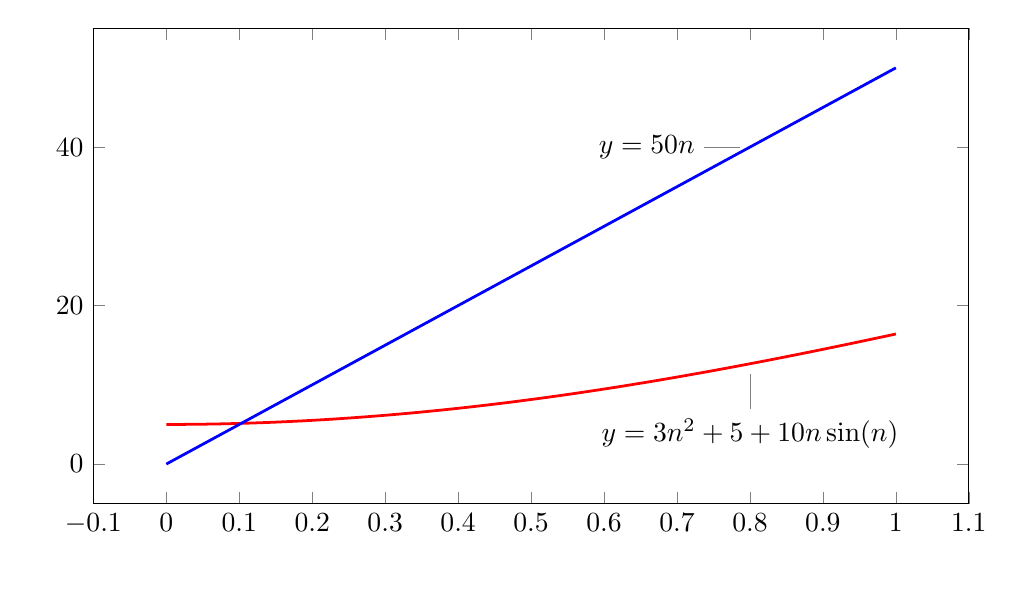
\begin{tikzpicture}[line width=1]
\begin{axis}[width=5in, height=3in,
             scatter/classes={a={mark=*,draw=black}},
             xlabel={\mbox{}},
             xlabel style={name=xlabel}, 
             ylabel={\mbox{}}, 
             legend style={
                at={(xlabel.south)},
                yshift=-1ex,
                anchor=north,
                legend cell align=left,
                },
        ]
]
\addplot[draw=red, line width=1] coordinates {(0.0,5.0)
(0.0101,5.0013)
(0.0202,5.0053)
(0.0303,5.0119)
(0.0404,5.0212)
(0.0505,5.0331)
(0.0606,5.0477)
(0.0707,5.065)
(0.0808,5.0848)
(0.0909,5.1073)
(0.101,5.1325)
(0.1111,5.1602)
(0.1212,5.1906)
(0.1313,5.2237)
(0.1414,5.2593)
(0.1515,5.2976)
(0.1616,5.3384)
(0.1717,5.3819)
(0.1818,5.4279)
(0.1919,5.4766)
(0.202,5.5278)
(0.2121,5.5816)
(0.2222,5.6379)
(0.2323,5.6968)
(0.2424,5.7583)
(0.2525,5.8222)
(0.2626,5.8887)
(0.2727,5.9578)
(0.2828,6.0293)
(0.2929,6.1033)
(0.303,6.1798)
(0.3131,6.2587)
(0.3232,6.3401)
(0.3333,6.424)
(0.3434,6.5103)
(0.3535,6.599)
(0.3636,6.6901)
(0.3737,6.7835)
(0.3838,6.8794)
(0.3939,6.9776)
(0.404,7.0782)
(0.4141,7.1811)
(0.4242,7.2863)
(0.4343,7.3937)
(0.4444,7.5035)
(0.4545,7.6155)
(0.4646,7.7298)
(0.4747,7.8463)
(0.4848,7.965)
(0.4949,8.0859)
(0.5051,8.2089)
(0.5152,8.3341)
(0.5253,8.4615)
(0.5354,8.5909)
(0.5455,8.7224)
(0.5556,8.856)
(0.5657,8.9917)
(0.5758,9.1293)
(0.5859,9.269)
(0.596,9.4106)
(0.6061,9.5543)
(0.6162,9.6998)
(0.6263,9.8473)
(0.6364,9.9966)
(0.6465,10.1478)
(0.6566,10.3009)
(0.6667,10.4558)
(0.6768,10.6125)
(0.6869,10.7709)
(0.697,10.9311)
(0.7071,11.093)
(0.7172,11.2567)
(0.7273,11.4219)
(0.7374,11.5889)
(0.7475,11.7574)
(0.7576,11.9275)
(0.7677,12.0992)
(0.7778,12.2725)
(0.7879,12.4472)
(0.798,12.6234)
(0.8081,12.8011)
(0.8182,12.9802)
(0.8283,13.1607)
(0.8384,13.3426)
(0.8485,13.5258)
(0.8586,13.7103)
(0.8687,13.8961)
(0.8788,14.0832)
(0.8889,14.2715)
(0.899,14.4609)
(0.9091,14.6516)
(0.9192,14.8433)
(0.9293,15.0362)
(0.9394,15.2302)
(0.9495,15.4252)
(0.9596,15.6212)
(0.9697,15.8182)
(0.9798,16.0161)
(0.9899,16.215)
(1.0,16.4147)
(1.0,16.4147)};\node[pin=below:{$y=3 n^2+5+10 n \sin(n)$}] at (axis cs:0.8,12.658848727196183) {};\addplot[draw=blue, line width=1] coordinates {(0.0,0.0)
(0.5,25.0)
(1.0,50.0)
(1.0,50.0)};\node[pin=left:{$y=50 n$}] at (axis cs:0.8,40.0) {};
\end{axis}\end{tikzpicture}\end{center}

Clearly from the plot for $0 \leq n \leq 1$, we see that
$50g(n)$ beats $f(n)$ after 0.1.

So from the previous two graphs
can we say that for $n \geq 1$, $50g(n)$ beats $f(n)$? ... i.e.,
can we say
\[
f(n) \leq 50 g(n) \text{ for $n \geq 1$}
\]
and conclude that $f(n) = O(g(n))$?

NO!!!

The problem is that our graphs cannot show \textit{all}
large values of $n$.
In fact when we plot for $n$ up to 20, we see that trend changes:
%-*-latex-*-

\begin{center}
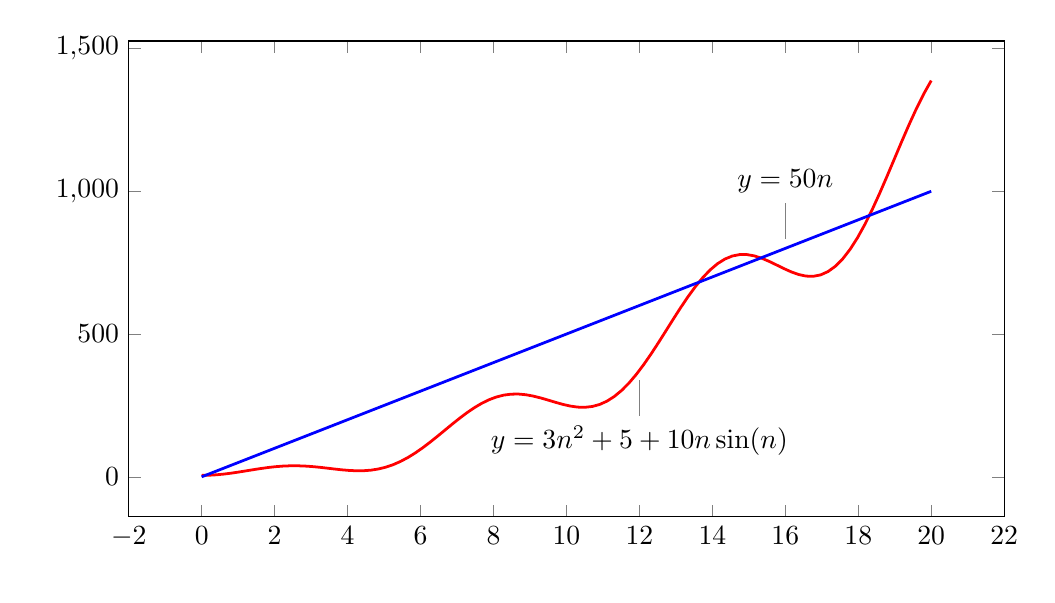
\begin{tikzpicture}[line width=1]
\begin{axis}[width=5in, height=3in,
             scatter/classes={a={mark=*,draw=black}},
             xlabel={\mbox{}},
             xlabel style={name=xlabel}, 
             ylabel={\mbox{}}, 
             legend style={
                at={(xlabel.south)},
                yshift=-1ex,
                anchor=north,
                legend cell align=left,
                },
        ]
]
\addplot[draw=red, line width=1] coordinates {(0.0,5.0)
(0.202,5.5278)
(0.404,7.0782)
(0.6061,9.5543)
(0.8081,12.8011)
(1.0101,16.6153)
(1.2121,20.7576)
(1.4141,24.9676)
(1.6162,28.9809)
(1.8182,32.5456)
(2.0202,35.4397)
(2.2222,37.4864)
(2.4242,38.5676)
(2.6263,38.6346)
(2.8283,37.7146)
(3.0303,35.9137)
(3.2323,33.4151)
(3.4343,30.4731)
(3.6364,27.4029)
(3.8384,24.5664)
(4.0404,22.3549)
(4.2424,21.1697)
(4.4444,21.4007)
(4.6465,23.4052)
(4.8485,27.4869)
(5.0505,33.8773)
(5.2525,42.7194)
(5.4545,54.0555)
(5.6566,67.8195)
(5.8586,83.8343)
(6.0606,101.8143)
(6.2626,121.374)
(6.4646,142.0415)
(6.6667,163.2767)
(6.8687,184.4941)
(7.0707,205.0882)
(7.2727,224.4613)
(7.4747,242.0521)
(7.6768,257.3637)
(7.8788,269.9895)
(8.0808,279.6366)
(8.2828,286.1436)
(8.4848,289.4945)
(8.6869,289.8253)
(8.8889,287.4242)
(9.0909,282.7249)
(9.2929,276.2927)
(9.4949,268.8049)
(9.697,261.024)
(9.899,253.7675)
(10.101,247.8732)
(10.303,244.1627)
(10.5051,243.4047)
(10.7071,246.2785)
(10.9091,253.3416)
(11.1111,265.0)
(11.3131,281.486)
(11.5152,302.8413)
(11.7172,328.9095)
(11.9192,359.3361)
(12.1212,393.5773)
(12.3232,430.918)
(12.5253,470.4972)
(12.7273,511.3406)
(12.9293,552.3998)
(13.1313,592.5949)
(13.3333,630.8602)
(13.5354,666.1907)
(13.7374,697.687)
(13.9394,724.5968)
(14.1414,746.3516)
(14.3434,762.5962)
(14.5455,773.2092)
(14.7475,778.3154)
(14.9495,778.2864)
(15.1515,773.7315)
(15.3535,765.4782)
(15.5556,754.5421)
(15.7576,742.0891)
(15.9596,729.389)
(16.1616,717.7649)
(16.3636,708.5379)
(16.5657,702.971)
(16.7677,702.2147)
(16.9697,707.2553)
(17.1717,718.8693)
(17.3737,737.5859)
(17.5758,763.659)
(17.7778,797.0499)
(17.9798,837.4227)
(18.1818,884.1517)
(18.3838,936.3413)
(18.5859,992.858)
(18.7879,1052.3727)
(18.9899,1113.4124)
(19.1919,1174.4193)
(19.3939,1233.8141)
(19.596,1290.062)
(19.798,1341.7381)
(20.0,1387.5891)
(20.0,1387.5891)};\node[pin=below:{$y=3 n^2 + 5 + 10 n   \sin(n)$}] at (axis cs:12,372.6112498399478) {};\addplot[draw=blue, line width=1] coordinates {(0.0,0.0)
(10.0,500.0)
(20.0,1000.0)
(20.0,1000.0)};\node[pin=above:{$y=50 n$}] at (axis cs:16.0,800.0) {};
\end{axis}\end{tikzpicture}\end{center}


It's even more revealing when I plot up to $n = 100$:
%-*-latex-*-

\begin{center}
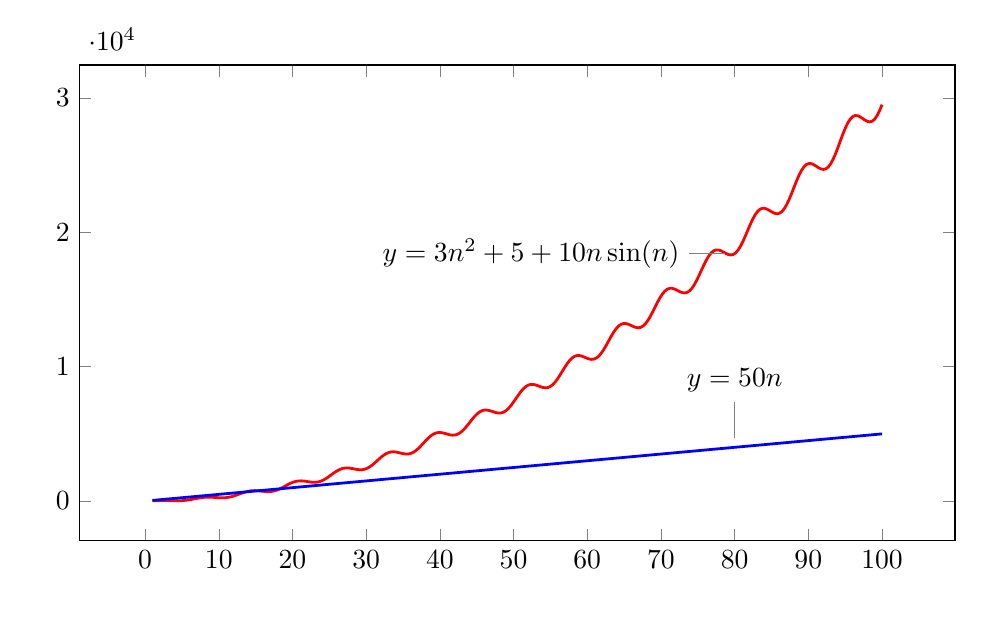
\begin{tikzpicture}[line width=1]
\begin{axis}[width=5in, height=3in,
             scatter/classes={a={mark=*,draw=black}},
             xlabel={\mbox{}},
             xlabel style={name=xlabel}, 
             ylabel={\mbox{}}, 
             legend style={
                at={(xlabel.south)},
                yshift=-1ex,
                anchor=north,
                legend cell align=left,
                },
        ]
]
\addplot[draw=red, line width=1] coordinates {(1.0,16.4147)
(1.3311,23.246)
(1.6622,29.8415)
(1.9933,35.1001)
(2.3244,38.1588)
(2.6555,38.5608)
(2.9866,36.3696)
(3.3177,32.2085)
(3.6488,27.2172)
(3.9799,22.9274)
(4.311,21.0706)
(4.6421,23.3415)
(4.9732,31.1495)
(5.3043,45.3902)
(5.6355,66.2717)
(5.9666,93.2215)
(6.2977,124.893)
(6.6288,159.2757)
(6.9599,193.9025)
(7.291,226.1309)
(7.6221,253.4683)
(7.9532,273.8999)
(8.2843,286.1789)
(8.6154,290.0386)
(8.9465,286.2962)
(9.2776,276.8272)
(9.6087,264.4085)
(9.9398,252.44)
(10.2709,244.5743)
(10.602,244.2931)
(10.9331,254.4808)
(11.2642,277.0456)
(11.5953,312.6371)
(11.9264,360.4994)
(12.2575,418.4829)
(12.5886,483.2225)
(12.9197,550.4677)
(13.2508,615.5336)
(13.5819,673.824)
(13.913,721.369)
(14.2441,755.3143)
(14.5753,774.3023)
(14.9064,778.6968)
(15.2375,770.6174)
(15.5686,753.7729)
(15.8997,733.1044)
(16.2308,714.2712)
(16.5619,703.0344)
(16.893,704.6039)
(17.2241,723.0234)
(17.5552,760.666)
(17.8863,817.9004)
(18.2174,892.9748)
(18.5485,982.1375)
(18.8796,1079.9888)
(19.2107,1180.0337)
(19.5418,1275.3762)
(19.8729,1359.4841)
(20.204,1426.937)
(20.5351,1474.0734)
(20.8662,1499.4602)
(21.1973,1504.125)
(21.5284,1491.5191)
(21.8595,1467.2052)
(22.1906,1438.2985)
(22.5217,1412.7166)
(22.8528,1398.3163)
(23.1839,1402.0133)
(23.5151,1428.9808)
(23.8462,1482.0218)
(24.1773,1561.1895)
(24.5084,1663.7048)
(24.8395,1784.1886)
(25.1706,1915.1916)
(25.5017,2047.9696)
(25.8328,2173.4231)
(26.1639,2283.1017)
(26.495,2370.1611)
(26.8261,2430.1658)
(27.1572,2461.642)
(27.4883,2466.3152)
(27.8194,2448.9965)
(28.1505,2417.1226)
(28.4816,2379.9931)
(28.8127,2347.7818)
(29.1438,2330.4288)
(29.4749,2336.5322)
(29.806,2372.3642)
(30.1371,2441.1239)
(30.4682,2542.5138)
(30.7993,2672.6959)
(31.1304,2824.6395)
(31.4615,2988.8304)
(31.7926,3154.2714)
(32.1237,3309.6668)
(32.4548,3444.6666)
(32.786,3551.0301)
(33.1171,3623.5801)
(33.4482,3660.8376)
(33.7793,3665.2593)
(34.1104,3643.0444)
(34.4415,3603.5238)
(34.7726,3558.1905)
(35.1037,3519.473)
(35.4348,3499.3807)
(35.7659,3508.1711)
(36.097,3553.1852)
(36.4281,3637.9833)
(36.7592,3761.8824)
(37.0903,3919.9547)
(37.4214,4103.4933)
(37.7525,4300.9046)
(38.0836,4498.9346)
(38.4147,4684.0998)
(38.7458,4844.1692)
(39.0769,4969.5328)
(39.408,5054.3051)
(39.7391,5097.0368)
(40.0702,5100.9493)
(40.4013,5073.658)
(40.7324,5026.4074)
(41.0635,4972.8934)
(41.3946,4927.796)
(41.7258,4905.1807)
(42.0569,4916.9409)
(42.388,4971.4553)
(42.7191,5072.6108)
(43.0502,5219.3046)
(43.3813,5405.4876)
(43.7124,5620.7531)
(44.0435,5851.4134)
(44.3746,6081.9549)
(44.7057,6296.7146)
(45.0368,6481.5994)
(45.3679,6625.6579)
(45.699,6722.3293)
(46.0301,6770.2294)
(46.3612,6773.3774)
(46.6923,6740.8326)
(47.0234,6685.7726)
(47.3545,6624.1044)
(47.6856,6572.7571)
(48.0167,6547.8379)
(48.3478,6562.8523)
(48.6789,6627.1857)
(49.01,6745.0173)
(49.3411,6914.7894)
(49.6722,7129.301)
(50.0033,7376.4217)
(50.3344,7640.356)
(50.6656,7903.3278)
(50.9967,8147.5034)
(51.3278,8356.9472)
(51.6589,8519.3941)
(51.99,8627.6416)
(52.3211,8680.4054)
(52.6522,8682.5357)
(52.9833,8644.5636)
(53.3144,8581.6182)
(53.6455,8511.8262)
(53.9766,8454.3625)
(54.3077,8427.3613)
(54.6388,8445.916)
(54.9699,8520.3881)
(55.301,8655.2136)
(55.6321,8848.3458)
(55.9632,9091.4011)
(56.2943,9370.5019)
(56.6254,9667.7314)
(56.9565,9963.0486)
(57.2876,10236.4584)
(57.6187,10470.2026)
(57.9498,10650.7302)
(58.2809,10770.2306)
(58.612,10827.5547)
(58.9431,10828.4167)
(59.2742,10784.8464)
(59.6054,10713.9433)
(59.9365,10636.0618)
(60.2676,10572.6185)
(60.5987,10543.7599)
(60.9298,10566.1431)
(61.2609,10651.0737)
(61.592,10803.2105)
(61.9231,11019.9828)
(62.2542,11291.7941)
(62.5853,11602.9965)
(62.9164,11933.5386)
(63.2475,12261.1127)
(63.5786,12563.5719)
(63.9097,12821.3553)
(64.2408,13019.6548)
(64.5719,13150.0851)
(64.903,13211.6674)
(65.2341,13211.0126)
(65.5652,13161.6765)
(65.8963,13082.7473)
(66.2274,12996.8141)
(66.5585,12927.5314)
(66.8896,12897.0429)
(67.2207,12923.5443)
(67.5518,13019.2541)
(67.8829,13189.0188)
(68.214,13429.7094)
(68.5452,13730.4861)
(68.8763,14073.908)
(69.2074,14437.7763)
(69.5385,14797.5151)
(69.8696,15128.8358)
(70.2007,15410.3952)
(70.5318,15626.1567)
(70.8629,15767.1939)
(71.194,15832.7334)
(71.5251,15830.316)
(71.8562,15775.0498)
(72.1873,15688.0295)
(72.5184,15594.0863)
(72.8495,15519.108)
(73.1806,15487.2196)
(73.5117,15518.1305)
(73.8428,15624.9407)
(74.1739,15812.6491)
(74.505,16077.5342)
(74.8361,16407.4829)
(75.1672,16783.2388)
(75.4983,17180.4432)
(75.8294,17572.251)
(76.1605,17932.2422)
(76.4916,18237.3121)
(76.8227,18470.2244)
(77.1538,18621.5457)
(77.4849,18690.7431)
(77.8161,18686.3194)
(78.1472,18624.9619)
(78.4783,18529.7894)
(78.8094,18427.8816)
(79.1405,18347.3547)
(79.4716,18314.2992)
(79.8027,18349.9128)
(80.1338,18468.145)
(80.4649,18674.1121)
(80.796,18963.4661)
(81.1271,19322.7904)
(81.4582,19730.9913)
(81.7893,20161.5379)
(82.1204,20585.3153)
(82.4515,20973.7829)
(82.7826,21302.0956)
(83.1137,21551.8467)
(83.4448,21713.1294)
(83.7759,21785.6865)
(84.107,21779.0155)
(84.4381,21711.4088)
(84.7692,21608.0267)
(85.1003,21498.2034)
(85.4314,21412.2784)
(85.7625,21378.291)
(86.0936,21418.9022)
(86.4247,21548.8782)
(86.7559,21773.4185)
(87.087,22087.5136)
(87.4181,22476.4144)
(87.7492,22917.1677)
(88.0803,23381.0589)
(88.4114,23836.7028)
(88.7425,24253.4496)
(89.0736,24604.7354)
(89.4047,24871.0121)
(89.7358,25041.9337)
(90.0669,25117.5539)
(90.398,25108.3969)
(90.7291,25034.3866)
(91.0602,24922.7409)
(91.3913,24805.0551)
(91.7224,24713.8858)
(92.0535,24679.2047)
(92.3846,24725.1096)
(92.7157,24867.152)
(93.0468,25110.5787)
(93.3779,25449.6853)
(93.709,25868.3606)
(94.0401,26341.7701)
(94.3712,26839.0043)
(94.7023,27326.4083)
(95.0334,27771.2343)
(95.3645,28145.2211)
(95.6957,28427.7092)
(96.0268,28607.9477)
(96.3579,28686.3357)
(96.689,28674.4567)
(97.0201,28593.8913)
(97.3512,28473.932)
(97.6823,28348.4403)
(98.0134,28252.1838)
(98.3445,28217.0496)
(98.6756,28268.5461)
(99.0067,28422.9776)
(99.3378,28685.6033)
(99.6689,29049.9898)
(100.0,29498.6344)
(100.0,29498.6344)};\node[pin=left:{$y=3 n^2 + 5 + 10 n   \sin(n)$}] at (axis cs:80.0,18409.8890768613) {};\addplot[draw=blue, line width=1] coordinates {(1.0,50.0)
(50.5,2525.0)
(100.0,5000.0)
(100.0,5000.0)};\node[pin=above:{$y=50 n$}] at (axis cs:80.0,4000.0) {};
\end{axis}\end{tikzpicture}\end{center}


Clearly \textit{no} straight line is going to dominate $f(n)$ because
it seems that the graph of $f(n)$ \textit{bends} up (with wiggles along the way).

Here's an important advice:
\[
\text{\textit{GRAPHS ARE USEFUL TOOLS BUT THEY CAN DECEIVE!!!}}
\]

Let's see more of the graph to see if the pattern of bending
upward with wiggles persists.
Let's plot up to $n = 200$:
%-*-latex-*-

\begin{center}
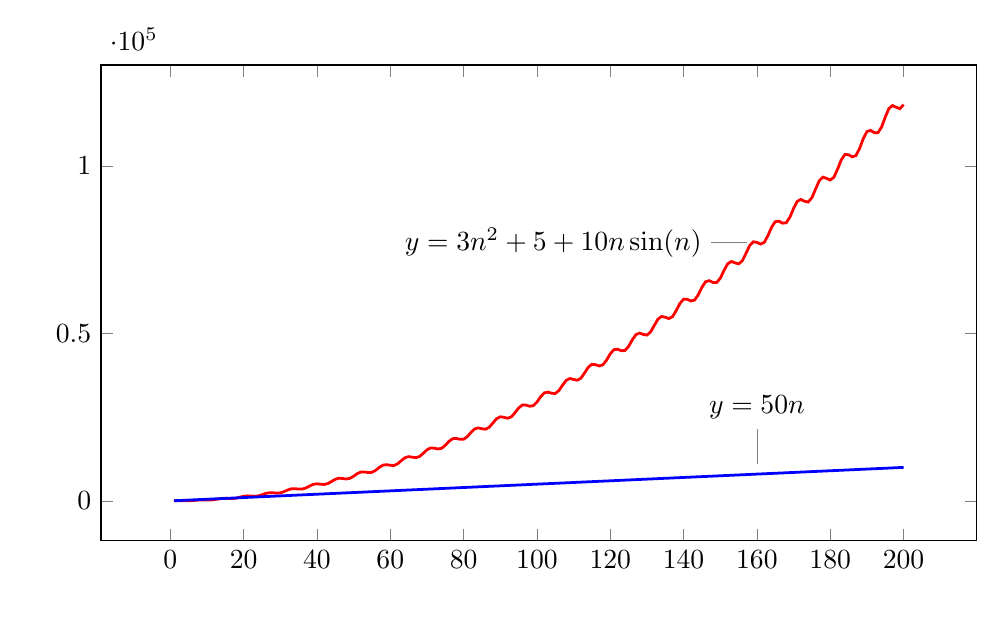
\begin{tikzpicture}[line width=1]
\begin{axis}[width=5in, height=3in,
             scatter/classes={a={mark=*,draw=black}},
             xlabel={\mbox{}},
             xlabel style={name=xlabel}, 
             ylabel={\mbox{}}, 
             legend style={
                at={(xlabel.south)},
                yshift=-1ex,
                anchor=north,
                legend cell align=left,
                },
        ]
]
\addplot[draw=red, line width=1] coordinates {(1.0,16.4147)
(2.0,35.1859)
(3.0,36.2336)
(4.0,22.7279)
(5.0,32.0538)
(6.0,96.2351)
(7.0,197.9891)
(8.0,276.1487)
(9.0,285.0907)
(10.0,250.5979)
(11.0,258.0011)
(12.0,372.6112)
(13.0,566.6217)
(14.0,731.685)
(15.0,777.5432)
(16.0,726.9355)
(17.0,708.5624)
(18.0,841.8223)
(19.0,1116.4767)
(20.0,1387.5891)
(21.0,1503.6977)
(22.0,1455.0527)
(23.0,1397.3693)
(24.0,1515.6612)
(25.0,1846.9121)
(26.0,2231.2652)
(27.0,2450.2215)
(28.0,2432.8536)
(29.0,2335.5462)
(30.0,2408.5905)
(31.0,2762.7483)
(32.0,3253.4565)
(33.0,3601.9709)
(34.0,3652.8881)
(35.0,3530.1361)
(36.0,3535.9596)
(37.0,3873.8909)
(38.0,4449.6201)
(39.0,4943.8802)
(40.0,5103.0453)
(41.0,4982.9647)
(42.0,4912.0609)
(43.0,5194.3369)
(44.0,5820.7888)
(45.0,6462.9066)
(46.0,6767.8226)
(47.0,6690.0794)
(48.0,6548.2378)
(49.0,6740.6612)
(50.0,7373.8126)
(51.0,8149.8169)
(52.0,8630.0463)
(53.0,8641.8403)
(54.0,8451.2539)
(55.0,8530.1347)
(56.0,9120.9314)
(57.0,10000.6139)
(58.0,10672.8661)
(59.0,10823.6754)
(60.0,10622.1136)
(61.0,10578.6682)
(62.0,11078.708)
(63.0,12017.4341)
(64.0,12881.8167)
(65.0,13217.4386)
(66.0,13055.4762)
(67.0,12898.8016)
(68.0,13266.4092)
(69.0,14208.7985)
(70.0,15246.7235)
(71.0,15803.2488)
(72.0,15739.7528)
(73.0,15497.9565)
(74.0,15703.9918)
(75.0,16589.1638)
(76.0,17763.2418)
(77.0,18561.6305)
(78.0,18657.9032)
(79.0,18377.151)
(80.0,18409.8891)
(81.0,19177.7907)
(82.0,20433.8476)
(83.0,21475.7425)
(84.0,21788.8799)
(85.0,21530.3357)
(86.0,21398.8257)
(87.0,21997.0185)
(88.0,23268.1505)
(89.0,24533.4618)
(90.0,25109.597)
(91.0,24944.4486)
(92.0,24679.8912)
(93.0,25070.0976)
(94.0,26282.4631)
(95.0,27729.0986)
(96.0,28597.2442)
(97.0,28600.2195)
(98.0,28255.0858)
(99.0,28418.7852)
(100.0,29498.6344)
(101.0,31064.546)
(102.0,32231.7233)
(103.0,32473.6783)
(104.0,32118.5127)
(105.0,32060.938)
(106.0,32942.2289)
(107.0,34549.7165)
(108.0,35997.964)
(109.0,36538.2494)
(110.0,36256.3331)
(111.0,36008.3479)
(112.0,36640.2049)
(113.0,38202.1844)
(114.0,39887.8776)
(115.0,40767.2506)
(116.0,40647.5272)
(117.0,40265.0534)
(118.0,40618.2964)
(119.0,42046.0291)
(120.0,43901.7334)
(121.0,45136.5664)
(122.0,45265.43)
(123.0,44826.3187)
(124.0,44898.3481)
(125.0,46109.9494)
(126.0,48048.7884)
(127.0,49627.2402)
(128.0,50079.9283)
(129.0,49678.4193)
(130.0,49495.8623)
(131.0,50424.7996)
(132.0,52347.0703)
(133.0,54227.7245)
(134.0,55060.1393)
(135.0,54799.2977)
(136.0,54418.0108)
(137.0,55020.7552)
(138.0,56822.2879)
(139.0,58935.5514)
(140.0,60177.3355)
(141.0,60160.0716)
(142.0,59662.3311)
(143.0,59924.3661)
(144.0,61505.9289)
(145.0,63758.2305)
(146.0,65407.845)
(147.0,65727.2947)
(148.0,65216.2666)
(149.0,65155.7735)
(150.0,66432.6854)
(151.0,68713.2463)
(152.0,70735.6472)
(153.0,71465.7929)
(154.0,71057.6427)
(155.0,70726.3664)
(156.0,71637.416)
(157.0,73827.1088)
(158.0,76154.4021)
(159.0,77341.8364)
(160.0,77156.0804)
(161.0,76637.1235)
(162.0,77151.9104)
(163.0,79133.4964)
(164.0,81668.6898)
(165.0,83326.3655)
(166.0,83475.264)
(167.0,82877.8312)
(168.0,83001.7489)
(169.0,84670.6202)
(170.0,87294.3041)
(171.0,89397.9704)
(172.0,89975.8937)
(173.0,89427.2978)
(174.0,89203.5562)
(175.0,90478.0145)
(176.0,93057.5239)
(177.0,95545.3339)
(178.0,96619.0841)
(179.0,96254.5927)
(180.0,95762.9253)
(181.0,96593.023)
(182.0,98993.3785)
(183.0,101768.8851)
(184.0,103369.9153)
(185.0,103321.2492)
(186.0,102673.2355)
(187.0,103047.2902)
(188.0,105143.0155)
(189.0,108081.4709)
(190.0,110200.8186)
(191.0,110584.2753)
(192.0,109915.5184)
(193.0,109863.5788)
(194.0,111550.3705)
(195.0,114507.9366)
(196.0,117094.4789)
(197.0,117999.7375)
(198.0,117459.4344)
(199.0,117053.2203)
(200.0,118258.4054)
(200.0,118258.4054)};\node[pin=left:{$y=3 n^2 + 5 + 10 n   \sin(n)$}] at (axis cs:160.0,77156.08041340641) {};\addplot[draw=blue, line width=1] coordinates {(1.0,50.0)
(100.5,5025.0)
(200.0,10000.0)
(200.0,10000.0)};\node[pin=above:{$y=50 n$}] at (axis cs:160.0,8000.0) {};
\end{axis}\end{tikzpicture}\end{center}


So let's abandon our $g(n) = n$ altogether.

What should we use to chase $f(n)$?
Of course you know that $g(n) = n^2$ is a parabola and bends up.
But does it increase (or bends) fast enough?
If you look at 
\[
f(n) = 3n^2 + 5 + 10 n \sin (n)
\]
You see that it is made up of three functions:
$3n^2$, $5$, and $10n \sin n$.
Of course $3n^2$ is going to beat $5$.
So the growth of $3n^2 + 5$ is primarily determined by $3n^2$.
Let's look at them together in a graph:
%-*-latex-*-

\begin{center}
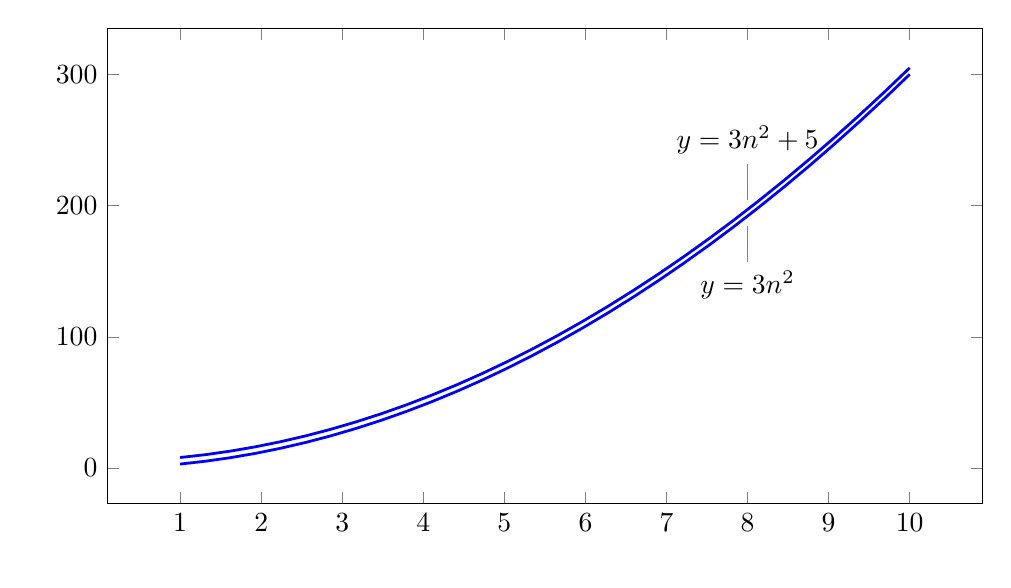
\begin{tikzpicture}[line width=1]
\begin{axis}[width=5in, height=3in,
             scatter/classes={a={mark=*,draw=black}},
             xlabel={\mbox{}},
             xlabel style={name=xlabel}, 
             ylabel={\mbox{}}, 
             legend style={
                at={(xlabel.south)},
                yshift=-1ex,
                anchor=north,
                legend cell align=left,
                },
        ]
]
\addplot[draw=blue, line width=1] coordinates {(1.0,3.0)
(1.3103,5.151)
(1.6207,7.8799)
(1.931,11.1867)
(2.2414,15.0713)
(2.5517,19.5339)
(2.8621,24.5743)
(3.1724,30.1926)
(3.4828,36.3888)
(3.7931,43.1629)
(4.1034,50.5149)
(4.4138,58.4447)
(4.7241,66.9524)
(5.0345,76.038)
(5.3448,85.7015)
(5.6552,95.9429)
(5.9655,106.7622)
(6.2759,118.1593)
(6.5862,130.1344)
(6.8966,142.6873)
(7.2069,155.8181)
(7.5172,169.5268)
(7.8276,183.8133)
(8.1379,198.6778)
(8.4483,214.1201)
(8.7586,230.1403)
(9.069,246.7384)
(9.3793,263.9144)
(9.6897,281.6683)
(10.0,300.0)};\node[pin=below:{$y=3 n^2$}] at (axis cs:8.0,192.0) {};\addplot[draw=blue, line width=1] coordinates {(1.0,8.0)
(1.3103,10.151)
(1.6207,12.8799)
(1.931,16.1867)
(2.2414,20.0713)
(2.5517,24.5339)
(2.8621,29.5743)
(3.1724,35.1926)
(3.4828,41.3888)
(3.7931,48.1629)
(4.1034,55.5149)
(4.4138,63.4447)
(4.7241,71.9524)
(5.0345,81.038)
(5.3448,90.7015)
(5.6552,100.9429)
(5.9655,111.7622)
(6.2759,123.1593)
(6.5862,135.1344)
(6.8966,147.6873)
(7.2069,160.8181)
(7.5172,174.5268)
(7.8276,188.8133)
(8.1379,203.6778)
(8.4483,219.1201)
(8.7586,235.1403)
(9.069,251.7384)
(9.3793,268.9144)
(9.6897,286.6683)
(10.0,305.0)};\node[pin=above:{$y=3 n^2 + 5$}] at (axis cs:8.0,197.0) {};
\end{axis}\end{tikzpicture}\end{center}

Of course since we can control $f(n)$ with multiples $g(n) = n^2$,
later we just need to choose a huge multiple of $n^2$ to 
beat $3n^2 + 5$, for instance $1000000 g(n) = 1000000 n^2$.

What about $10n \sin n$?
If we plot that with $3g(n) = 3n^2$ we get:
%-*-latex-*-

\begin{center}
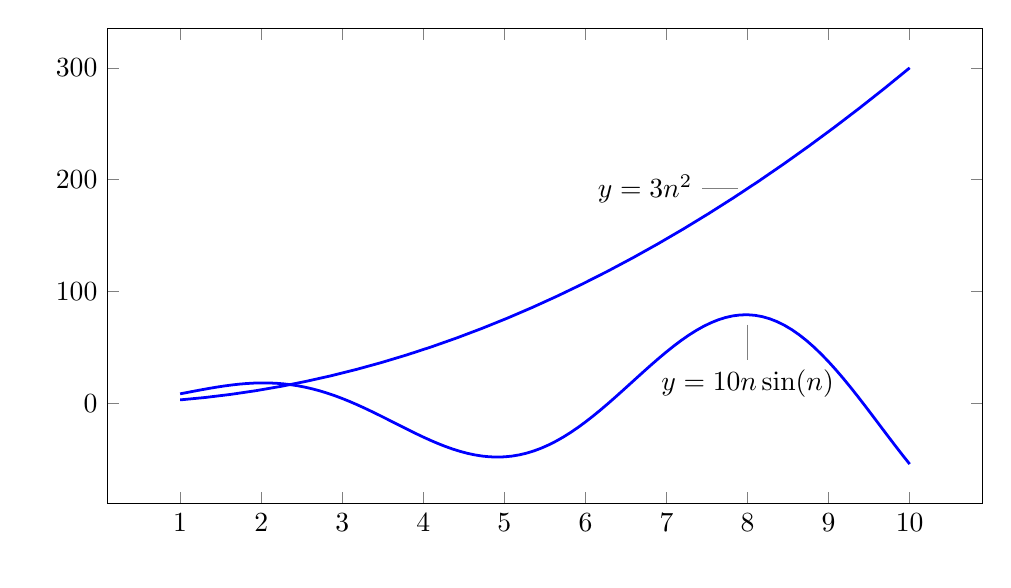
\begin{tikzpicture}[line width=1]
\begin{axis}[width=5in, height=3in,
             scatter/classes={a={mark=*,draw=black}},
             xlabel={\mbox{}},
             xlabel style={name=xlabel}, 
             ylabel={\mbox{}}, 
             legend style={
                at={(xlabel.south)},
                yshift=-1ex,
                anchor=north,
                legend cell align=left,
                },
        ]
]
\addplot[draw=blue, line width=1] coordinates {(1.0,3.0)
(1.3103,5.151)
(1.6207,7.8799)
(1.931,11.1867)
(2.2414,15.0713)
(2.5517,19.5339)
(2.8621,24.5743)
(3.1724,30.1926)
(3.4828,36.3888)
(3.7931,43.1629)
(4.1034,50.5149)
(4.4138,58.4447)
(4.7241,66.9524)
(5.0345,76.038)
(5.3448,85.7015)
(5.6552,95.9429)
(5.9655,106.7622)
(6.2759,118.1593)
(6.5862,130.1344)
(6.8966,142.6873)
(7.2069,155.8181)
(7.5172,169.5268)
(7.8276,183.8133)
(8.1379,198.6778)
(8.4483,214.1201)
(8.7586,230.1403)
(9.069,246.7384)
(9.3793,263.9144)
(9.6897,281.6683)
(10.0,300.0)};\node[pin=left:{$y=3 n^2$}] at (axis cs:8.0,192.0) {};\addplot[draw=blue, line width=1] coordinates {(1.0,8.4147)
(1.0909,9.6769)
(1.1818,10.9353)
(1.2727,12.1661)
(1.3636,13.3448)
(1.4545,14.4473)
(1.5455,15.4496)
(1.6364,16.3285)
(1.7273,17.0617)
(1.8182,17.6283)
(1.9091,18.0089)
(2.0,18.1859)
(2.0909,18.1441)
(2.1818,17.8704)
(2.2727,17.3545)
(2.3636,16.5886)
(2.4545,15.5681)
(2.5455,14.2915)
(2.6364,12.7602)
(2.7273,10.9791)
(2.8182,8.9562)
(2.9091,6.7029)
(3.0,4.2336)
(3.0909,1.5659)
(3.1818,-1.2796)
(3.2727,-4.2794)
(3.3636,-7.4075)
(3.4545,-10.6355)
(3.5455,-13.9327)
(3.6364,-17.2665)
(3.7273,-20.6031)
(3.8182,-23.9071)
(3.9091,-27.1423)
(4.0,-30.2721)
(4.0909,-33.2598)
(4.1818,-36.069)
(4.2727,-38.6637)
(4.3636,-41.0094)
(4.4545,-43.0729)
(4.5455,-44.8227)
(4.6364,-46.2297)
(4.7273,-47.2675)
(4.8182,-47.9124)
(4.9091,-48.1443)
(5.0,-47.9462)
(5.0909,-47.3054)
(5.1818,-46.2128)
(5.2727,-44.664)
(5.3636,-42.6585)
(5.4545,-40.2007)
(5.5455,-37.2993)
(5.6364,-33.9677)
(5.7273,-30.2239)
(5.8182,-26.0902)
(5.9091,-21.5936)
(6.0,-16.7649)
(6.0909,-11.6393)
(6.1818,-6.2556)
(6.2727,-0.656)
(6.3636,5.1141)
(6.4545,11.0065)
(6.5455,16.9706)
(6.6364,22.954)
(6.7273,28.9027)
(6.8182,34.7617)
(6.9091,40.4756)
(7.0,45.9891)
(7.0909,51.2471)
(7.1818,56.196)
(7.2727,60.7836)
(7.3636,64.9598)
(7.4545,68.6773)
(7.5455,71.8917)
(7.6364,74.5626)
(7.7273,76.6532)
(7.8182,78.1317)
(7.9091,78.9708)
(8.0,79.1487)
(8.0909,78.6488)
(8.1818,77.4606)
(8.2727,75.5796)
(8.3636,73.0073)
(8.4545,69.7514)
(8.5455,65.8263)
(8.6364,61.2522)
(8.7273,56.0559)
(8.8182,50.2702)
(8.9091,43.9336)
(9.0,37.0907)
(9.0909,29.791)
(9.1818,22.0893)
(9.2727,14.045)
(9.3636,5.7215)
(9.4545,-2.814)
(9.5455,-11.4912)
(9.6364,-20.2374)
(9.7273,-28.9778)
(9.8182,-37.6365)
(9.9091,-46.1368)
(10.0,-54.4021)};\node[pin=below:{$y=10   n   \sin(n)$}] at (axis cs:8.0,79.14865972987054) {};
\end{axis}\end{tikzpicture}\end{center}

To make sure that the pattern persists, I'm going to plot up
to $n = 100$:
%-*-latex-*-

\begin{center}
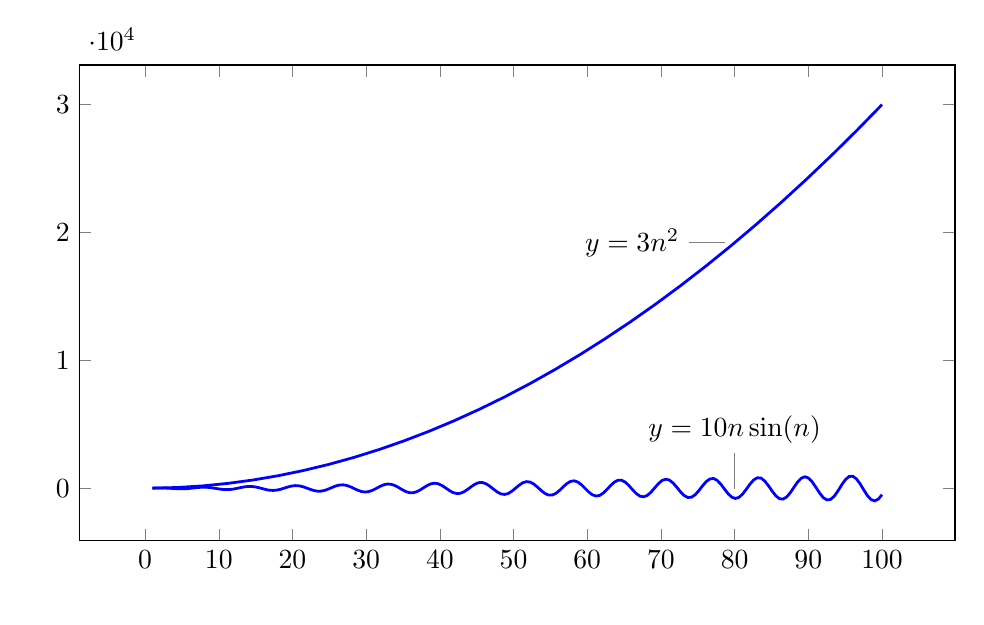
\begin{tikzpicture}[line width=1]
\begin{axis}[width=5in, height=3in,
             scatter/classes={a={mark=*,draw=black}},
             xlabel={\mbox{}},
             xlabel style={name=xlabel}, 
             ylabel={\mbox{}}, 
             legend style={
                at={(xlabel.south)},
                yshift=-1ex,
                anchor=north,
                legend cell align=left,
                },
        ]
]
\addplot[draw=blue, line width=1] coordinates {(1.0,3.0)
(4.4138,58.4447)
(7.8276,183.8133)
(11.2414,379.1058)
(14.6552,644.3222)
(18.069,979.4625)
(21.4828,1384.5268)
(24.8966,1859.5149)
(28.3103,2404.4269)
(31.7241,3019.2628)
(35.1379,3704.0226)
(38.5517,4458.7063)
(41.9655,5283.3139)
(45.3793,6177.8454)
(48.7931,7142.3008)
(52.2069,8176.6801)
(55.6207,9280.9834)
(59.0345,10455.2105)
(62.4483,11699.3615)
(65.8621,13013.4364)
(69.2759,14397.4352)
(72.6897,15851.3579)
(76.1034,17375.2045)
(79.5172,18968.975)
(82.931,20632.6694)
(86.3448,22366.2878)
(89.7586,24169.83)
(93.1724,26043.2961)
(96.5862,27986.6861)
(100.0,30000.0)
(100.0,30000.0)};\node[pin=left:{$y=3 n^2$}] at (axis cs:80.0,19200.0) {};\addplot[draw=blue, line width=1] coordinates {(1.0,8.4147)
(1.4975,14.9347)
(1.995,18.1817)
(2.4925,15.0668)
(2.9899,4.5167)
(3.4874,-11.8221)
(3.9849,-29.7619)
(4.4824,-43.644)
(4.9799,-48.0277)
(5.4774,-39.513)
(5.9749,-18.1307)
(6.4724,12.1713)
(6.9698,44.1861)
(7.4673,69.1609)
(7.9648,79.1595)
(8.4623,69.442)
(8.9598,40.1761)
(9.4573,-3.0739)
(9.9548,-50.3243)
(10.4523,-89.4714)
(10.9497,-109.3825)
(11.4472,-102.9934)
(11.9447,-69.5631)
(12.4422,-15.4085)
(12.9397,47.1932)
(13.4372,102.7749)
(13.9347,136.4996)
(14.4322,138.0875)
(14.9296,104.8182)
(15.4271,42.7564)
(15.9246,-34.233)
(16.4221,-107.5604)
(16.9196,-158.3999)
(17.4171,-172.5072)
(17.9146,-144.1387)
(18.4121,-78.0068)
(18.9095,11.3374)
(19.407,102.6727)
(19.9045,173.1462)
(20.402,203.9858)
(20.8995,185.4599)
(21.397,119.7837)
(21.8945,21.1338)
(22.392,-87.3657)
(22.8894,-179.0569)
(23.3869,-230.2969)
(23.8844,-226.5326)
(24.3819,-166.3449)
(24.8794,-62.3584)
(25.3769,61.3423)
(25.8744,174.7791)
(26.3719,249.3452)
(26.8693,265.0084)
(27.3668,215.6415)
(27.8643,111.0729)
(28.3618,-24.7779)
(28.8593,-159.3519)
(29.3568,-259.2527)
(29.8543,-298.5302)
(30.3518,-265.3913)
(30.8492,-165.6093)
(31.3467,-21.6724)
(31.8442,132.2554)
(32.3417,258.4397)
(32.8392,324.8248)
(33.3367,313.1602)
(33.8342,223.9478)
(34.3317,76.8842)
(34.8291,-93.4461)
(35.3266,-245.6963)
(35.8241,-341.7938)
(36.3216,-356.4519)
(36.8191,-283.7829)
(37.3166,-139.2908)
(37.8141,43.3748)
(38.3116,220.2419)
(38.809,347.6006)
(39.3065,392.8017)
(39.804,342.6016)
(40.3015,206.9269)
(40.799,17.0121)
(41.2965,-181.771)
(41.794,-340.7507)
(42.2915,-419.871)
(42.7889,-397.7702)
(43.2864,-277.4875)
(43.7839,-86.2889)
(44.2814,130.4839)
(44.7789,320.1607)
(45.2764,435.5402)
(45.7739,446.6284)
(46.2714,348.4001)
(46.7688,162.584)
(47.2663,-67.0996)
(47.7638,-285.2163)
(48.2613,-437.9963)
(48.7588,-486.5863)
(49.2563,-416.9084)
(49.7538,-243.6303)
(50.2513,-7.1486)
(50.7487,235.8139)
(51.2462,425.8122)
(51.7437,515.2222)
(52.2412,480.1652)
(52.7387,326.8305)
(53.2362,90.5354)
(53.7337,-172.3874)
(54.2312,-398.0153)
(54.7286,-530.377)
(55.2261,-535.3299)
(55.7236,-409.3354)
(56.2211,-180.8834)
(56.7186,95.916)
(57.2161,354.1423)
(57.7136,530.2428)
(58.2111,579.6706)
(58.7085,488.1339)
(59.206,275.6202)
(59.7035,-7.9148)
(60.201,-294.2787)
(60.6985,-513.4426)
(61.196,-610.6644)
(61.6935,-560.1509)
(62.191,-371.8495)
(62.6884,-89.5942)
(63.1859,219.081)
(63.6834,479.0978)
(64.1809,626.0945)
(64.6784,622.3506)
(65.1759,466.4367)
(65.6734,194.1276)
(66.1709,-129.7801)
(66.6683,-426.8811)
(67.1658,-624.1399)
(67.6633,-671.8419)
(68.1608,-556.1044)
(68.6583,-302.8042)
(69.1558,28.1666)
(69.6533,357.0533)
(70.1508,603.456)
(70.6482,705.9832)
(71.1457,637.5366)
(71.6432,412.4236)
(72.1407,83.4437)
(72.6382,-270.4819)
(73.1357,-563.2409)
(73.6332,-722.4816)
(74.1307,-707.4868)
(74.6281,-519.5572)
(75.1256,-202.2623)
(75.6231,168.6403)
(76.1206,503.2878)
(76.6181,719.4849)
(77.1156,762.8887)
(77.6131,620.651)
(78.1106,325.0971)
(78.608,-53.5878)
(79.1055,-424.0186)
(79.603,-695.6625)
(80.1005,-800.9641)
(80.598,-712.1349)
(81.0955,-448.4384)
(81.593,-72.0702)
(82.0905,326.4998)
(82.5879,650.2724)
(83.0854,819.3259)
(83.5829,790.5375)
(84.0804,568.5562)
(84.5779,205.2411)
(85.0754,-212.4372)
(85.5729,-583.2118)
(86.0704,-816.0724)
(86.5678,-852.6006)
(87.0653,-681.6096)
(87.5628,-342.4209)
(88.0603,84.1514)
(88.5578,495.0493)
(89.0553,789.8688)
(89.5528,895.3925)
(90.0503,783.7626)
(90.5477,479.7861)
(91.0452,55.4675)
(91.5427,-387.0374)
(92.0402,-740.0154)
(92.5377,-916.4138)
(93.0352,-871.3042)
(93.5327,-613.2986)
(94.0302,-203.0252)
(94.5276,261.104)
(95.0251,666.4969)
(95.5226,913.6946)
(96.0201,940.769)
(96.5176,738.8212)
(97.0151,354.7048)
(97.5126,-119.8227)
(98.0101,-570.0135)
(98.5075,-885.8779)
(99.005,-989.0544)
(99.5025,-852.2402)
(100.0,-506.3656)
(100.0,-506.3656)};\node[pin=above:{$y=10   n   \sin(n)$}] at (axis cs:80.0,-795.1109231387002) {};
\end{axis}\end{tikzpicture}\end{center}


At this point, we suddenly recall that the sine function
wobbles between the value of $-1$ and $1$.
Therefore $10n \sin n$ wobbles between $10n (-1)$ and $10n (+1)$,
i.e., $10n \sin n$ can be at most $10n$.
Let's check that with a plot for $n = 1$ to $n = 20$:
%-*-latex-*-

\begin{center}
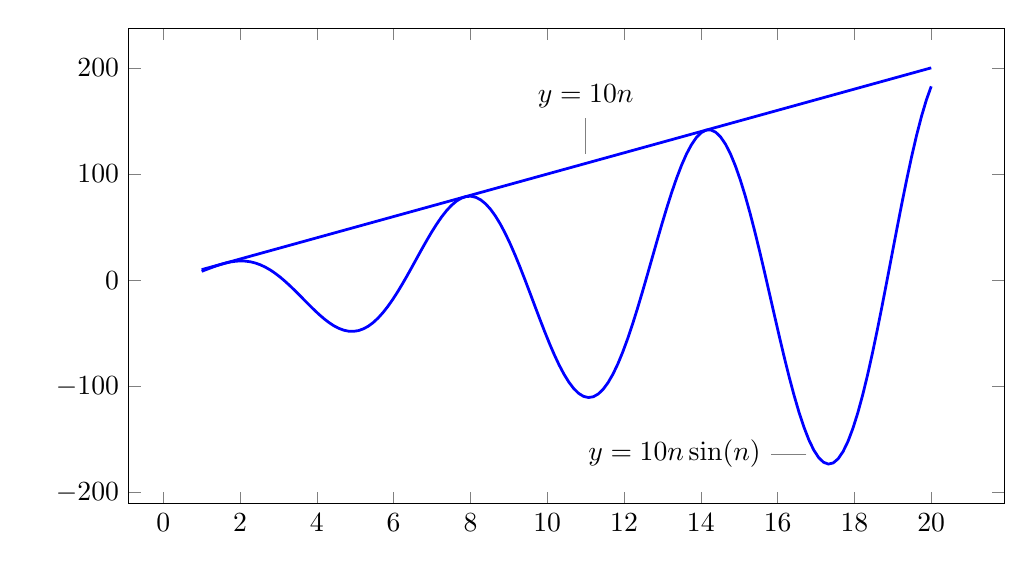
\begin{tikzpicture}[line width=1]
\begin{axis}[width=5in, height=3in,
             scatter/classes={a={mark=*,draw=black}},
             xlabel={\mbox{}},
             xlabel style={name=xlabel}, 
             ylabel={\mbox{}}, 
             legend style={
                at={(xlabel.south)},
                yshift=-1ex,
                anchor=north,
                legend cell align=left,
                },
        ]
]
\addplot[draw=blue, line width=1] coordinates {(1.0,10.0)
(10.5,105.0)
(20.0,200.0)
(20.0,200.0)};\node[pin=above:{$y=10   n$}] at (axis cs:11,110) {};\addplot[draw=blue, line width=1] coordinates {(1.0,8.4147)
(1.1275,10.1854)
(1.255,11.9298)
(1.3826,13.5813)
(1.5101,15.0728)
(1.6376,16.3393)
(1.7651,17.3189)
(1.8926,17.9545)
(2.0201,18.1961)
(2.1477,18.0012)
(2.2752,17.3372)
(2.4027,16.1816)
(2.5302,14.5235)
(2.6577,12.364)
(2.7852,9.7167)
(2.9128,6.6075)
(3.0403,3.0753)
(3.1678,-0.8296)
(3.2953,-5.0453)
(3.4228,-9.4995)
(3.5503,-14.111)
(3.6779,-18.791)
(3.8054,-23.4447)
(3.9329,-27.9732)
(4.0604,-32.2753)
(4.1879,-36.2502)
(4.3154,-39.7988)
(4.443,-42.8266)
(4.5705,-45.2452)
(4.698,-46.975)
(4.8255,-47.9467)
(4.953,-48.1031)
(5.0805,-47.4012)
(5.2081,-45.8128)
(5.3356,-43.3262)
(5.4631,-39.9468)
(5.5906,-35.6975)
(5.7181,-30.6188)
(5.8456,-24.7691)
(5.9732,-18.2234)
(6.1007,-11.0729)
(6.2282,-3.4236)
(6.3557,4.6051)
(6.4832,12.8825)
(6.6107,21.2685)
(6.7383,29.6163)
(6.8658,37.7745)
(6.9933,45.5901)
(7.1208,52.9113)
(7.2483,59.5904)
(7.3758,65.4865)
(7.5034,70.4684)
(7.6309,74.4174)
(7.7584,77.2297)
(7.8859,78.8189)
(8.0134,79.1178)
(8.1409,78.0805)
(8.2685,75.6835)
(8.396,71.9269)
(8.5235,66.835)
(8.651,60.4565)
(8.7785,52.8643)
(8.906,44.1547)
(9.0336,34.4465)
(9.1611,23.8791)
(9.2886,12.6108)
(9.4161,0.8164)
(9.5436,-11.3156)
(9.6711,-23.5858)
(9.7987,-35.7876)
(9.9262,-47.7102)
(10.0537,-59.1425)
(10.1812,-69.8766)
(10.3087,-79.712)
(10.4362,-88.4586)
(10.5638,-95.9408)
(10.6913,-102.0009)
(10.8188,-106.5018)
(10.9463,-109.3303)
(11.0738,-110.3994)
(11.2013,-109.6504)
(11.3289,-107.0546)
(11.4564,-102.6143)
(11.5839,-96.3635)
(11.7114,-88.3679)
(11.8389,-78.7245)
(11.9664,-67.5605)
(12.094,-55.0317)
(12.2215,-41.3204)
(12.349,-26.633)
(12.4765,-11.1964)
(12.604,4.7451)
(12.7315,20.9336)
(12.8591,37.1021)
(12.9866,52.9786)
(13.1141,68.291)
(13.2416,82.7713)
(13.3691,96.1607)
(13.4966,108.2139)
(13.6242,118.7037)
(13.7517,127.4251)
(13.8792,134.1992)
(14.0067,138.8769)
(14.1342,141.3417)
(14.2617,141.5122)
(14.3893,139.3445)
(14.5168,134.8331)
(14.6443,128.012)
(14.7718,118.9548)
(14.8993,107.7735)
(15.0268,94.6183)
(15.1544,79.6746)
(15.2819,63.1613)
(15.4094,45.3269)
(15.5369,26.4466)
(15.6644,6.8172)
(15.7919,-13.247)
(15.9195,-33.4192)
(16.047,-53.3658)
(16.1745,-72.7517)
(16.302,-91.2459)
(16.4295,-108.5272)
(16.557,-124.2897)
(16.6846,-138.2481)
(16.8121,-150.1432)
(16.9396,-159.7461)
(17.0671,-166.8629)
(17.1946,-171.3382)
(17.3221,-173.0585)
(17.4497,-171.9545)
(17.5772,-168.003)
(17.7047,-161.2281)
(17.8322,-151.7011)
(17.9597,-139.5401)
(18.0872,-124.9091)
(18.2148,-108.0152)
(18.3423,-89.1061)
(18.4698,-68.4666)
(18.5973,-46.4141)
(18.7248,-23.2938)
(18.8523,0.5266)
(18.9799,24.6627)
(19.1074,48.7199)
(19.2349,72.2996)
(19.3624,95.0058)
(19.4899,116.4519)
(19.6174,136.267)
(19.745,154.1027)
(19.8725,169.6388)
(20.0,182.5891)
(20.0,182.5891)};\node[pin=left:{$y=10   n   \sin(n)$}] at (axis cs:17,-163.43757361952467) {};
\end{axis}\end{tikzpicture}\end{center}


AHA!!!

This means that $3g(n) = 3n^2$ will beat $10n \sin n$ for large values of $n$.

Altogether, this means that the growth of 
\[
f(n) = 3n^2 + 5 + 10 n \sin (n)
\]
is roughly $3g(n) = 3n^2$
and therefore a higher multiple of $g(n) = n^2$ will beat
$f(n) = 3n^2 + 5 + 10 n \sin (n)$ for large values of $n$.

Here's the plot of $3g(n) = 3n^2$ and $f(n)$ for $0 \leq n \leq 10$:
%-*-latex-*-

\begin{center}
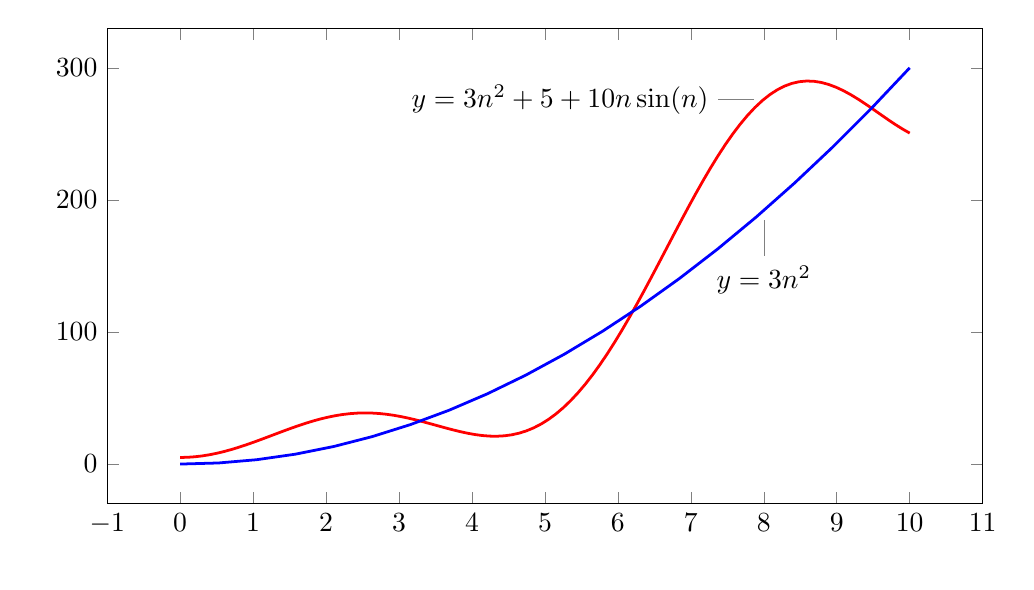
\begin{tikzpicture}[line width=1]
\begin{axis}[width=5in, height=3in,
             scatter/classes={a={mark=*,draw=black}},
             xlabel={\mbox{}},
             xlabel style={name=xlabel}, 
             ylabel={\mbox{}}, 
             legend style={
                at={(xlabel.south)},
                yshift=-1ex,
                anchor=north,
                legend cell align=left,
                },
        ]
]
\addplot[draw=red, line width=1] coordinates {(0.0,5.0)
(0.101,5.1325)
(0.202,5.5278)
(0.303,6.1798)
(0.404,7.0782)
(0.5051,8.2089)
(0.6061,9.5543)
(0.7071,11.093)
(0.8081,12.8011)
(0.9091,14.6516)
(1.0101,16.6153)
(1.1111,18.6614)
(1.2121,20.7576)
(1.3131,22.8708)
(1.4141,24.9676)
(1.5152,27.0151)
(1.6162,28.9809)
(1.7172,30.8341)
(1.8182,32.5456)
(1.9192,34.0888)
(2.0202,35.4397)
(2.1212,36.5779)
(2.2222,37.4864)
(2.3232,38.1524)
(2.4242,38.5676)
(2.5253,38.728)
(2.6263,38.6346)
(2.7273,38.2932)
(2.8283,37.7146)
(2.9293,36.9145)
(3.0303,35.9137)
(3.1313,34.7372)
(3.2323,33.4151)
(3.3333,31.9811)
(3.4343,30.4731)
(3.5354,28.9323)
(3.6364,27.4029)
(3.7374,25.9314)
(3.8384,24.5664)
(3.9394,23.3574)
(4.0404,22.3549)
(4.1414,21.6091)
(4.2424,21.1697)
(4.3434,21.0848)
(4.4444,21.4007)
(4.5455,22.1608)
(4.6465,23.4052)
(4.7475,25.17)
(4.8485,27.4869)
(4.9495,30.3823)
(5.0505,33.8773)
(5.1515,37.9868)
(5.2525,42.7194)
(5.3535,48.0772)
(5.4545,54.0555)
(5.5556,60.6425)
(5.6566,67.8195)
(5.7576,75.561)
(5.8586,83.8343)
(5.9596,92.6005)
(6.0606,101.8143)
(6.1616,111.4244)
(6.2626,121.374)
(6.3636,131.6017)
(6.4646,142.0415)
(6.5657,152.624)
(6.6667,163.2767)
(6.7677,173.9254)
(6.8687,184.4941)
(6.9697,194.907)
(7.0707,205.0882)
(7.1717,214.9636)
(7.2727,224.4613)
(7.3737,233.5124)
(7.4747,242.0521)
(7.5758,250.0206)
(7.6768,257.3637)
(7.7778,264.0335)
(7.8788,269.9895)
(7.9798,275.1987)
(8.0808,279.6366)
(8.1818,283.2871)
(8.2828,286.1436)
(8.3838,288.2087)
(8.4848,289.4945)
(8.5859,290.0229)
(8.6869,289.8253)
(8.7879,288.9424)
(8.8889,287.4242)
(8.9899,285.3294)
(9.0909,282.7249)
(9.1919,279.6854)
(9.2929,276.2927)
(9.3939,272.6348)
(9.4949,268.8049)
(9.596,264.9009)
(9.697,261.024)
(9.798,257.2779)
(9.899,253.7675)
(10.0,250.5979)
(10.0,250.5979)};\node[pin=left:{$y=3 n^2 + 5 + 10 n   \sin(n)$}] at (axis cs:8.0,276.14865972987053) {};\addplot[draw=blue, line width=1] coordinates {(0.0,0.0)
(0.5263,0.831)
(1.0526,3.3241)
(1.5789,7.4792)
(2.1053,13.2964)
(2.6316,20.7756)
(3.1579,29.9169)
(3.6842,40.7202)
(4.2105,53.1856)
(4.7368,67.313)
(5.2632,83.1025)
(5.7895,100.554)
(6.3158,119.6676)
(6.8421,140.4432)
(7.3684,162.8809)
(7.8947,186.9806)
(8.4211,212.7424)
(8.9474,240.1662)
(9.4737,269.2521)
(10.0,300.0)};\node[pin=below:{$y=3 n^2$}] at (axis cs:8.0,192.0) {};
\end{axis}\end{tikzpicture}\end{center}

It does seem like $f(n)$ winds itself around $3g(n) = 3n^2$.
To get a better feel for the pattern of things, I'm going 
to plot up to $n = 100$:
%-*-latex-*-

\begin{center}
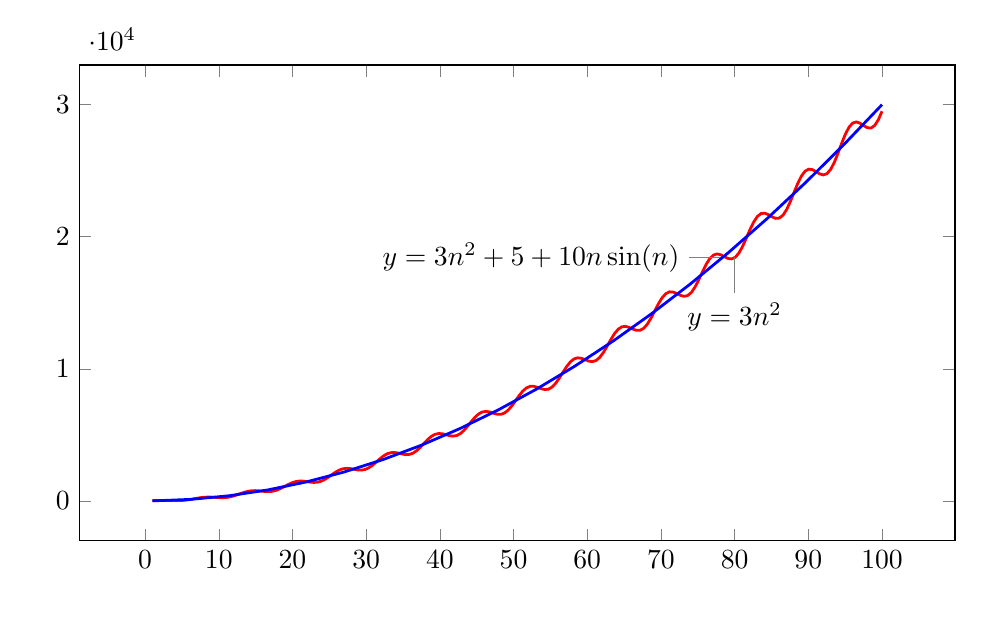
\begin{tikzpicture}[line width=1]
\begin{axis}[width=5in, height=3in,
             scatter/classes={a={mark=*,draw=black}},
             xlabel={\mbox{}},
             xlabel style={name=xlabel}, 
             ylabel={\mbox{}}, 
             legend style={
                at={(xlabel.south)},
                yshift=-1ex,
                anchor=north,
                legend cell align=left,
                },
        ]
]
\addplot[draw=red, line width=1] coordinates {(1.0,16.4147)
(1.4975,26.6621)
(1.995,35.1215)
(2.4925,38.7039)
(2.9899,36.3361)
(3.4874,29.6645)
(3.9849,22.8769)
(4.4824,21.6321)
(4.9799,31.3705)
(5.4774,55.4923)
(5.9749,93.9666)
(6.4724,142.8457)
(6.9698,194.9225)
(7.4673,241.4443)
(7.9648,274.4747)
(8.4623,289.2742)
(8.9598,286.0101)
(9.4573,270.2469)
(9.9548,251.9682)
(10.4523,243.2779)
(10.9497,255.3085)
(11.4472,295.1242)
(11.9447,363.4662)
(12.4422,454.0173)
(12.9397,554.5006)
(13.4372,649.4488)
(13.9347,724.025)
(14.4322,767.9493)
(14.9296,778.5013)
(15.4271,761.746)
(15.9246,731.5479)
(16.4221,706.4967)
(16.9196,705.4185)
(17.4171,742.5574)
(17.9146,823.6571)
(18.4121,944.0051)
(18.9095,1089.0504)
(19.407,1237.5717)
(19.9045,1366.7163)
(20.402,1457.7118)
(20.8995,1500.8269)
(21.397,1498.2766)
(21.8945,1464.2376)
(22.392,1421.8339)
(22.8894,1397.7235)
(23.3869,1415.5492)
(23.8844,1489.8643)
(24.3819,1622.0877)
(24.8794,1799.5948)
(25.3769,1998.3011)
(25.8744,2188.2285)
(26.3719,2340.7701)
(26.8693,2435.8938)
(27.3668,2467.4724)
(27.8643,2445.3342)
(28.3618,2393.3987)
(28.8593,2344.2251)
(29.3568,2331.2096)
(29.8543,2380.3023)
(30.3518,2503.2964)
(30.8492,2694.4187)
(31.3467,2931.1807)
(31.8442,3179.4187)
(32.3417,3401.3981)
(32.8392,3565.0632)
(33.3367,3652.1636)
(33.8342,3663.2011)
(34.3317,3617.8725)
(34.8291,3550.762)
(35.3266,3503.2167)
(35.8241,3513.3091)
(36.3216,3606.3257)
(36.8191,3788.1545)
(37.3166,4043.2913)
(37.8141,4338.0866)
(38.3116,4628.5682)
(38.809,4871.0266)
(39.3065,5032.8123)
(39.804,5100.6816)
(40.3015,5084.5614)
(40.799,5015.6861)
(41.2965,4939.4274)
(41.794,4904.4571)
(42.2915,4950.831)
(42.7889,5099.9112)
(43.2864,5348.6581)
(43.7839,5669.806)
(44.2814,6018.0129)
(44.7789,6340.6089)
(45.2764,6590.3925)
(45.7739,6737.3697)
(46.2714,6776.5154)
(46.7688,6729.5584)
(47.2663,6640.2187)
(47.7638,6563.931)
(48.2613,6554.4648)
(48.7588,6650.6736)
(49.2563,6866.6353)
(49.7538,7187.6822)
(50.2513,7573.4177)
(50.7487,7967.1189)
(51.2462,8309.3408)
(51.7437,8552.4595)
(52.2412,8672.596)
(52.7387,8675.9398)
(53.2362,8597.8082)
(53.7337,8494.5339)
(54.2312,8430.0395)
(54.7286,8460.2962)
(55.2261,8619.4466)
(55.7236,8911.0295)
(56.2211,9306.5547)
(56.7186,9751.9124)
(57.2161,10180.1819)
(57.7136,10527.8105)
(58.2111,10750.2515)
(58.7085,10833.2129)
(59.206,10796.6822)
(59.7035,10690.6153)
(60.201,10583.2043)
(60.6985,10544.4784)
(61.196,10629.1794)
(61.6935,10863.1008)
(62.191,11236.2951)
(62.6884,11704.9282)
(63.1859,12201.4661)
(63.6834,12650.8306)
(64.1809,12988.66)
(64.6784,13177.2337)
(65.1759,13215.1224)
(65.6734,13138.1009)
(66.1709,13010.9657)
(66.6683,12912.1223)
(67.1658,12914.6059)
(67.6633,13068.1313)
(68.1608,13386.5812)
(68.6583,13844.0787)
(69.1558,14380.7319)
(69.6533,14916.7858)
(70.1508,15371.8407)
(70.6482,15684.5052)
(71.1457,15827.6807)
(71.6432,15815.6748)
(72.1407,15701.287)
(72.6382,15563.4385)
(73.1357,15488.2414)
(73.6332,15548.0477)
(74.1307,15783.5745)
(74.6281,16193.5209)
(75.1256,16734.3177)
(75.6231,17330.2071)
(76.1206,17891.3264)
(76.6181,18335.4803)
(77.1156,18608.3257)
(77.6131,18697.0147)
(78.1106,18633.8725)
(78.608,18489.0841)
(79.1055,18354.0349)
(79.603,18319.2575)
(80.1005,18452.3074)
(80.598,18780.973)
(81.0955,19285.991)
(81.593,19905.1656)
(82.0905,20548.0268)
(82.5879,21117.5758)
(83.0854,21533.8905)
(83.5829,21753.8483)
(84.0804,21782.0982)
(84.5779,21670.4992)
(85.0754,21506.0221)
(85.5729,21389.9335)
(86.0704,21413.244)
(86.5678,21634.3717)
(87.0653,22064.5037)
(87.5628,22664.3183)
(88.0603,23353.0016)
(88.5578,24027.4953)
(89.0553,24587.3955)
(89.5528,24959.485)
(90.0503,25115.9058)
(90.5477,25081.465)
(91.0452,24928.1672)
(91.5427,24758.1678)
(92.0402,24679.1804)
(92.5377,24778.2575)
(93.0352,25100.3277)
(93.5327,25636.7788)
(94.0302,26326.9825)
(94.5276,27072.5271)
(95.0251,27760.8204)
(95.5226,28292.4034)
(96.0201,28605.3481)
(96.5176,28690.7555)
(97.0151,28595.4793)
(97.5126,28411.2771)
(98.0101,28252.8963)
(98.5075,28230.327)
(99.005,28421.9306)
(99.5025,28855.0098)
(100.0,29498.6344)
(100.0,29498.6344)};\node[pin=left:{$y=3 n^2 + 5 + 10 n   \sin(n)$}] at (axis cs:80.0,18409.8890768613) {};\addplot[draw=blue, line width=1] coordinates {(1.0,3.0)
(6.2105,115.7119)
(11.4211,391.3213)
(16.6316,829.8283)
(21.8421,1431.2327)
(27.0526,2195.5346)
(32.2632,3122.7341)
(37.4737,4212.831)
(42.6842,5465.8255)
(47.8947,6881.7175)
(53.1053,8460.5069)
(58.3158,10202.1939)
(63.5263,12106.7784)
(68.7368,14174.2604)
(73.9474,16404.6399)
(79.1579,18797.9169)
(84.3684,21354.0914)
(89.5789,24073.1634)
(94.7895,26955.133)
(100.0,30000.0)};\node[pin=below:{$y=3 n^2$}] at (axis cs:80.0,19200.0) {};
\end{axis}\end{tikzpicture}\end{center}

and then up to $n = 500$:
\input{definition_of_big_O_17.tex}

GRRREAT!!!

I see that 
$f(n) = 3n^2 + 5 + 10 n \sin (n)$
follows $3g(n)$ very tightly.
So to beat $f(n)$, let me try $4g(n) = 4n^2$
(... well ... I'm sure $(3.5)g(n)$ works too ... but I'll stick to $4g(n)$):
\input{definition_of_big_O_18.tex}

To see roughly when $4g(n) = 4n^2$ beats 
$f(n) = 3n^2 + 5 + 10n  \sin n$, I zoom in and plot 
the graphs for $0 \leq n \leq 30$:
%-*-latex-*-

\begin{center}
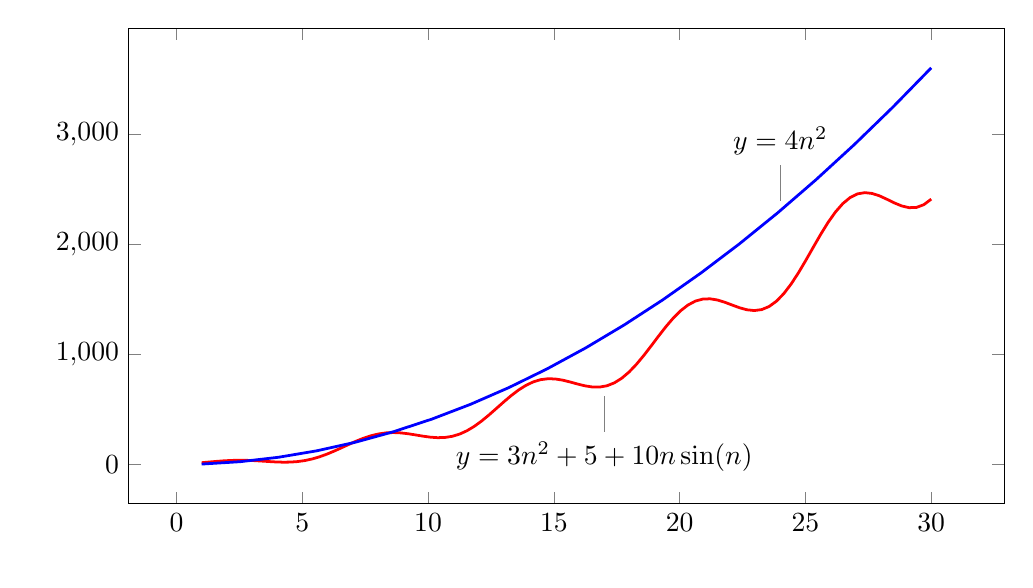
\begin{tikzpicture}[line width=1]
\begin{axis}[width=5in, height=3in,
             scatter/classes={a={mark=*,draw=black}},
             xlabel={\mbox{}},
             xlabel style={name=xlabel}, 
             ylabel={\mbox{}}, 
             legend style={
                at={(xlabel.south)},
                yshift=-1ex,
                anchor=north,
                legend cell align=left,
                },
        ]
]
\addplot[draw=red, line width=1] coordinates {(1.0,16.4147)
(1.2929,22.4484)
(1.5859,28.4016)
(1.8788,33.4933)
(2.1717,37.0617)
(2.4646,38.6624)
(2.7576,38.1439)
(3.0505,35.6915)
(3.3434,31.8329)
(3.6364,27.4029)
(3.9293,23.4698)
(4.2222,21.2307)
(4.5152,21.8837)
(4.8081,26.4921)
(5.101,35.8545)
(5.3939,50.3946)
(5.6869,70.0841)
(5.9798,94.409)
(6.2727,122.3853)
(6.5657,152.624)
(6.8586,183.443)
(7.1515,213.0165)
(7.4444,239.5475)
(7.7374,261.4491)
(8.0303,277.5153)
(8.3232,287.0641)
(8.6162,290.0382)
(8.9091,287.0493)
(9.202,279.3606)
(9.4949,268.8049)
(9.7879,257.6437)
(10.0808,248.3776)
(10.3737,243.5245)
(10.6667,245.3845)
(10.9596,255.8132)
(11.2525,276.027)
(11.5455,306.4575)
(11.8384,346.6732)
(12.1313,395.3773)
(12.4242,450.4864)
(12.7172,509.2844)
(13.0101,568.6421)
(13.303,625.2839)
(13.596,676.0796)
(13.8889,718.3338)
(14.1818,750.0487)
(14.4747,770.1327)
(14.7677,778.5354)
(15.0606,776.2931)
(15.3535,765.4782)
(15.6465,749.0519)
(15.9394,730.6326)
(16.2323,714.1964)
(16.5253,703.7343)
(16.8182,702.8971)
(17.1111,714.6583)
(17.404,741.0255)
(17.697,782.8302)
(17.9899,839.6146)
(18.2828,909.6296)
(18.5758,989.9493)
(18.8687,1076.6916)
(19.1616,1165.3326)
(19.4545,1251.0864)
(19.7475,1329.3198)
(20.0404,1395.9654)
(20.3333,1447.8973)
(20.6263,1483.2335)
(20.9192,1501.5372)
(21.2121,1503.896)
(21.5051,1492.8688)
(21.798,1472.3013)
(22.0909,1447.0233)
(22.3838,1422.4513)
(22.6768,1404.1289)
(22.9697,1397.2441)
(23.2626,1406.1662)
(23.5556,1434.0418)
(23.8485,1482.4895)
(24.1414,1551.4195)
(24.4343,1639.0007)
(24.7273,1741.7775)
(25.0202,1854.9334)
(25.3131,1972.679)
(25.6061,2088.7345)
(25.899,2196.8663)
(26.1919,2291.4312)
(26.4848,2367.8821)
(26.7778,2423.1883)
(27.0707,2456.1332)
(27.3636,2467.4598)
(27.6566,2459.8485)
(27.9495,2437.7253)
(28.2424,2406.9141)
(28.5354,2374.1592)
(28.8283,2346.5586)
(29.1212,2330.9541)
(29.4141,2333.3321)
(29.7071,2358.2861)
(30.0,2408.5905)};\node[pin=below:{$y=3 n^2+5+10 n \sin(n)$}] at (axis cs:17,708.5624263804754) {};\addplot[draw=blue, line width=1] coordinates {(1.0,4.0)
(2.5263,25.5291)
(4.0526,65.6953)
(5.5789,124.4986)
(7.1053,201.9391)
(8.6316,298.0166)
(10.1579,412.7313)
(11.6842,546.0831)
(13.2105,698.072)
(14.7368,868.6981)
(16.2632,1057.9612)
(17.7895,1265.8615)
(19.3158,1492.3989)
(20.8421,1737.5734)
(22.3684,2001.385)
(23.8947,2283.8338)
(25.4211,2584.9197)
(26.9474,2904.6427)
(28.4737,3243.0028)
(30.0,3600.0)};\node[pin=above:{$y=4 n^2$}] at (axis cs:24.0,2304.0) {};
\end{axis}\end{tikzpicture}\end{center}

It looks like $4g(n)$ definitely beats $f(n)$ for \textit{all} $n$
such that $n \geq 10$.
(Actually I can zoom in further and see if \lq\lq $n \geq 9$''
works as well ... but I'll just use \lq\lq $n \geq 10$''.)

That's it!!!

We can now say that 
\[
3n^2 + 5 + 10 n \sin (n) \leq 4n^2 \text{ for $n \geq 10$}
\]
Therefore, if I choose $C = 4$ and $N = 10$, I can say that
\[
|f(n)| \leq C |g(n)| \text{ for $n \geq N$}
\]
(Don't forget that $f(n)$ is positive for $n \geq 0$.)
This means that I can now say
\[
f(n) = O(g(n))
\]

Now we are ready for the formal definition of big-O:

\begin{defn}
Let $f(n)$ and $g(n)$ be functions.
We write 
\[
f(n) = O(g(n)) \tinysidebar{$O$}
\]
and say that 
\lq\lq $f(n)$ is \defone{big-O} of $g(n)$"
if we can find a $C$ and an $N$ such that 
for all $n \geq N$, we have
\[
|f(n)| \leq C|g(n)|
\]
\end{defn}

So now I'm ready to give a proper presentation of my solution to
the previous problem:

\newpage
\begin{eg}
Show graphically that if 
$f(n) = 3n^2 + 5 + 10 n \sin (n)$
and $g(n) = n^2$, then
\[
f(n) = O(g(n))
\]
\end{eg}

\textit{Solution.}
Let $N = 10$ and $C = 4$.
From the following graphs:
%-*-latex-*-

\begin{center}
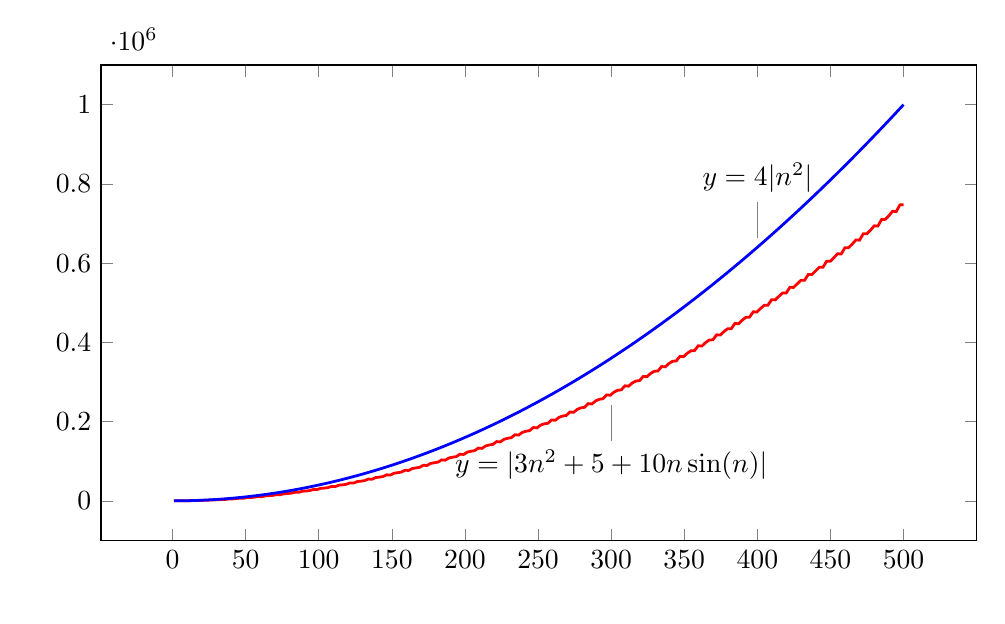
\begin{tikzpicture}[line width=1]
\begin{axis}[width=5in, height=3in,
             scatter/classes={a={mark=*,draw=black}},
             xlabel={\mbox{}},
             xlabel style={name=xlabel}, 
             ylabel={\mbox{}}, 
             legend style={
                at={(xlabel.south)},
                yshift=-1ex,
                anchor=north,
                legend cell align=left,
                },
        ]
]
\addplot[draw=red, line width=1] coordinates {(1.0,16.4147)
(3.5075,29.3574)
(6.0151,97.6089)
(8.5226,289.7793)
(11.0302,259.7571)
(13.5377,666.5782)
(16.0452,724.2533)
(18.5528,983.3568)
(21.0603,1504.5391)
(23.5678,1435.6548)
(26.0754,2255.7543)
(28.5829,2369.1408)
(31.0905,2805.4344)
(33.598,3666.6159)
(36.1055,3554.8658)
(38.6131,4783.6926)
(41.1206,4964.113)
(43.6281,5563.9419)
(46.1357,6775.7553)
(48.6432,6617.6994)
(51.1508,8250.1501)
(53.6583,8509.2517)
(56.1658,9258.9908)
(58.6734,10831.6961)
(61.1809,10624.4644)
(63.6884,12654.891)
(66.196,13004.6274)
(68.7035,13890.7034)
(71.2111,15834.1708)
(73.7186,15575.4686)
(76.2261,17997.6876)
(78.7337,18450.2989)
(81.2412,19459.2131)
(83.7487,21782.9061)
(86.2563,21471.0185)
(88.7638,24278.3198)
(91.2714,24846.3135)
(93.7789,25964.6638)
(96.2864,28677.6232)
(98.794,28311.4188)
(101.3015,31496.5763)
(103.809,32192.7066)
(106.3166,33407.2098)
(108.8241,36518.0382)
(111.3317,36096.9721)
(113.8392,39652.2543)
(116.3467,40489.502)
(118.8543,41787.0158)
(121.3618,45303.8624)
(123.8693,44827.9782)
(126.3769,48745.1598)
(128.8844,49736.7115)
(131.392,51104.2565)
(133.8995,55034.8027)
(136.407,54504.7341)
(138.9146,58775.1085)
(141.4221,59934.3354)
(143.9296,61359.1164)
(146.4372,65710.5621)
(148.9447,65127.5331)
(151.4523,69741.9251)
(153.9598,71082.3617)
(156.4673,72551.7897)
(158.9749,77330.8399)
(161.4824,76696.6648)
(163.9899,81645.4444)
(166.4975,83180.7668)
(169.005,84682.4797)
(171.5126,89895.3324)
(174.0201,89212.4146)
(176.5276,94485.5111)
(179.0352,96229.5153)
(181.5427,97751.3991)
(184.0503,103403.7331)
(186.5578,102675.0631)
(189.0653,108261.9801)
(191.5729,110228.5597)
(194.0804,111758.7692)
(196.5879,117855.7332)
(199.0955,117084.886)
(201.603,122974.7167)
(204.1106,125177.841)
(206.6181,126704.8197)
(209.1256,133251.0218)
(211.6332,132442.1535)
(214.1407,138623.597)
(216.6482,141077.2883)
(219.1558,142589.7887)
(221.6633,149589.2866)
(224.1709,148747.1301)
(226.6784,155208.5078)
(229.1859,157926.8192)
(231.6935,159413.9223)
(234.201,166870.2144)
(236.7085,166000.074)
(239.2161,172729.3471)
(241.7236,175726.3396)
(244.2312,177177.474)
(246.7387,185093.491)
(249.2462,184201.2368)
(251.7538,191186.0239)
(254.2613,194475.744)
(256.7688,195880.7045)
(259.2764,204258.8024)
(261.7839,203350.8635)
(264.2915,210578.4586)
(266.799,214174.9154)
(269.3065,215523.8817)
(271.8141,224365.8343)
(274.3216,223449.1915)
(276.8291,230906.5831)
(279.3367,234823.7259)
(281.8442,236107.2799)
(284.3518,245414.2735)
(286.8593,244496.4508)
(289.3668,252170.3409)
(291.8744,256422.0363)
(294.3819,257631.1796)
(296.8894,267403.8074)
(299.397,266492.8634)
(301.9045,274369.6873)
(304.4121,278969.6964)
(306.9196,280095.8674)
(309.4271,290334.1253)
(311.9347,289438.6432)
(314.4422,297504.5891)
(316.9497,302466.5454)
(319.4573,303501.6351)
(321.9648,314204.9182)
(324.4724,313333.9953)
(326.9799,321575.0253)
(329.4874,326912.412)
(331.995,327848.7799)
(334.5025,339015.8794)
(337.0101,338179.1161)
(339.5176,346580.9868)
(342.0251,352307.1142)
(344.5327,353137.6034)
(347.0402,364766.7049)
(349.5477,363974.1928)
(352.0553,372522.4764)
(354.5628,378650.4602)
(357.0704,379368.412)
(359.5779,391457.0941)
(362.0854,390719.403)
(364.593,399399.509)
(367.1005,405942.2481)
(369.608,406541.5156)
(372.1156,419086.7498)
(374.6231,418414.9149)
(377.1307,427212.1116)
(379.6382,434182.2664)
(382.1457,434657.228)
(384.6533,447655.3788)
(387.1608,447060.8863)
(389.6683,455960.3232)
(392.1759,463370.2938)
(394.6834,463715.8658)
(397.191,477162.6924)
(399.6985,476657.4651)
(402.206,485644.1949)
(404.7136,493506.1003)
(407.2211,493717.7487)
(409.7286,507608.4066)
(412.2362,507204.7887)
(414.7437,516263.79)
(417.2513,524589.4467)
(419.7588,524663.1984)
(422.2663,538992.2426)
(424.7739,538702.9835)
(427.2814,547819.1836)
(429.7889,556620.0851)
(432.2965,556552.5387)
(434.804,571313.9275)
(437.3116,571152.1653)
(439.8191,580310.4628)
(442.3266,589597.7595)
(444.8342,589386.0947)
(447.3417,604573.194)
(449.8492,604552.4388)
(452.3568,613737.7267)
(454.8643,623522.2056)
(457.3719,623164.1926)
(459.8794,638769.7813)
(462.3869,638903.8971)
(464.8945,648101.0861)
(467.402,658393.1515)
(469.9095,657887.1592)
(472.4171,673903.4355)
(474.9246,674206.6221)
(477.4322,683400.6637)
(479.9397,694210.318)
(482.4472,693555.3216)
(484.9548,709973.9097)
(487.4623,710460.6839)
(489.9698,719636.5937)
(492.4774,730973.4187)
(494.9849,730169.0065)
(497.4925,746980.9644)
(500.0,747666.141)
(500.0,747666.141)};\node[pin=below:{$y=|3n^2 + 5 + 10n \sin(n)|$}] at (axis cs:300,267005.7324802966) {};\addplot[draw=blue, line width=1] coordinates {(1.0,4.0)
(6.0404,145.9459)
(11.0808,491.1372)
(16.1212,1039.5739)
(21.1616,1791.256)
(26.202,2746.1835)
(31.2424,3904.3563)
(36.2828,5265.7745)
(41.3232,6830.4381)
(46.3636,8598.3471)
(51.404,10569.5015)
(56.4444,12743.9012)
(61.4848,15121.5464)
(66.5253,17702.4369)
(71.5657,20486.5728)
(76.6061,23473.9541)
(81.6465,26664.5808)
(86.6869,30058.4528)
(91.7273,33655.5702)
(96.7677,37455.9331)
(101.8081,41459.5413)
(106.8485,45666.3949)
(111.8889,50076.4938)
(116.9293,54689.8382)
(121.9697,59506.4279)
(127.0101,64526.263)
(132.0505,69749.3435)
(137.0909,75175.6694)
(142.1313,80805.2407)
(147.1717,86638.0573)
(152.2121,92674.1194)
(157.2525,98913.4268)
(162.2929,105355.9796)
(167.3333,112001.7778)
(172.3737,118850.8213)
(177.4141,125903.1103)
(182.4545,133158.6446)
(187.4949,140617.4243)
(192.5354,148279.4494)
(197.5758,156144.7199)
(202.6162,164213.2358)
(207.6566,172484.997)
(212.697,180960.0037)
(217.7374,189638.2557)
(222.7778,198519.7531)
(227.8182,207604.4959)
(232.8586,216892.484)
(237.899,226383.7176)
(242.9394,236078.1965)
(247.9798,245975.9208)
(253.0202,256076.8905)
(258.0606,266381.1056)
(263.101,276888.5661)
(268.1414,287599.2719)
(273.1818,298513.2231)
(278.2222,309630.4198)
(283.2626,320950.8617)
(288.303,332474.5491)
(293.3434,344201.4819)
(298.3838,356131.66)
(303.4242,368265.0836)
(308.4646,380601.7525)
(313.5051,393141.6668)
(318.5455,405884.8264)
(323.5859,418831.2315)
(328.6263,431980.882)
(333.6667,445333.7778)
(338.7071,458889.919)
(343.7475,472649.3056)
(348.7879,486611.9376)
(353.8283,500777.8149)
(358.8687,515146.9377)
(363.9091,529719.3058)
(368.9495,544494.9193)
(373.9899,559473.7782)
(379.0303,574655.8825)
(384.0707,590041.2321)
(389.1111,605629.8272)
(394.1515,621421.6676)
(399.1919,637416.7534)
(404.2323,653615.0846)
(409.2727,670016.6612)
(414.3131,686621.4831)
(419.3535,703429.5505)
(424.3939,720440.8632)
(429.4343,737655.4213)
(434.4747,755073.2248)
(439.5152,772694.2736)
(444.5556,790518.5679)
(449.596,808546.1075)
(454.6364,826776.8926)
(459.6768,845210.923)
(464.7172,863848.1988)
(469.7576,882688.7199)
(474.798,901732.4865)
(479.8384,920979.4984)
(484.8788,940429.7557)
(489.9192,960083.2584)
(494.9596,979940.0065)
(500.0,1000000.0)};\node[pin=above:{$y=4|n^2|$}] at (axis cs:400.0,640000.0) {};
\end{axis}\end{tikzpicture}\end{center}

\input{definition_of_big_O_22.tex}
we see that, for $n \geq N$, we have:
\[
|3n^2 + 5 + 10n \sin(n)| \leq C |n^2|
\]
i.e.,
\[
|f(n)| \leq C|g(n)|
\]
Hence $f(n) = O(g(n)$.
\qed

Remember that technically speaking you cannot prove a mathematical
fact like $f(n) = O(g(n))$ using graphs
because a graph cannot possibly show you that a multiple of $|g(n)|$
beats $|f(n)|$ for \textit{all} sufficiently large $n$.
A graph can only show you the graphs up to some \textit{finite} $n$.
How would you know that the graph 
of $|f(n)|$ won't suddenly shoot up and overtake $4|g(n)|$ at 
$n = 1000000000000$?
Later, I'll show you how to prove big-O statements without a shadow of doubt.

Now, let me give you another example.
Suppose I change my $f(n)$ to \textit{this}:
\[
f(n) = -3n^2 + 5 - 10 n \sin (n)
\]
then when I plot
$|-3n^2 + 5 - 10 n \sin (n)|$ 
and $4|n^2|$ for $0 \leq n \leq 5$,
I get
%-*-latex-*-

\begin{center}
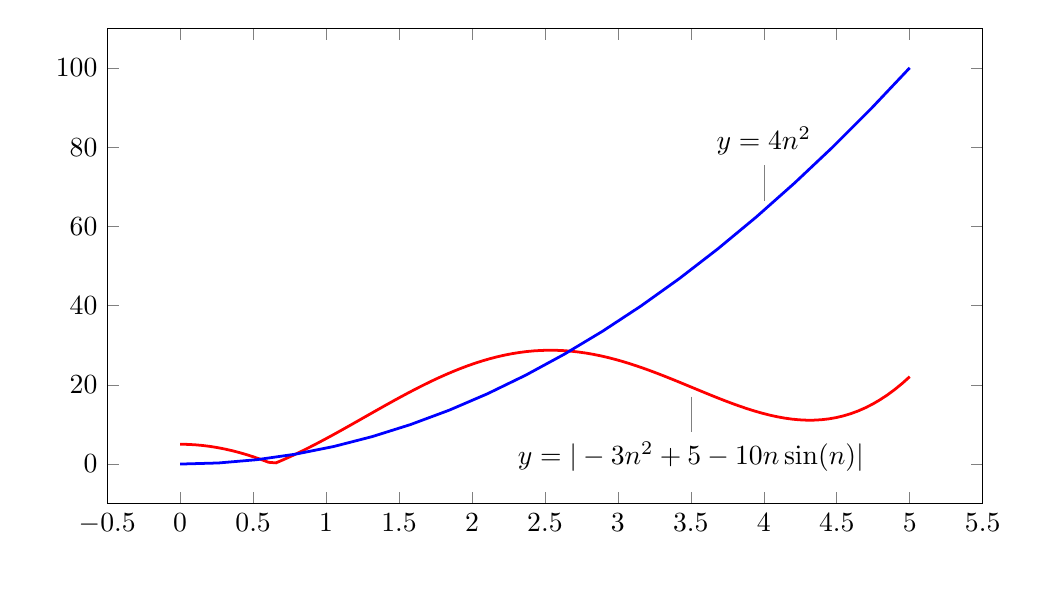
\begin{tikzpicture}[line width=1]
\begin{axis}[width=5in, height=3in,
             scatter/classes={a={mark=*,draw=black}},
             xlabel={\mbox{}},
             xlabel style={name=xlabel}, 
             ylabel={\mbox{}}, 
             legend style={
                at={(xlabel.south)},
                yshift=-1ex,
                anchor=north,
                legend cell align=left,
                },
        ]
]
\addplot[draw=red, line width=1] coordinates {(0.0,5.0)
(0.0505,4.9669)
(0.101,4.8675)
(0.1515,4.7024)
(0.202,4.4722)
(0.2525,4.1778)
(0.303,3.8202)
(0.3535,3.401)
(0.404,2.9218)
(0.4545,2.3845)
(0.5051,1.7911)
(0.5556,1.144)
(0.6061,0.4457)
(0.6566,0.3009)
(0.7071,1.093)
(0.7576,1.9275)
(0.8081,2.8011)
(0.8586,3.7103)
(0.9091,4.6516)
(0.9596,5.6212)
(1.0101,6.6153)
(1.0606,7.6301)
(1.1111,8.6614)
(1.1616,9.7053)
(1.2121,10.7576)
(1.2626,11.8141)
(1.3131,12.8708)
(1.3636,13.9233)
(1.4141,14.9676)
(1.4646,15.9996)
(1.5152,17.0151)
(1.5657,18.0102)
(1.6162,18.9809)
(1.6667,19.9235)
(1.7172,20.8341)
(1.7677,21.7093)
(1.8182,22.5456)
(1.8687,23.3398)
(1.9192,24.0888)
(1.9697,24.7897)
(2.0202,25.4397)
(2.0707,26.0365)
(2.1212,26.5779)
(2.1717,27.0617)
(2.2222,27.4864)
(2.2727,27.8503)
(2.3232,28.1524)
(2.3737,28.3917)
(2.4242,28.5676)
(2.4747,28.6797)
(2.5253,28.728)
(2.5758,28.7128)
(2.6263,28.6346)
(2.6768,28.4943)
(2.7273,28.2932)
(2.7778,28.0326)
(2.8283,27.7146)
(2.8788,27.3411)
(2.9293,26.9145)
(2.9798,26.4377)
(3.0303,25.9137)
(3.0808,25.3456)
(3.1313,24.7372)
(3.1818,24.0923)
(3.2323,23.4151)
(3.2828,22.7098)
(3.3333,21.9811)
(3.3838,21.2338)
(3.4343,20.4731)
(3.4848,19.7041)
(3.5354,18.9323)
(3.5859,18.1633)
(3.6364,17.4029)
(3.6869,16.6569)
(3.7374,15.9314)
(3.7879,15.2325)
(3.8384,14.5664)
(3.8889,13.9392)
(3.9394,13.3574)
(3.9899,12.8272)
(4.0404,12.3549)
(4.0909,11.9468)
(4.1414,11.6091)
(4.1919,11.3481)
(4.2424,11.1697)
(4.2929,11.08)
(4.3434,11.0848)
(4.3939,11.1899)
(4.4444,11.4007)
(4.4949,11.7226)
(4.5455,12.1608)
(4.596,12.7201)
(4.6465,13.4052)
(4.697,14.2205)
(4.7475,15.17)
(4.798,16.2577)
(4.8485,17.4869)
(4.899,18.8608)
(4.9495,20.3823)
(5.0,22.0538)
(5.0,22.0538)};\node[pin=below:{$y=|-3n^2+5-10n \sin(n)|$}] at (axis cs:3.5,19.472587030863306) {};\addplot[draw=blue, line width=1] coordinates {(0.0,0.0)
(0.2632,0.277)
(0.5263,1.108)
(0.7895,2.4931)
(1.0526,4.4321)
(1.3158,6.9252)
(1.5789,9.9723)
(1.8421,13.5734)
(2.1053,17.7285)
(2.3684,22.4377)
(2.6316,27.7008)
(2.8947,33.518)
(3.1579,39.8892)
(3.4211,46.8144)
(3.6842,54.2936)
(3.9474,62.3269)
(4.2105,70.9141)
(4.4737,80.0554)
(4.7368,89.7507)
(5.0,100.0)};\node[pin=above:{$y=4 n^2$}] at (axis cs:4.0,64.0) {};
\end{axis}\end{tikzpicture}\end{center}

and then for $0 \leq n \leq 100$:
\input{definition_of_big_O_24.tex}
In this case $n^2$ still works, i.e., 
$-3n^2 + 5 - 10 n \sin (n) = O(n^2)$.
Also, it seems that $4n^2$ breaks away from 
$|-3n^2+5-10n \sin(n)|$ around $n = 20$.
So let's plot the graphs for $0 \leq n \leq 20$:
%-*-latex-*-

\begin{center}
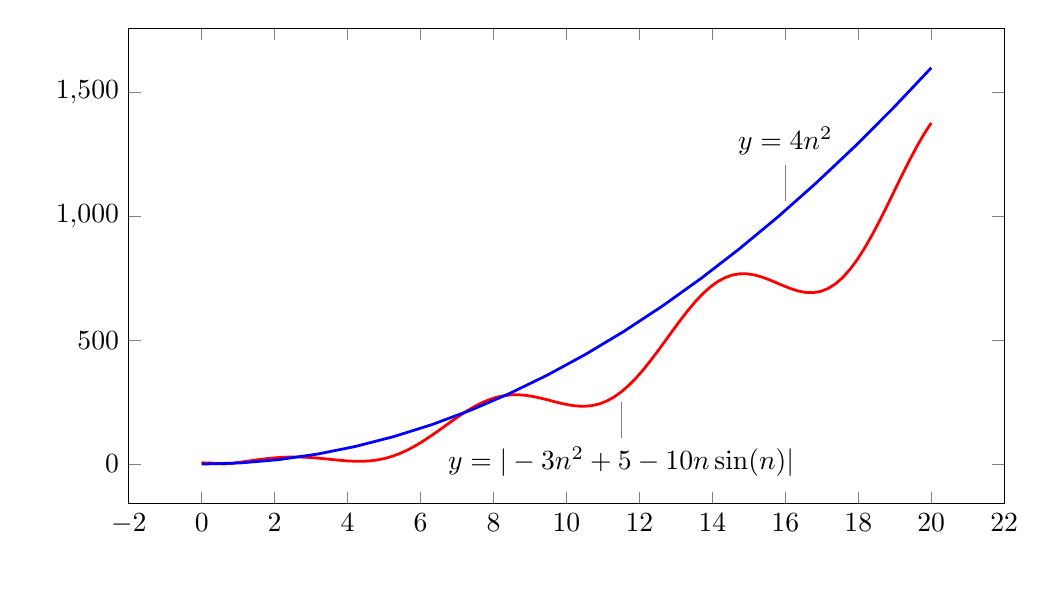
\begin{tikzpicture}[line width=1]
\begin{axis}[width=5in, height=3in,
             scatter/classes={a={mark=*,draw=black}},
             xlabel={\mbox{}},
             xlabel style={name=xlabel}, 
             ylabel={\mbox{}}, 
             legend style={
                at={(xlabel.south)},
                yshift=-1ex,
                anchor=north,
                legend cell align=left,
                },
        ]
]
\addplot[draw=red, line width=1] coordinates {(0.0,5.0)
(0.202,4.4722)
(0.404,2.9218)
(0.6061,0.4457)
(0.8081,2.8011)
(1.0101,6.6153)
(1.2121,10.7576)
(1.4141,14.9676)
(1.6162,18.9809)
(1.8182,22.5456)
(2.0202,25.4397)
(2.2222,27.4864)
(2.4242,28.5676)
(2.6263,28.6346)
(2.8283,27.7146)
(3.0303,25.9137)
(3.2323,23.4151)
(3.4343,20.4731)
(3.6364,17.4029)
(3.8384,14.5664)
(4.0404,12.3549)
(4.2424,11.1697)
(4.4444,11.4007)
(4.6465,13.4052)
(4.8485,17.4869)
(5.0505,23.8773)
(5.2525,32.7194)
(5.4545,44.0555)
(5.6566,57.8195)
(5.8586,73.8343)
(6.0606,91.8143)
(6.2626,111.374)
(6.4646,132.0415)
(6.6667,153.2767)
(6.8687,174.4941)
(7.0707,195.0882)
(7.2727,214.4613)
(7.4747,232.0521)
(7.6768,247.3637)
(7.8788,259.9895)
(8.0808,269.6366)
(8.2828,276.1436)
(8.4848,279.4945)
(8.6869,279.8253)
(8.8889,277.4242)
(9.0909,272.7249)
(9.2929,266.2927)
(9.4949,258.8049)
(9.697,251.024)
(9.899,243.7675)
(10.101,237.8732)
(10.303,234.1627)
(10.5051,233.4047)
(10.7071,236.2785)
(10.9091,243.3416)
(11.1111,255.0)
(11.3131,271.486)
(11.5152,292.8413)
(11.7172,318.9095)
(11.9192,349.3361)
(12.1212,383.5773)
(12.3232,420.918)
(12.5253,460.4972)
(12.7273,501.3406)
(12.9293,542.3998)
(13.1313,582.5949)
(13.3333,620.8602)
(13.5354,656.1907)
(13.7374,687.687)
(13.9394,714.5968)
(14.1414,736.3516)
(14.3434,752.5962)
(14.5455,763.2092)
(14.7475,768.3154)
(14.9495,768.2864)
(15.1515,763.7315)
(15.3535,755.4782)
(15.5556,744.5421)
(15.7576,732.0891)
(15.9596,719.389)
(16.1616,707.7649)
(16.3636,698.5379)
(16.5657,692.971)
(16.7677,692.2147)
(16.9697,697.2553)
(17.1717,708.8693)
(17.3737,727.5859)
(17.5758,753.659)
(17.7778,787.0499)
(17.9798,827.4227)
(18.1818,874.1517)
(18.3838,926.3413)
(18.5859,982.858)
(18.7879,1042.3727)
(18.9899,1103.4124)
(19.1919,1164.4193)
(19.3939,1223.8141)
(19.596,1280.062)
(19.798,1331.7381)
(20.0,1377.5891)
(20.0,1377.5891)};\node[pin=below:{$y=|-3n^2+5-10n \sin(n)|$}] at (axis cs:11.5,291.07299991083073) {};\addplot[draw=blue, line width=1] coordinates {(0.0,0.0)
(1.0526,4.4321)
(2.1053,17.7285)
(3.1579,39.8892)
(4.2105,70.9141)
(5.2632,110.8033)
(6.3158,159.5568)
(7.3684,217.1745)
(8.4211,283.6565)
(9.4737,359.0028)
(10.5263,443.2133)
(11.5789,536.2881)
(12.6316,638.2271)
(13.6842,749.0305)
(14.7368,868.6981)
(15.7895,997.2299)
(16.8421,1134.626)
(17.8947,1280.8864)
(18.9474,1436.0111)
(20.0,1600.0)};\node[pin=above:{$y=4 n^2$}] at (axis cs:16.0,1024.0) {};
\end{axis}\end{tikzpicture}\end{center}

Clearly for $n \geq 10$, $4|g(n)|$ beats $|f(n)|$.
So I'm going to pick $N = 10$.

Now I'm ready to present this ...

\newpage

\begin{eg}
Let $f(n) = -3n^2+5-10n \sin(n)$ and $g(n) = n^2$.
Show graphically that 
\[
f(n) = O(g(n))
\]
\end{eg}

\textit{Solution.}
From the following graphs:
\input{definition_of_big_O_26.tex}
%-*-latex-*-

\begin{center}
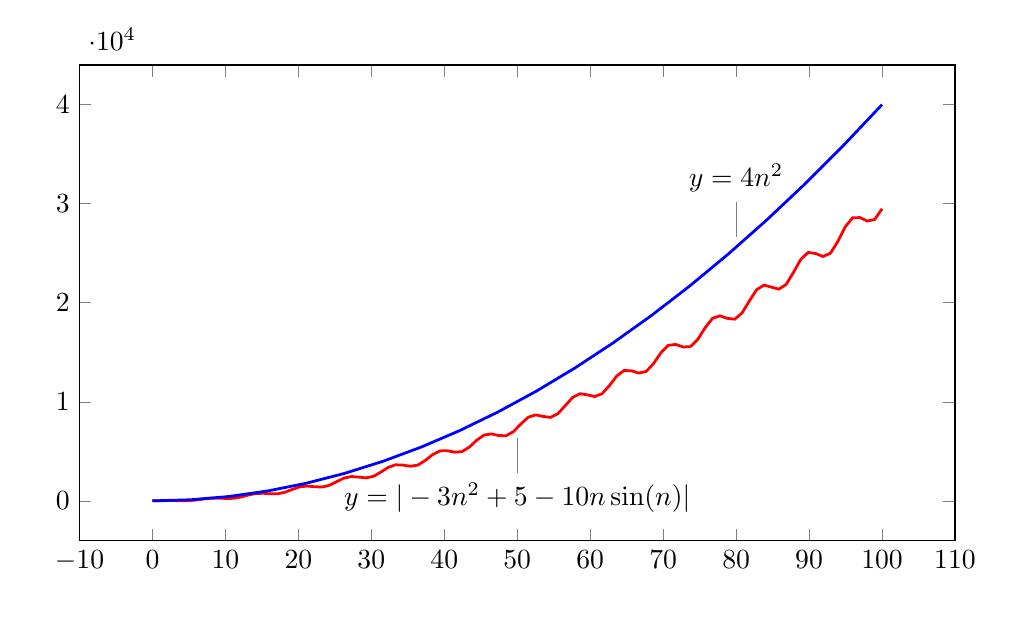
\begin{tikzpicture}[line width=1]
\begin{axis}[width=5in, height=3in,
             scatter/classes={a={mark=*,draw=black}},
             xlabel={\mbox{}},
             xlabel style={name=xlabel}, 
             ylabel={\mbox{}}, 
             legend style={
                at={(xlabel.south)},
                yshift=-1ex,
                anchor=north,
                legend cell align=left,
                },
        ]
]
\addplot[draw=red, line width=1] coordinates {(0.0,5.0)
(1.0101,6.6153)
(2.0202,25.4397)
(3.0303,25.9137)
(4.0404,12.3549)
(5.0505,23.8773)
(6.0606,91.8143)
(7.0707,195.0882)
(8.0808,269.6366)
(9.0909,272.7249)
(10.101,237.8732)
(11.1111,255.0)
(12.1212,383.5773)
(13.1313,582.5949)
(14.1414,736.3516)
(15.1515,763.7315)
(16.1616,707.7649)
(17.1717,708.8693)
(18.1818,874.1517)
(19.1919,1164.4193)
(20.202,1416.5891)
(21.2121,1493.896)
(22.2222,1425.5875)
(23.2323,1394.4064)
(24.2424,1569.656)
(25.2525,1938.2463)
(26.2626,2301.6861)
(27.2727,2456.1335)
(28.2828,2392.3527)
(29.2929,2319.8353)
(30.303,2478.008)
(31.3131,2904.4048)
(32.3232,3384.0318)
(33.3333,3641.8432)
(34.3434,3606.3782)
(35.3535,3491.9899)
(36.3636,3608.3278)
(37.3737,4065.9185)
(38.3838,4657.72)
(39.3939,5041.5605)
(40.404,5063.3358)
(41.4141,4915.7123)
(42.4242,4970.241)
(43.4343,5428.359)
(44.4444,6119.0909)
(45.4545,6645.6871)
(46.4646,6756.4949)
(47.4747,6593.3826)
(48.4848,6573.1284)
(49.4949,6999.509)
(50.5051,7767.1203)
(51.5152,8445.2496)
(52.5253,8677.1483)
(53.5354,8524.6161)
(54.5455,8425.3713)
(55.5556,8788.8539)
(56.5657,9603.6299)
(57.5758,10432.6353)
(58.5859,10815.1947)
(59.596,10706.1514)
(60.6061,10533.6472)
(61.6162,10806.9348)
(62.6263,11633.2978)
(63.6364,12602.2548)
(64.6465,13159.841)
(65.6566,13131.942)
(66.6667,12902.3213)
(67.6768,13064.6013)
(68.6869,13863.4655)
(69.697,14951.0841)
(70.7071,15700.3808)
(71.7172,15793.4493)
(72.7273,15532.9807)
(73.7374,15572.215)
(74.7475,16303.7479)
(75.7576,17479.0458)
(76.7677,18426.9974)
(77.7778,18680.1241)
(78.7879,18424.1447)
(79.798,18338.8533)
(80.8081,18965.4674)
(81.8182,20189.2011)
(82.8283,21331.5386)
(83.8384,21780.0485)
(84.8485,21571.1764)
(85.8586,21371.5687)
(86.8687,21860.9452)
(87.8788,23087.7309)
(88.8889,24408.2113)
(89.899,25080.7016)
(90.9091,24966.4088)
(91.9192,24674.7531)
(92.9293,25002.6904)
(93.9394,26183.7035)
(94.9495,27654.146)
(95.9596,28569.8024)
(96.9697,28599.4829)
(97.9798,28249.6545)
(98.9899,28402.5388)
(100.0,29488.6344)};\node[pin=below:{$y=|-3n^2+5-10n \sin(n)|$}] at (axis cs:50,7363.812573148036) {};\addplot[draw=blue, line width=1] coordinates {(0.0,0.0)
(5.2632,110.8033)
(10.5263,443.2133)
(15.7895,997.2299)
(21.0526,1772.8532)
(26.3158,2770.0831)
(31.5789,3988.9197)
(36.8421,5429.3629)
(42.1053,7091.4127)
(47.3684,8975.0693)
(52.6316,11080.3324)
(57.8947,13407.2022)
(63.1579,15955.6787)
(68.4211,18725.7618)
(73.6842,21717.4515)
(78.9474,24930.7479)
(84.2105,28365.651)
(89.4737,32022.1607)
(94.7368,35900.277)
(100.0,40000.0)};\node[pin=above:{$y=4 n^2$}] at (axis cs:80.0,25600.0) {};
\end{axis}\end{tikzpicture}\end{center}

we see that if we choose $C = 4$ and $N  = 20$, then for $n \geq N$,
we have
\[
|-3n^2+5-10n \sin(n)| \leq 4|n^2|
\]
i.e.,
\[
|f(n)| \leq C|g(n)|
\]
Hence $f(n) = O(g(n))$.
\qed

\newpage

It's not surprising that if 
\[
3n^2 + 5 + 10 n \sin (n) = O(n^2)
\]
then it is also true that 
\[
3n^2 + 5 + 10 n \sin (n) = O(n^3)
\]
since $n^3$ grows faster than $n^2$.
So there are many possible functions to \lq\lq control''
$3n^2 + 5 + 10n \sin(n)$ from above.
Also, if
\[
|3n^2 + 5 + 10 n \sin (n)| \leq C|n^2|
\]
then of course if you replace $C$ by a large value, say $C + 1423$,
then of course
\[
|3n^2 + 5 + 10 n \sin (n)| \leq (C + 1423)|n^2|
\]
is still true for $n \geq N$.
Furthermore, this is also true if you replace $N$ by a larger value
such as $N + 15313$.
Therefore the choice of $C$ and $N$ is not unique.


Here's another example.

Let
\[
f(n) = \frac{2n^5}{1 + n} \sin \frac{1000}{n} - 100
\]
Let's find some function $g(n)$ of the form $n^0, n^1, n^2, n^3$ or ...
such that $f(n) = O(g(n))$.
Let's have a few plots to get a feel for the function.

Here's the plot of $f(n)$ for $0 \leq n \leq 10$:
%-*-latex-*-

\begin{center}
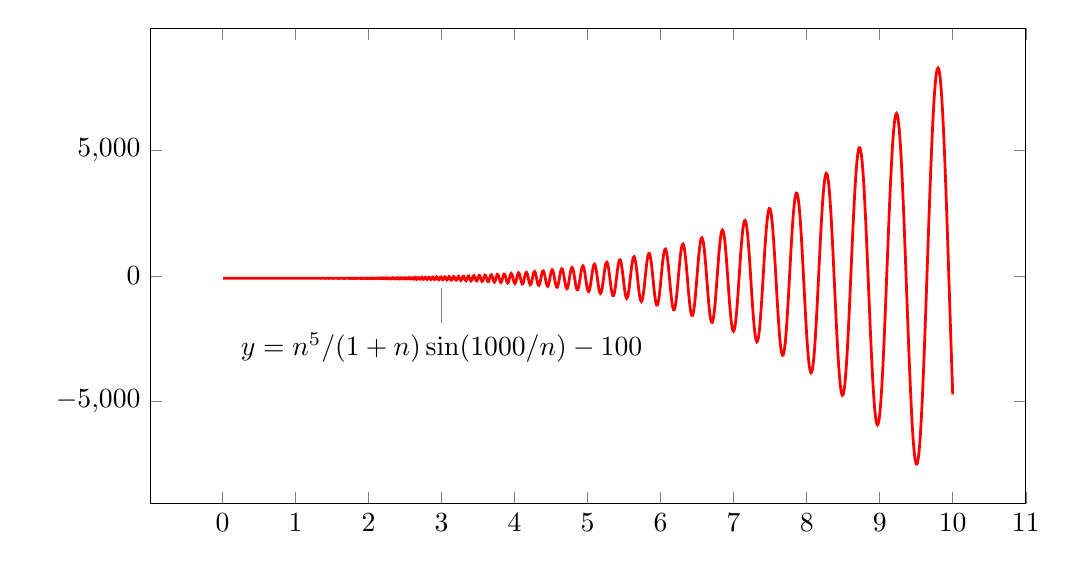
\begin{tikzpicture}[line width=1]
\begin{axis}[width=5in, height=3in,
             scatter/classes={a={mark=*,draw=black}},
             xlabel={\mbox{}},
             xlabel style={name=xlabel}, 
             ylabel={\mbox{}}, 
             legend style={
                at={(xlabel.south)},
                yshift=-1ex,
                anchor=north,
                legend cell align=left,
                },
        ]
]
\addplot[draw=red, line width=1] coordinates {(0.01,-100.0)
(0.02,-100.0)
(0.03,-100.0)
(0.04,-100.0)
(0.0501,-100.0)
(0.0601,-100.0)
(0.0701,-100.0)
(0.0801,-100.0)
(0.0901,-100.0)
(0.1001,-100.0)
(0.1101,-100.0)
(0.1201,-100.0)
(0.1301,-100.0)
(0.1401,-100.0)
(0.1502,-100.0)
(0.1602,-100.0001)
(0.1702,-99.9999)
(0.1802,-99.9999)
(0.1902,-100.0002)
(0.2002,-100.0)
(0.2102,-99.9998)
(0.2202,-100.0004)
(0.2302,-99.9995)
(0.2402,-99.9999)
(0.2503,-100.0001)
(0.2603,-100.0001)
(0.2703,-100.0008)
(0.2803,-100.0011)
(0.2903,-99.9984)
(0.3003,-100.0002)
(0.3103,-100.0014)
(0.3203,-100.0019)
(0.3303,-100.0028)
(0.3403,-100.0026)
(0.3504,-99.9961)
(0.3604,-100.0037)
(0.3704,-100.005)
(0.3804,-99.9969)
(0.3904,-100.0059)
(0.4004,-99.9995)
(0.4104,-100.0079)
(0.4204,-100.0035)
(0.4304,-100.0103)
(0.4404,-99.9909)
(0.4505,-99.9886)
(0.4605,-100.0111)
(0.4705,-99.9848)
(0.4805,-99.9827)
(0.4905,-99.9978)
(0.5005,-100.0011)
(0.5105,-100.0229)
(0.5205,-100.0251)
(0.5305,-100.0014)
(0.5405,-99.9884)
(0.5506,-99.9837)
(0.5606,-100.0169)
(0.5706,-100.0142)
(0.5806,-99.9695)
(0.5906,-99.9956)
(0.6006,-100.0022)
(0.6106,-100.0424)
(0.6206,-99.9807)
(0.6306,-99.9565)
(0.6406,-99.9723)
(0.6507,-100.0447)
(0.6607,-100.0435)
(0.6707,-99.924)
(0.6807,-100.0793)
(0.6907,-99.9597)
(0.7007,-99.9247)
(0.7107,-100.0404)
(0.7207,-100.0999)
(0.7307,-100.1139)
(0.7407,-100.0991)
(0.7508,-100.0048)
(0.7608,-99.861)
(0.7708,-99.9885)
(0.7808,-100.1372)
(0.7908,-99.8277)
(0.8008,-100.1828)
(0.8108,-99.8129)
(0.8208,-100.1231)
(0.8308,-100.0811)
(0.8408,-99.7759)
(0.8509,-99.92)
(0.8609,-100.1753)
(0.8709,-100.2677)
(0.8809,-100.2529)
(0.8909,-100.2367)
(0.9009,-100.2657)
(0.9109,-100.3226)
(0.9209,-100.3106)
(0.9309,-100.083)
(0.9409,-99.7005)
(0.951,-99.6993)
(0.961,-100.2872)
(0.971,-100.2272)
(0.981,-99.5422)
(0.991,-100.2866)
(1.001,-100.0133)
(1.011,-99.7515)
(1.021,-100.3803)
(1.031,-99.5693)
(1.041,-100.4085)
(1.0511,-99.7145)
(1.0611,-100.0163)
(1.0711,-100.3797)
(1.0811,-99.3044)
(1.0911,-100.5463)
(1.1011,-100.1992)
(1.1111,-99.1996)
(1.1211,-100.205)
(1.1311,-100.8332)
(1.1411,-99.8306)
(1.1512,-99.0613)
(1.1612,-99.6102)
(1.1712,-100.6279)
(1.1812,-101.0529)
(1.1912,-100.6972)
(1.2012,-99.9749)
(1.2112,-99.316)
(1.2212,-98.9084)
(1.2312,-98.7374)
(1.2412,-98.7051)
(1.2513,-98.7135)
(1.2613,-98.6972)
(1.2713,-98.6291)
(1.2813,-98.5218)
(1.2913,-98.4333)
(1.3013,-98.4725)
(1.3113,-98.7831)
(1.3213,-99.4779)
(1.3313,-100.5081)
(1.3413,-101.5244)
(1.3514,-101.8936)
(1.3614,-101.075)
(1.3714,-99.3033)
(1.3814,-97.9406)
(1.3914,-98.5626)
(1.4014,-100.9381)
(1.4114,-102.315)
(1.4214,-100.4658)
(1.4314,-97.7263)
(1.4414,-98.6852)
(1.4515,-102.1477)
(1.4615,-101.5752)
(1.4715,-97.6395)
(1.4815,-98.7688)
(1.4915,-102.8627)
(1.5015,-100.0538)
(1.5115,-96.9846)
(1.5215,-101.9416)
(1.5315,-101.6252)
(1.5415,-96.5773)
(1.5516,-101.6573)
(1.5616,-101.7388)
(1.5716,-96.3051)
(1.5816,-102.7984)
(1.5916,-100.0656)
(1.6016,-97.0887)
(1.6116,-104.1607)
(1.6216,-96.6112)
(1.6316,-101.1842)
(1.6416,-101.4311)
(1.6517,-96.4487)
(1.6617,-104.6718)
(1.6717,-95.2906)
(1.6817,-103.8715)
(1.6917,-97.5104)
(1.7017,-100.8896)
(1.7117,-100.6794)
(1.7217,-97.9346)
(1.7317,-103.2022)
(1.7417,-95.9153)
(1.7518,-104.7427)
(1.7618,-94.7808)
(1.7718,-105.5553)
(1.7818,-94.2201)
(1.7918,-105.9045)
(1.8018,-94.0809)
(1.8118,-105.792)
(1.8218,-94.5292)
(1.8318,-104.8871)
(1.8418,-96.0333)
(1.8519,-102.6468)
(1.8619,-99.0985)
(1.8719,-98.7737)
(1.8819,-103.5905)
(1.8919,-94.0828)
(1.9019,-107.8044)
(1.9119,-91.2332)
(1.9219,-108.3379)
(1.9319,-93.7686)
(1.9419,-102.5287)
(1.952,-102.1706)
(1.962,-93.268)
(1.972,-109.6948)
(1.982,-90.2638)
(1.992,-106.3004)
(2.002,-99.8583)
(2.012,-93.4337)
(2.022,-110.8471)
(2.032,-89.7559)
(2.042,-104.3574)
(2.0521,-104.3135)
(2.0621,-88.9055)
(2.0721,-111.573)
(2.0821,-95.3475)
(2.0921,-94.1491)
(2.1021,-112.8617)
(2.1121,-89.2482)
(2.1221,-100.1721)
(2.1321,-111.165)
(2.1421,-86.2686)
(2.1522,-104.3922)
(2.1622,-109.4646)
(2.1722,-84.875)
(2.1822,-106.2788)
(2.1922,-109.388)
(2.2022,-83.9634)
(2.2122,-105.7045)
(2.2222,-111.4917)
(2.2322,-83.6447)
(2.2422,-102.1623)
(2.2523,-115.3265)
(2.2623,-85.449)
(2.2723,-95.1491)
(2.2823,-118.7818)
(2.2923,-91.8666)
(2.3023,-85.839)
(2.3123,-117.5281)
(2.3223,-104.1439)
(2.3323,-79.3426)
(2.3423,-106.9063)
(2.3524,-117.9793)
(2.3624,-84.1523)
(2.3724,-88.4371)
(2.3824,-121.3509)
(2.3924,-103.6763)
(2.4024,-76.4811)
(2.4124,-103.9897)
(2.4224,-123.2152)
(2.4324,-89.4886)
(2.4424,-78.4954)
(2.4525,-115.5909)
(2.4625,-119.3337)
(2.4725,-80.691)
(2.4825,-82.5854)
(2.4925,-121.8984)
(2.5025,-116.2298)
(2.5125,-76.4175)
(2.5225,-83.9191)
(2.5325,-124.476)
(2.5425,-117.1332)
(2.5526,-75.4692)
(2.5626,-80.5715)
(2.5726,-123.5181)
(2.5826,-122.8565)
(2.5926,-78.9562)
(2.6026,-72.9149)
(2.6126,-116.6155)
(2.6226,-131.4681)
(2.6326,-90.2189)
(2.6426,-65.0309)
(2.6527,-100.3591)
(2.6627,-136.1652)
(2.6727,-111.2488)
(2.6827,-66.5771)
(2.6927,-76.269)
(2.7027,-125.3258)
(2.7127,-134.6763)
(2.7227,-88.6249)
(2.7327,-59.2491)
(2.7427,-92.829)
(2.7528,-138.4801)
(2.7628,-126.6767)
(2.7728,-74.2894)
(2.7828,-58.7105)
(2.7928,-103.4479)
(2.8028,-144.4373)
(2.8128,-122.7875)
(2.8228,-68.2253)
(2.8328,-56.6493)
(2.8428,-104.7187)
(2.8529,-147.6561)
(2.8629,-127.4459)
(2.8729,-70.1016)
(2.8829,-50.5877)
(2.8929,-94.8274)
(2.9029,-146.8884)
(2.9129,-140.805)
(2.9229,-83.3933)
(2.9329,-45.056)
(2.9429,-72.9663)
(2.953,-134.2823)
(2.963,-156.2209)
(2.973,-112.3702)
(2.983,-52.9834)
(2.993,-46.2618)
(3.003,-100.5382)
(3.013,-155.5643)
(3.023,-150.2114)
(3.033,-89.593)
(3.043,-38.7764)
(3.0531,-52.357)
(3.0631,-116.7428)
(3.0731,-165.158)
(3.0831,-147.3267)
(3.0931,-80.6805)
(3.1031,-31.9667)
(3.1131,-50.034)
(3.1231,-117.8389)
(3.1331,-169.8365)
(3.1431,-155.726)
(3.1532,-88.1914)
(3.1632,-30.2144)
(3.1732,-35.861)
(3.1832,-100.6502)
(3.1932,-166.3266)
(3.2032,-173.8673)
(3.2132,-115.9348)
(3.2232,-42.7)
(3.2332,-17.5855)
(3.2432,-62.665)
(3.2533,-140.4329)
(3.2633,-185.9931)
(3.2733,-161.2194)
(3.2833,-85.6927)
(3.2933,-20.1203)
(3.3033,-17.1679)
(3.3133,-79.8156)
(3.3233,-159.6335)
(3.3333,-194.9436)
(3.3433,-158.2441)
(3.3534,-76.6251)
(3.3634,-10.7952)
(3.3734,-9.6847)
(3.3834,-74.739)
(3.3934,-159.4614)
(3.4034,-203.329)
(3.4134,-174.8611)
(3.4234,-93.3229)
(3.4334,-14.7371)
(3.4434,6.9867)
(3.4535,-43.415)
(3.4635,-132.8045)
(3.4735,-202.2344)
(3.4835,-205.9565)
(3.4935,-140.9551)
(3.5035,-48.3478)
(3.5135,13.2874)
(3.5235,4.9412)
(3.5335,-68.8218)
(3.5435,-163.2172)
(3.5536,-220.9944)
(3.5636,-207.0542)
(3.5736,-129.0734)
(3.5836,-32.4443)
(3.5936,26.6619)
(3.6036,13.8306)
(3.6136,-64.2283)
(3.6236,-163.9863)
(3.6336,-229.8827)
(3.6436,-225.1968)
(3.6537,-151.9038)
(3.6637,-49.1185)
(3.6737,28.3288)
(3.6837,39.1637)
(3.6937,-22.8438)
(3.7037,-126.0836)
(3.7137,-217.8269)
(3.7237,-251.3134)
(3.7337,-209.2176)
(3.7437,-111.9136)
(3.7538,-6.9539)
(3.7638,54.4841)
(3.7738,42.3722)
(3.7838,-38.071)
(3.7938,-149.2919)
(3.8038,-239.4049)
(3.8138,-266.4424)
(3.8238,-217.5042)
(3.8338,-114.2599)
(3.8438,-2.7648)
(3.8539,67.3644)
(3.8639,64.8811)
(3.8739,-9.6737)
(3.8839,-124.6003)
(3.8939,-230.9981)
(3.9039,-283.706)
(3.9139,-260.2091)
(3.9239,-169.7138)
(3.9339,-48.9672)
(3.9439,53.0556)
(3.954,95.06)
(3.964,59.8343)
(3.974,-39.239)
(3.984,-163.8028)
(3.994,-265.7136)
(4.004,-305.6579)
(4.014,-268.0019)
(4.024,-166.3913)
(4.034,-38.2997)
(4.044,69.1136)
(4.0541,116.3856)
(4.0641,85.9629)
(4.0741,-11.7625)
(4.0841,-142.4905)
(4.0941,-260.3889)
(4.1041,-324.2276)
(4.1141,-311.5746)
(4.1241,-226.2484)
(4.1341,-96.7038)
(4.1441,33.8274)
(4.1542,121.9046)
(4.1642,138.2051)
(4.1742,76.9314)
(4.1842,-42.5969)
(4.1942,-182.4395)
(4.2042,-298.3106)
(4.2142,-353.5915)
(4.2242,-330.6551)
(4.2342,-236.0829)
(4.2442,-98.3609)
(4.2543,41.0217)
(4.2643,140.194)
(4.2743,169.3743)
(4.2843,119.5117)
(4.2943,4.685)
(4.3043,-142.2508)
(4.3143,-279.3187)
(4.3243,-367.4679)
(4.3343,-381.547)
(4.3443,-317.1653)
(4.3544,-191.6625)
(4.3644,-39.0954)
(4.3744,99.2193)
(4.3844,185.9235)
(4.3944,197.5483)
(4.4044,130.5626)
(4.4144,2.0652)
(4.4244,-154.9025)
(4.4344,-300.0578)
(4.4444,-396.2519)
(4.4545,-418.8378)
(4.4645,-361.7112)
(4.4745,-238.6124)
(4.4845,-79.5078)
(4.4945,76.923)
(4.5045,192.7602)
(4.5145,239.9437)
(4.5245,206.8396)
(4.5345,100.7975)
(4.5445,-53.7886)
(4.5546,-221.3355)
(4.5646,-363.3827)
(4.5746,-447.3955)
(4.5846,-454.0514)
(4.5946,-381.4195)
(4.6046,-245.1909)
(4.6146,-75.0207)
(4.6246,92.1093)
(4.6346,219.9834)
(4.6446,280.9209)
(4.6547,261.5729)
(4.6647,165.5791)
(4.6747,12.6129)
(4.6847,-165.8837)
(4.6947,-333.3053)
(4.7047,-455.4141)
(4.7147,-507.2435)
(4.7247,-478.0062)
(4.7347,-373.0822)
(4.7447,-212.7758)
(4.7548,-28.1733)
(4.7648,145.0128)
(4.7748,273.3724)
(4.7848,332.1524)
(4.7948,309.8484)
(4.8048,210.2191)
(4.8148,51.4161)
(4.8248,-137.5289)
(4.8348,-322.1453)
(4.8448,-468.85)
(4.8549,-550.9924)
(4.8649,-553.5444)
(4.8749,-475.6387)
(4.8849,-330.5656)
(4.8949,-143.2986)
(4.9049,53.9576)
(4.9149,227.3763)
(4.9249,347.2903)
(4.9349,393.1595)
(4.9449,356.9155)
(4.955,244.1682)
(4.965,73.1315)
(4.975,-128.4941)
(4.985,-328.1222)
(4.995,-493.5829)
(5.005,-598.2596)
(5.015,-625.2496)
(5.025,-569.9188)
(5.035,-440.4934)
(5.045,-256.6479)
(5.0551,-46.3603)
(5.0651,158.4425)
(5.0751,326.7551)
(5.0851,433.1376)
(5.0951,461.4444)
(5.1051,407.1111)
(5.1151,277.7012)
(5.1251,91.677)
(5.1351,-124.3808)
(5.1451,-339.6664)
(5.1552,-523.5725)
(5.1652,-650.0059)
(5.1752,-700.992)
(5.1852,-669.0871)
(5.1952,-558.2938)
(5.2052,-383.3936)
(5.2152,-167.8279)
(5.2252,59.5512)
(5.2352,268.3947)
(5.2452,430.9003)
(5.2553,525.4468)
(5.2653,539.3571)
(5.2753,470.4494)
(5.2853,327.2099)
(5.2953,127.5982)
(5.3053,-103.3283)
(5.3153,-336.642)
(5.3253,-543.1995)
(5.3353,-697.2584)
(5.3453,-779.6115)
(5.3554,-779.8667)
(5.3654,-697.6176)
(5.3754,-542.3905)
(5.3854,-332.4048)
(5.3954,-92.3232)
(5.4054,149.718)
(5.4154,365.4332)
(5.4254,529.6712)
(5.4354,623.2809)
(5.4454,635.2404)
(5.4555,563.8268)
(5.4655,416.7162)
(5.4755,210.0311)
(5.4855,-33.536)
(5.4955,-287.2897)
(5.5055,-523.495)
(5.5155,-716.4016)
(5.5255,-845.003)
(5.5355,-895.2392)
(5.5455,-861.4236)
(5.5556,-746.7601)
(5.5656,-562.9189)
(5.5756,-328.7378)
(5.5856,-68.2046)
(5.5956,192.0561)
(5.6056,425.5216)
(5.6156,608.4537)
(5.6256,722.2564)
(5.6356,755.2801)
(5.6456,703.9079)
(5.6557,572.8322)
(5.6657,374.516)
(5.6757,127.9074)
(5.6857,-143.4476)
(5.6957,-413.702)
(5.7057,-657.1849)
(5.7157,-850.8205)
(5.7257,-976.2641)
(5.7357,-1021.5625)
(5.7457,-982.1965)
(5.7558,-861.4232)
(5.7658,-669.9049)
(5.7758,-424.6732)
(5.7858,-147.5376)
(5.7958,136.9059)
(5.8058,403.4815)
(5.8158,628.6542)
(5.8258,792.5717)
(5.8358,880.7525)
(5.8458,885.2833)
(5.8559,805.4341)
(5.8659,647.6526)
(5.8759,424.9509)
(5.8859,155.7521)
(5.8959,-137.6967)
(5.9059,-431.2014)
(5.9159,-700.6293)
(5.9259,-923.8786)
(5.9359,-1082.6529)
(5.9459,-1163.8995)
(5.956,-1160.805)
(5.966,-1073.2786)
(5.976,-907.8968)
(5.986,-677.3248)
(5.996,-399.2733)
(6.006,-95.0801)
(6.016,211.9644)
(6.026,498.4143)
(6.036,742.4492)
(6.046,925.5042)
(6.0561,1033.6299)
(6.0661,1058.4883)
(6.0761,997.9168)
(6.0861,856.0307)
(6.0961,642.8651)
(6.1061,373.5935)
(6.1161,67.3878)
(6.1261,-253.9891)
(6.1361,-567.7541)
(6.1461,-851.7221)
(6.1562,-1085.8563)
(6.1662,-1253.6457)
(6.1762,-1343.2166)
(6.1862,-1348.1071)
(6.1962,-1267.6603)
(6.2062,-1107.0161)
(6.2162,-876.7122)
(6.2262,-591.9288)
(6.2362,-271.4353)
(6.2462,63.6846)
(6.2563,391.4404)
(6.2663,690.3803)
(6.2763,940.9798)
(6.2863,1126.8847)
(6.2963,1235.931)
(6.3063,1260.883)
(6.3163,1199.8477)
(6.3263,1056.3463)
(6.3363,839.0459)
(6.3463,561.1756)
(6.3564,239.6689)
(6.3664,-105.9074)
(6.3764,-454.5703)
(6.3864,-785.2036)
(6.3964,-1077.8314)
(6.4064,-1314.8029)
(6.4164,-1481.822)
(6.4264,-1568.7624)
(6.4364,-1570.2264)
(6.4464,-1485.8181)
(6.4565,-1320.1229)
(6.4665,-1082.3998)
(6.4765,-786.0103)
(6.4865,-447.6213)
(6.4965,-86.2338)
(6.5065,277.9063)
(6.5165,624.4512)
(6.5265,934.0821)
(6.5365,1189.5674)
(6.5465,1376.6908)
(6.5566,1485.0002)
(6.5666,1508.3429)
(6.5766,1445.1595)
(6.5866,1298.5285)
(6.5966,1075.9625)
(6.6066,788.9728)
(6.6166,452.4296)
(6.6266,83.756)
(6.6366,-297.9995)
(6.6466,-673.1604)
(6.6567,-1022.4384)
(6.6667,-1327.9144)
(6.6767,-1573.9362)
(6.6867,-1747.8884)
(6.6967,-1840.7998)
(6.7067,-1847.7589)
(6.7167,-1768.1241)
(6.7267,-1605.5182)
(6.7367,-1367.616)
(6.7467,-1065.7367)
(6.7568,-714.2655)
(6.7668,-329.9361)
(6.7768,68.9885)
(6.7868,463.5974)
(6.7968,835.2301)
(6.8068,1166.3514)
(6.8168,1441.3606)
(6.8268,1647.3)
(6.8368,1774.4306)
(6.8468,1816.6526)
(6.8569,1771.7533)
(6.8669,1641.4757)
(6.8769,1431.407)
(6.8869,1150.6966)
(6.8969,811.619)
(6.9069,429.0041)
(6.9169,19.5631)
(6.9269,-398.8589)
(6.9369,-808.0693)
(6.9469,-1190.3187)
(6.957,-1529.0612)
(6.967,-1809.653)
(6.977,-2019.9598)
(6.987,-2150.8501)
(6.997,-2196.5552)
(7.007,-2154.8827)
(7.017,-2027.2793)
(7.027,-1818.741)
(7.037,-1537.5795)
(7.047,-1195.0553)
(7.0571,-804.8959)
(7.0671,-382.7213)
(7.0771,54.5992)
(7.0871,489.6318)
(7.0971,905.0753)
(7.1071,1284.444)
(7.1171,1612.7094)
(7.1271,1876.8756)
(7.1371,2066.4685)
(7.1471,2173.9204)
(7.1572,2194.8377)
(7.1672,2128.1438)
(7.1772,1976.0935)
(7.1872,1744.1613)
(7.1972,1440.8107)
(7.2072,1077.1534)
(7.2172,666.516)
(7.2272,223.9298)
(7.2372,-234.4355)
(7.2472,-691.8714)
(7.2573,-1131.743)
(7.2673,-1538.0891)
(7.2773,-1896.1916)
(7.2873,-2193.0916)
(7.2973,-2418.0368)
(7.3073,-2562.8448)
(7.3173,-2622.1705)
(7.3273,-2593.6712)
(7.3373,-2478.0649)
(7.3473,-2279.0816)
(7.3574,-2003.3115)
(7.3674,-1659.9574)
(7.3774,-1260.5008)
(7.3874,-818.296)
(7.3974,-348.1055)
(7.4074,134.4053)
(7.4174,613.197)
(7.4274,1072.3903)
(7.4374,1496.789)
(7.4474,1872.3719)
(7.4575,2186.7417)
(7.4675,2429.5146)
(7.4775,2592.6398)
(7.4875,2670.6399)
(7.4975,2660.7665)
(7.5075,2563.0662)
(7.5175,2380.3582)
(7.5275,2118.1249)
(7.5375,1784.3197)
(7.5475,1389.1018)
(7.5576,944.5052)
(7.5676,464.0542)
(7.5776,-37.6612)
(7.5876,-545.4374)
(7.5976,-1043.9219)
(7.6076,-1518.0771)
(7.6176,-1953.6277)
(7.6276,-2337.4809)
(7.6376,-2658.1053)
(7.6476,-2905.8591)
(7.6577,-3073.2591)
(7.6677,-3155.1827)
(7.6777,-3148.999)
(7.6877,-3054.6262)
(7.6977,-2874.5152)
(7.7077,-2613.5606)
(7.7177,-2278.9431)
(7.7277,-1879.9103)
(7.7377,-1427.5004)
(7.7477,-934.2203)
(7.7578,-413.6868)
(7.7678,119.7591)
(7.7778,651.4529)
(7.7878,1166.8108)
(7.7978,1651.7267)
(7.8078,2092.9521)
(7.8178,2478.4471)
(7.8278,2797.6951)
(7.8378,3041.9724)
(7.8478,3204.5675)
(7.8579,3280.9439)
(7.8679,3268.8431)
(7.8779,3168.328)
(7.8879,2981.7636)
(7.8979,2713.7394)
(7.9079,2370.9351)
(7.9179,1961.9334)
(7.9279,1496.9877)
(7.9379,987.7496)
(7.9479,446.9637)
(7.958,-111.86)
(7.968,-674.79)
(7.978,-1227.8233)
(7.988,-1757.2324)
(7.998,-2249.9018)
(8.008,-2693.6456)
(8.018,-3077.4974)
(8.028,-3391.9688)
(8.038,-3629.2672)
(8.048,-3783.4716)
(8.0581,-3850.6607)
(8.0681,-3828.9918)
(8.0781,-3718.7302)
(8.0881,-3522.2273)
(8.0981,-3243.8511)
(8.1081,-2889.8701)
(8.1181,-2468.2937)
(8.1281,-1988.6756)
(8.1381,-1461.8826)
(8.1481,-899.8372)
(8.1582,-315.2384)
(8.1682,278.7313)
(8.1782,868.7064)
(8.1882,1441.4397)
(8.1982,1984.0972)
(8.2082,2484.5402)
(8.2182,2931.5888)
(8.2282,3315.2613)
(8.2382,3626.9842)
(8.2482,3859.7693)
(8.2583,4008.3543)
(8.2683,4069.3038)
(8.2783,4041.071)
(8.2883,3924.0174)
(8.2983,3720.3917)
(8.3083,3434.2696)
(8.3183,3071.4548)
(8.3283,2639.3457)
(8.3383,2146.77)
(8.3483,1603.7917)
(8.3584,1021.4945)
(8.3684,411.7469)
(8.3784,-213.046)
(8.3884,-840.199)
(8.3984,-1457.0054)
(8.4084,-2050.9941)
(8.4184,-2610.1779)
(8.4284,-3123.2898)
(8.4384,-3580.0025)
(8.4484,-3971.1259)
(8.4585,-4288.7808)
(8.4685,-4526.5441)
(8.4785,-4679.5647)
(8.4885,-4744.6465)
(8.4985,-4720.2997)
(8.5085,-4606.7571)
(8.5185,-4405.9584)
(8.5285,-4121.502)
(8.5385,-3758.5647)
(8.5485,-3323.7943)
(8.5586,-2825.1741)
(8.5686,-2271.8646)
(8.5786,-1674.0256)
(8.5886,-1042.6205)
(8.5986,-389.2092)
(8.6086,274.2684)
(8.6186,935.713)
(8.6286,1583.0872)
(8.6386,2204.6326)
(8.6486,2789.0806)
(8.6587,3325.8505)
(8.6687,3805.2345)
(8.6787,4218.5638)
(8.6887,4558.3557)
(8.6987,4818.437)
(8.7087,4994.0438)
(8.7187,5081.8954)
(8.7287,5080.2412)
(8.7387,4988.8809)
(8.7487,4809.1581)
(8.7588,4543.9264)
(8.7688,4197.4917)
(8.7788,3775.5288)
(8.7888,3284.9769)
(8.7988,2733.9144)
(8.8088,2131.4163)
(8.8188,1487.3963)
(8.8288,812.4369)
(8.8388,117.6102)
(8.8488,-585.7074)
(8.8589,-1286.0235)
(8.8689,-1971.9175)
(8.8789,-2632.2255)
(8.8889,-3256.2192)
(8.8989,-3833.7751)
(8.9089,-4355.5328)
(8.9189,-4813.0394)
(8.9289,-5198.8771)
(8.9389,-5506.7746)
(8.9489,-5731.6974)
(8.959,-5869.9189)
(8.969,-5919.0703)
(8.979,-5878.1682)
(8.989,-5747.6213)
(8.999,-5529.2146)
(9.009,-5226.074)
(9.019,-4842.6093)
(9.029,-4384.4398)
(9.039,-3858.3012)
(9.049,-3271.9374)
(9.0591,-2633.9782)
(9.0691,-1953.8049)
(9.0791,-1241.4065)
(9.0891,-507.228)
(9.0991,237.9858)
(9.1091,983.3496)
(9.1191,1717.9973)
(9.1291,2431.2395)
(9.1391,3112.7168)
(9.1491,3752.5469)
(9.1592,4341.4631)
(9.1692,4870.9425)
(9.1792,5333.3222)
(9.1892,5721.9027)
(9.1992,6031.0355)
(9.2092,6256.1964)
(9.2192,6394.0408)
(9.2292,6442.4435)
(9.2392,6400.5198)
(9.2492,6268.6306)
(9.2593,6048.3689)
(9.2693,5742.531)
(9.2793,5355.071)
(9.2893,4891.0393)
(9.2993,4356.5085)
(9.3093,3758.4852)
(9.3193,3104.8108)
(9.3293,2404.0514)
(9.3393,1665.3806)
(9.3493,898.4541)
(9.3594,113.2802)
(9.3694,-679.9134)
(9.3794,-1470.8142)
(9.3894,-2249.159)
(9.3994,-3004.8663)
(9.4094,-3728.1648)
(9.4194,-4409.7164)
(9.4294,-5040.733)
(9.4394,-5613.0843)
(9.4494,-6119.3966)
(9.4595,-6553.1412)
(9.4695,-6908.7112)
(9.4795,-7181.4852)
(9.4895,-7367.8793)
(9.4995,-7465.3852)
(9.5095,-7472.594)
(9.5195,-7389.2074)
(9.5295,-7216.034)
(9.5395,-6954.9736)
(9.5495,-6608.9865)
(9.5596,-6182.0521)
(9.5696,-5679.1147)
(9.5796,-5106.0185)
(9.5896,-4469.4322)
(9.5996,-3776.7655)
(9.6096,-3036.0765)
(9.6196,-2255.9732)
(9.6296,-1445.5093)
(9.6396,-614.0757)
(9.6496,228.7105)
(9.6597,1073.1189)
(9.6697,1909.4183)
(9.6797,2727.9888)
(9.6897,3519.4309)
(9.6997,4274.6713)
(9.7097,4985.0636)
(9.7197,5642.4839)
(9.7297,6239.4183)
(9.7397,6769.0442)
(9.7497,7225.3016)
(9.7598,7602.9564)
(9.7698,7897.6532)
(9.7798,8105.9578)
(9.7898,8225.3899)
(9.7998,8254.4442)
(9.8098,8192.6014)
(9.8198,8040.3273)
(9.8298,7799.0629)
(9.8398,7471.2023)
(9.8498,7060.0619)
(9.8599,6569.8398)
(9.8699,6005.5653)
(9.8799,5373.0417)
(9.8899,4678.78)
(9.8999,3929.9268)
(9.9099,3134.1856)
(9.9199,2299.7338)
(9.9299,1435.1346)
(9.9399,549.2471)
(9.9499,-348.8674)
(9.96,-1250.0385)
(9.97,-2145.0815)
(9.98,-3024.8905)
(9.99,-3880.5299)
(10.0,-4703.324)
(10.0,-4703.324)};\node[pin=below:{$y=n^5/(1 + n)   \sin(1000/n) - 100$}] at (axis cs:3,-80.63008458020617) {};
\end{axis}\end{tikzpicture}\end{center}

Aha ... $f(n)$ can be negative.
I'd better plot $|f(n)|$ instead of $f(n)$.
Also, clearly $g(n)$ can't be $n^0 = 1$ (i.e., no multiple of
$g(n) = 1$ is going to beat $|f(n)|$ ... right?) 
so I'm going to skip that.
I'll try higher powers.
With $g(n) = n$:
\input{definition_of_big_O_29.tex}

With $g(n) = n^2$:
\input{definition_of_big_O_30.tex}
Wow. $f(n)$ is exploding so fast that I can't even see $n^2$ bending up at
all!
With $g(n) = n^3$:
\input{definition_of_big_O_31.tex}
OK ... at least I can see $n^3$ bending up a little. 
But it's still not high enough to bound $f(n)$.

% 32 not used

With $g(n) = n^4$:
\input{definition_of_big_O_33.tex}
Aha! $n^4$ beats $f(n)$!!!

%Here's the plot for $|f(n)|$ and $g(n) = n^4$ for $0 \leq n \leq 10$:
%\input{definition_of_big_O_33.tex}

You notice that $g(n)$ beats $|f(n)|$ around 
$5 \leq n \leq 6.5$.
Let me zoom in.
Here's the plot for $3 \leq n \leq 7$:
\input{definition_of_big_O_34.tex}

From the graphs we see that for $n \geq 6$
\[
\left| 
\frac{n^5}{1 + n} \sin \frac{1000}{n} - 100
\right| 
\leq 
\left|
n^4
\right|
\]
So if I choose $C = 1$ and $N = 6$, then for $n \geq N$,
\[
\left|
\frac{n^5}{1 + n} \sin \frac{1000}{n} - 100
\right| 
\leq C
\left|
n^4
\right|
\]
i.e.,
\[
|f(n)| \leq C|n^4|
\]
Hence
\[
f(n) = O(n^4)
\]

So here's the solution ...

\newpage

\begin{eg}
Let 
\[ 
f(n) = \frac{n^5}{1 + n} \sin \frac{1000}{n} - 100
\]
Find the smallest integer $k$ such that for $g(n) = n^k$, we have
\[
f(n) = O(g(n))
\]
\end{eg}

\textit{Solution.}
The following are plots of $|f(n)|$ and $g(n) = n^4$:
%-*-latex-*-

\begin{center}
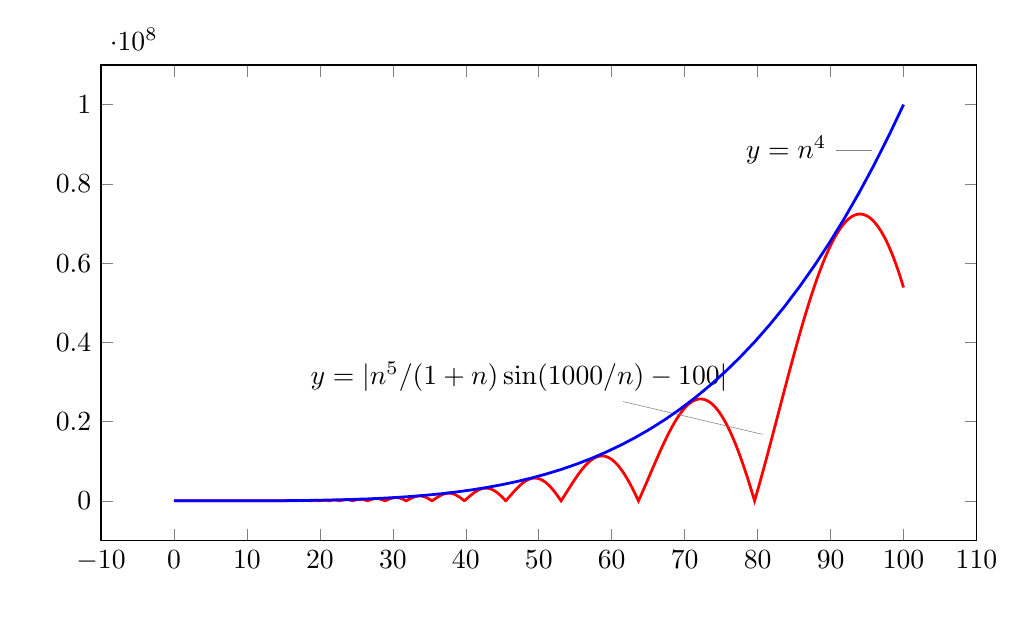
\begin{tikzpicture}[line width=1]
\begin{axis}[width=5in, height=3in,
             scatter/classes={a={mark=*,draw=black}},
             xlabel={\mbox{}},
             xlabel style={name=xlabel}, 
             ylabel={\mbox{}}, 
             legend style={
                at={(xlabel.south)},
                yshift=-1ex,
                anchor=north,
                legend cell align=left,
                },
        ]
]
\addplot[draw=red, line width=1] coordinates {(0.1001,100.0)
(0.2002,100.0)
(0.3003,100.0002)
(0.4004,99.9995)
(0.5005,100.0011)
(0.6006,100.0022)
(0.7007,99.9247)
(0.8008,100.1828)
(0.9009,100.2657)
(1.001,100.0133)
(1.1011,100.1992)
(1.2012,99.9749)
(1.3013,98.4725)
(1.4014,100.9381)
(1.5015,100.0538)
(1.6016,97.0887)
(1.7017,100.8896)
(1.8018,94.0809)
(1.9019,107.8044)
(2.002,99.8583)
(2.1021,112.8617)
(2.2022,83.9634)
(2.3023,85.839)
(2.4024,76.4811)
(2.5025,116.2298)
(2.6026,72.9149)
(2.7027,125.3258)
(2.8028,144.4373)
(2.9029,146.8884)
(3.003,100.5382)
(3.1031,31.9667)
(3.2032,173.8673)
(3.3033,17.1679)
(3.4034,203.329)
(3.5035,48.3478)
(3.6036,13.8306)
(3.7037,126.0836)
(3.8038,239.4049)
(3.9039,283.706)
(4.004,305.6579)
(4.1041,324.2276)
(4.2042,298.3106)
(4.3043,142.2508)
(4.4044,130.5626)
(4.5045,192.7602)
(4.6046,245.1909)
(4.7047,455.4141)
(4.8048,210.2191)
(4.9049,53.9576)
(5.005,598.2596)
(5.1051,407.1111)
(5.2052,383.3936)
(5.3053,103.3283)
(5.4054,149.718)
(5.5055,523.495)
(5.6056,425.5216)
(5.7057,657.1849)
(5.8058,403.4815)
(5.9059,431.2014)
(6.006,95.0801)
(6.1061,373.5935)
(6.2062,1107.0161)
(6.3063,1260.883)
(6.4064,1314.8029)
(6.5065,277.9063)
(6.6066,788.9728)
(6.7067,1847.7589)
(6.8068,1166.3514)
(6.9069,429.0041)
(7.007,2154.8827)
(7.1071,1284.444)
(7.2072,1077.1534)
(7.3073,2562.8448)
(7.4074,134.4053)
(7.5075,2563.0662)
(7.6076,1518.0771)
(7.7077,2613.5606)
(7.8078,2092.9521)
(7.9079,2370.9351)
(8.008,2693.6456)
(8.1081,2889.8701)
(8.2082,2484.5402)
(8.3083,3434.2696)
(8.4084,2050.9941)
(8.5085,4606.7571)
(8.6086,274.2684)
(8.7087,4994.0438)
(8.8088,2131.4163)
(8.9089,4355.5328)
(9.009,5226.074)
(9.1091,983.3496)
(9.2092,6256.1964)
(9.3093,3758.4852)
(9.4094,3728.1648)
(9.5095,7472.594)
(9.6096,3036.0765)
(9.7097,4985.0636)
(9.8098,8192.6014)
(9.9099,3134.1856)
(10.01,5484.942)
(10.1101,9595.8437)
(10.2102,5288.9201)
(10.3103,3902.7213)
(10.4104,10311.2312)
(10.5105,8594.8574)
(10.6106,128.9197)
(10.7107,9402.378)
(10.8108,12407.6204)
(10.9109,6832.4901)
(11.011,3727.6839)
(11.1111,12400.8448)
(11.2112,13579.235)
(11.3113,6340.1162)
(11.4114,5196.6271)
(11.5115,14462.3398)
(11.6116,16217.2099)
(11.7117,9331.249)
(11.8118,2794.3105)
(11.9119,14137.9183)
(12.012,19119.1102)
(12.1121,15229.9293)
(12.2122,4061.6674)
(12.3123,9571.866)
(12.4124,19842.8254)
(12.5125,22386.8464)
(12.6126,16011.7476)
(12.7127,3037.2035)
(12.8128,11730.4846)
(12.9129,22873.5879)
(13.013,26328.4345)
(13.1131,20743.8265)
(13.2132,7828.858)
(13.3133,8328.0032)
(13.4134,22652.4491)
(13.5135,30689.301)
(13.6136,29913.7809)
(13.7137,20391.4333)
(13.8138,4658.9945)
(13.9139,13068.6007)
(14.014,28089.1825)
(14.1141,36453.586)
(14.2142,35934.4824)
(14.3143,26508.1455)
(14.4144,10276.8264)
(14.5145,9099.917)
(14.6146,27291.2811)
(14.7147,40273.5492)
(14.8148,45180.8246)
(14.9149,40860.079)
(15.015,28042.3956)
(15.1151,9129.4627)
(15.2152,12329.9277)
(15.3153,32347.4708)
(15.4154,47240.5164)
(15.5155,54277.3593)
(15.6156,52117.749)
(15.7157,40990.3766)
(15.8158,22599.6637)
(15.9159,200.4889)
(16.016,23894.927)
(16.1161,44868.4877)
(16.2162,59949.4509)
(16.3163,66856.4708)
(16.4164,64492.4454)
(16.5165,53056.3329)
(16.6166,33972.1414)
(16.7167,9659.1518)
(16.8168,16813.9947)
(16.9169,42138.0052)
(17.017,63178.5121)
(17.1171,77347.3166)
(17.2172,82888.5133)
(17.3173,79052.7539)
(17.4174,66148.4122)
(17.5175,45473.3572)
(17.6176,19143.823)
(17.7177,10153.6622)
(17.8178,39455.7205)
(17.9179,65827.7256)
(18.018,86650.28)
(18.1181,99860.1303)
(18.2182,104125.9617)
(18.3183,98947.4895)
(18.4184,84674.4174)
(18.5185,62449.3939)
(18.6186,34085.4339)
(18.7187,1892.9828)
(18.8188,31525.3167)
(18.9189,63493.0585)
(19.019,91473.2682)
(19.1191,113259.9947)
(19.2192,127135.0898)
(19.3193,131980.8007)
(19.4194,127342.9442)
(19.5195,113443.5144)
(19.6196,91145.3152)
(19.7197,61874.3566)
(19.8198,27508.1748)
(19.9199,9760.1684)
(20.02,47571.8779)
(20.1201,83555.4885)
(20.2202,115473.3691)
(20.3203,141353.0837)
(20.4204,159596.6845)
(20.5205,169062.9212)
(20.6206,169119.3738)
(20.7207,159663.5061)
(20.8208,141113.4886)
(20.9209,114371.2546)
(21.021,80761.5679)
(21.1211,41951.8618)
(21.2212,141.7691)
(21.3213,43456.7616)
(21.4214,85888.8439)
(21.5215,125394.0689)
(21.6216,160083.385)
(21.7217,188305.7481)
(21.8218,208716.6351)
(21.9219,220329.7467)
(22.022,222550.6272)
(22.1221,215191.8374)
(22.2222,198470.156)
(22.3223,172987.0251)
(22.4224,139694.0704)
(22.5225,99846.0078)
(22.6226,54943.5889)
(22.7227,6669.4318)
(22.8228,43180.3465)
(22.9229,92765.844)
(23.023,140271.7408)
(23.1231,183971.8826)
(23.2232,222287.9668)
(23.3233,253840.587)
(23.4234,277491.2964)
(23.5235,292374.7655)
(23.6236,297920.5186)
(23.7237,293864.1258)
(23.8238,280248.0903)
(23.9239,257412.9898)
(24.024,225979.7059)
(24.1241,186823.8008)
(24.2242,141043.2658)
(24.3243,89920.988)
(24.4244,34883.3387)
(24.5245,22543.6903)
(24.6246,80779.4108)
(24.7247,138233.0958)
(24.8248,193347.1463)
(24.9249,244637.6684)
(25.025,290731.5119)
(25.1251,330398.9831)
(25.2252,362581.6136)
(25.3253,386414.54)
(25.4254,401243.2202)
(25.5255,406634.3742)
(25.6256,402381.1901)
(25.7257,388502.9758)
(25.8258,365239.5579)
(25.9259,333040.8387)
(26.026,292552.0031)
(26.1261,244594.9425)
(26.2262,190146.5057)
(26.3263,130314.2209)
(26.4264,66310.1468)
(26.5265,576.494)
(26.6266,69007.2594)
(26.7267,137622.4031)
(26.8268,205068.1918)
(26.9269,270023.1049)
(27.027,331222.4554)
(27.1271,387481.0298)
(27.2272,437713.4121)
(27.3273,480951.722)
(27.4274,516360.565)
(27.5275,543249.0585)
(27.6276,561079.8606)
(27.7277,569475.1872)
(27.8278,568219.8621)
(27.9279,557261.49)
(28.028,536707.8931)
(28.1281,506821.9862)
(28.2282,468014.3022)
(28.3283,420833.4028)
(28.4284,365954.4347)
(28.5285,304166.1019)
(28.6286,236356.3357)
(28.7287,163496.949)
(28.8288,86627.5576)
(28.9289,6839.0478)
(29.029,74743.1427)
(29.1291,156975.6732)
(29.2292,238713.6418)
(29.3293,318826.3981)
(29.4294,396212.6293)
(29.5295,469814.5428)
(29.6296,538630.9906)
(29.7297,601729.4082)
(29.8298,658256.4606)
(29.9299,707447.3145)
(30.03,748633.4799)
(30.1301,781249.1821)
(30.2302,804836.2539)
(30.3303,819047.5503)
(30.4304,823648.9121)
(30.5305,818519.7193)
(30.6306,803652.0908)
(30.7307,779148.8008)
(30.8308,745219.9936)
(30.9309,702178.7887)
(31.031,650435.8753)
(31.1311,590493.2034)
(31.2312,522936.8804)
(31.3313,448429.3877)
(31.4314,367701.2316)
(31.5315,281542.1433)
(31.6316,190791.9415)
(31.7317,96331.1678)
(31.8318,928.3975)
(31.9319,100053.2373)
(32.032,200097.5198)
(32.1321,300112.3503)
(32.2322,399154.7684)
(32.3323,496296.4133)
(32.4324,590631.7889)
(32.5325,681286.0651)
(32.6326,767422.3629)
(32.7327,848248.4765)
(32.8328,923022.9952)
(32.9329,991060.7928)
(33.033,1051737.8637)
(33.1331,1104495.489)
(33.2332,1148843.7235)
(33.3333,1184364.2024)
(33.4334,1210712.2714)
(33.5335,1227618.4494)
(33.6336,1234889.2402)
(33.7337,1232407.3119)
(33.8338,1220131.0688)
(33.9339,1198093.6443)
(34.034,1166401.3455)
(34.1341,1125231.5851)
(34.2342,1074830.3359)
(34.3343,1015509.1476)
(34.4344,947641.7672)
(34.5345,871660.4015)
(34.6346,788051.6665)
(34.7347,697352.2652)
(34.8348,600144.4351)
(34.9349,497051.2082)
(35.035,388731.5251)
(35.1351,275875.2418)
(35.2352,159198.0698)
(35.3353,39436.4856)
(35.4354,82657.3532)
(35.5355,206320.6522)
(35.6356,330784.9528)
(35.7357,455281.0023)
(35.8358,579043.4945)
(35.9359,701315.6549)
(36.036,821353.6471)
(36.1361,938430.7798)
(36.2362,1051841.4954)
(36.3363,1160905.1237)
(36.4364,1264969.3876)
(36.5365,1363413.6478)
(36.6366,1455651.8775)
(36.7367,1541135.3603)
(36.8368,1619355.1045)
(36.9369,1689843.9714)
(37.037,1752178.5162)
(37.1371,1805980.5411)
(37.2372,1850918.3627)
(37.3373,1886707.798)
(37.4374,1913112.8727)
(37.5375,1929946.2594)
(37.6376,1937069.4527)
(37.7377,1934392.6891)
(37.8378,1921874.6238)
(37.9379,1899521.7717)
(38.038,1867387.7274)
(38.1381,1825572.173)
(38.2382,1774219.6893)
(38.3383,1713518.3811)
(38.4384,1643698.3321)
(38.5385,1565029.9007)
(38.6386,1477821.8735)
(38.7387,1382419.4883)
(38.8388,1279202.3413)
(38.9389,1168582.1925)
(39.039,1051000.684)
(39.1391,926926.9828)
(39.2392,796855.3637)
(39.3393,661302.7441)
(39.4394,520806.1832)
(39.5395,375920.3597)
(39.6396,227215.0373)
(39.7397,75272.5315)
(39.8398,79314.8119)
(39.9399,235947.1174)
(40.04,394019.4477)
(40.1401,552924.2317)
(40.2402,712053.6422)
(40.3403,870801.9162)
(40.4404,1028567.6105)
(40.5405,1184755.7848)
(40.6406,1338780.1072)
(40.7407,1490064.875)
(40.8408,1638046.9477)
(40.9409,1782177.5856)
(41.041,1921924.1916)
(41.1411,2056771.9522)
(41.2412,2186225.3748)
(41.3413,2309809.7197)
(41.4414,2427072.3244)
(41.5415,2537583.8187)
(41.6416,2640939.2307)
(41.7417,2736758.983)
(41.8418,2824689.7785)
(41.9419,2904405.3773)
(42.042,2975607.2649)
(42.1421,3038025.2135)
(42.2422,3091417.7372)
(42.3423,3135572.4442)
(42.4424,3170306.2866)
(42.5425,3195465.7119)
(42.6426,3210926.7177)
(42.7427,3216594.8133)
(42.8428,3212404.8909)
(42.9429,3198321.0099)
(43.043,3174336.0975)
(43.1431,3140471.5704)
(43.2432,3096776.879)
(43.3433,3043328.9808)
(43.4434,2980231.7445)
(43.5435,2907615.2901)
(43.6436,2825635.2691)
(43.7437,2734472.088)
(43.8438,2634330.0796)
(43.9439,2525436.6271)
(44.044,2408041.243)
(44.1441,2282414.6093)
(44.2442,2148847.5809)
(44.3443,2007650.1572)
(44.4444,1859150.4264)
(44.5445,1703693.4843)
(44.6446,1541640.3338)
(44.7447,1373366.7666)
(44.8448,1199262.2325)
(44.9449,1019728.6981)
(45.045,835179.4996)
(45.1451,646038.1924)
(45.2452,452737.4003)
(45.3453,255717.6676)
(45.4454,55426.3176)
(45.5455,147683.6808)
(45.6456,353154.8356)
(45.7457,560526.2397)
(45.8458,769334.6635)
(45.9459,979115.6291)
(46.046,1189404.464)
(46.1461,1399737.3324)
(46.2462,1609652.243)
(46.3463,1818690.0298)
(46.4464,2026395.3067)
(46.5465,2232317.3927)
(46.6466,2436011.2064)
(46.7467,2637038.1306)
(46.8468,2834966.8429)
(46.9469,3029374.1142)
(47.047,3219845.5723)
(47.1471,3405976.4309)
(47.2472,3587372.1833)
(47.3473,3763649.2597)
(47.4474,3934435.6485)
(47.5475,4099371.481)
(47.6476,4258109.5786)
(47.7477,4410315.9642)
(47.8478,4555670.3354)
(47.9479,4693866.5018)
(48.048,4824612.7851)
(48.1481,4947632.3825)
(48.2482,5062663.6946)
(48.3483,5169460.6167)
(48.4484,5267792.7952)
(48.5485,5357445.8488)
(48.6486,5438221.5556)
(48.7487,5509938.0063)
(48.8488,5572429.7244)
(48.9489,5625547.7539)
(49.049,5669159.7157)
(49.1491,5703149.8324)
(49.2492,5727418.9243)
(49.3493,5741884.375)
(49.4494,5746480.0692)
(49.5495,5741156.3035)
(49.6496,5725879.6702)
(49.7497,5700632.9156)
(49.8498,5665414.7744)
(49.9499,5620239.7795)
(50.0501,5565138.0503)
(50.1502,5500155.0589)
(50.2503,5425351.3754)
(50.3504,5340802.3947)
(50.4505,5246598.0435)
(50.5506,5142842.4708)
(50.6507,5029653.7214)
(50.7508,4907163.3937)
(50.8509,4775516.2837)
(50.951,4634870.0146)
(51.0511,4485394.6548)
(51.1512,4327272.3232)
(51.2513,4160696.7849)
(51.3514,3985873.0369)
(51.4515,3803016.8847)
(51.5516,3612354.5114)
(51.6517,3414122.0401)
(51.7518,3208565.0893)
(51.8519,2995938.3245)
(51.952,2776505.0041)
(52.0521,2550536.5223)
(52.1522,2318311.9495)
(52.2523,2080117.5701)
(52.3524,1836246.4195)
(52.4525,1586997.8204)
(52.5526,1332676.9192)
(52.6527,1073594.2234)
(52.7528,810065.1406)
(52.8529,542409.5193)
(52.953,270951.1924)
(53.0531,3982.4751)
(53.1532,282061.0358)
(53.2533,562951.4043)
(53.3534,846318.2971)
(53.4535,1131824.6667)
(53.5536,1419132.1302)
(53.6537,1707901.3919)
(53.7538,1997792.6579)
(53.8539,2288466.0455)
(53.954,2579581.9834)
(54.0541,2870801.6052)
(54.1542,3161787.1343)
(54.2543,3452202.2602)
(54.3544,3741712.5071)
(54.4545,4029985.592)
(54.5546,4316691.7751)
(54.6547,4601504.1997)
(54.7548,4884099.2232)
(54.8549,5164156.7381)
(54.955,5441360.4828)
(55.0551,5715398.3429)
(55.1552,5985962.6419)
(55.2553,6252750.4217)
(55.3554,6515463.7129)
(55.4555,6773809.7944)
(55.5556,7027501.443)
(55.6557,7276257.1718)
(55.7558,7519801.4585)
(55.8559,7757864.9633)
(55.956,7990184.7359)
(56.0561,8216504.4123)
(56.1562,8436574.4004)
(56.2563,8650152.0566)
(56.3564,8857001.8503)
(56.4565,9056895.5196)
(56.5566,9249612.2156)
(56.6567,9434938.6372)
(56.7568,9612669.1561)
(56.8569,9782605.9309)
(56.957,9944559.0121)
(57.0571,10098346.4377)
(57.1572,10243794.3184)
(57.2573,10380736.9137)
(57.3574,10509016.6993)
(57.4575,10628484.4245)
(57.5576,10738999.1611)
(57.6577,10840428.3436)
(57.7578,10932647.8005)
(57.8579,11015541.7775)
(57.958,11089002.9518)
(58.0581,11152932.4389)
(58.1582,11207239.7917)
(58.2583,11251842.9908)
(58.3584,11286668.4285)
(58.4585,11311650.8849)
(58.5586,11326733.4968)
(58.6587,11331867.7198)
(58.7588,11327013.2838)
(58.8589,11312138.1419)
(58.959,11287218.4127)
(59.0591,11252238.3169)
(59.1592,11207190.1079)
(59.2593,11152073.9963)
(59.3594,11086898.0694)
(59.4595,11011678.2052)
(59.5596,10926437.9813)
(59.6597,10831208.5784)
(59.7598,10726028.6806)
(59.8599,10610944.3692)
(59.96,10486009.0136)
(60.0601,10351283.1581)
(60.1602,10206834.4035)
(60.2603,10052737.2867)
(60.3604,9889073.1557)
(60.4605,9715930.0414)
(60.5606,9533402.5265)
(60.6607,9341591.6117)
(60.7608,9140604.578)
(60.8609,8930554.848)
(60.961,8711561.8436)
(61.0611,8483750.8415)
(61.1612,8247252.8278)
(61.2613,8002204.3491)
(61.3614,7748747.363)
(61.4615,7487029.0866)
(61.5616,7217201.8433)
(61.6617,6939422.9095)
(61.7618,6653854.3585)
(61.8619,6360662.9047)
(61.962,6060019.7467)
(62.0621,5752100.4094)
(62.1622,5437084.5862)
(62.2623,5115155.98)
(62.3624,4786502.1444)
(62.4625,4451314.325)
(62.5626,4109787.3004)
(62.6627,3762119.223)
(62.7628,3408511.4607)
(62.8629,3049168.4383)
(62.963,2684297.4801)
(63.0631,2314108.6523)
(63.1632,1938814.6064)
(63.2633,1558630.4237)
(63.3634,1173773.4598)
(63.4635,784463.1914)
(63.5636,390921.0623)
(63.6637,6629.6672)
(63.7638,407964.072)
(63.8639,812855.7107)
(63.964,1221076.7738)
(64.0641,1632398.2301)
(64.1642,2046589.9716)
(64.2643,2463420.9569)
(64.3644,2882659.3527)
(64.4645,3304072.6739)
(64.5646,3727427.9217)
(64.6647,4152491.7199)
(64.7648,4579030.4493)
(64.8649,5006810.3803)
(64.965,5435597.8034)
(65.0651,5865159.1577)
(65.1652,6295261.1573)
(65.2653,6725670.9156)
(65.3654,7156156.0675)
(65.4655,7586484.8893)
(65.5656,8016426.4167)
(65.6657,8445750.56)
(65.7658,8874228.2178)
(65.8659,9301631.3876)
(65.966,9727733.2747)
(66.0661,10152308.3984)
(66.1662,10575132.6964)
(66.2663,10995983.6257)
(66.3664,11414640.2625)
(66.4665,11830883.3989)
(66.5666,12244495.6371)
(66.6667,12655261.4821)
(66.7668,13062967.4306)
(66.8669,13467402.0587)
(66.967,13868356.1067)
(67.0671,14265622.5615)
(67.1672,14658996.7364)
(67.2673,15048276.3492)
(67.3674,15433261.5966)
(67.4675,15813755.2277)
(67.5676,16189562.6141)
(67.6677,16560491.818)
(67.7678,16926353.6576)
(67.8679,17286961.7707)
(67.968,17642132.6753)
(68.0681,17991685.8284)
(68.1682,18335443.6823)
(68.2683,18673231.7384)
(68.3684,19004878.5988)
(68.4685,19330216.0161)
(68.5686,19649078.94)
(68.6687,19961305.5627)
(68.7688,20266737.3612)
(68.8689,20565219.1381)
(68.969,20856599.0599)
(69.0691,21140728.6931)
(69.1692,21417463.0382)
(69.2693,21686660.5622)
(69.3694,21948183.2278)
(69.4695,22201896.5219)
(69.5696,22447669.4809)
(69.6697,22685374.7151)
(69.7698,22914888.4303)
(69.8699,23136090.4478)
(69.97,23348864.2227)
(70.0701,23553096.8596)
(70.1702,23748679.1275)
(70.2703,23935505.4719)
(70.3704,24113474.0257)
(70.4705,24282486.6182)
(70.5706,24442448.7824)
(70.6707,24593269.7603)
(70.7708,24734862.5069)
(70.8709,24867143.6925)
(70.971,24990033.7034)
(71.0711,25103456.6408)
(71.1712,25207340.3181)
(71.2713,25301616.2575)
(71.3714,25386219.684)
(71.4715,25461089.5187)
(71.5716,25526168.3704)
(71.6717,25581402.5258)
(71.7718,25626741.9385)
(71.8719,25662140.2167)
(71.972,25687554.6091)
(72.0721,25702945.9903)
(72.1722,25708278.8446)
(72.2723,25703521.2482)
(72.3724,25688644.8513)
(72.4725,25663624.8576)
(72.5726,25628440.0041)
(72.6727,25583072.5391)
(72.7728,25527508.199)
(72.8729,25461736.1846)
(72.973,25385749.1361)
(73.0731,25299543.1071)
(73.1732,25203117.538)
(73.2733,25096475.2279)
(73.3734,24979622.3065)
(73.4735,24852568.2043)
(73.5736,24715325.6224)
(73.6737,24567910.5016)
(73.7738,24410341.9907)
(73.8739,24242642.4135)
(73.974,24064837.2362)
(74.0741,23876955.033)
(74.1742,23679027.4519)
(74.2743,23471089.1794)
(74.3744,23253177.9047)
(74.4745,23025334.2834)
(74.5746,22787601.9006)
(74.6747,22540027.2337)
(74.7748,22282659.6141)
(74.8749,22015551.1893)
(74.975,21738756.8835)
(75.0751,21452334.3592)
(75.1752,21156343.9765)
(75.2753,20850848.7542)
(75.3754,20535914.3285)
(75.4755,20211608.9128)
(75.5756,19878003.2565)
(75.6757,19535170.6038)
(75.7758,19183186.652)
(75.8759,18822129.5096)
(75.976,18452079.6547)
(76.0761,18073119.892)
(76.1762,17685335.3109)
(76.2763,17288813.2429)
(76.3764,16883643.2182)
(76.4765,16469916.9237)
(76.5766,16047728.1591)
(76.6767,15617172.7943)
(76.7768,15178348.7263)
(76.8769,14731355.8355)
(76.977,14276295.9424)
(77.0771,13813272.7649)
(77.1772,13342391.8742)
(77.2773,12863760.6519)
(77.3774,12377488.2465)
(77.4775,11883685.53)
(77.5776,11382465.0549)
(77.6777,10873941.0109)
(77.7778,10358229.1817)
(77.8779,9835446.902)
(77.978,9305713.0147)
(78.0781,8769147.8278)
(78.1782,8225873.0722)
(78.2783,7676011.8586)
(78.3784,7119688.6353)
(78.4785,6557029.1463)
(78.5786,5988160.3887)
(78.6787,5413210.5711)
(78.7788,4832309.0719)
(78.8789,4245586.398)
(78.979,3653174.1431)
(79.0791,3055204.9469)
(79.1792,2451812.4545)
(79.2793,1843131.2754)
(79.3794,1229296.9437)
(79.4795,610445.8774)
(79.5796,13284.6606)
(79.6797,641756.6028)
(79.7798,1274831.1156)
(79.8799,1912368.6387)
(79.98,2554228.9236)
(80.0801,3200271.072)
(80.1802,3850353.5736)
(80.2803,4504334.344)
(80.3804,5162070.762)
(80.4805,5823419.7066)
(80.5806,6488237.5938)
(80.6807,7156380.4129)
(80.7808,7827703.7625)
(80.8809,8502062.8863)
(80.981,9179312.7082)
(81.0811,9859307.8673)
(81.1812,10541902.7529)
(81.2813,11226951.538)
(81.3814,11914308.2137)
(81.4815,12603826.6224)
(81.5816,13295360.4911)
(81.6817,13988763.4639)
(81.7818,14683889.1345)
(81.8819,15380591.0782)
(81.982,16078722.8829)
(82.0821,16778138.1812)
(82.1822,17478690.6802)
(82.2823,18180234.1926)
(82.3824,18882622.6663)
(82.4825,19585710.2138)
(82.5826,20289351.1421)
(82.6827,20993399.9804)
(82.7828,21697711.5095)
(82.8829,22402140.7891)
(82.983,23106543.1854)
(83.0831,23810774.3985)
(83.1832,24514690.4891)
(83.2833,25218147.9046)
(83.3834,25921003.5051)
(83.4835,26623114.5891)
(83.5836,27324338.9184)
(83.6837,28024534.7427)
(83.7838,28723560.8243)
(83.8839,29421276.4616)
(83.984,30117541.5126)
(84.0841,30812216.4181)
(84.1842,31505162.2245)
(84.2843,32196240.6056)
(84.3844,32885313.8849)
(84.4845,33572245.0567)
(84.5846,34256897.8075)
(84.6847,34939136.5362)
(84.7848,35618826.375)
(84.8849,36295833.2086)
(84.985,36970023.6938)
(85.0851,37641265.2789)
(85.1852,38309426.222)
(85.2853,38974375.6095)
(85.3854,39635983.3738)
(85.4855,40294120.311)
(85.5856,40948658.0978)
(85.6857,41599469.3084)
(85.7858,42246427.4308)
(85.8859,42889406.8828)
(85.986,43528283.0273)
(86.0861,44162932.1881)
(86.1862,44793231.6643)
(86.2863,45419059.7448)
(86.3864,46040295.7226)
(86.4865,46656819.9084)
(86.5866,47268513.6443)
(86.6867,47875259.3161)
(86.7868,48476940.3669)
(86.8869,49073441.3088)
(86.987,49664647.7348)
(87.0871,50250446.3311)
(87.1872,50830724.8874)
(87.2873,51405372.3089)
(87.3874,51974278.6259)
(87.4875,52537335.0048)
(87.5876,53094433.7575)
(87.6877,53645468.3515)
(87.7878,54190333.4185)
(87.8879,54728924.7642)
(87.988,55261139.3761)
(88.0881,55786875.4324)
(88.1882,56306032.3095)
(88.2883,56818510.5902)
(88.3884,57324212.0707)
(88.4885,57823039.7678)
(88.5886,58314897.9256)
(88.6887,58799692.0219)
(88.7888,59277328.7749)
(88.8889,59747716.1482)
(88.989,60210763.3571)
(89.0891,60666380.8737)
(89.1892,61114480.4317)
(89.2893,61554975.0317)
(89.3894,61987778.9449)
(89.4895,62412807.718)
(89.5896,62829978.1769)
(89.6897,63239208.4301)
(89.7898,63640417.8726)
(89.8899,64033527.1885)
(89.99,64418458.3545)
(90.0901,64795134.6421)
(90.1902,65163480.62)
(90.2903,65523422.1565)
(90.3904,65874886.4214)
(90.4905,66217801.8872)
(90.5906,66552098.3314)
(90.6907,66877706.8368)
(90.7908,67194559.793)
(90.8909,67502590.897)
(90.991,67801735.1539)
(91.0911,68091928.877)
(91.1912,68373109.6878)
(91.2913,68645216.5164)
(91.3914,68908189.6005)
(91.4915,69161970.4853)
(91.5916,69406502.023)
(91.6917,69641728.371)
(91.7918,69867594.9917)
(91.8919,70084048.6508)
(91.992,70291037.4156)
(92.0921,70488510.6536)
(92.1922,70676419.0307)
(92.2923,70854714.5088)
(92.3924,71023350.3438)
(92.4925,71182281.0831)
(92.5926,71331462.5632)
(92.6927,71470851.9066)
(92.7928,71600407.5194)
(92.8929,71720089.0877)
(92.993,71829857.5748)
(93.0931,71929675.2176)
(93.1932,72019505.523)
(93.2933,72099313.2644)
(93.3934,72169064.4777)
(93.4935,72228726.4577)
(93.5936,72278267.7533)
(93.6937,72317658.1638)
(93.7938,72346868.7344)
(93.8939,72365871.7515)
(93.994,72374640.7384)
(94.0941,72373150.4499)
(94.1942,72361376.8682)
(94.2943,72339297.1971)
(94.3944,72306889.8574)
(94.4945,72264134.4814)
(94.5946,72211011.9075)
(94.6947,72147504.175)
(94.7948,72073594.5181)
(94.8949,71989267.3603)
(94.995,71894508.3088)
(95.0951,71789304.1486)
(95.1952,71673642.8362)
(95.2953,71547513.4936)
(95.3954,71410906.4023)
(95.4955,71263812.9968)
(95.5956,71106225.8585)
(95.6957,70938138.7088)
(95.7958,70759546.403)
(95.8959,70570444.9232)
(95.996,70370831.3723)
(96.0961,70160703.9664)
(96.1962,69940062.0285)
(96.2963,69708905.9813)
(96.3964,69467237.3405)
(96.4965,69215058.7072)
(96.5966,68952373.7614)
(96.6967,68679187.2542)
(96.7968,68395505.0011)
(96.8969,68101333.874)
(96.997,67796681.7947)
(97.0971,67481557.7265)
(97.1972,67155971.6675)
(97.2973,66819934.6426)
(97.3974,66473458.6961)
(97.4975,66116556.8838)
(97.5976,65749243.2657)
(97.6977,65371532.8979)
(97.7978,64983441.8252)
(97.8979,64584987.073)
(97.998,64176186.6392)
(98.0981,63757059.4871)
(98.1982,63327625.5366)
(98.2983,62887905.6567)
(98.3984,62437921.6576)
(98.4985,61977696.2822)
(98.5986,61507253.1986)
(98.6987,61026616.9914)
(98.7988,60535813.1543)
(98.8989,60034868.0814)
(98.999,59523809.0592)
(99.0991,59002664.2584)
(99.1992,58471462.7261)
(99.2993,57930234.3768)
(99.3994,57379009.9849)
(99.4995,56817821.1759)
(99.5996,56246700.4187)
(99.6997,55665681.0167)
(99.7998,55074797.1001)
(99.8999,54474083.617)
(100.0,53863576.3257)};\node[pin=above left:{$y=|n^5/(1+n) \sin(1000/n) - 100|$}] at (axis cs:82,16204527.16254407) {};\addplot[draw=blue, line width=1] coordinates {(0.0,0.0)
(2.0408,17.3467)
(4.0816,277.5464)
(6.1224,1405.0789)
(8.1633,4440.7431)
(10.2041,10841.6578)
(12.2449,22481.2617)
(14.2857,41649.3128)
(16.3265,71051.8889)
(18.3673,113811.3874)
(20.4082,173466.5256)
(22.449,253972.3401)
(24.4898,359700.1874)
(26.5306,495437.7436)
(28.5714,666389.0046)
(30.6122,878174.2856)
(32.6531,1136830.2219)
(34.6939,1448809.7681)
(36.7347,1820982.1987)
(38.7755,2260633.1077)
(40.8163,2775464.4089)
(42.8571,3373594.3357)
(44.898,4063557.4411)
(46.9388,4854304.5979)
(48.9796,5755202.9983)
(51.0204,6776036.1546)
(53.0612,7927003.8983)
(55.102,9218722.3809)
(57.1429,10662224.0733)
(59.1837,12268957.7663)
(61.2245,14050788.5702)
(63.2653,16019997.9149)
(65.3061,18189283.5503)
(67.3469,20571759.5456)
(69.3878,23180956.2897)
(71.4286,26030820.4915)
(73.4694,29135715.1791)
(75.5102,32510419.7005)
(77.551,36170129.7235)
(79.5918,40130457.2352)
(81.6327,44407430.5427)
(83.6735,49017494.2726)
(85.7143,53977509.3711)
(87.7551,59304753.1042)
(89.7959,65016919.0576)
(91.8367,71132117.1364)
(93.8776,77668873.5656)
(95.9184,84646130.8899)
(97.9592,92083247.9733)
(100.0,100000000.0)};\node[pin=left:{$y=n^4$}] at (axis cs:97,88529281) {};
\end{axis}\end{tikzpicture}\end{center}

%-*-latex-*-

\begin{center}
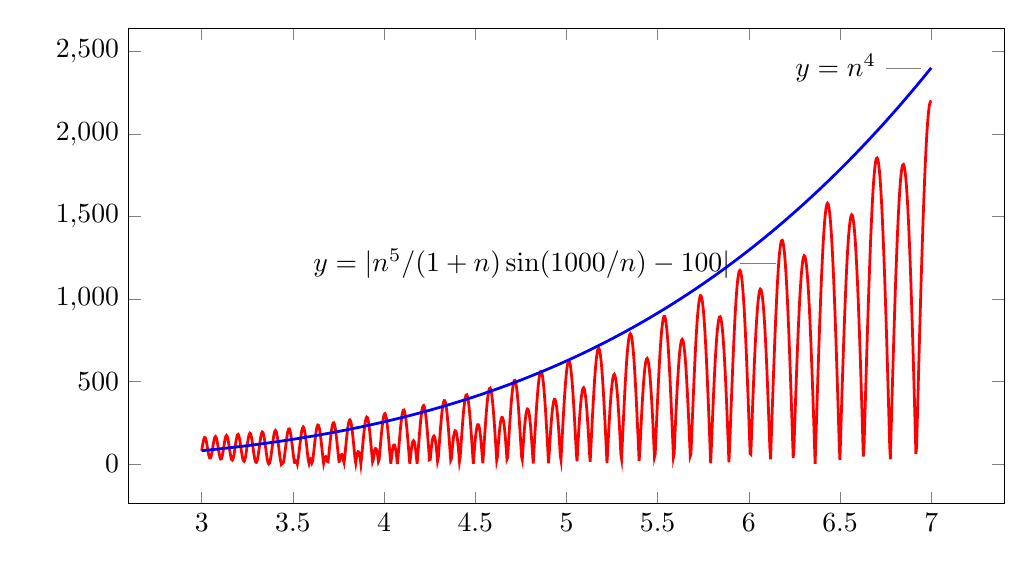
\begin{tikzpicture}[line width=1]
\begin{axis}[width=5in, height=3in,
             scatter/classes={a={mark=*,draw=black}},
             xlabel={\mbox{}},
             xlabel style={name=xlabel}, 
             ylabel={\mbox{}}, 
             legend style={
                at={(xlabel.south)},
                yshift=-1ex,
                anchor=north,
                legend cell align=left,
                },
        ]
]
\addplot[draw=red, line width=1] coordinates {(3.0,80.6301)
(3.004,107.3008)
(3.008,132.7879)
(3.012,152.1556)
(3.016,161.6538)
(3.02,159.4284)
(3.024,145.8614)
(3.028,123.483)
(3.032,96.4803)
(3.036,69.9005)
(3.04,48.7036)
(3.044,36.8426)
(3.048,36.5403)
(3.0521,47.8931)
(3.0561,68.8678)
(3.0601,95.6852)
(3.0641,123.5163)
(3.0681,147.3573)
(3.0721,162.9271)
(3.0761,167.4241)
(3.0801,160.0131)
(3.0841,141.9589)
(3.0881,116.3902)
(3.0921,87.7417)
(3.0961,60.975)
(3.1001,40.7188)
(3.1041,30.4755)
(3.1081,32.0305)
(3.1121,45.16)
(3.1161,67.6821)
(3.1201,95.8374)
(3.1241,124.9296)
(3.1281,150.1137)
(3.1321,167.2007)
(3.1361,173.3442)
(3.1401,167.4988)
(3.1441,150.5785)
(3.1481,125.2953)
(3.1522,95.7087)
(3.1562,66.5638)
(3.1602,42.5272)
(3.1642,27.4442)
(3.1682,23.7351)
(3.1722,32.0227)
(3.1762,51.0469)
(3.1802,77.8734)
(3.1842,108.361)
(3.1882,137.8095)
(3.1922,161.686)
(3.1962,176.3181)
(3.2002,179.4469)
(3.2042,170.5604)
(3.2082,150.9589)
(3.2122,123.5483)
(3.2162,92.3955)
(3.2202,62.1167)
(3.2242,37.1912)
(3.2282,21.3035)
(3.2322,16.809)
(3.2362,24.3995)
(3.2402,43.0139)
(3.2442,70.0026)
(3.2482,101.5182)
(3.2523,133.0731)
(3.2563,160.1813)
(3.2603,178.9934)
(3.2643,186.8342)
(3.2683,182.5699)
(3.2723,166.7562)
(3.2763,141.5504)
(3.2803,110.4031)
(3.2843,77.5755)
(3.2883,47.5516)
(3.2923,24.4266)
(3.2963,11.3545)
(3.3003,10.1293)
(3.3043,20.9528)
(3.3083,42.4179)
(3.3123,71.7064)
(3.3163,104.9699)
(3.3203,137.8434)
(3.3243,166.0202)
(3.3283,185.8126)
(3.3323,194.6268)
(3.3363,191.2905)
(3.3403,176.1945)
(3.3443,151.2328)
(3.3483,119.5522)
(3.3524,85.145)
(3.3564,52.3413)
(3.3604,25.2625)
(3.3644,7.3084)
(3.3684,0.739)
(3.3724,6.4023)
(3.3764,23.6384)
(3.3804,50.3701)
(3.3844,83.3656)
(3.3884,118.6375)
(3.3924,151.9301)
(3.3964,179.2324)
(3.4004,197.2574)
(3.4044,203.8288)
(3.4084,198.1324)
(3.4124,180.8035)
(3.4164,153.8434)
(3.4204,120.3766)
(3.4244,84.28)
(3.4284,49.7289)
(3.4324,20.7136)
(3.4364,0.5824)
(3.4404,8.3373)
(3.4444,4.9971)
(3.4484,10.2613)
(3.4525,35.7536)
(3.4565,68.6498)
(3.4605,105.2979)
(3.4645,141.6345)
(3.4685,173.6374)
(3.4725,197.7682)
(3.4765,211.3574)
(3.4805,212.8906)
(3.4845,202.1656)
(3.4885,180.3064)
(3.4925,149.634)
(3.4965,113.4102)
(3.5005,75.4839)
(3.5045,39.8785)
(3.5085,10.3655)
(3.5125,9.9307)
(3.5165,18.8568)
(3.5205,15.4484)
(3.5245,0.0237)
(3.5285,25.8576)
(3.5325,59.5624)
(3.5365,97.6605)
(3.5405,136.2791)
(3.5445,171.4987)
(3.5485,199.7499)
(3.5526,218.1699)
(3.5566,224.8853)
(3.5606,219.1929)
(3.5646,201.6223)
(3.5686,173.8762)
(3.5726,138.6559)
(3.5766,99.3902)
(3.5806,59.8971)
(3.5846,24.0105)
(3.5886,4.7904)
(3.5926,23.7139)
(3.5966,30.9188)
(3.6006,25.6848)
(3.6046,8.4739)
(3.6086,19.1203)
(3.6126,54.5295)
(3.6166,94.4571)
(3.6206,135.1902)
(3.6246,172.9471)
(3.6286,204.2271)
(3.6326,226.1318)
(3.6366,236.6266)
(3.6406,234.7218)
(3.6446,220.556)
(3.6486,195.377)
(3.6527,161.4229)
(3.6567,121.715)
(3.6607,79.7841)
(3.6647,39.3526)
(3.6687,4.0047)
(3.6727,23.1296)
(3.6767,39.6459)
(3.6807,44.0716)
(3.6847,35.9883)
(3.6887,16.0623)
(3.6927,14.0198)
(3.6967,51.7017)
(3.7007,93.7812)
(3.7047,136.6867)
(3.7087,176.782)
(3.7127,210.6742)
(3.7167,235.497)
(3.7207,249.1478)
(3.7247,250.4585)
(3.7287,239.2871)
(3.7327,216.523)
(3.7367,184.0086)
(3.7407,144.3819)
(3.7447,100.8571)
(3.7487,56.9603)
(3.7528,16.2418)
(3.7568,18.0094)
(3.7608,43.0283)
(3.7648,56.7919)
(3.7688,58.1751)
(3.7728,47.0357)
(3.7768,24.2188)
(3.7808,8.5143)
(3.7848,48.6298)
(3.7888,93.0229)
(3.7928,138.2618)
(3.7968,180.8549)
(3.8008,217.5193)
(3.8048,245.4316)
(3.8088,262.4398)
(3.8128,267.2237)
(3.8168,259.3893)
(3.8208,239.4936)
(3.8248,208.9974)
(3.8288,170.1507)
(3.8328,125.8212)
(3.8368,79.2783)
(3.8408,33.9493)
(3.8448,6.8327)
(3.8488,40.0725)
(3.8529,63.3289)
(3.8569,74.8889)
(3.8609,73.8868)
(3.8649,60.3624)
(3.8689,35.2526)
(3.8729,0.3194)
(3.8769,41.9796)
(3.8809,88.6695)
(3.8849,136.4703)
(3.8889,182.0294)
(3.8929,222.1557)
(3.8969,254.0415)
(3.9009,275.4548)
(3.9049,284.8899)
(3.9089,281.6676)
(3.9129,265.9763)
(3.9169,238.8548)
(3.9209,202.117)
(3.9249,158.2243)
(3.9289,110.1168)
(3.9329,61.0127)
(3.9369,14.1921)
(3.9409,27.222)
(3.9449,60.47)
(3.9489,83.3356)
(3.953,94.2887)
(3.957,92.582)
(3.961,78.295)
(3.965,52.3248)
(3.969,16.3231)
(3.973,27.4144)
(3.977,76.0987)
(3.981,126.6288)
(3.985,175.7909)
(3.989,220.4628)
(3.993,257.8109)
(3.997,285.4666)
(4.001,301.6723)
(4.005,305.388)
(4.009,296.3518)
(4.013,275.0921)
(4.017,242.8903)
(4.021,201.6982)
(4.025,154.0149)
(4.029,102.7313)
(4.033,50.9527)
(4.037,1.8094)
(4.041,41.7316)
(4.045,77.044)
(4.049,101.9971)
(4.0531,115.0802)
(4.0571,115.4885)
(4.0611,103.1673)
(4.0651,78.8105)
(4.0691,43.8164)
(4.0731,0.2022)
(4.0771,49.5171)
(4.0811,102.4763)
(4.0851,155.6278)
(4.0891,205.9177)
(4.0931,250.46)
(4.0971,286.7012)
(4.1011,312.5629)
(4.1051,326.5568)
(4.1091,327.8659)
(4.1131,316.3864)
(4.1171,292.7298)
(4.1211,258.1848)
(4.1251,214.6425)
(4.1291,164.4885)
(4.1331,110.4688)
(4.1371,55.5373)
(4.1411,2.6934)
(4.1451,45.1816)
(4.1491,85.4802)
(4.1532,116.0076)
(4.1572,135.0984)
(4.1612,141.7023)
(4.1652,135.4373)
(4.1692,116.6064)
(4.1732,86.1779)
(4.1772,45.7307)
(4.1812,2.6317)
(4.1852,56.3946)
(4.1892,112.765)
(4.1932,168.8185)
(4.1972,221.6516)
(4.2012,268.5311)
(4.2052,307.0337)
(4.2092,335.1686)
(4.2132,351.4767)
(4.2172,355.102)
(4.2212,345.8315)
(4.2252,324.1029)
(4.2292,290.979)
(4.2332,248.0916)
(4.2372,197.5565)
(4.2412,141.8663)
(4.2452,83.7654)
(4.2492,26.1125)
(4.2533,28.2595)
(4.2573,76.6825)
(4.2613,116.7823)
(4.2653,146.5924)
(4.2693,164.6468)
(4.2733,170.0483)
(4.2773,162.5089)
(4.2813,142.3597)
(4.2853,110.5325)
(4.2893,68.5123)
(4.2933,18.2642)
(4.2973,37.8619)
(4.3013,97.2434)
(4.3053,157.1092)
(4.3093,214.6698)
(4.3133,267.2465)
(4.3173,312.3953)
(4.3213,348.0182)
(4.3253,372.4574)
(4.3293,384.5695)
(4.3333,383.7746)
(4.3373,370.0799)
(4.3413,344.0763)
(4.3453,306.9088)
(4.3493,260.2224)
(4.3534,206.0855)
(4.3574,146.896)
(4.3614,85.2727)
(4.3654,23.9383)
(4.3694,34.4011)
(4.3734,87.1747)
(4.3774,132.0594)
(4.3814,167.0793)
(4.3854,190.6904)
(4.3894,201.8448)
(4.3934,200.0335)
(4.3974,185.306)
(4.4014,158.2648)
(4.4054,120.037)
(4.4094,72.224)
(4.4134,16.8312)
(4.4174,43.8192)
(4.4214,107.1869)
(4.4254,170.6214)
(4.4294,231.473)
(4.4334,287.2037)
(4.4374,335.4909)
(4.4414,374.3232)
(4.4454,402.0813)
(4.4494,417.6022)
(4.4535,420.225)
(4.4575,409.8148)
(4.4615,386.7659)
(4.4655,351.9832)
(4.4695,306.8427)
(4.4735,253.1347)
(4.4775,192.9894)
(4.4815,128.7909)
(4.4855,63.0805)
(4.4895,1.5438)
(4.4935,62.5309)
(4.4975,117.476)
(4.5015,164.2142)
(4.5055,200.9042)
(4.5095,226.0977)
(4.5135,238.7939)
(4.5175,238.4759)
(4.5215,225.1283)
(4.5255,199.2349)
(4.5295,161.7584)
(4.5335,114.1009)
(4.5375,58.0486)
(4.5415,4.2974)
(4.5455,70.6018)
(4.5495,138.3842)
(4.5536,205.1122)
(4.5576,268.2964)
(4.5616,325.5824)
(4.5656,374.8375)
(4.5696,414.2278)
(4.5736,442.285)
(4.5776,457.9574)
(4.5816,460.6472)
(4.5856,450.2291)
(4.5896,427.0534)
(4.5936,391.9305)
(4.5976,346.0997)
(4.6016,291.1825)
(4.6056,229.1229)
(4.6096,162.1169)
(4.6136,92.5325)
(4.6176,22.8261)
(4.6216,44.5454)
(4.6256,107.2101)
(4.6296,162.9645)
(4.6336,209.8491)
(4.6376,246.2153)
(4.6416,270.7814)
(4.6456,282.6747)
(4.6496,281.4598)
(4.6537,267.1514)
(4.6577,240.2115)
(4.6617,201.5317)
(4.6657,152.4008)
(4.6697,94.4591)
(4.6737,29.642)
(4.6777,39.8873)
(4.6817,111.8104)
(4.6857,183.7325)
(4.6897,253.2619)
(4.6937,318.0896)
(4.6977,376.0649)
(4.7017,425.2658)
(4.7057,464.0603)
(4.7097,491.1593)
(4.7137,505.6559)
(4.7177,507.054)
(4.7217,495.2818)
(4.7257,470.6922)
(4.7297,434.0498)
(4.7337,386.504)
(4.7377,329.5507)
(4.7417,264.9831)
(4.7457,194.8333)
(4.7497,121.3072)
(4.7538,46.7139)
(4.7578,26.6072)
(4.7618,96.3595)
(4.7658,160.3609)
(4.7698,216.6108)
(4.7738,263.3515)
(4.7778,299.1212)
(4.7818,322.7975)
(4.7858,333.6301)
(4.7898,331.2626)
(4.7938,315.7407)
(4.7978,287.5096)
(4.8018,247.3981)
(4.8058,196.5923)
(4.8098,136.5981)
(4.8138,69.1945)
(4.8178,3.6207)
(4.8218,79.6913)
(4.8258,156.7676)
(4.8298,232.573)
(4.8338,304.8715)
(4.8378,371.5331)
(4.8418,430.5955)
(4.8458,480.3208)
(4.8498,519.2448)
(4.8539,546.2183)
(4.8579,560.4387)
(4.8619,561.4716)
(4.8659,549.2617)
(4.8699,524.1322)
(4.8739,486.7744)
(4.8779,438.226)
(4.8819,379.84)
(4.8859,313.2456)
(4.8899,240.3006)
(4.8939,163.0383)
(4.8979,83.6102)
(4.9019,4.225)
(4.9059,72.9125)
(4.9099,145.6627)
(4.9139,212.0099)
(4.9179,270.1171)
(4.9219,318.3756)
(4.9259,355.4477)
(4.9299,380.3024)
(4.9339,392.2414)
(4.9379,390.9169)
(4.9419,376.339)
(4.9459,348.8744)
(4.9499,309.2342)
(4.954,258.4539)
(4.958,197.8643)
(4.962,129.0545)
(4.966,53.8291)
(4.97,25.8406)
(4.974,107.8692)
(4.978,190.112)
(4.982,270.4218)
(4.986,346.7043)
(4.99,416.9725)
(4.994,479.3976)
(4.998,532.3553)
(5.002,574.4666)
(5.006,604.6323)
(5.01,622.0596)
(5.014,626.2807)
(5.018,617.1636)
(5.022,594.9139)
(5.026,560.0677)
(5.03,513.4771)
(5.034,456.2872)
(5.038,389.9063)
(5.042,315.9695)
(5.046,236.2975)
(5.0501,152.8501)
(5.0541,67.678)
(5.0581,17.1287)
(5.0621,99.4912)
(5.0661,177.3934)
(5.0701,248.9302)
(5.0741,312.3535)
(5.0781,366.1138)
(5.0821,408.8964)
(5.0861,439.6524)
(5.0901,457.6224)
(5.0941,462.3533)
(5.0981,453.7079)
(5.1021,431.8668)
(5.1061,397.3224)
(5.1101,350.8664)
(5.1141,293.5694)
(5.1181,226.7549)
(5.1221,151.9669)
(5.1261,70.9334)
(5.1301,14.4748)
(5.1341,102.2881)
(5.1381,190.484)
(5.1421,277.0336)
(5.1461,359.9484)
(5.1502,437.3256)
(5.1542,507.391)
(5.1582,568.539)
(5.1622,619.3678)
(5.1662,658.7105)
(5.1702,685.6604)
(5.1742,699.5899)
(5.1782,700.1637)
(5.1822,687.3446)
(5.1862,661.3935)
(5.1902,622.8619)
(5.1942,572.5787)
(5.1982,511.6307)
(5.2022,441.3373)
(5.2062,363.2211)
(5.2102,278.9736)
(5.2142,190.4173)
(5.2182,99.4661)
(5.2222,8.0833)
(5.2262,81.7613)
(5.2302,168.1331)
(5.2342,249.1744)
(5.2382,323.144)
(5.2422,388.4533)
(5.2462,443.6996)
(5.2503,487.6951)
(5.2543,519.4909)
(5.2583,538.3962)
(5.2623,543.9911)
(5.2663,536.1349)
(5.2703,514.9676)
(5.2743,480.9054)
(5.2783,434.6315)
(5.2823,377.0805)
(5.2863,309.4181)
(5.2903,233.0162)
(5.2943,149.4239)
(5.2983,60.3353)
(5.3023,32.4461)
(5.3063,127.0437)
(5.3103,221.5468)
(5.3143,314.049)
(5.3183,402.6863)
(5.3223,485.6746)
(5.3263,561.345)
(5.3303,628.1766)
(5.3343,684.8256)
(5.3383,730.152)
(5.3423,763.2405)
(5.3463,783.4182)
(5.3504,790.2662)
(5.3544,783.6271)
(5.3584,763.607)
(5.3624,730.572)
(5.3664,685.1404)
(5.3704,628.1693)
(5.3744,560.7372)
(5.3784,484.1227)
(5.3824,399.7785)
(5.3864,309.3033)
(5.3904,214.4107)
(5.3944,116.8961)
(5.3984,18.6024)
(5.4024,78.6153)
(5.4064,172.9241)
(5.4104,262.5482)
(5.4144,345.8017)
(5.4184,421.1195)
(5.4224,487.0862)
(5.4264,542.4616)
(5.4304,586.2028)
(5.4344,617.483)
(5.4384,635.7055)
(5.4424,640.5136)
(5.4464,631.7963)
(5.4505,609.6895)
(5.4545,574.5721)
(5.4585,527.0582)
(5.4625,467.9853)
(5.4665,398.3981)
(5.4705,319.5288)
(5.4745,232.7744)
(5.4785,139.6709)
(5.4825,41.8657)
(5.4865,58.9125)
(5.4905,160.8845)
(5.4945,262.2521)
(5.4985,361.23)
(5.5025,456.077)
(5.5065,545.1262)
(5.5105,626.8139)
(5.5145,699.7064)
(5.5185,762.5242)
(5.5225,814.1639)
(5.5265,853.7157)
(5.5305,880.4791)
(5.5345,893.9736)
(5.5385,893.9461)
(5.5425,880.3743)
(5.5465,853.4663)
(5.5506,813.6557)
(5.5546,761.5938)
(5.5586,698.1374)
(5.5626,624.334)
(5.5666,541.403)
(5.5706,450.7146)
(5.5746,353.7671)
(5.5786,252.1604)
(5.5826,147.5701)
(5.5866,41.7187)
(5.5906,63.6522)
(5.5946,166.8115)
(5.5986,266.0659)
(5.6026,359.7881)
(5.6066,446.4429)
(5.6106,524.6114)
(5.6146,593.014)
(5.6186,650.5303)
(5.6226,696.2161)
(5.6266,729.3187)
(5.6306,749.2872)
(5.6346,755.7814)
(5.6386,748.6756)
(5.6426,728.0601)
(5.6466,694.2391)
(5.6507,647.7245)
(5.6547,589.2274)
(5.6587,519.6462)
(5.6627,440.0514)
(5.6667,351.6688)
(5.6707,255.8589)
(5.6747,154.0964)
(5.6787,47.946)
(5.6827,60.9617)
(5.6867,170.9557)
(5.6907,280.3501)
(5.6947,387.4704)
(5.6987,490.6786)
(5.7027,588.3982)
(5.7067,679.1377)
(5.7107,761.5133)
(5.7147,834.2685)
(5.7187,896.2932)
(5.7227,946.6396)
(5.7267,984.5356)
(5.7307,1009.3957)
(5.7347,1020.829)
(5.7387,1018.6442)
(5.7427,1002.8516)
(5.7467,973.6622)
(5.7508,931.4838)
(5.7548,876.9142)
(5.7588,810.7319)
(5.7628,733.8837)
(5.7668,647.4703)
(5.7708,552.7303)
(5.7748,451.0207)
(5.7788,343.798)
(5.7828,232.596)
(5.7868,119.0038)
(5.7908,4.643)
(5.7948,108.8559)
(5.7988,219.8765)
(5.8028,326.8394)
(5.8068,428.2245)
(5.8108,522.5921)
(5.8148,608.6031)
(5.8188,685.0368)
(5.8228,750.8085)
(5.8268,804.983)
(5.8308,846.788)
(5.8348,875.6234)
(5.8388,891.0696)
(5.8428,892.8921)
(5.8468,881.0443)
(5.8509,855.6671)
(5.8549,817.0868)
(5.8589,765.8092)
(5.8629,702.5126)
(5.8669,628.0376)
(5.8709,543.3754)
(5.8749,449.6532)
(5.8789,348.1193)
(5.8829,240.1254)
(5.8869,127.108)
(5.8909,10.5691)
(5.8949,107.9439)
(5.8989,226.8594)
(5.9029,344.6023)
(5.9069,459.6145)
(5.9109,570.376)
(5.9149,675.4243)
(5.9189,773.3733)
(5.9229,862.9314)
(5.9269,942.9179)
(5.9309,1012.2779)
(5.9349,1070.0953)
(5.9389,1115.6044)
(5.9429,1148.1992)
(5.9469,1167.4403)
(5.951,1173.0601)
(5.955,1164.9656)
(5.959,1143.239)
(5.963,1108.1354)
(5.967,1060.0799)
(5.971,999.6606)
(5.975,927.6211)
(5.979,844.8506)
(5.983,752.3716)
(5.987,651.3274)
(5.991,542.9667)
(5.995,428.628)
(5.999,309.7225)
(6.003,187.7163)
(6.007,64.1123)
(6.011,59.5688)
(6.015,181.8069)
(6.019,301.1014)
(6.023,415.9894)
(6.027,525.0633)
(6.031,626.9878)
(6.035,720.5157)
(6.039,804.503)
(6.043,877.9218)
(6.047,939.8727)
(6.0511,989.5947)
(6.0551,1026.474)
(6.0591,1050.0511)
(6.0631,1060.0249)
(6.0671,1056.2563)
(6.0711,1038.7692)
(6.0751,1007.7493)
(6.0791,963.5415)
(6.0831,906.6454)
(6.0871,837.7084)
(6.0911,757.5181)
(6.0951,666.9924)
(6.0991,567.1681)
(6.1031,459.1888)
(6.1071,344.2912)
(6.1111,223.7901)
(6.1151,99.0635)
(6.1191,28.4636)
(6.1231,157.3358)
(6.1271,286.0841)
(6.1311,413.2425)
(6.1351,537.3644)
(6.1391,657.0396)
(6.1431,770.9094)
(6.1471,877.6822)
(6.1512,976.1475)
(6.1552,1065.1891)
(6.1592,1143.7976)
(6.1632,1211.0808)
(6.1672,1266.2736)
(6.1712,1308.7457)
(6.1752,1338.0083)
(6.1792,1353.7189)
(6.1832,1355.6843)
(6.1872,1343.8625)
(6.1912,1318.3627)
(6.1952,1279.4429)
(6.1992,1227.5073)
(6.2032,1163.1009)
(6.2072,1086.9033)
(6.2112,999.7206)
(6.2152,902.4767)
(6.2192,796.2024)
(6.2232,682.0242)
(6.2272,561.1522)
(6.2312,434.8662)
(6.2352,304.5026)
(6.2392,171.4391)
(6.2432,37.0811)
(6.2472,97.1545)
(6.2513,229.8531)
(6.2553,359.6182)
(6.2593,485.0854)
(6.2633,604.9367)
(6.2673,717.914)
(6.2713,822.8322)
(6.2753,918.5912)
(6.2793,1004.1865)
(6.2833,1078.7199)
(6.2873,1141.4079)
(6.2913,1191.5894)
(6.2953,1228.7323)
(6.2993,1252.438)
(6.3033,1262.4454)
(6.3073,1258.6329)
(6.3113,1241.0191)
(6.3153,1209.7621)
(6.3193,1165.1574)
(6.3233,1107.6346)
(6.3273,1037.7523)
(6.3313,956.1923)
(6.3353,863.7522)
(6.3393,761.337)
(6.3433,649.9502)
(6.3473,530.6825)
(6.3514,404.7019)
(6.3554,273.2408)
(6.3594,137.5847)
(6.3634,0.9416)
(6.3674,140.9865)
(6.3714,281.1848)
(6.3754,420.1717)
(6.3794,556.5954)
(6.3834,689.1302)
(6.3874,816.4898)
(6.3914,937.4388)
(6.3954,1050.8051)
(6.3994,1155.4903)
(6.4034,1250.4803)
(6.4074,1334.8547)
(6.4114,1407.795)
(6.4154,1468.5922)
(6.4194,1516.653)
(6.4234,1551.5052)
(6.4274,1572.8014)
(6.4314,1580.3222)
(6.4354,1573.9773)
(6.4394,1553.8066)
(6.4434,1519.9786)
(6.4474,1472.7889)
(6.4515,1412.6567)
(6.4555,1340.1209)
(6.4595,1255.834)
(6.4635,1160.5565)
(6.4675,1055.1488)
(6.4715,940.5635)
(6.4755,817.8359)
(6.4795,688.0747)
(6.4835,552.4514)
(6.4875,412.1894)
(6.4915,268.5529)
(6.4955,122.8351)
(6.4995,23.6533)
(6.5035,169.596)
(6.5075,313.6831)
(6.5115,454.6226)
(6.5155,591.1521)
(6.5195,722.0497)
(6.5235,846.1447)
(6.5275,962.3281)
(6.5315,1069.5619)
(6.5355,1166.8879)
(6.5395,1253.4365)
(6.5435,1328.433)
(6.5475,1391.2049)
(6.5516,1441.1872)
(6.5556,1477.9267)
(6.5596,1501.0857)
(6.5636,1510.4447)
(6.5676,1505.9035)
(6.5716,1487.4821)
(6.5756,1455.3196)
(6.5796,1409.6732)
(6.5836,1350.9149)
(6.5876,1279.5286)
(6.5916,1196.1051)
(6.5956,1101.3369)
(6.5996,996.0119)
(6.6036,881.0066)
(6.6076,757.278)
(6.6116,625.8559)
(6.6156,487.8332)
(6.6196,344.3572)
(6.6236,196.6196)
(6.6276,45.846)
(6.6316,106.7135)
(6.6356,259.7957)
(6.6396,412.1342)
(6.6436,562.4702)
(6.6476,709.5624)
(6.6517,852.1978)
(6.6557,989.201)
(6.6597,1119.4439)
(6.6637,1241.8546)
(6.6677,1355.4263)
(6.6717,1459.2247)
(6.6757,1552.3958)
(6.6797,1634.1723)
(6.6837,1703.8795)
(6.6877,1760.9403)
(6.6917,1804.8798)
(6.6957,1835.3286)
(6.6997,1852.0251)
(6.7037,1854.8177)
(6.7077,1843.6655)
(6.7117,1818.6378)
(6.7157,1779.9138)
(6.7197,1727.7805)
(6.7237,1662.6301)
(6.7277,1584.9564)
(6.7317,1495.3511)
(6.7357,1394.4982)
(6.7397,1283.1687)
(6.7437,1162.2145)
(6.7477,1032.561)
(6.7518,895.2001)
(6.7558,751.1821)
(6.7598,601.6077)
(6.7638,447.6189)
(6.7678,290.3905)
(6.7718,131.1209)
(6.7758,28.9772)
(6.7798,188.6862)
(6.7838,346.7923)
(6.7878,502.0955)
(6.7918,653.4179)
(6.7958,799.6131)
(6.7998,939.5742)
(6.8038,1072.2422)
(6.8078,1196.614)
(6.8118,1311.7493)
(6.8158,1416.7776)
(6.8198,1510.9046)
(6.8238,1593.4173)
(6.8278,1663.6898)
(6.8318,1721.1867)
(6.8358,1765.4677)
(6.8398,1796.1898)
(6.8438,1813.1096)
(6.8478,1816.0852)
(6.8519,1805.0764)
(6.8559,1780.1447)
(6.8599,1741.453)
(6.8639,1689.2633)
(6.8679,1623.9351)
(6.8719,1545.9224)
(6.8759,1455.7699)
(6.8799,1354.1086)
(6.8839,1241.6517)
(6.8879,1119.1886)
(6.8919,987.5793)
(6.8959,847.7477)
(6.8999,700.6755)
(6.9039,547.3944)
(6.9079,388.979)
(6.9119,226.539)
(6.9159,61.2111)
(6.9199,105.8486)
(6.9239,273.4733)
(6.9279,440.4933)
(6.9319,605.7444)
(6.9359,768.0756)
(6.9399,926.3576)
(6.9439,1079.4901)
(6.9479,1226.4094)
(6.952,1366.0957)
(6.956,1497.5799)
(6.96,1619.9501)
(6.964,1732.3574)
(6.968,1834.0221)
(6.972,1924.238)
(6.976,2002.3775)
(6.98,2067.8956)
(6.984,2120.3329)
(6.988,2159.3186)
(6.992,2184.5732)
(6.996,2195.9091)
(7.0,2193.2325)};\node[pin=left:{$y=|n^5/(1+n) \sin(1000/n) - 100|$}] at (axis cs:6.2,1215.6038504310716) {};\addplot[draw=blue, line width=1] coordinates {(3.0,81.0)
(3.0201,83.1928)
(3.0402,85.4298)
(3.0603,87.7116)
(3.0804,90.0388)
(3.1005,92.412)
(3.1206,94.8318)
(3.1407,97.2989)
(3.1608,99.8137)
(3.1809,102.377)
(3.201,104.9894)
(3.2211,107.6514)
(3.2412,110.3638)
(3.2613,113.1271)
(3.2814,115.9419)
(3.3015,118.809)
(3.3216,121.7289)
(3.3417,124.7022)
(3.3618,127.7298)
(3.3819,130.8121)
(3.402,133.9499)
(3.4221,137.1438)
(3.4422,140.3945)
(3.4623,143.7026)
(3.4824,147.0688)
(3.5025,150.4939)
(3.5226,153.9784)
(3.5427,157.5231)
(3.5628,161.1286)
(3.5829,164.7957)
(3.603,168.525)
(3.6231,172.3172)
(3.6432,176.1732)
(3.6633,180.0934)
(3.6834,184.0787)
(3.7035,188.1298)
(3.7236,192.2474)
(3.7437,196.4322)
(3.7638,200.685)
(3.7839,205.0065)
(3.804,209.3974)
(3.8241,213.8584)
(3.8442,218.3903)
(3.8643,222.9939)
(3.8844,227.6699)
(3.9045,232.4191)
(3.9246,237.2421)
(3.9447,242.1399)
(3.9648,247.1131)
(3.9849,252.1625)
(4.005,257.2889)
(4.0251,262.493)
(4.0452,267.7757)
(4.0653,273.1378)
(4.0854,278.58)
(4.1055,284.1031)
(4.1256,289.7079)
(4.1457,295.3952)
(4.1658,301.1659)
(4.1859,307.0207)
(4.206,312.9605)
(4.2261,318.986)
(4.2462,325.0982)
(4.2663,331.2977)
(4.2864,337.5855)
(4.3065,343.9624)
(4.3266,350.4292)
(4.3467,356.9868)
(4.3668,363.6359)
(4.3869,370.3776)
(4.407,377.2125)
(4.4271,384.1416)
(4.4472,391.1657)
(4.4673,398.2857)
(4.4874,405.5025)
(4.5075,412.8169)
(4.5276,420.2298)
(4.5477,427.7421)
(4.5678,435.3547)
(4.5879,443.0684)
(4.608,450.8842)
(4.6281,458.803)
(4.6482,466.8256)
(4.6683,474.9529)
(4.6884,483.1859)
(4.7085,491.5255)
(4.7286,499.9726)
(4.7487,508.5281)
(4.7688,517.1929)
(4.7889,525.968)
(4.809,534.8542)
(4.8291,543.8526)
(4.8492,552.9641)
(4.8693,562.1896)
(4.8894,571.53)
(4.9095,580.9864)
(4.9296,590.5596)
(4.9497,600.2506)
(4.9698,610.0604)
(4.9899,619.99)
(5.0101,630.0403)
(5.0302,640.2123)
(5.0503,650.507)
(5.0704,660.9253)
(5.0905,671.4682)
(5.1106,682.1368)
(5.1307,692.9321)
(5.1508,703.8549)
(5.1709,714.9064)
(5.191,726.0875)
(5.2111,737.3993)
(5.2312,748.8427)
(5.2513,760.4188)
(5.2714,772.1286)
(5.2915,783.9731)
(5.3116,795.9534)
(5.3317,808.0705)
(5.3518,820.3253)
(5.3719,832.7191)
(5.392,845.2527)
(5.4121,857.9273)
(5.4322,870.744)
(5.4523,883.7036)
(5.4724,896.8075)
(5.4925,910.0565)
(5.5126,923.4517)
(5.5327,936.9943)
(5.5528,950.6854)
(5.5729,964.5259)
(5.593,978.5169)
(5.6131,992.6597)
(5.6332,1006.9552)
(5.6533,1021.4045)
(5.6734,1036.0088)
(5.6935,1050.7692)
(5.7136,1065.6867)
(5.7337,1080.7625)
(5.7538,1095.9977)
(5.7739,1111.3934)
(5.794,1126.9507)
(5.8141,1142.6708)
(5.8342,1158.5548)
(5.8543,1174.6038)
(5.8744,1190.819)
(5.8945,1207.2014)
(5.9146,1223.7524)
(5.9347,1240.4729)
(5.9548,1257.3642)
(5.9749,1274.4274)
(5.995,1291.6637)
(6.0151,1309.0743)
(6.0352,1326.6603)
(6.0553,1344.4228)
(6.0754,1362.3632)
(6.0955,1380.4825)
(6.1156,1398.7819)
(6.1357,1417.2627)
(6.1558,1435.926)
(6.1759,1454.773)
(6.196,1473.8049)
(6.2161,1493.023)
(6.2362,1512.4284)
(6.2563,1532.0223)
(6.2764,1551.8061)
(6.2965,1571.7808)
(6.3166,1591.9477)
(6.3367,1612.3081)
(6.3568,1632.8632)
(6.3769,1653.6142)
(6.397,1674.5623)
(6.4171,1695.7088)
(6.4372,1717.055)
(6.4573,1738.6021)
(6.4774,1760.3514)
(6.4975,1782.304)
(6.5176,1804.4614)
(6.5377,1826.8247)
(6.5578,1849.3953)
(6.5779,1872.1743)
(6.598,1895.1631)
(6.6181,1918.363)
(6.6382,1941.7753)
(6.6583,1965.4012)
(6.6784,1989.242)
(6.6985,2013.2991)
(6.7186,2037.5737)
(6.7387,2062.0672)
(6.7588,2086.7808)
(6.7789,2111.7159)
(6.799,2136.8738)
(6.8191,2162.2559)
(6.8392,2187.8634)
(6.8593,2213.6976)
(6.8794,2239.76)
(6.8995,2266.0519)
(6.9196,2292.5745)
(6.9397,2319.3293)
(6.9598,2346.3175)
(6.9799,2373.5407)
(7.0,2401.0)
(7.0,2401.0)};\node[pin=left:{$y=n^4$}] at (axis cs:7,2401) {};
\end{axis}\end{tikzpicture}\end{center}

If we choose $N = 6$ and $C = 1$,
we see that for $n \geq N$,
\[
\left|
\frac{n^5}{1 + n} \sin \frac{1000}{n} - 100
\right| 
\leq C
\left|
n^4
\right|
\]
i.e.,
\[
|f(n)| \leq C|g(n)|
\]
Hence
\[
f(n) = O(n^4)
\]
\qed

\newpage
\begin{ex} 
  \label{ex:some-decision1}
  \tinysidebar{\debug{exercises/{empty0/question.tex}}}
  \solutionlink{sol:some-decision1}
  \qed
\end{ex} 
\begin{python0}
from solutions import *
add(label="ex:some-decision1",
    srcfilename='exercises/some-decision1/answer.tex') 
\end{python0}

\newpage
\begin{ex} 
  \label{ex:some-decision1}
  \tinysidebar{\debug{exercises/{empty0/question.tex}}}
  \solutionlink{sol:some-decision1}
  \qed
\end{ex} 
\begin{python0}
from solutions import *
add(label="ex:some-decision1",
    srcfilename='exercises/some-decision1/answer.tex') 
\end{python0}

\newpage
\begin{ex} 
  \label{ex:some-decision1}
  \tinysidebar{\debug{exercises/{empty0/question.tex}}}
  \solutionlink{sol:some-decision1}
  \qed
\end{ex} 
\begin{python0}
from solutions import *
add(label="ex:some-decision1",
    srcfilename='exercises/some-decision1/answer.tex') 
\end{python0}

\newpage
\begin{ex} 
  \label{ex:some-decision1}
  \tinysidebar{\debug{exercises/{empty0/question.tex}}}
  \solutionlink{sol:some-decision1}
  \qed
\end{ex} 
\begin{python0}
from solutions import *
add(label="ex:some-decision1",
    srcfilename='exercises/some-decision1/answer.tex') 
\end{python0}

\newpage
\begin{ex} 
  \label{ex:some-decision1}
  \tinysidebar{\debug{exercises/{empty0/question.tex}}}
  \solutionlink{sol:some-decision1}
  \qed
\end{ex} 
\begin{python0}
from solutions import *
add(label="ex:some-decision1",
    srcfilename='exercises/some-decision1/answer.tex') 
\end{python0}

\newpage
\begin{ex} 
  \label{ex:some-decision1}
  \tinysidebar{\debug{exercises/{empty0/question.tex}}}
  \solutionlink{sol:some-decision1}
  \qed
\end{ex} 
\begin{python0}
from solutions import *
add(label="ex:some-decision1",
    srcfilename='exercises/some-decision1/answer.tex') 
\end{python0}

\newpage
\begin{ex} 
  \label{ex:some-decision1}
  \tinysidebar{\debug{exercises/{empty0/question.tex}}}
  \solutionlink{sol:some-decision1}
  \qed
\end{ex} 
\begin{python0}
from solutions import *
add(label="ex:some-decision1",
    srcfilename='exercises/some-decision1/answer.tex') 
\end{python0}

\newpage
\begin{ex} 
  \label{ex:some-decision1}
  \tinysidebar{\debug{exercises/{empty0/question.tex}}}
  \solutionlink{sol:some-decision1}
  \qed
\end{ex} 
\begin{python0}
from solutions import *
add(label="ex:some-decision1",
    srcfilename='exercises/some-decision1/answer.tex') 
\end{python0}

\newpage
\begin{ex} 
  \label{ex:some-decision1}
  \tinysidebar{\debug{exercises/{empty0/question.tex}}}
  \solutionlink{sol:some-decision1}
  \qed
\end{ex} 
\begin{python0}
from solutions import *
add(label="ex:some-decision1",
    srcfilename='exercises/some-decision1/answer.tex') 
\end{python0}

 
\newpage%-*-latex-*-
\sectionthree{Summation}
\begin{python0}
from solutions import *; clear()
\end{python0}


I'm going to compute the runtime of the bubblesort very soon.
Before I do that I'm going to give you the formula for the arithmetic sum
which will be helpful in runtime computations:
\[
1 + 2 + \cdots + n = \frac{n(n+1)}{2}
\]
In fact sums are common in this game.
So I'm going to use the summation notation to simplify the computation.

Let $a_i$ be a formula in $i$.
The notation
\[
\sum_{i = 3}^7 a_i
\]
is a shorthand notation for 
\[
\sum_{i = 3}^7 a_i = a_3 + a_4 + a_5 + a_6 + a_7
\]
For instance
\[
\sum_{i = 3}^7 i^2 = 3^2 + 4^2 + 5^2 + 6^2 + 7^2
\]


\begin{ex} 
  \label{ex:some-decision1}
  \tinysidebar{\debug{exercises/{empty0/question.tex}}}
  \solutionlink{sol:some-decision1}
  \qed
\end{ex} 
\begin{python0}
from solutions import *
add(label="ex:some-decision1",
    srcfilename='exercises/some-decision1/answer.tex') 
\end{python0}


\begin{ex} 
  \label{ex:some-decision1}
  \tinysidebar{\debug{exercises/{empty0/question.tex}}}
  \solutionlink{sol:some-decision1}
  \qed
\end{ex} 
\begin{python0}
from solutions import *
add(label="ex:some-decision1",
    srcfilename='exercises/some-decision1/answer.tex') 
\end{python0}




\newpage

Let me summarize the basic summmation formulas here so that you can refer
to them:

\begin{prop}
  \mbox{}
  \begin{myenum}
  \item
    \[
    \sum_{i = 1}^n c a_i = c\sum_{i = 1}^n a_i
    \]
  \item
    \[
    \sum_{i = 1}^n (a_i + b_i) = \sum_{i = 1}^n a_i + \sum_{i=1}^n b_i
    \]
  \item
    \[
    \sum_{i = 1}^n (ca_i + db_i) = c\sum_{i = 1}^n a_i + d\sum_{i=1}^n b_i
    \]
  \end{myenum}
  Of course the above formulas hold when the lower limit of the summation
  are all changed to another value.
    \begin{myenum}
  \item
    \[
    \sum_{i = 1}^n c a_i = c\sum_{i = 1}^n a_i
    \]
  \item
    \[
    \sum_{i = 1}^n (a_i + b_i) = \sum_{i = 1}^n a_i + \sum_{i=1}^n b_i
    \]
  \item
    \[
    \sum_{i = 1}^n (ca_i + db_i) = c\sum_{i = 1}^n a_i + d\sum_{i=1}^n b_i
    \]
  \end{myenum}
\end{prop}

\newpage
The following \lq\lq splitting out terms from the bottom'' is obviously true:
\[
\sum_{i = 0}^{10} a_i = a_0 + a_1 + a_2 + \sum_{i = 2}^{10} a_i
\]
So is \lq\lq splitting out terms from the top'':
\[
\sum_{i = 0}^{10} a_i = \sum_{i = 0}^{8} a_i + a_9 + a_{10} 
\]
Likewise you can split a summation into two like this:
\[
\sum_{i = 0}^{10} a_i = \sum_{i=0}^2 a_i + \sum_{i=3}^{10} a_i
\]

\begin{ex}
You are given 
\[
\sum_{i = 1}^n a_i = 42 \,\,\,\,\, \text{ and } \,\,\,\,\, 
\sum_{i = 1}^n b_i = 60
\]
Compute
\[
\sum_{i = 1}^n (2a_i + 3b_i)
\]
\qed
\end{ex}


\begin{ex}
You are given $\sum_{i=1}^{11} a_i = 120$,
$\sum_{i=11}^{20} a_i = 42$, and $\sum_{i=1}^{20} a_i = 691$.
What can you tell me about $a_{11}$?
\qed
\end{ex}


\newpage%-*-latex-*-
\sectionthree{Sums of Powers}
\begin{python0}
from solutions import *; clear()
\end{python0}

I'm going to give you two formulas which are extremely 
useful in runtime computations.

The first formula
you have probably seen in quite a few math classes.
Here's the arithmetic sum formula:

\begin{prop}
\[
1 + 2 + \cdots + n = \frac{n(n+1)}{2}
\]
\qed
\end{prop}

I won't prove the above formula.

\begin{ex}
Check by hand that the arithmetic sum formula is correct
for $n = 1, 2, 3, 4$.
\qed
\end{ex}

Using the summation notation you can write the above as
\[
\sum_{i=1}^n i = \frac{n(n+1)}{2}
\]
Writing down the formula when the lower or upper limit of the sum
is slightly altered
is pretty easy.
For instance suppose I want to compute $2 + 3 + \cdots + n$
as a polynomial expression in decreasing powers of $n$.
Then from
\[
1 + 2 + \cdots + n = \frac{n(n+1)}{2}
\]
I just subtract 1 to get
\[
2 + \cdots + n = \frac{n(n+1)}{2} - 1 
\]
I then do some algebra to get this:
\[
\frac{n(n+1)}{2} - 1
= \frac{1}{2}n^2 + \frac{1}{2}n - 1
\]
Here's the solution to this problem:

\begin{eg}
Express $\sum_{i = 2}^n i$ as a polynomial in descending powers of $n$.
\end{eg}

\textit{Solution.}
\begin{align*}
\sum_{i=2}^n i
&= \sum_{i=1}^n i - 1 \\ 
&= \frac{n(n+1)}{2} - 1 \\ 
&= \frac{1}{2}n^2 + \frac{1}{2}n + \frac{1}{2} - 1 \\ 
&= \frac{1}{2}n^2 + \frac{1}{2}n - \frac{1}{2}
\end{align*} 
\qed

Now suppose I want 
\[
\sum_{i = 1}^{n - 1} i
\]
Note that the upper limit of this summation is $n - 1$ and not $n$.
In this case, I just replace the $n$ in the arithmetic sum
formula by $n - 1$ to get:
\[
\sum_{i = 1}^{n - 1} i
= \frac{(n - 1)((n - 1) + 1)}{2}
= \frac{(n - 1)n}{2}
\]

\begin{eg}
Write
\[
\sum_{i = 1}^{n - 1} i
\]
as a polynomial in descending powers of $n$.
\end{eg}

\textit{Solution.}
\begin{align*}
\sum_{i = 1}^{n - 1} i
&= \frac{(n - 1)((n - 1) + 1)}{2} \\
&= \frac{(n - 1)n}{2} \\
&= \frac{1}{2}n^2 - \frac{1}{2}n
\end{align*}
\qed



\newpage
\begin{ex}
Compute the sum $1 + 2 + 3 + \cdots + 1000$ by first rewriting
it as a summation and then using the arithmetic sum formula.
\qed
\end{ex}



\newpage
\begin{ex}
Compute 
\[
\sum_{i = 1}^{100} 2i
\]
using the arithmetic sum formula.
(Write down the first 3 terms of the summation and the last 3 just
to make sure you know what you're adding.)
\end{ex}


\newpage
\begin{ex}
Compute 
\[
\sum_{i = 1}^{100} (2i + 1)
\]
using the arithmetic sum formula.
(Write down the first 3 terms of the summation and the last 3 just
to make sure you know what you're adding.)
\end{ex}



\newpage
\begin{ex}
Compute the sum
\[
1 + 4 + 7 + 10 + \cdots + 100
\]
First write it as a summation. Next attempt to rewrite it so that you
can see $\sum_{i=1}^n i$ (for some $n$) so that you can use the 
arithmetic sum formula.
\end{ex}


\newpage
\begin{ex} 
Write the following as a polynomial in decreasing power of $n$:
\[
\sum_{i=2}^n i
\]
\qed
\end{ex}


\newpage
\begin{ex} 
Write the following as a polynomial in decreasing power of $n$:
\[
\sum_{i=2}^{n-1} i
\]
\qed
\end{ex}



\newpage
\begin{ex} 
Write the following as a polynomial in decreasing power of $n$:
\[
\sum_{i=0}^{n-2} i
\]
\qed
\end{ex}



\newpage
Besides the arithmetic sum formula,
there is also a sum of squares formula:

\begin{prop}
\[
1^2 + 2^2 + \cdots + n^2 = \sum_{i=1}^n i^2 = \frac{n(n+1)(2n+1)}{6}
\]
\end{prop}

I won't prove the above formula.


\newpage
\begin{ex}
Check by hand that 
the sum of squares formula is correct for $n = 1, 2, 3, 4$.
\end{ex}



\newpage
\begin{ex}
Compute the sum $1^2 + 2^2 + 3^2 + \cdots + 1000^2$.
\qed
\end{ex}



\newpage
\begin{ex}
Write the following as a polynomial in decreasing power of $n$:
\[
\sum_{i=1}^{n+1} i^2
\]
\qed
\end{ex}



\newpage
\begin{ex}
Write the following as a polynomial in decreasing power of $n$:
\[
\sum_{i=0}^{n-1} i^2
\]
\qed
\end{ex}


\newpage
Actually there are also formulas for 
\[
\sum_{i=1}^n i^3, \,\,\,\,\,
\sum_{i=1}^n i^4, \,\,\,\,\,
\sum_{i=1}^n i^5, ...
\]
Google for their formulas and their stories.
 
\newpage%-*-latex-*-
\sectionthree{Bubblesort: double for-loops}
\begin{python0}
from solutions import *; clear()
\end{python0}


Here's bubblesort. Suppose $\texttt{a[i]}$ $(i=0,
$\ldots$, n-1)$ is an array of numbers (integers or floats or
doubles, we don't care). The following sorts $\texttt{a[i]}$
$(\texttt{i}=0,\ldots,n-1)$ in ascending order:
\begin{Verbatim}[frame=single, fontsize=\footnotesize]
for i = n - 2, n - 3, ...,  0:
    for j = 0, 1, 2, ..., i:
        if a[j] > a[j + 1]:
            t = a[j]
            a[j] = a[j + 1]
            a[j + 1] = t
\end{Verbatim}


Let's analyze the time complexity of the above algorithm:

\begin{Verbatim}[frame=single, fontsize=\footnotesize]
          i = n - 2
LOOP1:    if i == -1:
              goto ENDLOOP1

          j = 0
LOOP2:    if j > i:
              goto ENDLOOP2
          if a[j] <= a[j + 1]
              goto ENDIF    
          t = a[j]
          a[j] = a[j + 1]
          a[j + 1] = t
ENDIF     j = j + 1
          goto LOOP2

ENDLOOP2: i = i - 1
          goto LOOP1

ENDLOOP1:
\end{Verbatim}

Next include time for each statement:
\begin{Verbatim}[frame=single, fontsize=\footnotesize]
          i = n - 2               t1
LOOP1:    if i == -1:             t2
              goto ENDLOOP1       t3

          j = 0                   t4
LOOP2:    if j > i:               t5
              goto ENDLOOP2       t6
          if a[j] <= a[j + 1]:    t7
              goto ENDIF          t8   
          t = a[j]                t9
          a[j] = a[j + 1]         t10
          a[j + 1] = t            t11
ENDIF:    j = j + 1               t12
          goto LOOP2              t13

ENDLOOP2: i = i - 1               t14
          goto LOOP1              t15

ENDLOOP1:
\end{Verbatim}

Including the number of times each statement is executed,
the worst case runtime is:
\begin{Verbatim}[frame=single, fontsize=\footnotesize]
          i = n - 2             t1  1
LOOP1:    if i == -1:           t2  n
              goto ENDLOOP1     t3  1
                                
          j = 0                 t4  1+...+1     = n-1
LOOP2:    if j > i:             t5  n+...+2     = (n-1)(n+2)/2
              goto ENDLOOP2     t6  1+...+1     = n-1
          if a[j] <= a[j + 1]:  t7  (n-1)+...+1 = (n-1)n/2
              goto ENDIF        t8  0 
          t = a[j]              t9  (n-1)+...+1 = (n-1)n/2
          a[j] = a[j + 1]       t10 (n-1)+...+1 = (n-1)n/2
          a[j + 1] = t          t11 (n-1)+...+1 = (n-1)n/2
          j = j + 1             t12 (n-1)+...+1 = (n-1)n/2
          goto LOOP2            t13 (n-1)+...+1 = (n-1)n/2

ENDLOOP2: i = i - 1             t14 n-1
          goto LOOP1            t15 n-1

ENDLOOP1:
\end{Verbatim}

For the case when $i = n - 2$, the inner loop 
will have $j$ running from $0$ to $i + 1 = n - 1$,
with the body running for $j = 0, ..., i = n - 2$ ($n - 1$ times) and 
exiting when $j = i + 1 = n - 1$ (once):
\begin{Verbatim}[frame=single, fontsize=\footnotesize]
          j = 0                 t4  1
LOOP2:    if j > i:             t5  n
              goto ENDLOOP2     t6  1
          if a[j] <= a[j + 1]:  t7  (n-1)
              goto ENDIF        t8  0
          t = a[j]              t9  (n-1)
          a[j] = a[j + 1]       t10 (n-1)
          a[j + 1] = t          t11 (n-1)
          j = j + 1             t12 (n-1)
          goto LOOP2            t13 (n-1)

ENDLOOPS: ...
\end{Verbatim}
All other cases of $i$ values are similar.

So the worst case runtime is
\begin{align*}
f(n) = \
& (t_1 + t_3) \\
&+ n \cdot t_2 \\
&+ (n-1) \cdot (t_4 + t_6 + t_{14} + t_{15}) \\
&+ \frac{(n-1)n}{2} \cdot (t_{7} + t_{9} + t_{10} + t_{11} + t_{12} + t_{13}) \\
&+ \frac{(n-1)(n+2)}{2} \cdot t_5
\end{align*}
Rewriting this as a polynomial in $n$, we get
\begin{align*}
T(n) = \
&\frac{t_5 + t_7 + t_9 + t_{10} + t_{11} + t_{12} + t_{13}}{2} \cdot  n^2 \\
&+ \left(
   t_2 + t_4 + t_6 + t_{14} + t_{15}
   - \frac{t_7 + t_9 + t_{10} + t_{11} + t_{12} + t_{13} + t_5}{2}
   \right) \cdot n  \\
&+ \left(
   t_1 + t_3 - t_4 - t_6 - t_{14} - t_{15}- t_5 
   \right)
\end{align*}
In other words the worst case runtime is of the form
\[
f(n) = An^2 + Bn + C
\]
where $A,B,C$ are constants.
And of course in this case
\[
f(n) = O(n^2)
\]

For the best case:
{\footnotesize
\begin{Verbatim}[frame=single, fontsize=\footnotesize]
          i = n - 2             t1   1
LOOP1:    if i == -1:           t2   n
              goto ENDLOOP1     t3   1

          j = 0                 t4  1+...+1     = n-1
LOOP2:    if j > i:             t5  n+...+2     = (n-1)(n+2)/2
              goto ENDLOOP2     t6  1+...+1     = n-1
          if a[j] <= a[j + 1]:  t7  (n-1)+...+1 = (n-1)n/2
              goto ENDIF        t8  (n-1)+...+1 = (n-1)n/2
          t = a[j]              t9  0
          a[j] = a[j + 1]       t10 0
          a[j + 1] = t          t11 0
          j = j + 1             t12 (n-1)+...+1 = (n-1)n/2
          goto LOOP2            t13 (n-1)+...+1 = (n-1)n/2
                                  
ENDLOOP2: i = i - 1             t14 n-1
          goto LOOP1            t15 n-1

ENDLOOP1:
\end{Verbatim}
}
I'll leave it to you to check that the best case runtime is also 
$O(n^2)$.



\begin{ex} 
  \label{ex:some-decision1}
  \tinysidebar{\debug{exercises/{empty0/question.tex}}}
  \solutionlink{sol:some-decision1}
  \qed
\end{ex} 
\begin{python0}
from solutions import *
add(label="ex:some-decision1",
    srcfilename='exercises/some-decision1/answer.tex') 
\end{python0}


\begin{ex} 
  \label{ex:some-decision1}
  \tinysidebar{\debug{exercises/{empty0/question.tex}}}
  \solutionlink{sol:some-decision1}
  \qed
\end{ex} 
\begin{python0}
from solutions import *
add(label="ex:some-decision1",
    srcfilename='exercises/some-decision1/answer.tex') 
\end{python0}


\begin{ex} 
  \label{ex:some-decision1}
  \tinysidebar{\debug{exercises/{empty0/question.tex}}}
  \solutionlink{sol:some-decision1}
  \qed
\end{ex} 
\begin{python0}
from solutions import *
add(label="ex:some-decision1",
    srcfilename='exercises/some-decision1/answer.tex') 
\end{python0}


\begin{ex} 
  \label{ex:some-decision1}
  \tinysidebar{\debug{exercises/{empty0/question.tex}}}
  \solutionlink{sol:some-decision1}
  \qed
\end{ex} 
\begin{python0}
from solutions import *
add(label="ex:some-decision1",
    srcfilename='exercises/some-decision1/answer.tex') 
\end{python0}


\begin{ex} 
  \label{ex:some-decision1}
  \tinysidebar{\debug{exercises/{empty0/question.tex}}}
  \solutionlink{sol:some-decision1}
  \qed
\end{ex} 
\begin{python0}
from solutions import *
add(label="ex:some-decision1",
    srcfilename='exercises/some-decision1/answer.tex') 
\end{python0}


\begin{ex} 
  \label{ex:some-decision1}
  \tinysidebar{\debug{exercises/{empty0/question.tex}}}
  \solutionlink{sol:some-decision1}
  \qed
\end{ex} 
\begin{python0}
from solutions import *
add(label="ex:some-decision1",
    srcfilename='exercises/some-decision1/answer.tex') 
\end{python0}


\begin{ex} 
  \label{ex:some-decision1}
  \tinysidebar{\debug{exercises/{empty0/question.tex}}}
  \solutionlink{sol:some-decision1}
  \qed
\end{ex} 
\begin{python0}
from solutions import *
add(label="ex:some-decision1",
    srcfilename='exercises/some-decision1/answer.tex') 
\end{python0}


\begin{ex} 
  \label{ex:some-decision1}
  \tinysidebar{\debug{exercises/{empty0/question.tex}}}
  \solutionlink{sol:some-decision1}
  \qed
\end{ex} 
\begin{python0}
from solutions import *
add(label="ex:some-decision1",
    srcfilename='exercises/some-decision1/answer.tex') 
\end{python0}


\begin{ex} 
  \label{ex:some-decision1}
  \tinysidebar{\debug{exercises/{empty0/question.tex}}}
  \solutionlink{sol:some-decision1}
  \qed
\end{ex} 
\begin{python0}
from solutions import *
add(label="ex:some-decision1",
    srcfilename='exercises/some-decision1/answer.tex') 
\end{python0}


\begin{ex} 
  \label{ex:some-decision1}
  \tinysidebar{\debug{exercises/{empty0/question.tex}}}
  \solutionlink{sol:some-decision1}
  \qed
\end{ex} 
\begin{python0}
from solutions import *
add(label="ex:some-decision1",
    srcfilename='exercises/some-decision1/answer.tex') 
\end{python0}


\begin{ex} 
  \label{ex:some-decision1}
  \tinysidebar{\debug{exercises/{empty0/question.tex}}}
  \solutionlink{sol:some-decision1}
  \qed
\end{ex} 
\begin{python0}
from solutions import *
add(label="ex:some-decision1",
    srcfilename='exercises/some-decision1/answer.tex') 
\end{python0}


\begin{ex} 
  \label{ex:some-decision1}
  \tinysidebar{\debug{exercises/{empty0/question.tex}}}
  \solutionlink{sol:some-decision1}
  \qed
\end{ex} 
\begin{python0}
from solutions import *
add(label="ex:some-decision1",
    srcfilename='exercises/some-decision1/answer.tex') 
\end{python0}




%------------------------------------------------------------------------------
% OMIT
%\newpage\myinput{chaining-up-big-O.tex} # REMOVE 2022/02/13
%\newpage\myinput{bubblesort-again-simplifying-the-for-loop.tex} # REMOVE 2022/02/13
%\newpage\myinput{bubblesort-again-summation.tex} # REMOVE 2022/02/13
%\newpage\myinput{bubblesort-sum-of-monomials.tex} # REMOVE 2022/02/13 
%\newpage\myinput{changing-the-limits-of-a-summation.tex} # REMOVE 2022/02/13
%\newpage\myinput{for-loop-throw-away-loop-control.tex} # REMOVE 2022/02/13
%------------------------------------------------------------------------------

%\newpage\myinput{formal-definition-of-big-O.tex} % ANY POINT IN THIS?

% OMIT
%\newpage\myinput{n-plus-c-equal-big-O-of-n-n-geq-0.tex} 
%\newpage\myinput{commercial-break-review-of-inequalities.tex}
%\newpage\myinput{n-plus-c-equal-big-O-of-n-n-geq-0-continued.tex}
%\newpage\myinput{big-O-n-plus-c-c-negative.tex}
%\newpage\myinput{a-plus-bn-equal-big-O-of-n.tex}
%\newpage\myinput{an-plus-b-neq-big-O-of-1-for-a-neq-0.tex}
%\newpage\myinput{another-way-to-look-at-big-O.tex}           # big O as sets ... REMOVE 2022/02/13
%\newpage\myinput{basic-facts-about-big-O.tex}
%\newpage\myinput{the-big-O-classes-polynomial.tex}
%\newpage\myinput{average-time.tex}                           # REMOVE 2022/02/03
%\newpage\myinput{average-time-using-probability-theory.tex}  # REMOVE 2022/02/03

%REMOVE \newpage\myinput{review-of-logarithm.tex}
%REMOVE \newpage\myinput{powers-of-logarithm.tex}
%REMOVE \newpage\myinput{the-big-O-classes-composition-of-logarithm.tex}
%REMOVE \newpage\myinput{review-of-exponentials.tex}
%REMOVE \newpage\myinput{the-big-O-classes-exponential.tex}
%REMOVE \newpage\myinput{P-NP.tex}

%\begin{comment}
\newpage\myinput{other-big-O-classes.tex}
\newpage%-*-latex-*-
\sectionthree{Other types of asymptotic bounds}
\begin{python0}
from solutions import *; clear()
\end{python0}

In this section, all functions are functions of $n \in \N$.
I'll write $f$ instead of $f(n)$, etc.
I'll assume that all functions $f$ are asymptotically nonzero, i.e.,
there is some $N$ such that for all $n \geq N$, I will assume $f(n) \neq 0$.

Recall that $f = O(g)$ is
informally some kind of \lq\lq $\leq$" inequality:
a multiple of $g$ bounds $f$ from above asymptotically.
We also say that $f$ is \defone{asymptotically bounded above} by $g$.

It's also useful to have the concept of asymptotic \textit{lower} bound:

\begin{defn}
  We
  say $f$ is the \defone{big-$\Omega$} of $g$ and 
  write $f = \Omega(g)$ if
  there exist some $C > 0$ and some $N$ such that 
  for $n \geq N$,
  \[
  C|g(n)| \leq |f(n)|
  \]
  In other words a multiple of $g$ (asymptotically)
  bounds $f$ from \textit{below}.
  I will say that $f$ is \defone{asymptotically bounded below} by $g$.
\end{defn}

You can put the two definitions together and get this definition:

\begin{defn}
$f = \Theta(g)$ if $f = O(g)$ and $f = \Omega(g)$, i.e., 
there exist $C_1 > 0, N_1$ and $C_2 > 0, N_2$ such that
for $n \geq N_1$
\[
C_1|g(n)| \leq |f(n)|
\]
and for $n \geq N_2$,
\[
|f(n)| \leq C_2 |g(n)|
\]
If $f(n) = \Theta(g(n))$, I would say that
$f(n)$ has an \defone{asymptotic upper and lower bound} of $g(n)$.
Note that you don't need two cutoff points $N_1$ and $N_2$ for $n$
since if you
set $N = \max \{ N_1, N_2 \}$, then for $n \geq N$,
\[
C_1|g(n)| \leq |f(n)| \leq C_2 |g(n)|
\]
So the above definition is equivalent to this:
$f = \Theta(g)$ if there are constants $C_1 > 0, C_2 > 0$ and $N$ such that
for $n \geq N$,
\[
C_1|g(n)| \leq |f(n)| \leq C_2 |g(n)|
\]
\end{defn}

Informally, you want to think about $O$, $\Omega$, $\Theta$ roughly as:
\begin{align*}
f = O(g)      &\text{ \hspace{1cm} roughly \hspace{1cm} } f \text{\lq\lq$\leq$"} g \\
f = \Omega(g) &\text{ \hspace{1cm} roughly \hspace{1cm} } f \text{\lq\lq$\geq$"} g \\
f = \Theta(g) &\text{ \hspace{1cm} roughly \hspace{1cm} } f \text{\lq\lq$=$"} g
\end{align*}
Recall that you want your asymptotic upper and lower bound be as tight as
possible.
For instance it is true that
\[
n^2 + n + 1 = O(n^{100})
\]
But this is a tighter upper bound:
\[
n^2 + n + 1 = O(n^{2})
\]
This is the same for $\Omega$:
\[
n^2 + n + 1 = \Omega(n^1)
\]
So $O$ and $\Omega$ can be tight.

Here are some basic facts you should know.

\begin{prop}
  $f = O(g)$ iff $g = \Omega(f)$.
\end{prop}

\begin{prop}
  Let $f, g, h, f_i, g_i$ be functions of $n \in \N$ and $c \neq 0$ be a constant.
  \begin{myenum}
  \item
    \textsc{Reflexive:}
    \begin{align*}
    f &= O(f) \\
    f &= \Omega(f) \\
    f &= \Theta(f) 
    \end{align*}
  \item
    \textsc{Symmetric:}
    If $f,g$ are asyptotically nonzero, then
    \begin{align*}
    f = \Theta(g) \implies g = \Theta(f)
    \end{align*}  
  \item
    \textsc{Transitive:}
    \begin{align*}
    f = O(g) \text{, } g = O(h) &\implies f = O(h) \\
    f = \Omega(g) \text{, } g = \Omega(h) &\implies f = \Omega(h) \\
    f = \Theta(g) \text{, } g = \Theta(h) &\implies f = \Theta(h) \\
    \end{align*}
  \item
    \textsc{Antisymmetric:}
    \[
    f = O(g) \text{, } g = O(f) \implies f = \Theta(g)
    \]
  \end{myenum}
  \qed
\end{prop}

\begin{prop}
  \mbox{}
  \begin{myenum}
  \item
    \textsc{Summation:}
    \begin{align*}
    f_1 = O(g_1), \ f_2 = O(g_2) &\implies f_1 + f_2 = O \bigl( \max(|g_1|,|g_2|) \bigr) \\
    f_1 = \Omega(g_1), \ f_2 = \Omega(g_2) &\implies f_1 + f_2 = \Omega \bigl( \min(|g_1|,|g_2|) \bigr)
    \end{align*}
  \item
    \textsc{Product:}
    \begin{align*}
    f_1 = O(g_1), \ f_2 = O(g_2) &\implies f_1 f_2 = O(g_1 g_2) \\
    f_1 = \Omega(g_1), \ f_2 = \Omega(g_2) &\implies f_1 f_2 = \Omega(g_1 g_2) \\
    f_1 = \Theta(g_1), \ f_2 = \Theta(g_2) &\implies f_1 f_2 = \Theta(g_1 g_2) \\
    \end{align*}
  \end{myenum}
\end{prop}


\begin{cor}
    \begin{align*}
    f_1 = O(g), \ f_2 = O(g) &\implies f_1 + f_2 = O(g) \\
    f_1 = \Omega(g), \ f_2 = \Omega(g) &\implies f_1 + f_2 = \Omega(g) \\
    f_1 = \Theta(g), \ f_2 = \Theta(g) &\implies f_1 + f_2 = \Theta(g) 
    \end{align*}
\end{cor}

\begin{cor}
    \textsc{Constant cancellation:}
    \begin{align*}
      f = O(cg) \iff f = O(g)           &\text{ \,\,\, and \,\,\, } cf = O(g) \iff f = O(g) \\
      f = \Omega(cg) \iff f = \Omega(g) &\text{ \,\,\, and \,\,\, } cf = \Omega(g) \iff f = \Omega(g) \\
      f = \Theta(cg) \iff f = \Theta(g) &\text{ \,\,\, and \,\,\, } cf = \Theta(g) \iff f = \Theta(g)
    \end{align*}
\end{cor}

Now I mentioned earlier
\begin{align*}
n^2 + n + 1 &= O(n^2) \\
n^2 + n + 1 &= O(n^3) \\
n^2 + n + 1 &= O(n^{100}) \\
\end{align*}
There are times when I want to say $\lq\lq f$ is asymptotically bounded
above by $g$ but $g$ is \textit{not} a tight upper bound".
That's where  
the \lq\lq little" notations come in: 
the little-o and little-$\omega$.
($\omega$ is the lowercase of Greek $\Omega$.)

\begin{defn}
  Let $f,g$ be functions of $n$.
  \begin{myenum}
  \item
    $f = o(g)$\index{$o$@o}\tinysidebar{$o$}
    if for \textit{every} constant $C > 0$, there is some $N(C)$ such that
    for $n \geq N(C)$,
    \[
    |f(n)| \leq C |g(n)|
    \]
  \item
    $f = \omega(g)$\index{$\omega$@omega}\tinysidebar{$\omega$}
    if for \textit{every} constant $C > 0$, there is some $N(C)$ such that
    for $n \geq N(C)$,
    \[
    |f(n)| \leq C |g(n)|
    \]
  \end{myenum}
   Compare the definitions of little-o and big-O and then
   little-$\omega$ and big-$\Omega$ very carefully.
\end{defn}


What is the difference between little-o and big-O?
Just from the logic behind the two definitions, it's clear that
\[
f = o(g) \implies f = O(g)
\]
But what is the intuition behind the definition of little-o?
For now think of $C$ as a fixed number.
Then if $f = o(g)$, there is some $N(C)$ such that for
\[
n \geq N(C) \implies |f(n)| \leq C|g(n)|
\]
If I change $C$ to a larger number $C'$, I can use the same $N(C)$
for the above implication.
So no big deal.
But what if I replace $C$ by a smaller $C'$?
Then there is some $N(C')$ such that
\[
n \geq N(C') \implies |f(n)| \leq C'|g(n)|
\]
This basically says that no matter how small I \lq\lq shrink" $|g(n)|$
by a very tiny factor $C'$, the $C'|g(n)|$ still bound
$|f(n)|$.
In other words, if $f = o(g)$, then it means that
$g$ is an upper bound of $f$ in such a
way that no matter how I try to \lq\lq shrink $g$ by a constant
multiplier, $f$ can never go beyond $g$ (asymptotically).

Using a concrete example,
\[
100n^2 + n + 1 = O(n^2) \text{ and } 100n^2 + n + 1 = O(n^3)
\]
but
\[
100n^2 + n + 1 \neq o(n^2) \text{ and } 100n^2 + n + 1 = o(n^3)
\]
Therefore, informally, while you think of \lq\lq $f = O(g)$" as
roughly \lq\lq $f \leq g$, you think of \lq\lq $f = o(g)$"
as roughly \lq\lq $f < g$".

This is the same for little-$\omega$.
Informally, you want to think about $O$, $o$, $\Omega$, $\omega$, $\Theta$ roughly as:
\begin{align*}
f = O(g)      &\text{ \hspace{1cm} roughly \hspace{1cm} } f \text{\lq\lq$\leq$"} g \\
f = o(g)      &\text{ \hspace{1cm} roughly \hspace{1cm} } f \text{\lq\lq$<$"} g \\
f = \Omega(g) &\text{ \hspace{1cm} roughly \hspace{1cm} } f \text{\lq\lq$\geq$"} g \\
f = \omega(g) &\text{ \hspace{1cm} roughly \hspace{1cm} } f \text{\lq\lq$>$"} g \\
f = \Theta(g) &\text{ \hspace{1cm} roughly \hspace{1cm} } f \text{\lq\lq$=$"} g \\
\end{align*}

\begin{ex}
  Show that
  \begin{myenum}
  \item $1 \neq o(1)$ and $1 = o(n)$.
  \item $5n \neq o(12n)$ and $5n = o(2n^2)$.
  \item $100n^2 + n + 1 \neq o(n^2)$ and $100n^2 + n + 1 = o(n^3)$.
  \end{myenum}
\end{ex}


\begin{prop}
\mbox{}
\begin{myenum}
\item If $f = o(g)$, then $f = O(g)$. 
\item If $f = \omega(g)$, then $f = \Omega(g)$. 
\end{myenum}
\end{prop}



\begin{prop}
  \mbox{}
  \begin{myenum}
    \item
    \textsc{Transitivity:}
    \begin{align*}
      f = o(g) \text{, } g = o(h) &\implies f = o(h) \\
      f = \omega(g) \text{, } g = \omega(h) &\implies f = \omega(h)
    \end{align*}
  \item
    \textsc{Summation:}
    \begin{align*}
      f_1 = o(g_1), \ f_2 = o(g_2) &\implies f_1 + f_2 = o \bigl( \max(|g_1|,|g_2|) \bigr) \\
      f_1 = \omega(g_1), \ f_2 = \omega(g_2) &\implies f_1 + f_2 = \omega \bigl( \min(|g_1|,|g_2|) \bigr)
    \end{align*}
  \item
    \textsc{Product:}
    \begin{align*}
      f_1 = o(g_1), \ f_2 = o(g_2) &\implies f_1 f_2 = o(g_1 g_2) \\
      f_1 = \omega(g_1), \ f_2 = \omega(g_2) &\implies f_1 f_2 = \omega(g_1 g_2) 
    \end{align*}
  \end{myenum}
\end{prop}

\begin{cor}
    \begin{align*}
    f_1 = o(g), \ f_2 = o(g) &\implies f_1 + f_2 = o(g) \\
    f_1 = \omega(g), \ f_2 = \omega(g) &\implies f_1 + f_2 = \omega(g)
    \end{align*}
\end{cor}

\begin{cor}
    \textsc{Constant cancellation:}
    \begin{align*}
      f = o(cg) \iff f = o(g)           &\text{ \,\,\, and \,\,\, } cf = o(g) \iff f = o(g) \\
      f = \omega(cg) \iff f = \omega(g) &\text{ \,\,\, and \,\,\, } cf = \omega(g) \iff f = \omega(g)
    \end{align*}
\end{cor}


Besides \textit{inequality} types asymptotic bounds, there are also
\textit{limit} types asymptotic properties.
Here's one:

\begin{defn}
  $f$ and $g$ are \defone{asymptotically equivalent},
  and we write
  \[
  f(n) \sim g(n)
  \]
  if
  \[
  \lim_{n \rightarrow \infty} \frac{f(n)}{g(n)} = 1
  \]
\end{defn}

For instance
\[
\lim_{n \rightarrow \infty} \frac{n^2 + 1000\ln n}{n^2 + 10000n\sin(n)}
= 1
\]
This does \textit{not} mean that they actually meet, i.e., 
it does not mean that there is some $N$ such that 
for $n \geq N$, $f(n) = g(n)$.

Note that
\[
f \sim g
\]
is the not the same as
\[
f = \Theta(g)
\]
$f \sim g$ is clearly a lot tighter than $f = \Theta(g)$.
For instance
\[
\sin(n) = \Theta(1)
\]
But
\[
\sin(n) \not\sim (1)
\]

\begin{prop}
\mbox{}
\begin{myenum}
\item \textsc{Reflexive:} $f \sim f$
\item \textsc{Symmetric:} $f \sim g \implies g \sim f$
\item \textsc{Transitive:} $f \sim g, g \sim h \implies f \sim h$
\item \textsc{Summation:} $f_1 \sim g_1, f_2 \sim g_2
  \implies f_1 + f_2 \sim g_1 + g_2$
\item \textsc{Product:}
  $f_1 \sim f_2, g_1 \sim g_2
  \implies f_1 g_1 \sim f_2 g_2$
\item \textsc{Quotient:}
  If $f_2, g_2$ are asymptotically nonzero, then
  \[
  f_1 \sim g_1, f_2 \sim g_2 \implies f_1/f_2 \sim g_1/g_2
  \]
\end{myenum}
(a)-(c) says that asymptotic equivalence is an equivalence
relation.
\end{prop}

Recall that you can view big-$\Theta$ as a asymptotic rough version
of \lq\lq =".
Specifically $C_1|g(n)| \leq f(n) \leq C_2|g(n)|$ for large $n$.
There $C_1,C_2$ are some fixed constants.
Asymptotic equivalence is tighter than big-$\Theta$:

\begin{prop}
If $f \sim g$, then $f = \Theta(g)$. 
\end{prop}

Therefore if $\displaystyle\lim_{n \rightarrow \infty} \frac{f(n)}{g(n)}$ exists,
one can use $\displaystyle\lim_{n \rightarrow \infty} \frac{f(n)}{g(n)} = 0$ as the
definition of $f = o(g)$.
This is in fact done in some books.
But my definition is more general.

\begin{prop}
Assume $f, g$ are asymptotically $> 0$.
Suppose $\displaystyle \lim_{n \rightarrow \infty} \frac{f(n)}{g(n)}$ exists (including the case of $\infty$).
Let $L = \displaystyle \lim_{n \rightarrow \infty} \frac{f(n)}{g(n)}$.
Note that $L \in [0, \infty)$ or $L = \infty$.
For simplicity, I'll write, \lq\lq $L \in (0, \infty]$" as a shorthand for
\lq\lq $L \in (0, \infty)$ or $L = \infty$".
\begin{longtable}{rlcrl}
\textnormal{(a)} & $L \in [0, \infty) \iff f = O(g)$      & \hspace{1cm} & \textnormal{(d)} & $L = 0 \iff f = o(g)$  \\
\textnormal{(b)} & $L \in (0, \infty] \iff f = \Omega(g)$ & \hspace{1cm} & \textnormal{(e)} & $L = \infty \iff f = \omega(g)$ \\
\textnormal{(c)} & $L \in (0, \infty) \iff f = \Theta(g)$ & \hspace{1cm} & \textnormal{(f)} & $L = 1 \iff f \sim g$
\end{longtable}
\end{prop}
\proof
(d)
Let
\begin{myenum}
\item[1] $\lim_{n\rightarrow \infty} f(n)/g(n) = 0$ means:
  For all $\ep > 0$, there is some $N(\ep)$ such that
if $n \geq N(\ep)$, then $|f(n)/g(n) - 0| < \ep$.
The inequality is equivalent to $|f(n)| < \ep |g(n)|$.
\item[2] $f = o(g)$ means: For all $C > 0$, there is some $N(C)$ such that
$|f(n)| \leq C |g(n)|$.
\end{myenum}
Therefore I need to show (1)$\Longleftrightarrow$(2).

(1)$\Longrightarrow$(2):
Let $C > 0$. By (a), there is some $N(C)$ such that
for $n > N(C)$, $|f(n)| < C|g(n)|$ and hence $|f(n)| \leq C|g(n)|$.

(2)$\Longrightarrow$(1):
Let $\ep > 0$.
By (b), there is some $N(\ep/2)$ such that
for $n \geq N(\ep/2)$, $|f(n)| \leq (\ep/2)|g(n)|$, and hence
$|f(n)| \leq (\ep/2)|g(n)| < \ep |g(n)|$.
\qed

Therefore,
provided
$\displaystyle\lim_{n \rightarrow \infty} f(n)/g(n)$
exists, the above provides an alternative definition
for $O, \Omega, \Theta, o, \omega$.
For instance if $\displaystyle\lim_{n \rightarrow \infty} f(n)/g(n)$ exists,
then
\[
f = o(g) \iff \lim_{n \rightarrow} \frac{f(n)}{g(n)} = 0
\]


Therefore when $\displaystyle \lim_{n \rightarrow \infty} f(n)/g(n)$ exists, we can use Calculus to compute the
asymptotic relation between $f$ and $g$.
The following are some results that uses this technique.

\begin{prop}
  \mbox{}
  \begin{myenum}
  \item $\ln^a n = o(n^b)$ where $b/a > 0$ or $a = 0, b > 0$
  \item $n^b = o(c^n)$ where $c > 1$
  \end{myenum}
\end{prop}
\proof
(a)
Suppose $b/a > 0$.
\begin{align*}
  \lim_{n \rightarrow \infty} \frac{\ln^a n}{n^b}
  &= \lim_{n \rightarrow \infty} \left( \frac{\ln n}{n^{b/a}} \right)^a\\
  &= \lim_{n \rightarrow \infty} \left( \frac{1/n}{(b/a)n^{b/a - 1}} \right)^a & & \text{by l'H\^opital's rule}\\
  &= \lim_{n \rightarrow \infty} \left( \frac{1}{(b/a)n^{b/a}} \right)^a\\
  &= 0
\end{align*}
For the case $a = 0, b > 0$, $\ln^a n = 1$ and
$\displaystyle \lim_{n \rightarrow \infty} 1/n^b = 0$.
Hence in both cases $\ln^a n = o(n^b)$.

(b)
Suppose $b > 0$.
\begin{align*}
  \lim_{n \rightarrow \infty} \frac{n^b}{c^n}
  &= \lim_{n \rightarrow \infty} \left( \frac{n}{c^{n/b}} \right)^b\\
  &= \left( \lim_{n \rightarrow \infty} \frac{n}{c^{n/b}} \right)^b\\
  &= \left( \lim_{n \rightarrow \infty} \frac{1}{c^{n/b}(\ln c)(1/b)} \right)^b & & \text{by l'H\^opital's rule}\\
  &= \left( \frac{b}{\ln c} \cdot \lim_{n \rightarrow \infty} \frac{1}{c^{n/b}} \right)^b\\
  &= 0
\end{align*}
If $b \leq 0$,
$\displaystyle\lim_{n \rightarrow \infty} \frac{n^b}{c^n} = \lim_{n \rightarrow \infty} \frac{1}{n^{|b|}c^n} = 0$.
Hence in both cases $n^b = o(c^n)$.
\qed

\begin{prop}
  If $c < d$, then $c^n = o(d^n)$.
\end{prop}

The follow says that in any asymptotic relation, a function can be
replaced by another asymptotic equivalent function:

\begin{prop}
  Suppose $f_1 \sim f_2, g_1 \sim g_2$.
  \begin{myenum}
  \item $f_1 = O(g_1),  \implies f_2 = O(g_2)$
  \item $f_1 = \Omega(g_1),  \implies f_2 = \Omega(g_2)$
  \item $f_1 = \Theta(g_1),  \implies f_2 = \Theta(g_2)$
  \item $f_1 = o(g_1),  \implies f_2 = o(g_2)$
  \item $f_1 = \omega(g_1),  \implies f_2 = \omega(g_2)$
  \end{myenum}
\end{prop}

%\newpage
%\subsection*{Solutions}
%
\newpage
\section*{Solutions}
Solution to Exercise \ref{ex:dfa0}\labeltext{}{sol:dfa0}.

\tinysidebar{\debug{exercises/{dfa0/answer.tex}}}

    Solution not provided.
    

\newpage

Solution to Exercise \ref{ex:dfa1}\labeltext{}{sol:dfa1}.

\tinysidebar{\debug{exercises/{dfa1/answer.tex}}}
  The ID computation is
  \begin{align*}
    (q_0, aba)
    &\vdash (\delta(q_0, a), ba) = (q_0, ba) \\ 
    &\vdash (\delta(q_0, b), a) = (q_1, a) \\
    &\vdash (\delta(q_1, a), \ep) = (q_0, \ep)
  \end{align*}
  $q_0$ is not an accept state. Therefore $aba$ is not accepted.


\newpage

Solution to Exercise \ref{ex:dfa4}\labeltext{}{sol:dfa4}.

\tinysidebar{\debug{exercises/{dfa4/answer.tex}}}

    Solution not provided.
    

\newpage

Solution to Exercise \ref{ex:dfa5}\labeltext{}{sol:dfa5}.

\tinysidebar{\debug{exercises/{dfa5/answer.tex}}}

    Solution not provided.
    

\newpage

Solution to Exercise \ref{ex:implementing-a-single-dfa0}\labeltext{}{sol:implementing-a-single-dfa0}.

\tinysidebar{\debug{exercises/{implementing-a-single-dfa0/answer.tex}}}

    Solution not provided.
    

\newpage

Solution to Exercise \ref{ex:nfastatediag0}\labeltext{}{sol:nfastatediag0}.

\tinysidebar{\debug{exercises/{nfastatediag0/answer.tex}}}

    Solution not provided.
    

\newpage

Solution to Exercise \ref{ex:nfastatediag1}\labeltext{}{sol:nfastatediag1}.

\tinysidebar{\debug{exercises/{nfastatediag1/answer.tex}}}

    Solution not provided.
    

\newpage

Solution to Exercise \ref{ex:nfastatediag2}\labeltext{}{sol:nfastatediag2}.

\tinysidebar{\debug{exercises/{nfastatediag2/answer.tex}}}

    Solution not provided.
    

\newpage

Solution to Exercise \ref{ex:nfastatediag3}\labeltext{}{sol:nfastatediag3}.

\tinysidebar{\debug{exercises/{nfastatediag3/answer.tex}}}

    Solution not provided.
    

\newpage

Solution to Exercise \ref{ex:nfastatediag4}\labeltext{}{sol:nfastatediag4}.

\tinysidebar{\debug{exercises/{nfastatediag4/answer.tex}}}

    Solution not provided.
    

\newpage

Solution to Exercise \ref{ex:nfastatediag5}\labeltext{}{sol:nfastatediag5}.

\tinysidebar{\debug{exercises/{nfastatediag5/answer.tex}}}

    Solution not provided.
    

\newpage

Solution to Exercise \ref{ex:nfastatediag6}\labeltext{}{sol:nfastatediag6}.

\tinysidebar{\debug{exercises/{nfastatediag6/answer.tex}}}

    Solution not provided.
    

\newpage

Solution to Exercise \ref{ex:nfastatediag7}\labeltext{}{sol:nfastatediag7}.

\tinysidebar{\debug{exercises/{nfastatediag7/answer.tex}}}

    Solution not provided.
    

\newpage

Solution to Exercise \ref{ex:nfastatediag8}\labeltext{}{sol:nfastatediag8}.

\tinysidebar{\debug{exercises/{nfastatediag8/answer.tex}}}

    Solution not provided.
    

\newpage

Solution to Exercise \ref{ex:nfastatediag9}\labeltext{}{sol:nfastatediag9}.

\tinysidebar{\debug{exercises/{nfastatediag9/answer.tex}}}

    Solution not provided.
    

\newpage

Solution to Exercise \ref{ex:nfastatediag10}\labeltext{}{sol:nfastatediag10}.

\tinysidebar{\debug{exercises/{nfastatediag10/answer.tex}}}

    Solution not provided.
    

\newpage

Solution to Exercise \ref{ex:nfastatediag11}\labeltext{}{sol:nfastatediag11}.

\tinysidebar{\debug{exercises/{nfastatediag11/answer.tex}}}

    Solution not provided.
    

\newpage

Solution to Exercise \ref{ex:nfastatediag12}\labeltext{}{sol:nfastatediag12}.

\tinysidebar{\debug{exercises/{nfastatediag12/answer.tex}}}

    Solution not provided.
    

\newpage

Solution to Exercise \ref{ex:nfastatediag13}\labeltext{}{sol:nfastatediag13}.

\tinysidebar{\debug{exercises/{nfastatediag13/answer.tex}}}

    Solution not provided.
    

\newpage

Solution to Exercise \ref{ex:nfa0}\labeltext{}{sol:nfa0}.

\tinysidebar{\debug{exercises/{nfa0/answer.tex}}}
The formal definition of this NFA is $(\Sigma, Q, q_0, \delta, F)$ where
\begin{tightlist}
\li $\Sigma = \{a,b\}$
\li $Q = \{q_0\}$
\li $\delta$ is the function
\[
\delta : Q \times \Sigma_\epsilon \rightarrow P(Q)
\]
given by
\begin{align*}
  \delta(q_0, \epsilon) &= \{\} \\
  \delta(q_0, a) &= \{\} \\
  \delta(q_0, b) &= \{\} 
\end{align*}
\end{tightlist}


\newpage

Solution to Exercise \ref{ex:nfa1}\labeltext{}{sol:nfa1}.

\tinysidebar{\debug{exercises/{nfa1/answer.tex}}}

    Solution not provided.
    

\newpage

Solution to Exercise \ref{ex:nfa2}\labeltext{}{sol:nfa2}.

\tinysidebar{\debug{exercises/{nfa2/answer.tex}}}

    Solution not provided.
    

\newpage

Solution to Exercise \ref{ex:nfa3}\labeltext{}{sol:nfa3}.

\tinysidebar{\debug{exercises/{nfa3/answer.tex}}}

    Solution not provided.
    

\newpage

Solution to Exercise \ref{ex:nfa4}\labeltext{}{sol:nfa4}.

\tinysidebar{\debug{exercises/{nfa4/answer.tex}}}

    Solution not provided.
    

\newpage

Solution to Exercise \ref{ex:nfa5}\labeltext{}{sol:nfa5}.

\tinysidebar{\debug{exercises/{nfa5/answer.tex}}}

    Solution not provided.
    

\newpage

Solution to Exercise \ref{ex:dfa-as-powerful-as-nfa0}\labeltext{}{sol:dfa-as-powerful-as-nfa0}.

\tinysidebar{\debug{exercises/{dfa-as-powerful-as-nfa0/answer.tex}}}
Here's the solution.
Let $\delta$ denote the transition function of $N$.
Note that 
\begin{align*}
  \delta(q_0, \epsilon) = \{\} \\
  \delta(q_0, a) = \{\} \\
  \delta(q_0, b) = \{\} 
\end{align*}
First of all the states are labeled as all the subsets of $\{q_0\}$.


\begin{center}
\begin{tikzpicture}[>=triangle 60,shorten >=0.5pt,node distance=2cm,auto,initial text=, double distance=2pt]
\node[state] (A) at (  0,  0) {$\{q_0\}$};
\node[state] (B) at (  3,  0) {$\{\}$};

\path[->]

;
\end{tikzpicture}
\end{center}
    


The start state is the $\epsilon$-closure of $\{q_0\}$.
However in $N$, there are no $\epsilon$--transitions out of 
$q_0$.
So the $\epsilon$-closure of $\{q_0\}$ is in fact $\{q_0\}$, i.e.
$\overline{\{q_0\}} = \{q_0\}$
The $\DFA$ is now this:


\begin{longtable}{|r||r|r|r|r|r|}
\hline 
         & $w_1$ & $w_2$ & $w_3$ & $w_4$ & $\ldots$ \\ \hline \hline 
$M_1$    &       &       &       &       &          \\ \hline 
$M_2$    &       &       &       &       &          \\ \hline 
$M_3$    &       &       &       &       &          \\ \hline 
$M_4$    &       &       &       &       &          \\ \hline 
$\ldots$ &       &       &       &       &          \\ \hline 
\end{longtable}
        


Now I will compute the $a$--transition of the state $\{q_0\}$.
Let $\delta^\DFA$ denote the transition function of the $\DFA$
that we're building.
Then
\begin{align*}
\delta( \{q_0, a\} ) 
&= \overline{ \bigcup_{q \in \{q_0\}} \delta(q, a)} \\
&= \overline{ \delta(q_0, a) } \\
&= \overline{ \emptyset } \\
&= \emptyset
\end{align*}
The (incomplete) $\DFA$ now looks like this:


\begin{longtable}{|r||r|r|r|r|r|}
\hline 
         & $w_1$ & $w_2$ & $w_3$ & $w_4$ & $\ldots$ \\ \hline \hline 
$M_1$    & 0     & 0     & 1     & 0     & ...      \\ \hline 
$M_2$    & 1     & 0     & 1     & 1     & ...      \\ \hline 
$M_3$    & 0     & 1     & 1     & 1     & ...      \\ \hline 
$M_4$    & 1     & 0     & 1     & 1     & ...      \\ \hline 
$\ldots$ &       &       &       &       &          \\ \hline 
\end{longtable}
        


Using the same reasoning we have

\begin{center}
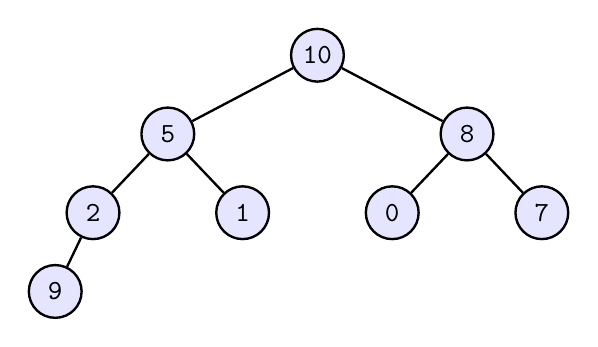
\begin{tikzpicture}

\fill[blue!10] (0.0, 0.0) circle (0.35);
\node [line width=0.03cm,black,minimum size=0.6699999999999999cm,draw,circle] at (0.0,0.0)(10){};\draw (0.0, 0.0) node[color=black] {\texttt{10}};
\fill[blue!10] (-1.9, -1.0) circle (0.35);
\node [line width=0.03cm,black,minimum size=0.6699999999999999cm,draw,circle] at (-1.9,-1.0)(5){};\draw (-1.9, -1.0) node[color=black] {\texttt{5}};
\fill[blue!10] (1.9, -1.0) circle (0.35);
\node [line width=0.03cm,black,minimum size=0.6699999999999999cm,draw,circle] at (1.9,-1.0)(8){};\draw (1.9, -1.0) node[color=black] {\texttt{8}};
\fill[blue!10] (-2.85, -2.0) circle (0.35);
\node [line width=0.03cm,black,minimum size=0.6699999999999999cm,draw,circle] at (-2.85,-2.0)(2){};\draw (-2.85, -2.0) node[color=black] {\texttt{2}};
\fill[blue!10] (-0.95, -2.0) circle (0.35);
\node [line width=0.03cm,black,minimum size=0.6699999999999999cm,draw,circle] at (-0.95,-2.0)(1){};\draw (-0.95, -2.0) node[color=black] {\texttt{1}};
\fill[blue!10] (0.95, -2.0) circle (0.35);
\node [line width=0.03cm,black,minimum size=0.6699999999999999cm,draw,circle] at (0.95,-2.0)(0){};\draw (0.95, -2.0) node[color=black] {\texttt{0}};
\fill[blue!10] (2.85, -2.0) circle (0.35);
\node [line width=0.03cm,black,minimum size=0.6699999999999999cm,draw,circle] at (2.85,-2.0)(7){};\draw (2.85, -2.0) node[color=black] {\texttt{7}};
\fill[blue!10] (-3.33, -3.0) circle (0.35);
\node [line width=0.03cm,black,minimum size=0.6699999999999999cm,draw,circle] at (-3.33,-3.0)(9){};\draw (-3.33, -3.0) node[color=black] {\texttt{9}};\draw[line width=0.03cm,black] (10) to  (5);
\draw[line width=0.03cm,black] (10) to  (8);
\draw[line width=0.03cm,black] (5) to  (2);
\draw[line width=0.03cm,black] (5) to  (1);
\draw[line width=0.03cm,black] (8) to  (0);
\draw[line width=0.03cm,black] (8) to  (7);
\draw[line width=0.03cm,black] (2) to  (9);
\end{tikzpicture}

\end{center}



It's easy to see that in the DFA, the $a$--
and $b$--transitions from the state $\{\}$ goes back to itself.
Therefore the completed DFA is this:


\begin{center}
\begin{tikzpicture}[>=triangle 60,shorten >=0.5pt,node distance=2cm,auto,initial text=, double distance=2pt]
\node[state,initial] (A) at (  0,  0) {$\{q_0\}$};
\node[state] (B) at (  3,  0) {$\{\}$};

\path[->]
(A) edge [bend left=0,pos=0.5,above] node {$a,b$} (B)
(B) edge [loop above] node {$a,b$} ()

;
\end{tikzpicture}
\end{center}
    



\newpage

Solution to Exercise \ref{ex:dfa-as-powerful-as-nfa1}\labeltext{}{sol:dfa-as-powerful-as-nfa1}.

\tinysidebar{\debug{exercises/{dfa-as-powerful-as-nfa1/answer.tex}}}

    Solution not provided.
    

\newpage

Solution to Exercise \ref{ex:dfa-as-powerful-as-nfa2}\labeltext{}{sol:dfa-as-powerful-as-nfa2}.

\tinysidebar{\debug{exercises/{dfa-as-powerful-as-nfa2/answer.tex}}}

    Solution not provided.
    

\newpage

Solution to Exercise \ref{ex:dfa-as-powerful-as-nfa3}\labeltext{}{sol:dfa-as-powerful-as-nfa3}.

\tinysidebar{\debug{exercises/{dfa-as-powerful-as-nfa3/answer.tex}}}

    Solution not provided.
    

\newpage

Solution to Exercise \ref{ex:dfa-as-powerful-as-nfa4}\labeltext{}{sol:dfa-as-powerful-as-nfa4}.

\tinysidebar{\debug{exercises/{dfa-as-powerful-as-nfa4/answer.tex}}}

    Solution not provided.
    

\newpage

Solution to Exercise \ref{ex:closure0}\labeltext{}{sol:closure0}.

\tinysidebar{\debug{exercises/{closure0/answer.tex}}}

    Solution not provided.
    

\newpage

Solution to Exercise \ref{ex:closure1}\labeltext{}{sol:closure1}.

\tinysidebar{\debug{exercises/{closure1/answer.tex}}}

    Solution not provided.
    

\newpage

Solution to Exercise \ref{ex:closure2}\labeltext{}{sol:closure2}.

\tinysidebar{\debug{exercises/{closure2/answer.tex}}}

    Solution not provided.
    

\newpage

Solution to Exercise \ref{ex:closure3}\labeltext{}{sol:closure3}.

\tinysidebar{\debug{exercises/{closure3/answer.tex}}}

    Solution not provided.
    

\newpage

Solution to Exercise \ref{ex:closure4}\labeltext{}{sol:closure4}.

\tinysidebar{\debug{exercises/{closure4/answer.tex}}}

    Solution not provided.
    

\newpage

Solution to Exercise \ref{ex:closure5}\labeltext{}{sol:closure5}.

\tinysidebar{\debug{exercises/{closure5/answer.tex}}}

    Solution not provided.
    

\newpage

Solution to Exercise \ref{ex:closure6}\labeltext{}{sol:closure6}.

\tinysidebar{\debug{exercises/{closure6/answer.tex}}}

    Solution not provided.
    

\newpage

Solution to Exercise \ref{ex:closure7}\labeltext{}{sol:closure7}.

\tinysidebar{\debug{exercises/{closure7/answer.tex}}}

    Solution not provided.
    

\newpage

Solution to Exercise \ref{ex:closure8}\labeltext{}{sol:closure8}.

\tinysidebar{\debug{exercises/{closure8/answer.tex}}}

    Solution not provided.
    

\newpage

Solution to Exercise \ref{ex:closure9}\labeltext{}{sol:closure9}.

\tinysidebar{\debug{exercises/{closure9/answer.tex}}}

    Solution not provided.
    

\newpage

Solution to Exercise \ref{ex:closure10}\labeltext{}{sol:closure10}.

\tinysidebar{\debug{exercises/{closure10/answer.tex}}}

    Solution not provided.
    

\newpage

Solution to Exercise \ref{ex:closure11}\labeltext{}{sol:closure11}.

\tinysidebar{\debug{exercises/{closure11/answer.tex}}}

    Solution not provided.
    

\newpage

Solution to Exercise \ref{ex:closure12}\labeltext{}{sol:closure12}.

\tinysidebar{\debug{exercises/{closure12/answer.tex}}}

    Solution not provided.
    


%\end{comment}

\newpage%-*-latex-*-
\sectionthree{Function call}
\begin{python0}
from solutions import *; clear()
\end{python0}

The runtime analysis for function call is similar when it comes to
computing the runtime of the \textit{body} of the function.
The only other things you need to be careful about are
\begin{enumerate}[nosep]
\item the cost of parameter passing
\item the cost of entering the function
\item the cost of returning from the function
\item the cost of return value
\end{enumerate}
(See CISS360 for details.
Also, see CISS240 note on functions, especially the function call stack.)
Here, cost means both time and memory.
You'll definitely need to know how to compute the cost for the case of
recursive functions.

Suppose you have a function \verb!f()!
that takes an array and returns the first value:
\begin{console}
int f(int x[])
{
    return x[0];
}
\end{console}
and \verb!main()! calls \verb!f()! like this:
\begin{console}
int main()
{
    int x[] = {1, 2, 3};
    // A. start timing
    int y = f(x);
    // B. end timing
    return 0;
}
\end{console}
What is the time taken (from point A to point B)?
Here's roughly what happens:
\begin{tightlist}
\item[1.] The arguments are stored somewhere (for instance in the function call stack). For this example, the address \verb!x! is stored.
\item[2.] The point of return from \verb!f()! is stored somewhere (for instance in the function call stack).
This means the address of the machine code to be executed after returning
is stored.
\item[3.] The \defone{program counter} is set to the address of \verb!f()!.
  The program counter is a device in the CPU that basically remembers
  the address of the machine code of your program to execute next.
\item[4.]
  Function \verb!f()! begins execution including
  creating parameters using the value(s) stored in the
  function call stack.
\item[5.] 
  If there is a return value, the function has to store
  the return value somewhere.
\item[6.]
  The program counter is set to the point of return from
  function call \verb!f()!.
\item[7.]
  \verb!main()! continues execution.
\end{tightlist}
(I said roughly because it's an over-simplification, but sufficient for us to
compute the time and space complexity.)

The time taken to set the program counter in order to enter \verb!f()! or return to
\verb!main()! is constant.
The time taken to store the point of return to \verb!main()! is also constant.
The space usage for address of the function and point of return is also constant.
So we don't really care too much about the above, time-wise or space-wise.
The main cost would be the time and space usage for
\begin{tightlist}
  \li storing the arguments
  \li retrieving the arguments and constructing the parameters
  \li storing return value
\end{tightlist}

In the case of our example
\begin{Verbatim}[frame=single,fontsize=\footnotesize]
int f(int x[])
{
    return x[0];
}
\end{Verbatim}
the argument is the address of an array.
The amount of memory used is constant.
So the time to store the address,
retrieving the address, setting the parameter \verb!x! to this address
are all constant.
\verb!x! is a pointer since, from CISS245, the above code is the same
as
\begin{Verbatim}[frame=single,fontsize=\footnotesize]
int f(int * const x)
{
    return x[0];
}
\end{Verbatim}
so \verb!x! is most likely a 64-bit pointer (or 32).
For sure it does not depend on the size of the array.
So that space complexity is constant too.
No matter how large the array \verb!x! points to, \verb!x! consumes
64 bits.
That's why the time taken to set up \verb!x!
and the space usage of \verb!x! are all constant.
(Don't remember pointers?
You had better re-study your pointer notes from CISS245.)

Therefore the total runtime to execute \verb!f()! is $O(1)$
and the space complexity if also $O(1)$.

Now suppose I want to use a \verb!std::vector< int >! instead of an
integer array.
What will happen then?

If I do this:
\begin{console}
int f(const std::vector< int > & x)
{
    return x[0];
}
\end{console}
then all timing are the same as before except that we need to think about
the time for setting up \verb!x!.
In this case, \verb!x! is a reference, which (recall) is just like a pointer.
So the total runtime is still $O(1)$ and the space complexity is still $O(1)$.

Now come the trick question ... what about this:
\begin{console}
int f(const std::vector< int > x)
{
    return x[0];
}
\end{console}
or
\begin{console}
int f(std::vector< int > x)
{
    return x[0];
}
\end{console}
In this case, \verb!x! is a \verb!std::vector< int >! \textit{object} -- it is
not a reference and not a pointer.
If in \verb!main()!, I have
\begin{console}
int main()
{
    std::vector< int > y;
    ...
    std::cout << f(y) << '\n';
    ...
}
\end{console}
then the \verb!x! of \verb!f()! is a \textit{copy} of \verb!y! of \verb!main()!,
created through the
copy constructor of \verb!std::vector!.
If \verb!y! is a vector of $1000$ values, then it takes
a certain amount of time to set up \verb!x!,
which includes requesting memory for \verb!x! and
\textit{copying} the 1000 values of \verb!y! to \verb!x!.
And if \verb!y! is a vector of $1000000000$ values, then it
takes even more time to set up \verb!x!. 
Therefore the set up time for \verb!x! is actually $O(n)$
where $n$ is the size of \verb!y!.
Hence this algorithm has a total runtime of $O(n)$ and the space complexity is also
$O(n)$.

In the same way if you \textit{return} a value that is large in size, then the time
due to returning might not be $O(1)$.
For instance look at this:
\begin{console}
std::vector< int > f(std::vector< int > & v)
{
    return v;
}
\end{console}
In this case, the parameter set up time is $O(1)$ because \verb!v! is a reference.
But the return type is a \verb!std::vector< int >! value (not reference).
So the copy constructor is used to create a \verb!std::vector< int >! value
for returning
from the value \verb!v! references.
So hidden in the above code is a $O(n)$ runtime where $n$ is the
size of the vector that \verb!v! references
and the space complexity is also $O(n)$.

This explains why in CISS245,
for \lq\lq large" variables such as \verb!struct! variables or objects,
we always pass by pointer or pass by reference.
This is the same reason that an array parameter of a function
is actually a pointer:
\begin{console}
void f(int x[]) // same as void f(int * const x)
{
     ...
     return; 
}
\end{console}



\begin{ex} 
  \label{ex:some-decision1}
  \tinysidebar{\debug{exercises/{empty0/question.tex}}}
  \solutionlink{sol:some-decision1}
  \qed
\end{ex} 
\begin{python0}
from solutions import *
add(label="ex:some-decision1",
    srcfilename='exercises/some-decision1/answer.tex') 
\end{python0}
 


Now suppose you have a sequence of function calls where the first function
called is \verb!f()!:
\begin{Verbatim}[frame=single,fontsize=\footnotesize,numbers=left]
void j(double y)
{
     int c[30];
}
void i(int x[])
{
     int c[30];
}
void h(int x[], double y)
{
     int c[30];
     i(x);
}
double g(int x[])
{
    double y;
    int b[20];
    h(x, y);
    int d[40];
    j(y);
}
int f(int x[])
{
    int a[10];
    g(x)
    return 42;
}
\end{Verbatim}
The following is the function call graph:
%-*-latex-*-
\begin{center}
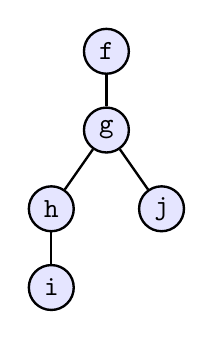
\begin{tikzpicture}

\fill[blue!10] (2.1, 0.0) circle (0.3);
\node [line width=0.03cm,black,minimum size=0.57cm,draw,circle] at (2.1,0.0)(f){};\draw (2.1, 0.0) node[color=black] {\texttt{f}};
\fill[blue!10] (2.1, -1.0) circle (0.3);
\node [line width=0.03cm,black,minimum size=0.57cm,draw,circle] at (2.1,-1.0)(g){};\draw (2.1, -1.0) node[color=black] {\texttt{g}};
\fill[blue!10] (1.4, -2.0) circle (0.3);
\node [line width=0.03cm,black,minimum size=0.57cm,draw,circle] at (1.4,-2.0)(h){};\draw (1.4, -2.0) node[color=black] {\texttt{h}};
\fill[blue!10] (1.4, -3.0) circle (0.3);
\node [line width=0.03cm,black,minimum size=0.57cm,draw,circle] at (1.4,-3.0)(i){};\draw (1.4, -3.0) node[color=black] {\texttt{i}};
\fill[blue!10] (2.8, -2.0) circle (0.3);
\node [line width=0.03cm,black,minimum size=0.57cm,draw,circle] at (2.8,-2.0)(j){};\draw (2.8, -2.0) node[color=black] {\texttt{j}};\draw[line width=0.03cm,black] (f) to  (g);
\draw[line width=0.03cm,black] (g) to  (h);
\draw[line width=0.03cm,black] (g) to  (j);
\draw[line width=0.03cm,black] (h) to  (i);
\end{tikzpicture}

\end{center}


The following lists memory usage (by line numbers) at various points
during the program execution:
\begin{align*}
  \text{end of line 24}&: \text{10 integers} \\
  \text{end of line 17}&: \text{30 integers, 1 pointer, 1 double} \\
  \text{end of line 11}&: \text{60 integers, 2 pointer, 2 double} \\
  \text{end of line 26}&: \text{10 integers}
\end{align*}
Recall (from CISS245) that this structure is called a tree where \verb!f! is called the root
of the tree.
We'll be studying trees in detail.

Note that the space usage grows \textit{and shrinks} with program execution since
\begin{enumerate}[nosep]
  \li
  memory used by a local variable is reclaimed when this local variable
  goes out of scope
  \li
  memory used by a function is reclaimed when you exit a function
  \li 
  memory in the heap is reclaimed when you deallocate the memory
\end{enumerate}
However time usage only increases with program execution.
You can reuse memory, but you cannot reuse time!!!
To compute the worst case scenario of memory usage, i.e., maximum memory usage,
you would need to consider the
memory usage by
\begin{enumerate}[nosep]  
  \li \verb!f()!
  \li \verb!f()! , \verb!g()!, 
  \li \verb!f()! , \verb!g()!, \verb!h()!
  \li \verb!f()!, \verb!g()!, \verb!h()!, \verb!i()! and
  \li \verb!f()!, \verb!g()!, \verb!j()!
\end{enumerate}
in the function call graph:
%-*-latex-*-
\begin{center}
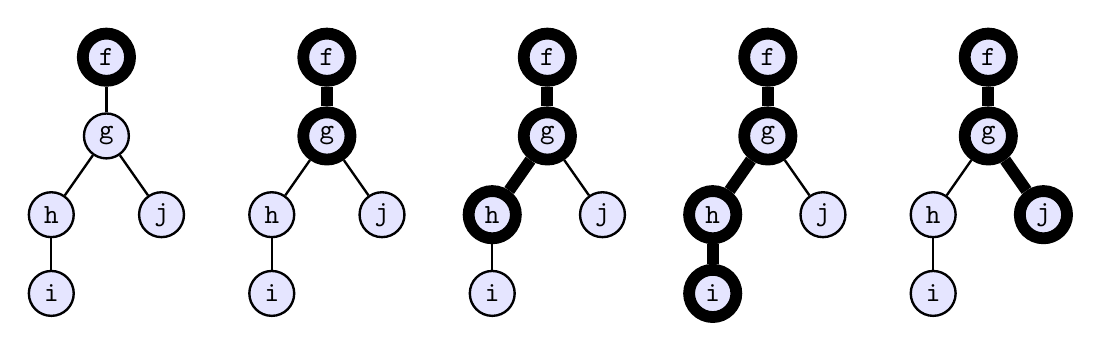
\begin{tikzpicture}

\fill[blue!10] (0.7, 0.0) circle (0.3);
\node [line width=0.15cm,black,minimum size=0.6cm,draw,circle] at (0.7,0.0)(A){};\draw (0.7, 0.0) node[color=black] {\texttt{f}};
\fill[blue!10] (0.7, -1.0) circle (0.3);
\node [line width=0.03cm,black,minimum size=0.57cm,draw,circle] at (0.7,-1.0)(B){};\draw (0.7, -1.0) node[color=black] {\texttt{g}};
\fill[blue!10] (0.0, -2.0) circle (0.3);
\node [line width=0.03cm,black,minimum size=0.57cm,draw,circle] at (0.0,-2.0)(C){};\draw (0.0, -2.0) node[color=black] {\texttt{h}};
\fill[blue!10] (0.0, -3.0) circle (0.3);
\node [line width=0.03cm,black,minimum size=0.57cm,draw,circle] at (0.0,-3.0)(D){};\draw (0.0, -3.0) node[color=black] {\texttt{i}};
\fill[blue!10] (1.4, -2.0) circle (0.3);
\node [line width=0.03cm,black,minimum size=0.57cm,draw,circle] at (1.4,-2.0)(E){};\draw (1.4, -2.0) node[color=black] {\texttt{j}};
\fill[blue!10] (9.1, 0.0) circle (0.3);
\node [line width=0.15cm,black,minimum size=0.6cm,draw,circle] at (9.1,0.0)(f){};\draw (9.1, 0.0) node[color=black] {\texttt{f}};
\fill[blue!10] (9.1, -1.0) circle (0.3);
\node [line width=0.15cm,black,minimum size=0.6cm,draw,circle] at (9.1,-1.0)(g){};\draw (9.1, -1.0) node[color=black] {\texttt{g}};
\fill[blue!10] (8.4, -2.0) circle (0.3);
\node [line width=0.15cm,black,minimum size=0.6cm,draw,circle] at (8.4,-2.0)(h){};\draw (8.4, -2.0) node[color=black] {\texttt{h}};
\fill[blue!10] (8.4, -3.0) circle (0.3);
\node [line width=0.15cm,black,minimum size=0.6cm,draw,circle] at (8.4,-3.0)(i){};\draw (8.4, -3.0) node[color=black] {\texttt{i}};
\fill[blue!10] (9.8, -2.0) circle (0.3);
\node [line width=0.03cm,black,minimum size=0.57cm,draw,circle] at (9.8,-2.0)(j){};\draw (9.8, -2.0) node[color=black] {\texttt{j}};
\fill[blue!10] (11.9, 0.0) circle (0.3);
\node [line width=0.15cm,black,minimum size=0.6cm,draw,circle] at (11.9,0.0)(F){};\draw (11.9, 0.0) node[color=black] {\texttt{f}};
\fill[blue!10] (11.9, -1.0) circle (0.3);
\node [line width=0.15cm,black,minimum size=0.6cm,draw,circle] at (11.9,-1.0)(G){};\draw (11.9, -1.0) node[color=black] {\texttt{g}};
\fill[blue!10] (11.2, -2.0) circle (0.3);
\node [line width=0.03cm,black,minimum size=0.57cm,draw,circle] at (11.2,-2.0)(H){};\draw (11.2, -2.0) node[color=black] {\texttt{h}};
\fill[blue!10] (11.2, -3.0) circle (0.3);
\node [line width=0.03cm,black,minimum size=0.57cm,draw,circle] at (11.2,-3.0)(I){};\draw (11.2, -3.0) node[color=black] {\texttt{i}};
\fill[blue!10] (12.6, -2.0) circle (0.3);
\node [line width=0.15cm,black,minimum size=0.6cm,draw,circle] at (12.6,-2.0)(J){};\draw (12.6, -2.0) node[color=black] {\texttt{j}};
\fill[blue!10] (3.5, 0.0) circle (0.3);
\node [line width=0.15cm,black,minimum size=0.6cm,draw,circle] at (3.5,0.0)(a){};\draw (3.5, 0.0) node[color=black] {\texttt{f}};
\fill[blue!10] (3.5, -1.0) circle (0.3);
\node [line width=0.15cm,black,minimum size=0.6cm,draw,circle] at (3.5,-1.0)(b){};\draw (3.5, -1.0) node[color=black] {\texttt{g}};
\fill[blue!10] (2.8, -2.0) circle (0.3);
\node [line width=0.03cm,black,minimum size=0.57cm,draw,circle] at (2.8,-2.0)(c){};\draw (2.8, -2.0) node[color=black] {\texttt{h}};
\fill[blue!10] (2.8, -3.0) circle (0.3);
\node [line width=0.03cm,black,minimum size=0.57cm,draw,circle] at (2.8,-3.0)(d){};\draw (2.8, -3.0) node[color=black] {\texttt{i}};
\fill[blue!10] (4.2, -2.0) circle (0.3);
\node [line width=0.03cm,black,minimum size=0.57cm,draw,circle] at (4.2,-2.0)(e){};\draw (4.2, -2.0) node[color=black] {\texttt{j}};
\fill[blue!10] (6.3, 0.0) circle (0.3);
\node [line width=0.15cm,black,minimum size=0.6cm,draw,circle] at (6.3,0.0)(V){};\draw (6.3, 0.0) node[color=black] {\texttt{f}};
\fill[blue!10] (6.3, -1.0) circle (0.3);
\node [line width=0.15cm,black,minimum size=0.6cm,draw,circle] at (6.3,-1.0)(W){};\draw (6.3, -1.0) node[color=black] {\texttt{g}};
\fill[blue!10] (5.6, -2.0) circle (0.3);
\node [line width=0.15cm,black,minimum size=0.6cm,draw,circle] at (5.6,-2.0)(X){};\draw (5.6, -2.0) node[color=black] {\texttt{h}};
\fill[blue!10] (5.6, -3.0) circle (0.3);
\node [line width=0.03cm,black,minimum size=0.57cm,draw,circle] at (5.6,-3.0)(Y){};\draw (5.6, -3.0) node[color=black] {\texttt{i}};
\fill[blue!10] (7.0, -2.0) circle (0.3);
\node [line width=0.03cm,black,minimum size=0.57cm,draw,circle] at (7.0,-2.0)(Z){};\draw (7.0, -2.0) node[color=black] {\texttt{j}};\draw[line width=0.03cm,black] (A) to  (B);
\draw[line width=0.03cm,black] (B) to  (C);
\draw[line width=0.03cm,black] (B) to  (E);
\draw[line width=0.03cm,black] (C) to  (D);
\draw[line width=0.15cm,black] (a) to  (b);
\draw[line width=0.03cm,black] (b) to  (c);
\draw[line width=0.03cm,black] (b) to  (e);
\draw[line width=0.03cm,black] (c) to  (d);
\draw[line width=0.15cm,black] (V) to  (W);
\draw[line width=0.15cm,black] (W) to  (X);
\draw[line width=0.03cm,black] (W) to  (Z);
\draw[line width=0.03cm,black] (X) to  (Y);
\draw[line width=0.15cm,black] (f) to  (g);
\draw[line width=0.15cm,black] (g) to  (h);
\draw[line width=0.03cm,black] (g) to  (j);
\draw[line width=0.15cm,black] (h) to  (i);
\draw[line width=0.15cm,black] (F) to  (G);
\draw[line width=0.03cm,black] (G) to  (H);
\draw[line width=0.15cm,black] (G) to  (J);
\draw[line width=0.03cm,black] (H) to  (I);
\end{tikzpicture}

\end{center}


For the case of computing runtime, you have to look at the time used
for \textit{all} functions:
%-*-latex-*-
\begin{center}
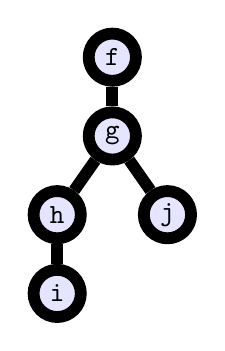
\begin{tikzpicture}

\fill[blue!10] (0.7, 0.0) circle (0.3);
\node [line width=0.15cm,black,minimum size=0.6cm,draw,circle] at (0.7,0.0)(A){};\draw (0.7, 0.0) node[color=black] {\texttt{f}};
\fill[blue!10] (0.7, -1.0) circle (0.3);
\node [line width=0.15cm,black,minimum size=0.6cm,draw,circle] at (0.7,-1.0)(B){};\draw (0.7, -1.0) node[color=black] {\texttt{g}};
\fill[blue!10] (0.0, -2.0) circle (0.3);
\node [line width=0.15cm,black,minimum size=0.6cm,draw,circle] at (0.0,-2.0)(C){};\draw (0.0, -2.0) node[color=black] {\texttt{h}};
\fill[blue!10] (0.0, -3.0) circle (0.3);
\node [line width=0.15cm,black,minimum size=0.6cm,draw,circle] at (0.0,-3.0)(D){};\draw (0.0, -3.0) node[color=black] {\texttt{i}};
\fill[blue!10] (1.4, -2.0) circle (0.3);
\node [line width=0.15cm,black,minimum size=0.6cm,draw,circle] at (1.4,-2.0)(E){};\draw (1.4, -2.0) node[color=black] {\texttt{j}};\draw[line width=0.15cm,black] (A) to  (B);
\draw[line width=0.15cm,black] (B) to  (C);
\draw[line width=0.15cm,black] (B) to  (E);
\draw[line width=0.15cm,black] (C) to  (D);
\end{tikzpicture}

\end{center}


and if \verb!g()! calls either \verb!h()! or \verb!j()! (but not both),
then you have to consider
\begin{enumerate}[nosep]  
  \li \verb!f()!, \verb!g()!, \verb!h()!, \verb!i()! and
  \li \verb!f()!, \verb!g()!, \verb!j()!
\end{enumerate}

Remember: you can reuse space, but you cannot reuse time!!!


\begin{ex} 
  \label{ex:some-decision1}
  \tinysidebar{\debug{exercises/{empty0/question.tex}}}
  \solutionlink{sol:some-decision1}
  \qed
\end{ex} 
\begin{python0}
from solutions import *
add(label="ex:some-decision1",
    srcfilename='exercises/some-decision1/answer.tex') 
\end{python0}


\begin{ex} 
  \label{ex:some-decision1}
  \tinysidebar{\debug{exercises/{empty0/question.tex}}}
  \solutionlink{sol:some-decision1}
  \qed
\end{ex} 
\begin{python0}
from solutions import *
add(label="ex:some-decision1",
    srcfilename='exercises/some-decision1/answer.tex') 
\end{python0}


\begin{ex} 
  \label{ex:some-decision1}
  \tinysidebar{\debug{exercises/{empty0/question.tex}}}
  \solutionlink{sol:some-decision1}
  \qed
\end{ex} 
\begin{python0}
from solutions import *
add(label="ex:some-decision1",
    srcfilename='exercises/some-decision1/answer.tex') 
\end{python0}


%\newpage
%\subsection*{Solutions}
%
\newpage
\section*{Solutions}
Solution to Exercise \ref{ex:dfa0}\labeltext{}{sol:dfa0}.

\tinysidebar{\debug{exercises/{dfa0/answer.tex}}}

    Solution not provided.
    

\newpage

Solution to Exercise \ref{ex:dfa1}\labeltext{}{sol:dfa1}.

\tinysidebar{\debug{exercises/{dfa1/answer.tex}}}
  The ID computation is
  \begin{align*}
    (q_0, aba)
    &\vdash (\delta(q_0, a), ba) = (q_0, ba) \\ 
    &\vdash (\delta(q_0, b), a) = (q_1, a) \\
    &\vdash (\delta(q_1, a), \ep) = (q_0, \ep)
  \end{align*}
  $q_0$ is not an accept state. Therefore $aba$ is not accepted.


\newpage

Solution to Exercise \ref{ex:dfa4}\labeltext{}{sol:dfa4}.

\tinysidebar{\debug{exercises/{dfa4/answer.tex}}}

    Solution not provided.
    

\newpage

Solution to Exercise \ref{ex:dfa5}\labeltext{}{sol:dfa5}.

\tinysidebar{\debug{exercises/{dfa5/answer.tex}}}

    Solution not provided.
    

\newpage

Solution to Exercise \ref{ex:implementing-a-single-dfa0}\labeltext{}{sol:implementing-a-single-dfa0}.

\tinysidebar{\debug{exercises/{implementing-a-single-dfa0/answer.tex}}}

    Solution not provided.
    

\newpage

Solution to Exercise \ref{ex:nfastatediag0}\labeltext{}{sol:nfastatediag0}.

\tinysidebar{\debug{exercises/{nfastatediag0/answer.tex}}}

    Solution not provided.
    

\newpage

Solution to Exercise \ref{ex:nfastatediag1}\labeltext{}{sol:nfastatediag1}.

\tinysidebar{\debug{exercises/{nfastatediag1/answer.tex}}}

    Solution not provided.
    

\newpage

Solution to Exercise \ref{ex:nfastatediag2}\labeltext{}{sol:nfastatediag2}.

\tinysidebar{\debug{exercises/{nfastatediag2/answer.tex}}}

    Solution not provided.
    

\newpage

Solution to Exercise \ref{ex:nfastatediag3}\labeltext{}{sol:nfastatediag3}.

\tinysidebar{\debug{exercises/{nfastatediag3/answer.tex}}}

    Solution not provided.
    

\newpage

Solution to Exercise \ref{ex:nfastatediag4}\labeltext{}{sol:nfastatediag4}.

\tinysidebar{\debug{exercises/{nfastatediag4/answer.tex}}}

    Solution not provided.
    

\newpage

Solution to Exercise \ref{ex:nfastatediag5}\labeltext{}{sol:nfastatediag5}.

\tinysidebar{\debug{exercises/{nfastatediag5/answer.tex}}}

    Solution not provided.
    

\newpage

Solution to Exercise \ref{ex:nfastatediag6}\labeltext{}{sol:nfastatediag6}.

\tinysidebar{\debug{exercises/{nfastatediag6/answer.tex}}}

    Solution not provided.
    

\newpage

Solution to Exercise \ref{ex:nfastatediag7}\labeltext{}{sol:nfastatediag7}.

\tinysidebar{\debug{exercises/{nfastatediag7/answer.tex}}}

    Solution not provided.
    

\newpage

Solution to Exercise \ref{ex:nfastatediag8}\labeltext{}{sol:nfastatediag8}.

\tinysidebar{\debug{exercises/{nfastatediag8/answer.tex}}}

    Solution not provided.
    

\newpage

Solution to Exercise \ref{ex:nfastatediag9}\labeltext{}{sol:nfastatediag9}.

\tinysidebar{\debug{exercises/{nfastatediag9/answer.tex}}}

    Solution not provided.
    

\newpage

Solution to Exercise \ref{ex:nfastatediag10}\labeltext{}{sol:nfastatediag10}.

\tinysidebar{\debug{exercises/{nfastatediag10/answer.tex}}}

    Solution not provided.
    

\newpage

Solution to Exercise \ref{ex:nfastatediag11}\labeltext{}{sol:nfastatediag11}.

\tinysidebar{\debug{exercises/{nfastatediag11/answer.tex}}}

    Solution not provided.
    

\newpage

Solution to Exercise \ref{ex:nfastatediag12}\labeltext{}{sol:nfastatediag12}.

\tinysidebar{\debug{exercises/{nfastatediag12/answer.tex}}}

    Solution not provided.
    

\newpage

Solution to Exercise \ref{ex:nfastatediag13}\labeltext{}{sol:nfastatediag13}.

\tinysidebar{\debug{exercises/{nfastatediag13/answer.tex}}}

    Solution not provided.
    

\newpage

Solution to Exercise \ref{ex:nfa0}\labeltext{}{sol:nfa0}.

\tinysidebar{\debug{exercises/{nfa0/answer.tex}}}
The formal definition of this NFA is $(\Sigma, Q, q_0, \delta, F)$ where
\begin{tightlist}
\li $\Sigma = \{a,b\}$
\li $Q = \{q_0\}$
\li $\delta$ is the function
\[
\delta : Q \times \Sigma_\epsilon \rightarrow P(Q)
\]
given by
\begin{align*}
  \delta(q_0, \epsilon) &= \{\} \\
  \delta(q_0, a) &= \{\} \\
  \delta(q_0, b) &= \{\} 
\end{align*}
\end{tightlist}


\newpage

Solution to Exercise \ref{ex:nfa1}\labeltext{}{sol:nfa1}.

\tinysidebar{\debug{exercises/{nfa1/answer.tex}}}

    Solution not provided.
    

\newpage

Solution to Exercise \ref{ex:nfa2}\labeltext{}{sol:nfa2}.

\tinysidebar{\debug{exercises/{nfa2/answer.tex}}}

    Solution not provided.
    

\newpage

Solution to Exercise \ref{ex:nfa3}\labeltext{}{sol:nfa3}.

\tinysidebar{\debug{exercises/{nfa3/answer.tex}}}

    Solution not provided.
    

\newpage

Solution to Exercise \ref{ex:nfa4}\labeltext{}{sol:nfa4}.

\tinysidebar{\debug{exercises/{nfa4/answer.tex}}}

    Solution not provided.
    

\newpage

Solution to Exercise \ref{ex:nfa5}\labeltext{}{sol:nfa5}.

\tinysidebar{\debug{exercises/{nfa5/answer.tex}}}

    Solution not provided.
    

\newpage

Solution to Exercise \ref{ex:dfa-as-powerful-as-nfa0}\labeltext{}{sol:dfa-as-powerful-as-nfa0}.

\tinysidebar{\debug{exercises/{dfa-as-powerful-as-nfa0/answer.tex}}}
Here's the solution.
Let $\delta$ denote the transition function of $N$.
Note that 
\begin{align*}
  \delta(q_0, \epsilon) = \{\} \\
  \delta(q_0, a) = \{\} \\
  \delta(q_0, b) = \{\} 
\end{align*}
First of all the states are labeled as all the subsets of $\{q_0\}$.


\begin{center}
\begin{tikzpicture}[>=triangle 60,shorten >=0.5pt,node distance=2cm,auto,initial text=, double distance=2pt]
\node[state] (A) at (  0,  0) {$\{q_0\}$};
\node[state] (B) at (  3,  0) {$\{\}$};

\path[->]

;
\end{tikzpicture}
\end{center}
    


The start state is the $\epsilon$-closure of $\{q_0\}$.
However in $N$, there are no $\epsilon$--transitions out of 
$q_0$.
So the $\epsilon$-closure of $\{q_0\}$ is in fact $\{q_0\}$, i.e.
$\overline{\{q_0\}} = \{q_0\}$
The $\DFA$ is now this:


\begin{longtable}{|r||r|r|r|r|r|}
\hline 
         & $w_1$ & $w_2$ & $w_3$ & $w_4$ & $\ldots$ \\ \hline \hline 
$M_1$    &       &       &       &       &          \\ \hline 
$M_2$    &       &       &       &       &          \\ \hline 
$M_3$    &       &       &       &       &          \\ \hline 
$M_4$    &       &       &       &       &          \\ \hline 
$\ldots$ &       &       &       &       &          \\ \hline 
\end{longtable}
        


Now I will compute the $a$--transition of the state $\{q_0\}$.
Let $\delta^\DFA$ denote the transition function of the $\DFA$
that we're building.
Then
\begin{align*}
\delta( \{q_0, a\} ) 
&= \overline{ \bigcup_{q \in \{q_0\}} \delta(q, a)} \\
&= \overline{ \delta(q_0, a) } \\
&= \overline{ \emptyset } \\
&= \emptyset
\end{align*}
The (incomplete) $\DFA$ now looks like this:


\begin{longtable}{|r||r|r|r|r|r|}
\hline 
         & $w_1$ & $w_2$ & $w_3$ & $w_4$ & $\ldots$ \\ \hline \hline 
$M_1$    & 0     & 0     & 1     & 0     & ...      \\ \hline 
$M_2$    & 1     & 0     & 1     & 1     & ...      \\ \hline 
$M_3$    & 0     & 1     & 1     & 1     & ...      \\ \hline 
$M_4$    & 1     & 0     & 1     & 1     & ...      \\ \hline 
$\ldots$ &       &       &       &       &          \\ \hline 
\end{longtable}
        


Using the same reasoning we have

\begin{center}
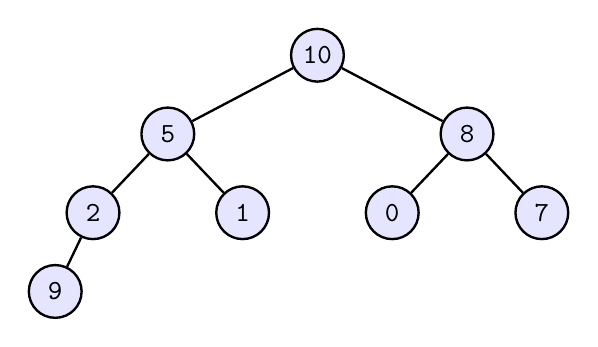
\begin{tikzpicture}

\fill[blue!10] (0.0, 0.0) circle (0.35);
\node [line width=0.03cm,black,minimum size=0.6699999999999999cm,draw,circle] at (0.0,0.0)(10){};\draw (0.0, 0.0) node[color=black] {\texttt{10}};
\fill[blue!10] (-1.9, -1.0) circle (0.35);
\node [line width=0.03cm,black,minimum size=0.6699999999999999cm,draw,circle] at (-1.9,-1.0)(5){};\draw (-1.9, -1.0) node[color=black] {\texttt{5}};
\fill[blue!10] (1.9, -1.0) circle (0.35);
\node [line width=0.03cm,black,minimum size=0.6699999999999999cm,draw,circle] at (1.9,-1.0)(8){};\draw (1.9, -1.0) node[color=black] {\texttt{8}};
\fill[blue!10] (-2.85, -2.0) circle (0.35);
\node [line width=0.03cm,black,minimum size=0.6699999999999999cm,draw,circle] at (-2.85,-2.0)(2){};\draw (-2.85, -2.0) node[color=black] {\texttt{2}};
\fill[blue!10] (-0.95, -2.0) circle (0.35);
\node [line width=0.03cm,black,minimum size=0.6699999999999999cm,draw,circle] at (-0.95,-2.0)(1){};\draw (-0.95, -2.0) node[color=black] {\texttt{1}};
\fill[blue!10] (0.95, -2.0) circle (0.35);
\node [line width=0.03cm,black,minimum size=0.6699999999999999cm,draw,circle] at (0.95,-2.0)(0){};\draw (0.95, -2.0) node[color=black] {\texttt{0}};
\fill[blue!10] (2.85, -2.0) circle (0.35);
\node [line width=0.03cm,black,minimum size=0.6699999999999999cm,draw,circle] at (2.85,-2.0)(7){};\draw (2.85, -2.0) node[color=black] {\texttt{7}};
\fill[blue!10] (-3.33, -3.0) circle (0.35);
\node [line width=0.03cm,black,minimum size=0.6699999999999999cm,draw,circle] at (-3.33,-3.0)(9){};\draw (-3.33, -3.0) node[color=black] {\texttt{9}};\draw[line width=0.03cm,black] (10) to  (5);
\draw[line width=0.03cm,black] (10) to  (8);
\draw[line width=0.03cm,black] (5) to  (2);
\draw[line width=0.03cm,black] (5) to  (1);
\draw[line width=0.03cm,black] (8) to  (0);
\draw[line width=0.03cm,black] (8) to  (7);
\draw[line width=0.03cm,black] (2) to  (9);
\end{tikzpicture}

\end{center}



It's easy to see that in the DFA, the $a$--
and $b$--transitions from the state $\{\}$ goes back to itself.
Therefore the completed DFA is this:


\begin{center}
\begin{tikzpicture}[>=triangle 60,shorten >=0.5pt,node distance=2cm,auto,initial text=, double distance=2pt]
\node[state,initial] (A) at (  0,  0) {$\{q_0\}$};
\node[state] (B) at (  3,  0) {$\{\}$};

\path[->]
(A) edge [bend left=0,pos=0.5,above] node {$a,b$} (B)
(B) edge [loop above] node {$a,b$} ()

;
\end{tikzpicture}
\end{center}
    



\newpage

Solution to Exercise \ref{ex:dfa-as-powerful-as-nfa1}\labeltext{}{sol:dfa-as-powerful-as-nfa1}.

\tinysidebar{\debug{exercises/{dfa-as-powerful-as-nfa1/answer.tex}}}

    Solution not provided.
    

\newpage

Solution to Exercise \ref{ex:dfa-as-powerful-as-nfa2}\labeltext{}{sol:dfa-as-powerful-as-nfa2}.

\tinysidebar{\debug{exercises/{dfa-as-powerful-as-nfa2/answer.tex}}}

    Solution not provided.
    

\newpage

Solution to Exercise \ref{ex:dfa-as-powerful-as-nfa3}\labeltext{}{sol:dfa-as-powerful-as-nfa3}.

\tinysidebar{\debug{exercises/{dfa-as-powerful-as-nfa3/answer.tex}}}

    Solution not provided.
    

\newpage

Solution to Exercise \ref{ex:dfa-as-powerful-as-nfa4}\labeltext{}{sol:dfa-as-powerful-as-nfa4}.

\tinysidebar{\debug{exercises/{dfa-as-powerful-as-nfa4/answer.tex}}}

    Solution not provided.
    

\newpage

Solution to Exercise \ref{ex:closure0}\labeltext{}{sol:closure0}.

\tinysidebar{\debug{exercises/{closure0/answer.tex}}}

    Solution not provided.
    

\newpage

Solution to Exercise \ref{ex:closure1}\labeltext{}{sol:closure1}.

\tinysidebar{\debug{exercises/{closure1/answer.tex}}}

    Solution not provided.
    

\newpage

Solution to Exercise \ref{ex:closure2}\labeltext{}{sol:closure2}.

\tinysidebar{\debug{exercises/{closure2/answer.tex}}}

    Solution not provided.
    

\newpage

Solution to Exercise \ref{ex:closure3}\labeltext{}{sol:closure3}.

\tinysidebar{\debug{exercises/{closure3/answer.tex}}}

    Solution not provided.
    

\newpage

Solution to Exercise \ref{ex:closure4}\labeltext{}{sol:closure4}.

\tinysidebar{\debug{exercises/{closure4/answer.tex}}}

    Solution not provided.
    

\newpage

Solution to Exercise \ref{ex:closure5}\labeltext{}{sol:closure5}.

\tinysidebar{\debug{exercises/{closure5/answer.tex}}}

    Solution not provided.
    

\newpage

Solution to Exercise \ref{ex:closure6}\labeltext{}{sol:closure6}.

\tinysidebar{\debug{exercises/{closure6/answer.tex}}}

    Solution not provided.
    

\newpage

Solution to Exercise \ref{ex:closure7}\labeltext{}{sol:closure7}.

\tinysidebar{\debug{exercises/{closure7/answer.tex}}}

    Solution not provided.
    

\newpage

Solution to Exercise \ref{ex:closure8}\labeltext{}{sol:closure8}.

\tinysidebar{\debug{exercises/{closure8/answer.tex}}}

    Solution not provided.
    

\newpage

Solution to Exercise \ref{ex:closure9}\labeltext{}{sol:closure9}.

\tinysidebar{\debug{exercises/{closure9/answer.tex}}}

    Solution not provided.
    

\newpage

Solution to Exercise \ref{ex:closure10}\labeltext{}{sol:closure10}.

\tinysidebar{\debug{exercises/{closure10/answer.tex}}}

    Solution not provided.
    

\newpage

Solution to Exercise \ref{ex:closure11}\labeltext{}{sol:closure11}.

\tinysidebar{\debug{exercises/{closure11/answer.tex}}}

    Solution not provided.
    

\newpage

Solution to Exercise \ref{ex:closure12}\labeltext{}{sol:closure12}.

\tinysidebar{\debug{exercises/{closure12/answer.tex}}}

    Solution not provided.
    


\newpage%-*-latex-*-
\sectionthree{Recursive function call}
\begin{python0}
from solutions import *; clear()
\end{python0}

Now let me consider the case of recursive functions.
Recursive functions can take many forms.
I'll focus on three typical cases.

Of course we have to look at Fibonacci:
\begin{Verbatim}[frame=single,fontsize=\footnotesize]
int fib(int n)
{
    if (n == 0 || n == 1)
    {
        return 1;
    }
    else
    {
        return fib(n - 1) + fib(n - 2);
    }
}
\end{Verbatim}
In this case
\[
\texttt{fib(n)} \text{ calls \texttt{fib(n - 1)}, \texttt{fib(n - 2)} \text{ and performs some computation}} 
\]
In general a recurrence that looks like
\[
\texttt{f(n)} \text{ calls \texttt{f(n - 1)} \text{ and performs some computation}} 
\]
or
\[
\texttt{f(n)} \text{ calls } \texttt{f(n - 1)}, \texttt{f(n - 2)} \text{ and performs some computation} 
\]
or
\[
\texttt{f(n)} \text{ calls } \texttt{f(n - 1)}, \texttt{f(n - 2)}, \texttt{f(n - 3)} \text{ and performs some computation} 
\]
or
\[
\texttt{f(n)} \text{ calls } \texttt{f(n - 2)}, ... , \texttt{f(n - 5)} \text{ and performs some computation} 
\]
etc.~are called \defone{linear recursion}.

Here's the function call graph for \verb!fib(4)!:
\input{function_call_4.tex}
First let's think about the runtime.
Watchout:
for this section, the \lq\lq runtime of \verb!f(n)!"
refers to the time spent in \verb!f()! and \textit{does not} include
the runtime of the recursive 
\verb!f(n - 1)! and \verb!f(n - 2)!.
For the \textit{next} section,
the \lq\lq runtime of \verb!f(n)!" \textit{will} include
the runtime of the recursive function calls
\verb!f(n - 1)! and \verb!f(n - 2)!.
The second method is more common since there are mathematical techniques
to handle runtime computations for the second method.

Each \verb!f(n)! takes constant time, whether it's the
recursive case or the base cases.
Remember I'm not including the time used in recursive function calls.
Let $A$ be the maximum time of \verb!f(n)!
(i.e., maximum of the time for recursive case and the base cases).
Therefore the total time taken of \verb!f(4)! is
$\text{(the number of function calls)} \times A$.
We're tempted to simplify the counting by adding some rectangles
like this:
%-*-latex-*-
\begin{center}
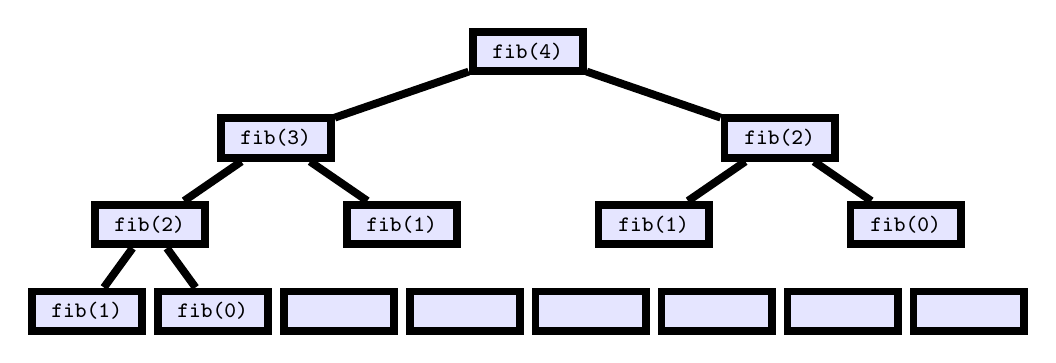
\begin{tikzpicture}

\draw (6.3500000000000005, 0.3)
  node[fill=blue!10,rounded corners=0cm,inner sep=0cm] {

\begin{minipage}[t][0.5cm]{1.4cm}
\mbox{}

\end{minipage}

};
\draw (6.3500000000000005, 0.3)
  node[draw, line width=0.1cm, , color=black,
       rounded corners=0cm, inner sep=0cm,
       name=A] {

\begin{minipage}[t][0.5cm]{1.4cm}
\mbox{}

\end{minipage}

};\draw (6.3500000000000005, 0.3) node[color=black] {\texttt{{\footnotesize \texttt{fib(4)}}}};
\draw (3.1500000000000004, -0.8)
  node[fill=blue!10,rounded corners=0cm,inner sep=0cm] {

\begin{minipage}[t][0.5cm]{1.4cm}
\mbox{}

\end{minipage}

};
\draw (3.1500000000000004, -0.8)
  node[draw, line width=0.1cm, , color=black,
       rounded corners=0cm, inner sep=0cm,
       name=B] {

\begin{minipage}[t][0.5cm]{1.4cm}
\mbox{}

\end{minipage}

};\draw (3.1500000000000004, -0.8) node[color=black] {\texttt{{\footnotesize \texttt{fib(3)}}}};
\draw (9.55, -0.8)
  node[fill=blue!10,rounded corners=0cm,inner sep=0cm] {

\begin{minipage}[t][0.5cm]{1.4cm}
\mbox{}

\end{minipage}

};
\draw (9.55, -0.8)
  node[draw, line width=0.1cm, , color=black,
       rounded corners=0cm, inner sep=0cm,
       name=I] {

\begin{minipage}[t][0.5cm]{1.4cm}
\mbox{}

\end{minipage}

};\draw (9.55, -0.8) node[color=black] {\texttt{{\footnotesize \texttt{fib(2)}}}};
\draw (1.5499999999999998, -1.9000000000000001)
  node[fill=blue!10,rounded corners=0cm,inner sep=0cm] {

\begin{minipage}[t][0.5cm]{1.4cm}
\mbox{}

\end{minipage}

};
\draw (1.5499999999999998, -1.9000000000000001)
  node[draw, line width=0.1cm, , color=black,
       rounded corners=0cm, inner sep=0cm,
       name=C] {

\begin{minipage}[t][0.5cm]{1.4cm}
\mbox{}

\end{minipage}

};\draw (1.5499999999999998, -1.9000000000000001) node[color=black] {\texttt{{\footnotesize \texttt{fib(2)}}}};
\draw (4.75, -1.9000000000000001)
  node[fill=blue!10,rounded corners=0cm,inner sep=0cm] {

\begin{minipage}[t][0.5cm]{1.4cm}
\mbox{}

\end{minipage}

};
\draw (4.75, -1.9000000000000001)
  node[draw, line width=0.1cm, , color=black,
       rounded corners=0cm, inner sep=0cm,
       name=F] {

\begin{minipage}[t][0.5cm]{1.4cm}
\mbox{}

\end{minipage}

};\draw (4.75, -1.9000000000000001) node[color=black] {\texttt{{\footnotesize \texttt{fib(1)}}}};
\draw (7.949999999999999, -1.9000000000000001)
  node[fill=blue!10,rounded corners=0cm,inner sep=0cm] {

\begin{minipage}[t][0.5cm]{1.4cm}
\mbox{}

\end{minipage}

};
\draw (7.949999999999999, -1.9000000000000001)
  node[draw, line width=0.1cm, , color=black,
       rounded corners=0cm, inner sep=0cm,
       name=G] {

\begin{minipage}[t][0.5cm]{1.4cm}
\mbox{}

\end{minipage}

};\draw (7.949999999999999, -1.9000000000000001) node[color=black] {\texttt{{\footnotesize \texttt{fib(1)}}}};
\draw (11.15, -1.9000000000000001)
  node[fill=blue!10,rounded corners=0cm,inner sep=0cm] {

\begin{minipage}[t][0.5cm]{1.4cm}
\mbox{}

\end{minipage}

};
\draw (11.15, -1.9000000000000001)
  node[draw, line width=0.1cm, , color=black,
       rounded corners=0cm, inner sep=0cm,
       name=H] {

\begin{minipage}[t][0.5cm]{1.4cm}
\mbox{}

\end{minipage}

};\draw (11.15, -1.9000000000000001) node[color=black] {\texttt{{\footnotesize \texttt{fib(0)}}}};
\draw (0.75, -3.0)
  node[fill=blue!10,rounded corners=0cm,inner sep=0cm] {

\begin{minipage}[t][0.5cm]{1.4cm}
\mbox{}

\end{minipage}

};
\draw (0.75, -3.0)
  node[draw, line width=0.1cm, , color=black,
       rounded corners=0cm, inner sep=0cm,
       name=D] {

\begin{minipage}[t][0.5cm]{1.4cm}
\mbox{}

\end{minipage}

};\draw (0.75, -3.0) node[color=black] {\texttt{{\footnotesize \texttt{fib(1)}}}};
\draw (2.35, -3.0)
  node[fill=blue!10,rounded corners=0cm,inner sep=0cm] {

\begin{minipage}[t][0.5cm]{1.4cm}
\mbox{}

\end{minipage}

};
\draw (2.35, -3.0)
  node[draw, line width=0.1cm, , color=black,
       rounded corners=0cm, inner sep=0cm,
       name=E] {

\begin{minipage}[t][0.5cm]{1.4cm}
\mbox{}

\end{minipage}

};\draw (2.35, -3.0) node[color=black] {\texttt{{\footnotesize \texttt{fib(0)}}}};
\draw (3.95, -3.0)
  node[fill=blue!10,rounded corners=0cm,inner sep=0cm] {

\begin{minipage}[t][0.5cm]{1.4cm}
\mbox{}

\end{minipage}

};
\draw (3.95, -3.0)
  node[draw, line width=0.1cm, , color=black,
       rounded corners=0cm, inner sep=0cm,
       name=J] {

\begin{minipage}[t][0.5cm]{1.4cm}
\mbox{}

\end{minipage}

};\draw (3.95, -3.0) node[color=black] {\texttt{{\footnotesize \texttt{}}}};
\draw (5.550000000000001, -3.0)
  node[fill=blue!10,rounded corners=0cm,inner sep=0cm] {

\begin{minipage}[t][0.5cm]{1.4cm}
\mbox{}

\end{minipage}

};
\draw (5.550000000000001, -3.0)
  node[draw, line width=0.1cm, , color=black,
       rounded corners=0cm, inner sep=0cm,
       name=K] {

\begin{minipage}[t][0.5cm]{1.4cm}
\mbox{}

\end{minipage}

};\draw (5.550000000000001, -3.0) node[color=black] {\texttt{{\footnotesize \texttt{}}}};
\draw (7.15, -3.0)
  node[fill=blue!10,rounded corners=0cm,inner sep=0cm] {

\begin{minipage}[t][0.5cm]{1.4cm}
\mbox{}

\end{minipage}

};
\draw (7.15, -3.0)
  node[draw, line width=0.1cm, , color=black,
       rounded corners=0cm, inner sep=0cm,
       name=L] {

\begin{minipage}[t][0.5cm]{1.4cm}
\mbox{}

\end{minipage}

};\draw (7.15, -3.0) node[color=black] {\texttt{{\footnotesize \texttt{}}}};
\draw (8.75, -3.0)
  node[fill=blue!10,rounded corners=0cm,inner sep=0cm] {

\begin{minipage}[t][0.5cm]{1.4cm}
\mbox{}

\end{minipage}

};
\draw (8.75, -3.0)
  node[draw, line width=0.1cm, , color=black,
       rounded corners=0cm, inner sep=0cm,
       name=M] {

\begin{minipage}[t][0.5cm]{1.4cm}
\mbox{}

\end{minipage}

};\draw (8.75, -3.0) node[color=black] {\texttt{{\footnotesize \texttt{}}}};
\draw (10.350000000000001, -3.0)
  node[fill=blue!10,rounded corners=0cm,inner sep=0cm] {

\begin{minipage}[t][0.5cm]{1.4cm}
\mbox{}

\end{minipage}

};
\draw (10.350000000000001, -3.0)
  node[draw, line width=0.1cm, , color=black,
       rounded corners=0cm, inner sep=0cm,
       name=N] {

\begin{minipage}[t][0.5cm]{1.4cm}
\mbox{}

\end{minipage}

};\draw (10.350000000000001, -3.0) node[color=black] {\texttt{{\footnotesize \texttt{}}}};
\draw (11.950000000000001, -3.0)
  node[fill=blue!10,rounded corners=0cm,inner sep=0cm] {

\begin{minipage}[t][0.5cm]{1.4cm}
\mbox{}

\end{minipage}

};
\draw (11.950000000000001, -3.0)
  node[draw, line width=0.1cm, , color=black,
       rounded corners=0cm, inner sep=0cm,
       name=O] {

\begin{minipage}[t][0.5cm]{1.4cm}
\mbox{}

\end{minipage}

};\draw (11.950000000000001, -3.0) node[color=black] {\texttt{{\footnotesize \texttt{}}}};\draw[line width=0.1cm,black] (A) to  (B);
\draw[line width=0.1cm,black] (A) to  (I);
\draw[line width=0.1cm,black] (B) to  (C);
\draw[line width=0.1cm,black] (B) to  (F);
\draw[line width=0.1cm,black] (C) to  (D);
\draw[line width=0.1cm,black] (C) to  (E);
\draw[line width=0.1cm,black] (I) to  (G);
\draw[line width=0.1cm,black] (I) to  (H);
\end{tikzpicture}

\end{center}


In this case, the time taken is $\leq (1 + 2 + 2^2 + 2^3) \times A = (2^4 - 1)A$.
For \verb!f(n)!, the time taken is $\leq (2^n - 1)A$, i.e.,
the runtime of the above algorithm is
\[
T(n) = O(2^n)
\]
But is this a tight asymptotic upper bound?
In the next section I'll show you more precisely that the runtime is
\[
T(n) = O(\phi^n)
\]
where $\phi = (1 + \sqrt{5})/2 = 1.6180...$ is the so--called
\defone{golden ratio}.
Note that if $c < 2$, then $c^n$ is asymptotically strictly smaller than $2^n$,
i.e., $c^n = O(2^n)$ but $2^n \neq O(c^n)$.

As for the space complexity,
each \verb!f(n)! takes constant time,
whether the recursive case or base case was executed.
Let $A$ be the maximum space usage of \verb!f(n)!.
Note that $A$ is constant and does not depend on \verb!n!.
It's then clear that the space complexity is due to the
\textit{longest} path in the tree starting from the root:
%-*-latex-*-
\begin{center}
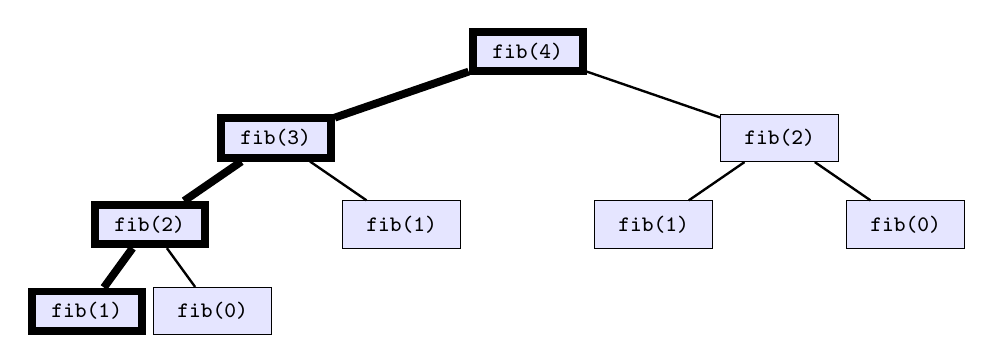
\begin{tikzpicture}

\draw (6.3500000000000005, 0.3)
  node[fill=blue!10,rounded corners=0cm,inner sep=0cm] {

\begin{minipage}[t][0.5cm]{1.4cm}
\mbox{}

\end{minipage}

};
\draw (6.3500000000000005, 0.3)
  node[draw, line width=0.1cm, , color=black,
       rounded corners=0cm, inner sep=0cm,
       name=A] {

\begin{minipage}[t][0.5cm]{1.4cm}
\mbox{}

\end{minipage}

};\draw (6.3500000000000005, 0.3) node[color=black] {\texttt{{\footnotesize \texttt{fib(4)}}}};
\draw (3.1500000000000004, -0.8)
  node[fill=blue!10,rounded corners=0cm,inner sep=0cm] {

\begin{minipage}[t][0.5cm]{1.4cm}
\mbox{}

\end{minipage}

};
\draw (3.1500000000000004, -0.8)
  node[draw, line width=0.1cm, , color=black,
       rounded corners=0cm, inner sep=0cm,
       name=B] {

\begin{minipage}[t][0.5cm]{1.4cm}
\mbox{}

\end{minipage}

};\draw (3.1500000000000004, -0.8) node[color=black] {\texttt{{\footnotesize \texttt{fib(3)}}}};
\draw (9.55, -0.8)
  node[fill=blue!10,rounded corners=0cm,inner sep=0cm] {

\begin{minipage}[t][0.6cm]{1.5cm}
\mbox{}

\end{minipage}

};
\draw (9.55, -0.8)
  node[draw, , , color=black,
       rounded corners=0cm, inner sep=0cm,
       name=I] {

\begin{minipage}[t][0.6cm]{1.5cm}
\mbox{}

\end{minipage}

};\draw (9.55, -0.8) node[color=black] {\texttt{{\footnotesize \texttt{fib(2)}}}};
\draw (1.5499999999999998, -1.9000000000000001)
  node[fill=blue!10,rounded corners=0cm,inner sep=0cm] {

\begin{minipage}[t][0.5cm]{1.4cm}
\mbox{}

\end{minipage}

};
\draw (1.5499999999999998, -1.9000000000000001)
  node[draw, line width=0.1cm, , color=black,
       rounded corners=0cm, inner sep=0cm,
       name=C] {

\begin{minipage}[t][0.5cm]{1.4cm}
\mbox{}

\end{minipage}

};\draw (1.5499999999999998, -1.9000000000000001) node[color=black] {\texttt{{\footnotesize \texttt{fib(2)}}}};
\draw (4.75, -1.9000000000000001)
  node[fill=blue!10,rounded corners=0cm,inner sep=0cm] {

\begin{minipage}[t][0.6cm]{1.5cm}
\mbox{}

\end{minipage}

};
\draw (4.75, -1.9000000000000001)
  node[draw, , , color=black,
       rounded corners=0cm, inner sep=0cm,
       name=F] {

\begin{minipage}[t][0.6cm]{1.5cm}
\mbox{}

\end{minipage}

};\draw (4.75, -1.9000000000000001) node[color=black] {\texttt{{\footnotesize \texttt{fib(1)}}}};
\draw (7.949999999999999, -1.9000000000000001)
  node[fill=blue!10,rounded corners=0cm,inner sep=0cm] {

\begin{minipage}[t][0.6cm]{1.5cm}
\mbox{}

\end{minipage}

};
\draw (7.949999999999999, -1.9000000000000001)
  node[draw, , , color=black,
       rounded corners=0cm, inner sep=0cm,
       name=G] {

\begin{minipage}[t][0.6cm]{1.5cm}
\mbox{}

\end{minipage}

};\draw (7.949999999999999, -1.9000000000000001) node[color=black] {\texttt{{\footnotesize \texttt{fib(1)}}}};
\draw (11.15, -1.9000000000000001)
  node[fill=blue!10,rounded corners=0cm,inner sep=0cm] {

\begin{minipage}[t][0.6cm]{1.5cm}
\mbox{}

\end{minipage}

};
\draw (11.15, -1.9000000000000001)
  node[draw, , , color=black,
       rounded corners=0cm, inner sep=0cm,
       name=H] {

\begin{minipage}[t][0.6cm]{1.5cm}
\mbox{}

\end{minipage}

};\draw (11.15, -1.9000000000000001) node[color=black] {\texttt{{\footnotesize \texttt{fib(0)}}}};
\draw (0.75, -3.0)
  node[fill=blue!10,rounded corners=0cm,inner sep=0cm] {

\begin{minipage}[t][0.5cm]{1.4cm}
\mbox{}

\end{minipage}

};
\draw (0.75, -3.0)
  node[draw, line width=0.1cm, , color=black,
       rounded corners=0cm, inner sep=0cm,
       name=D] {

\begin{minipage}[t][0.5cm]{1.4cm}
\mbox{}

\end{minipage}

};\draw (0.75, -3.0) node[color=black] {\texttt{{\footnotesize \texttt{fib(1)}}}};
\draw (2.35, -3.0)
  node[fill=blue!10,rounded corners=0cm,inner sep=0cm] {

\begin{minipage}[t][0.6cm]{1.5cm}
\mbox{}

\end{minipage}

};
\draw (2.35, -3.0)
  node[draw, , , color=black,
       rounded corners=0cm, inner sep=0cm,
       name=E] {

\begin{minipage}[t][0.6cm]{1.5cm}
\mbox{}

\end{minipage}

};\draw (2.35, -3.0) node[color=black] {\texttt{{\footnotesize \texttt{fib(0)}}}};\draw[line width=0.1cm,black] (A) to  (B);
\draw[line width=0.03cm,black] (A) to  (I);
\draw[line width=0.1cm,black] (B) to  (C);
\draw[line width=0.03cm,black] (B) to  (F);
\draw[line width=0.1cm,black] (C) to  (D);
\draw[line width=0.03cm,black] (C) to  (E);
\draw[line width=0.03cm,black] (I) to  (G);
\draw[line width=0.03cm,black] (I) to  (H);
\end{tikzpicture}

\end{center}


i.e., it's $4A$.
In general, the space complexity of \verb!f(n)! is
\[
\mathsc{Space}(n) = O(n)
\]


\begin{ex} 
  \label{ex:some-decision1}
  \tinysidebar{\debug{exercises/{empty0/question.tex}}}
  \solutionlink{sol:some-decision1}
  \qed
\end{ex} 
\begin{python0}
from solutions import *
add(label="ex:some-decision1",
    srcfilename='exercises/some-decision1/answer.tex') 
\end{python0}



\newpage%-*-latex-*-
\sectionthree{Linear Recursion}
\begin{python0}
from solutions import *; clear()
\end{python0}

Recall that a recursive function is a function that calls itself.
For instance here's Fibonacci again:
{\small
\begin{Verbatim}[frame=single,fontsize=\footnotesize]
def fib(n):
    if n == 0 or n == 1:
        return 1
    else:
        return fib(n - 1) + fib(n - 2)
\end{Verbatim}
}
Or in C/C++:
{\small
\begin{Verbatim}[frame=single,fontsize=\footnotesize]
int fib(int n)
{
    if (n == 0 || n == 1):
        return 1;
    else
        return fib(n - 1) + fib(n - 2);
}
\end{Verbatim}
}
Of course this is your standard first Fibonacci implementation. 
(Review your recursion notes from CISS245.)

The form of this function is derived from math.
In your math classes, one would write this function as
\[
f(n) = 
\begin{cases}
1                   & \text{if $n = 0, 1$} \\
f(n - 1) + f(n - 2) & \text{otherwise}
\end{cases}
\] 
In math, one would also say that this definition is piecewise ... 
because there are two pieces in the definition, right?

Each of the following cases
\[
f(0) = 1, \,\,\,\,\, f(1) = 1
\]
is usually called a \defone{base case}.
The case that has recursion
\[
f(n) = f(n - 1) + f(n - 2) , \,\,\,\,\, n > 1
\]
is called the \defone{recursive case} (duh).

How do you analyze the runtime of the above recursive function?
There are many types of recursion.
The above recursion
\[
f(n) = f(n - 1) + f(n - 2)
\]
is an example of a \defone{linear recursion} with fixed degree.
In the Fibonacci case, the \defone{degree} is 2 because
the parameters in the above are
\[
n, \,\,\,\,\, n - 1, \,\,\,\,\, n - 2
\]
and the largest difference between $n$ and the other parameters is $2$.
In general a degree 2 linear recurrrence $g(n)$ looks like this:
\[
g(n) = a \cdot g(n-1) + b \cdot g(n-2)
\]
where $a,b$ are constants.
A degree 3 linear recurrrence $h(n)$ looks like this:
\[
h(n) = a \cdot h(n-1) + b \cdot h(n-2) + c \cdot h(n-3)
\]
where $a,b,c$ are constants.



Here's what you do.
First you let 
\[
T(n)
\]
denote the total time to execute \verb!f(n)!
\textit{including} the time due to the recursive calls.
That includes the function call, the execution of the body (which can
include the time to execute the base case code or
the time due to the execution of the recursive calls)
and the return.

\begin{Verbatim}[frame=single,fontsize=\footnotesize]
def f(n):                                 t1
    if n == 0 or n == 1:                  t2
        return 1                          t3
    else:                                 t4 
        return f(n - 1) + f(n - 2)        t5
\end{Verbatim}

If the value of \verb!n! is \verb!0!, the above function returns 1.
Therefore
\begin{align*}
T(0) &= t_1 + t_2 + t_3 \\
T(1) &= t_1 + t_2 + t_3
\end{align*}
Since we're going to compute big-O, 
we're just going to write
\[
T(0) = T(1) = A
\]
for some constant $A$.
Now for the recursive case ...

What if $n > 1$?
Notice that your function call of \verb!f(n)! will have to make two calls:
a call to \verb!f(n - 1)! and then another call to \verb!f(n - 2)!.
Of course the time taken to execute \verb!f(n - 1)! is $T(n - 1)$.
And the time to execute 
\verb!f(n - 2)! is $T(n - 2)$.
When you get the results of \verb!f(n - 1)! and \verb!f(n - 2)!,
you have to add them together (which takes constant time)
and return the result (which also takes constant time).
Note the ... \textit{VERY IMPORTANT POINT} ... here:

Time $t_5$ depends on \verb!n! and therefore is \textit{not}
constant (with respect to \verb!n!).

Let me do this carefully (and slowly) and include everything.
You'll see later that most of the extra things/details to consider
are actually $O(1)$, i.e. constant time, and therefore 
not that crucial ... but you have to see it to see what's
happening. 
Here's the timing for $t_5$:
\begin{align*}
t_5 
&= \text{[time to compute $n - 1$]} + \text{[time to execute $f(n - 1)$]} \\
&\,\,\,\,\,  + \text{[time to compute $n - 2$]} + \text{[time to execute $f(n - 2)$]} \\
&\,\,\,\,\,  + \text{[time to add the return values of above]} \\
&\,\,\,\,\,  + \text{[time to return the sum]} \\
&= \text{[some constant]} + T(n-1) \\
&\,\,\,\,\,  + \text{[some constant]} + T(n-2) \\
&\,\,\,\,\,  + \text{[some constant]} \\
&\,\,\,\,\,  + \text{[some constant]} \\
&= T(n-1) + T(n-2) + B
\end{align*}
where $B$ is a constant.
(There are other details.
For instance time might be taken to store
the return value of the $f(n - 1)$ function call temporarily
before making the next function call of $f(n-2)$.
The time to store an integer value is constant and does not
change with $n$. 
So again this takes constant time.)

So for the case of $n > 1$,
\begin{align*}
T(n) 
&= t_1 + t_2 + t_4 + t_5 \\
&= t_1 + t_2 + t_4 + T(n-1) + T(n-2) + B \\
&= T(n-1) + T(n-2) + C
\end{align*}
for some constant $C$.

So, voil\`a, all together we have
\[
T(n) 
=
\begin{cases}
A                       & \text{ if $n = 0, 1$} \\
T(n - 1) + T(n - 2) + C & \text{ otherwise}
\end{cases}
\]

Hey! 
That does not give a formula for $T(n)$ in terms of $n$ ...
but in terms of $T(n - 1)$ and $T(n - 2)$!!!

The above \textit{recursive algorithm} gives a
\textit{recursive runtime formula}.

Or we say $T(n)$ satisfies a \defone{recurrence relation}.
Of course in analyzing runtimes, you prefer to put this
$T(n)$ into one of the standard runtime big-O classes such as
\[
O(1), \,\,\,\,\,
O(n^a), \,\,\,\,\,
O(n^b\ln^c n), \,\,\,\,\, 
O(c^n), ...
\]
so that you can tell how fast or slow it runs.
So I need to rewrite a recursive runtime formula into one that is not
recursive (yes, it's possible).
Such a formula is said to be a \defone{closed form formula}. 

\begin{comment}
Not to panic.
All you need to do is to understand
how to do numeric recursion (i.e. substitution).
For instance
\begin{align*}
T(5) 
&= T(4) + T(3) + d \\
&= (T(3) + T(2) + d) + (T(2) + T(1) + d) + d           & & \text{substitute} \\
&= T(3) + 2T(2) + T(1) + 3d                            & & \text{cleanup ...  ur mom told u right?} \\
&= (T(2) + T(1) + d) + 2(T(1) + T(0) + d) + T(1) + 3d  & & \text{substitute} \\
&= T(2) + 4T(1) + 2T(0) + 6d                           & & \text{cleanup} \\
&= T(1) + T(0) + d + 4T(1) + 2T(0) + 6d                & & \text{substitute} \\
&= 5T(1) + 3T(0) + 7d                                  & & \text{cleanup}
\end{align*}

This is all well and good ... but we need $T(n)$, not $T(5)$!!!
Ultimately do you see that $T(n)$ must be of the form:
\[
T(n) = \text{BLAH1} \cdot T(1) + \text{BLAH2} \cdot T(0) + \text{BLAH3} \cdot d
\]
where BLAH1, BLAH2 and BLAH3 must be formulas involving $n$.
Ultimately we're going to ditch the constants $T(1)$, $T(0)$ and $d$.
What matters is really BLAH1, BLAH2, BLAH3.
It turns out that BLAH1 and BLAH2 are of the form
\[
\text{(some constant)}^n
\]
One of the constants is approximately 1.618 while the other is
approximately -0.618.

That already tells you that the runtime of the above 
algorithm to compute the $n$--th Fibonacci number is pretty bad:
it's ...
\[
\text{exponential!!!}
\]

That's why if you use the above to compute $f(i)$ for $i = 0, 1, 2, ...$,
you will see that your program will slow down to almost a grinding halt
after $i=50$.

It turns out that for such problems you can rewrite the program to run in 
linear time, i.e., $O(n)$.
In fact that there are \textit{several} different ways to do that.
I'll talk about this is another set of notes 
(on techniques for re-designing algorithms to
improving runtime) since for this set of notes
I'm only going to focus on measuring runtimes.

Of course I still have not explained how I got this mysterious 1.618.
But I'm going to take a pause here and give you some exercises first ...

First of all, it's clear that a \textit{recursive algorithm} like the above
will give you a corresponding \textit{recursing runtime}.
Here are some exercises to verify that. 


\newpage
\begin{ex}
Using the same technique above, compute a recursive runtime
for the following algorithm.
(Don't worry about writing the formula in closed form.)
\begin{Verbatim}[frame=single,fontsize=\footnotesize]
def f(n):
    if n == 0: 
        return 1
    elif n == 1:
        return 3
    else:
         return 2 * f(n - 1) + 3 * f(n - 2)
\end{Verbatim}
\end{ex}

\newpage
\begin{ex}
Using the same technique above, compute a recursive runtime
for the following algorithm.
(Don't worry about writing the formula in closed form.)
\begin{Verbatim}[frame=single,fontsize=\footnotesize]
def f(n):
    if n == 0: 
        return 5
    else:
        return 7 * f(n - 1) + 2 
\end{Verbatim}
\end{ex}


\newpage
\begin{ex}
Using the same technique above, compute a recursive runtime
for the following algorithm.
(Don't worry about writing the formula in closed form.)
\begin{Verbatim}[frame=single,fontsize=\footnotesize]
def f(n):
    if n == 0: 
        return 7
    elif n == 1:
        return 10
    else:
        return n * f(n - 1) +  f(n - 2)
\end{Verbatim}
\end{ex}



\newpage
\begin{ex}
Using the same technique above, compute a recursive runtime
for the following algorithm.
(Don't worry about writing the formula in closed form.)
\begin{Verbatim}[frame=single,fontsize=\footnotesize]
def f(n):
    if n == 0: 
        return 7
    elif n == 1:
        return 10
    else:
        return f(n - 1) * f(n - 2)
\end{Verbatim}
\end{ex}

%[MORE EXERCISES]

\end{comment}

%\newpage
%\subsection*{Solutions}
%
\newpage
\section*{Solutions}
Solution to Exercise \ref{ex:dfa0}\labeltext{}{sol:dfa0}.

\tinysidebar{\debug{exercises/{dfa0/answer.tex}}}

    Solution not provided.
    

\newpage

Solution to Exercise \ref{ex:dfa1}\labeltext{}{sol:dfa1}.

\tinysidebar{\debug{exercises/{dfa1/answer.tex}}}
  The ID computation is
  \begin{align*}
    (q_0, aba)
    &\vdash (\delta(q_0, a), ba) = (q_0, ba) \\ 
    &\vdash (\delta(q_0, b), a) = (q_1, a) \\
    &\vdash (\delta(q_1, a), \ep) = (q_0, \ep)
  \end{align*}
  $q_0$ is not an accept state. Therefore $aba$ is not accepted.


\newpage

Solution to Exercise \ref{ex:dfa4}\labeltext{}{sol:dfa4}.

\tinysidebar{\debug{exercises/{dfa4/answer.tex}}}

    Solution not provided.
    

\newpage

Solution to Exercise \ref{ex:dfa5}\labeltext{}{sol:dfa5}.

\tinysidebar{\debug{exercises/{dfa5/answer.tex}}}

    Solution not provided.
    

\newpage

Solution to Exercise \ref{ex:implementing-a-single-dfa0}\labeltext{}{sol:implementing-a-single-dfa0}.

\tinysidebar{\debug{exercises/{implementing-a-single-dfa0/answer.tex}}}

    Solution not provided.
    

\newpage

Solution to Exercise \ref{ex:nfastatediag0}\labeltext{}{sol:nfastatediag0}.

\tinysidebar{\debug{exercises/{nfastatediag0/answer.tex}}}

    Solution not provided.
    

\newpage

Solution to Exercise \ref{ex:nfastatediag1}\labeltext{}{sol:nfastatediag1}.

\tinysidebar{\debug{exercises/{nfastatediag1/answer.tex}}}

    Solution not provided.
    

\newpage

Solution to Exercise \ref{ex:nfastatediag2}\labeltext{}{sol:nfastatediag2}.

\tinysidebar{\debug{exercises/{nfastatediag2/answer.tex}}}

    Solution not provided.
    

\newpage

Solution to Exercise \ref{ex:nfastatediag3}\labeltext{}{sol:nfastatediag3}.

\tinysidebar{\debug{exercises/{nfastatediag3/answer.tex}}}

    Solution not provided.
    

\newpage

Solution to Exercise \ref{ex:nfastatediag4}\labeltext{}{sol:nfastatediag4}.

\tinysidebar{\debug{exercises/{nfastatediag4/answer.tex}}}

    Solution not provided.
    

\newpage

Solution to Exercise \ref{ex:nfastatediag5}\labeltext{}{sol:nfastatediag5}.

\tinysidebar{\debug{exercises/{nfastatediag5/answer.tex}}}

    Solution not provided.
    

\newpage

Solution to Exercise \ref{ex:nfastatediag6}\labeltext{}{sol:nfastatediag6}.

\tinysidebar{\debug{exercises/{nfastatediag6/answer.tex}}}

    Solution not provided.
    

\newpage

Solution to Exercise \ref{ex:nfastatediag7}\labeltext{}{sol:nfastatediag7}.

\tinysidebar{\debug{exercises/{nfastatediag7/answer.tex}}}

    Solution not provided.
    

\newpage

Solution to Exercise \ref{ex:nfastatediag8}\labeltext{}{sol:nfastatediag8}.

\tinysidebar{\debug{exercises/{nfastatediag8/answer.tex}}}

    Solution not provided.
    

\newpage

Solution to Exercise \ref{ex:nfastatediag9}\labeltext{}{sol:nfastatediag9}.

\tinysidebar{\debug{exercises/{nfastatediag9/answer.tex}}}

    Solution not provided.
    

\newpage

Solution to Exercise \ref{ex:nfastatediag10}\labeltext{}{sol:nfastatediag10}.

\tinysidebar{\debug{exercises/{nfastatediag10/answer.tex}}}

    Solution not provided.
    

\newpage

Solution to Exercise \ref{ex:nfastatediag11}\labeltext{}{sol:nfastatediag11}.

\tinysidebar{\debug{exercises/{nfastatediag11/answer.tex}}}

    Solution not provided.
    

\newpage

Solution to Exercise \ref{ex:nfastatediag12}\labeltext{}{sol:nfastatediag12}.

\tinysidebar{\debug{exercises/{nfastatediag12/answer.tex}}}

    Solution not provided.
    

\newpage

Solution to Exercise \ref{ex:nfastatediag13}\labeltext{}{sol:nfastatediag13}.

\tinysidebar{\debug{exercises/{nfastatediag13/answer.tex}}}

    Solution not provided.
    

\newpage

Solution to Exercise \ref{ex:nfa0}\labeltext{}{sol:nfa0}.

\tinysidebar{\debug{exercises/{nfa0/answer.tex}}}
The formal definition of this NFA is $(\Sigma, Q, q_0, \delta, F)$ where
\begin{tightlist}
\li $\Sigma = \{a,b\}$
\li $Q = \{q_0\}$
\li $\delta$ is the function
\[
\delta : Q \times \Sigma_\epsilon \rightarrow P(Q)
\]
given by
\begin{align*}
  \delta(q_0, \epsilon) &= \{\} \\
  \delta(q_0, a) &= \{\} \\
  \delta(q_0, b) &= \{\} 
\end{align*}
\end{tightlist}


\newpage

Solution to Exercise \ref{ex:nfa1}\labeltext{}{sol:nfa1}.

\tinysidebar{\debug{exercises/{nfa1/answer.tex}}}

    Solution not provided.
    

\newpage

Solution to Exercise \ref{ex:nfa2}\labeltext{}{sol:nfa2}.

\tinysidebar{\debug{exercises/{nfa2/answer.tex}}}

    Solution not provided.
    

\newpage

Solution to Exercise \ref{ex:nfa3}\labeltext{}{sol:nfa3}.

\tinysidebar{\debug{exercises/{nfa3/answer.tex}}}

    Solution not provided.
    

\newpage

Solution to Exercise \ref{ex:nfa4}\labeltext{}{sol:nfa4}.

\tinysidebar{\debug{exercises/{nfa4/answer.tex}}}

    Solution not provided.
    

\newpage

Solution to Exercise \ref{ex:nfa5}\labeltext{}{sol:nfa5}.

\tinysidebar{\debug{exercises/{nfa5/answer.tex}}}

    Solution not provided.
    

\newpage

Solution to Exercise \ref{ex:dfa-as-powerful-as-nfa0}\labeltext{}{sol:dfa-as-powerful-as-nfa0}.

\tinysidebar{\debug{exercises/{dfa-as-powerful-as-nfa0/answer.tex}}}
Here's the solution.
Let $\delta$ denote the transition function of $N$.
Note that 
\begin{align*}
  \delta(q_0, \epsilon) = \{\} \\
  \delta(q_0, a) = \{\} \\
  \delta(q_0, b) = \{\} 
\end{align*}
First of all the states are labeled as all the subsets of $\{q_0\}$.


\begin{center}
\begin{tikzpicture}[>=triangle 60,shorten >=0.5pt,node distance=2cm,auto,initial text=, double distance=2pt]
\node[state] (A) at (  0,  0) {$\{q_0\}$};
\node[state] (B) at (  3,  0) {$\{\}$};

\path[->]

;
\end{tikzpicture}
\end{center}
    


The start state is the $\epsilon$-closure of $\{q_0\}$.
However in $N$, there are no $\epsilon$--transitions out of 
$q_0$.
So the $\epsilon$-closure of $\{q_0\}$ is in fact $\{q_0\}$, i.e.
$\overline{\{q_0\}} = \{q_0\}$
The $\DFA$ is now this:


\begin{longtable}{|r||r|r|r|r|r|}
\hline 
         & $w_1$ & $w_2$ & $w_3$ & $w_4$ & $\ldots$ \\ \hline \hline 
$M_1$    &       &       &       &       &          \\ \hline 
$M_2$    &       &       &       &       &          \\ \hline 
$M_3$    &       &       &       &       &          \\ \hline 
$M_4$    &       &       &       &       &          \\ \hline 
$\ldots$ &       &       &       &       &          \\ \hline 
\end{longtable}
        


Now I will compute the $a$--transition of the state $\{q_0\}$.
Let $\delta^\DFA$ denote the transition function of the $\DFA$
that we're building.
Then
\begin{align*}
\delta( \{q_0, a\} ) 
&= \overline{ \bigcup_{q \in \{q_0\}} \delta(q, a)} \\
&= \overline{ \delta(q_0, a) } \\
&= \overline{ \emptyset } \\
&= \emptyset
\end{align*}
The (incomplete) $\DFA$ now looks like this:


\begin{longtable}{|r||r|r|r|r|r|}
\hline 
         & $w_1$ & $w_2$ & $w_3$ & $w_4$ & $\ldots$ \\ \hline \hline 
$M_1$    & 0     & 0     & 1     & 0     & ...      \\ \hline 
$M_2$    & 1     & 0     & 1     & 1     & ...      \\ \hline 
$M_3$    & 0     & 1     & 1     & 1     & ...      \\ \hline 
$M_4$    & 1     & 0     & 1     & 1     & ...      \\ \hline 
$\ldots$ &       &       &       &       &          \\ \hline 
\end{longtable}
        


Using the same reasoning we have

\begin{center}
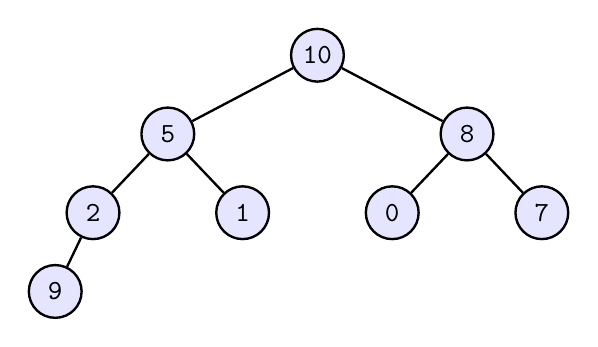
\begin{tikzpicture}

\fill[blue!10] (0.0, 0.0) circle (0.35);
\node [line width=0.03cm,black,minimum size=0.6699999999999999cm,draw,circle] at (0.0,0.0)(10){};\draw (0.0, 0.0) node[color=black] {\texttt{10}};
\fill[blue!10] (-1.9, -1.0) circle (0.35);
\node [line width=0.03cm,black,minimum size=0.6699999999999999cm,draw,circle] at (-1.9,-1.0)(5){};\draw (-1.9, -1.0) node[color=black] {\texttt{5}};
\fill[blue!10] (1.9, -1.0) circle (0.35);
\node [line width=0.03cm,black,minimum size=0.6699999999999999cm,draw,circle] at (1.9,-1.0)(8){};\draw (1.9, -1.0) node[color=black] {\texttt{8}};
\fill[blue!10] (-2.85, -2.0) circle (0.35);
\node [line width=0.03cm,black,minimum size=0.6699999999999999cm,draw,circle] at (-2.85,-2.0)(2){};\draw (-2.85, -2.0) node[color=black] {\texttt{2}};
\fill[blue!10] (-0.95, -2.0) circle (0.35);
\node [line width=0.03cm,black,minimum size=0.6699999999999999cm,draw,circle] at (-0.95,-2.0)(1){};\draw (-0.95, -2.0) node[color=black] {\texttt{1}};
\fill[blue!10] (0.95, -2.0) circle (0.35);
\node [line width=0.03cm,black,minimum size=0.6699999999999999cm,draw,circle] at (0.95,-2.0)(0){};\draw (0.95, -2.0) node[color=black] {\texttt{0}};
\fill[blue!10] (2.85, -2.0) circle (0.35);
\node [line width=0.03cm,black,minimum size=0.6699999999999999cm,draw,circle] at (2.85,-2.0)(7){};\draw (2.85, -2.0) node[color=black] {\texttt{7}};
\fill[blue!10] (-3.33, -3.0) circle (0.35);
\node [line width=0.03cm,black,minimum size=0.6699999999999999cm,draw,circle] at (-3.33,-3.0)(9){};\draw (-3.33, -3.0) node[color=black] {\texttt{9}};\draw[line width=0.03cm,black] (10) to  (5);
\draw[line width=0.03cm,black] (10) to  (8);
\draw[line width=0.03cm,black] (5) to  (2);
\draw[line width=0.03cm,black] (5) to  (1);
\draw[line width=0.03cm,black] (8) to  (0);
\draw[line width=0.03cm,black] (8) to  (7);
\draw[line width=0.03cm,black] (2) to  (9);
\end{tikzpicture}

\end{center}



It's easy to see that in the DFA, the $a$--
and $b$--transitions from the state $\{\}$ goes back to itself.
Therefore the completed DFA is this:


\begin{center}
\begin{tikzpicture}[>=triangle 60,shorten >=0.5pt,node distance=2cm,auto,initial text=, double distance=2pt]
\node[state,initial] (A) at (  0,  0) {$\{q_0\}$};
\node[state] (B) at (  3,  0) {$\{\}$};

\path[->]
(A) edge [bend left=0,pos=0.5,above] node {$a,b$} (B)
(B) edge [loop above] node {$a,b$} ()

;
\end{tikzpicture}
\end{center}
    



\newpage

Solution to Exercise \ref{ex:dfa-as-powerful-as-nfa1}\labeltext{}{sol:dfa-as-powerful-as-nfa1}.

\tinysidebar{\debug{exercises/{dfa-as-powerful-as-nfa1/answer.tex}}}

    Solution not provided.
    

\newpage

Solution to Exercise \ref{ex:dfa-as-powerful-as-nfa2}\labeltext{}{sol:dfa-as-powerful-as-nfa2}.

\tinysidebar{\debug{exercises/{dfa-as-powerful-as-nfa2/answer.tex}}}

    Solution not provided.
    

\newpage

Solution to Exercise \ref{ex:dfa-as-powerful-as-nfa3}\labeltext{}{sol:dfa-as-powerful-as-nfa3}.

\tinysidebar{\debug{exercises/{dfa-as-powerful-as-nfa3/answer.tex}}}

    Solution not provided.
    

\newpage

Solution to Exercise \ref{ex:dfa-as-powerful-as-nfa4}\labeltext{}{sol:dfa-as-powerful-as-nfa4}.

\tinysidebar{\debug{exercises/{dfa-as-powerful-as-nfa4/answer.tex}}}

    Solution not provided.
    

\newpage

Solution to Exercise \ref{ex:closure0}\labeltext{}{sol:closure0}.

\tinysidebar{\debug{exercises/{closure0/answer.tex}}}

    Solution not provided.
    

\newpage

Solution to Exercise \ref{ex:closure1}\labeltext{}{sol:closure1}.

\tinysidebar{\debug{exercises/{closure1/answer.tex}}}

    Solution not provided.
    

\newpage

Solution to Exercise \ref{ex:closure2}\labeltext{}{sol:closure2}.

\tinysidebar{\debug{exercises/{closure2/answer.tex}}}

    Solution not provided.
    

\newpage

Solution to Exercise \ref{ex:closure3}\labeltext{}{sol:closure3}.

\tinysidebar{\debug{exercises/{closure3/answer.tex}}}

    Solution not provided.
    

\newpage

Solution to Exercise \ref{ex:closure4}\labeltext{}{sol:closure4}.

\tinysidebar{\debug{exercises/{closure4/answer.tex}}}

    Solution not provided.
    

\newpage

Solution to Exercise \ref{ex:closure5}\labeltext{}{sol:closure5}.

\tinysidebar{\debug{exercises/{closure5/answer.tex}}}

    Solution not provided.
    

\newpage

Solution to Exercise \ref{ex:closure6}\labeltext{}{sol:closure6}.

\tinysidebar{\debug{exercises/{closure6/answer.tex}}}

    Solution not provided.
    

\newpage

Solution to Exercise \ref{ex:closure7}\labeltext{}{sol:closure7}.

\tinysidebar{\debug{exercises/{closure7/answer.tex}}}

    Solution not provided.
    

\newpage

Solution to Exercise \ref{ex:closure8}\labeltext{}{sol:closure8}.

\tinysidebar{\debug{exercises/{closure8/answer.tex}}}

    Solution not provided.
    

\newpage

Solution to Exercise \ref{ex:closure9}\labeltext{}{sol:closure9}.

\tinysidebar{\debug{exercises/{closure9/answer.tex}}}

    Solution not provided.
    

\newpage

Solution to Exercise \ref{ex:closure10}\labeltext{}{sol:closure10}.

\tinysidebar{\debug{exercises/{closure10/answer.tex}}}

    Solution not provided.
    

\newpage

Solution to Exercise \ref{ex:closure11}\labeltext{}{sol:closure11}.

\tinysidebar{\debug{exercises/{closure11/answer.tex}}}

    Solution not provided.
    

\newpage

Solution to Exercise \ref{ex:closure12}\labeltext{}{sol:closure12}.

\tinysidebar{\debug{exercises/{closure12/answer.tex}}}

    Solution not provided.
    


\newpage%-*-latex-*-
\sectionthree{Linear recursive runtime}
\begin{python0}
from solutions import *; clear()
\end{python0}

So you see that when you measure the runtime of an algorithm
like our Fibonacci function implemented with linear recursion
will give you a runtime function that looks rather similar.
So the next step is to convert the runtime function
to a \textit{non-recursive} closed form.

Before I show you the closed form for the runtime of Fibonacci, let's just get a feel the
such runtime functions by calculating with one.
It turns out that it's pretty bad.

Suppose I need to solve the problem of computing this
function (it's somewhat like my Fibonacci).
Note that $g(n)$ is defined by linear recursion.
\begin{align*}
g(n) = 
\begin{cases}
1                     & \text{ if $n = 0$} \\
3                     & \text{ if $n = 1$} \\
2g(n - 1) + 3g(n - 2) & \text{ if $n \geq 2$}
\end{cases}
\end{align*}
Suppose I choose to write my algorithm like this:
\begin{Verbatim}[frame=single,fontsize=\footnotesize]
def g(n):
    if n == 0: 
        return 1
    elif n == 1:
        return 3
    else:
        return 2 * g(n - 1) + 3 * g(n - 2)
\end{Verbatim}
You know that the runtime function would be like this:
\[
T(n) = 
\begin{cases}
A                     & \text{if $n = 0, 1$} \\
T(n-1) + T(n-2) + B & \text{if $n > 1$}
\end{cases}
\]
for some constants $A$ and $B$.
Later I'll show you now to compute an approximation (in the big-O sense)
for $T(n)$.
For now, suppose we compute $g(5)$ using the above 
program, compute like what a program would, executing one statement
or one operation at a time.
This is what you would see:

\begin{align*}
g(5)
&= 2g(4) + 3g(3) \\
&= 2(2g(3) + 3g(2)) + 3g(3) \\
&= 2(2(2g(2) + 3g(1)) + 3g(2)) + 3g(3) \\
&= 2(2(2(2g(1) + 3g(0)) + 3g(1)) + 3g(2)) + 3g(3) \\
&= 2(2(2(2(3) + 3g(0)) + 3g(1)) + 3g(2)) + 3g(3) \\
&= 2(2(2(6 + 3g(0)) + 3g(1)) + 3g(2)) + 3g(3) \\
&= 2(2(2(6 + 3(1)) + 3g(1)) + 3g(2)) + 3g(3) \\
&= 2(2(2(6 + 3) + 3g(1)) + 3g(2)) + 3g(3) \\
&= 2(2(2(9) + 3g(1)) + 3g(2)) + 3g(3) \\
&= 2(2(18 + 3g(1)) + 3g(2)) + 3g(3) \\
&= 2(2(18 + 3(3)) + 3g(2)) + 3g(3) \\
&= 2(2(18 + 9) + 3g(2)) + 3g(3) \\
&= 2(2(27) + 3g(2)) + 3g(3) \\
&= 2(54 + 3g(2)) + 3g(3) & & \text{will this ever end?!?} \\
&= 2(54 + 3(2g(1) + 3g(0))) + 3g(3) \\
&= 2(54 + 3(2(3) + 3g(0))) + 3g(3) \\
&= 2(54 + 3(6 + 3g(0))) + 3g(3) \\
&= 2(54 + 3(6 + 3(1))) + 3g(3) \\
&= 2(54 + 3(6 + 3)) + 3g(3) \\
&= 2(54 + 3(9)) + 3g(3) \\
&= 2(54 + 27) + 3g(3) \\
&= 2(81) + 3g(3) \\
&= 162 + 3g(3) \\
&= 162 + 3(2g(2) + 3g(1)) & & \text{ ... oh no ... here we go again ...}\\
&= 162 + 3(2(2g(1) + 3g(0)) + 3g(1)) \\
&= 162 + 3(2(2(3) + 3g(0)) + 3g(1)) \\
&= 162 + 3(2(6 + 3g(0)) + 3g(1)) \\
&= 162 + 3(2(6 + 3(1)) + 3g(1)) \\
&= 162 + 3(2(6 + 3) + 3g(1)) \\
&= 162 + 3(2(9) + 3g(1)) \\
&= 162 + 3(18 + 3g(1)) \\
&= 162 + 3(18 + 3(3)) \\
&= 162 + 3(18 + 9) \\
&= 162 + 3(27) \\
&= 162 + 81 \\
&= 243 & & \text{PHEW!!!}
\end{align*}

\begin{ex}
  Show that if \verb!g(n)! is the following
\begin{Verbatim}[frame=single,fontsize=\footnotesize]
def g(n):
    if n == 0: 
        return 1
    elif n == 1:
        return 3
    else:
        return 2 * g(n - 1) + 3 * g(n - 2)
\end{Verbatim}
Then the runtime is $T(n) = O(2^n)$. (This is the not best big-O.)
What is the space complexity?
\end{ex}

\begin{ex}
  Let
\begin{Verbatim}[frame=single,fontsize=\footnotesize]
def h(n):
    if n == 0: 
        return 1
    elif n == 1:
        return 2
    elif n == 2:
        return 42
    else:
        return 7 * h(n - 1) - 3 * h(n - 2) + 4 * h(n - 3)
\end{Verbatim}
What is a big-O of $T(n)$ for \verb!h(n)!?
What is the space complexity?
\end{ex}


So the execution of $g(5)$ using the above algorithm
seems to indicate that $T(5)$ is huge.
You can see even from this simple simulation that the main
problem is that many function calls were actually repeats.
For instance go ahead and count the number of times
$g(2)$ was executed in the above.

It turns out that except for recursion like this:
\begin{Verbatim}[frame=single,fontsize=\footnotesize]
def h(n):
    if n == 0:
        return 42
    else:
        return 7 * h(n - 1) + n
\end{Verbatim}
where in the recursive part only \textit{one} recursive function call was made,
most cases will usually be extremely bad, as in exponential bad.

It turns out that in general if you have a numeric recursive function
like
\[
T(n) = aT(n - 1) + bT(n - 2) + c
\]
where $a$, $b$, and $c$ are constants,
you can always compute a nice formula for $T(n)$.
A \lq\lq nice'' formula for $T(n)$ that does \textit{not} depend on 
$T(i)$ for smaller $i$ but only on $n$, i.e.,
you can compute a closed form formula for $T(n)$.

In fact more generally there are extremely powerful 
tools to compute an \textit{exact} closed form for more complicated
recursion such as 
\[
T(n) = n^2 T(n-1) + (1 + n) T(n - 2) + \frac{2}{3}n^2 - 1 
\]
But I'll stick to the simple case of
\[
T(n) = aT(n - 1) + bT(n - 2) + c
\]
where $a,b,c$ are constants.

Although there are techniques to compute exact closed forms for $T(n)$,
remember that we only need the big-O of $T(n)$.

For the case of a recursive function such as 
\begin{Verbatim}[frame=single,fontsize=\footnotesize]
def g(n):
    if n == 0: 
        return 1
    elif n == 1:
        return 3
    else:
        return 2 * g(n - 1) + 3 * g(n - 2)
\end{Verbatim}
which has a runtime $T(n)$ satisfying
\[
T(n) = T(n - 1) + T(n - 2) + A
\]
where $A$ is a constant, a rough approximation (using the method
in an earlier section) the runtime is
\[
T(n) = O(2^n)
\]
i.e., exponential.
Which means the runtime is bad.
How bad? What exactly is \lq\lq exponential bad"?
You can use the fibonacci function as an example:
\begin{Verbatim}[frame=single,fontsize=\footnotesize]
def fib(n):
    if n == 0: 
        return 1
    elif n == 1:
        return 1
    else:
        return fib(n - 1) + fib(n - 2)
\end{Verbatim}
and print \verb!fib(n)! for \verb!n = 0, 1, 2, ..., 100!.
Remember we did this before in CISS245.
It will grind to a halt before hitting \verb!60!.

In the above, instead of $O(2^n)$, we can be more precise.

First, you ignore the constant $c$ in
\[
T(n) = aT(n - 1) + bT(n - 2) + c \tag{1}
\]
and look at this recursion instead:
\[
T^{(h)}(n) = aT^{(h)}(n - 1) + bT^{(h)}(n - 2) \tag{2}
\]
This is called the \defone{homogeneous part} of $T(n)$.
You need to know that $T^{(h)}(n)$ must have a solution
roughly of the form
\[
T^{(h)}(n) = r^n
\]
where $r$ is a constant.
(Take this on faith for now -- the justification will be
provided in MATH325.)
The immediate goal now is to compute $r$.
You substitute this into (2) to get
\[
r^n = ar^{n-1} + br^{n-2}
\]
You cross out $r^{n - 2}$ to get
\[
r^2 = ar + b
\]
i.e., a quadratic equation.
This then allows you to solve for $r$.

Let's try this technique on our
\[
T(n) = T(n - 1) + T(n - 2) + d
\]
The homogeneous of of this equation is
\[
T^{(h)}(n) = T^{(h)}(n - 1) + T^{(h)}(n - 2)
\]
Let $T^{(h)}(n) = r^n$ and substitute it into
\[
T^{(h)}(n) = T^{(h)}(n - 1) + T^{(h)}(n - 2)
\]
to get
\[
r^n = r^{n - 1} + r^{n - 2}
\]
Cross out $r^{n - 2}$ to get
\[
r^2 = r + 1
\]
which gives us the quadratic
\[
r^2 - r - 1 = 0
\]
Using the quadratic polynomial root formula you get
\[
r = \frac{-(-1) \pm \sqrt{(-1)^2 - 4(1)(-1)} }{2}
\]
which gives us
\[
r = \frac{1 \pm \sqrt{5}}{2}
\]
Let 
\[
r_1 = \frac{1 + \sqrt{5} }{2} 
\]
(... this is the one that is about 1.618)
and 
\[
r_2 = \frac{1 - \sqrt{5} }{2}
\]
Then you know that if the recurrence relation on $T^{(h)}(n)$ is
\[
T^{(h)}(n) = T^{(h)}(n - 1) + T^{(h)}(n - 2)
\]
then $T^{(h)}(n)$ must have the form
\[
T^{(h)}(n) = \alpha \cdot r_1^n + \beta \cdot r_2^n
\]
where $\alpha, \beta$ are constants.

This is the closed form for $T^{(h)}(n)$.
But what about $T(n)$? Remember that
\[
T(n) = T^{(h)}(n) + d
\]
The next thing you need to know is that
if $r_1$ and $r_2$ are both $1$, then
\[
\]

Now, $|r_2| = 0.618...$ whereas $r_1 = 1.618...$.
Therefore
\[
T^{(h)}(n) = \alpha \cdot r_1^n + \beta \cdot r_2^n = O(r_1^n)
\]
which means that the algorithm has exponential runtime
but the base of the exponential runtime is $1.618...$ instead of $2$.
Note that $2^n$ climbs much faster than $1.618^n$.
That's because
\[
\frac{2^n}{1.618^n} = 1.236...^n
\]
and $1.236...^n$ grows toward infinity as $n$ grows unboundedly
since $1.236 > 1$.

Note that at the stage where you solve for $r$ in 
the quadratic equation in $r$:
\[
r^2 = ar + b \tag{*}
\]
you will have \textit{three} cases: $(*)$ has
\begin{align*}
\text{Case 1:} & \ \text{two distinct real roots} \\
\text{Case 2:} & \ \text{two distinct complex (and nonreal) roots} \\
\text{Case 3:} & \ \text{two roots with the same real value}
\end{align*}
The Fibonacci case of 
\[
r^2 = r + 1
\]
gives us two distinct real roots.

For case (a) and (b) above, the $T(n)$ is just
\[
T(n) = \alpha r_1^n + \beta r_2^n
\]
(Unfortunately for case (b) you would have to use complex
numbers.)
For the third case where there is one value $r_1$ for both roots,
the closed form becomes
\[
T(n) = \alpha r_1^n + \beta nr_1^n
\]
so in this case
\[
T(n) = O(nr_1^n)
\]
Of course as for the specific big-O class, you have to 
compute the exact root values.

[EXERCISES]

%\newpage
%\subsection*{Solutions}
%
\newpage
\section*{Solutions}
Solution to Exercise \ref{ex:dfa0}\labeltext{}{sol:dfa0}.

\tinysidebar{\debug{exercises/{dfa0/answer.tex}}}

    Solution not provided.
    

\newpage

Solution to Exercise \ref{ex:dfa1}\labeltext{}{sol:dfa1}.

\tinysidebar{\debug{exercises/{dfa1/answer.tex}}}
  The ID computation is
  \begin{align*}
    (q_0, aba)
    &\vdash (\delta(q_0, a), ba) = (q_0, ba) \\ 
    &\vdash (\delta(q_0, b), a) = (q_1, a) \\
    &\vdash (\delta(q_1, a), \ep) = (q_0, \ep)
  \end{align*}
  $q_0$ is not an accept state. Therefore $aba$ is not accepted.


\newpage

Solution to Exercise \ref{ex:dfa4}\labeltext{}{sol:dfa4}.

\tinysidebar{\debug{exercises/{dfa4/answer.tex}}}

    Solution not provided.
    

\newpage

Solution to Exercise \ref{ex:dfa5}\labeltext{}{sol:dfa5}.

\tinysidebar{\debug{exercises/{dfa5/answer.tex}}}

    Solution not provided.
    

\newpage

Solution to Exercise \ref{ex:implementing-a-single-dfa0}\labeltext{}{sol:implementing-a-single-dfa0}.

\tinysidebar{\debug{exercises/{implementing-a-single-dfa0/answer.tex}}}

    Solution not provided.
    

\newpage

Solution to Exercise \ref{ex:nfastatediag0}\labeltext{}{sol:nfastatediag0}.

\tinysidebar{\debug{exercises/{nfastatediag0/answer.tex}}}

    Solution not provided.
    

\newpage

Solution to Exercise \ref{ex:nfastatediag1}\labeltext{}{sol:nfastatediag1}.

\tinysidebar{\debug{exercises/{nfastatediag1/answer.tex}}}

    Solution not provided.
    

\newpage

Solution to Exercise \ref{ex:nfastatediag2}\labeltext{}{sol:nfastatediag2}.

\tinysidebar{\debug{exercises/{nfastatediag2/answer.tex}}}

    Solution not provided.
    

\newpage

Solution to Exercise \ref{ex:nfastatediag3}\labeltext{}{sol:nfastatediag3}.

\tinysidebar{\debug{exercises/{nfastatediag3/answer.tex}}}

    Solution not provided.
    

\newpage

Solution to Exercise \ref{ex:nfastatediag4}\labeltext{}{sol:nfastatediag4}.

\tinysidebar{\debug{exercises/{nfastatediag4/answer.tex}}}

    Solution not provided.
    

\newpage

Solution to Exercise \ref{ex:nfastatediag5}\labeltext{}{sol:nfastatediag5}.

\tinysidebar{\debug{exercises/{nfastatediag5/answer.tex}}}

    Solution not provided.
    

\newpage

Solution to Exercise \ref{ex:nfastatediag6}\labeltext{}{sol:nfastatediag6}.

\tinysidebar{\debug{exercises/{nfastatediag6/answer.tex}}}

    Solution not provided.
    

\newpage

Solution to Exercise \ref{ex:nfastatediag7}\labeltext{}{sol:nfastatediag7}.

\tinysidebar{\debug{exercises/{nfastatediag7/answer.tex}}}

    Solution not provided.
    

\newpage

Solution to Exercise \ref{ex:nfastatediag8}\labeltext{}{sol:nfastatediag8}.

\tinysidebar{\debug{exercises/{nfastatediag8/answer.tex}}}

    Solution not provided.
    

\newpage

Solution to Exercise \ref{ex:nfastatediag9}\labeltext{}{sol:nfastatediag9}.

\tinysidebar{\debug{exercises/{nfastatediag9/answer.tex}}}

    Solution not provided.
    

\newpage

Solution to Exercise \ref{ex:nfastatediag10}\labeltext{}{sol:nfastatediag10}.

\tinysidebar{\debug{exercises/{nfastatediag10/answer.tex}}}

    Solution not provided.
    

\newpage

Solution to Exercise \ref{ex:nfastatediag11}\labeltext{}{sol:nfastatediag11}.

\tinysidebar{\debug{exercises/{nfastatediag11/answer.tex}}}

    Solution not provided.
    

\newpage

Solution to Exercise \ref{ex:nfastatediag12}\labeltext{}{sol:nfastatediag12}.

\tinysidebar{\debug{exercises/{nfastatediag12/answer.tex}}}

    Solution not provided.
    

\newpage

Solution to Exercise \ref{ex:nfastatediag13}\labeltext{}{sol:nfastatediag13}.

\tinysidebar{\debug{exercises/{nfastatediag13/answer.tex}}}

    Solution not provided.
    

\newpage

Solution to Exercise \ref{ex:nfa0}\labeltext{}{sol:nfa0}.

\tinysidebar{\debug{exercises/{nfa0/answer.tex}}}
The formal definition of this NFA is $(\Sigma, Q, q_0, \delta, F)$ where
\begin{tightlist}
\li $\Sigma = \{a,b\}$
\li $Q = \{q_0\}$
\li $\delta$ is the function
\[
\delta : Q \times \Sigma_\epsilon \rightarrow P(Q)
\]
given by
\begin{align*}
  \delta(q_0, \epsilon) &= \{\} \\
  \delta(q_0, a) &= \{\} \\
  \delta(q_0, b) &= \{\} 
\end{align*}
\end{tightlist}


\newpage

Solution to Exercise \ref{ex:nfa1}\labeltext{}{sol:nfa1}.

\tinysidebar{\debug{exercises/{nfa1/answer.tex}}}

    Solution not provided.
    

\newpage

Solution to Exercise \ref{ex:nfa2}\labeltext{}{sol:nfa2}.

\tinysidebar{\debug{exercises/{nfa2/answer.tex}}}

    Solution not provided.
    

\newpage

Solution to Exercise \ref{ex:nfa3}\labeltext{}{sol:nfa3}.

\tinysidebar{\debug{exercises/{nfa3/answer.tex}}}

    Solution not provided.
    

\newpage

Solution to Exercise \ref{ex:nfa4}\labeltext{}{sol:nfa4}.

\tinysidebar{\debug{exercises/{nfa4/answer.tex}}}

    Solution not provided.
    

\newpage

Solution to Exercise \ref{ex:nfa5}\labeltext{}{sol:nfa5}.

\tinysidebar{\debug{exercises/{nfa5/answer.tex}}}

    Solution not provided.
    

\newpage

Solution to Exercise \ref{ex:dfa-as-powerful-as-nfa0}\labeltext{}{sol:dfa-as-powerful-as-nfa0}.

\tinysidebar{\debug{exercises/{dfa-as-powerful-as-nfa0/answer.tex}}}
Here's the solution.
Let $\delta$ denote the transition function of $N$.
Note that 
\begin{align*}
  \delta(q_0, \epsilon) = \{\} \\
  \delta(q_0, a) = \{\} \\
  \delta(q_0, b) = \{\} 
\end{align*}
First of all the states are labeled as all the subsets of $\{q_0\}$.


\begin{center}
\begin{tikzpicture}[>=triangle 60,shorten >=0.5pt,node distance=2cm,auto,initial text=, double distance=2pt]
\node[state] (A) at (  0,  0) {$\{q_0\}$};
\node[state] (B) at (  3,  0) {$\{\}$};

\path[->]

;
\end{tikzpicture}
\end{center}
    


The start state is the $\epsilon$-closure of $\{q_0\}$.
However in $N$, there are no $\epsilon$--transitions out of 
$q_0$.
So the $\epsilon$-closure of $\{q_0\}$ is in fact $\{q_0\}$, i.e.
$\overline{\{q_0\}} = \{q_0\}$
The $\DFA$ is now this:


\begin{longtable}{|r||r|r|r|r|r|}
\hline 
         & $w_1$ & $w_2$ & $w_3$ & $w_4$ & $\ldots$ \\ \hline \hline 
$M_1$    &       &       &       &       &          \\ \hline 
$M_2$    &       &       &       &       &          \\ \hline 
$M_3$    &       &       &       &       &          \\ \hline 
$M_4$    &       &       &       &       &          \\ \hline 
$\ldots$ &       &       &       &       &          \\ \hline 
\end{longtable}
        


Now I will compute the $a$--transition of the state $\{q_0\}$.
Let $\delta^\DFA$ denote the transition function of the $\DFA$
that we're building.
Then
\begin{align*}
\delta( \{q_0, a\} ) 
&= \overline{ \bigcup_{q \in \{q_0\}} \delta(q, a)} \\
&= \overline{ \delta(q_0, a) } \\
&= \overline{ \emptyset } \\
&= \emptyset
\end{align*}
The (incomplete) $\DFA$ now looks like this:


\begin{longtable}{|r||r|r|r|r|r|}
\hline 
         & $w_1$ & $w_2$ & $w_3$ & $w_4$ & $\ldots$ \\ \hline \hline 
$M_1$    & 0     & 0     & 1     & 0     & ...      \\ \hline 
$M_2$    & 1     & 0     & 1     & 1     & ...      \\ \hline 
$M_3$    & 0     & 1     & 1     & 1     & ...      \\ \hline 
$M_4$    & 1     & 0     & 1     & 1     & ...      \\ \hline 
$\ldots$ &       &       &       &       &          \\ \hline 
\end{longtable}
        


Using the same reasoning we have

\begin{center}
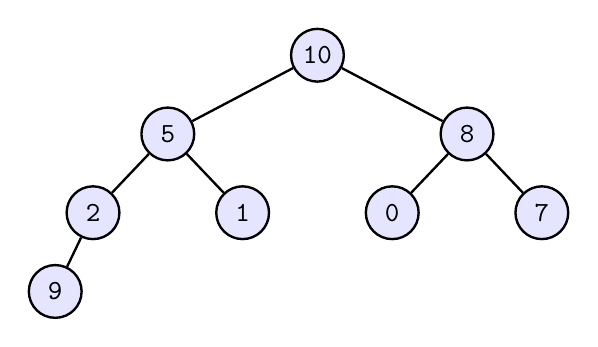
\begin{tikzpicture}

\fill[blue!10] (0.0, 0.0) circle (0.35);
\node [line width=0.03cm,black,minimum size=0.6699999999999999cm,draw,circle] at (0.0,0.0)(10){};\draw (0.0, 0.0) node[color=black] {\texttt{10}};
\fill[blue!10] (-1.9, -1.0) circle (0.35);
\node [line width=0.03cm,black,minimum size=0.6699999999999999cm,draw,circle] at (-1.9,-1.0)(5){};\draw (-1.9, -1.0) node[color=black] {\texttt{5}};
\fill[blue!10] (1.9, -1.0) circle (0.35);
\node [line width=0.03cm,black,minimum size=0.6699999999999999cm,draw,circle] at (1.9,-1.0)(8){};\draw (1.9, -1.0) node[color=black] {\texttt{8}};
\fill[blue!10] (-2.85, -2.0) circle (0.35);
\node [line width=0.03cm,black,minimum size=0.6699999999999999cm,draw,circle] at (-2.85,-2.0)(2){};\draw (-2.85, -2.0) node[color=black] {\texttt{2}};
\fill[blue!10] (-0.95, -2.0) circle (0.35);
\node [line width=0.03cm,black,minimum size=0.6699999999999999cm,draw,circle] at (-0.95,-2.0)(1){};\draw (-0.95, -2.0) node[color=black] {\texttt{1}};
\fill[blue!10] (0.95, -2.0) circle (0.35);
\node [line width=0.03cm,black,minimum size=0.6699999999999999cm,draw,circle] at (0.95,-2.0)(0){};\draw (0.95, -2.0) node[color=black] {\texttt{0}};
\fill[blue!10] (2.85, -2.0) circle (0.35);
\node [line width=0.03cm,black,minimum size=0.6699999999999999cm,draw,circle] at (2.85,-2.0)(7){};\draw (2.85, -2.0) node[color=black] {\texttt{7}};
\fill[blue!10] (-3.33, -3.0) circle (0.35);
\node [line width=0.03cm,black,minimum size=0.6699999999999999cm,draw,circle] at (-3.33,-3.0)(9){};\draw (-3.33, -3.0) node[color=black] {\texttt{9}};\draw[line width=0.03cm,black] (10) to  (5);
\draw[line width=0.03cm,black] (10) to  (8);
\draw[line width=0.03cm,black] (5) to  (2);
\draw[line width=0.03cm,black] (5) to  (1);
\draw[line width=0.03cm,black] (8) to  (0);
\draw[line width=0.03cm,black] (8) to  (7);
\draw[line width=0.03cm,black] (2) to  (9);
\end{tikzpicture}

\end{center}



It's easy to see that in the DFA, the $a$--
and $b$--transitions from the state $\{\}$ goes back to itself.
Therefore the completed DFA is this:


\begin{center}
\begin{tikzpicture}[>=triangle 60,shorten >=0.5pt,node distance=2cm,auto,initial text=, double distance=2pt]
\node[state,initial] (A) at (  0,  0) {$\{q_0\}$};
\node[state] (B) at (  3,  0) {$\{\}$};

\path[->]
(A) edge [bend left=0,pos=0.5,above] node {$a,b$} (B)
(B) edge [loop above] node {$a,b$} ()

;
\end{tikzpicture}
\end{center}
    



\newpage

Solution to Exercise \ref{ex:dfa-as-powerful-as-nfa1}\labeltext{}{sol:dfa-as-powerful-as-nfa1}.

\tinysidebar{\debug{exercises/{dfa-as-powerful-as-nfa1/answer.tex}}}

    Solution not provided.
    

\newpage

Solution to Exercise \ref{ex:dfa-as-powerful-as-nfa2}\labeltext{}{sol:dfa-as-powerful-as-nfa2}.

\tinysidebar{\debug{exercises/{dfa-as-powerful-as-nfa2/answer.tex}}}

    Solution not provided.
    

\newpage

Solution to Exercise \ref{ex:dfa-as-powerful-as-nfa3}\labeltext{}{sol:dfa-as-powerful-as-nfa3}.

\tinysidebar{\debug{exercises/{dfa-as-powerful-as-nfa3/answer.tex}}}

    Solution not provided.
    

\newpage

Solution to Exercise \ref{ex:dfa-as-powerful-as-nfa4}\labeltext{}{sol:dfa-as-powerful-as-nfa4}.

\tinysidebar{\debug{exercises/{dfa-as-powerful-as-nfa4/answer.tex}}}

    Solution not provided.
    

\newpage

Solution to Exercise \ref{ex:closure0}\labeltext{}{sol:closure0}.

\tinysidebar{\debug{exercises/{closure0/answer.tex}}}

    Solution not provided.
    

\newpage

Solution to Exercise \ref{ex:closure1}\labeltext{}{sol:closure1}.

\tinysidebar{\debug{exercises/{closure1/answer.tex}}}

    Solution not provided.
    

\newpage

Solution to Exercise \ref{ex:closure2}\labeltext{}{sol:closure2}.

\tinysidebar{\debug{exercises/{closure2/answer.tex}}}

    Solution not provided.
    

\newpage

Solution to Exercise \ref{ex:closure3}\labeltext{}{sol:closure3}.

\tinysidebar{\debug{exercises/{closure3/answer.tex}}}

    Solution not provided.
    

\newpage

Solution to Exercise \ref{ex:closure4}\labeltext{}{sol:closure4}.

\tinysidebar{\debug{exercises/{closure4/answer.tex}}}

    Solution not provided.
    

\newpage

Solution to Exercise \ref{ex:closure5}\labeltext{}{sol:closure5}.

\tinysidebar{\debug{exercises/{closure5/answer.tex}}}

    Solution not provided.
    

\newpage

Solution to Exercise \ref{ex:closure6}\labeltext{}{sol:closure6}.

\tinysidebar{\debug{exercises/{closure6/answer.tex}}}

    Solution not provided.
    

\newpage

Solution to Exercise \ref{ex:closure7}\labeltext{}{sol:closure7}.

\tinysidebar{\debug{exercises/{closure7/answer.tex}}}

    Solution not provided.
    

\newpage

Solution to Exercise \ref{ex:closure8}\labeltext{}{sol:closure8}.

\tinysidebar{\debug{exercises/{closure8/answer.tex}}}

    Solution not provided.
    

\newpage

Solution to Exercise \ref{ex:closure9}\labeltext{}{sol:closure9}.

\tinysidebar{\debug{exercises/{closure9/answer.tex}}}

    Solution not provided.
    

\newpage

Solution to Exercise \ref{ex:closure10}\labeltext{}{sol:closure10}.

\tinysidebar{\debug{exercises/{closure10/answer.tex}}}

    Solution not provided.
    

\newpage

Solution to Exercise \ref{ex:closure11}\labeltext{}{sol:closure11}.

\tinysidebar{\debug{exercises/{closure11/answer.tex}}}

    Solution not provided.
    

\newpage

Solution to Exercise \ref{ex:closure12}\labeltext{}{sol:closure12}.

\tinysidebar{\debug{exercises/{closure12/answer.tex}}}

    Solution not provided.
    


\newpage%-*-latex-*-
\sectionthree{Speeding up linear recursion}
\begin{python0}
from solutions import *; clear()
\end{python0}

Recall that if you have a runtime that is like this:
\[
T(n) 
= 
\begin{cases}
A                   & \text{if $n = 0, 1$} \\
T(n-1) + T(n-2) + B & \text{otherwise}
\end{cases}
\]
which is the case for the Fibonacci function:
\begin{Verbatim}[frame=single,fontsize=\footnotesize]
def fib(n):
    if n < 2:
        return 1
    else:
        return fib(n - 1) + fib(n - 2)
\end{Verbatim}
then the runtime is exponential:
\[
T(n) = O(2^n)
\]

When you look at the computation of the degree 2 linear recurrence
computation-by-hand in a previous section, 
you see that the problem is the repeated computations of 
\verb!fib(i)!
(\verb!i = n - 2, ...!) when you compute \verb!fib(n)!.

One way to prevent re-computation is to ... save your work!!!
So let's say we have an array \verb!table! of size 1000
to store \verb!fib(0)!, \verb!fib(1)!, ..., \verb!fib(999)!.
Initially, the table is empty.
To indicate that \verb!table[i]! is \lq\lq empty'',
I'll set it to $-1$ since the Fibonacci numbers are positive.

Then, whenever I compute \verb!fib(n)!, I first check if it's already in the 
\verb!table!.
If it is, I'll use the number.
If it's not, I'll compute \verb!fib(n)!, save it in the table,
then return it.
Now the function looks like this:
 
\begin{Verbatim}[frame=single,fontsize=\footnotesize]
for i = 0, ..., 999:
    table[i] = -1

def fib(n):
    if n < 2:
        return 1
    else:
        if table[n] is -1:
            table[n] = fib(n - 1) + fib(n - 2)
        return table[n]
\end{Verbatim}

This is not new.
you have already seen this technique in CISS245.
The concept of storing computations in a table to avoid
re-computation is extremely important and appears
in a huge number of algorithms (not just fibonacci computations).

\newpage
\begin{ex}
  Assuming your \verb!table! is large enough to store
  all computation of
  \verb!fib(0)!,
  \verb!fib(1)!,
  \verb!fib(2)!,
  \verb!fib(3)!,
  ...,
  \verb!fib(n)!,
  compute the runtime 
  of the above implementation.
\qed
\end{ex}

Of course it's possible that you want $f(10000000)$.
You can either increase your the size of your \verb!table!
or simply use the \verb!table! only when \verb!n! is less than 1000.

\newpage
\begin{ex}
Modify the above problem to use the \verb!table! only when 
\verb!n! is less than 1000.
\end{ex}


\begin{comment}
\newpage
\begin{ex}
Note that we use \verb!table[5]! to store $f(5)$, i.e.,
\verb!table[0, ..., 999]! corresponds to 
$f(0), ..., f(999)$.
What if you want to store 
$f(10)$, ..., $f(1009)$ in \verb!table[0,...,999]! instead?
\end{ex}
\end{comment}

\newpage
Notice that the above method requires storage to save computations
in order to prevent re-computation.
There's another way to compute the $n$--th Fibonacci without too much 
storage space.
Here's the idea:
Instead of compute \lq\lq top-to-bottom''
(i.e., going from $n$ to $1$ and $0$)
you start at $0$ and $1$ and compute up to $n$.
Here's an execution of $f(6)$.
First of all, the Fibonacci numbers up the the $6$--th is this:
\begin{Verbatim}[frame=single, fontsize=\footnotesize]
1, 1, 2, 3, 5, 8, 13
\end{Verbatim}
You need only 3 variables.
I'll call them $a, b, c$.
First you set $a,b,c$ to these values:
\begin{Verbatim}[frame=single, fontsize=\footnotesize]
1, 1, 2, 3, 5, 8, 13
a  b  c
\end{Verbatim}
In other words $c = a + b$ after initializing $a$ and $b$ to 1.
Next you want to perform some computation to get this:
\begin{Verbatim}[frame=single, fontsize=\footnotesize]
1, 1, 2, 3, 5, 8, 13
   a  b  c
\end{Verbatim}
Next you want to perform some computation to get this:
\begin{Verbatim}[frame=single, fontsize=\footnotesize]
1, 1, 2, 3, 5, 8, 13
      a  b  c
\end{Verbatim}
and then this:
\begin{Verbatim}[frame=single, fontsize=\footnotesize]
1, 1, 2, 3, 5, 8, 13
         a  b  c
\end{Verbatim}
and finally this:
\begin{Verbatim}[frame=single, fontsize=\footnotesize]
1, 1, 2, 3, 5, 8, 13
            a  b  c
\end{Verbatim}
Basically \verb!a! plays the role of \verb!f(i - 2)!, 
\verb!b! plays the role of \verb!f(i - 1)!, 
and \verb!c! plays the role of \verb!f(i)!.
You run your \verb!i! from \verb!i = 2! to \verb!i = n!.

I'm going to call this the \defone{bottom-up} technique. 
You can use a for-loop or recursion to implement a
bottom-up algorithm.


\newpage
\begin{ex}
Implement this new Fibonacci function (a) using a for-loop and 
(b) using recursion.
Test them.
Compute the runtime.
\qed
\end{ex}


\newpage
\begin{ex}
The following is a linear recursion:
\begin{Verbatim}[frame=single, fontsize=\footnotesize]
def f(n):
    if n == 0:
        return 1
    elif n == 1:
        return 2
    else:
        return f(n - 1) + 3 * f(n - 2) + 1
\end{Verbatim}
Run this and compute \verb!f(0)!, \verb!f(1)!, ..., \verb!f(50)!.
Notice that it slows down tremendously.
Compute the runtime of this implementation.
Re-implement this using the bottom-to-top technique
(first using a for-loop and next using recursion.)
\qed
\end{ex}


\newpage
\begin{ex}
The following is a linear recursion:
\begin{Verbatim}[frame=single, fontsize=\footnotesize]
def f(n):
    if n == 0:
        return 0
    elif n == 1:
        return 1
    elif n == 2:
        return 2
    else:
        return f(n - 1) + 2*f(n - 2) + 3*f(n - 3) 
\end{Verbatim}
Run this and compute $f(0)$, $f(1)$, ..., $f(50)$.
Notice that it slows down tremendously.
Compute the runtime of this implementation.
Re-implement this using the bottom-to-top technique
(first using a for-loop and next using recursion.)
\qed
\end{ex}

%\newpage
%\subsection*{Solutions}
%
\newpage
\section*{Solutions}
Solution to Exercise \ref{ex:dfa0}\labeltext{}{sol:dfa0}.

\tinysidebar{\debug{exercises/{dfa0/answer.tex}}}

    Solution not provided.
    

\newpage

Solution to Exercise \ref{ex:dfa1}\labeltext{}{sol:dfa1}.

\tinysidebar{\debug{exercises/{dfa1/answer.tex}}}
  The ID computation is
  \begin{align*}
    (q_0, aba)
    &\vdash (\delta(q_0, a), ba) = (q_0, ba) \\ 
    &\vdash (\delta(q_0, b), a) = (q_1, a) \\
    &\vdash (\delta(q_1, a), \ep) = (q_0, \ep)
  \end{align*}
  $q_0$ is not an accept state. Therefore $aba$ is not accepted.


\newpage

Solution to Exercise \ref{ex:dfa4}\labeltext{}{sol:dfa4}.

\tinysidebar{\debug{exercises/{dfa4/answer.tex}}}

    Solution not provided.
    

\newpage

Solution to Exercise \ref{ex:dfa5}\labeltext{}{sol:dfa5}.

\tinysidebar{\debug{exercises/{dfa5/answer.tex}}}

    Solution not provided.
    

\newpage

Solution to Exercise \ref{ex:implementing-a-single-dfa0}\labeltext{}{sol:implementing-a-single-dfa0}.

\tinysidebar{\debug{exercises/{implementing-a-single-dfa0/answer.tex}}}

    Solution not provided.
    

\newpage

Solution to Exercise \ref{ex:nfastatediag0}\labeltext{}{sol:nfastatediag0}.

\tinysidebar{\debug{exercises/{nfastatediag0/answer.tex}}}

    Solution not provided.
    

\newpage

Solution to Exercise \ref{ex:nfastatediag1}\labeltext{}{sol:nfastatediag1}.

\tinysidebar{\debug{exercises/{nfastatediag1/answer.tex}}}

    Solution not provided.
    

\newpage

Solution to Exercise \ref{ex:nfastatediag2}\labeltext{}{sol:nfastatediag2}.

\tinysidebar{\debug{exercises/{nfastatediag2/answer.tex}}}

    Solution not provided.
    

\newpage

Solution to Exercise \ref{ex:nfastatediag3}\labeltext{}{sol:nfastatediag3}.

\tinysidebar{\debug{exercises/{nfastatediag3/answer.tex}}}

    Solution not provided.
    

\newpage

Solution to Exercise \ref{ex:nfastatediag4}\labeltext{}{sol:nfastatediag4}.

\tinysidebar{\debug{exercises/{nfastatediag4/answer.tex}}}

    Solution not provided.
    

\newpage

Solution to Exercise \ref{ex:nfastatediag5}\labeltext{}{sol:nfastatediag5}.

\tinysidebar{\debug{exercises/{nfastatediag5/answer.tex}}}

    Solution not provided.
    

\newpage

Solution to Exercise \ref{ex:nfastatediag6}\labeltext{}{sol:nfastatediag6}.

\tinysidebar{\debug{exercises/{nfastatediag6/answer.tex}}}

    Solution not provided.
    

\newpage

Solution to Exercise \ref{ex:nfastatediag7}\labeltext{}{sol:nfastatediag7}.

\tinysidebar{\debug{exercises/{nfastatediag7/answer.tex}}}

    Solution not provided.
    

\newpage

Solution to Exercise \ref{ex:nfastatediag8}\labeltext{}{sol:nfastatediag8}.

\tinysidebar{\debug{exercises/{nfastatediag8/answer.tex}}}

    Solution not provided.
    

\newpage

Solution to Exercise \ref{ex:nfastatediag9}\labeltext{}{sol:nfastatediag9}.

\tinysidebar{\debug{exercises/{nfastatediag9/answer.tex}}}

    Solution not provided.
    

\newpage

Solution to Exercise \ref{ex:nfastatediag10}\labeltext{}{sol:nfastatediag10}.

\tinysidebar{\debug{exercises/{nfastatediag10/answer.tex}}}

    Solution not provided.
    

\newpage

Solution to Exercise \ref{ex:nfastatediag11}\labeltext{}{sol:nfastatediag11}.

\tinysidebar{\debug{exercises/{nfastatediag11/answer.tex}}}

    Solution not provided.
    

\newpage

Solution to Exercise \ref{ex:nfastatediag12}\labeltext{}{sol:nfastatediag12}.

\tinysidebar{\debug{exercises/{nfastatediag12/answer.tex}}}

    Solution not provided.
    

\newpage

Solution to Exercise \ref{ex:nfastatediag13}\labeltext{}{sol:nfastatediag13}.

\tinysidebar{\debug{exercises/{nfastatediag13/answer.tex}}}

    Solution not provided.
    

\newpage

Solution to Exercise \ref{ex:nfa0}\labeltext{}{sol:nfa0}.

\tinysidebar{\debug{exercises/{nfa0/answer.tex}}}
The formal definition of this NFA is $(\Sigma, Q, q_0, \delta, F)$ where
\begin{tightlist}
\li $\Sigma = \{a,b\}$
\li $Q = \{q_0\}$
\li $\delta$ is the function
\[
\delta : Q \times \Sigma_\epsilon \rightarrow P(Q)
\]
given by
\begin{align*}
  \delta(q_0, \epsilon) &= \{\} \\
  \delta(q_0, a) &= \{\} \\
  \delta(q_0, b) &= \{\} 
\end{align*}
\end{tightlist}


\newpage

Solution to Exercise \ref{ex:nfa1}\labeltext{}{sol:nfa1}.

\tinysidebar{\debug{exercises/{nfa1/answer.tex}}}

    Solution not provided.
    

\newpage

Solution to Exercise \ref{ex:nfa2}\labeltext{}{sol:nfa2}.

\tinysidebar{\debug{exercises/{nfa2/answer.tex}}}

    Solution not provided.
    

\newpage

Solution to Exercise \ref{ex:nfa3}\labeltext{}{sol:nfa3}.

\tinysidebar{\debug{exercises/{nfa3/answer.tex}}}

    Solution not provided.
    

\newpage

Solution to Exercise \ref{ex:nfa4}\labeltext{}{sol:nfa4}.

\tinysidebar{\debug{exercises/{nfa4/answer.tex}}}

    Solution not provided.
    

\newpage

Solution to Exercise \ref{ex:nfa5}\labeltext{}{sol:nfa5}.

\tinysidebar{\debug{exercises/{nfa5/answer.tex}}}

    Solution not provided.
    

\newpage

Solution to Exercise \ref{ex:dfa-as-powerful-as-nfa0}\labeltext{}{sol:dfa-as-powerful-as-nfa0}.

\tinysidebar{\debug{exercises/{dfa-as-powerful-as-nfa0/answer.tex}}}
Here's the solution.
Let $\delta$ denote the transition function of $N$.
Note that 
\begin{align*}
  \delta(q_0, \epsilon) = \{\} \\
  \delta(q_0, a) = \{\} \\
  \delta(q_0, b) = \{\} 
\end{align*}
First of all the states are labeled as all the subsets of $\{q_0\}$.


\begin{center}
\begin{tikzpicture}[>=triangle 60,shorten >=0.5pt,node distance=2cm,auto,initial text=, double distance=2pt]
\node[state] (A) at (  0,  0) {$\{q_0\}$};
\node[state] (B) at (  3,  0) {$\{\}$};

\path[->]

;
\end{tikzpicture}
\end{center}
    


The start state is the $\epsilon$-closure of $\{q_0\}$.
However in $N$, there are no $\epsilon$--transitions out of 
$q_0$.
So the $\epsilon$-closure of $\{q_0\}$ is in fact $\{q_0\}$, i.e.
$\overline{\{q_0\}} = \{q_0\}$
The $\DFA$ is now this:


\begin{longtable}{|r||r|r|r|r|r|}
\hline 
         & $w_1$ & $w_2$ & $w_3$ & $w_4$ & $\ldots$ \\ \hline \hline 
$M_1$    &       &       &       &       &          \\ \hline 
$M_2$    &       &       &       &       &          \\ \hline 
$M_3$    &       &       &       &       &          \\ \hline 
$M_4$    &       &       &       &       &          \\ \hline 
$\ldots$ &       &       &       &       &          \\ \hline 
\end{longtable}
        


Now I will compute the $a$--transition of the state $\{q_0\}$.
Let $\delta^\DFA$ denote the transition function of the $\DFA$
that we're building.
Then
\begin{align*}
\delta( \{q_0, a\} ) 
&= \overline{ \bigcup_{q \in \{q_0\}} \delta(q, a)} \\
&= \overline{ \delta(q_0, a) } \\
&= \overline{ \emptyset } \\
&= \emptyset
\end{align*}
The (incomplete) $\DFA$ now looks like this:


\begin{longtable}{|r||r|r|r|r|r|}
\hline 
         & $w_1$ & $w_2$ & $w_3$ & $w_4$ & $\ldots$ \\ \hline \hline 
$M_1$    & 0     & 0     & 1     & 0     & ...      \\ \hline 
$M_2$    & 1     & 0     & 1     & 1     & ...      \\ \hline 
$M_3$    & 0     & 1     & 1     & 1     & ...      \\ \hline 
$M_4$    & 1     & 0     & 1     & 1     & ...      \\ \hline 
$\ldots$ &       &       &       &       &          \\ \hline 
\end{longtable}
        


Using the same reasoning we have

\begin{center}
\begin{tikzpicture}

\fill[blue!10] (0.0, 0.0) circle (0.35);
\node [line width=0.03cm,black,minimum size=0.6699999999999999cm,draw,circle] at (0.0,0.0)(10){};\draw (0.0, 0.0) node[color=black] {\texttt{10}};
\fill[blue!10] (-1.9, -1.0) circle (0.35);
\node [line width=0.03cm,black,minimum size=0.6699999999999999cm,draw,circle] at (-1.9,-1.0)(5){};\draw (-1.9, -1.0) node[color=black] {\texttt{5}};
\fill[blue!10] (1.9, -1.0) circle (0.35);
\node [line width=0.03cm,black,minimum size=0.6699999999999999cm,draw,circle] at (1.9,-1.0)(8){};\draw (1.9, -1.0) node[color=black] {\texttt{8}};
\fill[blue!10] (-2.85, -2.0) circle (0.35);
\node [line width=0.03cm,black,minimum size=0.6699999999999999cm,draw,circle] at (-2.85,-2.0)(2){};\draw (-2.85, -2.0) node[color=black] {\texttt{2}};
\fill[blue!10] (-0.95, -2.0) circle (0.35);
\node [line width=0.03cm,black,minimum size=0.6699999999999999cm,draw,circle] at (-0.95,-2.0)(1){};\draw (-0.95, -2.0) node[color=black] {\texttt{1}};
\fill[blue!10] (0.95, -2.0) circle (0.35);
\node [line width=0.03cm,black,minimum size=0.6699999999999999cm,draw,circle] at (0.95,-2.0)(0){};\draw (0.95, -2.0) node[color=black] {\texttt{0}};
\fill[blue!10] (2.85, -2.0) circle (0.35);
\node [line width=0.03cm,black,minimum size=0.6699999999999999cm,draw,circle] at (2.85,-2.0)(7){};\draw (2.85, -2.0) node[color=black] {\texttt{7}};
\fill[blue!10] (-3.33, -3.0) circle (0.35);
\node [line width=0.03cm,black,minimum size=0.6699999999999999cm,draw,circle] at (-3.33,-3.0)(9){};\draw (-3.33, -3.0) node[color=black] {\texttt{9}};\draw[line width=0.03cm,black] (10) to  (5);
\draw[line width=0.03cm,black] (10) to  (8);
\draw[line width=0.03cm,black] (5) to  (2);
\draw[line width=0.03cm,black] (5) to  (1);
\draw[line width=0.03cm,black] (8) to  (0);
\draw[line width=0.03cm,black] (8) to  (7);
\draw[line width=0.03cm,black] (2) to  (9);
\end{tikzpicture}

\end{center}



It's easy to see that in the DFA, the $a$--
and $b$--transitions from the state $\{\}$ goes back to itself.
Therefore the completed DFA is this:


\begin{center}
\begin{tikzpicture}[>=triangle 60,shorten >=0.5pt,node distance=2cm,auto,initial text=, double distance=2pt]
\node[state,initial] (A) at (  0,  0) {$\{q_0\}$};
\node[state] (B) at (  3,  0) {$\{\}$};

\path[->]
(A) edge [bend left=0,pos=0.5,above] node {$a,b$} (B)
(B) edge [loop above] node {$a,b$} ()

;
\end{tikzpicture}
\end{center}
    



\newpage

Solution to Exercise \ref{ex:dfa-as-powerful-as-nfa1}\labeltext{}{sol:dfa-as-powerful-as-nfa1}.

\tinysidebar{\debug{exercises/{dfa-as-powerful-as-nfa1/answer.tex}}}

    Solution not provided.
    

\newpage

Solution to Exercise \ref{ex:dfa-as-powerful-as-nfa2}\labeltext{}{sol:dfa-as-powerful-as-nfa2}.

\tinysidebar{\debug{exercises/{dfa-as-powerful-as-nfa2/answer.tex}}}

    Solution not provided.
    

\newpage

Solution to Exercise \ref{ex:dfa-as-powerful-as-nfa3}\labeltext{}{sol:dfa-as-powerful-as-nfa3}.

\tinysidebar{\debug{exercises/{dfa-as-powerful-as-nfa3/answer.tex}}}

    Solution not provided.
    

\newpage

Solution to Exercise \ref{ex:dfa-as-powerful-as-nfa4}\labeltext{}{sol:dfa-as-powerful-as-nfa4}.

\tinysidebar{\debug{exercises/{dfa-as-powerful-as-nfa4/answer.tex}}}

    Solution not provided.
    

\newpage

Solution to Exercise \ref{ex:closure0}\labeltext{}{sol:closure0}.

\tinysidebar{\debug{exercises/{closure0/answer.tex}}}

    Solution not provided.
    

\newpage

Solution to Exercise \ref{ex:closure1}\labeltext{}{sol:closure1}.

\tinysidebar{\debug{exercises/{closure1/answer.tex}}}

    Solution not provided.
    

\newpage

Solution to Exercise \ref{ex:closure2}\labeltext{}{sol:closure2}.

\tinysidebar{\debug{exercises/{closure2/answer.tex}}}

    Solution not provided.
    

\newpage

Solution to Exercise \ref{ex:closure3}\labeltext{}{sol:closure3}.

\tinysidebar{\debug{exercises/{closure3/answer.tex}}}

    Solution not provided.
    

\newpage

Solution to Exercise \ref{ex:closure4}\labeltext{}{sol:closure4}.

\tinysidebar{\debug{exercises/{closure4/answer.tex}}}

    Solution not provided.
    

\newpage

Solution to Exercise \ref{ex:closure5}\labeltext{}{sol:closure5}.

\tinysidebar{\debug{exercises/{closure5/answer.tex}}}

    Solution not provided.
    

\newpage

Solution to Exercise \ref{ex:closure6}\labeltext{}{sol:closure6}.

\tinysidebar{\debug{exercises/{closure6/answer.tex}}}

    Solution not provided.
    

\newpage

Solution to Exercise \ref{ex:closure7}\labeltext{}{sol:closure7}.

\tinysidebar{\debug{exercises/{closure7/answer.tex}}}

    Solution not provided.
    

\newpage

Solution to Exercise \ref{ex:closure8}\labeltext{}{sol:closure8}.

\tinysidebar{\debug{exercises/{closure8/answer.tex}}}

    Solution not provided.
    

\newpage

Solution to Exercise \ref{ex:closure9}\labeltext{}{sol:closure9}.

\tinysidebar{\debug{exercises/{closure9/answer.tex}}}

    Solution not provided.
    

\newpage

Solution to Exercise \ref{ex:closure10}\labeltext{}{sol:closure10}.

\tinysidebar{\debug{exercises/{closure10/answer.tex}}}

    Solution not provided.
    

\newpage

Solution to Exercise \ref{ex:closure11}\labeltext{}{sol:closure11}.

\tinysidebar{\debug{exercises/{closure11/answer.tex}}}

    Solution not provided.
    

\newpage

Solution to Exercise \ref{ex:closure12}\labeltext{}{sol:closure12}.

\tinysidebar{\debug{exercises/{closure12/answer.tex}}}

    Solution not provided.
    


%\newpage\input{floor-ceiling.tex}

%\begin{comment}  
\newpage\section{Divide and conquer; master theorem}

There are other types of recurrence relations.
Here's one:
\[
a_n = a_{n/2} + 1
\]
and here's another
\[
a_n = na_{n/3} + \log n
\]

For such recurrences I might write $a(n)$ for $a_n$.
So here's the first example:
\[
a(n) = a(n/3) + 1
\]
Note $n$ is an integer and $a_i$ is usually defined only for 
integer value $i$. 
Therefore we really meant to say
\[
a(n) = a( \lfloor n/3 \rfloor ) + 1
\]

In general the divide-and-conquer relation is a recurrence relation
that looks like this:
\[
a(n) = c_1 \cdot a(n/c_2) + b(n)
\]
where $c_1$ and $c_2$ are constants.

For instance let's consider the time complexity of the binary search.

\begin{console}
def binarysearch(xs, lower, upper, target):
    if lower > upper: return None
    else:
        i = (lower + upper) / 2
        if xs[i] == target:
            return i
        elif xs[i] < target:
            return binarysearch(xs, i + 1, upper, target)
        else:
            return binarysearch(xs, lower, i - 1, target)
\end{console}

If $a(n)$ is the number of steps binary search on an array of size $n$,
then 
\[
a(n) = a(n/2) + c
\]

What about mergesort? The list continually split into two equal parts
to be processed by mergesort. On return from mergesort, the two sublists
are combined. Therefore
\[
b(n) = 2b(n/2) + An + B
\]

Let's compute a closed form for $a(n)$.
We can perform 
\begin{align*}
a(n)
& = a(n/2) + c \\
& = a(n/2^2) + 2c \\
& = a(n/2^3) + 3c \\
& = \cdots \\
& = a(n/2^m) + mc \\
\end{align*}
At some point $n/2^m = 1$ and we reach
\begin{align*}
a(n) = a(1) + mc \\
\end{align*}
From $n / 2^m = 1$ we get
\[
n = 2^m
\]
Hence $m = \log_2 n$.
Note we have
\begin{align*}
a(n)
& = a(1) + c\log_2 n \\
& = A\log_2 n + B
\end{align*}
for some constants $A$ and $B$.
Therefore $a(n) = O(\log n)$.

Hmmm ... I wonder if this can be generalized ...
Well suppose
\[
a(n) = a(n/c_1) + c_2
\]
Doing the same computation I get
\begin{align*}
a(n) 
&= a(n/c_1) + c_2 \\
&= a(n/c_1^2) + 2c_2 \\
&= a(n/c_1^3) + 3c_2 \\
&= \ldots \\
&= a(n/c_1^m) + mc_2 \\
\end{align*}
At some point $n/2^m = 1$ and hence
\[
m = \lg n
\]
Therefore
\begin{align*}
a(n) 
&= a(1) + c_2 \lg n\\
&= A \lg n + B\\
\end{align*}
for constants $A$ and $B$.

Suppose a divide and conquer algorithm looks like this:
\begin{console}
ALGORITHM A
INPUT: Some work w of size n

Let w1,w2,...,wa be subwork of w of sizes n1,n2,...,na

Pre-recursion work
Perform A on w1
Perform A on w2
...
Perform A on wa
Post-recursion work
\end{console}

Let $T(n)$ be the time needed to perform the algorithm on a work of
size $n$.
Suppose the time take for non-recursion work is $f(n)$.
Suppose that the non-recursive parts take $f(n)$ time.
The total time is then
\[
T(n)
= T(n_1) + \cdots + T(n_a) + f(n)
\]
Now I will assume that
\[
n_1 = n_2 = \ldots = n_a = n / b
\]
where $a \geq 1$ and $b > 1$.
(See ??? for divide-and-conquer where the subwork has different sizes.)
The above becomes
\[
T(n)
= a T(n/b) + f(n)
\]
Now I want to know what's the big-O of $T(n)$.
But before that ... here are some examples just to put things into
context.
I'm going to list some runtimes with the corresponding $a$ and $b$.

\begin{eg}
Consider the binary search algorithm on a sorted array.
We have 
\[
T(n) = T(n/2) + A
\]
in the worse case when the target is not found.
Of course when the target is at the middle of the array, the algorithm
terminates right away -- this is of course not the worse case.
So in this case,
\[
a = 1, \,\,\,\,\, b=2, \,\,\,\,\, f(n) = A = \Theta(1)
\]
\qed
\end{eg}

\begin{eg}
Consider the mergesort algorithm on an array.
We have 
\[
T(n) = 2T(n/2) + An + B
\]
So in this case,
\[
a = 2 = b, \,\,\,\,\, f(n) = An + B = \Theta(n)
\]
\qed
\end{eg}


\newpage
Let's play around with the above runtime recurrence
\[
T(n)
= a T(n/b) + f(n)
\]
It's going to be pretty ugly for a general $n$.
Since we continually have to compute $n/b$, let's try it with $n = b^k$.
Then
\begin{align*}
T(b^k)
&= a T \left( b^{k-1} \right) + f(b^k) \\
&= a \left( a T \left( b^{k-2} \right) + f(b^{k-1}) \right)+ f(b^k) \\ 
&= a^2 T \left( b^{k-2} \right) + a f(b^{k-1}) + f(b^k) \\
&= a^2 \left( a T \left( b^{k-3} \right) + f(b^{k-3}) \right) + a f(b^{k-1})
   + f(b^k) \\ 
&= a^3 T \left( b^{k-3} \right) + a^2 f(b^{k-2}) + a f(b^{k-1}) + f(b^k) \\
&= \cdots \\
&= a^k T \left( b^0 \right)
   + \left( a^{k-1} f(b^1) + \cdots + a f(b^{k-1}) + f(b^k) \right)
\end{align*}
Now don't forget that I introduced $k$ just to make $n$ look like $b^k$.
So when I need to, I have to wipe out $k$.
This is easy:
\[
n = b^k \iff \log_b n = k
\]
In other words, later on, I have to replace $k$ by $\log_b n$.

The resulting expression
\[
T(b^k)
= a^k T \left( b^0 \right)
   + \left( a^{k-1} f(b^1) + \cdots + a f(b^{k-1}) + f(b^k) \right)
\]
is a sum of two terms so it's a matter of
which of the two, i.e.,
\[
a^k T \left( b^0 \right)
\]
or
\[
   a^{k-1} f(b^1) + \cdots + a f(b^{k-1}) + f(b^k) 
\]
is \lq\lq bigger'', asymptotically speaking.

We can simplify the first term a little:
\[
a^k T \left( b^0 \right) = \Theta (a^k) = \Theta (a^{\log_b n})
\]
$a^{\log_b n}$ is kind of weird since it's not one of the
standard representative asymptotic functions like $n^\alpha$
or $\log^\alpha$ or $n^\alpha \log^\beta n$ or $c^n$ or etc.
But note that
\[
a^{\log_b n} = n^{\log_b a}
\]
Why? Look at this:
\begin{align*}
(\log_b n)(\log_b a) &= (\log_b a)(\log_b n) \\
\THEREFORE \log_b a^{\log_b n} &= \log_b n^{\log_b a} \\
\THEREFORE a^{\log_b n} &= n^{\log_b a} 
\end{align*}
So the first term is
\[
a^k T \left( b^0 \right)
= \Theta \left( a^{\log_b n} \right)
= \Theta \left( n^{\log_b a} \right)
\]

The second term
\[
   a^{k-1} f(b^1) + \cdots + a f(b^{k-1}) + f(b^k)
\]
looks like a pain.
But ... hmmm it sure looks like a geometric sum.
Of course I can't say anything more. Why? Well ... there's just nothing to say
because I don't have more information about the function $f(n)$.
The sum clearly adds up the amount of work ($k$ pieces of work)
which takes $f(n)$ time 
for a bunch of values of $n$. 
The question is of course: how much work is involved and therefore
how much time, i.e., how big is $f(n)$?
Now from some examples such as binary search, mergesort, etc.
we can have
\[
f(n) = \Theta(1)
\]
(think binary search)
or
\[
f(n) = \Theta(n)
\]
(think mergesort).
So let's say we impose some condition to make $f(n)$ \lq\lq nice'':
\[
f(n) = \Theta(n^c)
\]
say
\[
f(n) = An^c
\]
to be concrete (ignoring unimportant terms in $f(n)$.)
Then I can at least say that 
\begin{align*}
&a^{k-1} f(b^1) + \cdots + a f(b^{k-1}) + f(b^k) \\
&= a^{k-1} \cdot A(b^1)^c
   + \cdots
   + a \cdot A (b^{k-1})^c
   + a \cdot A (b^{k})^c \\
&= A \left(
   a^{k-1} (b^c)^{1}
   \cdots
   + a (b^c)^{k-1}
   + (b^c)^{k}
   \right)
\end{align*}
Well ... too bad ... it's still pretty yucky.
It still looks somewhat like a geometric sum.
We impose the condition $f(n) = \Theta(n^c)$ to make $f(n)$
nice--looking.
Let's make it even nicer.
When I look at the term
\[
a^{k-1} (b^c)^{1}
\]
in the above sum (and also the rest), I see that if $b^c$ is an $a$--power,
I would get a sum of $a$--powers.
So how about I checkout the case when
\[
b^c = a
\]
This means
\[
c = \log_b a
\]
The above becomes
\begin{align*}
&a^{k-1} f(b^1) + \cdots + a f(b^{k-1}) + f(b^k) \\
&= A \left(
   a^{k-1} (b^c)^{1}
   \cdots
   + a (b^c)^{k-1}
   + (b^c)^{k}
   \right)
   \\
&= A \left(
   a^{k-1} (a)^{1}
   \cdots
   + a (a)^{k-1}
   + (a)^{k}
   \right)
   \\
&= A ka^k
\end{align*}
OK, this is not a geometric sum ... but ... at least it's
simplified!
Since $k = \log_b n$,
\begin{align*}
&a^{k-1} f(b^1) + \cdots + a f(b^{k-1}) + f(b^k) \\
&= A ka^k \\
&= A \log_b n \cdot a^{\log_b n} \\
&= \Theta \left( \log_b n \cdot  a^{\log_b n}\right)
\end{align*}
Don't forget that the awkward looking $a^{\log_b n}$ is
the same as $n^{\log_b a}$.
So
\begin{align*}
&a^{k-1} f(b^1) + \cdots + a f(b^{k-1}) + f(b^k) \\
&= \Theta \left( \log_b n \cdot  a^{\log_b n}\right) \\
&= \Theta \left( \log n \cdot  n^{\log_b a}\right)
\end{align*}
(The $\log_b n$ is replaced by $\log n$, since log bases are not
important in big-O or big-$\Theta$.)

Altogether we have the following.
If $n = b^k$, then
\[
T(n) = a^k T \left( b^0 \right)
 + a^{k-1} f(b^1) + \cdots + a f(b^{k-1}) + f(b^k)
\]
where
\[
a^k T \left( b^0 \right) = \Theta \left( n^{\log_b a} \right)
\]
and if $f(n) = \Theta(n^c)$ where $c = \log_b a$, then
\[
a^{k-1} f(b^1) + \cdots + a f(b^{k-1}) + f(b^k) =
\Theta \left( \log n \cdot  n^{\log_b a}\right)
\]
I conclude that 
\[
T(n)
=
\Theta \left( n^{\log_b a} \log n \right)
\]

Before we celebrate, remember that I made the assumption
\[
f(n) = \Theta(n^c), \,\,\,\,\, c = \log_b a
\]
What if
\[
f(n) = \Theta(n^c), \,\,\,\,\, c \neq \log_b a
\]
We're missing the case $c < \log_b a$ and $c > \log_b a$.
Also, what if $f(n) = O(n^c)$?
Or what if $f(n) = O(\log n)$?
Etc.

Here's the famous master theorem ...


\newpage
\begin{thm} \textsc{(Master theorem)}
Let $T : \N \rightarrow \R$ be a function such that
\[
T(n)
= a T \left( \frac{n}{b} \right) + f(n)
\]
where $a \geq 1$ and $b > 1$.
Then
\begin{enumerate}
  \item[(a)] Let $f(n) = O(n^c)$ where $c <  \log_b a$. Then
  \[
  T(n) = \Theta \left( n^{\log_b a} \right)
  \]
  
  \item[(b)] Let $f(n) = \Theta(n^c \log^k n)$ where $c = \log_b a$. Then
  \[
  T(n) = \Theta \left( n^{\log_b a} \log^{k+1} n \right)
  \]

  \item[(c)] Let $f(n) = \Omega$
\end{enumerate}
\end{thm}

\newpage
\begin{eg}
  For binary search
  \[
  a = 1, \,\,\,\,\, b = 2, \,\,\,\,\, f(n) = O(1) = O(n^0), c = 0
  \]
  Note that
  \[
  \log_b a = \log_2 1 = 0
  \]
  and
  \[
  c \not< \log_b a
  \]
  So case 1 of the master theorem does not apply.
\end{eg}

\begin{eg}
  For mergesort search
  \[
  a = 2, \,\,\,\,\, b = 2, \,\,\,\,\, f(n) = \Theta(n) = \Theta(n^c), c = 1
  \]
  Note that
  \[
  \log_b a = \log_2 2 = 1
  \]
  and
  \[
  c = \log_b a
  \]
  So case (b) of Master Theorem applies with $k = 0$.
  This gives us
  \[
  T(n) = \Theta(n \log n)
  \]
  \qed
\end{eg}


\begin{ex}
We have big-O concept for $a(n)$.
Suppose $a(n) = O(b(n))$.
Let
\[
f(x) = \sum_{n = 0}^\infty a(n) x^n
\]
and
\[
g(x) = \sum_{n = 0}^\infty b(n) x^n
\]
What can we say about the relationship between $f(x)$ and $g(x)$ and
vice versa?
Is it true that
\[
a(n) = O(b(n)) \iff f(x) = O(g(x))
\]
\qed
\end{ex}

\newpage%-*-latex-*-
\sectionthree{Master theorem}
\begin{python0}
from solutions import *; clear()
\end{python0}

So far I have been talking about recurrences like
\[
T(n) = c_1 T(n-1) + c_2 T(n-2) + f(n)
\]
where $c_i$ are constants and $f(n)$ is an expressions in $n$.
More generally,
\[
T(n) = c_1(n) T(n-1) + c_2(n) T(n-2) + f(n)
\]
where $c_i(n)$ are also expressions in $n$.
Then there are the divide-and-conquer type recurrence relations.
Here's one:
\[
T(n) = T(n/2) + A
\]
and here's another
\[
T(n) = 2T(n/2) + An + B
\]
There are also more complex ones like
\[
T(n) = f(n) + \frac{1}{n} \sum_{i=0}^{n-1} T(i)
\]

\begin{comment}
\newpage
\begin{ex}
  \begin{tightlist}
    \item
    Let
    \[
    T(n) = T(\floor{n/2}) + 1
    \]
    and $T(n) = 1$ if $n \leq 1$.
    Compute (by hand) and
    write down the table for $T(n)$ for $n = 0, 1, 2, ..., 9$.
    \item
    Let
    \[
    T'(n) = T'(\ceiling{n/2}) + 1
    \]
    and $T'(n) = 1$ if $n \leq 1$.
    Write down the table for $T'(n)$ for $n = 0, 1, 2, ..., 9$.
  \end{tightlist}
  Compute more values for $T(n)$ and $T'(n)$ ... as in \textit{lots} of $n$'s
  and plot them.
  Compare $T(n)$ and $T'(n)$ when $n$ is large.
  Can you find good approximation for $T(n)$ and $T'(n)$?
  (Here good mean functions such as $n^\alpha$, $\lg^\alpha n$,
  $n^\alpha \lg^\beta n$, $c^n$, etc.
  You'll see that asymptotically (when $n$ is large),
  $T(n)$ and $T'(n)$ are about the same.
  \qed
\end{ex}


\newpage
\begin{ex}
  \begin{tightlist}
    \item
    Let
    \[
    T(n) = 2 T(\floor{n/2}) + 1
    \]
    and $T(n) = 1$ if $n \leq 1$.
    Compute (by hand) and
    write down the table for $T(n)$ for $n = 0, 1, 2, ..., 9$.
    \item
    Let
    \[
    T'(n) = T'(\floor{n/2}) + T'(\ceiling{n/2}) + 1
    \]
    and $T'(n) = 1$ if $n \leq 1$.
    Write down the table for $T'(n)$ for $n = 0, 1, 2, ..., 9$.
  \end{tightlist}
  Plot more values for $T(n)$ and $T'(n)$ ... as in \textit{lots} of $n$'s.
  Compare $T(n)$ and $T'(n)$ when $n$ is large.
  Can you find good approximation for $T(n)$ and $T'(n)$?
  (Here good mean functions such as $n^\alpha$, $\lg^\alpha n$,
  $n^\alpha \lg^\beta n$, $c^n$, etc.
  You'll see that asymptotically (when $n$ is large),
  $T(n)$ and $T'(n)$ are about the same.
  \qed
\end{ex}


%{\small
%\begin{python}
%from latextool_basic import *
%s = r'''
%def a(n):
%    if n in [0, 1]: return 1
%    else:
%        return 2 * a(n/2) + 1
%def b(n):
%    if n in [0, 1]: return 1
%    else:
%        return 2 * b(round(n/2.0)) + 1
%        
%for n in range(0, 9):
%    print(n, a(n), b(n))
%
%for n in range(100000, 100011):
%    print(n, float(a(n))/float(b(n)))
%'''.strip()
%print(console(s))
%f = open('tmp1243525234.py', 'w').write(s)
%print(shell('python tmp1243525234.py'))
%\end{python}
%}
%
\newpage
\begin{ex}
  \begin{tightlist}
    \item
    Let
    \[
    T(n) = T(\floor{n/2}) + T(n - \floor{n/2}) + n
    \]
    and $T(n) = 1$ if $n \leq 1$.
    Compute (by hand) and
    write down the table for $T(n)$ for $n = 0, 1, 2, ..., 9$.
    \item
    Let
    \[
    T'(n) = 2T'(n/2) + n
    \]
    and $T'(n) = 1$ if $n \leq 1$.
    Compute (by hand) and
    write down the table for $T'(n)$ for $n = 0, 1, 2, ..., 9$.
    \item
    Plot more values for $T(n)$ and $T'(n)$ ... as in \textit{lots} of $n$'s.
    Can you find good approximation for $T(n)$?
    (Here good mean functions such as $n^\alpha$, $\ln^\alpha n$,
    $n^\alpha \ln^\beta n$, $c^n$, etc.
  You'll see that asymptotically (when $n$ is large),
  $T(n)$ and $T'(n)$ are about the same.
  \end{tightlist}
  \qed
\end{ex}

The above experiments will show you that for our recurrences,
asymptotically (when $n$ is large),
it doesn't matter if $n/2$ is replaced by $\floor{n/2}$ or
$\ceiling{n/2}$ or
when $n - \floor{n/2}$ or $n - \ceiling{n/2}$ is replaced by
$n/2$.

\end{comment}

For the divide-and-conquer runtime recurrence,
more generally, we are interested in recurrences like this:
\[
T(n) = a \cdot T(n/b) + f(n)
\]
where $a$ and $b$ are constants.
For CISS350,
the two cases you must be familiar with are

\begin{thm}
  \mbox{}
  \begin{enumerate}[nosep]
  \item[\textnormal{(a)}] If \[
    T(n) = T(n/2) + A
    \]
    then
    \[
    T(n) = O(\lg n)
    \]
  \item[\textnormal{(b)}]
    If
    \[
    T(n) = 2 T(n/2) + An + B 
    \]
    then
    \[
    T(n) = O(n \lg n)
    \]
  \end{enumerate}
\end{thm}

For a more general theorem, see the Master Theorem.

\begin{eg}
For instance let's consider the time complexity of the binary search.
\begin{Verbatim}[frame=single,fontsize=\footnotesize]
def binarysearch(x, lower, upper, target):
    if lower > upper: return None
    else:
        mid = (lower + upper) / 2
        if x[mid] == target:
            return i
        elif x[mid] < target:
            return binarysearch(x, mid + 1, upper, target)
        else:
            return binarysearch(x, lower, mid - 1, target)
\end{Verbatim}
If $T(n)$ is the runtime to perform binarysearch on an
array of size $n$ (sorted of course), 
then 
\[
T(n) = T(n/2) + A
\]
Note that to be really precise, the array
\verb!x[0..n-1]! is cut up into
\textit{three} parts:
\verb!x[0..mid - 1]!, \,\,\,
\verb!x[mid]!, \,\,\,
\verb!x[m + 1..n - 1]!.
But note that \verb!mid! is roughly \verb!n/2! and so
\verb!mid! $\pm 1$ is roughly
$n/2$.
\qed
\end{eg}


\begin{eg}
What about mergesort? The list continually split into two equal parts
to be processed by mergesort. On return from mergesort, the two sublists
are combined.
\begin{Verbatim}[frame=single,fontsize=\footnotesize]
MERGESORT
INPUT: x: an array
       start, end: index values

if start >= end:
    return
else:
    mid = (start + end) / 2
    MERGESORT(x, start, mid)
    MERGESORT(x, mid + 1, end)
    MERGE(x, start, mid, mid+1, end)
\end{Verbatim}
The runtime of MERGE is $O(n)$.
The runtime for the computation of \verb!mid!
is constant.
So the runtime for MERGE and the computation of \verb!mid! is
of the form $An + B$.
Therefore
\[
T(n) = 2T(n/2) + An + B
\]
\end{eg}

\begin{comment}
Let's compute a closed form for $T(n)$.
We can perform 
\begin{align*}
T(n)
& = T(n/2) + c \\
& = T(n/2^2) + 2c \\
& = T(n/2^3) + 3c \\
& = \cdots \\
& = T(n/2^m) + mc \\
\end{align*}
At some point $n/2^m = 1$ and we reach
\begin{align*}
T(n) = T(1) + mc \\
\end{align*}
From $n / 2^m = 1$ we get
\[
n = 2^m
\]
Hence $m = \log_2 n$.
Note we have
\begin{align*}
T(n)
& = T(1) + c\log_2 n \\
& = A\log_2 n + B
\end{align*}
for some constants $A$ and $B$.
Therefore $T(n) = O(\log n)$.

Hmmm ... I wonder if this can be generalized ...
Well suppose
\[
T(n) = a(n/c_1) + c_2
\]
Doing the same computation I get
\begin{align*}
T(n) 
&= T(n/c_1) + c_2 \\
&= T(n/c_1^2) + 2c_2 \\
&= T(n/c_1^3) + 3c_2 \\
&= \ldots \\
&= T(n/c_1^m) + mc_2 \\
\end{align*}
At some point $n/c_1^m = 1$ and hence
\[
m = \log_{c_1} n
\]
Therefore
\begin{align*}
T(n) 
&= T(1) + c_2 \lg n\\
&= A \log_{c_1} n + B\\
\end{align*}
for constants $A$ and $B$.

Suppose a divide and conquer algorithm looks like this:
\begin{Verbatim}[frame=single,fontsize=\footnotesize]
ALGORITHM A
INPUT: Some work w of size n

Let w1,w2,...,wa be subwork of w of sizes n1,n2,...,na

Pre-recursion work
Perform A on w1
Perform A on w2
...
Perform A on wa
Post-recursion work
\end{Verbatim}

Let $T(n)$ be the time needed to perform the algorithm on a work of
size $n$.
Suppose the time take for non-recursion work is $f(n)$.
Suppose that the non-recursive parts take $f(n)$ time.
The total time is then
\[
T(n)
= T(n_1) + \cdots + T(n_a) + f(n)
\]
Now I will assume that
\[
n_1 = n_2 = \ldots = n_a = n / b
\]
where $a \geq 1$ and $b > 1$.
(See ??? for divide-and-conquer where the subwork has different sizes.)
The above becomes
\[
T(n)
= a T(n/b) + f(n)
\]
Now I want to know what's the big-O of $T(n)$.
But before that ... here are some examples just to put things into
context.
I'm going to list some runtimes with the corresponding $a$ and $b$.

\begin{eg}
Consider the binary search algorithm on a sorted array.
We have 
\[
T(n) = T(n/2) + A
\]
in the worst case when the target is not found.
Of course when the target is at the middle of the array, the algorithm
terminates right away -- this is of course not the worst case.
So in this case,
\[
a = 1, \,\,\,\,\, b=2, \,\,\,\,\, f(n) = A = \Theta(1)
\]
\qed
\end{eg}

\begin{eg}
Consider the mergesort algorithm on an array.
We have 
\[
T(n) = 2T(n/2) + An + B
\]
So in this case,
\[
a = 2 = b, \,\,\,\,\, f(n) = An + B = \Theta(n)
\]
\qed
\end{eg}


Let's play around with the above runtime recurrence
\[
T(n)
= a T(n/b) + f(n)
\]
It's going to be pretty ugly for a general $n$.
Since we continually have to compute $n/b$, let's try it with $n = b^k$.
Then
\begin{align*}
T(b^k)
&= a T \left( b^{k-1} \right) + f(b^k) \\
&= a \left( a T \left( b^{k-2} \right) + f(b^{k-1}) \right)+ f(b^k) \\ 
&= a^2 T \left( b^{k-2} \right) + a f(b^{k-1}) + f(b^k) \\
&= a^2 \left( a T \left( b^{k-3} \right) + f(b^{k-3}) \right) + a f(b^{k-1})
   + f(b^k) \\ 
&= a^3 T \left( b^{k-3} \right) + a^2 f(b^{k-2}) + a f(b^{k-1}) + f(b^k) \\
&= \cdots \\
&= a^k T \left( b^0 \right)
   + \left( a^{k-1} f(b^1) + \cdots + a f(b^{k-1}) + f(b^k) \right)
\end{align*}
Now don't forget that I introduced $k$ just to make $n$ look like $b^k$.
So when I need to, I have to wipe out $k$.
This is easy:
\[
n = b^k \iff \log_b n = k
\]
In other words, later on, I have to replace $k$ by $\log_b n$.

The resulting expression
\[
T(b^k)
= a^k T \left( b^0 \right)
   + \left( a^{k-1} f(b^1) + \cdots + a f(b^{k-1}) + f(b^k) \right)
\]
is a sum of two terms so it's a matter of
which of the two, i.e.,
\[
a^k T \left( b^0 \right)
\]
or
\[
   a^{k-1} f(b^1) + \cdots + a f(b^{k-1}) + f(b^k) 
\]
is \lq\lq bigger'', asymptotically speaking.

We can simplify the first term a little:
\[
a^k T \left( b^0 \right) = \Theta (a^k) = \Theta (a^{\log_b n})
\]
$a^{\log_b n}$ is kind of weird since it's not one of the
standard representative asymptotic functions like $n^\alpha$
or $\log^\alpha$ or $n^\alpha \log^\beta n$ or $c^n$ or etc.
But note that
\[
a^{\log_b n} = n^{\log_b a}
\]
Why? Look at this:
\begin{align*}
(\log_b n)(\log_b a) &= (\log_b a)(\log_b n) \\
\THEREFORE \log_b a^{\log_b n} &= \log_b n^{\log_b a} \\
\THEREFORE a^{\log_b n} &= n^{\log_b a} 
\end{align*}
So the first term is
\[
a^k T \left( b^0 \right)
= \Theta \left( a^{\log_b n} \right)
= \Theta \left( n^{\log_b a} \right)
\]

The second term
\[
   a^{k-1} f(b^1) + \cdots + a f(b^{k-1}) + f(b^k)
\]
looks like a pain.
But ... hmmm it sure looks like a geometric sum.
Of course I can't say anything more. Why? Well ... there's just nothing to say
because I don't have more information about the function $f(n)$.
The sum clearly adds up the amount of work ($k$ pieces of work)
which takes $f(n)$ time 
for a bunch of values of $n$. 
The question is of course: how much work is involved and therefore
how much time, i.e., how big is $f(n)$?
Now from some examples such as binary search, mergesort, etc.
we can have
\[
f(n) = \Theta(1)
\]
(think binary search)
or
\[
f(n) = \Theta(n)
\]
(think mergesort).
So let's say we impose some condition to make $f(n)$ \lq\lq nice'':
\[
f(n) = \Theta(n^c)
\]
say
\[
f(n) = An^c
\]
to be concrete (ignoring unimportant terms in $f(n)$.)
Then I can at least say that 
\begin{align*}
&a^{k-1} f(b^1) + \cdots + a f(b^{k-1}) + f(b^k) \\
&= a^{k-1} \cdot A(b^1)^c
   + \cdots
   + a \cdot A (b^{k-1})^c
   + a \cdot A (b^{k})^c \\
&= A \left(
   a^{k-1} (b^c)^{1}
   \cdots
   + a (b^c)^{k-1}
   + (b^c)^{k}
   \right)
\end{align*}
Well ... too bad ... it's still pretty yucky.
It still looks somewhat like a geometric sum.
We impose the condition $f(n) = \Theta(n^c)$ to make $f(n)$
nice--looking.
Let's make it even nicer.
When I look at the term
\[
a^{k-1} (b^c)^{1}
\]
in the above sum (and also the rest), I see that if $b^c$ is an $a$--power,
I would get a sum of $a$--powers.
So how about I checkout the case when
\[
b^c = a
\]
This means
\[
c = \log_b a
\]
The above becomes
\begin{align*}
&a^{k-1} f(b^1) + \cdots + a f(b^{k-1}) + f(b^k) \\
&= A \left(
   a^{k-1} (b^c)^{1}
   \cdots
   + a (b^c)^{k-1}
   + (b^c)^{k}
   \right)
   \\
&= A \left(
   a^{k-1} (a)^{1}
   \cdots
   + a (a)^{k-1}
   + (a)^{k}
   \right)
   \\
&= A ka^k
\end{align*}
OK, this is not a geometric sum ... but ... at least it's
simplified!
Since $k = \log_b n$,
\begin{align*}
&a^{k-1} f(b^1) + \cdots + a f(b^{k-1}) + f(b^k) \\
&= A ka^k \\
&= A \log_b n \cdot a^{\log_b n} \\
&= \Theta \left( \log_b n \cdot  a^{\log_b n}\right)
\end{align*}
Don't forget that the awkward looking $a^{\log_b n}$ is
the same as $n^{\log_b a}$.
So
\begin{align*}
&a^{k-1} f(b^1) + \cdots + a f(b^{k-1}) + f(b^k) \\
&= \Theta \left( \log_b n \cdot  a^{\log_b n}\right) \\
&= \Theta \left( \log n \cdot  n^{\log_b a}\right)
\end{align*}
(The $\log_b n$ is replaced by $\log n$, since log bases are not
important in big-O or big-$\Theta$.)

Altogether we have the following.
If $n = b^k$, then
\[
T(n) = a^k T \left( b^0 \right)
 + a^{k-1} f(b^1) + \cdots + a f(b^{k-1}) + f(b^k)
\]
where
\[
a^k T \left( b^0 \right) = \Theta \left( n^{\log_b a} \right)
\]
and if $f(n) = \Theta(n^c)$ where $c = \log_b a$, then
\[
a^{k-1} f(b^1) + \cdots + a f(b^{k-1}) + f(b^k) =
\Theta \left( \log n \cdot  n^{\log_b a}\right)
\]
I conclude that 
\[
T(n)
=
\Theta \left( n^{\log_b a} \log n \right)
\]

Before we celebrate, remember that I made the assumption
\[
f(n) = \Theta(n^c), \,\,\,\,\, c = \log_b a
\]
What if
\[
f(n) = \Theta(n^c), \,\,\,\,\, c \neq \log_b a
\]
We're missing the case $c < \log_b a$ and $c > \log_b a$.
Also, what if $f(n) = O(n^c)$?
Or what if $f(n) = O(\log n)$?
Etc.

Here's the famous \defterm{master theorem} ...

\end{comment}

Here's the Master Theorem which covers the two cases mentioned above:

\begin{thm} \textsc{(Master theorem)}
Let $T : \N \rightarrow \R$ be a function such that
\[
T(n)
= a T \left( \frac{n}{b} \right) + f(n)
\]
where $a \geq 1$ and $b > 1$.
\begin{myenum}
  \item[(a)] If $f(n) = O(n^c)$ where $c <  \log_b a$, then
  \[
  T(n) = \Theta \left( n^{\log_b a} \right)
  \]
  
  \item[(b)] If $f(n) = \Theta(n^c \log^k n)$ where $c = \log_b a$, then
  \[
  T(n) = \Theta \left( n^{\log_b a} \log^{k+1} n \right)
  \]

  \item[(c)] If $f(n) = \Omega(n^c)$ where $c > \log_b a$ and
  there is a constant $k < 1$ such that  
  \[
  a f(n/b) \leq k f(n)
  \]
  for sufficiently large $n$, then
  \[
  T(n) = \Theta(f(n))
  \]
\end{myenum}
\end{thm}

\begin{eg}
  For binary search, if we let $T(n)$ be the runtime, then
  \[
  T(n) = T(n/2) + A
  \]
  \[
  a = 1, \,\,\, b = 2, \,\,\, f(n) = O(1) = O(n^0), \,\,\, c = 0
  \]
  Note that
  \[
  \log_b a = \log_2 1 = 0
  \]
  and
  \[
  c \not< \log_b a
  \]
  So case 1 of the master theorem does not apply.
  Yikes. Now what?
  
  If you look at the second case, you see that
  \[
  0 = c = \log_b a
  \]
  Now note that $f(n)$ is in fact $\Theta(1)$, i.e., $f(n) = \Theta(n^c \log^k n)$
  for $c = 0$ and $k = 0$.
  Therefore,using case (b),
  \[
  T(n) = \Theta(n^0 \log^{0+1} n) = \Theta(\lg n)
  \]
  \qed
\end{eg}
\qed

\begin{eg}
  For mergesort
  \[
  a = 2, \,\,\,\,\, b = 2, \,\,\,\,\, f(n) = \Theta(n) = \Theta(n^c), c = 1
  \]
  Note that
  \[
  \log_b a = \log_2 2 = 1
  \]
  and
  \[
  c = \log_b a
  \]
  So case (b) of Master Theorem applies with $k = 0$.
  This gives us
  \[
  T(n) = \Theta(n \log n)
  \]
  \qed
\end{eg}

\begin{eg}
  Let $T(n) = 2T(n/2) + \Theta(n^2)$.
  Then $a = 2 = b$ and $\log_b a = 1$.
  Using (c) of Master Theorem, with $c = 2 > 1 = \log_b a$.
  With $f(n) = n^2$,
  \[
  af(n/b) = 2 (n/2)^2 = n^2/2 \leq k n^2 = kf(n)
  \]
  for $k = 1/2 < 1$.
  Then $T(n) = \Theta(n^2)$.
  \qed
\end{eg}



\begin{ex} 
  \label{ex:some-decision1}
  \tinysidebar{\debug{exercises/{empty0/question.tex}}}
  \solutionlink{sol:some-decision1}
  \qed
\end{ex} 
\begin{python0}
from solutions import *
add(label="ex:some-decision1",
    srcfilename='exercises/some-decision1/answer.tex') 
\end{python0}



\begin{ex}
We have big-O concept for $a(n)$.
Suppose $a(n) = O(b(n))$.
Let
\[
f(x) = \sum_{n = 0}^\infty a(n) x^n
\]
and
\[
g(x) = \sum_{n = 0}^\infty b(n) x^n
\]
What can we say about the relationship between $f(x)$ and $g(x)$ and
vice versa?
Is it true that
\[
a(n) = O(b(n)) \iff f(x) = O(g(x))
\]
\qed
\end{ex}

%\end{comment}

% REMOVE \newpage\myinput{difference-quotient-method.tex}
% REMOVE \newpage\myinput{substitution-method.tex}

% OMIT
%\newpage\myinput{recursion-with-floor.tex}
%\newpage\myinput{recursion-with-floor-induction.tex}
%\newpage\myinput{recursion-with-floor-real-numbers.tex} % PROBLRM?
%\newpage\myinput{recursion-with-ceiling.tex}

\begin{python0}
from solutions import *
prepare_solutions()
\end{python0}

\newpage
\section*{Solutions}
Solution to Exercise \ref{ex:dfa0}\labeltext{}{sol:dfa0}.

\tinysidebar{\debug{exercises/{dfa0/answer.tex}}}

    Solution not provided.
    

\newpage

Solution to Exercise \ref{ex:dfa1}\labeltext{}{sol:dfa1}.

\tinysidebar{\debug{exercises/{dfa1/answer.tex}}}
  The ID computation is
  \begin{align*}
    (q_0, aba)
    &\vdash (\delta(q_0, a), ba) = (q_0, ba) \\ 
    &\vdash (\delta(q_0, b), a) = (q_1, a) \\
    &\vdash (\delta(q_1, a), \ep) = (q_0, \ep)
  \end{align*}
  $q_0$ is not an accept state. Therefore $aba$ is not accepted.


\newpage

Solution to Exercise \ref{ex:dfa4}\labeltext{}{sol:dfa4}.

\tinysidebar{\debug{exercises/{dfa4/answer.tex}}}

    Solution not provided.
    

\newpage

Solution to Exercise \ref{ex:dfa5}\labeltext{}{sol:dfa5}.

\tinysidebar{\debug{exercises/{dfa5/answer.tex}}}

    Solution not provided.
    

\newpage

Solution to Exercise \ref{ex:implementing-a-single-dfa0}\labeltext{}{sol:implementing-a-single-dfa0}.

\tinysidebar{\debug{exercises/{implementing-a-single-dfa0/answer.tex}}}

    Solution not provided.
    

\newpage

Solution to Exercise \ref{ex:nfastatediag0}\labeltext{}{sol:nfastatediag0}.

\tinysidebar{\debug{exercises/{nfastatediag0/answer.tex}}}

    Solution not provided.
    

\newpage

Solution to Exercise \ref{ex:nfastatediag1}\labeltext{}{sol:nfastatediag1}.

\tinysidebar{\debug{exercises/{nfastatediag1/answer.tex}}}

    Solution not provided.
    

\newpage

Solution to Exercise \ref{ex:nfastatediag2}\labeltext{}{sol:nfastatediag2}.

\tinysidebar{\debug{exercises/{nfastatediag2/answer.tex}}}

    Solution not provided.
    

\newpage

Solution to Exercise \ref{ex:nfastatediag3}\labeltext{}{sol:nfastatediag3}.

\tinysidebar{\debug{exercises/{nfastatediag3/answer.tex}}}

    Solution not provided.
    

\newpage

Solution to Exercise \ref{ex:nfastatediag4}\labeltext{}{sol:nfastatediag4}.

\tinysidebar{\debug{exercises/{nfastatediag4/answer.tex}}}

    Solution not provided.
    

\newpage

Solution to Exercise \ref{ex:nfastatediag5}\labeltext{}{sol:nfastatediag5}.

\tinysidebar{\debug{exercises/{nfastatediag5/answer.tex}}}

    Solution not provided.
    

\newpage

Solution to Exercise \ref{ex:nfastatediag6}\labeltext{}{sol:nfastatediag6}.

\tinysidebar{\debug{exercises/{nfastatediag6/answer.tex}}}

    Solution not provided.
    

\newpage

Solution to Exercise \ref{ex:nfastatediag7}\labeltext{}{sol:nfastatediag7}.

\tinysidebar{\debug{exercises/{nfastatediag7/answer.tex}}}

    Solution not provided.
    

\newpage

Solution to Exercise \ref{ex:nfastatediag8}\labeltext{}{sol:nfastatediag8}.

\tinysidebar{\debug{exercises/{nfastatediag8/answer.tex}}}

    Solution not provided.
    

\newpage

Solution to Exercise \ref{ex:nfastatediag9}\labeltext{}{sol:nfastatediag9}.

\tinysidebar{\debug{exercises/{nfastatediag9/answer.tex}}}

    Solution not provided.
    

\newpage

Solution to Exercise \ref{ex:nfastatediag10}\labeltext{}{sol:nfastatediag10}.

\tinysidebar{\debug{exercises/{nfastatediag10/answer.tex}}}

    Solution not provided.
    

\newpage

Solution to Exercise \ref{ex:nfastatediag11}\labeltext{}{sol:nfastatediag11}.

\tinysidebar{\debug{exercises/{nfastatediag11/answer.tex}}}

    Solution not provided.
    

\newpage

Solution to Exercise \ref{ex:nfastatediag12}\labeltext{}{sol:nfastatediag12}.

\tinysidebar{\debug{exercises/{nfastatediag12/answer.tex}}}

    Solution not provided.
    

\newpage

Solution to Exercise \ref{ex:nfastatediag13}\labeltext{}{sol:nfastatediag13}.

\tinysidebar{\debug{exercises/{nfastatediag13/answer.tex}}}

    Solution not provided.
    

\newpage

Solution to Exercise \ref{ex:nfa0}\labeltext{}{sol:nfa0}.

\tinysidebar{\debug{exercises/{nfa0/answer.tex}}}
The formal definition of this NFA is $(\Sigma, Q, q_0, \delta, F)$ where
\begin{tightlist}
\li $\Sigma = \{a,b\}$
\li $Q = \{q_0\}$
\li $\delta$ is the function
\[
\delta : Q \times \Sigma_\epsilon \rightarrow P(Q)
\]
given by
\begin{align*}
  \delta(q_0, \epsilon) &= \{\} \\
  \delta(q_0, a) &= \{\} \\
  \delta(q_0, b) &= \{\} 
\end{align*}
\end{tightlist}


\newpage

Solution to Exercise \ref{ex:nfa1}\labeltext{}{sol:nfa1}.

\tinysidebar{\debug{exercises/{nfa1/answer.tex}}}

    Solution not provided.
    

\newpage

Solution to Exercise \ref{ex:nfa2}\labeltext{}{sol:nfa2}.

\tinysidebar{\debug{exercises/{nfa2/answer.tex}}}

    Solution not provided.
    

\newpage

Solution to Exercise \ref{ex:nfa3}\labeltext{}{sol:nfa3}.

\tinysidebar{\debug{exercises/{nfa3/answer.tex}}}

    Solution not provided.
    

\newpage

Solution to Exercise \ref{ex:nfa4}\labeltext{}{sol:nfa4}.

\tinysidebar{\debug{exercises/{nfa4/answer.tex}}}

    Solution not provided.
    

\newpage

Solution to Exercise \ref{ex:nfa5}\labeltext{}{sol:nfa5}.

\tinysidebar{\debug{exercises/{nfa5/answer.tex}}}

    Solution not provided.
    

\newpage

Solution to Exercise \ref{ex:dfa-as-powerful-as-nfa0}\labeltext{}{sol:dfa-as-powerful-as-nfa0}.

\tinysidebar{\debug{exercises/{dfa-as-powerful-as-nfa0/answer.tex}}}
Here's the solution.
Let $\delta$ denote the transition function of $N$.
Note that 
\begin{align*}
  \delta(q_0, \epsilon) = \{\} \\
  \delta(q_0, a) = \{\} \\
  \delta(q_0, b) = \{\} 
\end{align*}
First of all the states are labeled as all the subsets of $\{q_0\}$.


\begin{center}
\begin{tikzpicture}[>=triangle 60,shorten >=0.5pt,node distance=2cm,auto,initial text=, double distance=2pt]
\node[state] (A) at (  0,  0) {$\{q_0\}$};
\node[state] (B) at (  3,  0) {$\{\}$};

\path[->]

;
\end{tikzpicture}
\end{center}
    


The start state is the $\epsilon$-closure of $\{q_0\}$.
However in $N$, there are no $\epsilon$--transitions out of 
$q_0$.
So the $\epsilon$-closure of $\{q_0\}$ is in fact $\{q_0\}$, i.e.
$\overline{\{q_0\}} = \{q_0\}$
The $\DFA$ is now this:


\begin{longtable}{|r||r|r|r|r|r|}
\hline 
         & $w_1$ & $w_2$ & $w_3$ & $w_4$ & $\ldots$ \\ \hline \hline 
$M_1$    &       &       &       &       &          \\ \hline 
$M_2$    &       &       &       &       &          \\ \hline 
$M_3$    &       &       &       &       &          \\ \hline 
$M_4$    &       &       &       &       &          \\ \hline 
$\ldots$ &       &       &       &       &          \\ \hline 
\end{longtable}
        


Now I will compute the $a$--transition of the state $\{q_0\}$.
Let $\delta^\DFA$ denote the transition function of the $\DFA$
that we're building.
Then
\begin{align*}
\delta( \{q_0, a\} ) 
&= \overline{ \bigcup_{q \in \{q_0\}} \delta(q, a)} \\
&= \overline{ \delta(q_0, a) } \\
&= \overline{ \emptyset } \\
&= \emptyset
\end{align*}
The (incomplete) $\DFA$ now looks like this:


\begin{longtable}{|r||r|r|r|r|r|}
\hline 
         & $w_1$ & $w_2$ & $w_3$ & $w_4$ & $\ldots$ \\ \hline \hline 
$M_1$    & 0     & 0     & 1     & 0     & ...      \\ \hline 
$M_2$    & 1     & 0     & 1     & 1     & ...      \\ \hline 
$M_3$    & 0     & 1     & 1     & 1     & ...      \\ \hline 
$M_4$    & 1     & 0     & 1     & 1     & ...      \\ \hline 
$\ldots$ &       &       &       &       &          \\ \hline 
\end{longtable}
        


Using the same reasoning we have

\begin{center}
\begin{tikzpicture}

\fill[blue!10] (0.0, 0.0) circle (0.35);
\node [line width=0.03cm,black,minimum size=0.6699999999999999cm,draw,circle] at (0.0,0.0)(10){};\draw (0.0, 0.0) node[color=black] {\texttt{10}};
\fill[blue!10] (-1.9, -1.0) circle (0.35);
\node [line width=0.03cm,black,minimum size=0.6699999999999999cm,draw,circle] at (-1.9,-1.0)(5){};\draw (-1.9, -1.0) node[color=black] {\texttt{5}};
\fill[blue!10] (1.9, -1.0) circle (0.35);
\node [line width=0.03cm,black,minimum size=0.6699999999999999cm,draw,circle] at (1.9,-1.0)(8){};\draw (1.9, -1.0) node[color=black] {\texttt{8}};
\fill[blue!10] (-2.85, -2.0) circle (0.35);
\node [line width=0.03cm,black,minimum size=0.6699999999999999cm,draw,circle] at (-2.85,-2.0)(2){};\draw (-2.85, -2.0) node[color=black] {\texttt{2}};
\fill[blue!10] (-0.95, -2.0) circle (0.35);
\node [line width=0.03cm,black,minimum size=0.6699999999999999cm,draw,circle] at (-0.95,-2.0)(1){};\draw (-0.95, -2.0) node[color=black] {\texttt{1}};
\fill[blue!10] (0.95, -2.0) circle (0.35);
\node [line width=0.03cm,black,minimum size=0.6699999999999999cm,draw,circle] at (0.95,-2.0)(0){};\draw (0.95, -2.0) node[color=black] {\texttt{0}};
\fill[blue!10] (2.85, -2.0) circle (0.35);
\node [line width=0.03cm,black,minimum size=0.6699999999999999cm,draw,circle] at (2.85,-2.0)(7){};\draw (2.85, -2.0) node[color=black] {\texttt{7}};
\fill[blue!10] (-3.33, -3.0) circle (0.35);
\node [line width=0.03cm,black,minimum size=0.6699999999999999cm,draw,circle] at (-3.33,-3.0)(9){};\draw (-3.33, -3.0) node[color=black] {\texttt{9}};\draw[line width=0.03cm,black] (10) to  (5);
\draw[line width=0.03cm,black] (10) to  (8);
\draw[line width=0.03cm,black] (5) to  (2);
\draw[line width=0.03cm,black] (5) to  (1);
\draw[line width=0.03cm,black] (8) to  (0);
\draw[line width=0.03cm,black] (8) to  (7);
\draw[line width=0.03cm,black] (2) to  (9);
\end{tikzpicture}

\end{center}



It's easy to see that in the DFA, the $a$--
and $b$--transitions from the state $\{\}$ goes back to itself.
Therefore the completed DFA is this:


\begin{center}
\begin{tikzpicture}[>=triangle 60,shorten >=0.5pt,node distance=2cm,auto,initial text=, double distance=2pt]
\node[state,initial] (A) at (  0,  0) {$\{q_0\}$};
\node[state] (B) at (  3,  0) {$\{\}$};

\path[->]
(A) edge [bend left=0,pos=0.5,above] node {$a,b$} (B)
(B) edge [loop above] node {$a,b$} ()

;
\end{tikzpicture}
\end{center}
    



\newpage

Solution to Exercise \ref{ex:dfa-as-powerful-as-nfa1}\labeltext{}{sol:dfa-as-powerful-as-nfa1}.

\tinysidebar{\debug{exercises/{dfa-as-powerful-as-nfa1/answer.tex}}}

    Solution not provided.
    

\newpage

Solution to Exercise \ref{ex:dfa-as-powerful-as-nfa2}\labeltext{}{sol:dfa-as-powerful-as-nfa2}.

\tinysidebar{\debug{exercises/{dfa-as-powerful-as-nfa2/answer.tex}}}

    Solution not provided.
    

\newpage

Solution to Exercise \ref{ex:dfa-as-powerful-as-nfa3}\labeltext{}{sol:dfa-as-powerful-as-nfa3}.

\tinysidebar{\debug{exercises/{dfa-as-powerful-as-nfa3/answer.tex}}}

    Solution not provided.
    

\newpage

Solution to Exercise \ref{ex:dfa-as-powerful-as-nfa4}\labeltext{}{sol:dfa-as-powerful-as-nfa4}.

\tinysidebar{\debug{exercises/{dfa-as-powerful-as-nfa4/answer.tex}}}

    Solution not provided.
    

\newpage

Solution to Exercise \ref{ex:closure0}\labeltext{}{sol:closure0}.

\tinysidebar{\debug{exercises/{closure0/answer.tex}}}

    Solution not provided.
    

\newpage

Solution to Exercise \ref{ex:closure1}\labeltext{}{sol:closure1}.

\tinysidebar{\debug{exercises/{closure1/answer.tex}}}

    Solution not provided.
    

\newpage

Solution to Exercise \ref{ex:closure2}\labeltext{}{sol:closure2}.

\tinysidebar{\debug{exercises/{closure2/answer.tex}}}

    Solution not provided.
    

\newpage

Solution to Exercise \ref{ex:closure3}\labeltext{}{sol:closure3}.

\tinysidebar{\debug{exercises/{closure3/answer.tex}}}

    Solution not provided.
    

\newpage

Solution to Exercise \ref{ex:closure4}\labeltext{}{sol:closure4}.

\tinysidebar{\debug{exercises/{closure4/answer.tex}}}

    Solution not provided.
    

\newpage

Solution to Exercise \ref{ex:closure5}\labeltext{}{sol:closure5}.

\tinysidebar{\debug{exercises/{closure5/answer.tex}}}

    Solution not provided.
    

\newpage

Solution to Exercise \ref{ex:closure6}\labeltext{}{sol:closure6}.

\tinysidebar{\debug{exercises/{closure6/answer.tex}}}

    Solution not provided.
    

\newpage

Solution to Exercise \ref{ex:closure7}\labeltext{}{sol:closure7}.

\tinysidebar{\debug{exercises/{closure7/answer.tex}}}

    Solution not provided.
    

\newpage

Solution to Exercise \ref{ex:closure8}\labeltext{}{sol:closure8}.

\tinysidebar{\debug{exercises/{closure8/answer.tex}}}

    Solution not provided.
    

\newpage

Solution to Exercise \ref{ex:closure9}\labeltext{}{sol:closure9}.

\tinysidebar{\debug{exercises/{closure9/answer.tex}}}

    Solution not provided.
    

\newpage

Solution to Exercise \ref{ex:closure10}\labeltext{}{sol:closure10}.

\tinysidebar{\debug{exercises/{closure10/answer.tex}}}

    Solution not provided.
    

\newpage

Solution to Exercise \ref{ex:closure11}\labeltext{}{sol:closure11}.

\tinysidebar{\debug{exercises/{closure11/answer.tex}}}

    Solution not provided.
    

\newpage

Solution to Exercise \ref{ex:closure12}\labeltext{}{sol:closure12}.

\tinysidebar{\debug{exercises/{closure12/answer.tex}}}

    Solution not provided.
    

\begin{python0}
from solutions import *
clear()
\end{python0}

